% *******************************************************************************
% ***               Lilian Besson's "PhD Thesis" main file                    ***
% ***     Source code on: https://github.com/Naereen/phd-thesis/              ***
% ***     Original template: https://github.com/kks32/phd-thesis-template     ***
% *******************************************************************************

% Class (remove "print" for digital version, remove "draft" for final version)
\documentclass[a4paper,12pt,twoside,index,PageStyleII,draft]{0-Misc/PhDThesisPSnPDF}
% \documentclass[a4paper,12pt,twoside,index,PageStyleII]{0-Misc/PhDThesisPSnPDF}
% \documentclass[a4paper,12pt,twoside,index,PageStyleII,print]{0-Misc/PhDThesisPSnPDF}

% DONE c'est le titre qu'on veut à la fin ?
% \title{Applications of single- and multi-players multi-armed bandits algorithms for Internet of Things networks}
\title{Multi-players Bandit Algorithms for Internet of Things Networks}
% \title{Algorithmes de bandits multi-joueurs pour l'Internet des Objets}
% DONE
\subtitle{PhD thesis of Lilian Besson}
% DONE
\author{Lilian Besson (CentraleSupélec campus de Rennes & Inria Lille)}
% DONE
\subject{This document is the PhD thesis of Lilian Besson. For more details, see https://perso.crans.org/besson/me/ or https://GitHub.com/Naereen/phd-thesis/. This document is released under the MIT open-source License, see https://lbesson.mit-license.org/. Copyright 2016-2019, Lilian Besson}
% DONE
\degreedate{October 2019}
% DONE
\degreetitle{Thèse de Doctorat en Informatique}
% DONE
\dept{SCEE}
% DONE
\college{Institut d'Électronique et de Télécommunications de Rennes (IETR)}
% DONE
\university{CentraleSupélec}
% DONE
\supervisor{Christophe Moy \& Emilie Kaufmann}
% DONE
\keywords{%
	Internet of Things (IoT),
	Cognitive Radio,
	Low Power Wide Area Networks,
	Learning Theory,
	Collision Mitigation
	Sequential Learning,
	Reinforcement Learning,
	Multi-Armed Bandits (MAB),
	Decentralized Learning,
	Multi-Player Multi-Armed Bandits,
	Change Point Detection,
	Non-Stationary Multi-Armed Bandits,
	Doubling Tricks}

% FIXME compile with pdfx to have a PDF/A file
% \usepackage[a-1b]{pdfx}  % https://www.ctan.org/pkg/pdfx

% --- Draft Mode
\SetDraftVersion{TODO-Ch1-2}

% Packages (add your own packages here)
% --- Draft Mode \SetDraftVersion{v0.0}

% --- French package
%\usepackage[french]{babel}

% --- Front page Font
\newenvironment{frontfont}{\fontfamily{phv}\selectfont}{\par}
\DeclareTextFontCommand{\textFF}{\frontfont}

% --- Space between paragraphs/enums/items...
\setlength{\parskip}{0.5em}
\raggedbottom
\usepackage{etaremune}
\usepackage{enumitem}
\setlist[enumerate,itemize,description]{topsep=0em}

% --- Algorithms packages
%\usepackage{algorithmic}
%\usepackage{algorithm}
\usepackage[]{algorithm2e}
% --- Maths packages
\usepackage{amsmath}
\usepackage{amsthm}
\usepackage{bm}
\usepackage{amssymb}
\usepackage{bm}
\usepackage{enumitem}
\usepackage{stmaryrd}
\usepackage{mathrsfs}
\usepackage{setspace}
\usepackage{amsfonts}
\usepackage{stmaryrd}
\usepackage{cases}
\DeclareMathOperator*{\argmin}{arg\,min}
\DeclareMathOperator*{\argmax}{arg\,max}

% --- Figures and Captions
\usepackage{pdfpages}
\usepackage{epstopdf}
\usepackage[small,bf,labelsep=endash,tableposition=bottom]{caption}
\usepackage{graphicx}
\usepackage{graphics}
%\usepackage[caption=false,font=footnotesize]{subfig}
\usepackage{rotating}
\usepackage{wrapfig}
\usepackage{float}
\usepackage[lofdepth,lotdepth]{subfig}
%\usepackage{subfigure}
% --- Figures Tikz
\usepackage{tikz}
\usetikzlibrary{fit}
\usetikzlibrary{positioning}
\usetikzlibrary{arrows}
\usetikzlibrary{shapes.geometric}

% --- Tables
\usepackage{booktabs}
\usepackage{multirow}
\usepackage{multicol}
\usepackage{rotating}
\usepackage{array}
\usepackage{arydshln}
\usepackage{hhline}
%\usepackage{slashbox}
\usepackage{makecell}
% --- SI Units
\usepackage{siunitx}
%\usepackage{nomencl}
% --- Line Spacing
%\doublespacing
%\onehalfspacing
%\singlespacing

% --- Footnotes
%\usepackage[perpage]{footmisc}

% --- Bibliography
%\usepackage[backend=bibtex,style=alphabetic,natbib=true]{biblatex}
%\renewbibmacro{in:}{}
%\DefineBibliographyExtras{french}{\restorecommand\mkbibnamelast}
%\bibliography{biblio}

% --- User Defined
%\renewcommand{\nomname}{Nomenclature}
%\renewcommand{\contentsname}{Table des Matières}
%\renewcommand{\partname}{Partie}
%\renewcommand{\chaptername}{Chapitre}
%\renewcommand{\listfigurename}{Liste des Figures}
%\renewcommand{\listtablename}{Liste des Tableaux}
%\renewcommand{\appendixtocname}{Liste des Annexes}
%\renewcommand{\appendixname}{Annexe}
\newcommand*{\everymodeprime}{\ensuremath{\prime}}
\newcommand\norm[1]{\left\lVert#1\right\rVert}
% --- Table of Content
\setcounter{secnumdepth}{2}
\setcounter{tocdepth}{2}
\usepackage{minitoc}


% --- To Do notes
\ifsetDraft
	\usepackage[colorinlistoftodos]{todonotes}
	\newcommand{\mynote}[1]{\todo[author=VG,size=\small,inline,color=blue!20]{#1}}
\else
	\newcommand{\mynote}[1]{}
	\newcommand{\listoftodos}{}
\fi

%\newtheorem{theorem}{Théorème}[chapter]
%\newtheorem{lemma}{Lemme}[chapter]
%\newtheorem{proposition}{Proposition}[chapter]
%\addto\captionsfrench{\def\figurename{{Figure}}}
%\addto\captionsfrench{\def\tablename{{Tableau}}}
\DeclareMathOperator{\Tr}{Tr}
%\addto\captionsfrench{\def\ALG@mname{{Tableau}}}
\makeatletter
%\renewcommand{\ALG@name}{Algorithme}
\newcommand{\clearevenpage}{\clearpage\if@twoside \ifodd\c@page
    \hbox{}\newpage\if@twocolumn\hbox{}\newpage\fi\fi\fi}
\makeatother

% Macros from Émilie Kaufmann's articles
%\usepackage{0-Misc/macrosArticle}
\usepackage{0-Misc/macrosText}

\usepackage{palatino}


\begin{document}

	% ******************************** Preamble *********************************
	\frontmatter
	% List of included preambles goes here
\begin{frontpage}

%\begin{figure}[ht!]
%\noindent 
\includegraphics[scale=1]{1-Preamble/1-Front/couverture_these_lilianbesson1.eps}
%\end{figure}


\includepdf[pages={1}]{1-Preamble/1-Front/couverture_these_lilianbesson1.pdf}
%\begin{center}

%\end{center}

%\includegraphics [width=\linewidth]{f1-Preamble/1-Front/Couverture_these}
%\iffalse
%	% Std 1 inch margin for the 1st page
%	\newgeometry{margin=1in}
%
%	% Set path for images
%	\graphicspath{{1-Preamble/1-Front/Images/}}
%
%	\begin{center}
%
%		\begin{figure}[!htb]
%			
\includegraphics[height=2.5cm]{CS.eps}
%			\hfill
%			
\includegraphics[height=2.5cm]{mathstic.eps}
%		\end{figure}
%
%		\textFF{\large N° d'ordre : 2017-XX-TH}
%		\hfill
%		\textFF{\large Année 2019}
%
%		\vspace{1cm}
%		\textbf{\textFF{\huge THÈSE DE DOCTORAT}}
%
%		\vspace{0.7cm}
%		\textbf{\textFF{\large Domaine : STIC}}
%
%		\vspace{-0.1cm}
%		\textbf{\textFF{\large Spécialité : Télécommunications}}
%
%		\vspace{0.0cm}
%		\textbf{\textFF{\LARGE \'Ecole Doctorale MATHSTIC}}
%
%		\vspace{0.7cm}
%		\textit{\textbf{\textFF{\large présentée par}}}
%
%		\vspace{0.3cm}
%		\textbf{\textFF{\Huge Lilian Besson}}
%
%		\vspace{1.0cm}
%		\textbf{\textFF{\large Sujet :}}
%
%		\vspace{0.5cm}
%		\hrule
%		\vspace{0.1cm}
%		{\fontsize{19}{23}\selectfont \textbf{\textFF{Mon titre de ouf}}}
%		\vspace{0.4cm}
%		\hrule
%	\end{center}
%
%	\vfill
%	%\left
%	\textFF{\large Soutenue à Rennes le xx octobre 2019 devant le jury composé de :}
%
%	\begin{tabbing}
%		\textit{\textFF{Dir. de Thèse :}} \hspace{1cm} \= \textbf{\textFF{Christophe Moy}} \hspace{2cm} \= \textFF{Professeur, Université de Rennes 1} \\
%		\textit{\textFF{Encadrants :}} \> \textbf{\textFF{Emilie Kaufmann}} \> \textFF{Professeur, Université de Rennes 1}\\
%		\textit{\textFF{Rapporteurs :}} \> \textbf{\textFF{Antoine DUPONT}} \> \textFF{Professeur, ABCDE, Nouvelle-Zélande}\\
%										\> \textbf{\textFF{Alexandre DUPOND}} \> \textFF{Maître de Conférence, FGHIJ, Papouasie}\\
%		\textit{\textFF{Examinateurs :}}\> \textbf{\textFF{Alexandra DURAND}} \> \textFF{Professeur, KLM, Pays-Bas}\\
%										\> \textbf{\textFF{Prénom SUPERNOM}} \> \textFF{Docteur, Super Labo, SPLand}
%	\end{tabbing}
%
%	% Set classical geometry for the rest of the thesis
%	\restoregeometry
%\fi
\end{frontpage}


% ******************************* Thesis Dedication ********************************

\begin{dedication}
    À mes chers frères.
\end{dedication}

% FIXME declaration?
% % ******************************* Thesis Declaration ***************************

\begin{declaration}

% Author and date will be inserted automatically from thesis.tex \author \degreedate
Declaration of honor.

\TODOL{FIXME Est-ce qu'on a besoin de cette page ? Je ne sais même pas pourquoi elle est là...}

\end{declaration}


% FIXME bring back acknowledgement after sending/printing for reviewers
% % ************************** Thesis Acknowledgements **************************

\begin{acknowledgements}

\TODO{To finish}
% See https://perso.crans.org/besson/phd/thanks/

And I would like to acknowledge and thank the following people.

My PhD advisors, \href{https://moychristophe.wordpress.com/}{Christophe Moy} and \href{http://chercheurs.lille.inria.fr/ekaufman/research.html}{Émilie Kaufmann}.

My family: my parents, Christophe and Patricia, my \href{https://paris-sorbonne.academia.edu/FBesson}{older brother Florian} and my younger brother Fabian, Marine, my grand-parents, Jeannine, Jean-Marc and Jacqueline, my uncle and aunt Jacques, Bernadette, and my cousin Lara.

My closest friends, sorted in an absurd chronological list: Guillaume, Florian, Marian, Hélène, Lucie, Lætitia, Julia, Pierre, Laurent, Simon, Tristan, Ludovic, Jessica, Romain, Benjamin, Angèle, Clément, Jill-Jênn, Alain, Claire, Édouard, Loïc, Damien, Kumudham, Priscilla, Thibault, Sébastien, Sélim, Valentin, Marine, Johanne, Lola.

My wonderful colleagues during these three years: Rémi, Pascal, Yves, Jacques, Ali, Haïfa, Marwa, Navik, Quentin, Vincent, Rami, Muhammad, Cristo, Adrien, Esteban, Ali, Éloïse, Bastien, Corentin, Georgios, in Rennes ; and Ronan, Odalric-Ambrym, Philippe, Olivier, Florian, Xuedong, Guillaume, Julien, Mathieu, Matteo, Mahsa, Nicolas in Lille.

Thanks to some people for their support: Karine, Jeannine, Grégory, Anne and others at CentraleSupélec Rennes; François, David, David at ENS de Rennes, Romaric at ENSAI, Amélie at Inria Lille, Amélie at Lycée Chateaubriand.
During my studies at ENS Cachan (now Paris-Saclay), I am thankful to all the great professors who taught me, including Frédéric, Alain and Claudine in the maths department, Sylvain, Paul, Serge in the computer science department, and thanks to Carine, Delphine and the late Nicolas for their support.


% TODO financial thanks

This work is supported by
the French National Research Agency (ANR), under the projects BADASS, SOGREEN and EPHYL (grants \emph{N ANR-16-CE40-0002}, \emph{N ANR-14-CE28-0025-02} and \emph{N ANR-16-CE25-0002-03}),
by R\'egion Bretagne, France,
by CNRS under the PEPS project BIO (in $2017$),
by the French Ministry of Higher Education and Research (MENESR),
by \'Ecole Normale Sup\'erieure de Paris-Saclay.
by European Union, through the European Regional Development Fund (ERDF),
and by Ministry of Higher Education and Research, Brittany and Rennes Métropole, through the CPER Project \emph{SOPHIE / STIC \& Ondes}.


I would also like to thank some things. First, the Earth, then my \href{https://perso.crans.org/besson/zero-dechet/}{bike} which I enjoyed riding everyday despite the too many accidents.
My \href{https://perso.crans.org/besson/cuisine/}{culinary friends}: cheese, chocolate, coffee, vegetables etc!
My \href{https://perso.crans.org/besson/}{technological friends}: Bash, Python, XUbuntu, Firefox, Konsole, Visual Studio Code etc.


Some friends thanked me in their own PhD thesis, and it is a pleasure to do the same.
In a chronological order, I thank
%,
\href{http://jill-jenn.net/}{Jill-Jênn Vie} (\href{http://jiji.cat/cat.pdf}{thesis}), \href{https://navikkumarmodi.wordpress.com/}{Navikkumar Modi} (\href{https://tel.archives-ouvertes.fr/tel-01668536/document}{thesis}), \href{https://quentinbodinier.wordpress.com/}{Quentin Bodinier} (\href{https://tel.archives-ouvertes.fr/tel-01731022/document}{thesis}), \href{https://paris-sorbonne.academia.edu/FBesson}{Florian Besson}, \href{https://sites.google.com/view/guerand}{Jessica Guérand} (\href{https://drive.google.com/open?id=17CBibM8ZlzIbyVxpxktK3j5rNePALUs8}{thesis}), \href{https://sites.google.com/view/ducasse/}{Romain Ducasse} (\href{https://drive.google.com/open?id=1u2oxRRimcO0jQfuYwSVwgKfcHU5DdoPK}{thesis}), \href{https://members.loria.fr/SAbelard/}{Simon Abelard} (\href{https://members.loria.fr/SAbelard/theseabelard.pdf}{thesis}), \href{http://www.cmap.polytechnique.fr/~sacchelli/}{Ludovic Sacchelli} (\href{https://tel.archives-ouvertes.fr/tel-01893068/document}{thesis}), \href{http://pages.saclay.inria.fr/claire.brecheteau/}{Claire Brécheteau} (\href{https://hal.archives-ouvertes.fr/tel-01897787/document}{thesis}), \href{http://www.i2m.univ-amu.fr/perso/damien.allonsius/}{Damien Allonsius} (\href{http://www.i2m.univ-amu.fr/perso/damien.allonsius/documents/recherche/these/Main.pdf}{thesis}), \href{https://remibonnefoi.wordpress.com/}{Rémi Bonnefoi}, Rami Othman.

% Je souhaite terminer ces remerciements par une pensée toute particulière pour Lola, qui m'a soutenu, qui m'a émerveillé par son enthousiasme et qui m'a réconforté par son amour durant la dernière année. Je t'aime chaton, impressionnant !
Deseo terminar este agradecimiento con un pensamiento especial para Lola, quien me apoyó, me sorprendió con su entusiasmo y me consoló con su amor durante el año pasado.
\textcolor{white}{Yo te quiero gatita, ¡impresivo!}

\end{acknowledgements}

% ************************** Thesis Abstract *****************************
% Use `abstract' as an option in the document class to print only the titlepage and the abstract.
\begin{abstract}
% \vspace*{1cm}

\TODOL{Raccourcir juste un peu ?}

% ----------------------------------------------------------------------------

% Chapitre 1
Dans cette thèse de doctorat, nous étudions les réseaux sans fil et les appareils reconfigurables qui peuvent accéder à des réseaux de radio intelligente, dans des bandes non licenciées et sans supervision centrale.
Plus spécifiquement, nous considérons des réseaux de l'Internet des Objets (IoT), avec l'objectif d'augmenter la durée de vie de la batterie des appareils, en les équipant d'algorithmes d'apprentissage machine peu coûteux mais efficaces, qui leur permettent d'améliorer automatiquement l'efficacité de leurs communications sans fil.
%  (Chapitre~\ref{chapter:1}).
% Chapitre 4
Nous proposons différents modèles de réseaux IoT, et nous montrons empiriquement, par des simulations numériques et une validation expérimentale réaliste, le gain que peuvent apporter nos méthodes, qui utilisent l'apprentissage par renforcement.
%  (Chapitre~\ref{chapitre:4}).
% Chapitre 2
Les différents problèmes d'accès au réseau sont modélisés avec des Bandits Multi-Armés (MAB), mais leur analyse est difficile à réaliser,
% , Chapitre~\ref{chapitre:2}
car il est difficile de prouver la convergence de nombreux appareils jouant à un jeu collaboratif sans communication aucune coordination, lorsque les appareils suivent tous un modèle d'activation aléatoire.
% En effet, même le nombre de périphériques actifs à chaque instant est hautement imprévisible, rendant l'environnement non pas stationnaire et évoluant rapidement.
% Chapitres 5 et 6
Le reste de ce manuscrit étudie donc deux modèles restreints, d'abord des bandits multi-joueurs dans des problèmes stationnaires, puis des bandits simple-joueurs non stationnaires.
%  (Chapitre~\ref{chapitre:5})
%  (Chapitre~\ref{chapitre:6})
% Chapitre 3
Nous détaillons également une autre contribution, la bibliothèque Python open-source SMPyBandits pour des simulations numériques de problèmes MAB, qui couvre tous les modèles étudiés et d'autres.
% (Chapitre~\ref{chapter:3})

% \newpage
% ----------------------------------------------------------------------------
\begin{center}
	\textbf{{\Large Abstract}}
\end{center}
% \vspace*{1cm}

% Chapter 1
In this PhD thesis, we study wireless networks and reconfigurable end-devices that can access large-scale Cognitive Radio networks, in unlicensed bands and without central control.
More specifically, we focus on Internet of Things networks (IoT), with the objective of extending the devices' battery life, by equipping them with low-cost but efficient machine learning algorithms, to let them automatically improve the efficiency of their wireless communications.
%  (Chapter~\ref{chapter:1})
% Chapter 4
We propose different models of IoT networks, and we show empirically on both numerical simulations and real-world validation the possible gain of our methods, that use Reinforcement Learning.
%  (Chapter~\ref{chapter:4})
% Chapter 2
The different network access problems are modeled as Multi-Armed Bandits (MAB), but we found that analyzing the realistic models was intractable,
% ,  Chapter~\ref{chapter:2}
because proving the convergence of many end-devices playing a collaborative game without communication no coordination is hard, when end-devices all follow random active pattern.
% Indeed, even the number of active devices at any time is highly unpredictable, making the environment not stationary and quickly evolving.
% Chapter 5 and 6
The rest of this manuscript thus studies two restricted models, first multi-player bandits in stationary problems, then non-stationary single-player bandits.
%  (Chapter~\ref{chapter:5})
%  (Chapter~\ref{chapter:6})
% Chapter 3
We also detail another contribution, the SMPyBandits open-source Python library for numerical simulations of MAB problems, which covers all the studied models and more.
%  (Chapter~\ref{chapter:3})


\end{abstract}

\begin{resume_fr}

% Résumé de la thèse en français.

% ----------------------------------------------------------------------------

% Chapitre 1
Dans cette thèse de doctorat, nous étudions les réseaux sans fil et les appareils reconfigurables qui peuvent accéder à des réseaux de radio intelligente, dans des bandes non licenciées et sans supervision centrale.
Plus spécifiquement, nous considérons des réseaux de l'Internet des Objets (IoT), avec l'objectif d'augmenter la durée de vie de la batterie des appareils, en les équipant d'algorithmes d'apprentissage machine peu coûteux mais efficaces, qui leur permettent d'améliorer automatiquement l'efficacité de leurs communications sans fil (Chapitre~\ref{chapter:1}).
% Chapitre 4
Nous proposons différents modèles de réseaux IoT, et nous montrons empiriquement, par des simulations numériques et une validation expérimentale réaliste, le gain que peuvent apporter nos méthodes, qui utilisent l'apprentissage par renforcement (Chapitre~\ref{chapter:4}).
% Chapitre 2
Les différents problèmes d'accès au réseau sont modélisés avec des Bandits Multi-Armés (MAB, Chapitre~\ref{chapter:2}), mais leur analyse est difficile à réaliser,
% , Chapitre~\ref{chapter:2}
car il est difficile de prouver la convergence de nombreux appareils jouant à un jeu collaboratif sans communication aucune coordination, lorsque les appareils suivent tous un modèle d'activation aléatoire.
% En effet, même le nombre de périphériques actifs à chaque instant est hautement imprévisible, rendant l'environnement non pas stationnaire et évoluant rapidement.
% Chapitres 5 et 6
Le reste de ce manuscrit étudie donc deux modèles restreints, d'abord des bandits multi-joueurs dans des problèmes stationnaires (Chapitre~\ref{chapter:5}), puis des bandits simple-joueurs non stationnaires (Chapitre~\ref{chapter:6}).
% Chapitre 3
Nous détaillons également une autre contribution, la bibliothèque Python open-source SMPyBandits pour des simulations numériques de problèmes MAB, qui couvre tous les modèles étudiés et d'autres (Chapitre~\ref{chapter:3}).


% ----------------------------------------------------------------------------
\section*{Contributions}

Nous pouvons énumérer les points suivants pour résumer les principales contributions de cette thèse.
Nous signalons les conférences internationales auxquelles ont été publiées certains résultats.

\begin{itemize}
    \item
    Nous présentons les concepts et les notations du modèle des bandits multi-bras, dans le chapitre~\ref{chapter:2} selon un point de vue mathématique formel.
    Nous suivons aussi une approche didactique, puisque nous utilisons en Section~\ref{par:2:interactiveDemoDiscoverMAB} une démonstration interactive en ligne conçue pour permettre à n'importe qui de jouer contre un petit problème de bandit depuis son navigateur.

    \item
    Nous donnons une brève revue de la littérature de recherche concernant les algorithmes stochastiques de bandits en Section~\ref{sec:2:famousMABalgorithms}.

    \item
    Nous présentons le problème du choix de l'algorithme qu'un praticien devrait utiliser, ou de la sélection d'algorithme parmi la riche collection de différents algorithms MAB disponibles, dans la Section~\ref{sec:2:chooseYourPreferredBanditAlgorithm}.
    Nous présentons un algorithme appelé \Aggr{} pour l'agrégation d'algorithmes, comme une solution en ligne au problème de sélection d'algorithmes, et nous montrons par quelques simulations numériques qu'il atteint de bonnes performances empiriques
    (WCNC 2018) \cite{Besson2018WCNC}.

    \item
    Nous avons écrit la plus complète bibliothèque de simulation pour les problèmes MAB, appelée SMPyBandits, qui est écrite en Python et publiée en ligne sous une licence open-source \cite{SMPyBandits,SMPyBanditsJMLR}.
    Nous présentons en détail son architecture et ses fonctionnalités dans le Chapitre~\ref{chapter:3}, ainsi que différents exemples de son utilisation.
    Une documentation complète est disponible en ligne, ainsi que des instructions exhaustives pour reproduire les expériences utilisées dans la suite de cette thèse.

    \item
    Nous proposons différents modèles pour les réseaux IdO (IoT), dans le Chapitre~\ref{chapter:4}, où les appareils dotés de capacités de radio intelligente peuvent implémenter de leur côté des algorithmes MAB, pour augmenter automatiquement la durée de vie de leur batterie. Cela permet à davantage de périphériques d'utiliser le même réseau tout en maintenant une haute qualité de service
    (CROWNCOM 2017, ICT demo 2018, WCNC 2019 et MOTIoN 2019)
    \cite{Bonnefoi17,Besson2019WCNC,Bonnefoi2019WCNC}.

    \item
    Nous avons implémenté une preuve de concept du modèle susmentionné \cite{Besson2018ICT}, et nous la présentons en détail en Section~\ref{sec:4:gnuradio}. Nous avons aussi réalisé une courte vidéo présentant notre démonstration, hébergée sur \texttt{\href{https://youtu.be/HospLNQhcMk}{youtu.be/HospLNQhcMk}}.

    \item
    Le code source des deux contributions susmentionnées utilise GNU Octave ou MATLAB et est publié en ligne, ainsi que des instructions claires pour la reproduction de nos travaux.

    \item
    Nous formalisons le modèle du bandit multi-joueur, pour lequel nous avons introduit trois variantes, dans le Chapitre~\ref{chapter:5}.
    Pour le cas avec information de détection (``sensing''), nous proposons deux nouveaux algorithmes, et nous donnons une analyse pour notre algorithme \MCTopM, qui prouve qu'il est asymptotiquement optimal.
    Nous présentons aussi des expériences numériques approfondies pour montrer qu'il est bien plus efficace que les autres algorithmes de la littérature précédente.
    Notre travail \cite{Besson2018ALT} (ALT 2018) a également contribué à une nouvelle impulsion à la recherche sur les bandits multi-joueurs, car certains travaux de recherche récents se sont construits sur nos résultats.

    \item
    Nous donnons également une revue détaillée de la littérature sur les différentes extensions du modèle MAB multi-joueurs, qui, selon nous, n'a jamais été écrit auparavant.
    % (ALT 2018, et 4-8 travaux inspirés de notre article depuis lors). Etat de l'art avec notre algorithme MCTopM + klUCB pour les bandits multi-joueurs "avec détection", état de l'art empirique avec notre approche simple (mais erronée) "égoïste" en cas de "non détection".

    \item
    Nous présentons ensuite le modèle de bandits multi-bras stationnaire par morceaux, dans le chapitre~\ref{chapter:6}, et une vue détaillée de l'état de l'art de la recherche sur ce modèle \cite{Besson2019GLRT,Besson2019Gretsi} (GRETSI 2019).
    Suite à deux travaux récents, nous proposons un nouvel algorithme activement adaptatif pour ce problème stationnaire par morceaux, \GLRklUCB, qui atteint des performances comparables à l'état de l'art.
    % Revue de littérature sur les modèles et algorithmes non stationnaires, état de l'art de la station stationnaire à la pièce avec notre algorithme, test GLR + klUCB

    \item
    La dernière contribution de cette thèse est une revue de la littérature sur les cas d'utilisation possibles de la technique du doublement successif de l'horizon (``doubling trick'') pour les problèmes de bandits,
    ainsi qu'une analyse unifiée et plus générique de deux familles de doublements.
    Ceci a conduit à l'article \cite{Besson2018DoublingTricks}, qui est rapidement présenté en Annexe~\ref{app:2:DoublingTricks}.
\end{itemize}

% ----------------------------------------------------------------------------
\section*{Organisation du manuscrit}

Ce manuscrit est organisé comme suit.

\begin{figure}[h!]
    \centering
    \resizebox{0.95\textwidth}{!}{
    \begin{tikzpicture}[>=latex',line join=bevel,scale=2.25]
        %
        \node[align=center] (introduction) at (0,3.25) [rectangle,draw] {Chapitre~\ref{chapter:1}\\Introduction};
        \node[align=center] (chapter2) at (0,2.25) [rectangle,draw] {Chapitre~\ref{chapter:2}\\Modèle bandits multi-bras\\stochastique et stationnaire};
        \node[align=center] (chapter3) at (2.5,2.25) [rectangle,draw] {Chapitre~\ref{chapter:3}\\SMPyBandits : bibliothèque\\de simulations pour MAB};
        \node[align=center] (chapter4) at (-2.5,1) [rectangle,draw] {Chapitre~\ref{chapter:4}\\Deux modèles MAB\\pour les réseaux IoT};
        \node[align=center] (chapter5) at (0,1) [rectangle,draw] {Chapitre~\ref{chapter:5}\\Modèle MAB\\Multi-joueurs};
        \node[align=center] (chapter6) at (2.5,1) [rectangle,draw] {Chapitre~\ref{chapter:6}\\Modèle MAB\\Non-stationnaire};
        \node[align=center] (conclusion) at (0,-0.25) [rectangle,draw] {Chapitre~\ref{chapter:conclusion}\\Conclusion générale};
        %
        \draw [color=black,thick,->] (introduction) to (chapter2);
        \draw [color=black,thick,<->] (chapter2) to (chapter3);
        \draw [color=black,thick,->] (chapter2) to (chapter4);
        \draw [color=black,thick,->] (chapter2) to (chapter5);
        \draw [color=black,densely dotted,<->]   (chapter4) to (chapter5);
        \draw [color=black,densely dotted,->] -| (chapter3) to (chapter6);
        \draw [color=black,densely dotted,<->]   (chapter5) to (chapter6);
        \draw [color=black,thick,->] (chapter2) to (chapter6);
        \draw [color=black,thick,->] (chapter4) to (conclusion);
        \draw [color=black,thick,->] (chapter5) to (conclusion);
        \draw [color=black,thick,->] (chapter6) to (conclusion);
        %
    \end{tikzpicture}
    }
    \caption[Organisation de la thèse : une carte de lecture]{Organisation de la thèse. Cette thèse peut se lire en suivant n'importe quel chemin contenant le Chapitre~\ref{chapter:1}, le Chapitre~\ref{chapter:2}, au moins un des trois Chapitres~\ref{chapter:4}, \ref{chapter:5} et \ref{chapter:6}, et la Conclusion.}
    \label{fig:1:organization_fr}
\end{figure}

L'ordre de lecture du manuscrit peut être n'importe quel chemin, descendant entre l'introduction dans le Chapitre~\ref{chapter:1} actuel, et la conclusion dans le dernier Chapitre~\ref{chapter:conclusion}.
Comme le montre le graphique de la Figure~\ref{fig:1:organization_fr} ci-dessus,
la thèse est organisée en deux parties :

\begin{itemize}
    \item
Dans la Partie~\ref{part:Introduction}, nous commençons par le Chapitre~\ref{chapter:2} où nous présentons les modèles MAB, les concepts et les notations utilisés dans tout ce document. Ce premier chapitre est nécessaire à la lecture du reste du manuscrit.
Par contre le Chapitre~\ref{chapter:3} présente notre bibliothèque de simulations SMPyBandits, et même si les Chapitres~\ref{chapter:2}, \ref{chapter:5} et \ref{chapter:6} utilisent la bibliothèque pour leurs simulations numériques, lire ce chapitre n'est pas obligatoire pour comprendre la suite du document.

    \item
La deuxième Partie~\ref{part:MABIOT} contient ensuite trois chapitres, qui sont inclus à la fois dans l'ordre logique et chronologique, mais peuvent être lus presque indépendamment.
Le Chapitre~\ref{chapter:4} commence par présenter différents modèles de réseaux IdO où les algorithmes MAB ont été utilisés avec succès. Nos deux modèles sont intéressants et proches de la réalité, mais ils se sont révélés trop généraux pour proposer une analyse mathématique de la bonne performance empirique des solutions envisagées.
Pour cette raison, nous affaiblissons les modèles pour le reste du document,
et les deux Chapitres~\ref{chapter:5} et \ref{chapter:6} étudient un modèle intermédiaire, situé entre le modèle MAB stationnaire à un joueur du chapitre~\ref{chapter:2} et les modèles de réseaux IdO du chapitre~\ref{chapter:4}.
\end{itemize}

\end{resume_fr}



	% *************************** TOC & Nomenclature ****************************
	\begin{spacing}{1}
		\dominitoc
		\tableofcontents
	\end{spacing}

	% *************** Chapters ****************
	\mainmatter

	%!TEX root = ../PhD_thesis__Lilian_Besson
% Set counter to define 1st miniTOC.
\setcounter{mtc}{1}
% FIXME change here if this issue happens again https://github.com/Naereen/phd-thesis/issues/4
\adjustmtc
% List of included chapters goes here

%!TEX root = ../PhD_thesis__Lilian_Besson

% First chapter begins here
%\adjustmtc
\chapter*{Introduction}
\addcontentsline{toc}{chapter}{Introduction}
\chaptermark{Introduction}
\minitoc
\label{chapter:Intro}
\graphicspath{{2-Chapters/1-Chapter/Images/}}

% Write miniTOC just after the title
%\startcontents[chapters]\vbox{\bf\Large Sommaire \hrule}
%\printcontents[chapters]{}{1}{}\vspace*{1pc}\hrule}

% ----------------------------------------------------------------------------
\section*{General context}

\TODOL{J'ai déjà écrit le résumé court en français ET anglais, un résumé en français, et le Chapitre 1 est déjà une introduction, est-ce qu'on a besoin de ce chapitre non numéroté et appelé aussi introduction ??}

\indent
The work presented in this PhD thesis
Blabla

\section*{Contributions}

Blabla

\begin{itemize}
\item Blabla
\item Blabla
\item Blabla
\end{itemize}

\section*{Dissertation outline}
This dissertation is organized as follows.

Blabla


\part{Multi-Armed Bandits Models}

%!TEX root = ../PhD_thesis__Lilian_Besson

% First chapter begins here
\chapter{Introduction}
\label{chapter:1}

\paragraph{Abstract.}
%
We start by presenting the problems studied in this thesis,
then we announce the different directions we considered and the solutions we proposed.
We give an overview of our main contributions, alongside a list of publications written in the last three years.
%
The organization of this manuscript is detailed in a graph, which highlights that Chapters~\ref{chapter:4} to \ref{chapter:6} are partly independent, but use the notations introduced on Chapter~\ref{chapter:2}.

\minitoc

\newpage
% Write miniTOC just after the title
\graphicspath{{2-Chapters/1-Chapter/Images/}}

% ----------------------------------------------------------------------------
\section{Considered problems}
\label{sec:1:problems}

\TODOL{Write this!}

\subsection{Spectrum scarcity}


\subsection{Low-consumption IoT devices for the future}


% ----------------------------------------------------------------------------
\section{Considered solutions}
\label{sec:1:solutions}

\TODOL{Write this!}


\subsection{Online/sequential machine learning to automatically improve wireless communications on the run}

\subsection{Example: Opportunistic Spectrum Access (OSA) in licensed bands}

\subsection{Example: decentralized learning in unlicensed bands with selfish or orthogonalization-based MAB algorithms}


\subsection{Reinforcement learning}

\tikzstyle{block} = [align=center, draw, fill=gray!25, rectangle, minimum height=3em, minimum width=6em]
\begin{figure}[h!]
    \centering
    \resizebox{0.40\textwidth}{!}{
        \begin{tikzpicture}[auto,node distance=5cm,>=latex,scale=2]
            %
            % We start by placing the blocks
            \node [block] (player) at (0,0) {Player};
            % We draw an edge between the player and system block to
            \node [block] (environment) at (2,0) {Environment};
            % Once the nodes are placed, connecting them is easy.
            \draw [->] (player) to[bend left=90] node[pos=0.5] {Action} (environment);
            \draw [->] (environment) to[bend left=90] node[pos=0.5] {Reward} (player);
            %
        \end{tikzpicture}
    }
\caption{Reinforcement learning cycle.}
\label{fig:1:ReinforcementLearningCycle}
\end{figure}


% ----------------------------------------------------------------------------
\section{Overview of the contributions}
\label{sec:1:contributions}

We can list the following points to summarize the main contributions of this thesis:

\begin{itemize}
    \item
    We present the concepts and the notations of the multi-armed bandit problem in Chapter~\ref{chapter:2}, from a mathematical point-of-view.
    But we also follow a didactic approach as we use an online interactive demonstration designed to let anyone play against a small bandit problem from his/her browser, in Section~\ref{par:2:interactiveDemoDiscoverMAB}.

    \item
    We give a short literature review of stochastic bandit algorithms in Section~\ref{sec:2:famousMABalgorithms}.

    \item
    We present the problem of choosing which algorithm a practitioner should use, or algorithm selection from the rich collection of different MAB available, in Section~\ref{sec:2:chooseYourPreferredBanditAlgorithm}.
    We present an algorithm called \Aggr{} for aggregation of algorithms as an online solution to the algorithm selection problem, and numerical simulations to illustrate that it achieves state-of-the-art empirical performances
    \cite{Besson2018WCNC}.
    % with \textbf{Aggregator} (WCNC 2018)

    \item
    We wrote the most complete open-source simulation library for MAB problems, called SMPyBandits, which is published online under an open-source licence \cite{SMPyBandits,SMPyBanditsJMLR}.
    We present in details its architecture and its features in Chapter~\ref{chapter:3}, along with different examples of its usage.
    A full documentation is available online, as well as exhaustive instructions to reproduce the experiments used in the rest of this thesis.

    \item
    We propose different models for IoT networks, in Chapter~\ref{chapter:4}, where end-devices with cognitive radio capabilities can implement MAB algorithms on their side, to automatically increase their battery life and allow more devices to use the same network while maintaining a high Quality of Service
    \cite{Bonnefoi17,Besson2019WCNC,Bonnefoi2019WCNC}.
    % (CROWNCOM 2017, ICT demo 2018, WCNC 2019 and MOTIoN 2019)

    \item
    We implemented a proof-of-concept of the aforementioned model \cite{Besson2018ICT}, and we present it in details in Section~\ref{sec:4:gnuradio}. We made a video showcasing our demonstration, hosted at \texttt{\href{https://youtu.be/HospLNQhcMk}{youtu.be/HospLNQhcMk}}.

    \item
    The source code for the two previously mentioned contributions are all published online, along with clear instructions for reproducing our work.

    \item
    We formalize the multi-player bandit model, and we introduced three variants, in Chapter~\ref{chapter:5}.
    For the case with sensing information, we propose two new algorithms, and we give an analysis for our algorithm \MCTopM{} to show it is order-optimal,
    as well as extensive numerical experiments to demonstrate its good performance in comparison with the rest of the literature.
    Our work \cite{Besson2018ALT} also gave a new impulse on research on multi-player bandits, as some recent research works built up on our results.

    \item
    We also give a detailed literature review of the different extensions of the multi-player MAB model, which we believe was never written before.
    % were  (ALT 2018, and 4-8 works inspired by our article since then). State-of-the-art with our algorithm MCTopM + klUCB for multi-player bandits "with sensing", empirical state-of-the-art with our simple (but wrong) "selfish" approach in case of "no sensing"

    \item
    We also present the piece-wise stationary MAB model, in Chapter~\ref{chapter:6}, and a detailed literature review of the research on non stationary MAB \cite{Besson2019GLRT,Besson2019Gretsi}.
    Following two recent works, we propose a new actively adaptive algorithm for the piece-wise stationary problem, \GLRklUCB, that achieves state-of-the-art performance.
    % - Literature review on non stationary models and algorithms, state-of-the-art for piece-wise stationary with our algorithm, GLR test + klUCB

    \item
    The last contribution of this thesis is a literature review of the possible use cases of the doubling trick technique for MAB problems,
    and a unified and more generic analysis of two families of doubling tricks.
    This lead to the article \cite{Besson2018DoublingTricks}, which is quickly presented in Appendix~\ref{app:2:DoublingTricks}, but not in the main text of the thesis.
\end{itemize}


% ----------------------------------------------------------------------------
\section{Organization of the thesis}
\label{sec:1:organization}

\begin{figure}[h!]
    \centering
    % \resizebox{1.00\textwidth}{!}{
    \begin{tikzpicture}[>=latex',line join=bevel,scale=2.25]
        %
        \node[align=center] (introduction) at (0,3.25) [rectangle,draw] {Chapter~\ref{chapter:1}\\Introduction};
        \node[align=center] (chapter2) at (0,2.25) [rectangle,draw] {Chapter~\ref{chapter:2}\\Stochastic and Stationary\\Multi-Armed Bandit models};
        \node[align=center] (chapter3) at (2.5,2.25) [rectangle,draw] {Chapter~\ref{chapter:3}\\SMPyBandits: simulation\\library for MAB};
        \node[align=center] (chapter4) at (-2.5,1) [rectangle,draw] {Chapter~\ref{chapter:4}\\Two MAB models\\for IoT networks};
        \node[align=center] (chapter5) at (0,1) [rectangle,draw] {Chapter~\ref{chapter:5}\\Multi-players\\MAB models};
        \node[align=center] (chapter6) at (2.5,1) [rectangle,draw] {Chapter~\ref{chapter:6}\\Non-stationary\\MAB models};
        \node[align=center] (conclusion) at (0,-0.25) [rectangle,draw] {Chapter~\ref{chapter:conclusion}\\General conclusion};
        %
        \draw [color=black,thick,->] (introduction) to (chapter2);
        \draw [color=black,thick,<->] (chapter2) to (chapter3);
        \draw [color=black,thick,->] (chapter2) to (chapter4);
        \draw [color=black,thick,->] (chapter2) to (chapter5);
        \draw [color=black,densely dotted,<->]   (chapter4) to (chapter5);
        \draw [color=black,densely dotted,->] -| (chapter3) to (chapter6);
        \draw [color=black,densely dotted,<->]   (chapter5) to (chapter6);
        \draw [color=black,thick,->] (chapter2) to (chapter6);
        \draw [color=black,thick,->] (chapter4) to (conclusion);
        \draw [color=black,thick,->] (chapter5) to (conclusion);
        \draw [color=black,thick,->] (chapter6) to (conclusion);
        %
    \end{tikzpicture}
    % }
    \caption[Organization of the thesis: a reading map]{Organization of the thesis: a reading map. Any path containing Chapter~\ref{chapter:1}, Chapter~\ref{chapter:2}, at least one of the three Chapters~\ref{chapter:4}, \ref{chapter:5} and \ref{chapter:6}, and the Conclusion is a self contained way to read this thesis.}
    \label{fig:1:organization}
\end{figure}

The reading order of the manuscript can be any top-down path between the Introduction in the current Chapter~\ref{chapter:1}, and the Conclusion in the last Chapter~\ref{chapter:conclusion}. As the graph in Figure~\ref{fig:1:organization} shows,
the thesis is organized in two parts:

In Part~\ref{part:Introduction}, we start by the next Chapter~\ref{chapter:2} where we introduce the MAB models, the concepts and the notations used in all this document, and it is mandatory to read it.
Conversely, Chapter~\ref{chapter:3} presents our simulation library SMPyBandits, and even if Chapters~\ref{chapter:2}, \ref{chapter:5} and \ref{chapter:6} use the library for their numerical simulation, reading this chapter is not required to understand the rest of the document.

Then the second Part~\ref{part:MABIOT} contain three chapters, that are included in both the logical and chronological orders, but can be read almost independently.
Chapter~\ref{chapter:4} starts by presenting different models of IoT networks where MAB algorithms have been used with success. Our two models are interesting and close to reality, but they appeared to be too general to propose a mathematical analysis of the good empirical performance of the considered solutions.
For this reason, we weaken the models for the rest of the document,
and both Chapters~\ref{chapter:5} and \ref{chapter:6} studies an intermediate model, lying between the stationary single-player MAB model from Chapter~\ref{chapter:2} and the IoT networks models from Chapter~\ref{chapter:4}.


% ----------------------------------------------------------------------------
\section{List of publications and other experiences}
\label{sec:1:listPublications}

% =============================================================================
\subsection{Publications in international conferences with proceedings}

\begin{itemize}

\item
    \emph{Decentralized Spectrum Learning for IoT Wireless Networks Collision Mitigation},\\
    by Christophe Moy \& \textbf{Lilian Besson}.
    1st International ISIoT workshop\footnote{~See \href{https://sites.google.com/view/ISIoT2019}{\texttt{sites.google.com/view/ISIoT2019}}},
    at \emph{Conference on Distributed Computing in Sensor Systems}\footnote{~IEEE DCOSS 2019, see \href{http://2019.dcoss.org}{\texttt{2019.dcoss.org}}}, Santorini, Greece, May 2019.\\
    \href{https://HAL.Inria.fr/hal-02144465}{\texttt{HAL.Inria.fr/hal-02144465}}.
    \cite{MoyBesson2019}

\item
    \emph{Upper-Confidence Bound for Channel Selection in LPWA Networks with Retransmissions},\\
    by Rémi Bonnefoi, \textbf{Lilian Besson}, J. Manco-Vasquez \& Christophe Moy.
    1st International MOTIoN workshop\footnote{~MOTIoN 2019, see \href{https://sites.google.com/view/wcncworkshop-motion2019}{\texttt{sites.google.com/view/wcncworkshop-motion2019}}},
    at \emph{IEEE WCNC}, Marrakech, Morocco, April 2019.\\
    \href{https://HAL.Inria.fr/hal-02049824}{\texttt{HAL.Inria.fr/hal-02049824}}.
    \cite{Bonnefoi2019WCNC}

\item
    \emph{GNU Radio Implementation of MALIN: ``Multi-Armed bandits Learning for Internet-of-things Networks''},
    by \textbf{Lilian Besson}, Rémi Bonnefoi \& Christophe Moy.
    \emph{Wireless Communication and Networks Conference}\footnote{~IEEE WCNC 2019, see \href{http://wcnc2019.ieee-wcnc.org}{\texttt{wcnc2019.ieee-wcnc.org}}}, Marrakech, Morocco, April 2019,
    \href{https://HAL.Inria.fr/hal-02006825}{\texttt{HAL.Inria.fr/hal-02006825}}.
    \cite{Besson2019WCNC}

\item
    \emph{Multi-Player Bandits Revisited},
    by \textbf{Lilian Besson} \& Emilie Kaufmann.
    \emph{Algorithmic Learning Theory}\footnote{~ALT 2018, see \href{http://www.cs.cornell.edu/conferences/alt2018}{\texttt{www.cs.cornell.edu/conferences/alt2018}}}, Lanzarote, Spain, April 2018,
    \href{https://HAL.Inria.fr/hal-01629733}{\texttt{HAL.Inria.fr/hal-01629733}}.
    \cite{Besson2018ALT}

\item
    \emph{Aggregation of Multi-Armed Bandits learning algorithms for Opportunistic Spectrum Access},\\
    by \textbf{Lilian Besson}, Emilie Kaufmann \& Christophe Moy.
    \emph{Wireless Communication and Networks Conference}\footnote{~IEEE WCNC 2018, see \href{http://wcnc2018.ieee-wcnc.org}{\texttt{wcnc2018.ieee-wcnc.org}}}, Barcelone, Spain, April 2018,
    \href{https://HAL.Inria.fr/hal-01705292}{\texttt{HAL.Inria.fr/hal-01705292}}.
    \cite{Besson2018WCNC}

\item
    \emph{Multi-Armed Bandit Learning in IoT Networks and non-stationary settings},
    by Rémi Bonnefoi, \textbf{Lilian Besson}, Christophe Moy, Emilie Kaufmann \& J. Palicot.
    \emph{Conference on Cognitive Radio Oriented Wireless Networks}\footnote{~CROWNCOM 2017, see \href{http://crowncom.org/2017}{\texttt{crowncom.org/2017}}}, Lisboa, Portugal, Septembre $2017$,\\
    \href{https://HAL.Inria.fr/hal-01575419}{\texttt{HAL.Inria.fr/hal-01575419}},
    \textbf{Best Paper Award}.
    \cite{Bonnefoi17}

\end{itemize}

% =============================================================================
\subsection{Demonstration in international conferences}

\begin{itemize}

\item
    \emph{MALIN: ``Multi-Arm bandit Learning for Iot Networks'' with GRC: A TestBed Implementation and Demonstration that Learning Helps},
    by \textbf{Lilian Besson}, Rémi Bonnefoi, Christophe Moy.
    Demonstration presented at \emph{International Conference on Communication}\footnote{~ICT 2018, see \href{http://ict-2018.org/demos}{\texttt{ict-2018.org/demos}}}, in Saint-Malo, France in June $2018$.
    See \href{https://YouTu.be/HospLNQhcMk}{\texttt{YouTu.be/HospLNQhcMk}} for a $6$-minutes presentation video.
    \cite{Besson2018ICT}

\end{itemize}


% =============================================================================
\subsection{French language conference with proceedings}
% \subsection{Submitted works}

\begin{itemize}
\item
    \emph{Analyse non asymptotique d'un test séquentiel de détection de ruptures et application aux bandits non stationnaires} (in French),
    by \textbf{Lilian Besson} \& Emilie Kaufmann,
    GRETSI 2019\footnote{~GRETSI 2019, see \href{http://GRETSI.fr/colloque2019}{\texttt{GRETSI.fr/colloque2019}}},
    August $2019$,
    \href{https://HAL.Inria.fr/hal-02006471}{\texttt{HAL.Inria.fr/hal-02006471}}.
    \cite{Besson2019Gretsi}

\end{itemize}


% =============================================================================
\subsection{In progress works waiting for a new submission}

\begin{itemize}

\item
    \emph{The Generalized Likelihood Ratio Test meets klUCB: an Improved Algorithm for Piece-Wise Non-Stationary Bandits},
    by \textbf{Lilian Besson} \& Emilie Kaufmann, \\
    February $2019$,
    \href{https://HAL.Inria.fr/hal-02006471}{\texttt{HAL.Inria.fr/hal-02006471}}.
    \cite{Besson2019GLRT}

\item
    \emph{SMPyBandits: an Open-Source Research Framework for Single and Multi-Players Multi-Arms Bandits (MAB) Algorithms in Python},
    by \textbf{Lilian Besson}, active development since October $2016$,
    \href{https://HAL.Inria.fr/hal-01840022}{\texttt{HAL.Inria.fr/hal-01840022}}.
    About $40000$ lines of code, hosted on \href{https://GitHub.com/SMPyBandits}{\texttt{GitHub.com/SMPyBandits}},
    and documentation on \href{https://SMPyBandits.rtfd.io}{\texttt{SMPyBandits.rtfd.io}}.
    \cite{SMPyBandits,SMPyBanditsJMLR}

\item
    \emph{What Doubling-Trick Can and Can't Do for Multi-Armed Bandits},
    by \textbf{Lilian Besson} \& Emilie Kaufmann,
    September $2018$,\\
    \href{https://HAL.Inria.fr/hal-01736357}{\texttt{HAL.Inria.fr/hal-01736357}}.
    \cite{Besson2018DoublingTricks}

\end{itemize}


% =============================================================================
\subsection{Other works}

\begin{itemize}
\item
    \emph{A Note on the Ei Function and a Useful Sum-Inequality},
    by \textbf{Lilian Besson},
    February $2018$,
    \href{https://HAL.Inria.fr/hal-01847480}{\texttt{HAL.Inria.fr/hal-01847480}}.

\end{itemize}


% =============================================================================
\subsection{Presentations in seminars and conferences}

\paragraph{Seminars.}
    I gave some presentations in the following events:
    SequeL team seminar at Inria Lille in September and December $2017$, and June $2019$;
    SCEE team seminar at CentraleSupélec, Rennes campus, in October $2017$, February $2018$ and June $2019$;
    as well as
    for the GDR ISIS day held in Issy-les-Moulineaux on November $2017$,
    for the brown-bag seminar at ENSAI in Bruz in January $2018$,
    for the weekly seminar at CMAP lab at École Polytechnique in October $2018$,
    for the weekly seminar of the PANAMA project-team at IRISA / Inria Rennes in May $2019$.

\paragraph{Tutorial.}
    I gave a tutorial on the Julia language, at IETR seminar in Vannes in June $2018$,
    with Pierre Haessig (\texttt{pierreh.eu}), see \href{https://HAL.Inria.fr/cel-01830248}{\texttt{HAL.Inria.fr/cel-01830248}}.

\paragraph{Training.}
    I was also in charge of ``GouTP'' training sessions for about $30$ PhD students at CentraleSupélec Rennes.
    We had a lot of various $1$h training sessions between January $2017$ and June $2019$,
    and I gave about $12$ training sessions, on various topics including Python, \texttt{git}, HAL and arXiv, the Julia language and Bib\TeX{}.


% =============================================================================
\subsection{Other experiences}

\paragraph{Conferences.}
    I attended the following conferences:
	\emph{International Conference on Communication} ICC (Paris), May $2017$,
    \emph{Conference on Learning Theory} COLT (Amsterdam), July $2017$,
    \emph{Conference on Cognitive Radio Oriented Wireless Networks} CROWNCOM (Lisboa), September $2017$,
    \emph{Conference on Algorithmic Learning Theory} ALT (Lanzarote), April $2018$,
    \emph{Wireless Communication and Networking Conference} WCNC (Barcelona), April $2018$,
	\emph{International Conference on Telecommunication} ICT (Saint-Malo), June $2018$,
    \emph{Wireless Communication and Networking Conference} WCNC (Marrakech), April $2019$,
    \emph{Colloque francophone de traitement du signal et des images} GRETSI (Lille), August $2019$.

\paragraph{Seminars.}
    I attended the following seminars:
	\emph{Workshop Learn with Earning} (Rotterdam), May $2018$,
	\emph{Workshop on Optimization and Learning} (Toulouse), September $2018$,
	\emph{European Workshop on Reinforcement Learning} (Lille), October $2018$,

\paragraph{Responsabilities.}
    I was the president of the PhD Students Association of IETR lab (ADDI, \texttt{addi.asso.insa-rennes.fr}) in $2017$.
    I was notably in charge of organizing the PhD Students day at Rennes, in June $2017$, with about $350$ people, and presentation of a research poster\footnote{~See \href{https://HAL.Inria.fr/hal-02013839}{\texttt{HAL.Inria.fr/hal-02013839}}}
    I also helped for the organization and presented another poster\footnote{~See \href{https://HAL.Inria.fr/hal-02013847}{\texttt{HAL.Inria.fr/hal-02013847}}} at the ``IETR : Interagir Évaluer Transmettre Réunir'' seminar, held in Vannes in June $2018$.

\paragraph{Reviews.}
	for \emph{European Workshop on Reinforcement Learning}\footnote{~EWRL 2018, see \href{https://ewrl.wordpress.com/ewrl14-2018}{\texttt{ewrl.wordpress.com/ewrl14-2018}}} (Lille), in October $2018$, I reviewed $5$ papers.
	I helped colleagues for articles submitted at international conferences \emph{AISTATS} $2019$, \emph{NeurIPS} $2017$ et $2018$, and \emph{COLT} $2018$ and $2019$, for about 10 \emph{reviews}.

\paragraph{System Administrator.}
	maintaining our workstations running GNU/Linux and Windows
	at SCEE team,
	and our cognitive radio test-bed using USRP cards and the GNU Radio software,
	from January $2017$ to September $2018$.

% WARNING
\vfill{}

\paragraph{Copyright notice.}
%
This document and the additional resources required to compile it (including \LaTeX{} code, Python snippets, images etc)
are \href{https://github.com/Naereen/phd-thesis/}{publicly published},
online at \href{https://github.com/Naereen/phd-thesis/}{\texttt{GitHub.com/Naereen/phd-thesis/}},
under the terms of the open-source \href{https://lbesson.mit-license.org/}{\emph{MIT License}}.

\TODOL{Open source the repository as soon as I defended my thesis!}

\begin{center}
    \textbf{Copyright 2016-2019, \copyright ~Lilian~Besson.}
\end{center}


%!TEX root = ../PhD_thesis__Lilian_Besson

\chapter{The Stochastic Multi-Armed Bandits Model}
\label{chapter:2}

\graphicspath{{2-Chapters/2-Chapter/Images/}}


\abstractStartChapter{}%
%
In this chapter, we present the common base of all the more sophisticated models studied in this thesis: the stochastic multi-armed bandit (MAB) model, restricting to the single-player and stationary stochastic case.
%
We motivate this model and discuss its application to and beyond cognitive radio, and we review existing MAB algorithms.
Some of which are crucially used in the rest of this thesis, like \UCB, \klUCB{} and Thompson sampling.
%
We focus on decision-making models with a finite number of resources, called arms, and on stochastic models, where an arm is associated with a one-dimensional distribution.
%
We formalize this MAB model, then we quote some of its important applications.
We define the notion of regret of an algorithm, and quote important results from the literature. A short review of the most important families of MAB algorithms is then given.
% We conclude this chapter by discussing the question of online algorithm selection.

\minitocStartChapter{}

% ----------------------------------------------------------------------

% % ----------------------------------------------------------------------------
% \section{Introduction}
% \label{sec:2:introduction}

% Multi-Armed Bandits (MAB) models were introduced by Thompson as early as in 1933 \cite{Thompson33}, and later studied from the 1950s by Robbins \cite{Robbins52} and others.
% This family of models was first proposed for clinical trials, and later applied to a wide range of different problems.
% Their name refers to one-armed bandits found in casinos, as shown in Figure~\ref{fig:2:example_of_a_5_arm_bandit_problem} below.
% % The seminal paper by Lai and Robbins \cite{LaiRobbins85} was the first to introduce the measure of performance widely used in the literature, the notion of \emph{regret}, and to analyze a lower-bound on the performance of any algorithm against a fixed problem.
% % Since then, many efficient algorithms were proposed, XXX
% %
% % In all this thesis, we only consider one-dimensional exponential families, and in particular Bernoulli distributions.
% We formally define the model and the main notations used in all this document in Section~\ref{sec:2:notations}.
% %
% Multi-armed bandits have been applied to various fields, from recommender systems and information retrieval to healthcare and finance. We discuss some applications in Section~\ref{sec:2:applicationsofStochasticMAB}.
% In the rest of this thesis, we focus on cognitive radio, an important field of research where bandits has already been applied with success in the last ten years.

% We then explain the main measure of performance used in this thesis, defined as the regret and written $R_T^{\cA}$ for algorithm $\cA$ and for horizon $T$. The regret compares the performance of the decision-making player and the oracle who knows in advance the best arm and always selects it.
% Other measures of performance, such as best-arm identification, are not used later on in this document.
% % , but they are also shortly discussed.
% %
% We explain the main theoretical result from previous works: a lower-bound on the regret of any algorithm, essentially showing that no algorithm can achieve sub-logarithmic regret on all problems, in this stochastic MAB model (\ie, $R_T^{\cA} = \Omega(\log(T))$).

% A rich research literature has produced many different algorithms tackling the MAB problem, as suggested by the length of the reference book \cite{LattimoreBanditAlgorithmsBook}.
% We give in Section~\ref{sec:2:famousMABalgorithms} an overview of the main families of algorithms designed to tackle stochastic MAB problems, and we mainly focus on the $\UCB_1$, \klUCB{} and Thompson sampling algorithms, as they are used in the rest of the manuscript.
% % We present SMPyBandits in the next Chapter~\ref{chapter:3}, a Python open-source library, designed to run numerical simulations of MAB problems, one of the main contributions of this thesis.
% % We use it to compare the empirical performances of the most famous and most efficient algorithms, in terms of regret and by evaluating them on different problems.
% % %
% % In the point-of-view of numerical simulations or real-world applications of bandits on embedded systems, one must also take care of two other measures of performance: time and memory complexities, which can vary greatly between different families of algorithms.
% % We also empirically compare different algorithms for these two measures in Section~\ref{sec:3:timeAndMemoryCosts}.
% %
% % We then give regret upper-bounds of the two main algorithms used in this thesis, $\UCB_1$ and \klUCB, to highlight the difference between their finite-time regret upper-bounds. They are order-optimal as they attain a logarithmic regret.
% % proving their order optimality.
% % (\ie, their regret upper-bound asymptotically matches the lower-bound up-to a constant factor).
% % Moreover, \klUCB{} is known to be optimal for a wide range of arms distributions.
% % A sketch of the proof of both results is given in Appendix.
% %
% Finally, we explore in Section~\ref{sec:2:chooseYourPreferredBanditAlgorithm} the problem of algorithm selection: as there are many different algorithms, all having different qualities and properties, how one can decide which algorithm to use for a particular application?
% We present one of the first contributions made during my PhD \cite{Besson2018WCNC}, consisting of an efficient algorithm for aggregating algorithms,
% and we illustrate its performance empirically.
% % , but no satisfactory theoretical result is given, as the bound we had hoped for has been proven unachievable since then.


% \textbf{No publication associated with this chapter.}
% %
% % The first Sections~\ref{sec:2:notations}, \ref{sec:2:applicationsofStochasticMAB}, \ref{sec:2:lowerUpperBoundsRegret} and \ref{sec:2:famousMABalgorithms} of this chapter are based on existing works.
% This chapter is based on existing works.
% % and Section~\ref{sec:2:chooseYourPreferredBanditAlgorithm} in this chapter is based on our article \cite{Besson2018WCNC}.


% \newpage


% ----------------------------------------------------------------------------
\section{The stochastic Multi-Armed Bandit model}
\label{sec:2:notations}


Multi-Armed Bandits (MAB) models were introduced by Thompson as early as in 1933 \cite{Thompson33}, and later studied from the 1950s by Robbins \cite{Robbins52} and others.
This family of models was first proposed for clinical trials, and later applied to a wide range of different problems.
Their name refers to one-armed bandits found in casinos, as shown in Figure~\ref{fig:2:example_of_a_5_arm_bandit_problem} below.
% The seminal paper by Lai and Robbins \cite{LaiRobbins85} was the first to introduce the measure of performance widely used in the literature, the notion of \emph{regret}, and to analyze a lower-bound on the performance of any algorithm against a fixed problem.
% Since then, many efficient algorithms were proposed, XXX
%
% In all this thesis, we only consider one-dimensional exponential families, and in particular Bernoulli distributions.
We now formally introduce the model.
%  and the main notations used in all this document in Section~\ref{sec:2:notations}.

A MAB refers to a decision-making game, where a \emph{player} has to sequentially select one action in a usually finite set of actions, and only receives a (random) feedback about the selected action, also called a \emph{reward}.
\textbf{We always consider $K\in\N, K\geq2$ arms, and discrete times $t\in\N^*$}.
We denote $[K]$ the set $\{1,\dots,K\}$.
Each arm $k\in[K]$ is associated with a stream of rewards $(Y_{k,t})_{t\in\N^*}$,
and when the player decides at time $t$ to play (or pull) the arm $A(t)\in[K]$,
she receives a reward $r(t) \eqdef Y_{A(t),t}$.
She keeps playing an arm and observing a reward iteratively, and so on for a finite number of steps $t$ (or rounds), from $t=1$ until $t=T$ for an \emph{horizon} $T$.
%
A commonly studied goal for the player is to maximize its sum of received rewards, $\sum_{t=1}^T r(t)$
(or its \emph{mean} in stochastic and stationary models).


The difficulty of this decision-making game comes from balancing the trade-off between \emph{exploration}, because the player has to observe as much as possible all the arms to get more knowledge about the distributions of their rewards, and \emph{exploitation}, because she also has to select as much as possible the best arm.
The MAB model is a famous example of a \textbf{reinforcement learning} model, where the decision-making process has to adapt to an unknown environment using noisy observations and a discrete time, alternating between decisions and observations.
We illustrate this cycle in Figure~\ref{fig:2:ReinforcementLearningCycleMABmodel} below.
For more details on reinforcement learning, in particular about more generic models, we refer to the famous book \cite{SuttonBarto2018}.


\tikzstyle{block} = [align=center, draw, fill=gray!25, rectangle, minimum height=3em, minimum width=6em]
\begin{figure}[h!]
    \centering
    \resizebox{0.50\textwidth}{!}{
        \begin{tikzpicture}[auto, node distance=5cm, >=latex]
            %
            % We start by placing the blocks
            \node [block] (player) at (0,0) {Player};
            % We draw an edge between the player and system block to
            \node [block] (environment) at (4,0) {MAB problem};
            % Once the nodes are placed, connecting them is easy.
            \draw [->] (player) to[bend left=90] node[pos=0.5] {Chooses a \textbf{discrete} action $k=A(t) \in\{1,\dots,K\}$} (environment);
            \draw [->] (environment) to[bend left=90] node[pos=0.5] {Observes a \textbf{real-valued} reward $r(t)=Y_{k,t} \in \R$} (player);
            %
        \end{tikzpicture}
    }
\caption{Reinforcement learning cycle in a MAB model, for time steps $t=1,\dots,T$.}
\label{fig:2:ReinforcementLearningCycleMABmodel}
\end{figure}


\label{par:2:externalrandomness}
This quantity $\sum_{t=1}^T r(t)$ can indeed be random, and it usually depends on two aspects.
First, the rewards may depend on the randomness of the environment, \ie, the unknown and unpredictable values $r(t)=Y_{A(t),t}$.
Then this quantity also depends on the player's decision-making policy, \ie, the choices $A(t)$, that are based on (all) the \emph{past} observations, \ie, $A(1)$, $Y_{A(1),1}$, $\dots$, $A(t-1)$, $Y_{A(t-1),t-1}$, and possibly on an external source of randomness.
%
Without loss of generality, it can be given by a sequence $U_0,U_1,\dots$ of \iid{} random values, uniformly distributed on $[0,1]$, and that has to be independent from the samples $Y_{k,t}$.
External randomness is used in most MAB algorithms, \eg, to break ties uniformly in an index policy.


\textbf{About notations.}
%
We use in this thesis the usual notations from the MAB literature,
% , and we follow closely the formalism of \cite{Kaufmann12PhD}, as well as \cite{Slivkins2019,LattimoreBanditAlgorithmsBook,Bubeck12}.
and a summary is included in the Nomenclature, included in the Appendix in Part~\ref{part:Conclusion} (Page~\pageref{chapter:nomenclature}).


\textbf{Main references for the curious reader.}
%
For more details and a more formal introduction to multi-armed bandits, we suggest to the interested reader to work on a very recent text-book by Slivkins \cite{Slivkins2019}.
Another excellent but reasonably short survey is the book by Bubeck and Cesa-Bianchi \cite{Bubeck12}, while the more recent book by Lattimore and Szepesv{\'a}ri \cite{LattimoreBanditAlgorithmsBook} is the most complete resource about bandit algorithms.
Finally, we recommend \cite{bouneffouf2019survey} for a short but good survey on applications of MAB.


% ----------------------------------------------------------------------------
\subsection{Finite arms and stochastic rewards}

In all this thesis, we focus on the model with finite arms, that is $A(t)\in\{1,\dots,K\}$ for a fixed and known number of arms $K\in\N,K\geq2$.
%
We focus on the \textbf{stochastic} MAB, in which the reward stream are drawn from some (unknown) distributions.
%
% Restricting to models with a finite number of arms
% rules out an entire domain of the recent research on MAB, in particular we do not consider linear nor contextual bandits (for more details, see Parts V and VI of \cite{LattimoreBanditAlgorithmsBook}).
%
We also restrict to \emph{stochastic} rewards, that is we associate a real-valued distribution to each arm, denoted $\nu_k$ for arm $k\in[K]$.
Rewards are stationary, meaning that $(Y_{k,t})_{t\in\N^*}$ is independent and identically distributed (\iid), and $Y_{k,t} \sim \nu_k$ for any $t\geq1$.
We only consider binary or real-valued rewards, \ie, $Y_{k,t}\in\R$.

The most common objective for the player is to maximize its expected rewards $\E[\sum_{t=1}^T r(t)] = \sum_{t=1}^T \E[Y_{A(t),t}]$.
The expectation $\E[\bullet]$ is taken on the rewards $(Y_{k,t})_{k,t}$, as well as on the external random variables $(U_s)_s$ (\ie, on the algorithm's decisions).
%
Other commonly studied objectives include best-arm identification (BAI) \cite{audibert2010best}.

% DONE Je dois unifier les notations, et utiliser $Y_{k,t}$ pour les flux qui sont iid et $r(t)$ pour les récompenses effectivement observées (comme dans les chapitres 5 et 6)

\paragraph{An interactive demo to discover the MAB problem (for the novice).}
\label{par:2:interactiveDemoDiscoverMAB}
%
If you are discovering here the concept of bandits, I would like to recommend you to go online and play a few times with an interactive demonstration.
On this demo, you will be facing a MAB problem with $K=5$ arms, and you have $T=100$ decisions to make.
The demo is hosted on my website, at \href{https://perso.crans.org/besson/phd/MAB\_interactive\_demo/}{\texttt{perso.crans.org/besson/phd/MAB\_interactive\_demo/}}, and it is illustrated below.

% \begin{figure}[h!]  % [htbp]
%     \centering
%     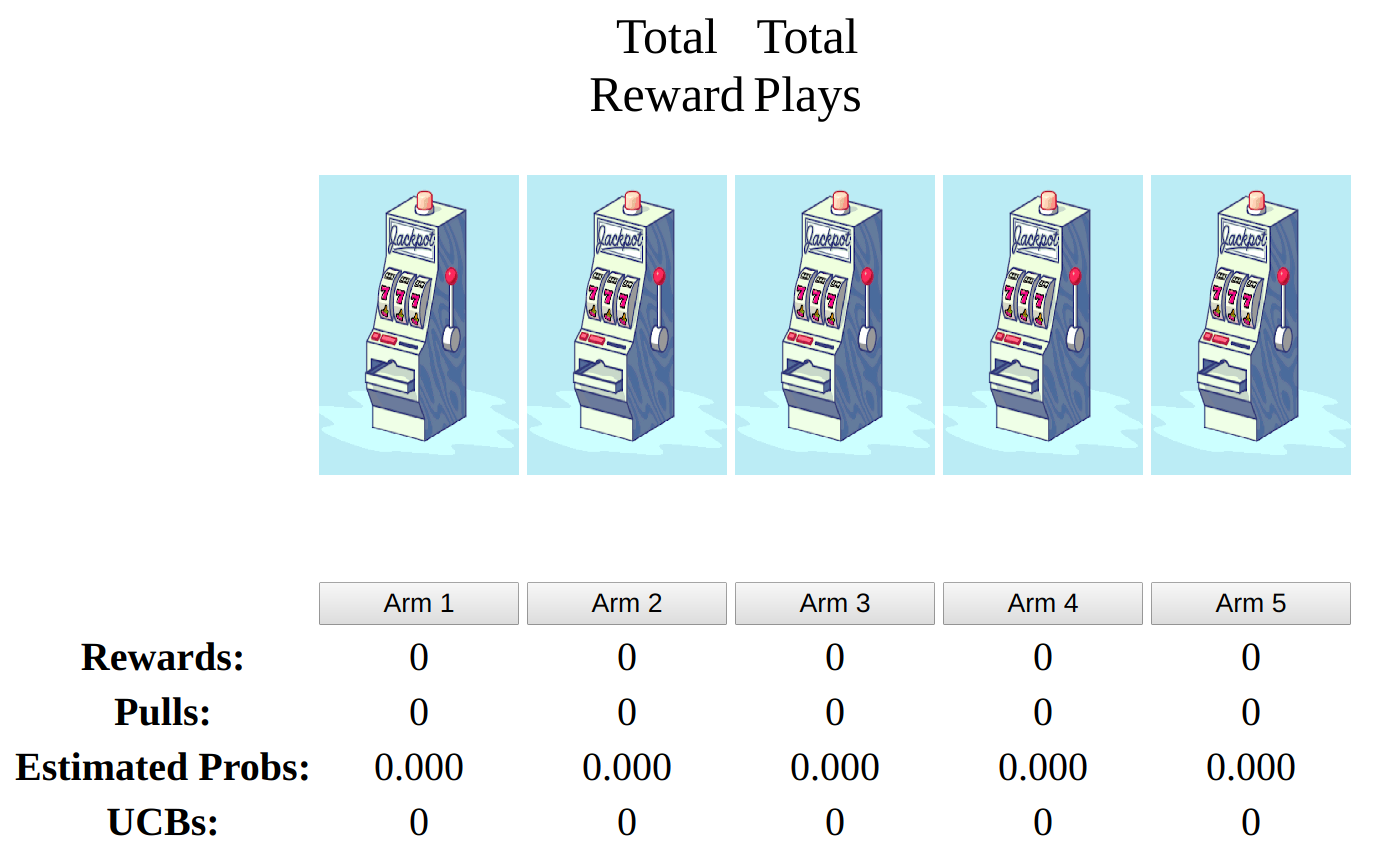
\includegraphics[width=0.75\linewidth]{2-Chapters/2-Chapter/Images/example_of_a_5_arm_bandit_problem__step0.png}
%     \caption{See }
%     \label{fig:2:example_of_a_5_arm_bandit_problem__step0}
% \end{figure}

\begin{figure}[h!]  % [htbp]
    \centering
    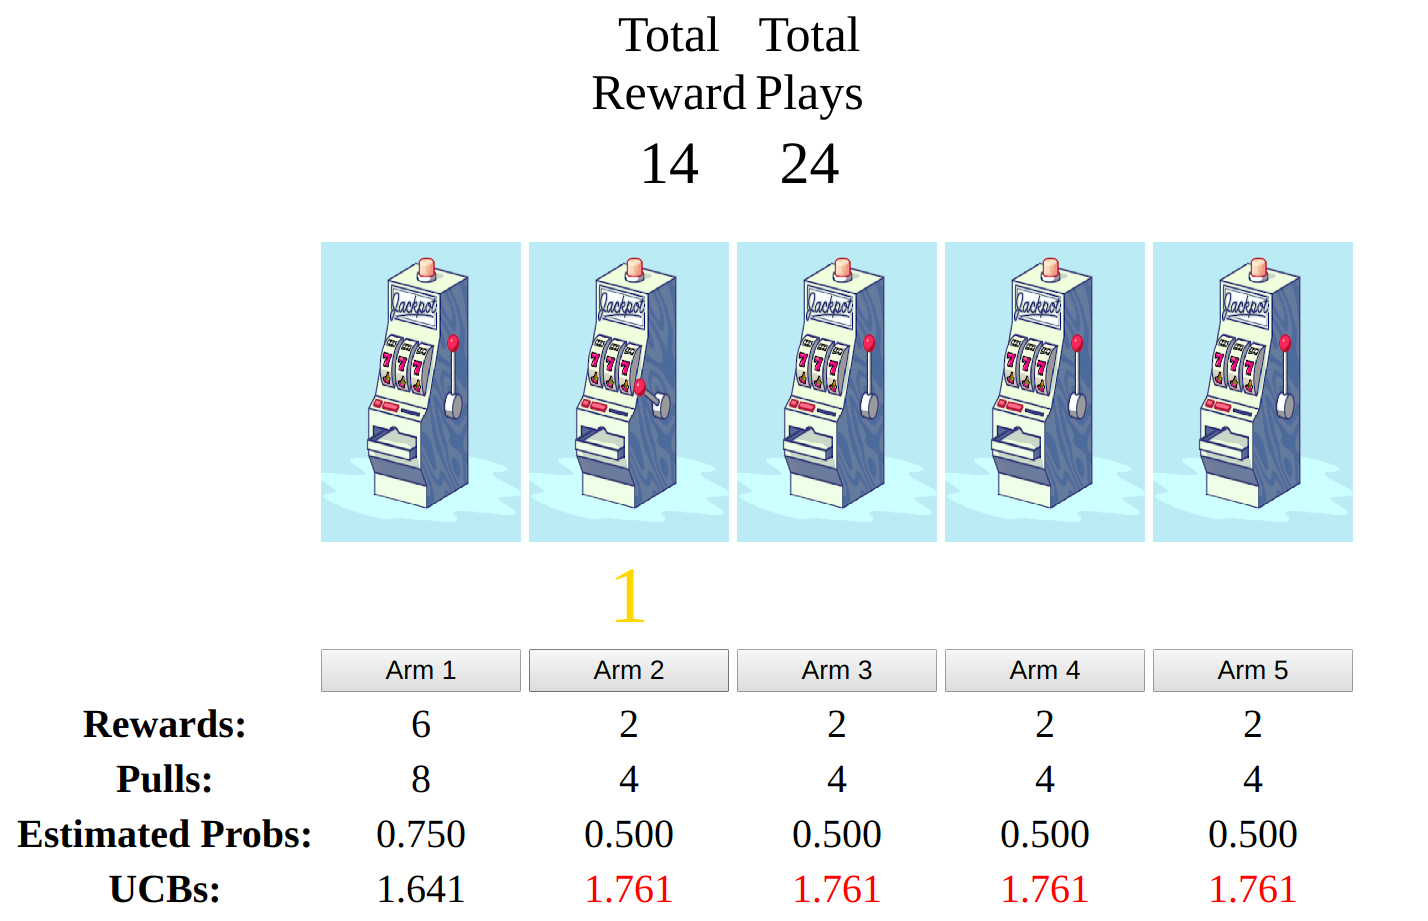
\includegraphics[width=0.85\linewidth]{2-Chapters/2-Chapter/Images/example_of_a_5_arm_bandit_problem.png}
    \caption[Screenshot of the demonstration for a current step of $t=24$.]{Screenshot of the demonstration available online on my website, for a current step of $t=24$.}
    \label{fig:2:example_of_a_5_arm_bandit_problem}
\end{figure}


The webpage looks like Figure~\ref{fig:2:example_of_a_5_arm_bandit_problem} below.
The arms follow Bernoulli distributions, \ie, $\nu_k = \mathcal{B}(\mu_k)$, of unknown means $\mu_k\in[0,1]$, and your goal in this interactive demonstration is to obtain the highest possible cumulated reward in $T=100$ steps, \ie, to maximize $\sum_{t=1}^{100} r(t)$.
Your decisions are made sequentially: at time $t$, you pick one of the arms, $A(t) \in\{1,2,3,4,5\}$, then the demo shows the random reward obtained from this (virtual) casino machine (in \textcolor{gold}{yellow}), \ie, the binary value $r(t)\in\{0,1\}$, that is sampled \iid{} from $\nu_k$.
%
The UI of the demo also shows the current value of $t$ (``total plays'') and $\sum_{s=1}^t r(s)$ the ``total reward''.
For each arm, we show the sum of rewards obtained from that arm, \ie, $X_k(t) \eqdef \sum_{s=1}^t r(s) \mathbbm{1}(A(s) = k)$, in the ``Rewards'' line, and the number of pulls of that arm, \ie, $N_k(t) \eqdef \sum_{s=1}^t \mathbbm{1}(A(s) = k)$ in the ``Pulls'' line.
%
The demo also shows the estimated probability of each arm, that is $\widehat{\mu_k}(t) \eqdef X_k(t) / N_k(t)$ (when $N_k(t)>0$), in the ``Estimated Probs'' line.

In the first Figure~\ref{fig:2:example_of_a_5_arm_bandit_problem}, the current state of the game is shown at time $t=24$.
% Currently at time $t=24$ (out of $T=100$ total time steps),
At this step, the player has collected a sum of rewards of $14$, by observing $X(t) = [6,2,2,2,2]$ rewards of value $1$ in the $K=5$ different arms. Arms were sampled $N(t) = [8,4,4,4,4]$ times, meaning that the value $0$ was seen respectively $[2,2,2,2,2]$ times, and currently arm $1$ appears to be the best one. The true means of the arms are $\bm{\mu}=[0.6, 0.2, 0.55, 0.7, 0.5]$, and (much) more samples are needed before the player can accurately identify arm $4$ as the best arm.
%
In the second Figure~\ref{fig:2:example_of_a_5_arm_bandit_problem__step100} below, we display the result of an example of run, when the player was following the $\UCB_1$ algorithm from \cite{Auer02} (we present it below in Section~\ref{sub:2:IndexPolicies}).
After $T=100$ steps, the player obtained a cumulated reward of $56$, by playing mostly arms $4,3,5,1,0$ (in decreasing order of number of plays). The empirical means $\widehat{\mu_k}(T)$ correctly identify the best arm (arm $4$), but do not correctly rank the arms as arms $1$ and $3$ obtained means of $\widehat{\mu_1}(T) = 0.5 < \widehat{\mu_3}(T)=0.6$ but the true means are $\mu_3 = 0.55 < \mu_1 = 0.6$.
Other examples of such results, for different algorithms, and $T=100$ or $T=10000$, are given in Section~\ref{sub:2:shortNumericalExperiments}.

\begin{figure}[h!]  % [htbp]
    \centering
    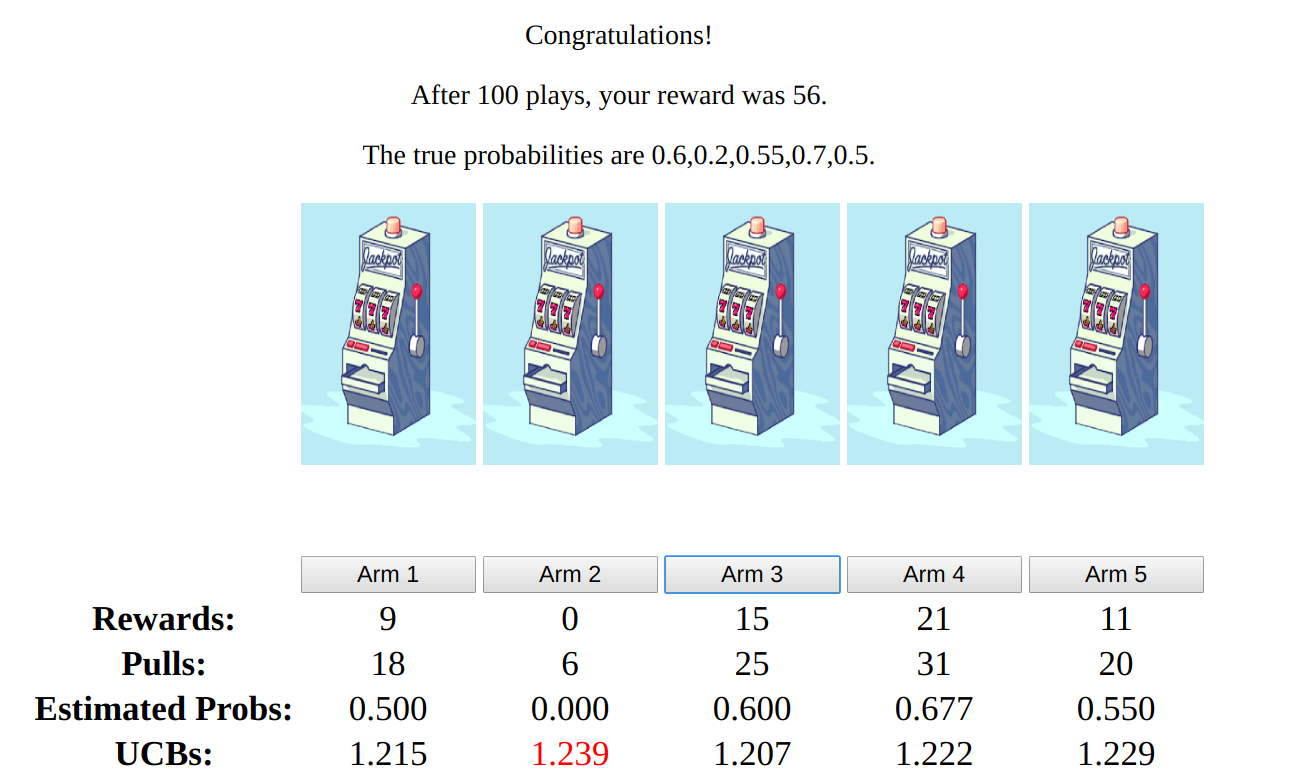
\includegraphics[width=0.85\linewidth]{2-Chapters/2-Chapter/Images/example_of_a_5_arm_bandit_problem__step100.png}
    \caption[Screenshot of the demonstration, at the end of the game after $T=100$ steps]{Screenshot of the demonstration, at the end of the game after $T=100$ steps, where the player suffers from an empirical regret of $R^{\UCB_1}_T = \mu^* T - 56 = 0.7 T - 56 = 14$ after following the $\UCB_1$ algorithm.
        You can try it on \href{https://perso.crans.org/besson/phd/MAB\_interactive\_demo/}{\texttt{perso.crans.org/besson/phd/MAB\_interactive\_demo/}}}
    \label{fig:2:example_of_a_5_arm_bandit_problem__step100}
\end{figure}


\paragraph{Decisions can (and should) depend on the past observations.}

A \emph{bandit algorithm} $\cA$ is also referred to as a strategy or a policy.
% and sometimes it is denoted by $\pi$ or $\rho$ in the literature.
The algorithm $\cA$ selects an arm $A(t)$ at time $t$, possibly by using the past observations and the past external randomness.
As shown below, being oblivious to the past yields very poor performance (cf. the pure exploration policy in Section~\ref{sub:2:naiveSimpleStrategies}), so efficient policies indeed depend on the successive feedbacks.
%
More formally, an algorithm can be defined as a sequence of \emph{measurable} functions $(\cA_t)_{t\geq1}$,
where $\cA_t$ maps the past observations $O_t \eqdef (U_0, Y_{A(1),1}, U_1, \dots, Y_{A(t-1),t-1}, U_{t-1})$
to an arm $\cA_t(O_t) \eqdef A(t) \in[K]$
(we remind that we denote $r(s) = Y_{A(s),s}$ the $s$-th reward).
The initial information is reduced to $O_1 = (U_0)$, and the first decision is $A(1) = \cA_1(O_1)$. Usually, most algorithms starts by selecting $A(1)=1,\dots,A(K)=K$ (or a permutation of the $K$ arms) in the $K$ first steps $t=1,\dots,K$ (\eg, Algorithm~\ref{algo:2:indexPolicy}).
% as illustrated for example in Algorithm~\ref{algo:2:indexPolicy} below.
%
An algorithm is said to be \emph{deterministic} if it does not depend on the external randomness $U_0,U_1,\dots$, but in this thesis \textbf{we only use non-deterministic algorithms}
(in particular, index policies need $U_t$ to break ties in the $\argmax$, see Algorithm~\ref{algo:2:indexPolicy} below).


% ----------------------------------------------------------------------------
\subsection{Common assumptions on the reward distributions}

In the example above, we consider Bernoulli distributions, but other real-valued distributions have been studied in the literature.
From now on and until the last chapter of this thesis, \textbf{we only consider stochastic rewards}. The piece-wise stationary model is studied in Chapter~\ref{chapter:6}.
%
% Everything is implemented and documented at
% https://smpybandits.github.io/docs/Arms.html
\textbf{We also focus only on real-valued rewards}, meaning that $Y_{k,t}\in\R$ for all arm $k$ and time $t$.

An important hypothesis is whether rewards are bounded or not,
and whether the player knows if they are bounded or not before starting the bandit game.
Moreover, if rewards are known to be bounded, let say in an interval $[a,b]$, another important hypothesis is whether the player knows the values of $a$ and $b$ or not.
%
Intuitively, the bandit game is easier if the player knows the support of the distributions, and we restrict to this case in all the thesis, \ie, \emph{$a,b$ are always supposed to be known}.
Most of the algorithms proposed in the literature follow this hypothesis as well.
%
The mostly used
infinitely supported distributions are Gaussian, exponential and Poisson,
while in the literature, the Bernoulli distribution is the most common case of finitely supported distributions.
Continuous-valued distributions with finite support also included truncated versions of infinitely supported distributions, in particular \emph{truncated} Gaussian are used for numerical experiments in lots of research articles.

% Just bounded, in $[a,b]$ but without loss of generality in $[0,1]$ etc.
\paragraph{The normalization trick.}
\label{par:2:normalizationTrick}
%
If the player knows that reward are bounded in an interval $[a,b]$, and if she knows $a$ and $b$ (for $a<b$), then with no loss of generality we can restrict to the interval $[0,1]$, as if $r\in[a,b]$, the player can instead consider the normalized reward $r' = \frac{r-a}{b-a}$ that lies in $[0,1]$.
Note that this ``normalization trick'' is implemented for any policy in our library SMPyBandits, with the \texttt{lower} and \texttt{amplitude} optional arguments, respectively representing $a$ the lower-bound on rewards and $b-a$ the length of the interval of possible values of rewards.

% Bernoulli, Gaussian, sub-Bernoulli, sub-Gaussian, Exponential, sub-Exponential...

\paragraph{One-dimensional exponential family.}
%
% On one-dimensional exponential family...

In the literature, parametric assumptions on the rewards are sometimes considered, typically the assumption that rewards belong to a real-valued distribution lying in an exponential families.
%  or bounded distributions.
One-dimensional exponential families include Bernoulli and Poisson distributions, as well as Gaussian distributions with a fixed variance.
Our main interest is Bernoulli distributions, but we prefer to present the more general notations of exponential families in one dimension.
% We follow the notations from the course on statistical learning (Stat 260) taught in 2010 by Michael Jordan at the University of Berkeley \cite{JordanCourseStatBerkeley}, that are also the notations used for instance in Emilie Kaufmann's PhD in 2014 \cite{Kaufmann12PhD}.

Given a measure $\lambda$, that is usually the natural Lebesgue measure on $\R$, an exponential family of probability distributions is defined as the distributions whose density (relative to $\lambda$) can be written as
% \begin{equation}\label{eq:2:exponentialFamily}
$ \Pr_{\eta}(x | \lambda) = h(x) \exp \left( \eta x - A(\eta) \right)$,
% \end{equation}
for a parameter vector $\eta$ (the canonical parameter),
% and a sufficient statistic that we restrict to be $T(x)=x$,
and a function $h$.
The cumulant function $A(\eta)$ is entirely determined by $\eta$ and $h$,
as $A(\eta) = \log \left( \int h(x) \exp(\eta x) \lambda(\mathrm{d} x) \right)$.
%
The natural parameter space is the set of values of $\eta$ such that this integral $A(\eta)$ is finite,
and usually the literature focusses on regular and minimal exponential families (when the natural parameter space is an non-empty open set in $\R$).

We mention two important results on exponential families:

\begin{enumerate}
    \item
    \emph{A distribution in such family is entirely characterized by its parameter $\eta$}.
    And the mapping $\eta \mapsto \E_{\eta}[X]$ is one-to-one,
    if $\E_{\eta}$ is the expectation under the probabilistic model $\bP_{\eta}$.
    That is why one-dimensional distributions are entirely characterized by their mean, $\mu = \E_{\eta}[X]$.

    \item
    A second important result is a simplified form for the \emph{Kullback-Leibler divergence} \cite{KullbackLeibler51}, for two distributions lying in the same exponential family.
    The KL divergence is also called the \emph{relative entropy},
    and it is a measure of how one probability distribution is different from a second, reference probability distribution.
\end{enumerate}

\begin{definition}\label{def:2:KLDivergence}
\begin{leftbar}[defnbar]  % XXX leftbar defnbar, comment if needed
    The \emph{Kullback-Leibler divergence} between distributions
    with densities $d_1$ and $d_2$, wrt to $\lambda$, is defined as
    \begin{align}\label{eq:2:Kullback-LeiblerDivergenceExpFamily1}
        \KL\left(d_1, d_2\right) \eqdef \int d_1 \log\left(\frac{d_2}{d_1}\right) \lambda(\mathrm{d}x) = \E_{d_1} \left[ \log\left(\frac{d_2}{d_1}\right) \right] \in \mathbb{R}\cup\{\pm\infty\}.
    \end{align}
% \vspace*{-5cm}  % FIXME vspace negative to compensate the \end{leftbar}
\end{leftbar}  % XXX leftbar defnbar, comment if needed
\end{definition}

Following this Definition~\ref{def:2:KLDivergence} for two distributions
$d_1=\Pr(x|\eta_1)$ and $d_2=\Pr(x|\eta_2)$,
we can use a shorter notation and write $\KL( \eta_1, \eta_2 ) \eqdef \KL(\Pr(x|\eta_1), \Pr(x|\eta_2))$, which can be simplified to use only the two parameters $\eta_1$ and $\eta_2$ of $d_1$ and $d_2$,
and $\mu_1 = \E_{\eta_1}[X]$ the mean of distribution $d_1$,
%
% \begin{equation}\label{eq:2:Kullback-LeiblerDivergenceExpFamily2}
$\KL\left( \eta_1, \eta_2 \right) = \E_{d_1}[ (\eta_1 - \eta_2) X ] - A(\eta_1) + A(\eta_2) = (\eta_1 - \eta_2) \mu_1 - A(\eta_1) + A(\eta_2)$.
% \end{equation}
%
Without diving more in the details of exponential families,
it is interesting to illustrate this definition and the notations with two important examples:

\label{par:2:notationsExponentialFamiliesBernoulliGaussian}
\begin{itemize}
    \item
    % $\bullet$
    \textbf{Bernoulli distributions} can be seen as an exponential family with $h(x) = 1$,
    and for a Bernoulli distribution of mean $\mu\in[0,1]$, denoted $B(\mu)$,
    the parameter is $\eta = \mu / (1 - \mu)$, giving $A(\eta) = \log(1 + \mathrm{e}^{\eta})$
    (with the limit behavior $\eta=+\infty$ if $\mu=0$).

    The KL divergence between $B(x)$ and $B(y)$, of parameters $\eta$, $\eta'$ is given by
    $\kl(x,y) \eqdef \KL_{B}(\eta,\eta') = x \log(x/y) + (1-x) \log((1-x)/(1-y))$,
    and it is also called the \emph{relative binary entropy}.
    It satisfies $\kl(x,y) \geq d_{1/4}(x,y)$ (Pinsker's inequality).

    \item
    % $\bullet$
    \textbf{Gaussian distributions of a known variance} are a one-dimensional exponential family,
    and in this thesis we do not consider Gaussian with an unknown variance.
    For a variance of $\sigma^2$, the family uses
    % $T(x) = [x ; x^2]^T$ and
    $h(x) = 1/\sqrt{2\pi\sigma^2} \exp(-x^2/(2\sigma^2))$,
    and for a Gaussian distribution with mean $\mu\in\R$, denoted $\cN(\mu,\sigma^2)$,
    the parameter is $\eta = \mu/\sigma^2$, giving $A(\eta) = \mu^2/(2\sigma^2)$.
    % % For a generic variance,
    % This shows that the Gaussian distributions
    % % are a two-dimensional exponential families,
    % with a fixed variance $\sigma^2$ form indeed a one-dimensional exponential family.

    The KL divergence between $\cN(x,\sigma^2)$ and $\cN(x,\sigma^2)$, of parameters $\eta$, $\eta'$ is given by
    $d_{\sigma^2}(x,y) \eqdef \KL_{\cN,\sigma^2}(\eta,\eta') = (x-y)^2 / (2\sigma^2)$
    (see Chapter~8 of \cite{JordanCourseStatBerkeley}).
\end{itemize}


\paragraph{Hypotheses in this thesis.}
%
In the rest of this thesis, \textbf{we only consider bounded rewards in the mathematical developments}, and we mostly focus on Bernoulli distributions, because they are usually the most relevant choice for the considered applications.
% First, we restrict for simplicity to Bernoulli distributions for the simulations shown in Chapter~\ref{chapter:3}, even if our library does implement all the distributions commonly found in the literature (including unbounded one-dimensional exponential families and even Markov models).
In Chapter~\ref{chapter:4}, we only study models with binary rewards.
%
Then, when we study multi-players bandits in Chapter~\ref{chapter:5}, we explain that restricting to the Bernoulli case is interesting and not restrictive, as it is actually the hardest case (since continuous distributions has a null mass on $Y_{k,t}=0$, they yield a much simpler problem as the sensing/no sensing distinction no longer makes sense), but this work can be extended to any one-dimensional exponential families.
%
Finally, in Chapter~\ref{chapter:6} we analyze our proposed algorithm for bounded distributions, without restricting to Bernoulli distributions, but we use the fact that bounded distributions on $[0,1]$ are sub-Bernoulli, and we use the Bernoulli Kullback-Leibler divergence $\kl$ in our analysis.


\paragraph{Sub-Gaussian and sub-Bernoulli distributions.}
%
A lot of research works considers rewards distributions that are not Gaussian but sub-Gaussian,
% of a known variance, for instance $1/4$.
meaning distributions whose moment generating function is dominated by that of a Gaussian distribution with the same mean (and a known variance).
For instance, bounded distributions on $[0,1]$ are known to be $1/4$ sub-Gaussian, and this fact is used for instance in \cite{Maillard2018GLR}.
In Chapter~\ref{chapter:6}, we instead consider sub-Bernoulli distributions, formally introduced in Definition~\ref{def:6:subBernoulliDistributions}.
%
Such hypothesis is also proposed for other families of distributions, for instance the recent article \cite{KimTewari2019} analyses their Follow-the-Perturbed-Leader algorithm for perturbations following any sub-Weibull distribution (sub-Weibull distributions generalize both sub-Gaussian and sub-Exponential distributions).



\paragraph{About Markov models.}
%
% Markov models: we do not present it in this thesis.
Finally, we note that Markov bandit models have also been considered for Cognitive Radio applications \cite{Liu08}.
They are not studied in this thesis, even though we did implemented them in SMPyBandits,
They were introduced in the $1980$s, by Whittle in \cite{Whittle1988} and Anantharam and others in \cite{Anantharam87b}.
A Markov MAB model maps an arm to a Markov chain \cite{Norris98}, instead of a distribution, and thus they are no longer stochastic nor stationary.
Such Markov models come in two flavors: rested or restless.
For $K$ arms, each Markov chain has a finite number of states $s$, each corresponding to a (constant) reward that the player obtains if she selects this arm while its Markov chain is in state $s$.
Rested Markov models means that only the state of the selected arm's Markov chain can change, following its Markov transition matrix.
Restless models remove this hypothesis, making them harder to track and solve.
%
Such models were less studied than stationary or adversarial models, but some interesting works applied Markov models or CR applications in the last 10 years
For instance, \cite{Melian15} proposed a CR model mixing MAB and Hidden Markov Models (HMM), solved by a mixed policy called UCB-HMM.
A curious reader about Markov chains could start to read Chapter~3 of \cite{LattimoreBanditAlgorithmsBook} (Section~3.2) and refer to \cite{Norris98}.


% ----------------------------------------------------------------------------
\section{Applications of stochastic MAB}
\label{sec:2:applicationsofStochasticMAB}

The blooming success of the research on multi-armed bandits is easily explained by the different spectrum of applications of MAB models to real-world discrete-time decision making problems.
This research field has been very active since the years 2010s, but it started as early as 1933 with \cite{Thompson33}, and was active since the 1980s and the seminal works by Lai and Robbins \cite{LaiRobbins85} and by Anantharam and others \cite{Anantharam87a}.
%
MAB have been applied successfully to various decision making problems, like the following:

\textbf{Clinical trials} have been the first historical application of MAB models, where an arm represents a treatment, and the distribution associated with such treatment can be a Bernoulli distribution: a reward of $0$ means the drug did not heal the disease, and a reward of $1$ indicates a success. The mean of an arm, in this application, represents the mean success rate of a treatment.
Following the ``best arm identification'' model, the goal of a doctor in a clinical trial is to identify the best treatment, \ie, the arm with highest mean, in a number of trials as short as possible.
And following our model of interest, maximizing the rewards corresponds to maximize the number of patients being successfully treated.
%
% After introducing formally the notations used in all this thesis, we review below possible applications of multi-armed bandits.

% Other popular applications include the following.
%
% \begin{itemize}
%     \item
    % \textbf{A/B testing}, for instance for websites, is a popular application of the best arm identification problem,
    % where the task is purely exploratory and the player is asked to identify the best of two options (or more), in a finite number of steps \cite{audibert2010best}.
    % The problem can either consider a fixed budget and no freedom on the ending of the game (\ie, an known horizon $T$), or a fixed confidence and a certain freedom on the budget (\ie, the identified arm must be the true best arm with probability at least $1-\delta$) \cite{Garivier16BAI}.
    % The theoretical complexity of this problem
    % % use of bandit for A/B testing
    % was first studied in \cite{Kaufmann14},
    % and a more practical point-of-view was proposed in \cite{Jamieson17ABTest}.

    % \item
    MAB can also be applied to a broader setting of \textbf{online content recommandation},
    with more than two options.
    The seminal work of \cite{Li10} studies the application of contextual bandit to news article recommendation, as it is used in practice on platforms such as Microsoft's Bing news website,
    or in applications like Netflix.
    In such models, the arms correspond to items to recommend (\eg, articles or movies), and the contexts contain features about each user of the system.
    An interesting work is \cite{Louedec16}, who studies slowly-varying non-stationary models applied to recommender systems.

    % \item
    Using bandit algorithms for \textbf{improved machine learning} models or algorithms has been an active research domain for the last ten years or so.
    As presented below in Chapter~\ref{chapter:25}, a certain ``leader'' bandit algorithm can be used to select on the run the best bandit algorithm from a pool of ``followers'' algorithms.
    Other possible use cases include hyper-parameter optimization, or features selection.
    Hyper-parameters include real-valued parameters,
    % like $\alpha\in[\frac{1}{2},\infty)$ for the $\UCB_1$ or $\varepsilon\in(0,1)$ for the $\varepsilon$-greedy bandit algorithms,
    like a step size multiplier $\gamma$ in a gradient descent,
    the width $\rho$ of a Radial Based Function (RBF) kernel,
    the margin $C$ in a Support Vector Machines (SVM), etc.
    Discrete-valued parameters are also common, like a choice in a fixed set of kernel functions or the depth of neural networks,
    and higher dimensional or more complex hyper-parameters can for instance be the entire architecture of a neural network.


\textbf{Applications for Cognitive Radio.}
% Detail the previous work from our team SCEE on bandits + OSA : Wassim, Navik
%
As highlighted in Chapter~\ref{chapter:1},
the focus of this work is on cognitive radio and IoT networks, where arms can represent wireless orthogonal channels, but more generally any resource characterizing the communication between a wireless device and a gateway (\eg, spreading factor for LoRa \cite{KerkoucheAlami18}, power allocation for NOMA etc).
% In cognitive radio using centralized supervision, for instance if the gateway can decide the allocation of devices to resources, MAB can also be used to let the gateway explore different allocations and learn by itself a good allocation, see for instance this article that consider 5G-like networks with small cells \cite{Maghsudi16}.
%
% Previous works of our SCEE team showed that MAB can be used to model the problem of spectrum access for a secondary user accessing a licensed spectrum.
% In this model, arms represent a finite set of orthogonal channels, \ie, different frequency bands in a licensed spectrum.
In the model of Opportunistic Spectrum Access (OSA) with sensing \cite{Jouini09,Jouini10}, the samples $Y_{k,t}$ represents the feedback obtained by the CR-equipped device after sensing the channel $k$ at time $t$.
A reward of $r(t) = 1$ indicates that no Primary User was sensed, while a reward of $r(t)=0$ indicates that the channel $k$ is busy at time $t$ and no uplink message can be sent.
% %
% This model was first introduced by W. Jouini during his PhD thesis,
% in \cite{Jouini09} and later studied in both \cite{Jouini10,Jouini12}.
% Proof-of-concepts using real-world radio hardware were first proposed in \cite{MoyWSR2014,RobertSDR2014}.
%
We study a similar model of using MAB for Cognitive Radio but without the OSA structre of Primary and Secondary users, \ie, without sensing information but only a collision indicator, in Chapters~\ref{chapter:4} and \ref{chapter:5}.


The different applications discussed in this Section are still active research directions,
and a curious reader can find other interesting applications of MAB models and algorithms in \cite{bouneffouf2019survey}, such as game tree search or network routing in Section~1.2 of \cite{LattimoreBanditAlgorithmsBook}.


% ----------------------------------------------------------------------------
% \section{Definition, decomposition and lower-bounds on the regret}
\section{Measuring the performance of a MAB algorithm}
% : definition, decomposition, and lower bounds
\label{sec:2:lowerUpperBoundsRegret}

As explained above, the main objective of a player facing a bandit game is to maximize its (expected) cumulated reward.
%
In particular, an efficient algorithm should see its mean reward converge to the maximum reward.
In the bandit literature, the performance of an algorithm is often measured in terms of regret, a performance measure that we now introduce.
% We introduce in this section the notion of \emph{regret}, and the equivalence for a player between maximizing its sum of rewards and minimizing its regret.
% In Machine Learning, we usually prefer to aim at minimizing certain quantities, such as the error rate in supervised learning, or the distance to the optimum in an optimization problem,
% but the main interest of studying the regret is to be able to obtain higher-order information about the convergence of the mean reward to the max reward,
% or in other words, to quantify the speed of convergence of a MAB algorithm.


\subsection{Measuring performance with the (mean) regret}

Let us first introduce some notations.
We consider a stochastic and stationary MAB problem, with $K$ arms of distributions $\nu_1,\dots,\nu_K=(\nu_k)_k$, that generates \iid{} samples $Y_{k,t} \sim \nu_k$, for any time $t$.
% with $r(t)=Y_{A(t),t}$).
We focus on distributions fully characterized by their means, that can be Bernoulli or any one-dimensional exponential family.
We denote $\mu_k \eqdef \E[Y_{k,t}] \in \R$ the mean of the distribution of arm $k$ (it will be referred to as the \emph{mean of arm $k$}).
%
% \paragraph{Defining the regret.}
%
To define the regret, we first need to distinguish between \emph{optimal} and \emph{sub-optimal} arms.

\begin{definition}\label{def:2:optimalSubOptimalArms}
\begin{leftbar}[defnbar]  % XXX leftbar defnbar, comment if needed
    % [Optimal and sub-optimal arms]
    Consider a bandit problem of $K$ arms with distributions of means $\bm{\mu}=\mu_1,\dots,\mu_k$.
    Denote $\mu^* \eqdef \max_k \mu_k$ the largest mean.
    The best arm can be non unique, and any arm $k$ having $\mu_k = \mu^*$ is said to be \emph{optimal},
    while arms satisfying $\mu_k < \mu^*$ are called \emph{sub-optimal}.
\end{leftbar}  % XXX leftbar defnbar, comment if needed
\end{definition}

If the goal of the player is to maximize $\E\left[\sum_{t=1}^T r(t)\right]$,
the optimal strategy for this bandit problem is to always pull one of the optimal arms (it can be not unique), but it is unrealistic as the player does not know the true means, nor the optimal arms (as long as they are not all optimal, \ie, in non trivial problems).
%
Comparing the difference between the performance of a fixed baseline and that of the player is a common approach in machine learning research,
and here we can compare with the oracle strategy that always obtains an (expected) reward of $\mu^*$.
%
For a fixed horizon $T$, if $k^*$ denotes the index of any optimal arm,
let us introduce the (mean) regret $R_T^{\cA}$ of an algorithm $\cA$ as
$R_T^{\cA} \eqdef \E\left[ \sum_{t=1}^T (Y_{k^*,t} - r(t)) \right]$.
%
As the rewards from arm $k^*$ are \iid{} (as for all arms), and by linearity of the expectation, we can rewrite this expression to obtain the following definition of the regret.
% \begin{align*}
%     R_T^{\cA}
%     & = \E\left[ \sum_{t=1}^T (Y_{k^*,t} - r(t)) \right]
%     = \E\left[ \sum_{t=1}^T \underbrace{Y_{k^*,t}}_{\text{\iid{} from $\nu_{k^*}$}} \right] - \E\left[ \sum_{t=1}^T r(t) \right] \\
%     & = T \times \E\left[ Y_{k^*,1} \right] - \sum_{t=1}^T \E\left[ r(t) \right]
%     = T \mu^* - \sum_{t=1}^T \E\left[ r(t) \right].
% \end{align*}
% % This is the definition we give below.


\begin{definition}[Regret]\label{def:2:regret}
\begin{leftbar}[defnbar]  % XXX leftbar defnbar, comment if needed
    For an algorithm $\cA$, a bandit problem of $K$ arms characterized by their means $\mu_1,\dots,\mu_K$, with $\mu^* \eqdef \max_k \mu_k$, then its \emph{(mean) regret} at horizon $T$ is $R_T^{\cA}$ defined as
    %
    \begin{align}\label{eq:2:regret}
        R_T^{\cA}
        & = \E\left[ \sum_{t=1}^T (Y_{k^*,t} - r(t)) \right]
        = \E\left[ \sum_{t=1}^T \underbrace{Y_{k^*,t}}_{\text{\iid{} from $\nu_{k^*}$}} \right] - \E\left[ \sum_{t=1}^T r(t) \right] \\
        & = T \times \E\left[ Y_{k^*,1} \right] - \sum_{t=1}^T \E\left[ r(t) \right]
        = T \mu^* - \sum_{t=1}^T \E\left[ r(t) \right].
    \end{align}
% \vspace*{-20pt}  % FIXME vspace negative to compensate the \end{leftbar}
\end{leftbar}  % XXX leftbar defnbar, comment if needed
\end{definition}

One first need to observe that $R_T^{\cA} \geq 0$ for any $T$ and $\cA$, and that $R_T^{\cA} \leq \mu^* T$, so $R_T^{\cA} \leq T$ if the rewards lie in $[0,1]$.
Thus any algorithm has $R_T^{\cA} = \bigO{T}$, which justifies why we are interested in efficient algorithms that achieve at least a sub-linear regret, \ie, $R_T^{\cA} = \smallO{T}$.

\paragraph{A useful decomposition of the regret.}
%
Recall that $N_k(t) \eqdef \sum_{s=1}^t \mathbbm{1}(A(s) = k)$ denotes the number of times arm $k$ was selected between times $1$ and $t$,
%
and that the samples $Y_{k,t}$ are all \iid{} of mean $\mu_k$.
The \emph{gap} between any arm $k\in[K]$ and an optimal arm is defined as $\Delta_k \eqdef \mu^* - \mu_k$
(an arm $k$ is thus sub-optimal if and only if $\Delta_k > 0$),
and thus we can write the following decomposition on the regret.
%
\emph{Its proof is simple and it is not a contribution, but we include it for readers that are unfamiliar with conditioning arguments}.

\begin{proposition}[Regret decomposition]\label{prop:2:RegretDecomposition}
\begin{leftbar}[propositionbar]  % XXX leftbar propositionbar, comment if needed
    The (mean) regret $R_T^{\cA}$ can be decomposed as a sum of the number of selections of sub-optimal arms $k$, weighted by their gaps:
    \begin{align}\label{eq:2:RegretDecomposition}
        R_T^{\cA} = \sum_{k=1}^K \Delta_k \; \E[ N_k(T) ]
        = \sum_{\substack{k=1,\dots,K\\\Delta_k > 0}} \Delta_k \; \E[ N_k(T) ].
    \end{align}
    % \vspace*{-20pt}  % FIXME vspace negative to compensate the \end{leftbar}
\end{leftbar}  % XXX leftbar propositionbar, comment if needed
\end{proposition}
%
\begin{smallproof}\label{proof:2:RegretDecomposition}
    We use the chain rule of expectation and a conditioning on $O_t$,
    because the expectation is taken on the randomness of the (\iid) samples $(Y_{k,t})_t$ and on the decisions of the player $(A(t))_t$, which are measurable wrt to the past observations $O_t = (U_0, Y_{A(1),1}, U_1, \dots, Y_{A(t-1),t-1}, U_{t-1})$.
    Thus we can rewrite the expected cumulated reward as follows:
    %
    % FIXME add a blank line or a negative space if it looks weird
    %
    % \vspace*{-20pt}
    \begin{align*}
        \E \left[ \sum_{t=1}^T r(t) \right]
        &= \E \left[ \sum_{t=1}^T \sum_{k=1}^K Y_{k,t} \mathbbm{1}(A(t) = k) \right]
        = \sum_{k=1}^K \sum_{t=1}^T \E \left[ Y_{k,t} \mathbbm{1}(A(t) = k) \right] \\
        &= \sum_{k=1}^K \sum_{t=1}^T \E \Bigl[ \E \left[ Y_{k,t} | O_t \right] \mathbbm{1}(A(t) = k) \Bigr]
        = \sum_{k=1}^K \sum_{t=1}^T \E \Bigl[ \E \left[ Y_{k,1} \right] \mathbbm{1}(A(t) = k) \Bigr] \\
        &= \sum_{k=1}^K \underbrace{\E \left[ Y_{k,1} \right]}_{\mu_k} \underbrace{\sum_{t=1}^T \E \left[ \mathbbm{1}(A(t) = k) \right]}_{= N_k(T)}
        % = \sum_{k=1}^K \mu_k \E \left[ \sum_{t=1}^T \mathbbm{1}(A(t) = k) \right]\\
        = \sum_{k=1}^K \mu_k \E \left[ N_k(T) \right].
    \end{align*}
    %
    Thus $R_T^{\cA} = T \mu^* - \sum_{t=1}^T \E\left[ r(t) \right] = T \mu^* - \sum_{k=1}^K \mu_k \E[ N_k(T) ] = \sum_{k=1}^K (\mu^* - \mu_k) \E[ N_k(T) ]$,
    as $\sum_{k=1}^K  \E[ N_k(T) ] = T$.
    The sum is then simplified to only count sub-optimal arms.
\end{smallproof}


\paragraph{Consequences.}
%
Such decomposition of the regret can be useful for at least two reasons:

% \begin{itemize}
%     \item
On the one hand, from a numerical simulation point-of-view, when we run a finite number of repetitions of the same stochastic experiment, if we want to compute and visualize the regret, we can either use the definition with the rewards, or the decomposition and simply sum the gaps $\Delta_k$ with the number of sub-optimal draws.
Both quantities are indeed equal \emph{in expectation}, but with only a finite number of trajectories and observations, the first estimate is more noisy than the second one, since the randomness on the rewards is (partially) removed in the decomposition \eqref{eq:2:RegretDecomposition} (thanks to the conditioning on $O_t$ done in the proof).
In our library SMPyBandits, we implement both estimators, and all values of regret used in this thesis are based on the one using the decomposition of Proposition~\ref{prop:2:RegretDecomposition}, because it gives faster convergence, and also ``smoother'' plots.
\label{remark:2:moreAccurateCountofRegretForSimulations}

    % \item
On the other hand, this decomposition is necessary as theoretical analyses of the regret of (single-player) MAB algorithms are usually based on controlling the suboptimal draws $N_k(T)$ and not directly the regret $R_T^{\cA}$.
Even if we prove that controlling $N_k(T)$ is no longer sufficient to obtain low regret for the multi-players case, we extend this decomposition in Chapter~\ref{chapter:3} (in Lemma~\ref{lem:5:DecompositionRegret}), and it is the first quantity we prove to be bounded by $\bigO{\log(T)}$ when we prove the regret upper-bound of our proposal \MCTopM-\klUCB.
% \end{itemize}


\subsection{Regret lower bounds}

We include here two well-known results about what bandit algorithms \emph{cannot} do.
First, a \emph{problem-dependent lower-bound} states that any algorithm suffers a regret at least $\Omega(\log T)$ on any problem (from \cite{LaiRobbins85}).
Then, a \emph{worst-case result} states that for any algorithm, there exists a certain problem instance such that the algorithm can perform as badly as $\Omega(\sqrt{K T})$ (a result from \cite{Auer02NonStochastic}),
%
In certain families of problems, \eg, $K$ Bernoulli distributed arms, the difficulty of a problem is characterized by a constant that depends only on the arms means. This measure of difficulty of a problem is hidden in the $\Omega$ notation in these lower-bounds.

In all this section, we restrict to stationary stochastic problems with $K\geq2$ arms.
We do not give proofs of the following theorems, as they can be found in the historical papers, and simpler proofs are given in recent references, such as \cite{Bubeck12}, \cite{LattimoreBanditAlgorithmsBook}, or Chapter~2 in \cite{Slivkins2019} for instance.
%
Let $\cI$ denote the set of all problem instances, with $K \geq 2$ arms.
We assume the rewards lie in $[0,1]$,
to present the lower-bounds, we prefer to focus on Bernoulli distributions, for simplicity.
%
To specify the dependency on an instance $I\in\cI$, we denote the regret of $\cA$ on instance $I$ and horizon $T$ by $R_T^{\cA}(I)$.
We also index the Landau notations $o(\dots)$ and $\bigO{\dots}$ by $I$,
for instance $R_T^{\cA}(I) = o_I(\log(T))$ means $R_T^{\cA}(I) = \smallO{c_I \log(T)}$
where the ``constant'' $c_I$ can depend on the problem instance $I$ (\eg, on its means and on $K$) but \emph{not} on the time horizon $T$.


\paragraph{Problem-dependent lower-bound in $\Omega(\log T)$.}
%
The following two theorems were proven in \cite{LaiRobbins85}.
These lower-bounds are of highest interest to design efficient algorithms,
and a significant part of the research literature on MAB algorithms has focused on finding algorithms that matches the Lai and Robbins' lower-bound asymptotically.
This means that an upper-bound is proven on the regret of algorithm $\cA$, that asymptotically matches the lower-bound, with the same constant in the big-$\cO$ notation (in which case we say that the algorithm is asymptotically \emph{optimal}), or with a larger constant (the algorithm is said to be \emph{order-optimal} in such case).


\begin{theorem}\label{thm:2:firstLogTLowerBound}
\begin{leftbar}[theorembar]  % XXX leftbar theorembar, comment if needed
    \emph{No algorithm $\cA$ can achieve} a (mean) regret $R_T^{\cA}(I) = o_I(\log(T))$ for all Bernoulli problem instances $I \in \cI$.
    \hfill{} \cite[Theorem~2.12]{Slivkins2019}
\end{leftbar}  % XXX leftbar theorembar, comment if needed
\end{theorem}

We consider uniformly efficient\footnote{This notion is then extended to ``\emph{strongly uniformly efficient} algorithms'', in the multi-players case with Definition~\ref{def:5:DecentralizedUniformEfficiency}, where we also include a notion of (expected) fairness.} algorithms, to rule out algorithms achieving low regret on some problem instances while achieving linear regret on other instances.
In particular, it is necessary to rule out algorithms that always pick the same arm, as on some problem instances such fixed-arm algorithms can achieve zero regret.

\begin{definition}\label{def:2:uniformlyEfficientAlgorithm}
\begin{leftbar}[defnbar]  % XXX leftbar defnbar, comment if needed
    An algorithm $\cA$ is \emph{uniformly efficient} if its (mean) regret satisfies
    $R_T^{\cA}(I) = o_I(T^{\alpha})$,
    for any value $\alpha>0$ and any problem instance $I\in \cI$.
    % where this notation means that the ``constant'' $C_{I,\alpha}$ can depend on the problem instance $I$ and on $\alpha$, but \emph{not} on the time horizon $T$.
\end{leftbar}  % XXX leftbar defnbar, comment if needed
\end{definition}

This family is non-empty as it contains for instance the $\UCB_1$ algorithm, since its regret is proven to be logarithmic on any Bernoulli problem instance (in Theorem~\ref{thm:2:UCBregretBound} below).
Now we can state the second logarithmic lower-bound, for algorithms in this family.

\begin{theorem}\label{thm:2:secondLogTLowerBound}
\begin{leftbar}[theorembar]  % XXX leftbar theorembar, comment if needed
    If $\cA$ is uniformly efficient,
    then for any arbitrary Bernoulli problem instance $I$,
    its regret is asymptotically lower-bounded by $C_I \log(T)$,
    or in other words,
    \hfill{} \cite[Theorem~2.13]{Slivkins2019},
    \[ \liminf_{T\to\infty} \frac{R_T^{\cA}(I)}{\log(T)} \geq C_I. \]
    % there exists a constant $C_I$ depending only on $I$,
    % and a time $T_0$ such that $\forall T \geq T_0, \;\;\; R_T^{\cA}(I) \geq C_I \log(T)$.
\end{leftbar}  % XXX leftbar theorembar, comment if needed
\end{theorem}

We state below Theorem~2.12 from \cite{Slivkins2019}, to specify a possible value for the constant $C_I$.

\begin{theorem}\label{thm:2:forSecondLogTLowerBound}
\begin{leftbarnospace}[theorembar]  % XXX leftbar theorembar, comment if needed
    If $\cA$ is uniformly efficient,
    and $I$ an arbitrary Bernoulli problem instance.
    \begin{itemize}
        \item
        The bound from Theorem~\ref{thm:2:secondLogTLowerBound} holds with
        % \begin{equation}\label{eq:2:forSecondLogTLowerBound}
            % $C_I = \mu^* (1 - \mu^*) \sum\limits_{k: \Delta_k > 0} \frac{1}{\Delta_k}$.
            $C_I = \sum\limits_{k: \Delta_k > 0} \frac{\Delta_k}{\kl(\mu_k, \mu^*)}$.
        % \end{equation}
        \item
        For any $\varepsilon>0$, the bound also holds at finite time with
        % \begin{equation}\label{eq:2:forSecondLogTLowerBound2}
            $C'_I = C_I - \varepsilon$,
        % \end{equation}
        meaning that there exists a constant $C'_I$ depending only on $I$,
        and a time $T_0$ such that $\forall T \geq T_0, \;\;\; R_T^{\cA}(I) \geq C'_I \log(T)$.
    \end{itemize}
\end{leftbarnospace}  % XXX leftbar theorembar, comment if needed
\end{theorem}

Moreover, it is interesting to note that the second lower-bound of Theorem~\ref{thm:2:forSecondLogTLowerBound} can be directly used to design efficient algorithms\footnote{~Tracking this quantity, by using empirical estimates of the means, is used for instance in the OSSB algorithm proposed in \cite{Combes17}, which is proven to attain the lower-bound for a wider range of problems (for problems called structured stochastic bandits).}, as thanks to the regret decomposition given in Proposition~\ref{prop:2:RegretDecomposition} above, the expression of $C_I$ essentially says that any efficient algorithm
should sample each sub-optimal arm $k$ about $\log(T)/\kl(\mu_k,\mu^*)$ times in the total of $T$ time steps.


Many algorithms have been proven to achieve logarithmic regret in the stochastic case,
and in particular it is the case of the algorithms used in this thesis, $\UCB_1$ from \cite{Auer02}, Thompson sampling from \cite{Thompson33} and analyzed in \cite{AgrawalGoyal11,Kaufmann12Thompson}, and \klUCB{} from \cite{Garivier11KL,KLUCBJournal}.
%
Such bounds are valid in different settings, and in particular $\UCB_1$ is order-optimal for bounded rewards or one-dimensional exponential families,
while Thompson sampling is optimal for bounded rewards, and \klUCB{} have been proven to be optimal for both cases.
%
For more details, we refer to Chapter~16 of \cite{LattimoreBanditAlgorithmsBook}.


\paragraph{Worst-case lower-bound in $\Omega(\sqrt{T})$.}
%
For a fixed horizon $T$, it is interesting to note that one can find instances $I$ that are so ``hard'' that a logarithmic regret (lower or upper) bound that uses a constant $C_I$ no longer brings any information.
Indeed, we can naively bound the regret by $R_T^{\cA} \leq (\max_k \Delta_k) T$, and thus if $(\max_k \Delta_k)$ can be taken so small that $C_I \log(T) \gg (\max_k \Delta_k) T$, a regret upper bound like $R_T^{\cA} \leq C_I \log(T)$ is useless.
%
% \begin{smallproof}\label{proof:2:worstCaseLowerBound}
%     For an example, consider any large horizon $T>10$, and $K=2$ Bernoulli arms.
%     Chose any small $\varepsilon$ such that $\varepsilon \ll \sqrt{4 \log(T) / T}$, then chose let $\mu_1 = 1/2$ and $\mu_2 = 1/2 - \varepsilon$.
%     The constant $C_I$ from the first case of Theorem~\ref{thm:2:forSecondLogTLowerBound} is $C_I = 1 / (4 \varepsilon)$ and $\Delta=\varepsilon$ and it becomes so large that
%     the logarithmic upper-bound is useless in such case, as
%     $\varepsilon \ll \sqrt{\frac{4 \log(T)}{T}} \Longleftrightarrow \frac{1}{4\varepsilon} \log(T) \gg \Delta T$.
% \end{smallproof}

For this reason, another family of regret bounds is relevant, that are not problem-dependent but worst-case, or also called minimax \cite{Audibert2009minimax,audibert2010minimax} or problem-independent.
We give an example of such result below.
% Hence it is interesting to quote another lower-bound on the regret, that can bring useful information in such settings.
The following theorem is from \cite{Auer02NonStochastic}, and \cite[Theorem~2.1]{Slivkins2019}.
%
For more details, we refer to Chapter~15 of \cite{LattimoreBanditAlgorithmsBook}.

\begin{theorem}\label{thm:2:worstCaseLowerBound}
\begin{leftbar}[theorembar]  % XXX leftbar theorembar, comment if needed
    Fix the number of arms $K$, and an algorithm $\cA$.
    Then for any horizon $T$, there exists a Bernoulli problem instance $I_T$ on which the algorithm suffers at least a regret $R_T^{\cA}(I_T) \geq \Omega(\sqrt{K T})$.
\end{leftbar}  % XXX leftbar theorembar, comment if needed
\end{theorem}

Similarly to what is considered for the first lower-bound,
a natural question is to know if there is an algorithm achieving a regret upper-bound of the form $R_T^{\cA}(I) \leq \bigO{\sqrt{K T}}$ for any instance, independently on the problem difficulty.
The question has been answered since the early $2000$s, as it is for instance the case for the Exp3 algorithm from \cite{Auer02}.
In the last decade, some algorithms were shown to achieve both a problem-dependent logarithmic and a minimax upper-bounds,
like MOSS from \cite{Audibert2009minimax} or recently \KLUCBpp{} from \cite{Menard17},
and such results are usually referred to as ``best of both worlds''.


% % do not detail too much, don't explain the tools behind the result

% \begin{itemize}
%     \item
%     - [Lai and Robbins] lower-bound in $\Omega(\log(T))$ \cite{LaiRobbins85}
%     \item
%     - Worst case lower-bound in $\Omega(\sqrt{T})$ \cite{Auer02,Auer02NonStochastic,Bubeck12}
%     \item
%     - Adversarial lower-bound in $\Omega(\sqrt{T})$ (also useful for piece-wise stationary models) \cite{Auer02NonStochastic}
% \end{itemize}


\subsection{Other measures of performances}
\label{sub:2:otherMeasuresPerformance}

The theoretical results obtained in the rest of this thesis are all expressed in terms of the mean regret $R_T^{\cA}$ (in Chapters~\ref{chapter:5} and \ref{chapter:6}), but we quickly mention other measures of performances that we consider in our works and in this manuscript.

% - Quantile regret or just histogram of regrets
First, when doing numerical experiments about bandits, if one studies the regret as an empirical mean based on a ``large'' number of random repetitions (\eg, $N=1000$ repetitions), it is important to not only show the mean value but also the variance of the values taken by the regret on each repetition, to verify that all algorithms perform consistently.
Indeed, by only visualizing the mean of $1000$ values, it is possible that we miss some ``bad runs'': if $1$ run out of the $1000$ gives linear regret (\ie, $R_T^{\cA} \propto T$) and the $999$ other give logarithmic regret, then the mean will appear logarithmic.
This is the case of the \Selfish{} algorithm that is defined and explored in Chapter~\ref{chapter:5}.
By visualizing the entire \emph{distribution} (as an histogram), or the variance of the values of $R_T^{\cA}$, and if the number $N$ is reasonably large, we can verify that the regret appears logarithmic for all runs.

% DONE on s'en fout !
% % - Best Arm Identification?
% Other measures of performance that has been studied in the literature include
% the best arm identification (BAI) rate
% and the best arm selection (BAS) rate.
% The BAI rate counts the frequency at which an algorithm $\cA$ correctly identified the best arm(s) at the horizon $T$,
% while the BAS rate counts the total number of time steps during which $\cA$ selected (one of) the best arm(s).
% Both quantities are computed and stored in all numerical simulations using SMPyBandits, but visualizations for both have not been included in this thesis.

% - Worst case regret (max $R_T^{r}$ for $r$ index of Monte-Carlo simulation?)
The \textbf{switching cost} $\mathrm{SC}^{\cA}(T)$ counts how many times the player's decision has changed from one round to the next one, \ie, $\mathrm{SC}^{\cA}(T) \eqdef \sum_{t=1}^{T-1} \indic(A(t) \neq A(t+1))$.
It has recently gained interest in the literature, for instance the authors of \cite{Koren17} proposed an algorithm that adaptively tries to balance the trade-off between minimizing the regret and minimizing the switching cost.
%
Indeed, in single-player models it is easy to show that achieving logarithmic regret directly implies a logarithmic upper-bound on the switching cost, and conversely the lower-bound from \cite{LaiRobbins85} also gives an asymptotic logarithmic lower-bound.
But even if $\mathrm{SC}^{\cA}(T) = \Theta(\log T)$ for an efficient algorithm, it can be interesting to numerically evaluate this quantity, as a large value might indicate an algorithm that is alternating too much between the optimal arm and other arms.
%
% \TODOL{Enlever ça, juste une phrase qui dit "on le fait plus tard".}
Because it is relevant for cognitive radio applications, as a hardware reconfiguration costs energy, and so changing channel from two consecutive time steps has a non trivial energy cost, as highlighted in \cite{modiDemo2016}.
And thus we find more interesting to study $\mathrm{SC}^{\cA_1,\dots,\cA_M}(T)$, the sum of the switching costs of the $M$ players in a multi-players bandit game (if player $j$ uses algorithm $\cA_j$ for $j=1,\dots,M$), as studied in Chapter~\ref{chapter:5}.
Our proposed algorithm, \MCTopM, achieves order-optimal logarithmic regret as well as a logarithmic number of switches.
% Indeed in this case it is possible that the players attain a logarithmic centralized regret, by following an efficient centralized or decentralized algorithm, while still suffering from a linear switching cost.
% %
% It is very satisfying to obtain a logarithmic switching cost for our algorithm \MCTopM-\klUCB{} in Chapter~\ref{chapter:5}, even if minimizing the switching cost was not one of our objective, and the bound we obtain on $\mathrm{SC}^{\cA_1,\dots,\cA_M}(T)$ is just a consequence of our proof of the control we give on the regret $R^{\cA}(T)$.
% % - Switching cost? \cite{modiDemo2016} \cite{Koren17}
% On a more experimental note, it was shown in \cite{modiDemo2016} that the previous state-of-the-art policy for multi-players bandits, \rhoRand, could be tuned to run in batches\footnote{~The batch bandit setting implies that all players use the same decisions for instance for $50$ consecutive times, and update their decisions only once every $50$ time steps. For more details, see \cite{modiDemo2016} for experiments on the multi-players case, or \cite{perchet2016,gao2019batched,kolnogorov2019multi} for theoretical developments on the single-player case.}, in order to reduce by a certain multiplicative factor its switching cost while only adding an additive factor on its regret. While such ideas can interest a practitioner, they does not change the asymptotic behavior of $\mathrm{SC}^{\cA_1,\dots,\cA_M}(T)$, which is $\Theta(\log(T))$ for any efficient policy.


% - Fairness ?
Finally, another interesting measure of performance is the \textbf{fairness}.
It was not studied much for single-player problems, and usually it means that each arm must be explored at least a given fraction of the total horizon $T$ (\ie, ``arm-wise fairness'').
It was studied in a very recent article \cite{Patil2019stochastic},
where a different notion of regret is introduced to account for the fairness constraint. The authors show that different algorithms, based on $\UCB_1$ or Thompson sampling, can achieve logarithmic regret while respecting the fairness constraints.
%
% \TODOL{Enlever ça, juste une phrase qui dit "on le fait plus tard".}
In this thesis, we only consider fairness in the multi-players bandit models,
in Chapter~\ref{chapter:5}, where fairness refers to a different notion (\ie, ``cooperative fairness'').
% When $M<K$ players learn in a decentralized way, they will essentially converge to an orthogonal affectation of players to arms, so that each player uses a unique arm among the $M$ best arms (most of the times).
% The fairness constraint says that, in average, no user is arbitrarily going to converge more frequently on a better arm than another user, and it is for instance the case for permutation invariant decentralized algorithms.
We refer to Section~\ref{sub:5:betterLowerBound} for more details.


% ----------------------------------------------------------------------------
\section{Review of stochastic MAB algorithms}
\label{sec:2:famousMABalgorithms}

This Section reviews the most important families of stochastic MAB algorithms, from naive and simple strategies, to strategies based on the optimism or the Bayesian principles, to recent ``best-of-both-worlds'' strategies.
% starts by discussing two naive strategies which fail dramatically,
% %
% and then we present two simple strategies which performs efficiently, only if they are tuned using a prior knowledge of the problem difficulty, but are thus unusable for practical applications.
% %
% We focus then on index policies, with a first efficient policy, $\UCB_1$, that uses upper confidence bounds (UCB) on the means estimates, and is known to be order-optimal for bounded rewards.
% Two other well-known and optimal algorithms are exposed: \klUCB{} extends the idea of $\UCB_1$ but use tighter confidence intervals and thus it typically obtains better theoretical results, and Thompson sampling which replaces the principle of ``optimism under uncertainty'' by a Bayesian point-of-view.
% %
% Finally, we conclude by briefly exposing other families of algorithms.


\textbf{Implementation.}
%
We describe our library SMPyBandits in more details in Chapter~\ref{chapter:3}.
All the algorithms described in this chapter are implemented in SMPyBandits, in the \texttt{Policies} module, alongside with many more algorithms (there are about 65 for single-player stochastic problems).
A complete list of the implemented policies can be found on the following web page on the documentation,
\href{https://smpybandits.github.io/docs/Policies.html}{\texttt{SMPyBandits.GitHub.io/docs/Policies.html}}.


% ---------------------------------------------------
\subsection{Naive or simple strategies}
\label{sub:2:naiveSimpleStrategies}


\paragraph{Pure exploitation or pure exploration.}

Let us first describe two naive strategies, that both fail dramatically.
% They are detailed in Algorithm~\ref{algo:2:naiveStrategies} below.
We recall the notations introduced above in Section~\ref{par:2:interactiveDemoDiscoverMAB}, the sums of rewards are $X_k(t) \eqdef \sum_{s=1}^t r(s) \mathbbm{1}(A(s) = k)$, and the numbers of samples are $N_k(t) \eqdef \sum_{s=1}^t \mathbbm{1}(A(s) = k)$.
%
The estimated means, or empirical averages, are $\widehat{\mu_k}(t) \eqdef X_k(t) / N_k(t)$ (when $N_k(t)>0$).

-- The uniform strategy always plays the $K$ arms uniformly at random,
$\forall t\in[T], A(t) \sim \cU([K])$, where $\cU(S)$ denotes the uniform distribution on set $S$, and $\cU([K])$ the uniform distribution on $[K] = \{1,\dots,K\}$ (\ie, $\forall t, \forall k\in[K], \Pr(A(t) = k) = \frac{1}{K}$).
%
The player \textcolor{darkgreen}{\emph{only explores}} without using the collected information, and this strategy fails dramatically for any non trivial problem (\ie, linear regret).
Indeed it obtains a linear (mean) regret $R_T = \frac{1}{K} \sum_{k=1}^K \Delta_k T$
which gives $R_T \propto T$ for any problem with at least one sub-optimal arms (\ie, all non trivial problems, rulling out the case where $\mu_1=\mu_2=\dots=\mu_K$).

% Why Follow-the-Leader (EmpiricalMeans https://smpybandits.github.io/docs/Policies.EmpiricalMeans.html) don't work, example.
-- The ``\emph{Follow-the-Leader}'' strategy consists in first playing once each arm, then always playing $A(t)\in\argmax \widehat{\mu_k}(t)$.
The player \textcolor{blue}{\emph{only exploits}} the collected information, and this strategy can fail dramatically, \ie, obtain linear regret in some problems.
Indeed consider $K=2$ Bernoulli arms of means $\mu_1=1/2$ and $\mu_2=\varepsilon$ where $\varepsilon < 1/2$, then with probability $\varepsilon/2$ the player observes a reward of $0$ for arm $1$ then $1$ for arm $2$ on the first rounds, and so she will play arm $2$ for the $T-2$ remaining rounds, giving a linear (mean) regret $R_T \geq \frac{\varepsilon}{2}\left(\frac{1}{2} - \varepsilon\right) (T-1)$.

% % \begin{small} % XXX remove if needed
% \begin{figure}[h!]
% 	\centering
%     \begin{framed}
% 	\begin{algorithm}[H]
% 		% \begin{small} % XXX remove if needed
% 		\For(){$t = 1, 2, \dots, T$}{
%             \uIf{\textcolor{darkgreen}{pure exploration}}{
%                 Play uniformly at random \textcolor{darkgreen}{$A(t) \sim \cU(\{1,\dots,K\})$}
%                 \tcp*[f]{Explore}
%             }
%             \uIf{\textcolor{blue}{pure exploitation}}{
%                 Play uniformly among the arms of maximal empirical mean: \textcolor{blue}{$A(t) \sim \cU(\arg\max\limits_{1\leq k \leq K} \widehat{\mu_k}(t))$}
%                 \tcp*[f]{Exploit}\\
%                 Observe a reward $r(t)$, and update $X_k(t)$, $N_k(t)$ and $\widehat{\mu_k}(t)$
%             }
% 		}
% 		\caption[Naive strategies: pure exploitation or pure exploration.]{Naive strategies: \textcolor{darkgreen}{pure exploitation} or \textcolor{blue}{pure exploration}.}
% 		\label{algo:2:naiveStrategies}
% 		% \end{small} % XXX remove if needed
% 	\end{algorithm}
% 	\end{framed}
% \end{figure}
% % \end{small} % XXX remove if needed


% ---------------------------------------------------
\paragraph{Simple efficient strategies: $\varepsilon$-greedy and Explore-then-Exploit.}

As illustrated by the two previous examples, an efficient strategy needs to solve the trade-off between exploration and exploitation.
The two following solutions both consist in splitting the $T$ time steps into $T_0$ steps of exploration and $T-T_0$ steps of exploitation.
%  either in an alternative way or in a fixed way (``explore then exploit'').
They are detailed in Algorithm~\ref{algo:2:simpleStrategies}.


% \begin{small} % XXX remove if needed
\begin{figure}[h!]
	\centering
    \begin{framed}
	\begin{algorithm}[H]
		% \begin{small} % XXX remove if needed
		\For(){$t = 1, 2, \dots, T$}{
            \uIf{\textcolor{deeppurple}{$\varepsilon$-greedy}}{
                Sample a value uniformly in $[0,1]$: $U_t\sim\cU([0,1])$\\
                \uIf{\textcolor{deeppurple}{$U_t < \varepsilon$ (\ie, with probability $\varepsilon$)}}{
                    Play uniformly at random $A(t) \sim \cU(\{1,\dots,K\})$
                    \tcp*[f]{Explore}
                }
                \uElse{
                    Play uniformly among the arms of maximal empirical mean: $A(t) \sim \cU(\arg\max\limits_{1\leq k \leq K} \widehat{\mu_k}(t))$
                    \tcp*[f]{or Exploit}
                }
            }
            \uIf{\textcolor{deepgold}{Explore-then-Exploit}}{
                \uIf{$t \leq \textcolor{deepgold}{T_0}$}{
                    Play sequentially $A(t) \in 1 + (t \mod K)$
                    \tcp*[f]{Explore}
                }
                \uElse{
                    \uIf{$t = \textcolor{deepgold}{T_0}$}{
                        Pick one arm $A(\textcolor{deepgold}{T_0})=k$ uniformly among the arms of maximal empirical mean: \textcolor{deepgold}{$A(t) \sim \cU(\arg\max\limits_{1\leq k \leq K} \widehat{\mu_k}(\textcolor{deepgold}{T_0}))$}
                        \tcp*[f]{then Exploit}
                    }
                    Play the same arm $A(t) = A(\textcolor{deepgold}{T_0})$
                }
            }
            Observe a reward $r(t)$, and update $X_k(t)$, $N_k(t)$ and $\widehat{\mu_k}(t)$
		}
		\caption[Simple efficient strategies: $\varepsilon$-greedy and Explore-then-Exploit.]{Simple efficient strategies: \textcolor{deeppurple}{$\varepsilon$-greedy} and \textcolor{deepgold}{Explore-then-Exploit}.}
		\label{algo:2:simpleStrategies}
		% \end{small} % XXX remove if needed
	\end{algorithm}
	\end{framed}
\end{figure}
% \end{small} % XXX remove if needed


% https://smpybandits.github.io/docs/Policies.EpsilonGreedy.html
-- The \textcolor{deeppurple}{$\varepsilon$-greedy strategy} consists in alternating exploration and exploitation at a certain ratio \cite{Auer02}.
% \cite{SuttonBarto2018,Bubeck12,LattimoreBanditAlgorithmsBook}.
Fix $0<\varepsilon<1$, then at each round, with probability $\varepsilon$ the player selects an arm uniformly at random (exploration) and with probability $1-\varepsilon$ the arm with highest empirical mean is selected (exploitation).
On the one hand, if $\varepsilon$ is constant, then the (mean) regret still grows linearly, as it is lower bounded by $(\varepsilon \frac{1}{K} \sum_{k=1}^K \Delta_k) T$.
In average, $T_0 = \varepsilon T$ steps are spent on exploration.
%
On the other hand, if a lower-bound $d$ on the positive gaps is known beforehand,
we can consider a sequence $(\varepsilon_t)_{t\in\N^*}$ decreasing with time $t$, for instance $\varepsilon_t = \varepsilon_0 / t$ with $\varepsilon_0 = 6 K / d^2$, for a constant $0 < d < \min_{k: \Delta_k > 0} \Delta_k$.
Then it was shown in \cite{Auer02} that the regret of $\varepsilon$-greedy is of the order of $K \log(T) / d + \smallO{T}$, which leads to an order-optimal regret of $\bigO{K \log(T)}$.
But this is not satisfactory, as $\min_k \Delta_k$ needs to be known in advance, which is usually not the case for real applications.
Here again, an average of $T_0 \leq \varepsilon_0 \log(T)$ steps are spent on exploration.


% https://smpybandits.github.io/docs/Policies.ExploreThenCommit.html
-- The ``\textcolor{deepgold}{Explore-then-Exploit}'' strategy, as presented for instance in \cite{Bubeck12}, first explores uniformly the $K$ arms for $T_0$ time steps, then only exploits the arm identified as the best arm after these first $T_0$ steps
(\ie, one of the arms with highest empirical means, after $T_0/K$ samples of each arm).
Usually we restrict to $T_0$ being a multiple of $K$.
% On the one hand, we can lower bound its regret by
% $R_T \geq K (\min_{k: \Delta_k > 0} \Delta_k) T_0/K + p (T - T_0)$,
% if $p$ denotes the probability that the chosen arm is not optimal.
% And we can show that $p$ only depends on the number of collected samples $T_0$ and the gaps $\Delta_k$,
% so if $T_0$ is fixed independently of $T$ and the problem difficulty, the regret is again growing linearly, \ie, $R_T = \Omega(T)$.

Here again, if a lower-bound $d>0$ on the positive gaps is known beforehand, one can find a tuning of $T_0$ that gives a logarithmic regret, as stated in Theorem~\ref{thm:2:ExploreThenExploit} below.
It proves that the ``explore-then-exploit'' strategy can also obtain an order-optimal regret, $R_T \leq K (4/d^2) (1 + \log(d^2 T / 4)) = \bigO{K \log(T)}$, if it is tuned with a fixed time $T_0$ using prior knowledge on the problem (\ie, $d$) and the horizon $T$.
%
%
We note that this strategy can also achieve a much larger regret bound, $R_T = \bigO{T^{2/3} (K \log(T))^{1/3}}$, without prior knowledge on the problem, as shown in Section~1 of \cite{Slivkins2019}.

\begin{theorem}\label{thm:2:ExploreThenExploit}
\begin{leftbar}[theorembar]  % XXX leftbar theorembar, comment if needed
    For any instance $I$ with $K$ arms with Bernoulli distributions in $[0,1]$,
    of means $\mu_1,\dots,\mu_k$, and any horizon $T>K$,
    and if $d \leq \Delta = \min_k \Delta_k$ is known,
    let $T_0 = ((2K)/d^2) \log(d^2 T / (2K))$.
    Then the Explore-then-Exploit algorithm with parameter $T_0$ verifies the following finite-time regret bound
    \begin{equation}\label{eq:2:ExploreThenExploit}
        R_T^{\text{Explore-then-Exploit}} \leq \frac{2K}{d^2} \log\left( \frac{d^2 T}{2K} \right) = \bigO{\frac{K \log(T)}{\Delta^2}}.
    \end{equation}
\end{leftbar}  % XXX leftbar theorembar, comment if needed
\end{theorem}
%
\begin{smallproof}\label{proof:2:tuningExploreThenCommit}
    %
    If $p$ denotes the probability that the chosen arm is not optimal,
    the algorithm suffers from a linear regret for the first $T_0$ rounds, then with probability $p$ it suffers from a linear regret for the remaining $T-T_0$ rounds, and with probability $1-p$ it suffers no regret.
    Thus we have $R_T \leq (\max_{k: \Delta_k > 0} \Delta_k) T_0 + p (T - T_0)$.
    We then prove that $p \leq 2 K \exp(-T_0 d^2 / 4)$.

    We use Hoeffding's inequality from \cite{hoeffding1963probability}, reminded below in Lemma~\ref{lem:2:HoeffdingInequality}.
    %
    First for the case of two arms:
    if $\mu_1 = \mu_2 + \Delta$, then
    $p = \bP(\widehat{\mu_1} < \widehat{\mu_2}) \leq \bP(\widehat{\mu_1} < \mu_1 - \Delta/2) + \bP(\widehat{\mu_2} > \mu_2 + \Delta/2)$, and both terms can be bounded by using Hoeffding's inequality with a (non-random) number of samples $n \leq T_0/K$,
    to obtain $p \leq 2 \exp(-T_0 \Delta^2 / (2 K))$.
    %
    Then for $K\geq2$ arms, a simple union bound on the sub-optimal arms gives
    $p \leq 2 (K-1) \exp(-T_0 d^2 / (2 K))$, if $d$ is a lower-bound on the positive gaps $\Delta_k$.
    %
    % In all cases, we showed that $p$ is controlled by $T_0$.

    So this bound on $p$ gives $R_T \leq K T_0 + 2 K \exp(-T_0 d^2 / (2 K)) T$ (because $\max_{k: \Delta_k > 0} \Delta_k \leq 1$ and $T - T_0 \leq T$).
    Optimizing the right hand-side on $T_0$ gives $T_0 = ((2K)/d^2) \log(d^2 T / (2K))$.
    This gives the announced bound.
\end{smallproof}

\begin{lemma}\label{lem:2:HoeffdingInequality}
\begin{leftbar}[lemmabar]  % XXX leftbar lemmabar, comment if needed
    Let $Z_1,\dots,Z_n$ be $n$ \iid{} samples from a Bernoulli distribution of parameter $\mu$ (where $n$ is fixed),
    of empirical mean $\widehat{Z_n} \eqdef \frac{1}{n} \sum\limits_{i=1}^n Z_i$, \emph{Hoeffding's inequality} gives both
    % \vspace*{-10pt}  % FIXME vspace negative to compensate the \end{leftbar}
    \begin{align}\label{eq:2:HoeffdingInequality}
        \begin{cases}
            \forall x < \mu, \;\;\; & \bP(\widehat{Z_n} < x) \leq \exp(-2 n (x-\mu)^2),
            \\
            \forall x > \mu, \;\;\; & \bP(\widehat{Z_n} > x) \leq \exp(-2 n (x-\mu)^2).
        \end{cases}
    \end{align}
    % \vspace*{-20pt}  % FIXME vspace negative to compensate the \end{leftbar}
\end{leftbar}  % XXX leftbar lemmabar, comment if needed
\end{lemma}

An extension of this strategy is to consider not a fixed time $T_0$ but a random time $\tau$ at which exploration stops.
This time $\tau$ must be a \emph{stopping time}\footnote{See Chapter~3 of \cite{LattimoreBanditAlgorithmsBook}, and we use this notion again in Section~\ref{sec:6:GLRklUCB_Algorithm}.},
in the sense that it is a measurable random variable, dependent of the past observations. The strategy is then referred to as ``explore-then-commit'' (ETC), and the idea is to use a statistical test at every time step $t$, and stop as soon as enough samples were collected to effectively identify the best arm with a certain confidence level $\delta$.
Choosing $\delta \propto 1/T$ and using a lower-bound $d$ on the gaps typically lead to an order-optimal algorithm as shown in \cite{GarivierETC2016}.


For both cases, the strategy obtains sub-optimal regret if it is tuned independently of the problem at hand, but can be tuned to be efficient (\ie, with logarithmic regret) if a lower-bound on the gaps $\Delta_k$ is known.
%  \ie, they require a prior knowledge on the problem difficulty.
As such, this weakness makes the presented strategies unapplicable on an unknown problem, and so they are less interesting from a practical point-of-view.


% ----------------------------------------------------------------------------
\subsection{The optimism principle and index policies: $\UCB_1$, \klUCB{} etc}
\label{sub:2:IndexPolicies}

A large family of algorithms are index based, as they compute an index $U_k(t)$ on each arm $k$ at time $t$,
and they play the arm that maximizes their index, \ie, $A(t) = \argmax_k U_k(t)$.
If more than one indexes maximize $(U_k(t))_k$, the arm is chosen from the set, usually in a uniformly random manner: $A(t) \sim \cU(\argmax_k U_k(t))$ (using the external randomness, as explained above).
%
The Algorithm~\ref{algo:2:indexPolicy} below details a generic index policy, that includes well known and efficient algorithms such as $\UCB_1$, \klUCB{} and many others.


\textbf{The $\UCB_1$ index policy: using Hoeffding's inequality to build confidence intervals.}\\
%
Let us consider another approach for adaptive exploration, known as ``optimism under uncertainty'': assume each arm is as good as it can possibly be given the observations so far, and choose the best arm based on these optimistic estimate.
%
This intuition leads to the $\UCB_1$ algorithm, initially introduced in \cite{Auer02}, for bounded rewards.
For a parameter $\alpha$, the \UCB{} indexes are computed as follows, as a sum of
the \emph{average reward} $\widehat{\mu_k}(t) \eqdef \frac{X_k(t)}{N_k(t)}$
and a \emph{confidence radius} $\xi_k(t) \eqdef \sqrt{\alpha \frac{\log\left(t\right)}{N_k(t)}}$.
%
\begin{align}\label{eq:2:UCB_index}
    U_k^{\UCB_1}(t) = \UCB_k(t) \eqdef \underbrace{\frac{X_k(t)}{N_k(t)}}_{\text{Exploitation }\; \widehat{\mu_k}(t)} + \underbrace{\sqrt{\alpha \frac{\log\left(t\right)}{N_k(t)}}}_{\text{Exploration }\; \xi_k(t)}.
\end{align}

% \begin{small} % XXX remove if needed
\begin{figure}[h!]
	\centering
    \begin{framed}
	\begin{algorithm}[H]
		% \begin{small} % XXX remove if needed
		\For(){$t = 1, 2, \dots, T$}{
            \uIf{$t \leq K$}{
                Play arm $A(t) = t$\;
            }
			\uElse(){
                For each arm, compute the \textcolor{blue}{index $U_k^{\cA}(t)$}\;
                Play arm $A(t)$ uniformly among the arms of maximal index: \textcolor{blue}{$A(t) \sim \cU(\arg\max\limits_{1\leq k \leq K} U_k^{\cA}(t))$}\;
            }
            Observe a reward $r(t)$ and update $X_k(t)$, $N_k(t)$ and $\widehat{\mu_k}(t)$\;
		}
		\caption[{A generic index policy $\cA$, using indexes $U_k(t)$ (\eg, $\UCB_1$, \klUCB{} etc).}]{A generic \textcolor{blue}{index} policy $\cA$, using \textcolor{blue}{indexes $U_k^{\cA}(t)$} (\eg, $\UCB_1$, \klUCB{} etc).}
		\label{algo:2:indexPolicy}
		% \end{small} % XXX remove if needed
	\end{algorithm}
	\end{framed}
\end{figure}
% \end{small} % XXX remove if needed

This selection rule $A(t) \sim \cU(\arg\max\limits_{1\leq k \leq K} U_k^{\cA}(t))$ makes sense for the following reasons:
an arm $k$ is chosen at step $t$ because it has a large $\UCB_k(t)$, which can happen for two reasons.
$i)$ Because the average reward $\widehat{\mu_k}(t)$ is large, in which case this arm is likely to have a high mean reward $\mu_k$,
$ii)$ and/or because the confidence radius $\xi_k(t)$ is large, in which case this arm has not been explored much.
Either reason makes this arm worth choosing.
One can also observe that $\xi_k(t)\to\infty$ if $t\to\infty$ while $N_k(t)\ll\log(t)$, which can be used to prove that the $\UCB_1$ algorithm tries all arms at least $\Omega(\log(T))$ times (in average).
%
Furthermore, these two terms $\widehat{\mu_k}(t)$ and $\xi_k(t)$ in the \UCB{} defined in \eqref{eq:2:UCB_index} respectively represent \emph{exploitation} and \emph{exploration}, and summing them up is a natural way of dealing with the exploitation/exploration trade off.
The constant parameter $\alpha$ in $\xi_k(t)$ also controls this trade-off, and the theoretical analysis suggests to restrict to $\alpha\geq1/2$, and to choose $\alpha=1/2$ for optimal uniform performance (\ie, on all problems, \cite{Auer02}).

We present the regret bound, which was first stated in \cite{Auer02}, and to explain how Hoeffding's inequality is used we prove it below.
Note that for the rest of the manuscript, we use the \klUCB{} algorithm (and more subtle concentration inequality) whenever we analyze the regret of a newly introduced algorithm (\ie, in Chapters~\ref{chapter:5} and \ref{chapter:6}),
but we think the simpler proof of $\UCB_1$ is enlightening for the reader.
% but we preferred to start with a simpler proof in the single-player stationary case.
%
This theorem shows that $\UCB_1$ achieves an order-optimal problem-dependent regret, bounded by $\cO(K\log(T)/\Delta^2)$ (if $\Delta \eqdef \min\limits_{k: \Delta_k>0} \Delta$), and the result also has the advantage of being non asymptotic.

\begin{theorem}[Regret bound for $\UCB_1$]\label{thm:2:UCBregretBound}
\begin{leftbar}[theorembar]  % XXX leftbar theorembar, comment if needed
    For any instance $I$ with $K$ arms with bounded distributions in $[0,1]$,
    of means $\mu_1,\dots,\mu_k$, and any horizon $T>K$,
    the $\UCB_1$ algorithm with its parameter\footnotemark{} $\alpha=2$ verifies the following finite-time regret bound
    \begin{equation}\label{eq:2:UCBregretBound}
        R_T^{\UCB_1}(I) \leq \left(\sum_{k: \Delta_k>0} \frac{8}{\Delta_k}\right) \log(T) + \sum_{k: \Delta_k>0} \Delta_k \left(1 + \frac{\pi^2}{3}\right).
        % = \bigO{ \left(\sum_{k: \Delta_k>0} \frac{8}{\Delta_k}\right) \log(T)}.
    \end{equation}
    % \vspace*{-20pt}  % FIXME vspace negative to compensate the \end{leftbar}
\end{leftbar}  % XXX leftbar theorembar, comment if needed
\end{theorem}
%
\footnotetext{~For simplicity we present the theorem and its prove in the restricted case of $\alpha=2$. More details on this proof can be found for instance in Section~1.3 of \cite{Slivkins2019}, while for instance Chapter~2 of \cite{Bubeck12} Theorem~2.1) and Chapter~7 of \cite{LattimoreBanditAlgorithmsBook} (Theorem~7.2) both give more general proofs, in particular for any value of $\alpha\geq\frac{1}{2}$.}%
%
\begin{smallproof}\label{proof:2:UCBregretBound}
    We focus on bounded distributions in $[0,1]$, for which Hoeffding's inequality gives the inequality \eqref{eq:2:HoeffdingInequality}, as stated above in Lemma~\ref{lem:2:HoeffdingInequality}.
    Thanks to the regret decomposition from Proposition~\ref{prop:2:RegretDecomposition}, we can focus on bounding $\E[N_k(T)]$ for any sub-optimal arm $k$.\\
    %
    \indent
    The first trick consists in writing the following, which is true for any $n \geq 1$:
    \begin{equation}\label{eq:2:trickInUCBProof}
        N_k(T) = 1 + \sum_{t=K+1}^T \indic(A(t) = k)
        \leq 1 + n + \sum_{t=n}^T \indic(A(t) = k, N_k(t) \geq n).
    \end{equation}

    % \TODOL{J'aimerai bien rajouter des couleurs sur $k$ et $k^*$ partout plus bas ? si c'est bien fait, ça peut aider la lecture, par exemple \textcolor{darkgreen}{$k$} et \textcolor{gold}{$k^*$}.}

    Remember that $\UCB_k(t) = \widehat{\mu_k}(t) + \xi_k(t)$ for any arm $k$.
    According to the Algorithm~\ref{algo:2:indexPolicy} (see line~6),
    a suboptimal arm $k$ can be chosen only if $\UCB_k(t) \geq \UCB_{k^*}(t)$.
    Both $\widehat{\mu_k}(t)$ and $\xi_k(t)$ use $n=N_k(t)$ samples of arm $k$,
    but as \eqref{eq:2:trickInUCBProof} above started to isolate $N_k(t)$, we add the freedom of considering different number of samples (using $n$), so we introduce the notation
    $\widehat{\mu}_{k,n}(t)$ and $\xi_{k,n}(t)$ where $N_k(t)$ is replaced with $n$ if $n \leq N_k(t)$,
    \ie, $\widehat{\mu}_{k,n(t)} = \frac{1}{n} \sum_{s=1}^{t-1} r(s) \indic(A(s)=k, N_k(s) \leq n)$ and $\xi_{k,n}(t) = \sqrt{2\log(t) / n}$.
    %
    Thus, we can continue from \eqref{eq:2:trickInUCBProof} and write
    %
    \begin{align}\label{eq:2:decompositionInUCBProof}
        N_k(T)
        & \leq 1 + n + \sum_{t=n}^T \indic(A(t) = k, N_k(t) \geq n) \nonumber \\
        & \leq 1 + n + \sum_{t=n}^T \indic(\widehat{\mu}_{k^*,N_{k^*}(t)}(t) + \xi_{k^*,N_{k^*}(t)}(t) < \widehat{\mu}_{k,N_k(t)}(t) + \xi_{k,N_k(t)}(t), N_k(t) \geq n)  \nonumber \\
        & = 1 + n + \sum_{t=n}^T \indic\left(\min_{0 < n_{k^*} \leq t} \widehat{\mu}_{k^*,n_{k^*}}(t) + \xi_{k^*,n_{k^*}}(t) < \max_{n < n_k \leq t} \widehat{\mu}_{k,n_k}(t) + \xi_{k,n_k}(t) \right)
    \end{align}
    So two union bounds on $n_{k^*}$ for the $\min$ and on $n_k$ for the $\max$ give two sums
    \begin{align}\label{eq:2:decompositionInUCBProof2}
        N_k(T)
        & \leq 1 + n + \sum_{t=n}^T \sum_{n_{k^*}=1}^t \sum_{n_{k}=n}^t  \indic\left( \widehat{\mu}_{k^*,n_{k^*}}(t) + \xi_{k^*,n_{k^*}}(t) < \widehat{\mu}_{k,n_k}(t) + \xi_{k,n_k}(t) \right)
    \end{align}

    Now, at time $t$, this event $\widehat{\mu}_{k^*,n_{k^*}}(t) + \xi_{k^*,n_{k^*}}(t) < \widehat{\mu}_{k,n_k}(t) + \xi_{k,n_k}(t)$
    implies at least one of the following three events:
    \begin{align*}
        \begin{cases}
        I_1 \; \eqdef \; & ( \widehat{\mu}_{k^*,n_{k^*}}(t) \leq \mu_{k^*} - \xi_{k^*,n_{k^*}}(t) ), \\
        I_2 \; \eqdef \; & ( \widehat{\mu}_{k,n_k}(t) \geq \mu_k + \xi_{k,n_k}(t) ), \\
        I_3 \; \eqdef \; & ( \mu_{k^*} < \mu_k + 2 \; \xi_{k,n_k} (t) ).
        \end{cases}
    \end{align*}

    \begin{itemize}
        \item
        For the first two events $I_1$ and $I_2$, we carefully fixed the number of samples so they are no longer random (they are respectively to $n_{k^*}$ and $n_k$), we can use Hoeffding's inequality to obtain $\Pr(I_j) \leq 1 / t^{4}$ (for $j=1,2$).

        \item
        For the last event $I_3$,
        observe that $\mu_{k^*} < \mu_k + 2 \xi_{k,n_k}(t)$ means $\Delta_k - 2 \sqrt{2\log(t) / n_k} < 0$, where we remind the notation of the gap $\Delta_k \eqdef \mu_{k^*} - \mu_k$.
        Thus if $n_k \geq \left\lceil \frac{8 \log(T)}{\Delta_k^2} \right\rceil \geq \left\lceil \frac{8 \log(t)}{\Delta_k^2} \right\rceil$,
        then this inequality actually cannot happen:
        $\Pr(\Delta_k - 2 \sqrt{2\log(t) / n_k} < 0) = 0$,
        so as soon as $n_k \geq \frac{8 \log(T)}{\Delta_k^2}$, $\Pr(I_3) = 0$.
    \end{itemize}
    %
    Taking the expectation of $N_k(T)$ from \eqref{eq:2:decompositionInUCBProof},
    and setting $n = n_T \eqdef \lceil \frac{8 \log(T)}{\Delta_k^2} \rceil$ thus gives
    %
    \begin{align}\label{eq:2:decompositionInUCBProof3}
        \E[ N_k(T) ]
        & \leq 1 + \frac{8 \log(T)}{\Delta_k^2} + \sum_{t=n_T}^T \sum_{n_{k^*}=1}^t \sum_{n_{k}=n_T}^t  \Pr\left( \widehat{\mu}_{k^*,n_{k^*}}(t) + \xi_{k^*,n_{k^*}}(t) < \widehat{\mu}_{k,n_k}(t) + \xi_{k,n_k}(t) \right) \nonumber \\
        & \leq 1 + \frac{8 \log(T)}{\Delta_k^2} + \sum_{t=n_T}^T \sum_{n_{k^*}=1}^t \sum_{n_{k}=n_T}^t \bigl[ \underbrace{\Pr(I_1)}_{\leq 1/t^4} + \underbrace{\Pr(I_2)}_{\leq 1/t^4} + \underbrace{\Pr(I_3)}_{=0} \bigr] \nonumber \\
        & \leq 1 + \frac{8 \log(T)}{\Delta_k^2} + \sum_{t=n_T}^T \sum_{n_{k^*}=1}^t \sum_{n_{k}=n_T}^t  2 \frac{1}{t^4} \nonumber \\
        \intertext{We actually have that $\sum\limits_{n_{k^*}=1}^t \sum\limits_{n_{k}=n_T}^t  2 \frac{1}{t^4} \leq 2 \sum\limits_{n_{k^*}=1}^t \frac{1}{t^3} \leq 2 \frac{1}{t^2}$, whose sum for $t=1$ to $\infty$ is $2\frac{\pi^2}{6}$.}
        & \leq \frac{8 \log(T)}{\Delta_k^2} + 1 + 2 \sum_{t=1}^T \frac{1}{t^2}
        \leq \frac{8 \log(T)}{\Delta_k^2} + 1 + 2 \sum_{t=1}^{\infty} \frac{1}{t^2}
        \leq \frac{8 \log(T)}{\Delta_k^2} + 1 + \frac{\pi^2}{3}.
    \end{align}
    %
    To sum up, we obtain the following finite-time bound on $N_k(T)$ for any sub-optimal arm $k$
    \begin{align*}
        \E[N_k(T)] \leq \frac{8 \log(T)}{\Delta_k^2} + \left(1 + \frac{\pi^2}{3}\right).
    \end{align*}
    %
    By using the regret decomposition from Proposition~\ref{prop:2:RegretDecomposition}, this gives
    \begin{align*}
        R_T^{\UCB_1} &= \sum_{k: \Delta_k>0} \Delta_k \E[N_k(T)] \\
        & \leq \sum_{k: \Delta_k>0} \frac{8}{\Delta_k} \log(T) + \sum_{k: \Delta_k>0} \Delta_k \left( 1 + \frac{\pi^2}{3} \right)
        = \sum_{k: \Delta_k>0} \frac{8}{\Delta_k} \log(T) + \smallO{\log(T)}.
    \end{align*}
\end{smallproof}

We see in this Theorem~\ref{thm:2:UCBregretBound} that $\UCB_1$ has the advantage of not relying on any prior knowledge of the problem difficulty, of being anytime, and computationally simple, for both memory and time aspects, and it achieves an order-optimal problem-dependent regret upper bound in $\cO((\sum_{k: \Delta_k>0} \frac{1}{\Delta_k})\log(T))$.
%
$\UCB_1$ requires a constant storage capacity for each arm (storing $X_k(t)$ and $N_k(t)$ require two integers or a \texttt{float} and an integer, \ie, $\bigO{1}$), giving a storage capacity of $\bigO{K}$, independently of the horizon $T$.
It also needs to perform some mathematical operations, but a square-root and a logarithm are cheap, thus it costs a $\bigO{1}$ constant time for each arm and time step, thus a time $\bigO{K T}$ for the $T$ time steps.
%
We use $\UCB_1$ as the base building block for other policies in Chapter~\ref{chapter:4}, for these reasons.
Moreover, the $\UCB_1$ algorithm has the advantage of being easy to explain and understand, and its decisions can be interpreted clearly: by reading the values of $\widehat{\mu_k}(t)$ and $\UCB_k(t)$, anyone can see why an arm was chosen at anytime.
This is why it is used in our demonstration presented in Section~\ref{sec:4:gnuradio}.


\paragraph{The \klUCB{} index policy.}
%
The \klUCB{} algorithm follows the same spirit as the $\UCB_1$ algorithm presented above,
it is an index policy (see Algorithm~\ref{algo:2:indexPolicy}),
which also builds upper confidence bounds on the unknown mean of each arm.
The KL-\UCB{} algorithm was first proposed in \cite{Garivier11KL} for one-dimensional exponential families,
and then the \klUCB{} algorithm was introduced in \cite{KLUCBJournal} for bounded rewards.
In all this thesis, we either restrict to exponential families or to bounded rewards in $[0,1]$ and use the fact that they are sub-Bernoulli, thus we prefer to only present \klUCB.

Instead of using a confidence radius $\xi_k(t)$ based on Hoeffding's inequality,
the \klUCB{} algorithm rather uses the Chernoff concentration inequality for the considered exponential family
% such as Chernoff-Hoeffding for Gaussian (or sub-Gaussian) rewards.
% It yields improved upper confidence bounds (\ie, with smaller $\xi_k(t)$) that are based on Kullback-Leibler divergence.
The indexes are computed as follows, for an exploration function $f(t)$
that is typically chosen as $f(t) \eqdef \log(t)+c\log(\log(t))$ for the theoretical analyses (with $c \geq 3$),
and $f(t) \eqdef \log(t)$ in practice.
% The constant $c>0$ is usually chosen as $c = 1$.
\begin{align}\label{eq:2:klUCB_index}
    U_k^{\klUCB}(t) \eqdef \sup\limits_{q \in [0, 1]} \left\{ q : \kl\left(\frac{X_k(t)}{N_k(t)}, q\right) \leq \frac{f(t}{N_k(t)} \right\}.
\end{align}

For Bernoulli distributions, \klUCB{} builds tighter confidence intervals than $\UCB_1$, in the sense that $U_k^{\klUCB}(t) < U_k^{\UCB}(t)$
but with the same probability coverage.
This is justified by Pinkser's inequality, which gives $\kl(x,y) \geq 2(x-y)^2$.
%
The \KLUCB{} and \klUCB{} algorithms achieve finite-time regret logarithmic upper-bounds on their regret, and have been proven to be asymptotically optimal, respectively for one-dimensional exponential families and for bounded rewards distributions \cite{Garivier11KL,KLUCBJournal}.


\paragraph{A note about the implementation of \klUCB{} algorithms.}
%
Implementing this kind of policy requires to implement two things.
The first one is usually easy: one has to implement $\kl(x,y)$ the Kullback-Leibler divergence of the considered one-dimensional family,
for instance $\kl$ for Bernoulli distributions has a closed form and is easy to compute.
The second one is less obvious: one has to solve the optimisation problem defining the $\sup$ in \eqref{eq:2:klUCB_index}.
Any iterative algorithm for numerical optimization of one-dimensional functions can be used (\eg, see \cite{BoydVanderberghe04} for a survey), but as the $\kl(x,\bullet)$ function is usually convex (for any $x$), two practical and mathematically correct solutions are Newton's method or a bisection search.
The search space for $q$ can be restricted to $[ X_k(t) / N_k(t), 1 ]$ instead of $[0,1]$,
and for simplicity and efficiency, in this case a naive bisection search works well.
% and Newton's method guarantees that a small number of steps yield a given precision level $\varepsilon$.
For instance, $\varepsilon=10^{-8}$ is enough for numerical simulations, and typically the bisection search terminates in between $5$ to $20$ steps.

If we perform numerical simulations with \klUCB{} algorithms, we are interested in having efficient implementations, and ideally \klUCB{} should not be significantly slower than \UCB. The bottleneck of the performance is the computations of the $\KL$ functions and the optimization problem,
and we note that our library SMPyBandits implements both parts in both a naive Python implementation (file \href{https://github.com/SMPyBandits/SMPyBandits/blob/master/SMPyBandits/Policies/kullback.py}{\texttt{kullback.py}}) and in a Python module written in a
C file\footnote{~Note that we also wrote an intermediate implementation that uses Cython \cite{cython}, to have a file with a syntax closer to Python, while gaining from almost the same performance speed-up as with the optimized C version, see file \href{https://github.com/SMPyBandits/SMPyBandits/blob/master/SMPyBandits/Policies/kullback_cython.pyx}{\texttt{kullback\_cython.pyx}}.
    These implementations of $\KL(x,y)$ and \klUCB{} indexes are also published as an independent Python package, hosted on \href{https://github.com/Naereen/Kullback-Leibler-divergences-and-kl-UCB-indexes}{\texttt{GitHub.com/Naereen/Kullback-Leibler-divergences-and-kl-UCB-indexes}} and installable from Pypi.
    A Julia version of the same package is also available at \href{https://github.com/Naereen/KullbackLeibler.jl}{\texttt{GitHub.com/Naereen/KullbackLeibler.jl}}.
    % and installable with \texttt{Pkg.add("KullbackLeibler")}.
},
in an optimized way (file \href{https://github.com/SMPyBandits/SMPyBandits/blob/master/SMPyBandits/Policies/C/kullback_py3.c}{\texttt{kullback\_py3.c}}).
For the supported families of distributions (including Bernoulli, Gaussian, exponential and Poisson), we wrote both a naive and an optimized version of $\KL(x,y)$ and the $\sup_q \KL(x,q) \leq z$ optimization problem, using Newton's method.


\textbf{Variants on $\UCB_1$.}
%
Many variants of the $\UCB_1$ algorithms have been studied in the multi-armed bandits literature.
For instance, \UCB-H replaces the $\log(t)$ by a $\log(T)$ (as well as \klUCB-H), and it actually corresponds to the first algorithm analyzed in \cite{Auer02}.
Using an estimator for the variance of the arms' samples gives \UCB-V, which was proven to be efficient against Gaussian distributions with unknown variance.
Other variants include \UCB$^+$, $\UCB^{\dagger}$ from \cite{Lattimore2018refining}, {\UCB}oost, and many more.
%
All these variants are usually comparable to the original $\UCB_1$ algorithm, in terms of time and memory complexity, and they achieve improved regret upper bounds in the same setting or some extensions of the initial setting.

% \textbf{Other policies inspired by \UCB.}
% %
% The ``Successive Elimination'' policy also uses confidence bounds, and use both Upper and Lower Confidence Bounds (LCB).
% After playing each active arms once, it eliminates arm $a$ if it is statistically identified as sub-optimal, \ie, if there is another arm $a' \neq a$ such that $\UCB_a(t) < \mathrm{LCB}_{a'}(t)$.
% It also achieves a $\bigO{\log(T)}$ problem-dependent regret upper bound, and a $\bigO{\sqrt{K T \log(T)}}$ problem-independent bound.


% ----------------------------------------------------------------------------
\subsection{Bayesian policies}
\label{sub:2:BayesianPolicies}

% Idea behind Thompson sampling and Bayesian philosophy.

% The Beta posterior and others (https://smpybandits.github.io/docs/Policies.Posterior.html) and Thompson Sampling.

Thompson sampling is the oldest known MAB algorithms, dating back from the first paper by Thompson in 1933 \cite{Thompson33}.
It became popular since its asymptotical and finite-time analyses in \cite{AgrawalGoyal11,Kaufmann12Thompson}.
%
Thompson sampling uses a Bayesian point of view:
instead of building confidence intervals on the means of the arms like $\UCB_1$ does,
it starts with a prior $\pi_k(0)$ on the $K$ distributions (\eg, a flat uniform prior), and then after every observation $(k, r(t))$ it updates the posterior distribution of the arm $k$ with a new data $r(t)$, from $\pi_k(t)$ to $\pi_k(t+1)$.
Thompson sampling makes its decision at time $t$ by first sampling a random sample $s_k \sim \pi_k(t)$, and then playing according to the ``optimism under uncertainty'' philosophy if these samples represent the arms (expected) quality, \ie, $A(t) \in \argmax_k s_k$.

For problems with Bernoulli distributions on the $K$ arms,
the best choice of prior is a Beta distribution, that starts as an initially uniform prior (\ie, $\forall k, \pi_k(0) \eqdef \mathrm{Beta}(1,1)$),
and maintain a distribution $\pi_k(t) \eqdef \mathrm{Beta}(X_k(t)+1,N_k(t)-X_k(t)+1)$,
as $X_k(t)$ counts the number of successes observed on arm $k$, and $N_k(t)-X_k(t)$ counts the number of failures.
%
We detail the Thompson sampling algorithm in this case, below in Algorithm~\ref{algo:2:ThompsonSampling}, as it corresponds to the case used in Chapter~\ref{chapter:4} in Section~\ref{sub:41:numericalResults}.
%
In this setting as well as for Gaussian distributions,
Thompson sampling was proven to achieve asymptotical optimal problem-dependent bounds \cite{Kaufmann12Thompson,AgrawalGoyal11}.


% \begin{small} % XXX remove if needed
\begin{figure}[h!]
	\centering
    \begin{framed}
	\begin{algorithm}[H]
        % \begin{small} % XXX remove if needed
		\For(){$t = 1, 2, \dots, T$}{
            For each arm, sample $s_k(t) \sim \pi_k(t-1)$ from the posterior of arm $k$, $\pi_k(t-1)=\mathrm{Beta}(X_k(t-1)+1,N_k(t-1)-X_k(t-1)+1)$\;
            Play arm $A(t)$ uniformly among the arms of maximal random sample: $A(t) \sim \cU(\arg\max\limits_{1\leq k \leq K} U_k(t))$\;
            Observe a reward $r(t)$ and update $X_k(t)$ and $N_k(t)$\;
            %  and $\widehat{\mu_k}(t)$
		}
		\caption{Thompson Sampling for Beta prior and posteriors, on Bernoulli rewards.}
		\label{algo:2:ThompsonSampling}
		% \end{small} % XXX remove if needed
	\end{algorithm}
	\end{framed}
\end{figure}
% \end{small} % XXX remove if needed


Bayes-UCB from \cite{Kaufmann12BUCB} also uses the Bayesian point of view, updated like for Thompson sampling, but used in a different way.
Instead of sampling from the posteriors and playing the arms with maximum sample, Bayes-UCB computes the $(1-1/(t (\log(t))^5)$ quantile of each arm, at time $t$, and plays the arm with the largest quantile.
It was also proven to achieve asymptotical optimal problem-dependent bounds \cite{Kaufmann12BUCB}.
%
Bayes-UCB is comparable to Thompson sampling in terms of memory complexity, but it can be slower, as computing a quantile is generally more costly than just sampling from a distribution.
% a Beta prior and posterior, initially uniform (\ie, $\mathrm{Beta}(1,1)$) (\texttt{BayesUCB}).
% But in particular for Bernoulli distributed arms and for Beta posteriors and priors, Bayes-UCB is only about twice as slow as Thompson sampling.

For curiosity, we mention a third Bayesian algorithm, AdBandits introduced in \cite{Truzzi13}, mainly because it has not gained any popularity despite its good empirical performance.
%  using $\alpha=1$ (\texttt{AdBandits}).
AdBandits follows the same assumptions as Thompson sampling, and for instance for Bernoulli problems it uses a Beta posterior on each arm.
It uses a random mixture between the two algorithms, and with a certain probability it follows Thompson sampling decision rule, otherwise it samples the arm with highest empirical mean (\ie, forced exploitation).
It was proposed in this article \cite{Truzzi13} and illustrated on empirical simulations, but no theoretical analysis was given.
We found that in practice it can achieve very good performance, as illustrated in Section~\ref{sec:3:reviewSPAlgorithms}.
%  and it did not gain popularity since then.
% In practice, AdBandits is usually (slightly) more efficient than both Thompson sampling and Bayes-UCB in terms of regret, it is comparable in terms of computation times, but costs more memory.

Finally, we would like to mention that a recent work \cite{KimTewari2019} presented an approach that closes the gap between the two aforementioned point-of-views, frequentist algorithms such as UCB and Bayesian algorithms such as Thompson sampling.
%  the principle of optimism under uncertainty and the Bayesian point-of-view.
%  underlying the approaches based on UCB, might not be necessary at all.
% With perturbation: maybe we don't need optimism in face of uncertainty, we just need uniform sampling!
The authors of \cite{KimTewari2019} showed that their Randomized Confidence Bound (RCB) algorithm can achieve the same regret upper bounds as $\UCB_1$ or Thompson sampling, with uniformly distributed perturbations.
Their RCB algorithm ressembles $\UCB_1$, and builds the same confidence interval $\left[ \mathrm{LCB}_k(t), \UCB_k(t) \right]$ on arm $k$ at time $t$ (the lower confidence bound is $\mathrm{LCB}_k(t) \eqdef \widehat{\mu_k}(t) - \xi_k(t)$),
but instead of maximizing the UCB, a random sample is taken on each interval $s_k \sim \cU(\left[ \mathrm{LCB}_k(t), \UCB_k(t) \right])$, and the played arm is the one maximizing this sample, \ie, $A(t) \in \argmax_k s_k$.
% https://smpybandits.github.io/docs/Policies.RandomizedIndexPolicy.html


% ----------------------------------------------------------------------------
\subsection{Other policies}
\label{sub:2:OtherPolicies}

We can briefly mention other families of policies.

% It's a good opportunity to show that I worked on my own on some non-standard policies.

% - One of the first paper I read in 2016 was defining AdBandits, https://smpybandits.github.io/docs/Policies.AdBandits.html, a mixture between Thompson sampling and BayesUCB (very efficient in practice)
% - I especially love the BESA algorithm by [? and ? and Maillard].

\textbf{BESA} (Best Empirical Sampled Average) was introduced in \cite{Baransi2014}, in order to fix a simple observation:
if arm $1$ has $100$ samples and arm $2$ has $50$ samples, it should make more sense to only use $50$ samples of arm $1$ to compute and compare their empirical means.
Based on this idea, the BESA algorithm for $K=2$ arms is quite simple: at each time step, if arms $1$ and $2$ have respectively $n_1$ and $n_2$ samples, and if $n_1>n_2$ (for instance), first it sub-samples $n_2$ observations from $n_1$, then it computes the mean of these observations, and play the arm maximizing this mean (now that there is the same number of observations for both arms, it makes more sense to compare these quantities).
It was analyzed partially, for the two-armed case it was proven to be asymptotically optimal for one-dimensional exponential families, and the authors illustrated that it can be very efficient empirically.
Analyzing it in the generic case was found to be difficult, and it is still an open problem.
% We implemented it using a binary tournament implement in a naive but efficient way (not using recursive functions, \ie, using the \texttt{BESA} class with \texttt{''non\_recursive''=True}).
% By using such binary tournament, the extension $K>2$ arms is costly in terms of both time and memory, as illustrated below, and suffers from an exponential blow-up when $K$ increases.


% ----------------------------------------------------------------------------
\textbf{Policies for adversarial bandits.}
%
Another important family of bandits algorithms are the algorithms proposed for the adversarial setting \cite{Auer02NonStochastic}.
The first of them is the Exp3 policy, for ``\emph{Exp}onential weights for \emph{Exp}loitation and \emph{Exp}loration'',
which is an example of the well-known \emph{multiplicative weights update algorithm}\footnote{~For more details see
% on Wikipedia \href{https://en.wikipedia.org/wiki/Multiplicative_weight_update_method}{\texttt{en.wikipedia.org/wiki/Multiplicative\_weight\_update\_method}},
this blog post by Jeremy Kun, \href{https://jeremykun.com/2017/02/27/the-reasonable-effectiveness-of-the-multiplicative-weights-update-algorithm/}{\texttt{JeremyKun.com/2017/02/27/the-reasonable-}}\\
\href{https://jeremykun.com/2017/02/27/the-reasonable-effectiveness-of-the-multiplicative-weights-update-algorithm/}{\texttt{effectiveness-of-the-multiplicative-weights-update-algorithm}},
which comes with an interactive online demonstration to help understanding the behavior of the algorithm, hosted at \href{https://j2kun.github.io/mwua/index.html}{\texttt{j2kun.GitHub.io/mwua/}} (accessed the 24th of May 2019). More details can be found in the survey \cite{Arora2012multiplicative}.},
a family of algorithms developed since the 1950s, and applied to a wide range of different domains.
% https://smpybandits.github.io/docs/Policies.Exp3.html
%
The Exp3 policy maintains weights $w_k(t)$ on the $K$ arms, and at time $t$ it samples an arm from the distribution which is a mixture of $\bm{w}(t)=[w_1(t),\dots,w_K(t)]$ and the uniform distribution, \ie,
$\Pr(A(t)=k) \eqdef (1-\gamma) w_k(t) + \gamma \frac{1}{K}$.
The weights are initially uniform, \ie, $w_k(0)=1/K$, and then at each time after observing a reward $Y_{k,t}$ from arm $k$, Exp3 updates the weight of the chosen arm multiplicatively, using $w_k(t+1) = w_k(t) \times \exp(\widehat{r_k}(t) / (\gamma N_k(t)))$. The weights are then renormalized, to have a sum $\sum_k w_k(t+1) = 1$.
This notation $\widehat{r_k}(t)$ means an unbiased estimator of the reward $r(t)=Y_{k,t}$, that is, $\widehat{r_k}(t) = r(t) / \Pr(A(t)=k)$.
%
Like for the $\varepsilon$-greedy policy, the parameter $\gamma$ can be constant, or can be a non-increasing sequence $(\gamma_t)_{t\in\N^*}$.
%
It was proven in \cite{Auer02NonStochastic} that Exp3 with constant parameter $\gamma$ achieves $R_T = \bigO{\sqrt{K T \log(T)}}$ problem-independent regret,
while using a decreasing sequence, such as $\gamma_t = \sqrt{\log(K) / K} \log(t) / t$ gives an order-optimal problem-independent regret upper-bound of $\bigO{\sqrt{K T}}$.
A short proof of this results and more details on Exp3 are given in \cite{Bubeck12}.
%
Many other policies have been proposed for adversarial bandits, like Follow-the-Perturbed-Leader or Follow-the-Regularized-Leader for linear adversarial bandits,
% but we do not study them in this thesis,
and we refer to Parts~III and VI of \cite{LattimoreBanditAlgorithmsBook} for more details.


% ----------------------------------------------------------------------------
\textbf{Hybrid policies.}
%
As explained before, in the last few years, the MAB research community has been interested in finding algorithms which achieves both a problem-dependent logarithmic and a minimax upper-bounds.
We present here some solutions that are index-based (see Algorithm~\ref{algo:2:indexPolicy}).
The first example is MOSS from \cite{Audibert2009minimax}, or \KLUCBpp{} in \cite{Menard17}.
If we denote $g(t, T, K) = \log^+(y(t) (1 + \log^+(y(t))^2))$, and $y(t) = \frac{T}{K t}$, with $\log^+(x) = \max(0, \log(x))$,
then they use the following indexes:
\begin{align*}\label{eq:2:indexes_for_MOSS_klUCBpp}
    U^{\mathrm{MOSS}}_k(t) & \eqdef \frac{X_k(t)}{N_k(t)} + \max\left(0, \sqrt{ \frac{\log\left(\frac{t}{K N_k(t)}\right)}{N_k(t)} } \right). \\
% \end{align*}
% \begin{align*}\label{eq:2:indexes_for_MOSS_klUCBpp2}
    U^{\KLUCBpp}_k(t) & \eqdef \sup\limits_{q \in [0,1]} \left\{ q : \kl\left(\frac{X_k(t)}{N_k(t)}, q\right) \leq \frac{g(N_k(t), T, K)}{N_k(t)} \right\}.
\end{align*}

Both algorithms are index policies, but they are not anytime.
For any $K$, $T$, and problem instances $I$ in a certain family $\cI$ (\eg, with Bernoulli distributions),
they enjoy regret bounds like the following, for two constants $c_{\cA}$ and $c'_{\cA}$ that depend on the algorithm, and a constant $C_I$ that depend on the problem instance only: $R_T^{\cA} \leq \min( c_{\cA} \sqrt{K T}, c'_{\cA} C_I \log(T))$.

More recently, the \klUCB-switch from \cite{GarivierHadiji2018} is the first algorithm to be proven to
enjoy simultaneously a distribution-free regret bound of optimal order $\sqrt{KT}$, and a distribution-dependent regret bound of optimal order as well, that is, matching the $C_I \ln(T)$ lower bound by \cite{LaiRobbins85}.
It is an index policy that uses modified versions of the indexes of \klUCB$^+$ for arms that are not sampled much (see \cite{Honda2019} for more details), and of MOSS$^+$ for the other arms.
If the two indexes
% $U^{\KLUCB+}_k(t)$ and $U^{\mathrm{MOSS}+}_k(t)$
are defined by
$U^{\mathrm{MOSS}+}_k(t) \eqdef \frac{X_k(t)}{N_k(t)} + \max\left(0, \sqrt{ \log\left(T / (K N_k(t))\right) / N_k(t)} \right)$
and
$U^{\KLUCB+}_k(t) \eqdef \sup\limits_{q \in [0,1]} \left\{ q : \kl\left(\frac{X_k(t)}{N_k(t)}, q\right) \leq \log(T / (K N_k(t))) / N_k(t) \right\}$,
and if $f(T, K) = \lfloor (T/K)^{\gamma}\rfloor$ for $\gamma=1/5$,
then \klUCB-switch uses the index defined as follows:
\begin{align*}
    U^{\klUCB\text{-}\mathrm{switch}}_k(t) & \eqdef \begin{cases}
        U^{\KLUCB+}_k(t) & \text{if } N_k(t) \leq f(T, K), \\
        U^{\mathrm{MOSS}+}_k(t) & \text{if } N_k(t) > f(T, K).
    \end{cases}.
\end{align*}
%

%
% \begin{align*}
%     U^{\mathrm{MOSS}+}_k(t) & \eqdef \frac{X_k(t)}{N_k(t)} + \max\left(0, \sqrt{ \frac{\log\left(\frac{T}{K N_k(t)}\right)}{N_k(t)}} \right). \\
% % \end{align*}
% % \begin{align*}
%     U^{\KLUCB+}_k(t) & \eqdef \sup\limits_{q \in [0,1]} \left\{ q : \kl\left(\frac{X_k(t)}{N_k(t)}, q\right) \leq \frac{\log(\frac{T}{K N_k(t)})}{N_k(t)} \right\}
% % \end{align*}
% % \begin{align*}
%     % U^{\klUCB\text{-}\mathrm{switch}}_k(t) & \eqdef \begin{cases}
%     %     U^{\KLUCB+}_k(t) & \text{if } N_k(t) \leq f(T, K), \\
%     %     U^{\mathrm{MOSS}+}_k(t) & \text{if } N_k(t) > f(T, K).
%     % \end{cases}.
% \end{align*}

% Recent work.
% https://smpybandits.github.io/docs/Policies.MOSS.html
% https://smpybandits.github.io/docs/Policies.IMED.html
% https://smpybandits.github.io/docs/Policies.klUCBPlusPlus.html
% https://smpybandits.github.io/docs/Policies.klUCBswitch.html

% Talk about these?
% https://smpybandits.github.io/docs/Policies.OCUCB.html
% https://smpybandits.github.io/docs/Policies.OSSB.html

% https://smpybandits.github.io/docs/Policies.Exp3PlusPlus.html
Finally, it is worth mentioning the Exp3$^{++}$ algorithm, as a recent variant of Exp3, proposed by \cite{Seldin17},
that uses an adaptive tuning of its parameters.
It is anytime, and it was also proven to obtain good ``best-of-both-world'' performance.
% meaning that it achieves $\cO(K\log(T)/\Delta^2)$ regret for problem-dependent bounds, and $\cO(\sqrt{KT})$ for problem-independent bounds.


% \subsection{A first numerical experiment on the example Bernoulli problem}
\subsection{Comparison of the main algorithms on the example Bernoulli problem from the online interactive demonstration}
\label{sub:2:shortNumericalExperiments}

% \TODOL{Si je dois gagner de la place, je peux ne pas inclure cette section...}

We finish this Section~\ref{sec:2:famousMABalgorithms} by illustrating the performance of different algorithms, on the small MAB problem used in the online demonstration shown above (see Figures~\ref{fig:2:example_of_a_5_arm_bandit_problem} and \ref{fig:2:example_of_a_5_arm_bandit_problem__step100}).
We consider $K=5$ arms following Bernoulli distributions, of means $\mu_1=0.6,\mu_2=0.2,\mu_3=0.55,\mu_4=0.7,\mu_5=0.5$ (unknown to the algorithms), and first an horizon $T=100$ (like in the online demo) then a large value of $T=10000$.
The best arm is $\mu_4$ and the smallest gap is $\Delta = 0.1$, thus a lower-bound on the gaps is taken as $d=\Delta$.
% (used to tune the two algorithms from Section~\ref{sub:2:naiveSimpleStrategies}).

The different algorithms being compared are the following, in the order they were presented above:
%
first we include the pure-exploration and
pure-exploitation algorithms,
then the $\varepsilon$-greedy (with $\varepsilon_t=\varepsilon_0/t$ and $\varepsilon_0=6K/d^2=3000$) and
Explore-then-Commit (with $T_0=K4/d^2 \log(d^2T/4)=2000\log(T/400)$) algorithms
from Section~\ref{sub:2:naiveSimpleStrategies}, which both uses a tuning based on a prior knowledge of $\Delta$ (that gives large values of $\varepsilon_0$ and $T_0$ yielding linear regret for small horizon).
%
We then include efficient algorithms, that do not need prior knowledge of the $T$ (they are anytime) nor $\Delta$ (their are robust and efficient on unknown problems):
$\UCB_1$ (with $\alpha=1$),
\klUCB{} (with Bernoulli $\kl = \KL_{B}$),
and Thompson sampling (with Beta posteriors and flat uniform priors).
%

We first give in Table~\ref{table:2:oneShotResult} the cumulated rewards as well as the estimated regrets of the different algorithms, \emph{for one simulation}.
First, the rewards are computed as $\frac{1}{N} \sum_{j=1}^N \sum_{t=1}^T r^{(j)}_{A(t)}(t)$, where $r^{(j)}_{k}(t)$ means the reward stream of the different runs $j=1,\dots,N$. Then the estimated regret is \emph{not} computed as $\frac{1}{N} \sum_{j=1}^N \sum_{t=1}^T r^{(j)}_{k^*}(t) - r^{(j)}_{A(t)}(t)$, as this first formula could give a negative regret and is more noisy, but as $\mu^* T - \frac{1}{N} \sum_{j=1}^N \sum_{k=1}^K \mu_k N^{(j)}_{k}(T)$, as this later formula gives a more robust estimator, as noted the proof of Proposition~\ref{prop:2:RegretDecomposition} (in Page~\pageref{remark:2:moreAccurateCountofRegretForSimulations} above).
%
It shows that the performance can \textcolor{red}{fluctuate a lot}, as on both cases the pure exploitation strategy was very lucky and obtains close-to-optimal performance, even though we proved that it suffers from a linear mean regret.

% Final ranking for this environment #0 : (using more accurate estimate of the regret)
% - Policy 'Pure exploration'     was ranked      7 / 7 for this simulation
%         (last regret = 20.9,    total regret = 20.9,    total reward = 46,      total weighted selection = 49.1).
% - Policy 'Pure exploitation'    was ranked      1 / 7 for this simulation
%         (last regret = 1.15,    total regret = 1.15,    total reward = 65,      total weighted selection = 68.85).
% - Policy '$\varepsilon$-greedy' was ranked      6 / 7 for this simulation
%         (last regret = 20.85,   total regret = 20.85,   total reward = 50,      total weighted selection = 49.15).
% - Policy 'Explore-then-Exploit' was ranked      5 / 7 for this simulation
%         (last regret = 15,      total regret = 15 ,      total reward = 49,      total weighted selection = 55).
% - Policy 'UCB($\alpha=1$)'      was ranked      2 / 7 for this simulation
%         (last regret = 10.3,    total regret = 10.3,    total reward = 63,      total weighted selection = 59.7).
% - Policy 'Bernoulli kl-UCB'     was ranked      4 / 7 for this simulation
%         (last regret = 12.4,    total regret = 12.4,    total reward = 56,      total weighted selection = 57.6).
% - Policy 'Thompson sampling'    was ranked      3 / 7 for this simulation
%         (last regret = 12.2,    total regret = 12.2,    total reward = 51,      total weighted selection = 57.8).


% Final ranking for this environment #0 : (using more accurate estimate of the regret)
% - Policy 'Pure exploration'     was ranked      7 / 7 for this simulation
%         (last regret = 1877.6,  total regret = 1886.4,  total reward = 5171,    total weighted selection = 5113.6).
% - Policy 'Pure exploitation'    was ranked      1 / 7 for this simulation
%         (last regret = 0.95,    total regret = 0.95,    total reward = 6997,    total weighted selection = 6999).
% - Policy '$\varepsilon$-greedy' was ranked      5 / 7 for this simulation
%         (last regret = 380.44,  total regret = 382.25,  total reward = 6657,    total weighted selection = 6617.8).
% - Policy 'Explore-then-Exploit' was ranked      6 / 7 for this simulation
%         (last regret = 1199.8,  total regret = 1199.8,  total reward = 5766,    total weighted selection = 5800.2).
% - Policy 'UCB($\alpha=1$)'      was ranked      4 / 7 for this simulation
%         (last regret = 78.45,   total regret = 78.45,   total reward = 6920,    total weighted selection = 6921.5).
% - Policy 'Bernoulli kl-UCB'     was ranked      3 / 7 for this simulation
%         (last regret = 70.174,  total regret = 70.25,   total reward = 6922,    total weighted selection = 6929.7).
% - Policy 'Thompson sampling'    was ranked      2 / 7 for this simulation
%         (last regret = 44.054,  total regret = 44.2,    total reward = 6949,    total weighted selection = 6955.8).

\begin{table}[!h]
    \begin{small}  % WARNING
        \centering
        \begin{tabular}{c|cc|cc}
        \textbf{Algorithms}
        & rewards
        & regret for $T=100$
        & rewards
        & regret for $T=10000$ \\
        % & $\sum\limits_{t=1}^{T=100} r(t)$ & $R_{T=100}^{\cA}$ & $\sum\limits_{t=1}^{T=10000} r(t)$ & $R_{T=10000}^{\cA}$ \\
        % & $\sum\limits_{t=1}^{T=100} r(t)$ & $R_{T=100}^{\cA}$ & $\sum\limits_{t=1}^{T=10000} r(t)$ & $R_{T=10000}^{\cA}$ \\
            \hline
            Pure exploration
                & $46$ & $20.9$
                & $5171$ & $1886.4$ \\
            \textbf{Pure exploitation}
                & $\mathbf{65}$ & $\mathbf{1.15}$
                & $\mathbf{6997}$ & $\mathbf{0.95}$ \\
            \hline
            $\varepsilon$-greedy
                & $50$ & $20.9$
                & $6657$ & $382.2$ \\
            Explore-then-Commit
                & $49$ & $15$
                & $5766$ & $1199.8$ \\
            \hline
            $\UCB_1$
                & $63$ & $10.3$
                & $6920$ & $78.4$ \\
            \klUCB{}
                & $56$ & $12.4$
                & $6922$ & $70.2$ \\
            \hline
            Thompson sampling
                & $51$ & $12.2$
                & $6949$ & $44.2$ \\
        \end{tabular}
        \caption{Cumulated rewards and regret, for horizons $T=100$ and $T=10000$, \emph{for only one run of the simulation}, for different algorithms.}
        \label{table:2:oneShotResult}
    \end{small}  % WARNING
\end{table}

Then in Table~\ref{table:2:meanResults} we show the \emph{results of the average on $N=1000$ independent runs}.
%
%
We also include in Figures
% \ref{fig:2:meanRewardsAsFunctionOfTimeForDifferentAlgorithmsT100N1000}, \ref{fig:2:meanRegretAsFunctionOfTimeForDifferentAlgorithmsT100N1000},
\ref{fig:2:meanRewardsAsFunctionOfTimeForDifferentAlgorithmsT10000N1000}, \ref{fig:2:meanRegretAsFunctionOfTimeForDifferentAlgorithmsT10000N1000} below the mean cumulated rewards and mean regrets as functions of the current time step $t$, for $T=10000$ (and $N=1000$).
The reward of the best arm is also plotted in Figure~\ref{fig:2:meanRewardsAsFunctionOfTimeForDifferentAlgorithmsT10000N1000}, and it serves as an \emph{upper-bound} to illustrate convergence
of the average rewards
(\ie, $\frac{1}{t} (r(1) + \dots + r(t))$),
% (\ie, $\frac{1}{t} \sum\limits_{s=1}^t r(s)$),
which should converge to $\mu^*$ when $t\to\infty$ for efficient algorithms.
Conversely, we also add the Lai \& Robbins' logarithmic \emph{lower-bound} on regret ($C_I \log(t)$ from Theorem~\ref{thm:2:forSecondLogTLowerBound}) on the regret plot in Figure~\ref{fig:2:meanRegretAsFunctionOfTimeForDifferentAlgorithmsT10000N1000}. It should not be surprising that the black line of the lower-bound is \emph{above} the values of the regret as the lower-bound is only asymptotic.
%
We can clearly identify the behavior of the different strategies:
the three efficient strategies indeed achieve a sub-linear regret, that looks logarithmic as supported by the theory,
while the naive strategies achieve linear regret.
The two simple strategies also achieve sub-linear regret but are less efficient:
both $\varepsilon$-greedy and Explore-then-Commit starts as pure exploration, respectively until $\varepsilon_0/t$ becomes smaller than $1$ and until $t > T_0$, then they usually identify correctly the best arm and start to catch up with the best policies.


% Final ranking for this environment #0 : (using more accurate estimate of the regret)
% - Policy 'Pure exploration'     was ranked      7 / 7 for this simulation
%         (last regret = 19.04,   total regret = 19.04,   total reward = 50.914,  total weighted selection = 50.96).
% - Policy 'Pure exploitation'    was ranked      1 / 7 for this simulation
%         (last regret = 8.3496,  total regret = 8.3496,  total reward = 61.692,  total weighted selection = 61.65).
% - Policy '$\varepsilon$-greedy' was ranked      6 / 7 for this simulation
%         (last regret = 18.729,  total regret = 18.729,  total reward = 51.274,  total weighted selection = 51.271).
% - Policy 'Explore-then-Exploit' was ranked      5 / 7 for this simulation
%         (last regret = 12.859,  total regret = 12.859,  total reward = 57.193,  total weighted selection = 57.141).
% - Policy 'UCB($\alpha=1$)'      was ranked      4 / 7 for this simulation
%         (last regret = 9.8451,  total regret = 9.8451,  total reward = 60.031,  total weighted selection = 60.155).
% - Policy 'Bernoulli kl-UCB'     was ranked      2 / 7 for this simulation
%         (last regret = 9.3534,  total regret = 9.3534,  total reward = 60.526,  total weighted selection = 60.647).
% - Policy 'Thompson sampling'    was ranked      3 / 7 for this simulation
%         (last regret = 9.6005,  total regret = 9.6005,  total reward = 60.355,  total weighted selection = 60.399).

% Final ranking for this environment #0 : (using more accurate estimate of the regret)
% - Policy 'Pure exploration'     was ranked      7 / 7 for this simulation
%         (last regret = 1891.1,  total regret = 1900.5,  total reward = 5099,    total weighted selection = 5099.5).
% - Policy 'Pure exploitation'    was ranked      5 / 7 for this simulation
%         (last regret = 649.98,  total regret = 653.2,   total reward = 6348.6,  total weighted selection = 6346.8).
% - Policy '$\varepsilon$-greedy' was ranked      4 / 7 for this simulation
%         (last regret = 540.54,  total regret = 541.9,   total reward = 6460.7,  total weighted selection = 6458.1).
% - Policy 'Explore-then-Exploit' was ranked      6 / 7 for this simulation
%         (last regret = 1207.1,  total regret = 1207.1,  total reward = 5794.9,  total weighted selection = 5792.9).
% - Policy 'UCB($\alpha=1$)'      was ranked      3 / 7 for this simulation
%         (last regret = 79.435,  total regret = 79.513,  total reward = 6920.9,  total weighted selection = 6920.5).
% - Policy 'Bernoulli kl-UCB'     was ranked      2 / 7 for this simulation
%         (last regret = 72.274,  total regret = 72.368,  total reward = 6927.5,  total weighted selection = 6927.6).
% - Policy 'Thompson sampling'    was ranked      1 / 7 for this simulation
%         (last regret = 49.366,  total regret = 49.402,  total reward = 6951.4,  total weighted selection = 6950.6).

\begin{table}[ht]
    \begin{small}  % WARNING
        \centering
        \begin{tabular}{c|cc|cc}
        \textbf{Algorithms}
        & rewards
        & regret for $T=100$
        & rewards
        & regret for $T=10000$ \\
        % & $\frac{1}{N} \sum\limits_{j=1}^N \sum\limits_{t=1}^{T=100} r^{(j)}_{A(t)}(t)$ & $\frac{1}{N} \sum\limits_{j=1}^N R^{\cA,(j)}_{T=100}$ & $\frac{1}{N} \sum\limits_{j=1}^N \sum\limits_{t=1}^{T=10000} r^{(j)}_{A(t)}(t)$ & $\frac{1}{N} \sum\limits_{j=1}^N R^{\cA,(j)}_{T=10000}$ \\
            \hline
            Pure exploration
                & $51$ & $19$
                & $5099$ & $1900$ \\
            Pure exploitation
                & $62$ & $8.3$
                & $6349$ & $653$ \\
            \hline
            $\varepsilon$-greedy
                & $51$ & $18.7$
                & $6460$ & $542$ \\
            Explore-then-Commit
                & $57$ & $12.9$
                & $5795$ & $1207$ \\
            \hline
            $\UCB_1$
                & $\mathbf{60}$ & $\mathbf{9.8}$
                & $6921$ & $79$ \\
            \klUCB{}
                & $61$ & $9.3$
                & $6927$ & $72$ \\
            \hline
            Thompson sampling
                & $\mathbf{60}$ & $\mathbf{9.6}$
                & $\mathbf{6951}$ & $\mathbf{49}$ \\
        \end{tabular}
        \caption{Cumulated rewards and regret, for horizons $T=100$ and $T=10000$, \emph{averaged over $N=1000$ independent simulations} ($j=1,\dots,N$), for different algorithms.}
        \label{table:2:meanResults}
    \end{small}  % WARNING
\end{table}

% \begin{figure}[h!]  % [htbp]
% 	% \centering
% 	\includegraphics[width=1.00\linewidth]{meanRewardsAsFunctionOfTimeForDifferentAlgorithmsT100N1000.pdf}
% 	\caption{Mean cumulated rewards as function of the current time step $t$ for horizon $T=100$ and $N=1000$ independent runs, for different algorithms }
% 	\label{fig:2:meanRewardsAsFunctionOfTimeForDifferentAlgorithmsT100N1000}
% \end{figure}
%
% \begin{figure}[h!]  % [htbp]
% 	% \centering
% 	\includegraphics[width=1.00\linewidth]{meanRegretAsFunctionOfTimeForDifferentAlgorithmsT100N1000.pdf}
% 	\caption{Mean regret $R_t$ as function of $t$ for $T=100$ and $N=1000$.}
% 	\label{fig:2:meanRegretAsFunctionOfTimeForDifferentAlgorithmsT100N1000}
% \end{figure}


\begin{figure}[h!]  % [htbp]
	% \centering
    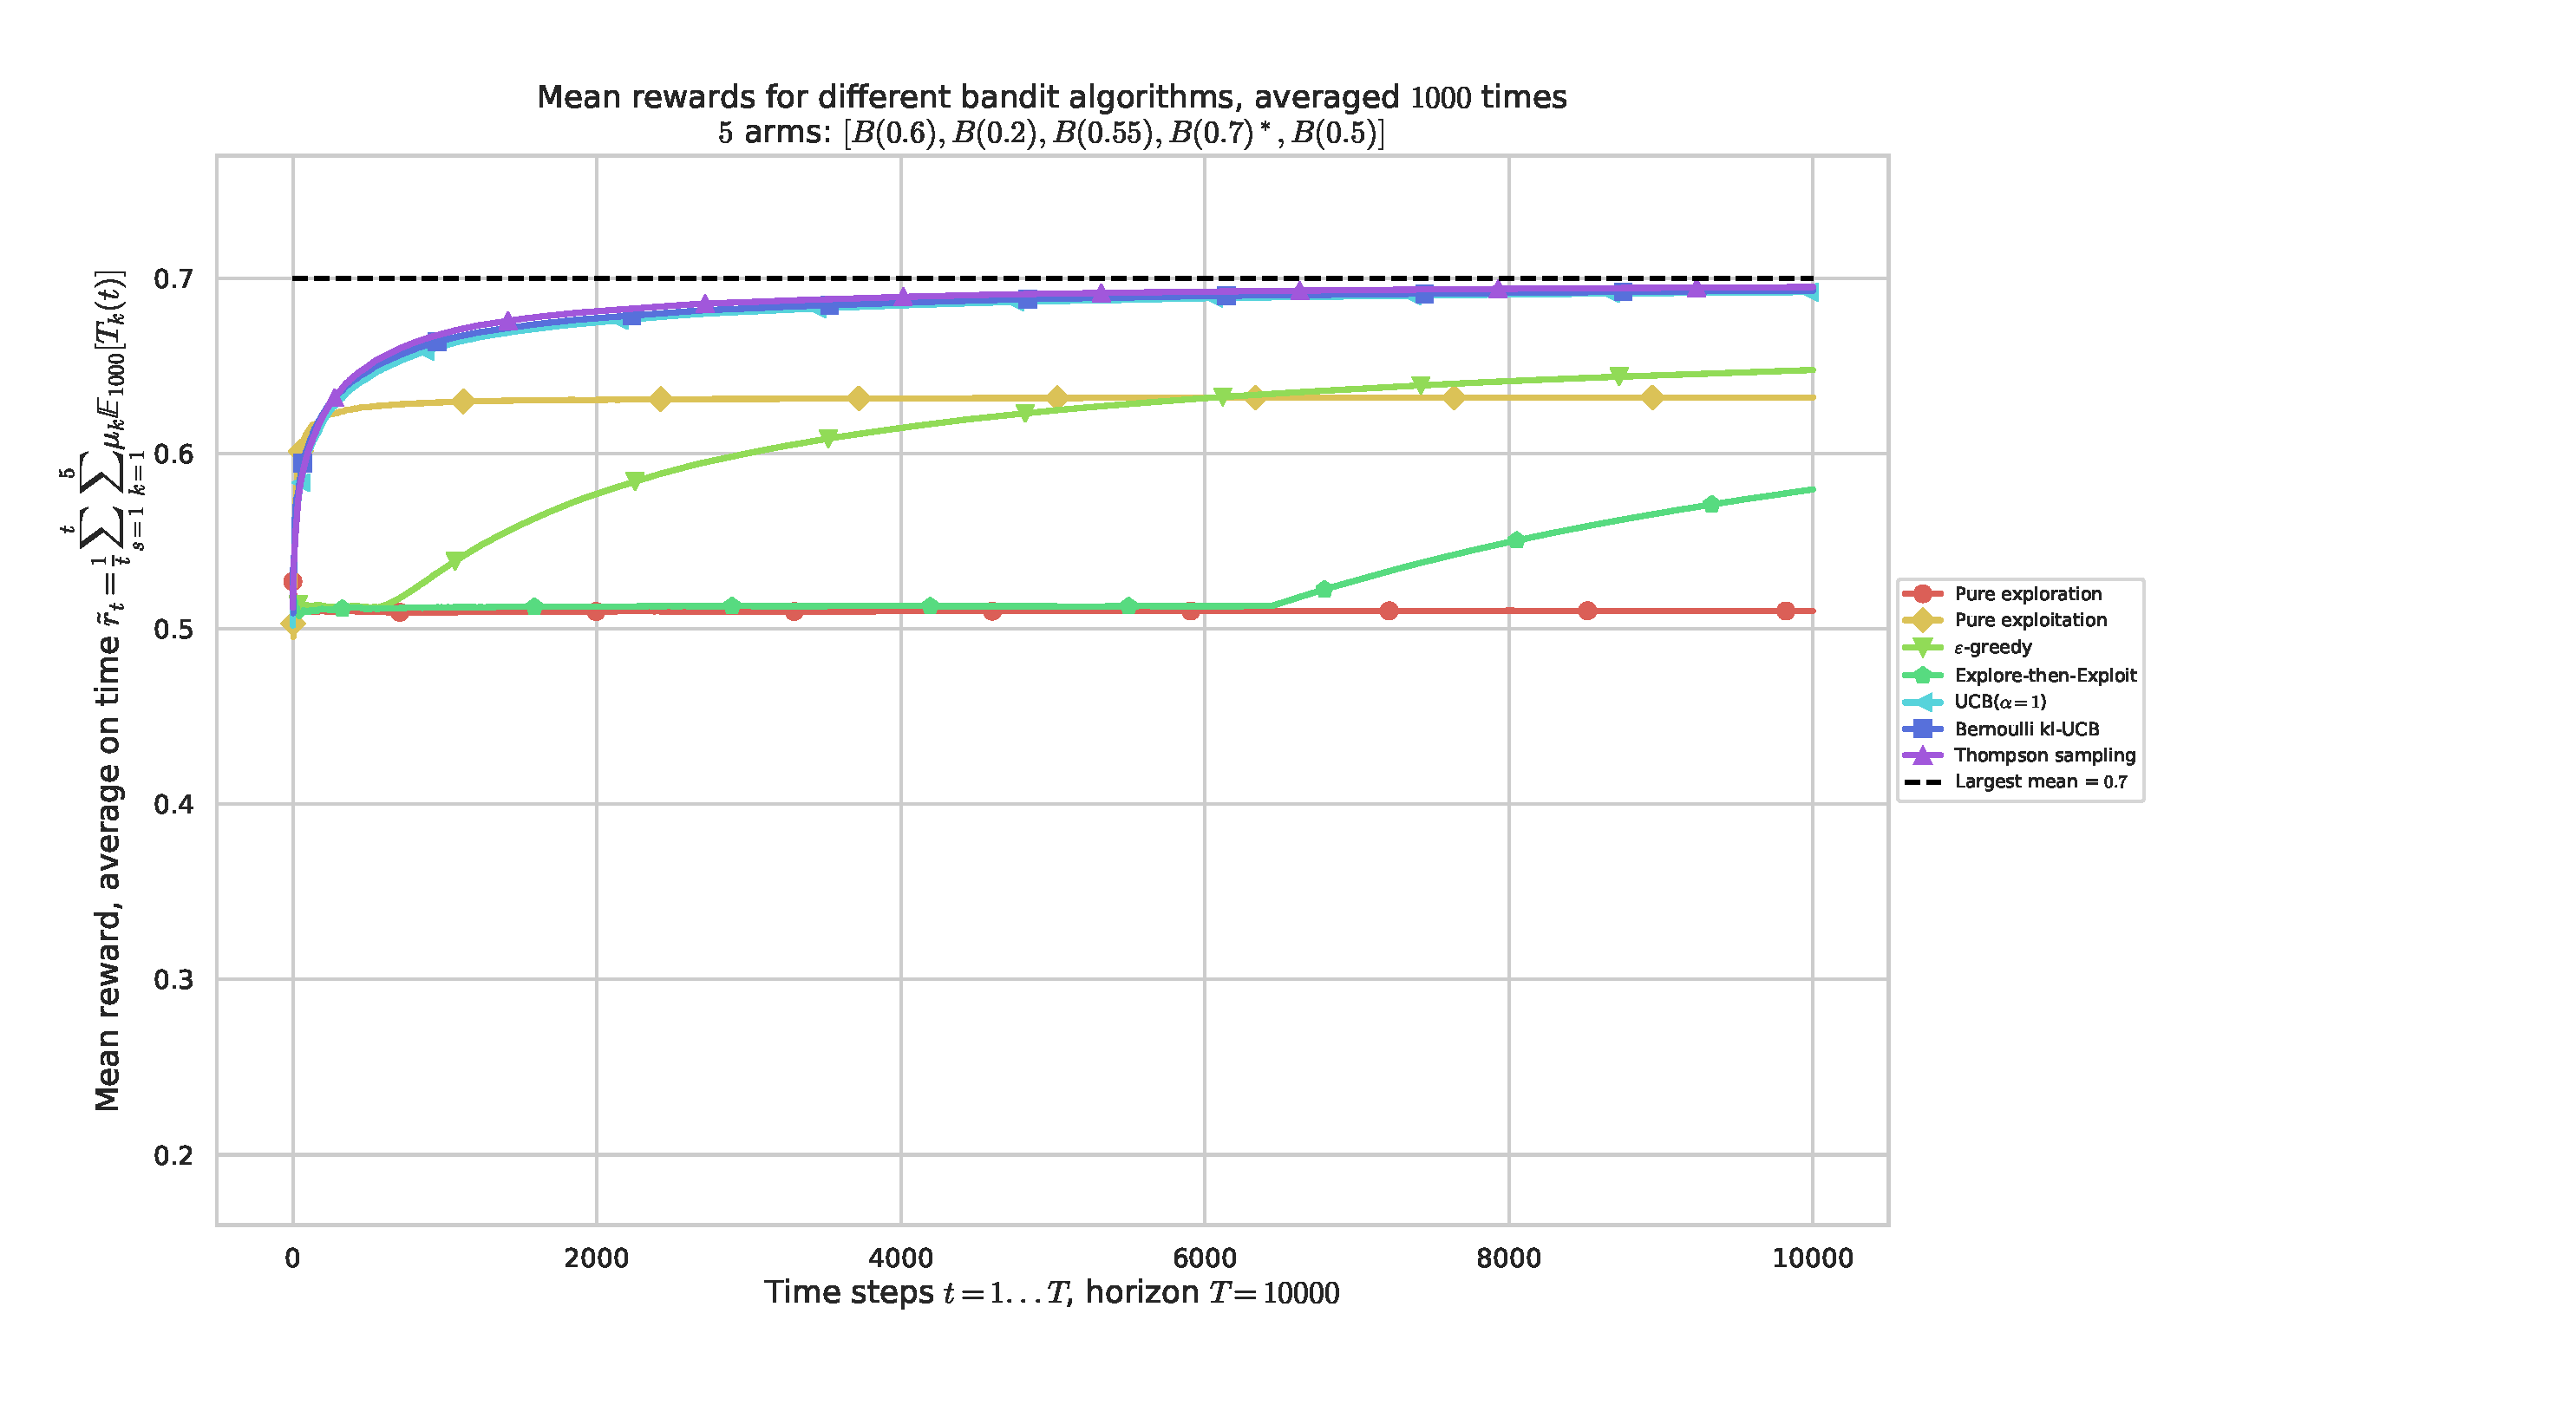
\includegraphics[width=1.14\linewidth]{SP__K5_T10000_N1000__7_algos/main_MeanRewards____env1-1_2506036032481767447.pdf}
	\caption{Average of the cumulated rewards, as function of $t$, for $T=10000$ and $N=1000$.}
	\label{fig:2:meanRewardsAsFunctionOfTimeForDifferentAlgorithmsT10000N1000}
\end{figure}

\begin{figure}[h!]  % [htbp]
	% \centering
	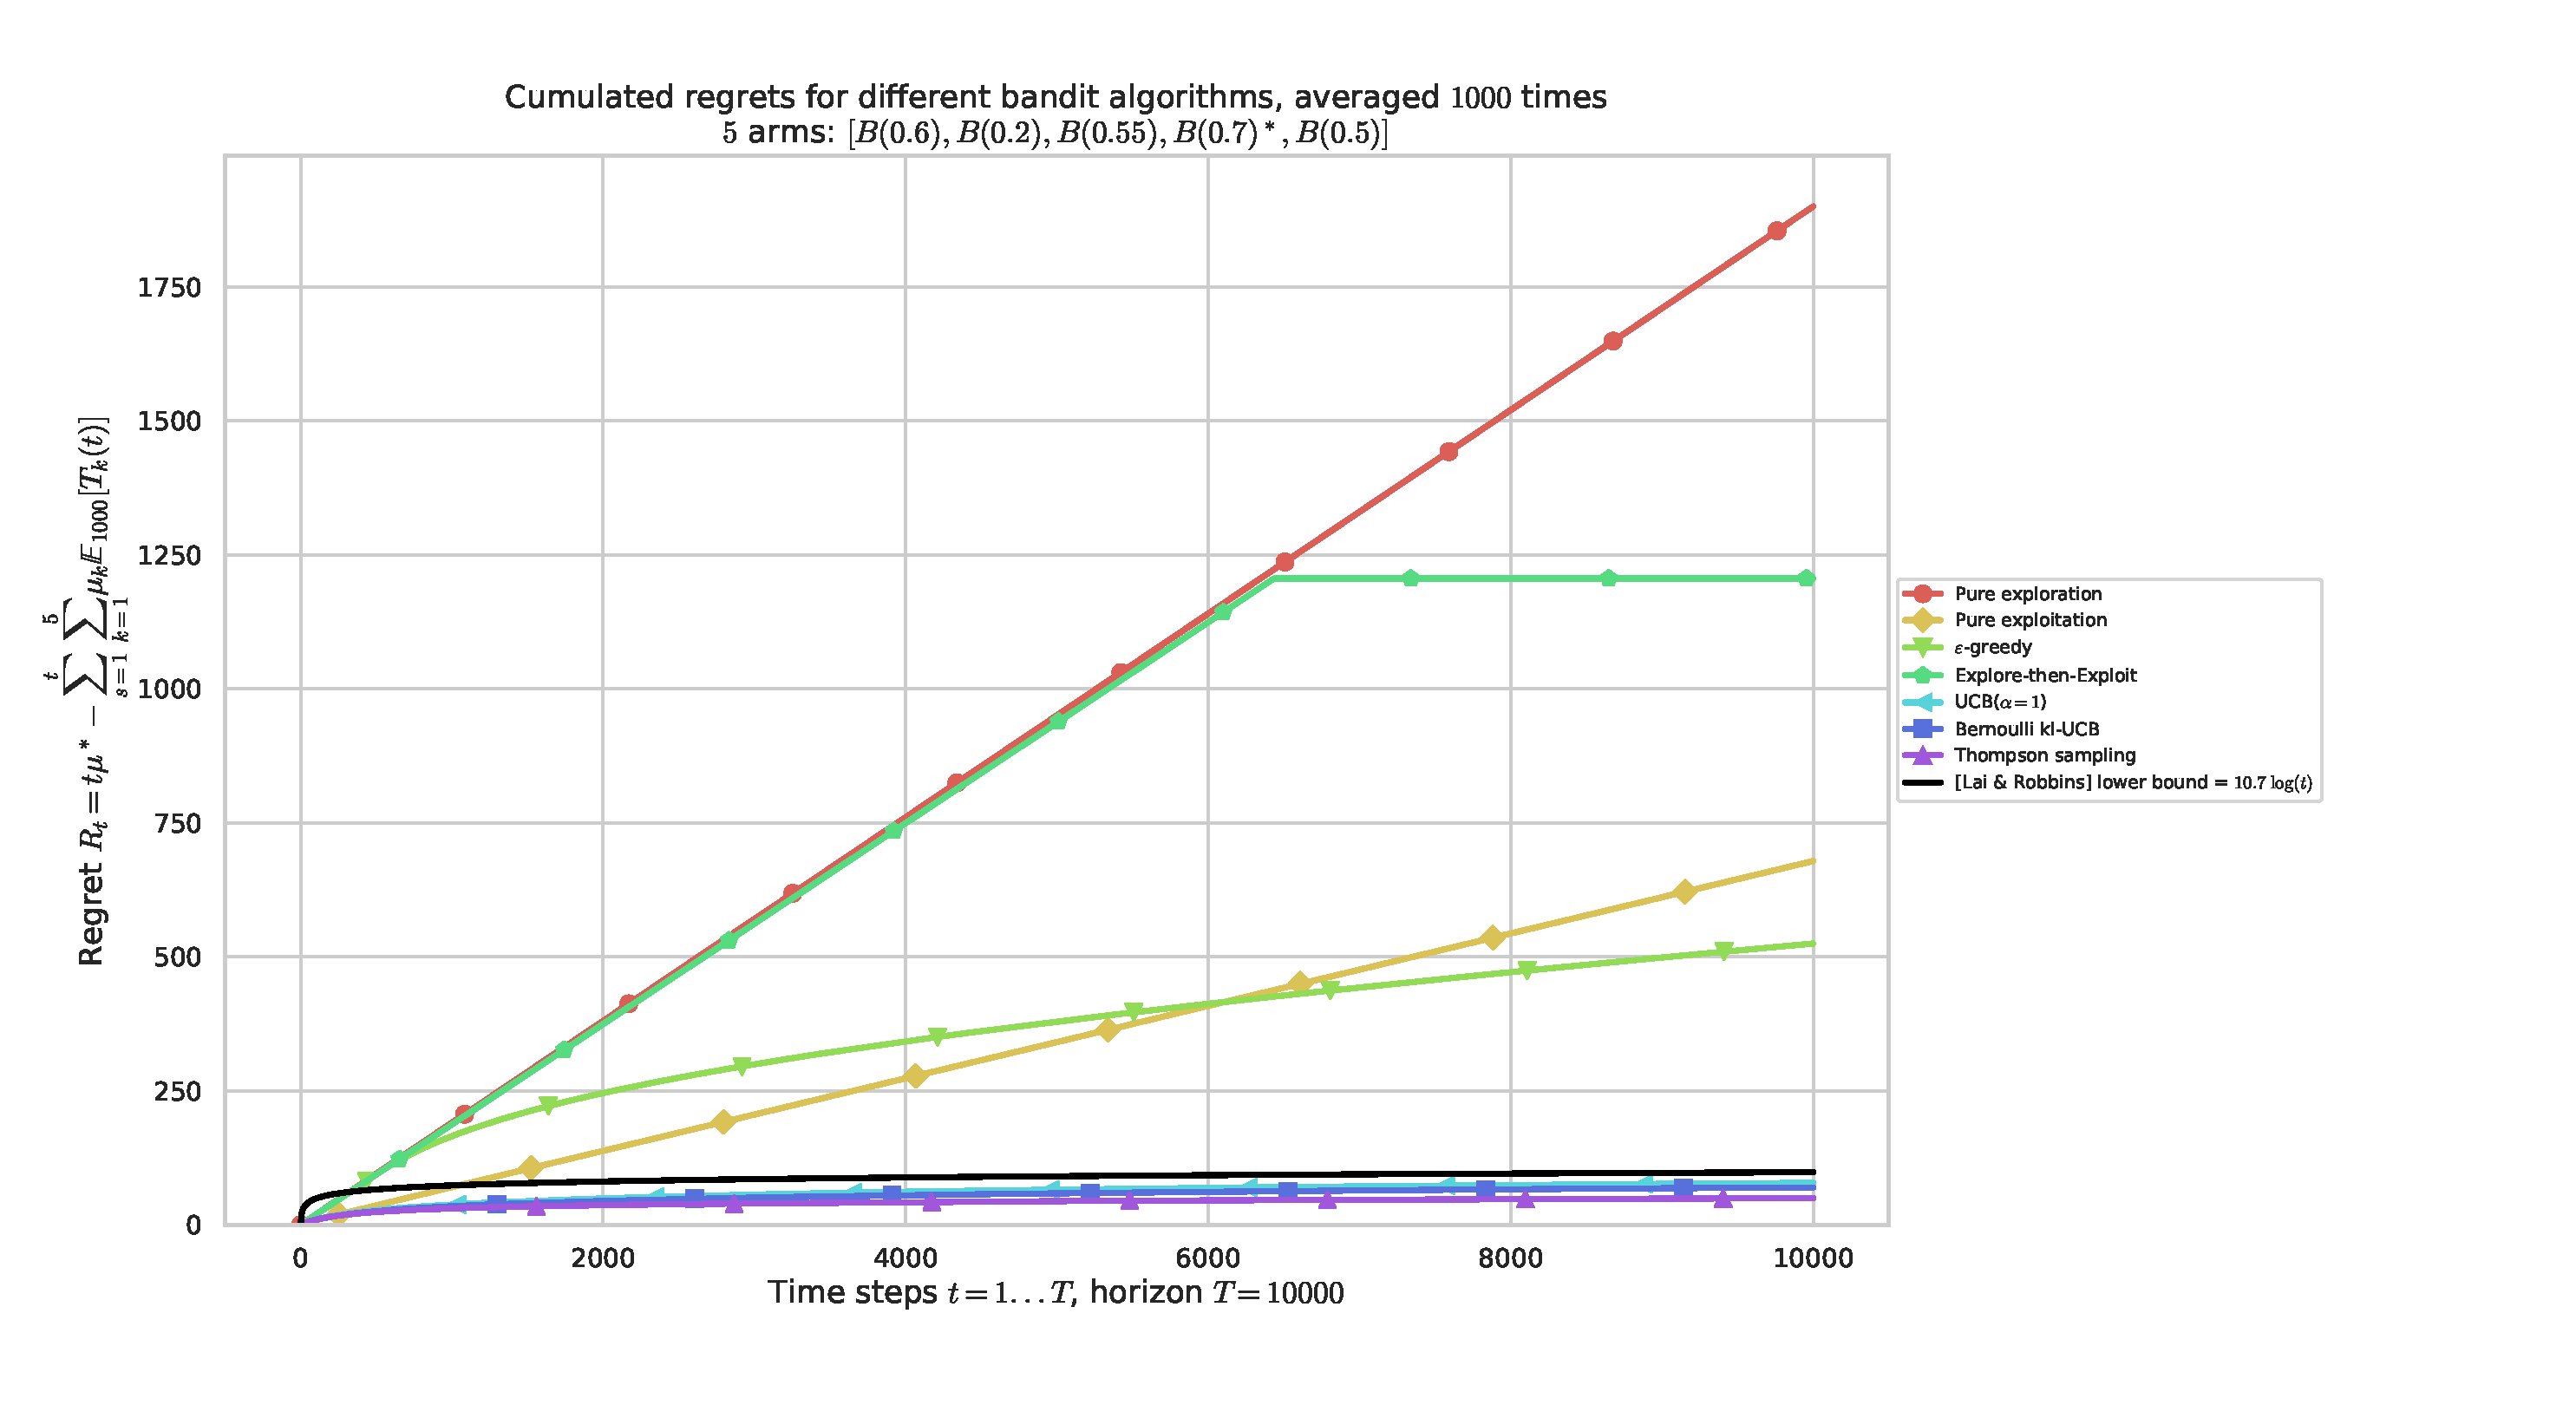
\includegraphics[width=1.14\linewidth]{SP__K5_T10000_N1000__7_algos/main____env1-1_2506036032481767447.pdf}
	\caption{Mean regret $R_t$ as function of $t$ for $T=10000$ and $N=1000$.}
	\label{fig:2:meanRegretAsFunctionOfTimeForDifferentAlgorithmsT10000N1000}
\end{figure}



\paragraph{Summary of this review of MAB algorithms.}
%
We gave an overview of the most well known families of algorithms for multi-armed bandits,
focussing on algorithms designed and analyzed for the single-player stationary and stochastic MAB model.
Except the naive and simple strategies given as introductory examples, most of the policies presented above are order-optimal for Bernoulli distributed problems or bounded rewards (or one-dimensional exponential families),
and some of them are known to be optimal in different settings.
%
To clearly understand the different in their empirical behaviors, we illustrated the performance of two naive and two simple strategies against three efficient ones, on the example of Bernoulli-distributed problem used for the online demonstration from Section~\ref{sec:2:notations} (see Figures~\ref{fig:2:example_of_a_5_arm_bandit_problem} and \ref{fig:2:example_of_a_5_arm_bandit_problem__step100}).
This also serves as a first example of numerical simulation performed with our library SMPyBandits, before the large-scale experiments of Section~\ref{sec:3:reviewSPAlgorithms} below.
%
In the rest of this thesis, we mainly use the $\UCB_1$ or Thompson sampling algorithms when simplicity and realistic deployment is favored (\ie, Chapter~\ref{chapter:4}), and the \klUCB{} algorithm when we give mathematical developments (\ie, Chapters~\ref{chapter:5} and \ref{chapter:6}).


% % \newpage

% % ----------------------------------------------------------------------------
% \section{Different approaches on algorithm selection}
% \label{sec:2:chooseYourPreferredBanditAlgorithm}

% For any real-world applications of MAB algorithms,
% several solutions have been explored based on various models, and for any model, typically there are many algorithms available, as we have seen above.
% %
% Thus, when a practitioner is facing a problem where MAB algorithms could be used, it is not an easy task to decide which algorithm to use.
% It is hard to predict which solution could be the best for real-world conditions at every instant,
% and even by assuming a stationary environment, when one is facing a certain problem but has limited information about it, it is hard to know beforehand which algorithm can be the best solution.

% In this Section, we first present two naive approaches for selecting an algorithm when facing a new problem, and then we detail the online approach that uses a ``leader'' MAB algorithm running on top of a pool of ``followers'' algorithms, and we present our contribution that is a new ``leader'' algorithm based on \ExpQ.
% This section is based on our article \cite{Besson2018WCNC}.


% % ----------------------------------------------------------------------
% \subsection{Motivation for online algorithm selection}\label{sub:25:introduction}

% Many different learning algorithms have been proposed by the machine learning community,
% and most of them depend on several parameters, for instance $\alpha$ for $\UCB_1$, the prior for Thompson sampling or BayesUCB,
% the $\kl$ function for \klUCB{} etc.
% Every time a new MAB algorithm $\Alg$ is introduced, it is compared and benchmarked on some bandit instances, parameterized by $\boldsymbol{\mu} = (\mu_1,\dots,\mu_K)$, usually by focusing on its expected regret $R_T^{\Alg}$.
% %
% For a known and specific instance, simulations help to select the best algorithm in a pool of algorithms,
% but when one wants to tackle an \emph{unknown} real-world problem, one expects to be efficient against \emph{any} problem, of any size and complexity in a certain family:
% ideally one would like to use an algorithm that can be applied identically against any problem of such family.


% \textbf{Naive approaches:}
% %
% On the one hand, a practitioner can decide to pick one algorithm, maybe because it seems efficient on other problems, or maybe because it is simple enough to be used in its application. It might be unrealistic to implement complicated algorithms on limited hardware such as embedded chips in a very low-cost IoT end-device, and for instance a practitioner could chose to only consider the $\UCB_1$ algorithm (or other low-cost algorithms).
% %
% On the other hand, if prior knowledge on the application at hand is available, one could implement some benchmarks, and compare a set of algorithms on different problems. If a leader appears clearly, it is then possible to choose it for the application.


% \textbf{Illustrative example:}
% %
% For instance, if you know that the considered problem can either have $K$ arms with very close means, or one optimal arm far away from the other, two versions of $\UCB_1$ will perform quite differently in the two problems:
% using a large $\alpha$, \ie, favoring exploration, will give low regret in the first case,
% while using a low $\alpha$, \ie, favoring exploitation, will give low regret in the second case.
% One approach can be to use an intermediate value, as $\alpha=1/2$ suggested by theory, but another approach could be to consider an aggregated vote of different versions of $\UCB_1$, each running with a different value of $\alpha$ (\eg, in a logarithmic grid), and let another learning algorithm decide which value of $\alpha$ is the best \emph{for the problem at hand}.

% \textbf{The online approach:}
% %
% Another possibility is to consider an online approach, which is interested in the case where the computation power or memory storage of the application is not a limitation factor, but where one cannot run benchmarks before deploying the application.
% We consider a fixed set of algorithms, and we use another learning algorithm on top of this set, to learn \emph{on the fly} which one should be trusted more, and eventually, used on its own.

% The aggregation approach is especially interesting if we know that the problem the application will face is one of a few known kinds of problems.
% In such cases, if there are $N$ different sorts of problems, and if the practitioner has prior knowledge on it, one can use the naive approach to select an algorithm $\cA_i$ which should perform well on problem $i$, for $i\in[N]$,
% and use the aggregation of $\cA_1,\dots,\cA_N$ when facing the unknown problem.

% % To choose the best algorithm, three approaches can be followed:
% % \begin{itemize}
% %     \item
% % \end{itemize}
% % either extensive benchmarks are done beforehand -- if this is possible -- to select the algorithm and its optimal parameters, or an adaptive algorithm is used to learn \emph{on the fly} its parameters.

% % We present a simple adaptive solution, that aggregates several learning algorithms in parallel and adaptively chooses which one to trust the most.

% % \paragraph{Outline.}
% % This section is organized as follows.
% % First, we explain in Section~\ref{sub:25:aggregation} how to combine such algorithms for aggregation.
% % Then we present our proposed algorithm, called \Aggr, in Section~\ref{sub:25:Aggr},
% % Finally, we present numerical experiments in Section~\ref{sub:25:numExp},
% % on Bernoulli and non-Bernoulli MAB problems,
% % comparing the regret of several algorithms against different aggregation algorithms.
% % Theoretical guarantees are shortly discussed in Section~\ref{sub:25:theory}, and Section~\ref{sub:25:conclusion} concludes.


% % \subsection{Naive approaches}

% % As mentioned, there are two naive approaches

% % use UCB or Thompson sampling, and forget about the rest!}
% % First solution: be naive, only use UCB everywhere


% % \subsection{Use prior knowledge about the future application to select beforehand the chosen algorithm}

% % Second solution, if one has some prior knowledge about the domain or setting for which the learning algorithms will be deployed, she can run synthetic or real-world simulations, compare many algorithms before deployment, and select the best algorithm!


% \subsection{Online algorithm selection with expert aggregation}

% % - ``Aggregation of Multi-Armed Bandits learning algorithms for Opportunistic Spectrum Access'', see https://hal.inria.fr/hal-01705292

As we said, a third possible approach is to select \emph{on the run} the best algorithm for a specific situation, for which the so called \emph{expert aggregation algorithms} framework can be useful.
%
To the best of our knowledge, aggregation algorithms, such as \ExpQ{} which dates back from 2002 \cite{Auer02},
have never been used in pratice for stochastic MAB problems.
% and we show that it appears empirically sub-optimal when applied to simple stochastic problems.

We present an improved variant of \ExpQ, called \Aggr.
For synthetic MAB problems, with Bernoulli or other distributions for $K$ arms, simulation results are presented to demonstrate its empirical efficiency.
We combine classical algorithms, such as Thompson sampling, Upper-Confidence Bounds algorithms (\UCB{} and variants), and Bayesian or Kullback-Leibler UCB.
%
Our algorithm offers good performance compared to state-of-the-art algorithms
(\ExpQ{}, \CORRAL{} or \LearnExp{}) \cite{Agarwal16,Singla17},
and appears as a robust approach to select on the run the best algorithm for any stochastic MAB problem, being more realistic to real-world radio settings than any tuning-based approach.

% \TODOL{This chapter is basically a raw include from my paper ``Aggregation of Multi-Armed Bandits learning algorithms for Opportunistic Spectrum Access'', see https://hal.inria.fr/hal-01705292}


% ----------------------------------------------------------------------
% \subsection{Aggregating bandit algorithms}\label{sub:25:aggregation}
\paragraph{Notations}\label{sub:25:aggregation}

We assume to have $N \geq 2$ MAB algorithms, $\Alg_1, \dots, \Alg_N$,
and let $\Alg_{\mathrm{aggr}}$ be an aggregation algorithm,
which runs the $N$ algorithms in parallel (with the same slotted time), and use them to choose its channels based on a voting from their $N$ decisions.
%
$\Alg_{\mathrm{aggr}}$ depends on a pool of algorithms and a set of parameters.
We would like that $\Alg_{\mathrm{aggr}}$
performs almost as well as the best of the $\Alg_a$, with a good choice of its parameters, independently of the MAB problem.
Ideally $\Alg_{\mathrm{aggr}}$ should perform similarly to the best of the $\Alg_a$.
%
To simplify the presentation, we only aggregate bandit algorithms that give deterministic recommendations:
one arm is chosen with probability $1$ and the others with probability $0$.
However, both \ExpQ{} and \Aggr{} can be adapted to aggregate randomized bandit algorithms, \ie, algorithms that output a probability distribution $\xi_t$ over the arms $[K]$ at each time step, and draw the next selected arm according to this distribution
(\eg, Thompson sampling).

The aggregation algorithm maintains a probability distribution $\pi^{t}$ on the $N$ algorithms $\Alg_a$, starting from a uniform distribution:
$\pi^t_a$ is the probability of trusting the decision made by algorithm $\Alg_a$ at time $t$.
$\Alg_{\mathrm{aggr}}$ then simply performs a weighted vote on its algorithms: it decides whom to trust by sampling $a \in [N]$ from $\pi^t$, then follows $\Alg_a$'s decision.
The main questions are then to know what observations (\ie, arms and rewards) should be given as feedback to which algorithms,
and how to update the trusts at each step, and our proposal \Aggr{} differs from \ExpQ{} on these very points.


% ----------------------------------------------------------------------
\subsection{Our contribution: the \Aggr{} algorithm}\label{sub:25:Aggr}

Our proposed \Aggr{} is detailed in Algorithm~\ref{algo:25:Aggr}.
%
\begin{small}
	\begin{figure}[h!]
		\centering
		\begin{framed}
		% Documentation at http://mirror.ctan.org/tex-archive/macros/latex/contrib/algorithm2e/doc/algorithm2e.pdf if needed
		% Or https://en.wikibooks.org/wiki/LaTeX/Algorithms#Typesetting_using_the_algorithm2e_package
		\begin{algorithm}[H]
			% XXX Input, data and output
			\KwIn{$N$ bandit algorithms, $\Alg_1, \dots, \Alg_N$, with $N \geq 2$}
			\KwIn{Number of arms, $K \geq 2$}
			\KwIn{Time horizon, $T \geq 1$, \textbf{not} used for the learning}
			\KwIn{A sequence of learning rates, $(\eta_t)_{t \geq 1}$}
			\KwData{Initial uniform distribution, $\pi^{0} = \cU([N])$}
			\KwResult{$\Alg_{\mathrm{aggr}}=\Aggr\left[\Alg_1, \dots, \Alg_N\right]$}
			% XXX Algorithm
			\For(\tcp*[f]{At every time step})
            {$t = 1, \dots, T$}{
				%
				% \tcp{First, run each algorithm $\Alg_a$}
				\For(\tcp*[f]{Can be parallel}){$a = 1, \dots, N$}{
					$\Alg_a$ updates its internal state (e.g., \UCB{} indexes)\;
					It chooses $A(t+1)_{a} \in [K]$.
				}
				%
				% \tcp{The more algorithms have chosen arm $j$, the more probable it is to be chosen.}
				Let $p^{t+1}_j := \sum\limits_{a = 1}^{N} \pi^{t}_a \times \mathbbm{1}(\{A(t+1)_{a} = j\}), \;\forall 1\leq j \leq K$\;
				% \tcp*{Sum trusts}
				Then $\Alg_{\mathrm{aggr}}$ chooses arm $A(t+1) \sim p^{t+1}$\;
				% $\P(A(t+1)_{\mathrm{aggr}} = j) = p^{t+1}_j$
				% \tcp*{Sample once}
				%
				Give \emph{original} reward $(A(t+1), 1 - \ell_{A(t+1)}(t+1))$ to \emph{each} $\Alg_a$ (maybe \emph{not} on its chosen arm)\;
				Compute an \emph{unbiased} estimate of the loss of the trusted algorithms,$$ \ell^{t+1} = \ell_{A(t+1)}(t+1) / p^{t+1}_{A(t+1)}\;. $$
				% \tcp{Use bandit feedback to update $\pi^{t}$}
				% \tcp{Finally, use the instantaneous bandit feedback (loss $\ell_{A(t+1),t}$) to update $\pi^{t}$}
				% \For(\tcp*[f]{Can be parallel}){$a = 1, \dots, N$}{
				\For{$a = 1, \dots, N$}{
					% \eIf{$\Alg_a$ was trusted, \ie, $A(t+1)_{a} = A(t+1)$}{
					\If{$\Alg_a$ was trusted, \ie, $A(t+1)_{a} = A(t+1)$}{
						$ \pi^{t+1}_{a} = \exp(\eta_t \ell^{t+1}) \times \pi^{t}_{a} $
						% \tcp*{More trusted}
						}%{
						% $ \pi^{t+1}_{a} = \exp(- \eta_t \ell^{t+1}) \times \pi^{t}_{a} $
						% \tcp*{Less trusted}
					% }
				}
				Renormalize the new $\pi$: $\pi^{t+1} := \pi^{t+1} / \sum_{a=1}^{N} \pi^{t+1}_{a}$.
				% \tcp*{Project it back to $\Delta_N$}
			}
			\caption{Our aggregation algorithm \Aggr.}
			\label{algo:25:Aggr}
		\end{algorithm}
		\end{framed}
	\end{figure}
\end{small}


At every time step, after having observed a loss $\ell_{A(t+1)}(t+1)$ for its chosen action $A(t+1)$,
the algorithm updates the trust probabilities from $\pi^t$ to $\pi^{t+1}$ by
a multiplicative exponential factor (using the learning rate and the \emph{unbiased} loss).
%
Only the algorithms $\Alg_a$ who advised the last decision get their trust updated, in order to trust more the ``reliable'' algorithms.

The loss estimate is unbiased in the following sense. If one had access to the rewards $r_k(t+1)$ (or the losses $\ell_k(t+1)$) for all arms $k$, the loss incurred by algorithm $a$ at time $t+1$ would be $\tilde{\ell}_{a,t+1} = \ell_{A_A(t+1)}(t+1)$. This quantity can only be observed for those algorithms for which $A_{a}^{t+1}=A(t+1)$. However, by dividing by the probability of observing this recommendation, one obtains an unbiased estimate of $\tilde{\ell}_{a,t}$. More precisely, if we define the estimate by
\begin{equation}
	\hat{\ell}_{a,t+1} = \frac{\ell_{A_A(t+1)}(t+1)}{p_{A_A(t+1)}^{t+1}} \mathbbm{1}(A_A(t+1) = A(t+1))
\end{equation}
satisfies $\mathbb{E}[\hat{\ell}_{a,t+1} | \mathcal{H}_t] = \tilde{\ell}_{a,t+1}$, for all $a$, where the expectation is taken conditionally to the history of observations up to round $t$, $\mathcal{H}_{t}$. Observe that $\tilde{\ell}_{a,t+1}=\ell^{t+1}$ for all algorithms $a$ such that $A_A(t+1)=A(t+1)$, and $\tilde{\ell}_{a,t+1}=0$ otherwise.


% - Precise some tricky points
An important feature of \Aggr{} is the feedback provided to each underlying bandit algorithm, upon the observation of arm $A(t+1)$. Rather than updating only the trusted algorithms (that is the algorithms which would have drawn arm $A(t+1)$) with the observed reward $r_{A(t+1)}(t+1)=1 - \ell_{A(t+1)}(t+1)$,  we found that updating each algorithm with the (original) loss observed for arm $A(t+1)$ improves the performance drastically.
%
As expected, the more feedback they get, the faster the underlying algorithms learn, and the better the aggregation algorithm is.
This intuition is backed up by theory explained in \cite{Maillard11}.


Regarding the update of $\pi^t$, one can note that the trust probabilities are not all updated before the normalization step,
and an alternative would be to
increase $\pi_{a}$ if $A(t+1)_a = A(t+1)$ and to decrease it otherwise.
It would not be so different, as there is a final renormalization step, and empirically this variation has little impact on the performance of \Aggr{}.



% ----------------------------------------------------------------------
\subsubsection{Explanations of \Aggr{} versus \ExpQ{} }\label{sub:25:Exp4}

% - explain, but don't give pseudo-code ?
The \ExpQ{} algorithm (see, e.g. \cite[Section 4.2]{Bubeck12})
is similar to \Aggr{}, presented in Algorithm \ref{algo:25:Aggr},
but differs in the two following points.
%
First, $a\sim\pi^t$ is sampled first and the arm chosen by $\Alg_a$ is trusted, whereas \Aggr{}
needs to listen to the $N$ decisions to perform the updates on $\pi^{t+1}$.
Then, \ExpQ{} gives back an observation (arm, reward) only to the last trusted algorithm
whereas \Aggr{} gives it to all algorithms.
%
Second, after having computed the loss estimate $\ell$, \ExpQ{} updates the estimated cumulative loss for each algorithm,
$\widetilde{L}_a(t) = \sum_{s=1}^{t} \ell_{A_a^s}(s) \times \mathbbm{1}(A^{s}_{a} = A^{s}_{\mathrm{aggr}})$.
%
Instead
\footnote{~It is the same for constant learning rates, and does not differ much for decreasing learning rates.}
of updating $\pi^{t}$ multiplicatively as we do for our proposal, \ExpQ{} recomputes it, proportionally to
$\exp(- \eta_t \widetilde{L}_a(t))$.


\paragraph{How to choose the learning rates $(\eta_t)$?}
%
The sequence of non-negative learning rates $(\eta_t)_{t \geq 1}$ used by \ExpQ{} can be arbitrary.
It can be constant but should be non-increasing \cite[Theorem 4.2]{Bubeck12}.
% helps to choose a good sequence.
If the horizon $T$ is known (and fixed), the best choice is given by $\eta_t = \eta = 2 \log(N) / (T K)$.
However, for real-world communication problems, it can be considered unrealistic\footnote{~For more discussion on this hypothesis, we refer to Section~1 of our article \cite{Besson2018DoublingTricks}.} to assume a fixed and known time horizon, so we prefer the alternative horizon-free choice%
\footnote{~It is non-increasing, and is obtained by minimizing the upper-bound on the regret derived in \cite[pp48]{Bubeck12}.}
of learning rates,
$\eta_t = \log(N) / (t K)$ suggested by \cite{Bubeck12}.
We compare both approaches empirically, and the second one usually performs better.
We also stick to this choice of $(\eta_t)_{t \geq 1}$ for \Aggr.



% ----------------------------------------------------------------------
\subsection{Experiments on simulated MAB problems}\label{sub:25:numExp}

% \TODOL{Je pense refaire complètement les expériences de ce morceau.

% - C'est un peu bête de montrer des problèmes chelous genre Gaussien et "mixed" quand tout le reste de la thèse s'intéresse vraiment aux Bernoulli.

% - C'est un peu naze de montrer en log-y ou en log-log, alors que le reste de la thèse s'intéresse uniquement à des plots x-y, ou des histogrammes.

% - Pour être plus consistant avec les sections suivantes, je pourrais inclure juste 1/2 courbes de regret, et un tableau de résultats pour d'autres problèmes ?
% }

% - explain the problem studied in the simulation
We focus on \emph{i.i.d.} MAB problems, with $K = 9$ channels\footnote{~Similar behaviors are observed for any not-too-large values of $K$, we tried up-to $K = 100$ and the same results were obtained.}.
For Bernoulli problem, the first one uses $\boldsymbol{\mu}=[0.1,\dots,0.9]$, and is considered as a ``simple'' problem.
The second one is divided in three groups:
2 very bad arms ($\mu = 0.01, 0.02$), 5 average arms ($\mu = 0.3$ to $0.6$) and 3 very good arms ($\mu = 0.78, 0.8, 0.82$), and it is considered as a ``harder'' problem.
The horizon is set to $T = 20000$ (but its value is unknown to all algorithms), and simulations are repeated $1000$ times, to estimate the expected regret.
%
This empirical estimation of the expected regret $R_T$ is plotted below, as a function of $T$, comparing some algorithms $\Alg_1,\dots,\Alg_N$ (for $N=6$), and their aggregation with \Aggr{} (displayed in orange bold),
using the parameter-free learning rate sequence, $\eta_t = \log{N} / (t K)$.

The Lai \& Robbins' logarithmic lower-bound \cite{LaiRobbins85} is also plotted.
It corresponds to the second point \eqref{eq:2:forSecondLogTLowerBound2} in Theorem~\ref{thm:2:secondLogTLowerBound}.
It is crucial to note that the lower-bound is only asymptotic, and as such one should not be surprised to see regret curves smaller than the lower-bound (\eg, for the easier Bernoulli problem in Figure~\ref{fig:25:EasyBernoulli}).

Note that for each of the $1000$ simulations, we choose to generate all the rewards beforehand, \ie, one full matrix $(r_k(t))_{1\leq k \leq K, 1 \leq t \leq T}$ for every repetition, in order to compare the algorithms on the same realizations%
\footnote{Similar plots and similar results are obtained if this choice is not made, but it makes more sense to compare them against the same randomization. Note that this choice is the default in SMPyBandits, but the other possibility is implemented as well, by changing \texttt{cache\_rewards} to \texttt{true} or \texttt{false} in the \texttt{configuration} dictionary. See Section~\ref{sub:3:miniConfigurationFileSMPyBandits} for explanations on this \texttt{configuration.py} file, or the online documentation.}
of the MAB problem.

We compare our \Aggr{} algorithm,
as well as other aggregation algorithms, \ExpQ{} from \cite{Bubeck12},
\CORRAL{} from \cite{Agarwal16} and \LearnExp{} from \cite{Singla17}, all with their default parameters.
%
The aggregated algorithms consist in a naive uniform exploration (to have at least one algorithm with bad performances, \ie, linear regret, but it is not included in the plots),
\UCB{} with $\alpha=1/2$, three \klUCB{} algorithms respectively using Bernoulli, Gaussian and exponential $\kl$ functions, and BayesUCB and Thompson sampling with uniform prior.

Figures~\ref{fig:25:EasyBernoulli} and \ref{fig:25:HarderMixed} are in semilog-$y$ scale, this helps to see that the best algorithms can be an \emph{order of magnitude} more efficient than the worst, and the \Aggr{} performs similarly to the best ones, when the other aggregation algorithms are usually amongst the worst.
Figure~\ref{fig:25:HarderMixed_semilogx} is in semilog-$x$ scale to show that the regret of efficient algorithms are indeed logarithmic.


\begin{figure}[h!]  % [htbp]
	\centering
	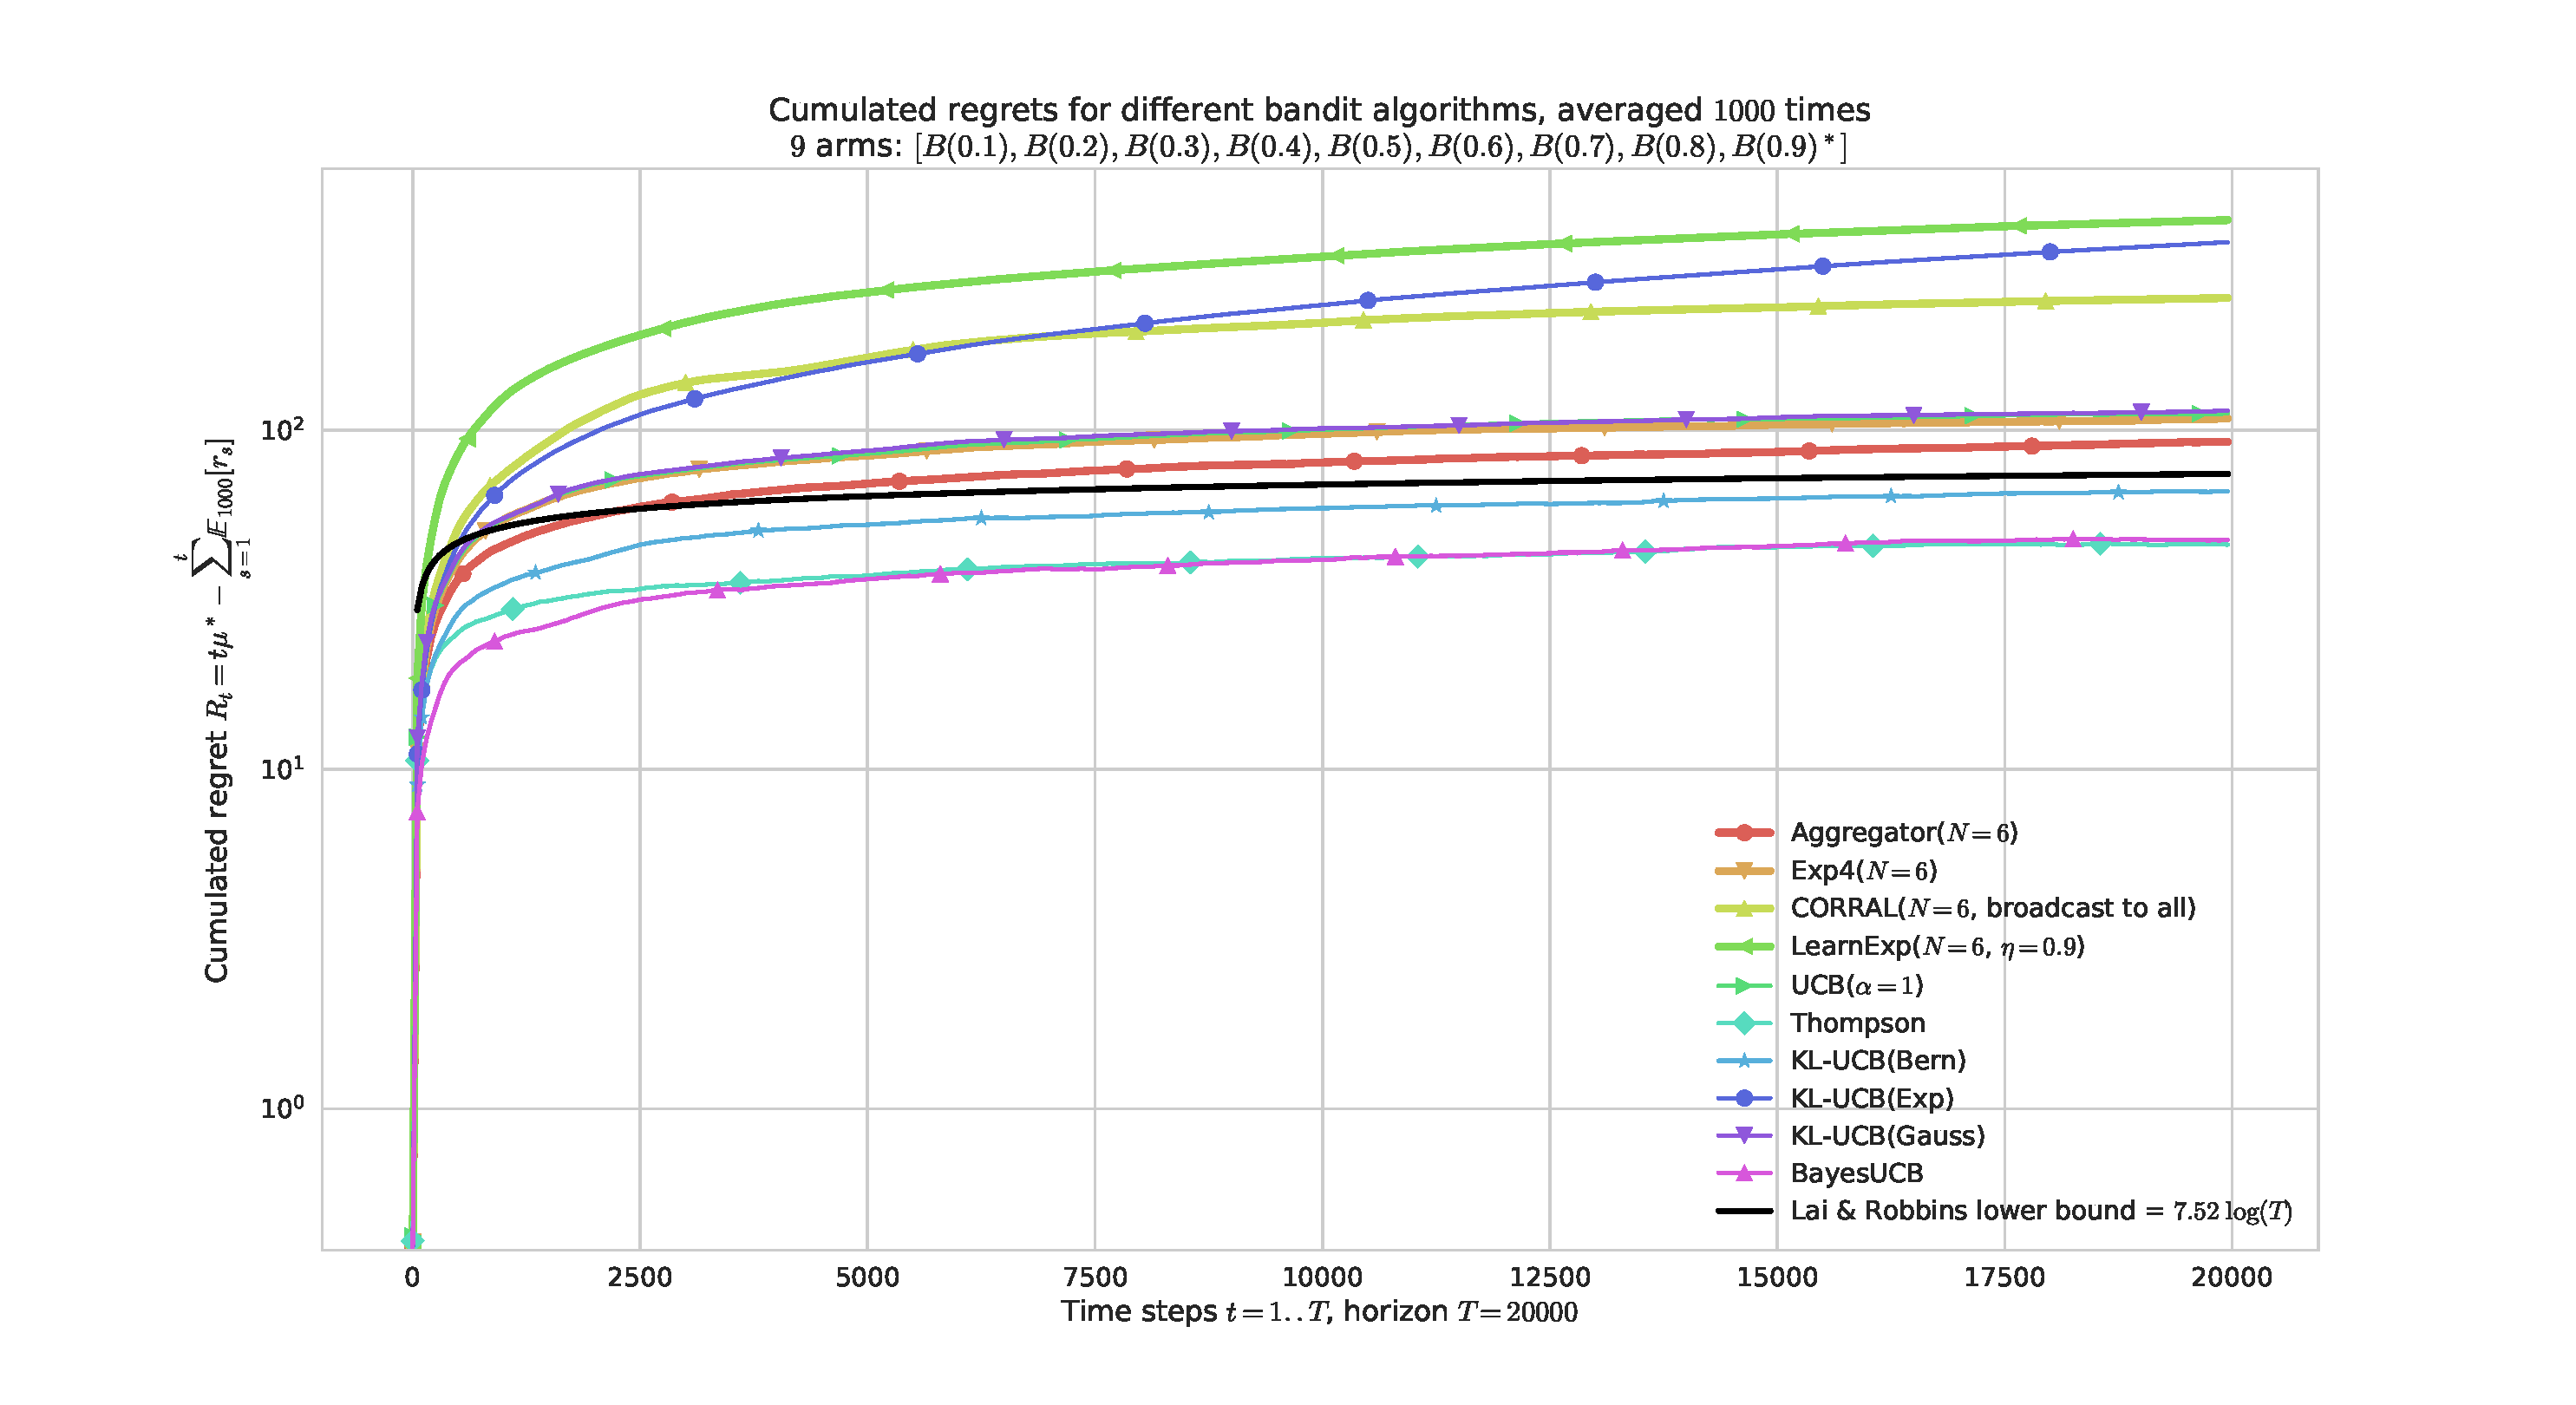
\includegraphics[width=1.10\linewidth]{2-Chapters/2-Chapter/IEEE_WCNC_2018.git/plots/main_semilogy____env1-4_932221613383548446.pdf}
	\caption{On a ``simple'' Bernoulli problem (semilog-$y$ scale).}
	\label{fig:25:EasyBernoulli}
\end{figure}

\begin{figure}[b!]  % [htbp]
	\centering
	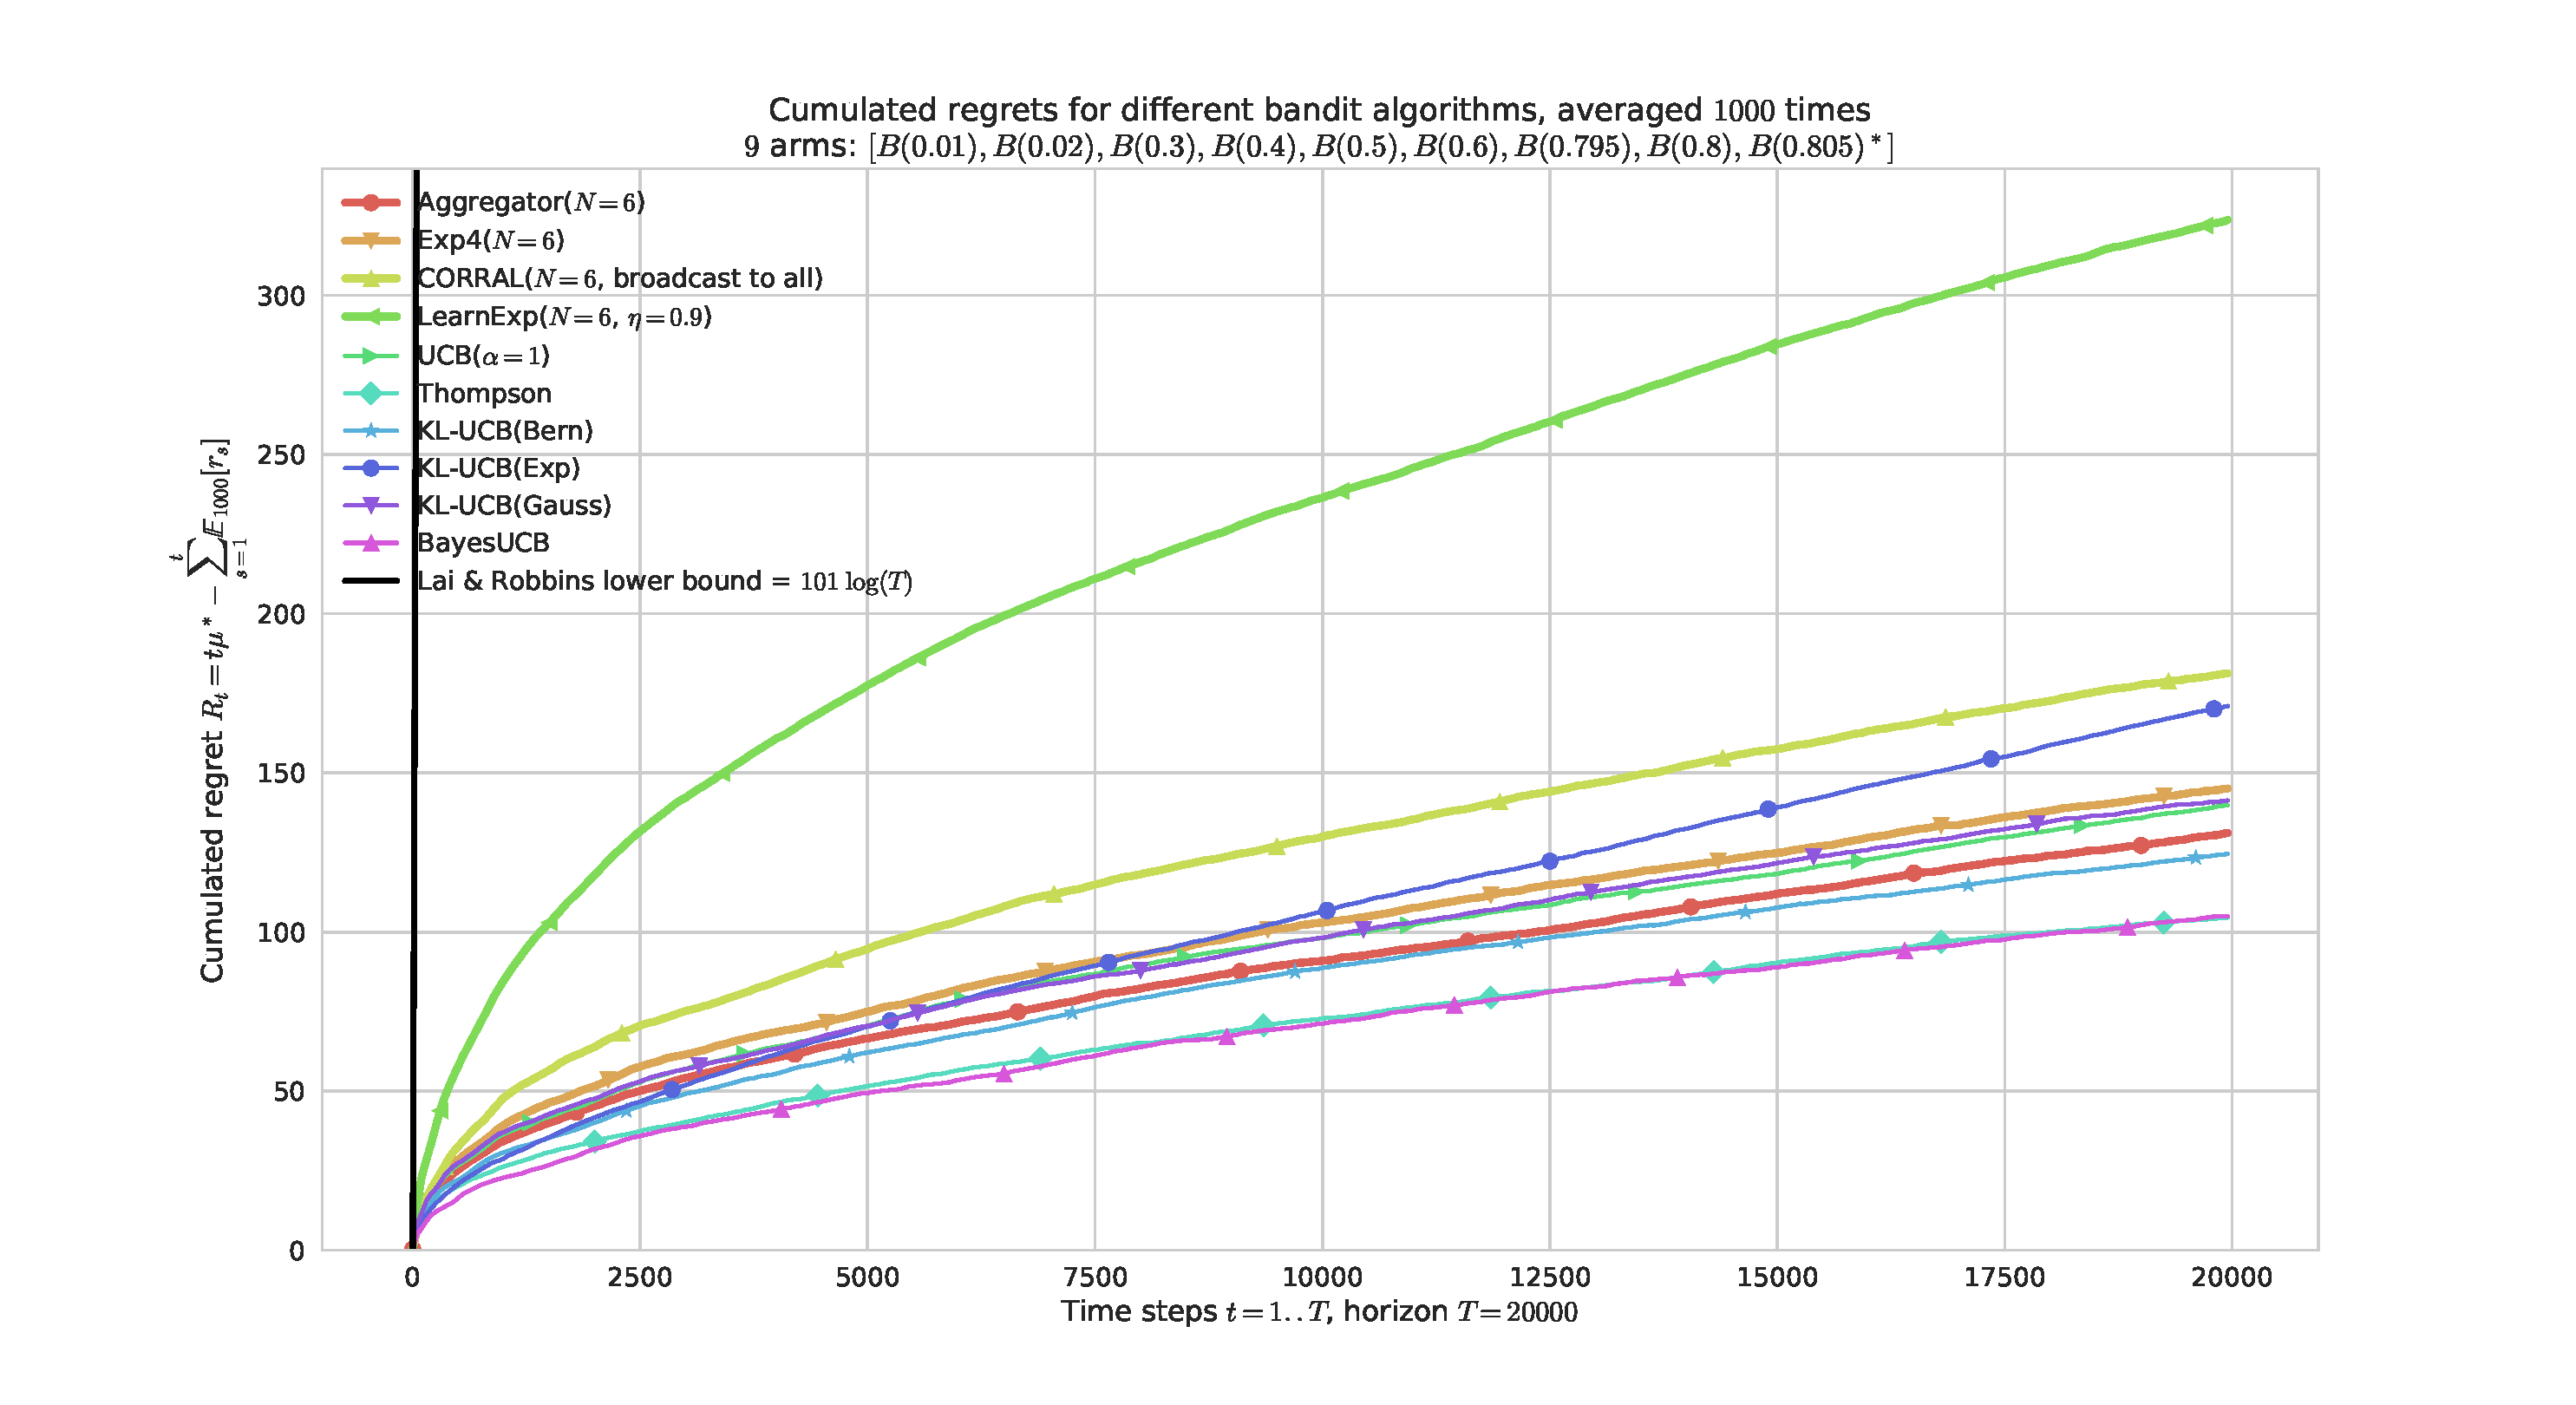
\includegraphics[width=1.10\linewidth]{2-Chapters/2-Chapter/IEEE_WCNC_2018.git/plots/main____env2-4_932221613383548446.pdf}
	\caption{On a ``harder'' Bernoulli problem, they all have similar performances, except \LearnExp.}
	\label{fig:25:HardBernoulli}
\end{figure}

\begin{figure}[b!]  % [htbp]
	\centering
	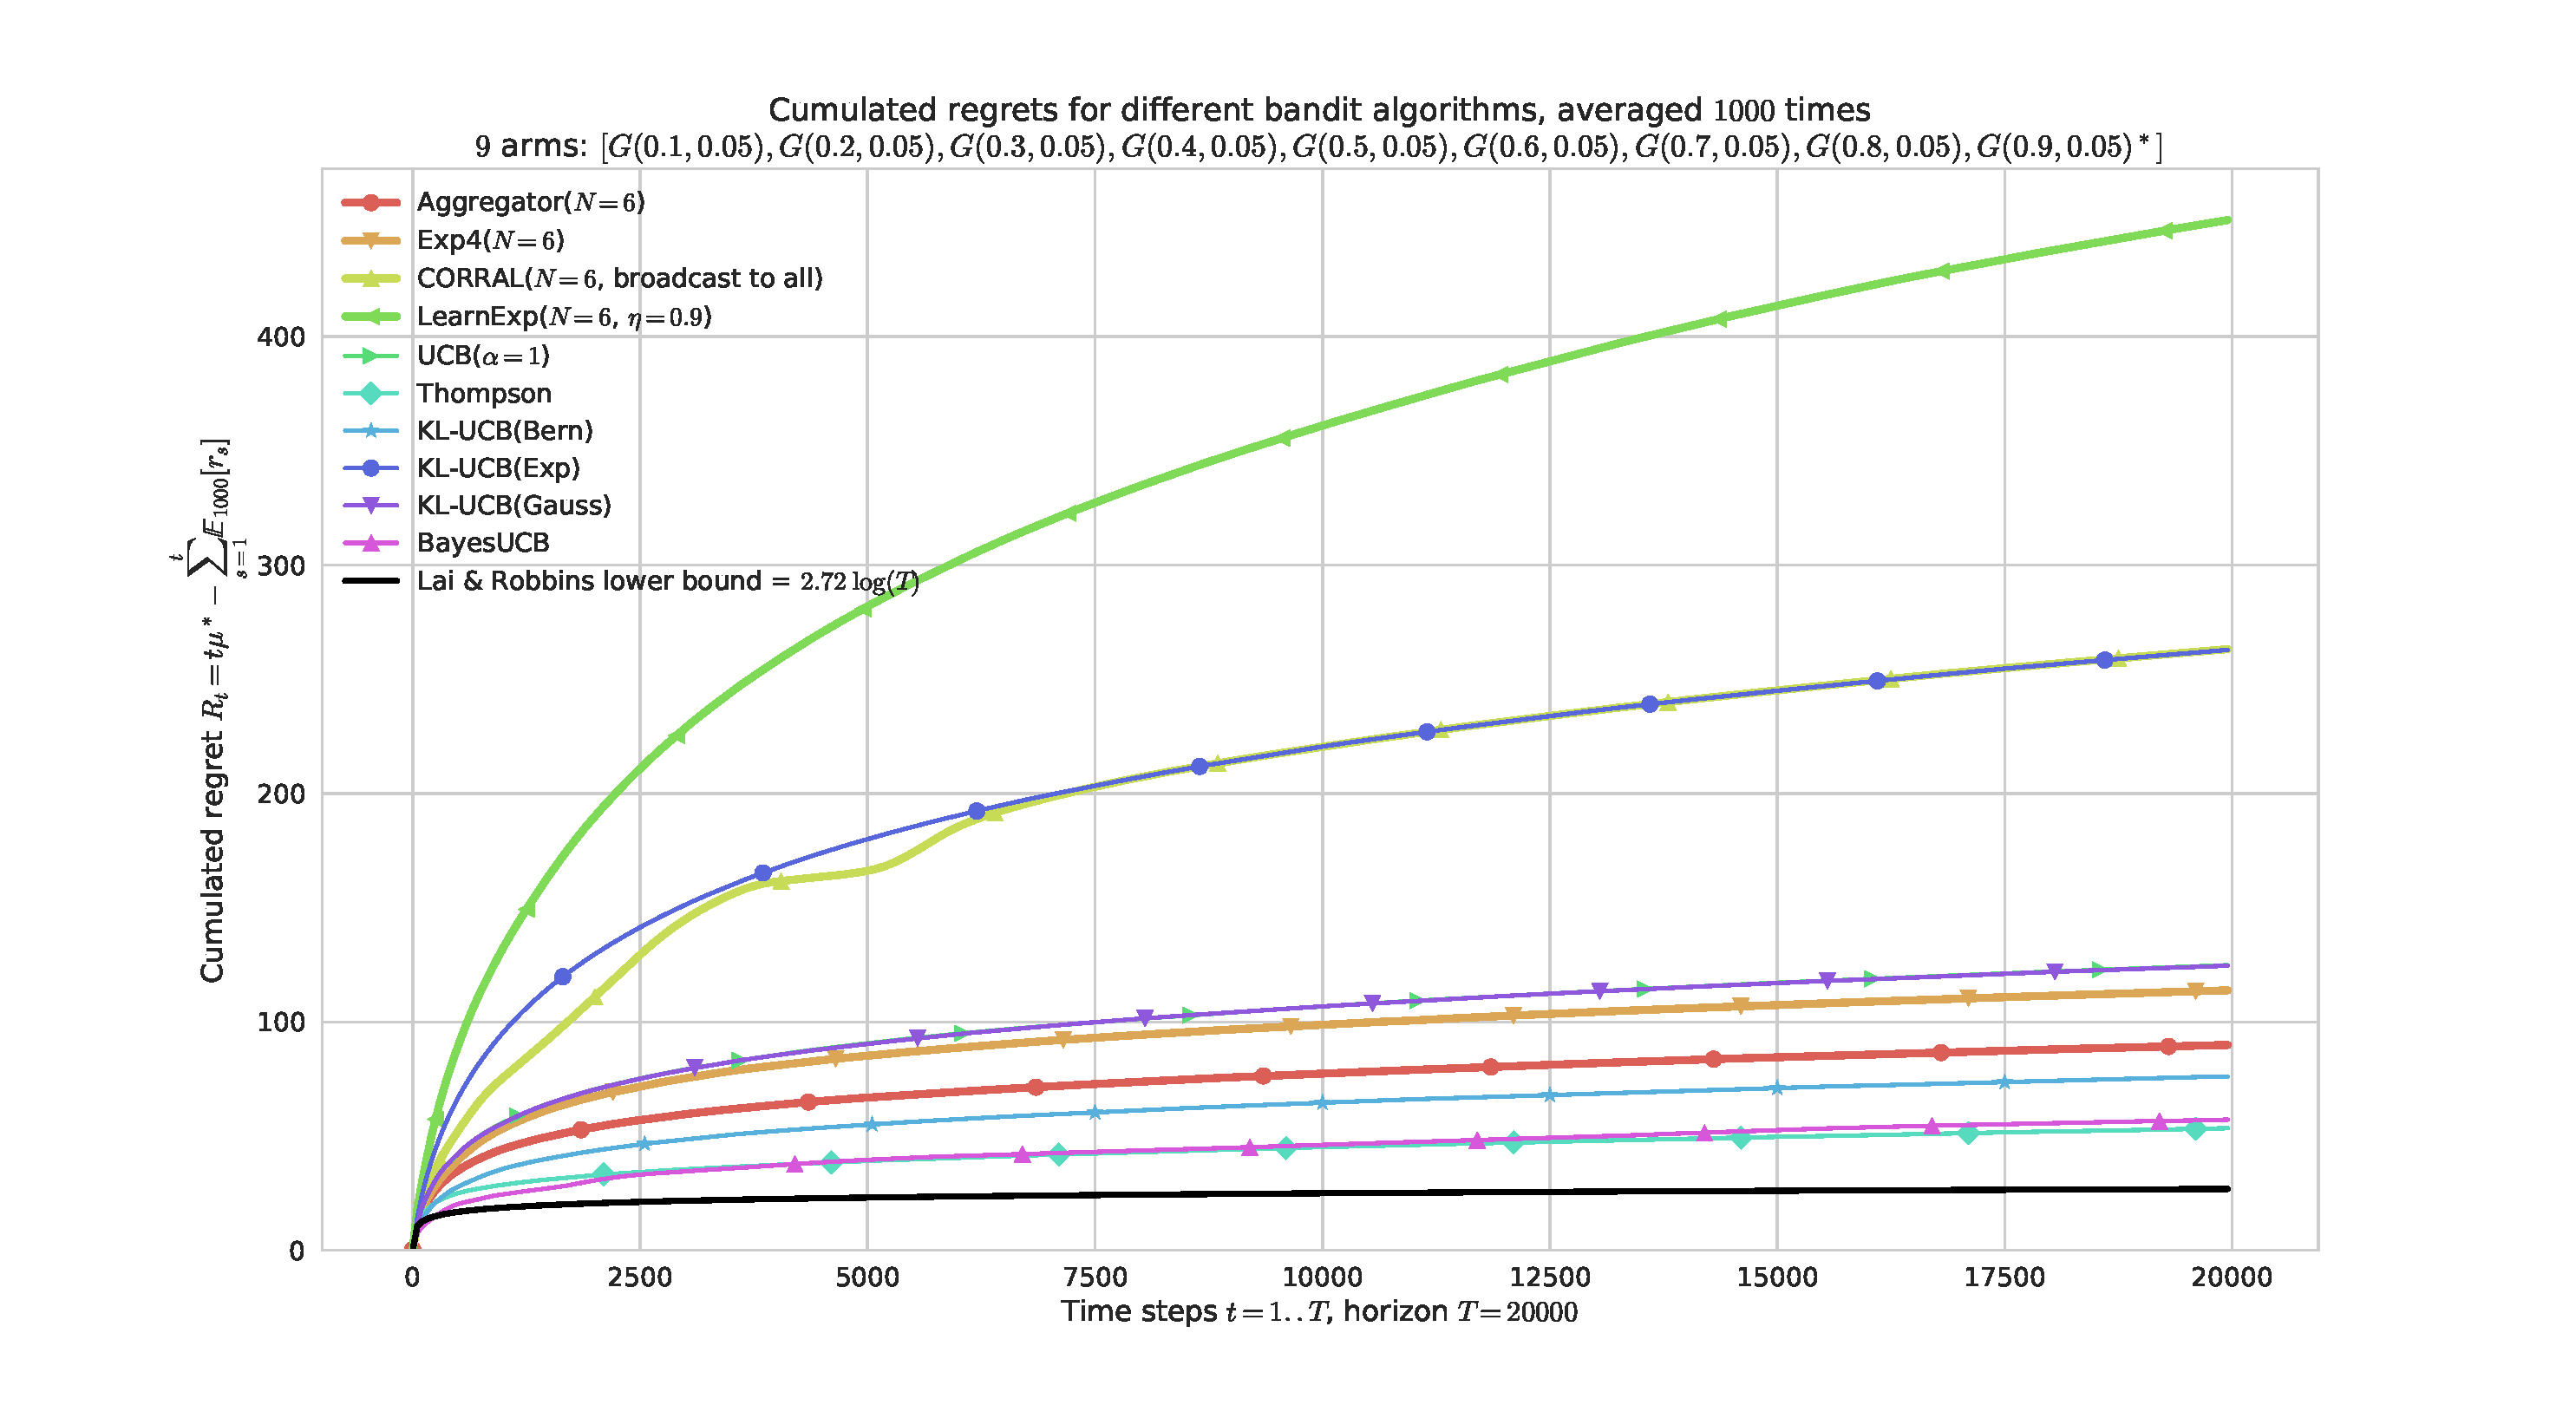
\includegraphics[width=1.10\linewidth]{2-Chapters/2-Chapter/IEEE_WCNC_2018.git/plots/main____env3-4_932221613383548446.pdf}
	\caption{On an ``easy'' Gaussian problem, only \Aggr{} shows reasonable performances, thanks to BayesUCB and Thompson sampling.}
	\label{fig:25:EasyGaussian}
\end{figure}

\begin{figure}[h!]  % [htbp]
	\centering
	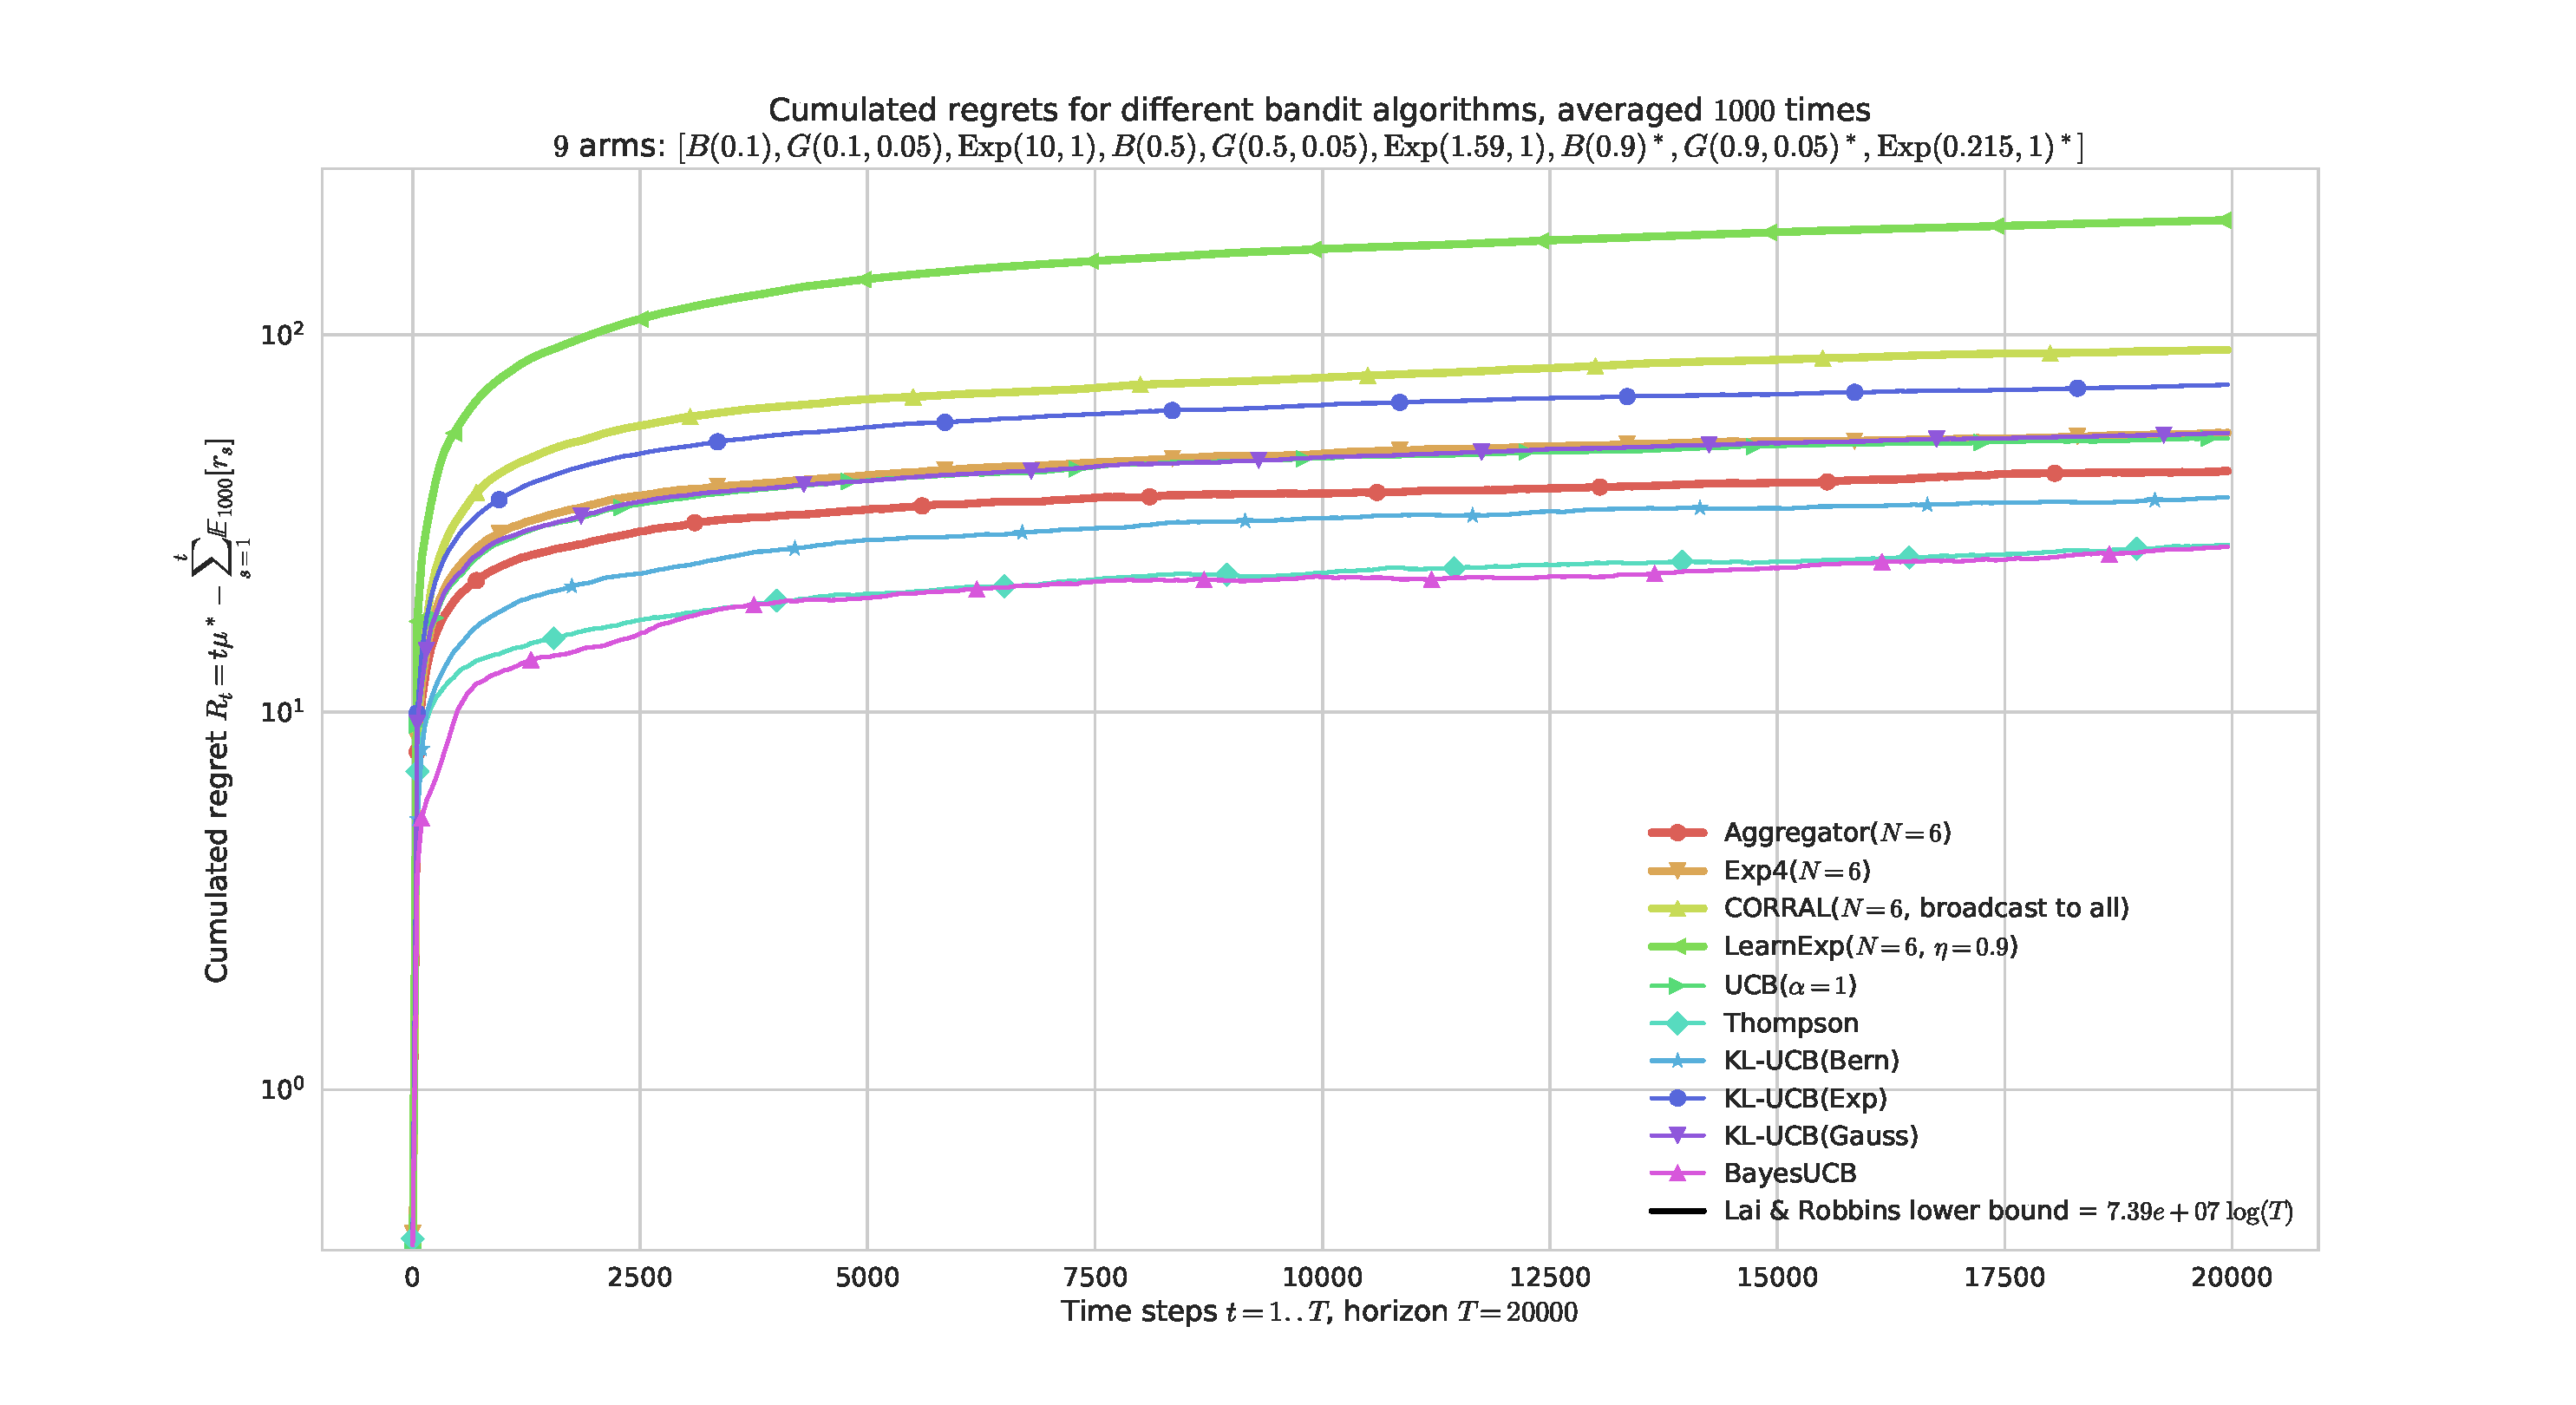
\includegraphics[width=1.10\linewidth]{2-Chapters/2-Chapter/IEEE_WCNC_2018.git/plots/main_semilogy____env4-4_932221613383548446.pdf}
	\caption{On a harder problem, mixing Bernoulli, Gaussian, Exponential arms, with 3 arms of each types with the \emph{same mean}.}
	\label{fig:25:HarderMixed}
\end{figure}

\begin{figure}[b!]  % [htbp]
	\centering
	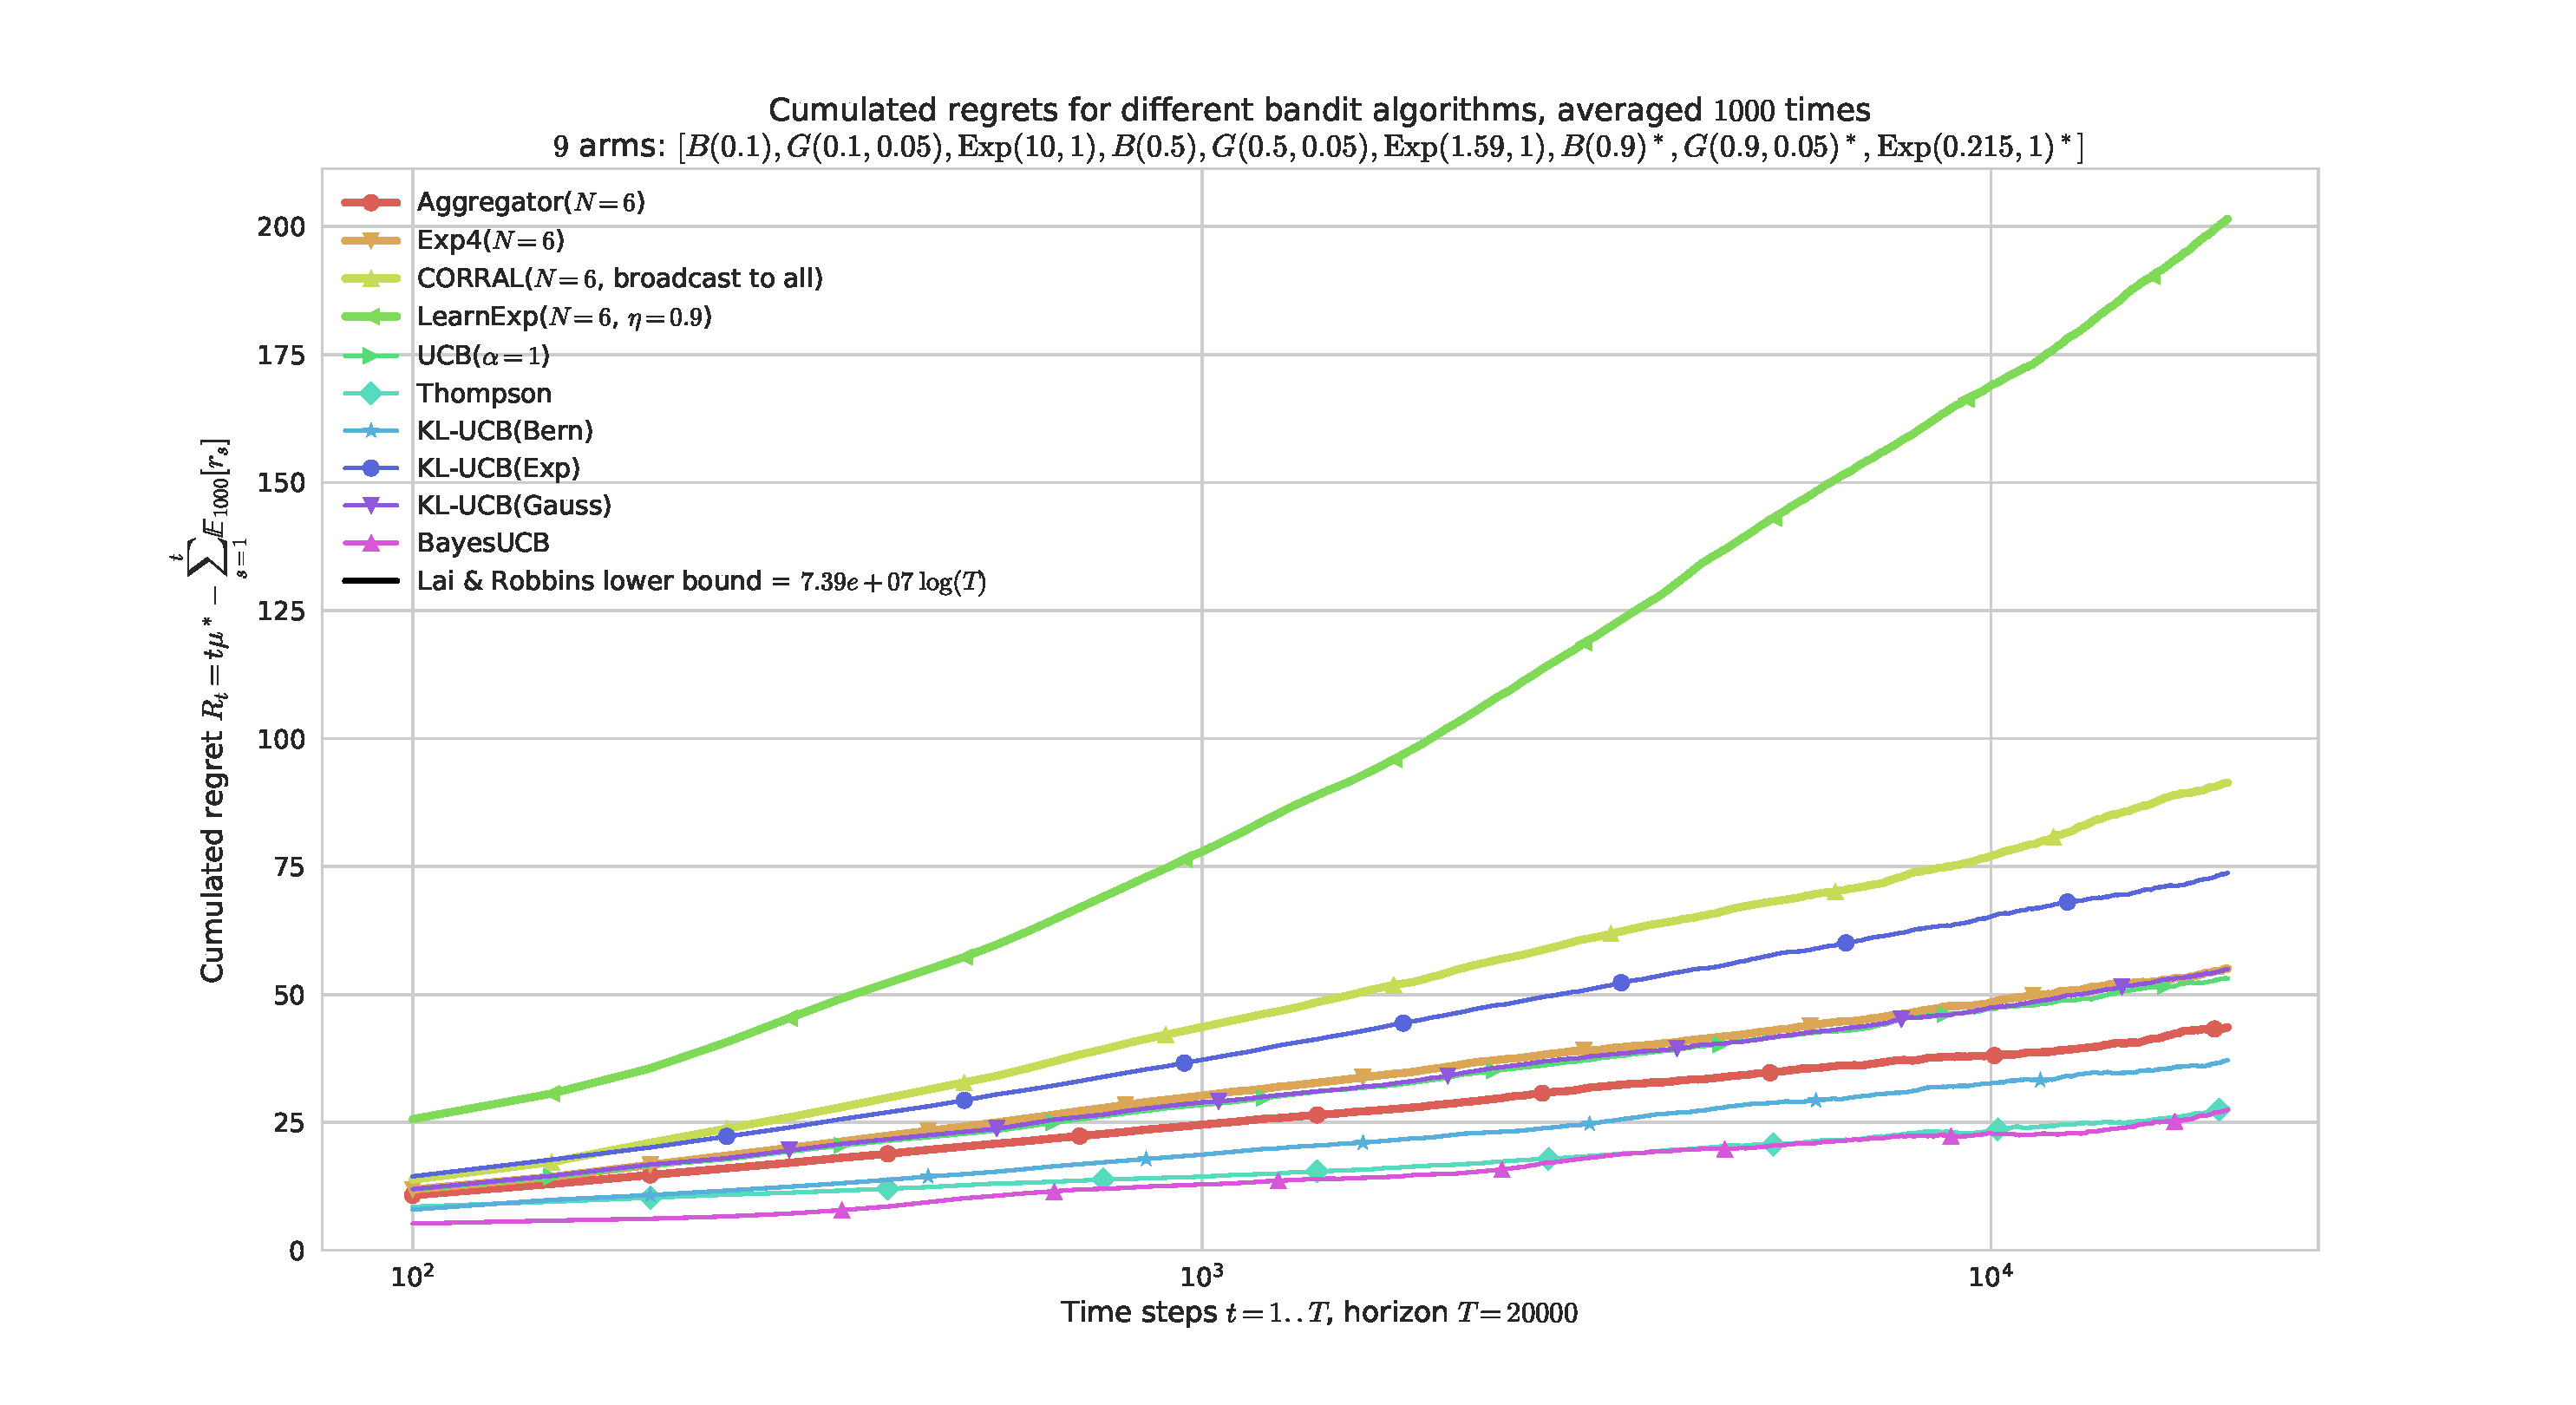
\includegraphics[width=1.10\linewidth]{2-Chapters/2-Chapter/IEEE_WCNC_2018.git/plots/main_semilogx____env4-4_932221613383548446.pdf}
	\caption{The semilog-$x$ scale clearly shows the logarithmic growth of the regret for the best algorithms and our proposal \Aggr, even in a hard ``mixed'' problem (\emph{cf}. Figure~\ref{fig:25:HarderMixed}).}
	\label{fig:25:HarderMixed_semilogx}
\end{figure}

For Bernoulli problems (Figures~\ref{fig:25:EasyBernoulli} and \ref{fig:25:HardBernoulli}), UCB with $\alpha=1/2$, Thompson sampling, BayesUCB and \klUCB{}$^+$ (with the binary $\kl$ function) all perform similarly, and \Aggr{} is found to be as efficient as all of them.
For Gaussian and exponential arms, rewards are truncated into $[0,1]$, and the variance of Gaussian distributions is fixed to $\sigma^2 = 0.05$ for all arms, and can be known to the algorithms (the \kl{} function is adapted to this one-dimensional exponential family).
%
Figure~\ref{fig:25:EasyGaussian} uses only Gaussian arms, with a large gap between their means and a relatively small variance, giving an ``easy'' problem.
%
And Figure~\ref{fig:25:HarderMixed} shows a considerably harder ``mixed'' problem, when the distributions are no longer in the same one-dimensional exponential family and so the Lai \& Robbins' lower-bound no longer holds (even if there still exists a lower-bound).

For each of the 4 problems considered, the \Aggr{} algorithm with default option (broadcast loss to all players) is the best of all the aggregation algorithms,
and its regret is very close to the best of the aggregated algorithms.
Especially in difficult problems with mixed or unknown distributions, \Aggr{} showed to be more efficient that \ExpQ{} and orders of magnitude better than the other reference aggregation algorithms \LearnExp{} and \CORRAL{} (see Figures~\ref{fig:25:HarderMixed} and \ref{fig:25:HarderMixed_semilogx}).


% ----------------------------------------------------------------------
\paragraph{No theoretical guarantees yet}\label{sub:25:theory}

The \Aggr{} does not have satisfying theoretical guarantees in terms of regret $R_T$, unlike many bandit algorithms.
%
Another notion, the \emph{adversarial regret}, denoted by $\overline{R_T}$,
measures the difference in terms of rewards,
between the aggregation algorithm $\Alg_{\mathrm{aggr}}$ and the best aggregated algorithm $\Alg_a$. This is in contrast with the (classical) regret, which measure the difference with the best fixed-arm strategy (Definition~\ref{def:2:regret}).
Thus, even if the aggregated algorithms have logarithmic (classical) regret, having an adversarial regret scaling as $\sqrt{T}$ does not permit to exhibit a logarithmic (classical) regret for the aggregation algorithm.
%
%
Under some additional hypotheses,
\cite[Theorem 4.2]{Bubeck12} proves that
\ExpQ{} satisfies a bound on adversarial regret, % $\overline{R_T}$
$\overline{R_T} \leq 2 \sqrt{T N \log(K)$,
with the good choice of the learning rate sequence $(\eta_t)_{t \geq 1}$.
Our proposed algorithm follows quite closely the architecture of \ExpQ,
and a similar bound for \Aggr{} is expected to hold.
% this is left as a future work.
% For sake of conciseness, we cannot present a proof here.
%

This would be a first theoretical guarantee, but not satisfactory as we saw above that simple algorithms (like \UCB) have regrets scaling as $\log(T)$ \cite{Auer02,Bubeck12}, not $\sqrt{T}$.
%
Regret bounds in several different settings are proved for the \CORRAL{} algorithm \cite{Agarwal16}, but no logarithmic upper-bound can be obtained from their technique, even in the simplest setting of stochastic bandits.
%
However, \Aggr{} always seems to have a (finite-horizon) logarithmic regret in all the experiments we performed,
for both Bernoulli and non-Bernoulli problems (\eg, Gaussian, exponential and Poisson distributions).
Further theoretical developments are left as future work.


% ----------------------------------------------------------------------
\paragraph{Conclusion about our \Aggr{} algorithm}\label{sub:25:conclusion}

We presented the use of aggregation algorithms in the context of Opportunistic Spectrum Access for Cognitive Radio,
especially for the real-world setting of unknown problem instances,
when tuning parameters before-hand is no longer possible and an adaptive algorithm is preferable.
% - \ExpQ and \Aggr works fine
% Both algorithms \ExpQ{} and \Aggr{} have been detailed, and we explained why
Our proposed \Aggr{} was presented in details,
and we also highlighted its differences with \ExpQ.
% as well \color{red} as the intuition that it seems more suited for purely stochastic problems\color{black}.

% - \Aggr{} really help to select the best algorithm against a certain problem, on the fly without any prior knowledge of the problem neither any prior knowledge on which algorithms is the best
We presented experiments on simple MAB problems coming from previous work on bandits for OSA \cite{Jouini10},
and the simulations results showed that \Aggr{} is able to identify on the fly the best algorithm to trust for a specific problem, as expected.
Experiments on problems mixing different families of distributions were also presented, with similar conclusions in favor of \Aggr.
It is not presented in this section, but our proposed algorithm also works well in dynamic scenarios, in which the distribution of the arms can change abruptly at some time,
and appears to be more robust than simple non-aggregated algorithms.

\ExpQ{} has theoretical guarantees in terms of adversarial regret, and even if the same result could hold for \Aggr, results in terms of classical regret are yet to be proved.
Empirically, \Aggr{} showed to always have a logarithmic
regret $R_T$ if it aggregates algorithms with logarithmic regrets (like UCB, \klUCB, Thompson sampling, BayesUCB etc).
It usually succeeds to be close to the best of the aggregated algorithms, both in term of regret and best arm pull frequency.
As expected, the \Aggr{} is never able to outperform any of the aggregated algorithms, but this was an over-optimistic goal.
%
What matters the most is that, empirically, \Aggr{} is able to quickly discover \emph{on the fly} the best algorithms to trust, and then performs almost as well as if it was following it from the beginning.

Our \Aggr{} algorithm could be rewritten as an Online Mirror Descent \cite{Hazan2016introduction,Zimmert2018}, as it is the case for both \ExpQ{} and \CORRAL.
But this direction does not appear very useful, as in the case of \CORRAL{}  the analysis cannot bring a logarithmic regret bound, even by aggregating asymptotically optimal algorithms.
% We will continue investigating regret bounds for \Aggr,
% and other directions include possible applications to the non-stochastic case (\eg, rested or restless Markovian problems, like it was very recently studied in \cite{Luo18}).

\paragraph{Reproducility of the experiments.}
%
Experiments presented in this Section are based on our library SMPyBandits,
and the page \texttt{SMPyBandits.GitHub.io/Aggregation.html} gives instructions to reproduce them.


% ----------------------------------------------------------------------------
% \bibliographystyle{ieeetr}
% \bibliography{IEEE_WCNC__2018__Paper__Lilian_Besson__07-17}


% % A last solution is online algorithm selection, inspired from expert aggregation.
% % Include here the discussion about expert aggregation and my \textbf{Aggregator} algorithm, see https://hal.inria.fr/hal-01705292


\newpage  % WARNING ?

% ----------------------------------------------------------------------------
\section{Conclusion}
\label{sec:2:conclusion}

In this chapter, we presented the multi-armed bandit model, focussing on a finite number of arms, and real-valued rewards.
Our main focus is on one-dimensional exponential families of distributions, and on stochastic and stationary problems.
By showcasing an interactive demonstration made available online,
% XXX ?
% (\href{https://perso.crans.org/besson/phd/MAB\_interactive\_demo/}{\texttt{perso.crans.org/besson/phd/MAB\_interactive\_demo/}}),
we presented the notations used in all this thesis.
%
% The first contribution of this manuscript concludes this chapter, in Section~\ref{sec:2:chooseYourPreferredBanditAlgorithm}.
% % and corresponds to our article \cite{Besson2018WCNC}.
% We tackle the question of how to select a particular bandit algorithm when a practitioner is facing a particular (unknown) bandit problem.
% Instead of always choosing a fixed algorithm, or running costly benchmarks before real-world deployment of the chosen algorithm, we advise to select a few candidate algorithms, where at least one is expected to be very efficient for the given problem, and use online algorithm selection to automatically and dynamically decide the best candidate.
% We proposed an extension of the Exp4 algorithm for this problem, \Aggr, and illustrate its performance on some bandit problems.
% %
We also showed a small numerical simulation, comparing some algorithms on a small Bernoulli-distributed problem, using our Python open-source library, SMPyBandits, that is presented in details in the next Chapter~\ref{chapter:3}.
% The next chapter also includes simulations of the most important MAB algorithms that we presented above, on Bernoulli distributed problems of various sizes and durations.

We presented the simplest MAB model studied in this chapter, by focussing on one agent playing a stationary game.
Both hypotheses are removed or weaken in the rest of this manuscript,
% first in Chapter~\ref{chapter:4} where we consider many XXX
first by considering players facing a stationary problem in a decentralized way in Chapter~\ref{chapter:5},
and then by considering a single player facing a non-stationary or a piece-wise stationary problem in Chapter~\ref{chapter:6}.
%
For both directions, we present in the two final chapters natural extensions of the base model, and we detail our contributions that obtained state-of-the-art results for the two problems
of stationary multi-players and piece-wise stationary bandits.

We take another approach in Chapter~\ref{chapter:4}, where the MAB model is generalized to study decentralized learning of a large set of independent players, all having different activation times.
This extension is significantly harder than the two previously evoked ones, and we were unfortunately unable to obtain any strong theoretical results under these loose hypotheses.
This model is however more generic and as such it was found suitable for applications to Internet of Things (IoT) networks, where arms model orthogonal wireless channels, players model communicating devices (\ie, IoT end-devices) and rewards model successes or failures of a wireless packet sent by a device.


\paragraph{Possible future works.}
%
We focused in this thesis on finite-arms and one-dimensional bandit problems,
and thus two possible directions of future works could be to extend our works
to MAB models with either multidimensional rewards, like contextual bandits, or infinite arms, like Lipschitz bandits.


% % % ----------------------------------------------------------------------------
% \section{Appendix}
% \label{sec:2:appendix}


% % ----------------------------------------------------------------------------
% \subsubsection{Pinsker's inequality}\label{proof:2:Pinsker}

% We prove it below using simple real analysis arguments,
% % \footnote{~The proof is inspired by Lemma~10.2 from \cite{LattimoreBanditAlgorithmsBook} (version $1699$ of January $2019$).},
% %
% and for instance we use it again in Chapter~\ref{chapter:6}.
% %
% Moreover, using the notations of the exponential families for Bernoulli and fixed-variance Gaussian distributions (see above Section~\ref{par:2:notationsExponentialFamiliesBernoulliGaussian}), it can be written $\kl(x,y) \geq d_{1/4}(x,y)$.
% %
% As bounded distributions in $[0,1]$ are sub-Bernoulli as well as $1/4$-sub-Gaussian, one consequence of this inequality is that the confidence radius of \klUCB{} is \emph{smaller} than the one in $\UCB_1$, and different concentration inequalities can then be used to prove their finite-time logarithmic regret upper-bounds, and to prove that \klUCB{} is asymptotically optimal while $\UCB_1$ is only order-optimal for bounded rewards (see above in Section~\ref{proof:2:UCBregretBound} or \cite{Auer02} for $\UCB_1$, and \cite{KLUCBJournal} for \klUCB).


% \begin{lemma}[Pinsker's inequality]\label{lem:2:Pinsker}
% \begin{leftbar}[lemmabar]  % XXX leftbar lemmabar, comment if needed
%     Let $p,q\in[0,1]$, and remember that the \emph{relative binary entropy} is defined as $\kl(p,q) \eqdef p \ln\left(\frac{p}{q}\right) + (1-p)\ln\left(\frac{1-p}{1-q}\right)$.

%     Then for any $p,q\in[0,1]$, $\kl$ verifies $\kl(p,q) \geq 2 (p-q)^2$.
% \end{leftbar}  % XXX leftbar lemmabar, comment if needed
% \end{lemma}

% \begin{smallproof}
%     Fix $p\in[0,1]$, and consider the function $g(x) \eqdef \kl(p, p+x) - 2 x^2$ ($x$ will be $q-p$), for $x\in(-p, 1-p)$.
%     We first observe that $g(0) = 0$, and we easily prove that $x=0$ is the unique minimizer of $g$ over its domain.
%     By definition, $\kl$ is of class $\cC^1$ on its two variables, on the open interval $(0,1)$, so $g$ is of class $\cC^1$ on the interior of its domain, $(-p, 1-p)$.
%     Let us compute its derivative, $g'(x) = (\frac{\partial \; \kl}{\partial 2})(p, p + x) - 4x$.
%     Simple calculus yield
%     \[ \left(\frac{\partial \; \kl}{\partial 2}\right) (p, p + x) = - \frac{p}{p+x} + \frac{1-p}{1-(p+x)} = -x \frac{(2(p + x) - 1)^2}{(p + x)(p + x - 1)}. \]
%     % https://www.wolframalpha.com/input/?i=diff(p+*+log(p%2F(p%2Bx))+%2B+(1-p)+*+log((1-p)%2F(1-(p%2Bx)))+-+2*x**2,+x)
%     We can verify that $g'(0) = -1 + 1 - 4 \times 0 = 0$, and it has the sign of $-x$ on its domain, as $p + x - 1 < 0$ because $x < 1 - p$, and $p + x > 0$.
%     So $g'$ is first positive then negative, so $g$ is increasing then decreasing on its domain, with a change in its monotony at $x=0$, and thus it indeed has a unique minimizer.
%     We conclude that $g(x) \geq g(0) = 0$ on $(-p, 1-p)$, and so $\kl(p,q) \geq 2 (p-q)^2$ if $x = q-p$.

%     The edge case is the ends of the interval, that is if $x=-p$ or $x=1-p$, that is if $q=0$ or $q=1$.
%     If $p\in(0,1)$, then computing the limit of $\kl(p,q)$ for $q\to0^+$ and $q\to1^-$ is obvious and gives $\kl(p,q) \to +\infty$, while the right-hand side of Pinsker's inequality stays finite (so the inequality is still true at the limit).
%     If $p=0$ or $p=1$, the same computation works, by the convention that $p \log(p) = 0$ if $p=0$.
%     %
%     % Bonus: one can verify our computation in Python with the SymPy module:
%     % \begin{verbatim}
%     %     $ (bash) python
%     %     >>> from sympy import *
%     %     >>> x, p = symbols('x p')
%     %     >>> g = p * log(p/(p+x)) + (1-p) * log((1-p)/(1-(p+x))) - 2*x**2
%     %     >>> print(diff(g, x))
%     %     -p/(p + x) - 4*x + (-p + 1)/(-p - x + 1)
%     % \end{verbatim}
% \end{smallproof}


%!TEX root = ../PhD_thesis__Lilian_Besson

\chapter{SMPyBandits: a state-of-the-art Python library to simulate MAB problems}
\label{chapter:3}
\minitoc

\newpage
\paragraph{Abstract.}
%
SMPyBandits is a Python package I have developed since the beginning of my PhD.
It is designed to allow easy and fast numerical simulations on single-player and multi-players Multi-Armed Bandits (MAB) algorithms.
%  and SMPyBandits is written in Python.
This library is by far the most complete open-source implementation of state-of-the-art algorithms and different kinds of MAB models.
It aims at being exhaustive, simple to use and maintain, and has a clean and well documented codebase, and it uses the popular open-source Python language.
It allows fast prototyping of simulations, with an easy configuration system and command-line options to customize experiments.
Experiment results are saved in an optimized binary format (HDF5) as well as high quality plots of many useful visualizations.
%
More than two years of active development have shown how easy it can be to add new algorithms, new arm distributions, and new bandit models (\eg, Markov or non-stationary).
It is hosted on GitHub, and uses the most recent technologies, by using two online services of continuous integration to run automated tests and build the documentation.

This chapter details the organization of the library, what it implements in terms of arm distributions, models, algorithms and visualizations.
Then we use it to perform a numerical comparisons of the main state-of-the-art single-player MAB algorithms, as well as a study to compare time and memory costs of the main algorithms.
% \TODOL{Do we really have time/space to talk about Markov models?}
% Finally, we introduce rested or restless Markov models and use the library to simulate and illustrate the performance of the classical \UCB{} algorithm.

% \newpage
% Write miniTOC just after the title
\graphicspath{{2-Chapters/3-Chapter/Images/}}
\graphicspath{{2-Chapters/3-Chapter/SMPyBandits_paper.git/plots/}}

% This chapter is intended as a long version of the paper presenting SMPyBandits that I wrote in Summer 2018, see https://hal.inria.fr/hal-01840022

% SMPyBandits is the most complete open-source implementation of state-of-the-art algorithms and models of Multi-Armed Bandits.
% It aims at being extensive, simple to use and maintain, with a clean and perfectly documented codebase. But most of all it allows fast prototyping of simulations and experiments, with an easy configuration system and command-line options to customize experiments while starting them (see below for an example).

SMPyBandits stands for \emph{S}ingle and \emph{M}ulti \emph{P}layer \emph{Bandits} in P\emph{y}thon.
The library does not aim at being blazing fast or optimized in terms of memory usage, as it comes with a pure Python implementation \cite{python}, and uses only standard open-source Python packages (\ie, no hard to install dependencies).
Some critical parts are also available as a \texttt{C} Python extension, and the just-in-time Numba compiler \cite{numba} is used whenever it is possible, so we can note that we optimized the time efficiency of what could be (easily) optimized.
However if simulation speed really matters, one should rather refer to less exhaustive but faster implementations, like for example \cite{TorLibbandit} in \texttt{C++} or \cite{VishMABjl} in Julia. Note that both are not maintained anymore, and contain just a few algorithms for the simple stationary MAB model.

In this Chapter~\ref{chapter:3}, we start by presenting in Section~\ref{sec:3:presentationLibrary} the organization of the library.
We use the library to compare the most famous and most efficient single-player MAB algorithms in Section~\ref{sec:3:reviewSPAlgorithms},
then we discuss in Section~\ref{sec:3:timeAndMemoryCosts} about the time and memory costs of MAB algorithms.
The take away messages are two-fold:
from a practical point-of-view, it is usually advised to use the simplest algorithm and we advise to use \UCB{} (as we do in the next Chapter~\ref{chapter:4}),
and that for theoretical works where optimality of the MAB algorithm matters, we advise to use \klUCB{} (as we do in the next Chapters~\ref{chapter:5} and \ref{chapter:6}).
% To also illustrate how one can easily extend the SMPyBandits library to add not only add new distributions or new algorithms.
% but also new bandit models, we detail in Section~\ref{sec:3:markovModels} how we added the possibility to simulate Markovian models (as introduced by \cite{Anantharam87b}).
%
Finally, in Appendix~\ref{sec:3:appendix} we include some small files showing how to use the library, and we conclude with some details regarding the use of parallel computing to speed-up simulations.


\paragraph{Publications.}
%
This chapter is based on the following publication: \cite{SMPyBanditsJMLR}.
The code for SMPyBandits is hosted online at \texttt{\href{https://GitHub.com/SMPyBandits/SMPyBandits/}{GitHub.com/SMPyBandits/SMPyBandits}}, its documentation is at \texttt{\href{https://SMPyBandits.GitHub.io/}{SMPyBandits.GitHub.io}} or \texttt{\href{https://SMPyBandits.RTFD.io/}{SMPyBandits.RTFD.io}}, and all the library is freely publicly released under the MIT open-source License.


% ----------------------------------------------------------------------------
\section{Presentation of the library}
\label{sec:3:presentationLibrary}

% I want to show what is SMPyBandits, what problems does it solve, what did I implement, how to use it.

We start by explaining how SMPyBandits simulates MAB problems, by detailing its components:
MAB problems (single- or multi-players),
and reward distributions.
%
We then detail how it implements MAB algorithms (\eg, \UCB),
and what kind of information is displayed, saved and plotted after a batch of simulations of bandit problems.

The main goal of the library is to be easily able to simulate MAB algorithms (\eg, three algorithms like \UCB, \klUCB{} and Thompson sampling) on one or more bandit models (single- or multi-player) defined by the number of arms $K$ and the distributions $\nu_k$, for some time from $t=1$ to the horizon $T$.
After the simulation, the library then displays statistical summary of the (mean) rewards accumulated by each algorithms, as well as regret and other visualizations.
The same problem is simulated for $N$ independent repetitions (\eg, $N=100$) in order to show mean results with a low variance.


\subsection{Single- and multi-player MAB problems}

For the classical single-player stochastic MAB model, as defined in Chapter~\ref{chapter:2},
a stochastic MAB problem is defined by $K>1$ distributions $\nu_k$ (also called arms),
used to sample \iid{} rewards $r_k(t) \sim \nu_k, \forall t$.
An agent chooses arm $A(t)\in\{1,\dots,K\}$ at time $t$ and observes the reward $r_{A(t)}(t)$ without knowing the other (hidden) rewards.
Her goal is to maximize $\sum_{t=1}^T r_{A(t)}(t)$ by sequentially exploring the $K$ arms, and she essentially has to find and exploit the best one as fast as possible.

\paragraph{Simulation loop}
%
Any simulation library targeting single-player bandit problems must implement at least three components:
reward distributions, MAB algorithm, and a simulation loop that essentially looks like this:
\begin{itemize}
    \item First, initialize the MAB problem and one or more algorithms,
    \item Then, for $t=1$ to $t=T$ (known before hand), repeat the following block (for each algorithm). Ask algorithm $\cA$ her chosen arm $A(t)$, then sample a (random) reward $r(t)$ (\iid) from distribution $\nu_{A(t)}$, and finally feeds the observation $(A(t), r(t))$ to the algorithm,
    \item At the end, compute the cumulated reward, the regret, plot visualizations etc.
\end{itemize}
%
Note that the second step is repeated a large number of times (\eg, $N=100$), in order to study \emph{mean} regret and not only the regret in one single trajectory.
If one wants to compare algorithms on a same problem, it is possible to sample all the rewards $(r_k(t))_{k\in[K], t\in[T]}$ before-hand, and store them so that for each repetition of the simulation, the randomness from the environment (\ie, the rewards) has the same impact on all the algorithms.


\paragraph{Simulation loop for multi-player bandit}

For Cognitive Radio dealing with OSA problems and other applications, a well-studied extension is to consider $M\geq2$ players, interacting on the same $K$ arms.
Whenever two or more players select the same arm at the same time (\eg, for OSA, the same frequency channel), they all suffer from a radio collision.
%
Different collision models have been proposed, and the simplest one consists in giving a $0$ reward to each colliding players.
Without any centralized supervision or coordination between players, they must learn to access the $M$ best resources (\ie, arms with highest means) without collisions.
We refer to Chapter~\ref{chapter:5} which introduces and details various multi-player bandit models.

SMPyBandits implements all collision models found in the literature (in the module \texttt{\href{https://SMPyBandits.GitHub.io/docs/Environment.CollisionModels.html}{Environment.CollisionModels}}), as well as all the algorithms known by the authors (in the module \texttt{\href{https://SMPyBandits.GitHub.io/docs/PoliciesMultiPlayers.html}{PoliciesMultiPlayers}}).
%
It includes
\texttt{rhoRand}
% (\texttt{\href{https://SMPyBandits.GitHub.io/docs/PoliciesMultiPlayers.rhoRand.html}{PoliciesMultiPlayers.rhoRand}})
from \cite{Anandkumar11},
\texttt{MEGA}
% (\texttt{\href{https://SMPyBandits.GitHub.io/docs/Policies.MEGA.html}{Policies.MEGA}})
from \cite{Avner15},
\texttt{MusicalChair}
% (\texttt{\href{https://SMPyBandits.GitHub.io/docs/Policies.MusicalChair.html}{Policies.MusicalChair}})
from \cite{Rosenski16},
and our state-of-the-art algorithms
\texttt{RandTopM}
% (\texttt{\href{https://SMPyBandits.GitHub.io/docs/PoliciesMultiPlayers.RandTopM.html}{PoliciesMultiPlayers.RandTopM}})
and \texttt{MCTopM}
% (\texttt{\href{https://SMPyBandits.GitHub.io/docs/PoliciesMultiPlayers.MCTopM.html}{PoliciesMultiPlayers.MCTopM}})
from \cite{Besson2018ALT}.
For comparison, realistic (\eg, \UCB{} for multiple play) or full-knowledge centralized algorithms are also implemented.

Any simulation library targeting multi-player bandit problems must implement at least another component:
% a collision model, and
a simulation loop that essentially looks like this:
\begin{itemize}
    \item First, initialize the MAB problem with $M$ players, and one or more cohorts of $M$ players (one player is one algorithm, usually $M$ times the same one),
    \item Then, for $t=1$ to $t=T$ (known before hand), repeat the following block (for each algorithm). Ask each player $\cA^{(j)}$ her chosen arm $A^{(j)}(t)$, then query the collision model\footnote{~The default collision model is the most widely studied in the literature, where a player encounters a collision (\ie, received a zero reward $Y^{(j)}(t)=0$) if she is not the only one to have chosen an arm $k=A^{(j)}(t)$, otherwise $Y^{(j)}(t)=r_{A^{(j)}(t)}(t)$ if she is the only one playing this arm.} to know which player will get a zero reward (for a collision) and which player will get a random reward from the environment. The
    sample (random) feedback $Y_k(t)$ (\iid) from distributions $\nu_{k}$, and compute the rewards $r^{(j)}(t)$ from the random feedback and the collision model. Finally feeds the observation $(A^{(j)}(t), Y_{A^{(j)}(t)}(t), r^{(j)}(t))$ to player $j$, for all the $M$ players,
    \item At the end, compute the accumulated reward, the regret, plot visualizations etc.
\end{itemize}


\subsection{Reward distributions}
%
We focus on one dimensional distributions, implemented in the \texttt{\href{https://smpybandits.github.io/docs/Arms.html}{Arms}} module.
The library supports discrete distributions: \emph{Bernoulli} (\texttt{\href{https://smpybandits.github.io/docs/Arms.Bernoulli.html}{Bernoulli}}), \emph{binomial} (\texttt{\href{https://smpybandits.github.io/docs/Arms.Binomial.html}{Binomial}}), \emph{Poisson} (\texttt{\href{https://smpybandits.github.io/docs/Arms.Poisson.html}{Poisson}}), and a generic \emph{discrete} distribution (\texttt{\href{https://smpybandits.github.io/docs/Arms.DiscreteArm.html}{DiscreteArm}}),
as well as continuous distributions,
which can be truncated to an interval $[a,b]$ or have unbounded support ($\mathbb{R}$):
\emph{exponential} (\texttt{\href{https://smpybandits.github.io/docs/Arms.Exponential.html}{Exponential}}), \emph{gamma} (\texttt{\href{https://smpybandits.github.io/docs/Arms.Gamma.html}{Gamma}}), \emph{Gaussian} (\texttt{\href{https://smpybandits.github.io/docs/Arms.Gaussian.html}{Gaussian}}) and \emph{uniform} (\texttt{\href{https://smpybandits.github.io/docs/Arms.Uniform.html}{Uniform}}).
%
The default is to use the same distribution for the $K$ arms, as this is the setting studied in the literature,
but it also possible to mix them.
%  (\eg, one arm is Bernoulli-distributed and another).
%  (see for instance Figure~\ref{fig:25:HarderMixed}).
%
For instance the following code creates three arms, following a Bernoulli distribution with respective means $0.1, 0.5, 0.9$, and a \texttt{MAB} object which encapsulate sthe problem.
We give another example for truncated Gaussian distributions, and a visualization of a histogram of $10000$ rewards obtained from the arms, below in Figure~\ref{fig:3:exampleOfRewards}.

% https://tex.stackexchange.com/a/12430/
\begin{small}
\begin{listing}[h!]
    \begin{minted}[linenos=true,numbersep=5pt,frame=lines,framesep=2mm]{python}
from SMPyBandits.Arms import *
arm1 = Bernoulli(0.1)
arm2 = Bernoulli(0.5)
arm3 = Bernoulli(0.9)

means = [0.1, 0.5, 0.9]
from SMPyBandits.Environment import MAB
bernoulli_problem = MAB([arm1, arm2, arm3])
# but also
bernoulli_problem = MAB({'arm_type': Bernoulli, 'params': means})

gaussian_problem = MAB({'arm_type': Gaussian, 'params': means})
gaussian_problem.plotHistogram()  # display the histogram showed below
    \end{minted}
    \caption{Small snippet of Bash code to run a simple experiment with SMPyBandits}
    % \captionof{listing}{Small snippet of Bash code to run a simple experiment with SMPyBandits \label{lst:3:howToRunBasicLibrary}.}
    \label{lst:3:howToRunBasicLibrary}
\end{listing}
\end{small}

\begin{figure}[h!]  % [htbp]
	\centering
	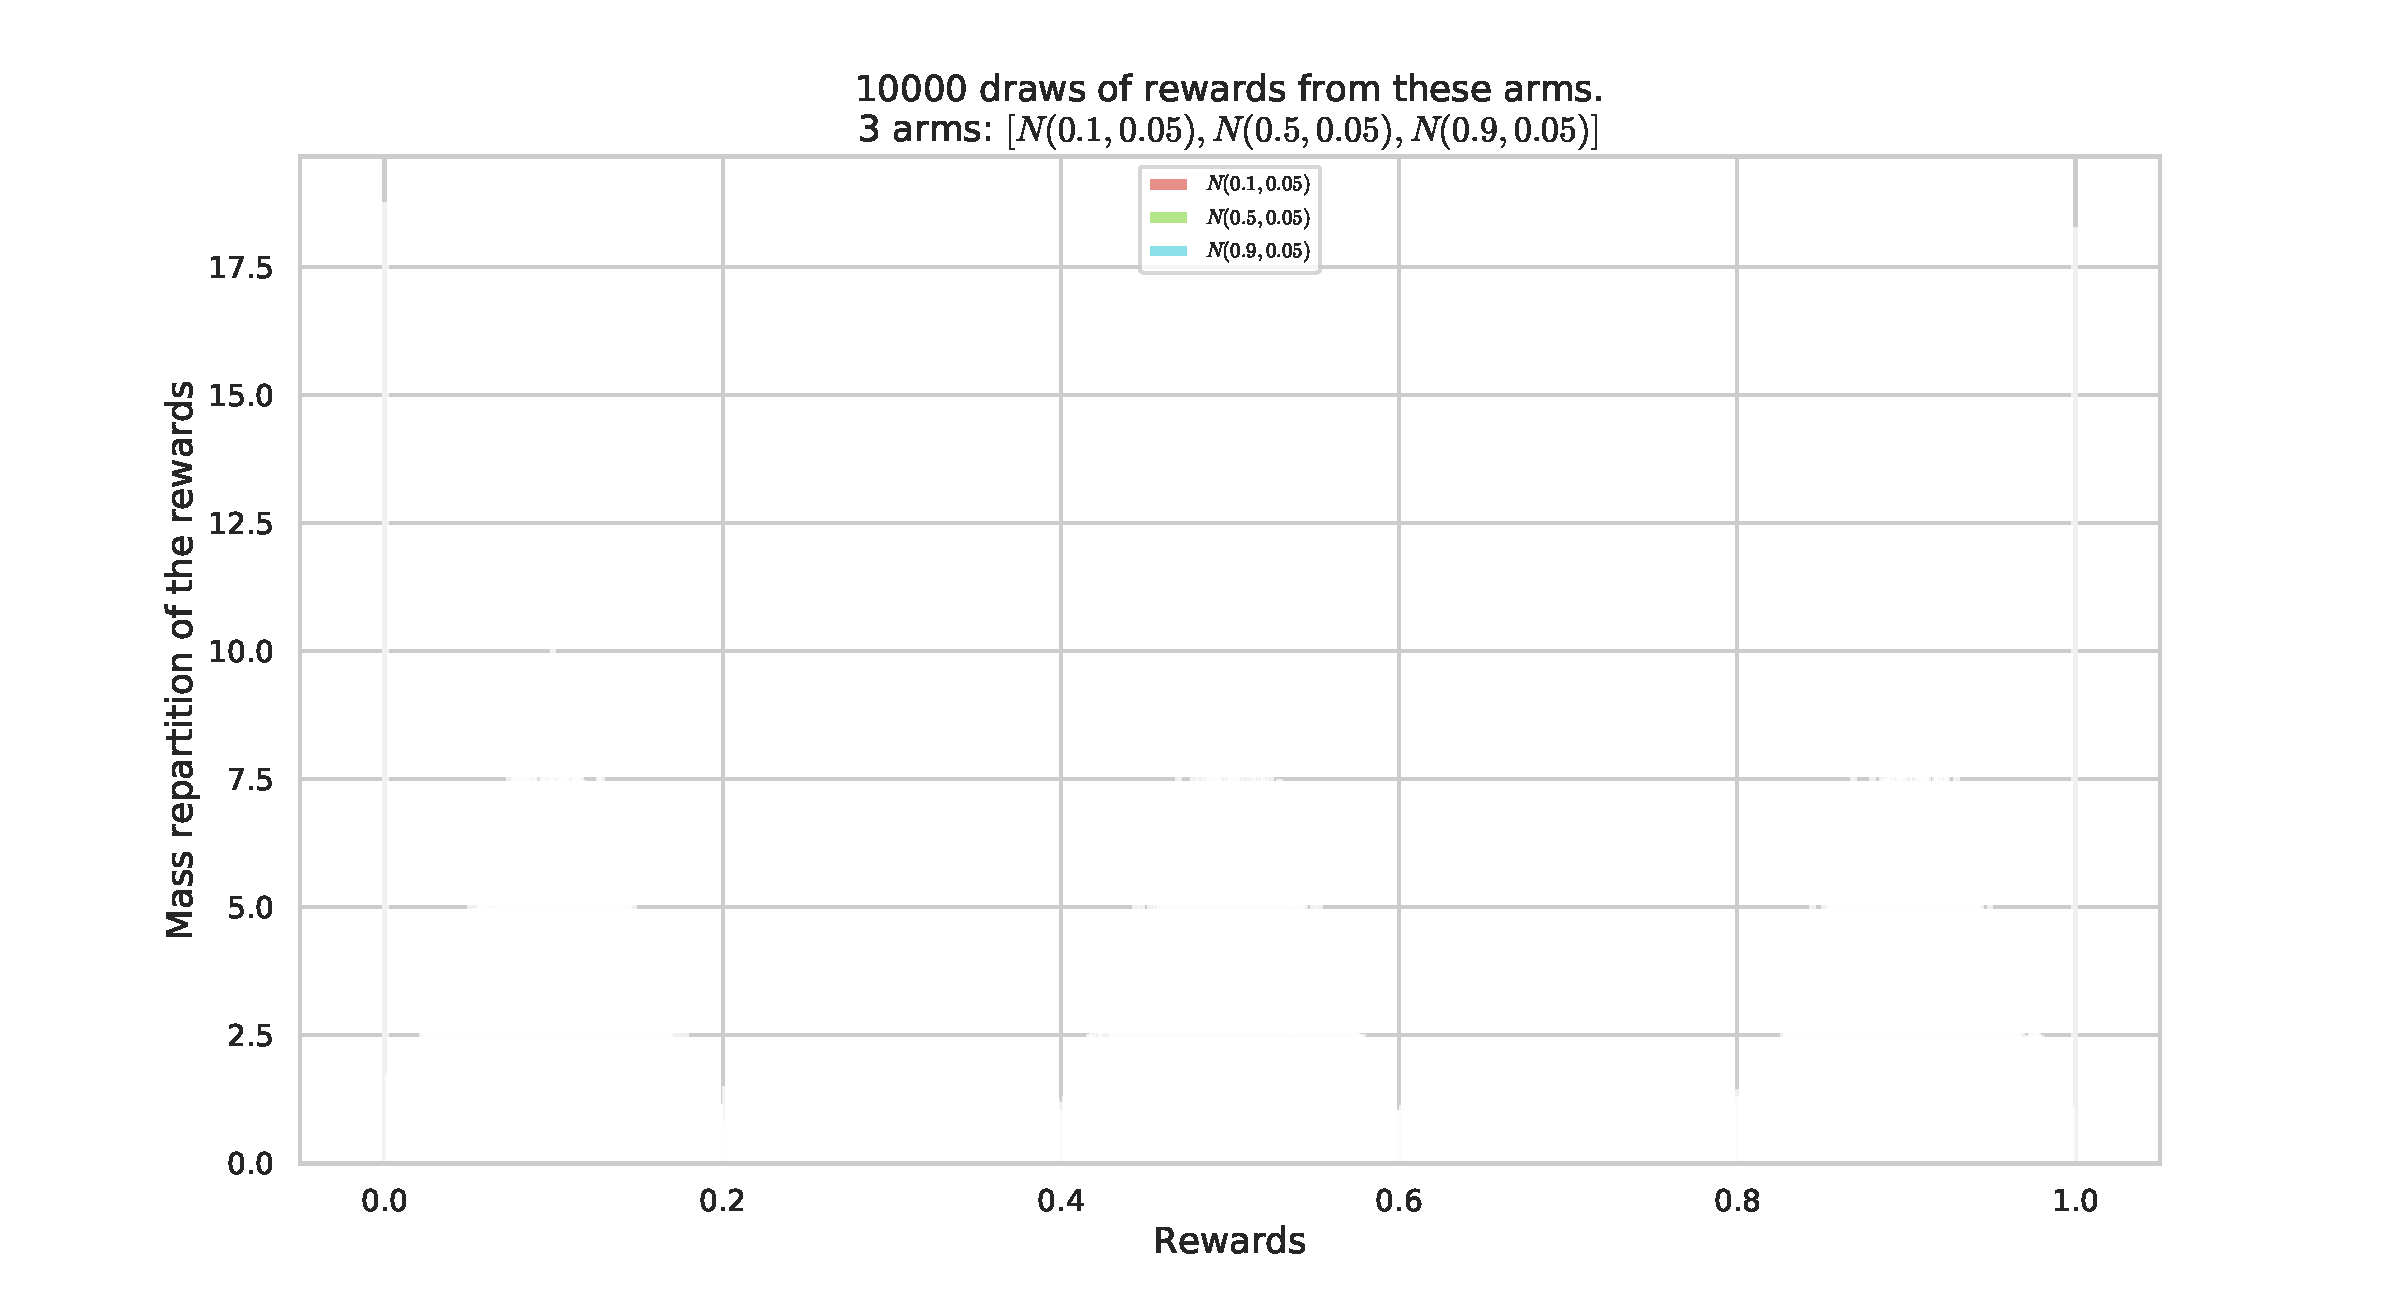
\includegraphics[width=0.75\linewidth]{exampleOfRewards.pdf}
	\caption{Histogram of $10000$ \iid{} rewards obtained from three arms with a Gaussian distribution truncated to $[0,1]$, of respective means $0.1$, $0.5$ and $0.9$.}
	\label{fig:3:exampleOfRewards}
\end{figure}

For more details, an interested reader can refer to the following Jupyter notebook \cite{jupyter}:
\begin{small}
    \href{https://smpybandits.github.io/notebooks/Easily_creating_MAB_problems.html}{\texttt{SMPyBandits.GitHub.io/notebooks/Easily\_creating\_MAB\_problems.html}}
\end{small}

We have not yet tried to add support for higher dimensional distributions of rewards, \eg, linear bandit, but it would be an interesting extension of SMPyBandits.
%
However, note that our library does support finite-state real-valued Markov MAB models, where arms do not correspond to distributions but to Markov chains, in the two variants of \emph{rested} or \emph{restless} Markov chains, as introduced by \cite{Anantharam87b}.

\subsection{MAB algorithms}

SMPyBandits is a complete open-source implementation of single-player (classical) bandit algorithms,
containing over 65 algorithms (in the module \texttt{\href{https://SMPyBandits.GitHub.io/docs/Policies.html}{Policies}}).
It uses a well-designed hierarchical structure and class inheritance scheme (as detailed on the various UML diagrams showed on the \texttt{\href{https://SMPyBandits.GitHub.io/uml_diagrams/README.html}{uml\_diagrams}} folder) to minimize redundancy in the codebase.
For instance, most existing algorithms are index-based, and new ones can be written easily by inheriting from the \texttt{IndexPolicy} class (\texttt{\href{https://SMPyBandits.GitHub.io/docs/Policies.IndexPolicy.html}{Policies.IndexPolicy}}).
An index-based algorithm computes an index $I_k(t)\in\mathbb{R}$ for each arm $k$ at time $t$ and simply play $A(t) = \arg\max_k I_k(t)$.
For instance the code specific to the UCB algorithm \cite{LaiRobbins85,Auer02} is as short as this (and fully documented):

% https://tex.stackexchange.com/a/12430/
\begin{small}
% \begin{listing}[h!]
    \inputminted[linenos=true,numbersep=5pt,frame=lines,framesep=2mm]{python3}{2-Chapters/3-Chapter/src/example_of_a_IndexPolicy_UCB.py}
    % \caption{Small snippet of code defining the UCB algorithm, as a simple example of an Index Policy}
    \captionof{listing}{Small snippet of code defining the UCB algorithm, as a simple example of an Index Policy \label{lst:3:smallIndexPolicy}.}
    % \label{lst:3:smallIndexPolicy}
% \end{listing}
\end{small}


\subsection{Summary of the features}

With this numerical framework, simulations can run on a single CPU or a multi-core machine using joblib \cite{joblib} (see Appendix~\ref{sub:3:parallelSimulations}),
and summary plots are automatically saved as high-quality PNG, PDF and EPS, using matplotlib \cite{matplotlib} and seaborn \cite{seaborn}.
Raw data from each simulation is also saved in a HDF5 file using h5py \cite{h5py}, an efficient and compressed binary format, to allow easy post-mortem exploration of simulation results.
Making new simulations is very easy, one only needs to write a configuration script (\texttt{configuration.py}), without needing a complete knowledge of the internal code architecture.


\subsection{Documentation}

A complete documentation, for each algorithm and the entire codebase, is available online at
% even including the constants in the different configuration files:
\texttt{\href{https://SMPyBandits.GitHub.io}{SMPyBandits.GitHub.io}}.
It uses the Sphinx software \cite{sphinx}, and the content is directly written in the Python files as docstring, to allow users to have access to the documentation from within their IDE or the Python console.
The most interesting component of the library is the many algorithms being implemented: for each of them, the documentation gives at least a reference to a research paper (\eg, \cite{Kaufmann12BUCB} for \texttt{BayesUCB}), as well as a bird-eye view of its behavior.
For most algorithms, in particular for index policies, the internal variables of the implementation are carefully linked with the notations of each paper, and formulas explaining the way the algorithm selects its arm are usually given.
Whenever it is appropriate, the documentation also includes warning or information about the empirical performance of costly algorithms.
The documentation also contains extensive examples of any intermediate numerical functions, that are also used as tests (using \texttt{doctest.testmod} from the standard library).
For example, Figures~\ref{fig:3:twoScreenshotsOfTheDocumentation} and \ref{fig:3:twoMoreScreenshotsOfTheDocumentation} below show four screenshots from the documentation.
We show the main page, the list of algorithms in the \texttt{Policies} module, an example of the documentation of one algorithm (for the \klUCB-Switch algorithm from \cite{Garivier18}), and a page detailing the API and organization of the library as well as instructions to follow if someone wants to implement a new model or a new algorithm.

\begin{figure}[h!]  % [htbp]
    \centering
	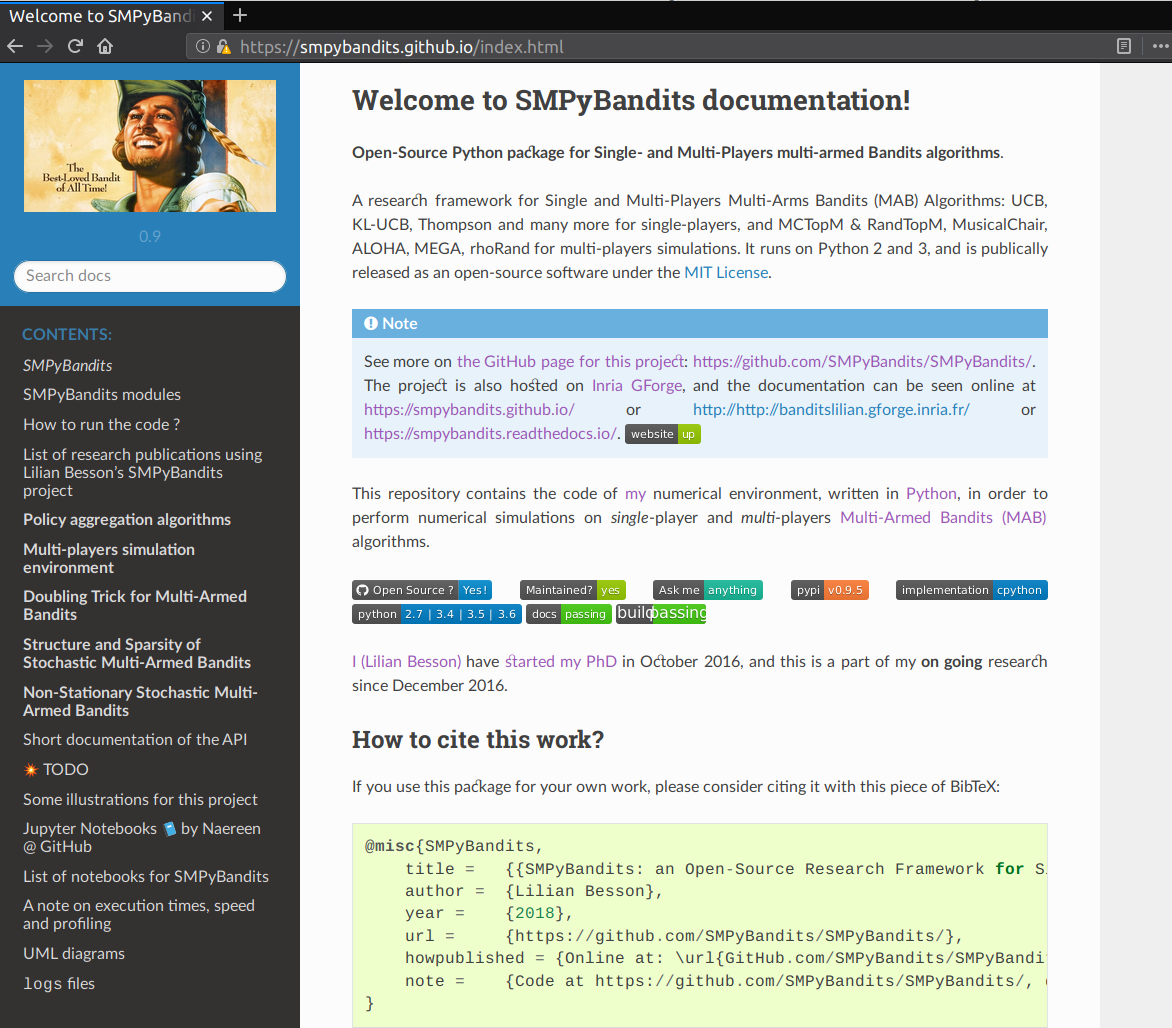
\includegraphics[width=0.49\linewidth]{overview_documentation_1.png}
    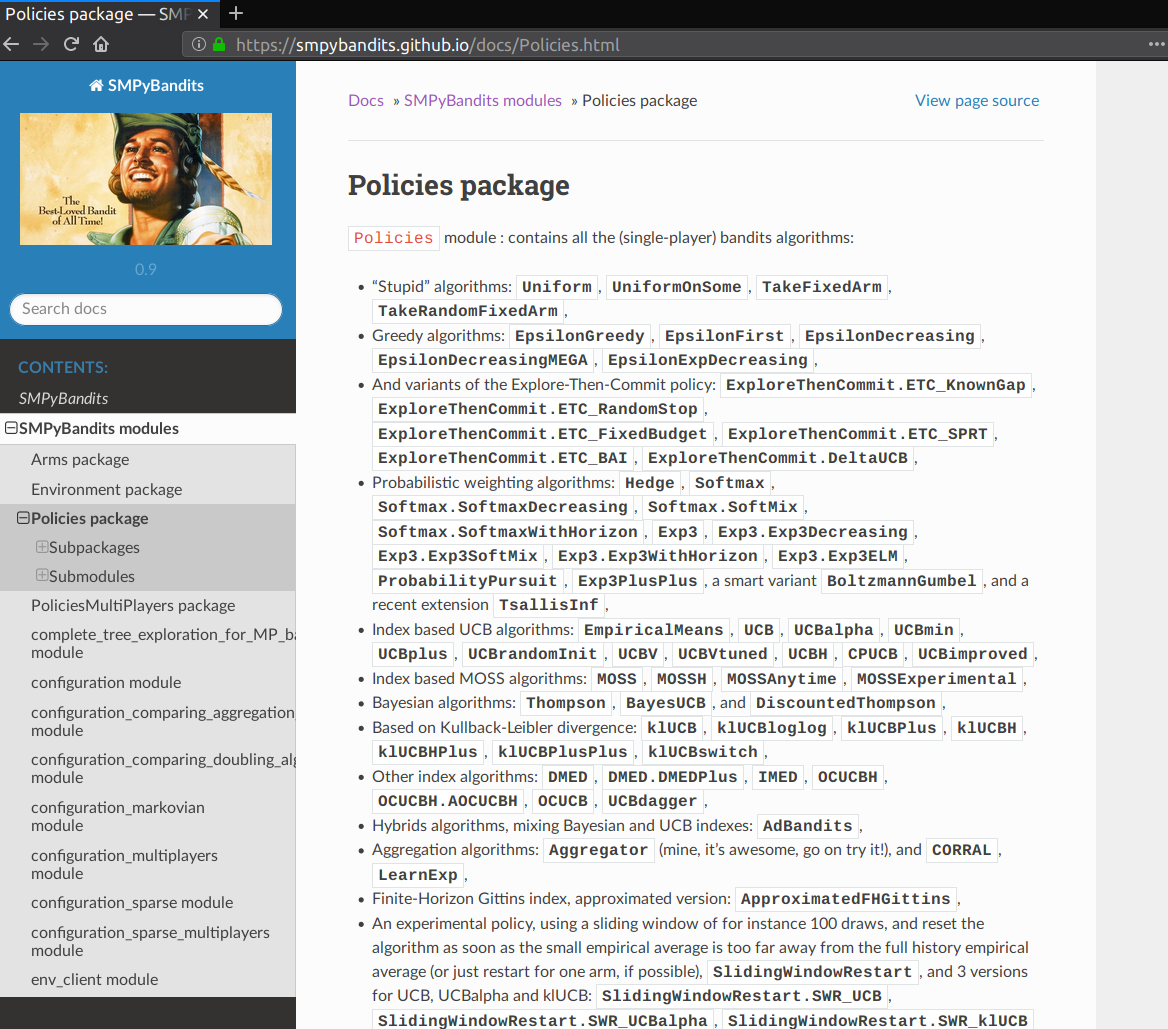
\includegraphics[width=0.49\linewidth]{overview_documentation_2.png}
	\caption{Screenshots from two pages of the documentation.}
	\label{fig:3:twoScreenshotsOfTheDocumentation}
\end{figure}

\begin{figure}[h!]  % [htbp]
    \centering
	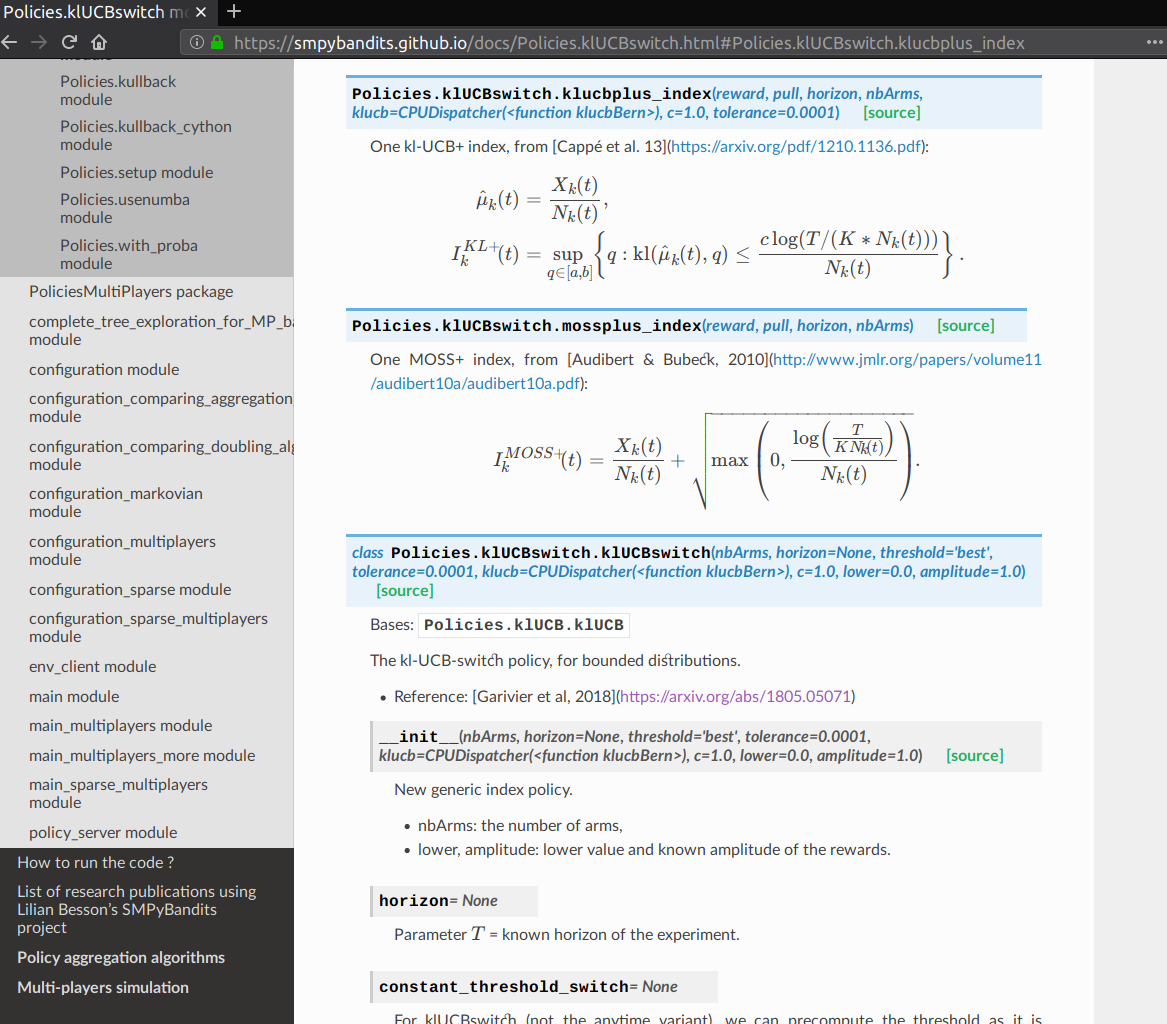
\includegraphics[width=0.49\linewidth]{overview_documentation_3.png}
	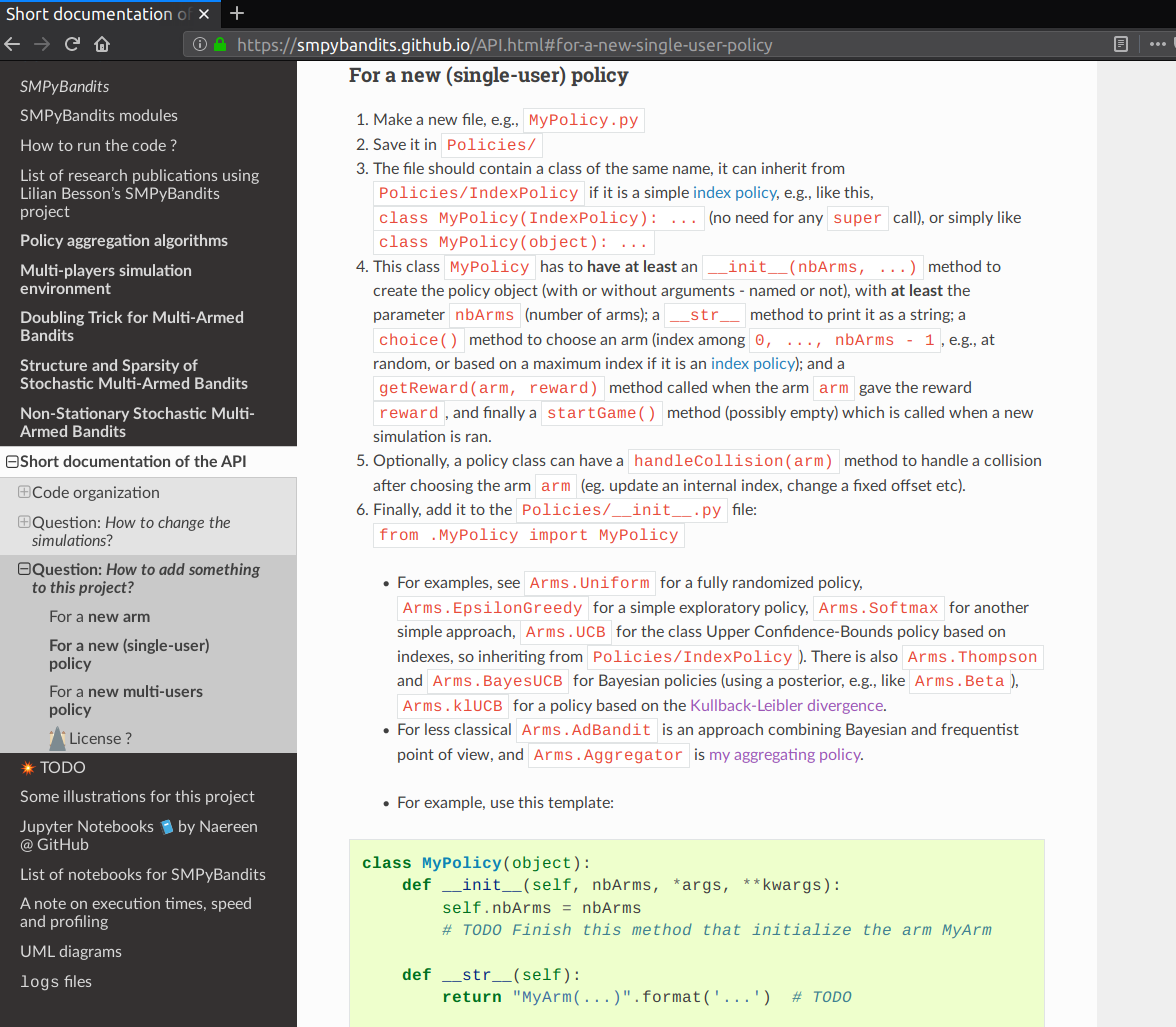
\includegraphics[width=0.49\linewidth]{overview_documentation_4.png}
	\caption{Screenshots from two other pages of the documentation.}
	\label{fig:3:twoMoreScreenshotsOfTheDocumentation}
\end{figure}


\subsection{How to run experiments?}

We show how to install SMPyBandits, and an example of how to run a simple experiment.
This bash snippet\footnote{~See this page \texttt{\href{https://SMPyBandits.GitHub.io/How_to_run_the_code.html}{SMPyBandits.GitHub.io/How\_to\_run\_the\_code.html}} for more details.} shows how to clone the code\footnote{~SMPyBandits is also available on Pypi, see \texttt{\href{https://pypi.org/project/SMPyBandits/}{pypi.org/project/SMPyBandits}}. You can install it directly with \texttt{sudo pip install SMPyBandits}, or from a \texttt{virtualenv} \cite{virtualenv}.},
and install the requirements for Python 3 (once):

% https://tex.stackexchange.com/a/12430/
\begin{small}
    \begin{listing}[h!]
        \begin{minted}[linenos=true,numbersep=5pt,frame=lines,framesep=2mm]{bash}
# 1. get the code in the folder you want
$ git clone https://GitHub.com/SMPyBandits/SMPyBandits.git
$ cd SMPyBandits.git
# 2. install the requirements
$ pip install -r requirements.txt
        \end{minted}
        \caption{Small snippet of Bash code to download and install dependencies of SMPyBandits.}
        % \captionof{listing}{Small snippet of Bash code to download and install dependencies of SMPyBandits \label{lst:3:howToInstallLibrary}.}
        \label{lst:3:howToInstallLibrary}
    \end{listing}
\end{small}

Launching simulations is easy, for instance this snippet shows how to start $N=1000$ repetitions of a simple non-Bayesian Bernoulli-distributed problem, for $K=9$ arms, an horizon of $T=10000$ and on $4$ CPUs.
It takes about $20$ minutes, on a standard $4$-cores $64$ bits GNU/Linux laptop.
Using environment variables (\texttt{N=1000} etc) in the command line is not required, but it is convenient:

% https://tex.stackexchange.com/a/12430/
\begin{small}
\begin{listing}[h!]
    \begin{minted}[linenos=true,numbersep=5pt,frame=lines,framesep=2mm]{bash}
# 3. run a single-player simulation
$ BAYES=False ARM_TYPE=Bernoulli N=1000 T=10000 K=9 N_JOBS=4 \
  MEANS=[0.1,0.2,0.3,0.4,0.5,0.6,0.7,0.8,0.9] \
  python3 main.py configuration.py
    \end{minted}
    \caption{Small snippet of Bash code to run a simple experiment with SMPyBandits.}
    % \captionof{listing}{Small snippet of Bash code to run a simple experiment with SMPyBandits \label{lst:3:howToRunBasicLibrary}.}
    \label{lst:3:howToRunBasicLibrary}
\end{listing}
\end{small}


\subsection{Example of a simulation and illustration}

A small script \texttt{configuration.py}
% (\texttt{\href{https://SMPyBandits.GitHub.io/docs/configuration.html}{SMPyBandits.GitHub.io/docs/configuration.html}})
is used to import the arm classes (\texttt{\href{https://SMPyBandits.GitHub.io/docs/Arms.html}{Arms}} module), the policy classes (\texttt{\href{https://SMPyBandits.GitHub.io/docs/Policies.html}{Policies}} module) and define the problems and the experiments.
Choosing the algorithms to include is done by changing
the \texttt{configuration["policies"]} list in the \texttt{configuration.py} file.
For instance, one can compare the standard anytime \klUCB{} algorithm (class \texttt{\href{https://SMPyBandits.GitHub.io/docs/Policies.klUCB.html}{klUCB}} in \texttt{Policies} module) against the non-anytime variant $\klUCB^{++}$ algorithm (\texttt{\href{https://SMPyBandits.GitHub.io/docs/Policies.klUCBPlusPlus.html}{klUCBPlusPlus}}), and also \UCB{} with $\alpha=1$ (\texttt{\href{https://SMPyBandits.GitHub.io/docs/Policies.UCBalpha.html}{UCB}}) and Thompson sampling (\texttt{\href{https://SMPyBandits.GitHub.io/docs/Policies.Thompson.html}{Thompson}}) with a Beta posterior (\texttt{\href{https://SMPyBandits.GitHub.io/docs/Policies.Posterior.Beta.html}{Posterior.Beta}})).

% https://tex.stackexchange.com/a/12430/
\begin{small}
\begin{listing}[h!]
    \begin{minted}[linenos=true,numbersep=5pt,frame=lines,framesep=2mm]{python3}
configuration["policies"] = [
  {"archtype": klUCB, "params": {"klucb": klucbBern}},
  {"archtype": klUCBPlusPlus,
   "params": {"horizon": T, "klucb": klucbBern}},
  {"archtype": UCBalpha, "params": {"alpha": 1}},
  {"archtype": Thompson, "params": {"posterior": Beta}}
]
    \end{minted}
    \caption{Small snippet of Python code to configure the list of algorithms tested on a problem.}
    % \captionof{listing}{Small snippet of Python code to configure the list of algorithms tested on a problem. \label{lst:3:howToConfigureAlgorithms}.}
    \label{lst:3:howToConfigureAlgorithms}
\end{listing}
\end{small}

\begin{figure}[h!]  % [htbp]
	\centering
	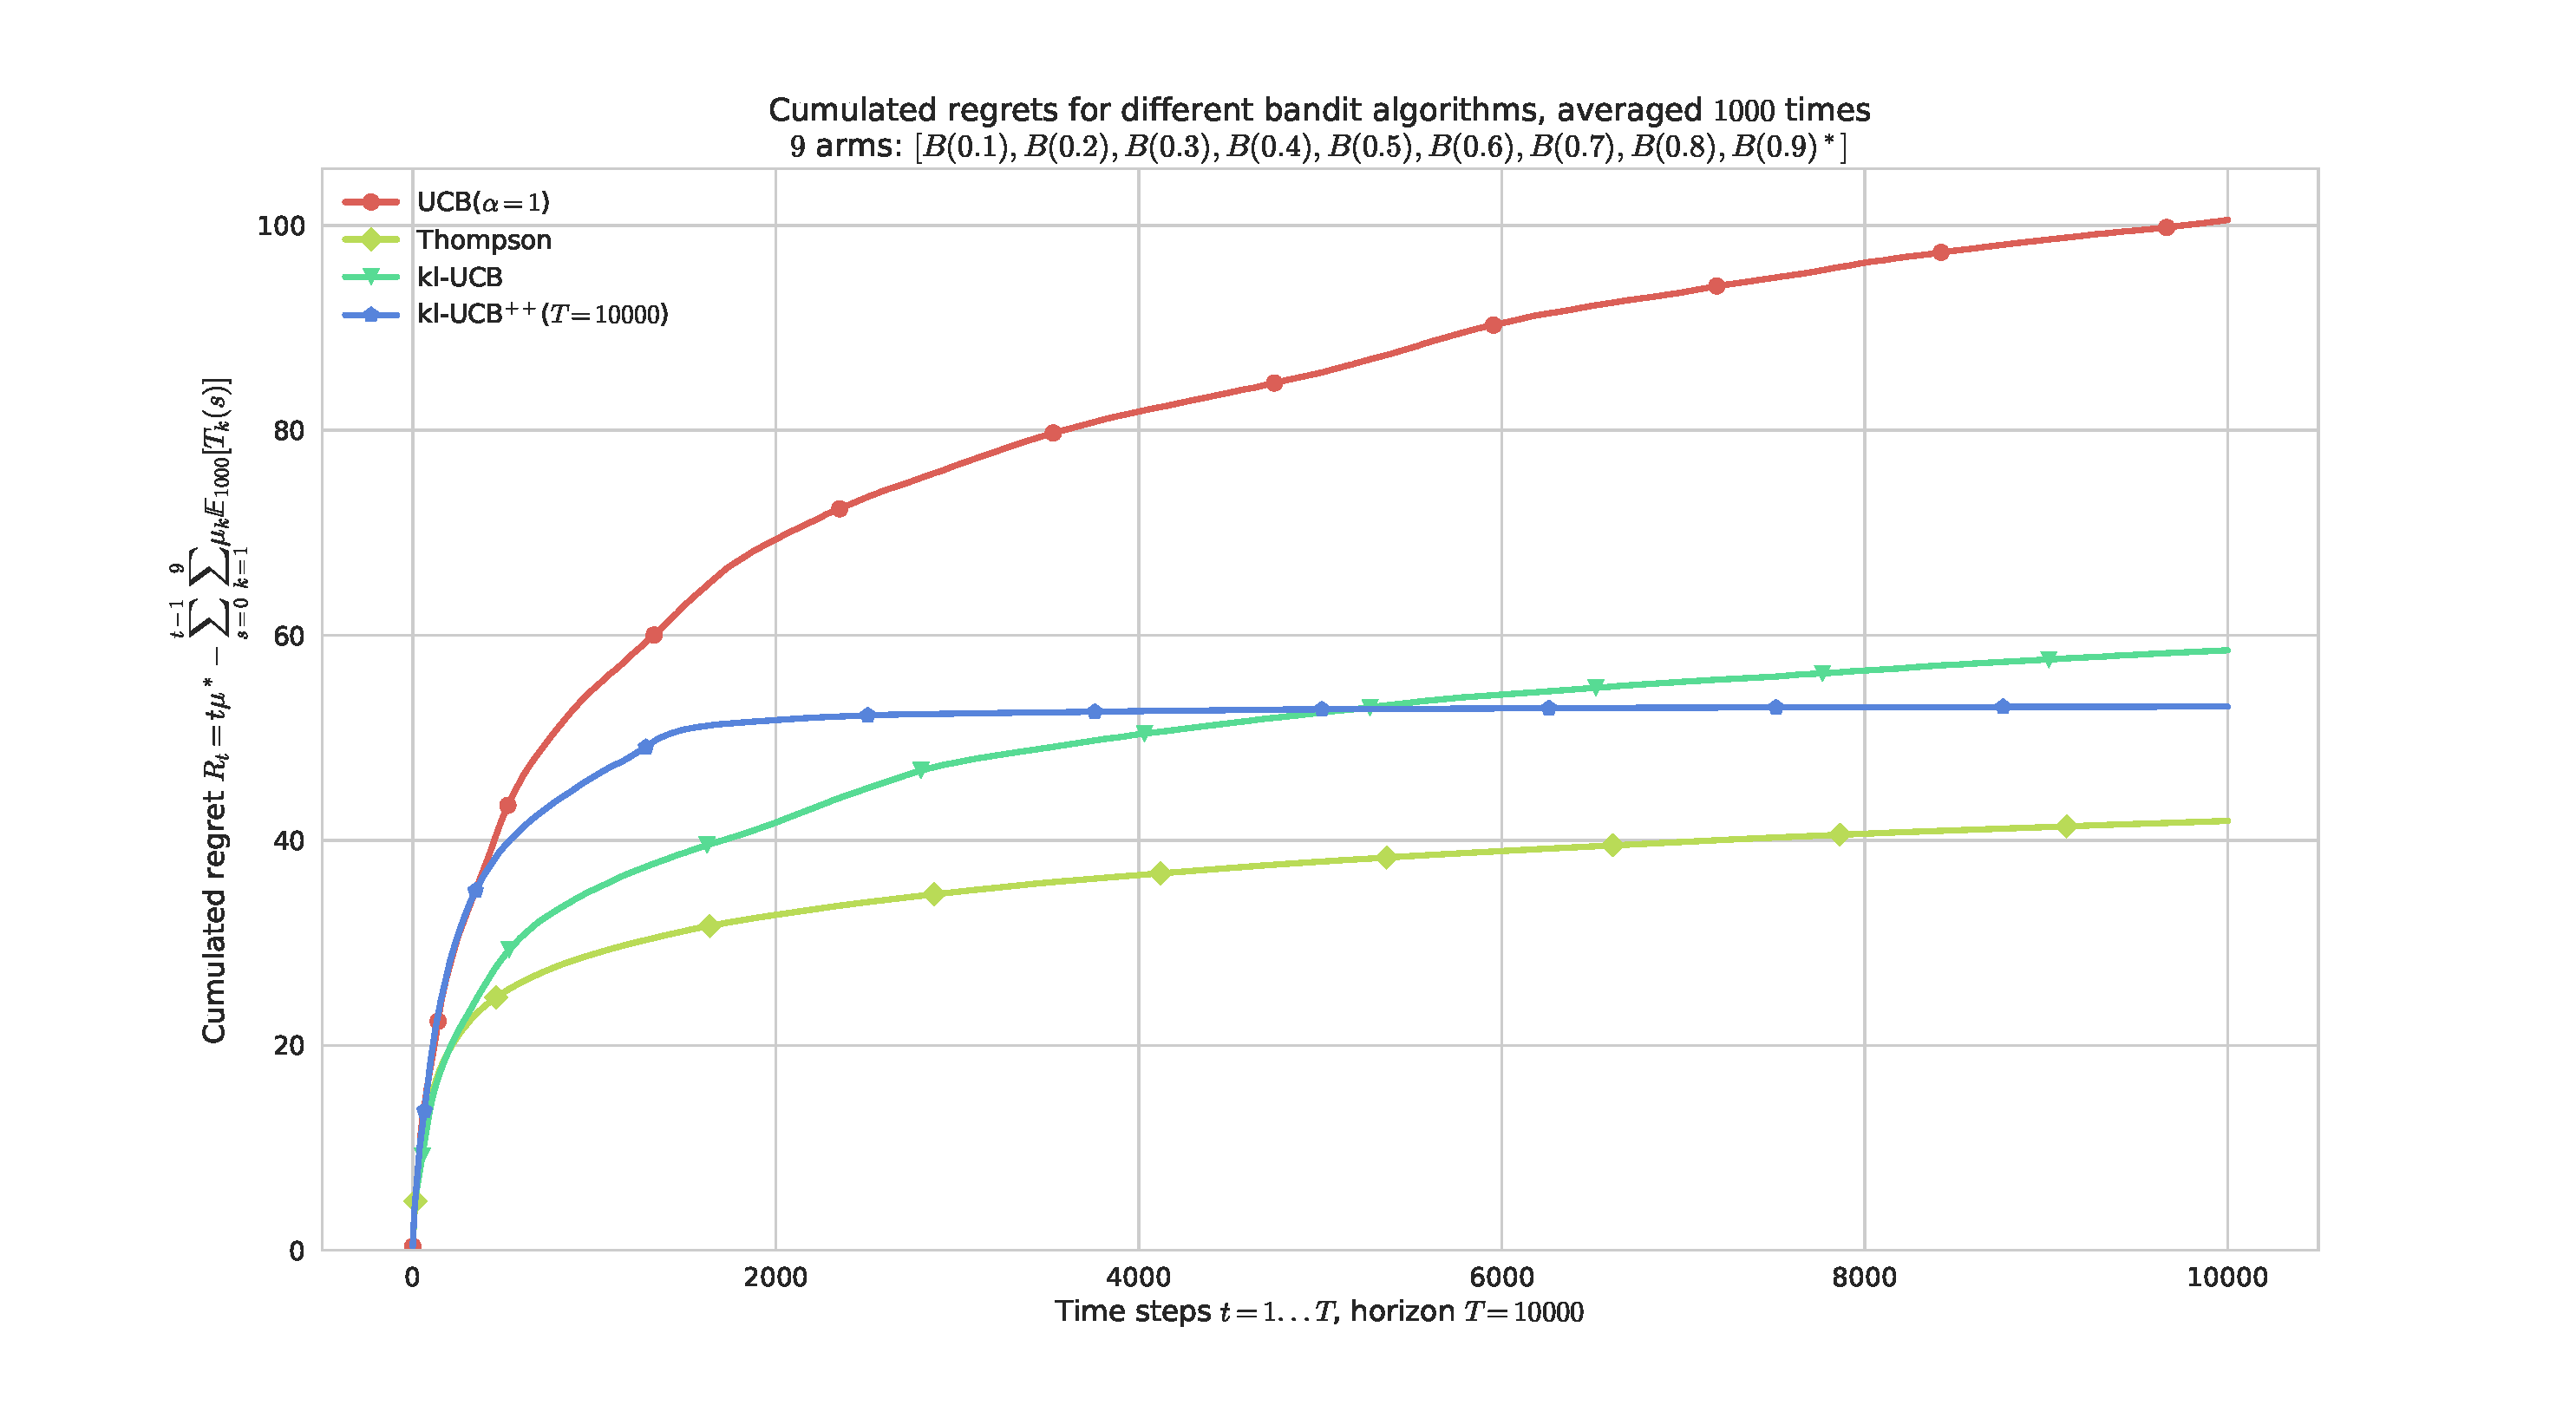
\includegraphics[width=1.05\linewidth]{3.pdf}
	\caption[Example of a single-player simulation showing the average regret of $4$ algorithms]{
		Example of a single-player simulation showing the average regret of four algorithms. They all perform very well: each algorithm is known to be order-optimal (\ie, its regret is proved to match the lower-bound up-to a constant), and each but UCB is known to be asymptotically optimal (\ie, with the constant matching the lower-bound).
	}
	\label{fig:3:firstPlot}
\end{figure}

Running the simulation as shown above will save figures in a sub-folder, as well as save data (pulls, rewards, regret and other data) in a HDF5 file\footnote{~For example, this simulation produced this HDF5 file\\\texttt{\href{https://github.com/SMPyBandits/SMPyBandits/blob/master/plots/paper/example.hdf5}{GitHub.com/SMPyBandits/SMPyBandits/blob/master/plots/paper/example.hdf5}}}
\cite{h5py}.
% \texttt{\href{http://docs.h5py.org/en/stable/high/file.html}{docs.h5py.org/en/stable/high/file.html}}).
Figure~\ref{fig:3:firstPlot} above shows the average regret for these $4$ algorithms.
% The regret is the difference between the cumulated rewards of the best fixed-armed strategy (which is the oracle strategy for stationary bandits), and the cumulated rewards of the considered algorithms.
The Figure~\ref{fig:3:firstPlot_hist} below shows the histogram of regret obtained at the end of the experiment (\ie, $R_T$) for the same example.

\begin{figure}[h!]  % [htbp]
	\centering
	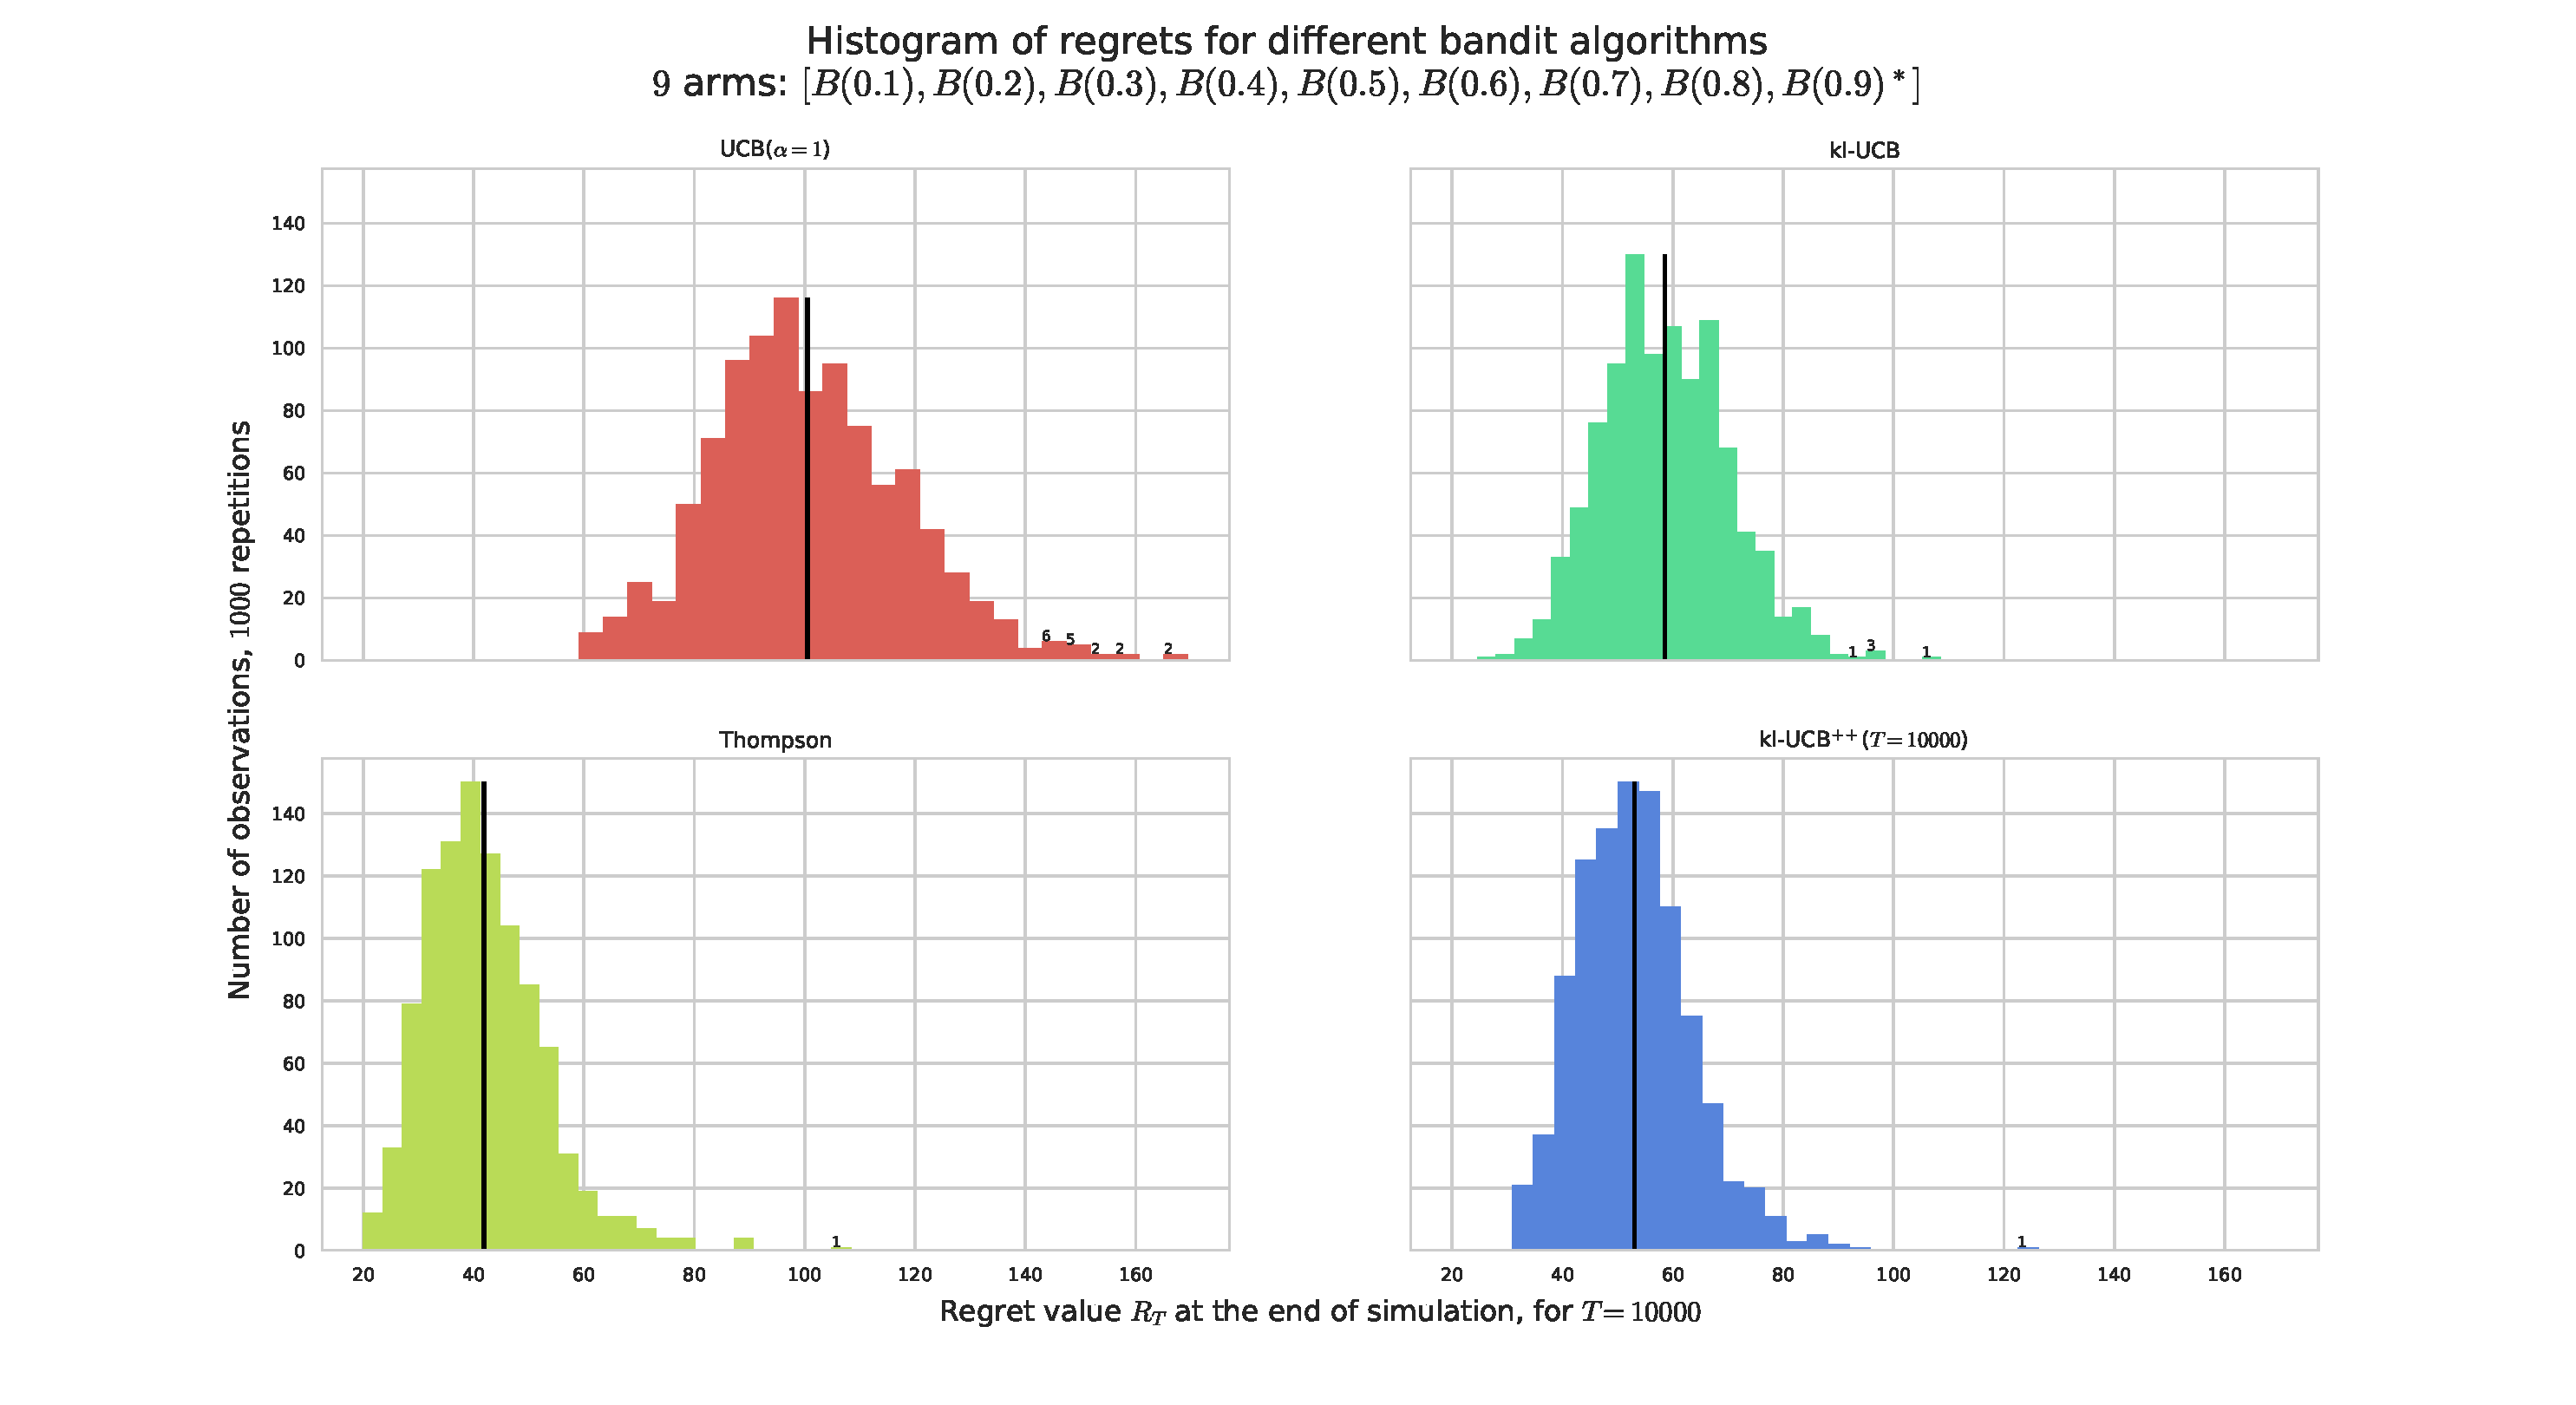
\includegraphics[width=1.05\linewidth]{3_hist.pdf}
	\caption{Histogram of regret for the same experiment as of Figure~\ref{fig:3:firstPlot}. For instance, Thomson sampling is very efficient in average (in yellow), and UCB shows a larger variance (in red).}
	\label{fig:3:firstPlot_hist}
\end{figure}


\subsection{Dependencies}
\label{sub:3:dependencies}

This library is written in Python \cite{python}, for versions 2.7+ or 3.4+, using \texttt{matplotlib} \cite{matplotlib} for 2D plotting, \texttt{numpy} \cite{numpy} for data storing, random number generations and operations on arrays, \texttt{scipy} \cite{scipy} for statistical and special functions, and \texttt{seaborn} \cite{seaborn} for pretty plotting and colorblind-aware colormaps.

Optional dependencies include \texttt{joblib} \cite{joblib} for parallel simulations, \texttt{numba} \cite{numba} for automatic speed-up on small functions using a Just-in-Time compiler, \texttt{sphinx} \cite{sphinx} for generating the documentation, \texttt{virtualenv} \cite{virtualenv} for launching simulations in isolated environments, and \texttt{jupyter} \cite{jupyter} used with \texttt{ipython} \cite{ipython} to experiment with the code.

All the quoted libraries are free and open-source and can be installed in one command using the \texttt{pip} (\texttt{\href{https://pip.pypa.io/}{pip.PyPa.io}}) or \texttt{conda} (\texttt{\href{http://conda.anaconda.org/}{conda.anaconda.org}}) package manager.
%
When SMPyBandits is installed using \texttt{pip install SMPyBandits}, the dependencies are of course automatically installed if not already present.


\subsection{Continuous integration with Read the Docs and Travis CI}

% \TODOL{I need to quickly explain that SMPyBandits is using Read the Docs since $2017$ and Travis Ci since $2018$ to: }

Since $2017$ and $2018$, SMPyBandits is using two online continuous integration (CI) service, to automatically build and host the documentation, and to automatically test the library on some numerical simulations.
%
These CI services are free for open-source works, and are both triggered whenever a modification of the codebase is sent to the hosting platform (\ie, GitHub).

\paragraph{Read the Docs.}
Since $2017$, we have been using the free web service provided by Read the Docs (\href{https://readthedocs.org/}{\texttt{ReadTheDocs.org}}).
Read the Docs allows to automatically build the documentation after every commit. This allows to regularly check that the library is well formatted and can be imported correctly, as well as keeping the online documentation up-to-date.
Moreover, they offer to host the documentation online, at \href{https://smpybandits.rtfd.io/}{\texttt{SMPyBandits.ReadTheDocs.io}}.
For more details, see \href{https://readthedocs.org/projects/smpybandits/}{\texttt{ReadTheDocs.org/projects/SMPyBandits}}.
%
Since its first use, the service did about 180 builds, and about $10\%$ of them were useful to detect newly introduced issues or bugs in the code.
The build is configured using the \texttt{.readthedocs.yml} file in SMPyBandits main folder, and it builds the documentation in about two minutes.
I have also been building the documentation manually on a weekly basis, to also host it on \href{https://smpybandits.github.io/}{\texttt{SMPyBandits.GitHub.io}} thanks to GitHub pages.
In the last two years, the documentation saw about 8500 unique visits, while the GitHub project have been visited about 3500 unique visits.


\paragraph{Travis CI.}
Since $2018$, we have been using the free web service provided by Travis CI (\href{https://travis-ci.org/}{\texttt{Travis-CI.org}}).
Travis CI allows to automatically run short numerical simulations after every commit.
This allows to check that each modification on any part of the codebase does not break anything, as well as giving an up-to-date example of log files that shows online the results of different examples of experiments. The tests covers all the main models and almost all the algorithms implemented in SMPyBandits, and it has been proven very useful to quickly find and fix new bugs.
For more details, see \href{https://travis-ci.org/SMPyBandits/SMPyBandits}{\texttt{Travis-CI.org/SMPyBandits/SMPyBandits}}.
%
Since its first use, the service did about 160 builds, and about $30\%$ of them were useful to detect newly introduced issues or bugs in the code.
The build is configured using the \texttt{.travis.yml} file in SMPyBandits main folder, and it runs numerical experiments with a short horizon (\eg, $T=100$ or $T=1000$) and a small number of repetitions (\ie, $N=4$), but covering all the different models implemented by SMPyBandits (and even including some that are not covered in this chapter, like the Markov model, or the sparse multi-player model).
Builds typically run for $15$ minutes, and Travis CI have been proven to be very useful in our development process.



\subsection{List of research works using SMPyBandits}

SMPyBandits has been used for the following research articles since $2017$, and it is used for the previous and the next chapters of this thesis (except in Chapter~\ref{chapter:4}).

-- In \cite{Besson2018WCNC} and in Chapter~\ref{chapter:2} above, we used SMPyBandits to illustrate and compare different aggregation algorithms\footnote{~See the page \texttt{\href{https://SMPyBandits.GitHub.io/Aggregation.html}{SMPyBandits.GitHub.io/Aggregation.html}} on the documentation, which gives detailed instructions to reproduce the results presented in this research paper, details about the models and the notations, and bibliographic references.}. We designed a variant of the Exp4 algorithm for online aggregation of experts \cite{Bubeck12}, called \texttt{\href{https://SMPyBandits.GitHub.io/docs/Policies.Aggregator.html}{Aggregator}}.
% Aggregating experts is a well-studied idea in sequential learning and in machine learning in general. We showed that it can be used in practice to select on the run the best bandit algorithm for a certain problem from a fixed pool of experts. This idea and algorithm can have interesting impact for Opportunistic Spectrum Access applications \cite{Jouini09} that use multi-armed bandits algorithms for sequential learning and network efficiency optimization.

-- In \cite{Besson2018ALT} and in Chapter~\ref{chapter:5} below, we used SMPyBandits for all the simulations for multi-player bandit algorithms\footnote{~Similarly, see the page \texttt{\href{https://SMPyBandits.GitHub.io/MultiPlayers.html}{SMPyBandits.GitHub.io/MultiPlayers.html}} on the documentation.}. We designed the two \texttt{\href{https://SMPyBandits.GitHub.io/docs/PoliciesMultiPlayers.RandTopM.html}{RandTopM}} and \texttt{\href{https://SMPyBandits.GitHub.io/docs/PoliciesMultiPlayers.MCTopM.html}{MCTopM}} algorithms and proved than they obtain logarithmic regret in the usual setting, and outperform significantly the previous state-of-the-art solutions (\ie, \texttt{\href{https://SMPyBandits.GitHub.io/docs/PoliciesMultiPlayers.rhoRand.html}{rhoRand}}, \texttt{\href{https://SMPyBandits.GitHub.io/docs/Policies.MEGA.html}{MEGA}} and \texttt{\href{https://SMPyBandits.GitHub.io/docs/Policies.MusicalChair.html}{MusicalChair}}).

-- In \cite{Besson2018DoublingTricks} (quickly presented in Appendix~\ref{app:2:DoublingTricks}), we used SMPyBandits to illustrate and compare different "doubling trick" schemes\footnote{~Similarly, see the page \texttt{\href{https://SMPyBandits.GitHub.io/DoublingTrick.html}{SMPyBandits.GitHub.io/DoublingTrick.html}} on the documentation.}.
In sequential learning, an algorithm is said to be ``anytime'' if it does not need to know the horizon $T$ of the experiments. A well-known trick for transforming any ``non-anytime'' algorithm to an ``anytime'' variant is the ``Doubling Trick'': start with an horizon $T_0\in\mathbb{N}^*$, and when $t > T_i$, use $T_{i+1} = 2 T_i$. We studied two generic sequences of growing horizons (geometric and exponential), and we proved two theorems that generalized previous results. A geometric sequence suffices to keep minimax regret bounds (in $R_T = \mathcal{O}(\sqrt{T})$), with a constant multiplicative loss $\ell \leq 4$, but cannot be used to keep a logarithmic regret bound (in $R_T = \mathcal{O}(\log(T))$). And an exponential sequence can be used to keep logarithmic bounds, with a constant multiplicative loss also $\ell \leq 4$ in the usual setting. It is still an open question to know if a well-tuned exponential sequence can keep minimax bounds, or "weak" minimax bounds (in $R_T = \mathcal{O}(\sqrt{T \log(T)})$).

-- In \cite{Besson2019GLRT} and \cite{Besson2019Gretsi}, and in Chapter~\ref{chapter:6} below, we used SMPyBandits for piece-wise stationary MAB models (only for the single-player case). We illustrate and compare different algorithms designed for this family of non-stationary problems\footnote{~Similarly, see the page \texttt{\href{https://SMPyBandits.GitHub.io/NonStationary.html}{SMPyBandits.GitHub.io/NonStationary.html}} on the documentation.}.
We designed the \texttt{\href{https://SMPyBandits.GitHub.io/docs/Policies.GLR_UCB.html}{GLRklUCB}} policy, and implemented most of the policies from state-of-the-art research on passively or active adaptive policies, both adversarial- or stochastic-based, designed to tackle the piece-wise stationary MAB problems.
We also implemented a large benchmark of different problems.


% ----------------------------------------------------------------------------
\section{Experimental comparisons of state-of-the-art algorithms}
\label{sec:3:reviewSPAlgorithms}

% \TODOL{Write text for this Section, write configuration.py file, run short-term experiment, include them, if happy about it, run longer ang larger experiments}

In this section, we use the SMPyBandits library to compare experimentally various state-of-the-art single-player algorithms on some multi-armed bandit problems.
First, we detail the list of different algorithms that we compare, and the different problems on which they are all tested.
We give the results of the numerical experiments, in terms of mean regret at the end of the experiment of different horizons $T$.
Additional results in terms of real measurements of time and memory are given and discussed in the next Section~\ref{sec:3:timeAndMemoryCosts}.

Finally, we give some observations on the results, and the main take-away message of this section is the following: in all the rest of this thesis, we focus on two algorithms depending if simplicity or efficiency is favored:
\begin{itemize}
    \item
    \UCB{} is used in the more applied Chapter~\ref{chapter:4}, when simplicity is favored,
    \item
    \klUCB{} is used, in the two more theoretical Chapters~\ref{chapter:5} and \ref{chapter:6}, when efficiency is favored.
\end{itemize}


\subsection{Experimental setup: algorithms and problems}

% \paragraph{List of algorithms}

We consider the nine following algorithms, and seven more are described in Appendix~\ref{sub:3:additionalExperiments}.
For each of them, we give a bibliographic reference, that corresponds to a recent article studying it and not the first one which introduced it.
We give the chosen tuning of the parameters, for parametric algorithms.
Algorithms that are ``not anytime'' use the exact value of the horizon $T$, and when increasing values of $T$ are studied for the same problem, they use the correct successive values. \\
%
\indent
For reproducibility, we also give in ``\texttt{typewriter font}'' the name of the corresponding class in the \texttt{Policies} module in SMPyBandits
(\eg, $\UCB_1$ is \texttt{Policies.UCBalpha}).

\begin{itemize}
    \item Algorithm 1 is
    an $\varepsilon$-greedy algorithm, as described in \cite{Bubeck12}, using $\varepsilon_t = \varepsilon_0 / t$, and $\varepsilon_0 = 0.1$ (chosen arbitrarily) (\texttt{EpsilonDecreasing}).
    It has a very small cost in terms of time and memory, but it usually achieves linear regret.

    \item Algorithm 2 is
    an Explore-then-Commit algorithm from \cite{GarivierETC2016}, that knows the horizon, and a lower-bound on the gap between arms (chosen arbitrarily as $\delta=0.01$, valid for all problems) (\texttt{ETC\_KnownGap}).
    Similarly to $\varepsilon$-greedy, it has a very small footprint in terms of time and memory, but only obtain large (linear) regret.

    \item Algorithm 3 is
    $\mathrm{Exp}3^{++}$ from \cite{Seldin17}, using $\alpha=3$ and $\beta=256$ as advised (\texttt{Exp3PlusPlus}).
    It is a recent variant of the $\mathrm{Exp3}$ algorithm, using an adaptive tuning of its parameter. It is anytime, and was proven to obtain good ``best of both world'' performances, meaning that it achieves $\cO(K\log(T)/\Delta^2)$ regret for problem-dependent bounds, and $\cO(\sqrt{KT})$ for problem-independent bounds.

    \item Algorithm 4 is
    $\UCB_1$ from \cite{Auer02}, using $\alpha=1$ (\texttt{UCBalpha}).
    It achieves order-optimal problem-dependent bounds with a $\cO(K\log(T)/\Delta^2)$ regret.

    \item Algorithm 5 is
    \klUCB{} from \cite{KLUCBJournal}, using the Bernoulli KL divergence and the corresponding \klUCB{} indexes, implemented as \texttt{kullback.klucbBern} (\texttt{klUCB}).
    It achieves asymptotical optimal problem-dependent bounds with a $\cO(\log(T))$ regret with the scaling factor matching Lai and Robbins' lower-bound \cite{LaiRobbins85}.
    It is computationally more costly that \UCB, as at each time step $t$ and for each arm $k$, a convex optimization problem must be solved approximately, in order to compute the $K$ indexes.
    In practice, a few steps of a simple Newton method are enough to obtain a good numerical precision, and empirically we found that even in the worst cases \klUCB{} is no more than an order of magnitude slower than \UCB.
    % of more than 10 digits
    \TODOL{Si on en pas parlé avant, ou après dans une annexe, je peux dire un mot ici à propos de l'implémentation en Cython ou en C des fonctions kl et indices kl-UCB !}

    \item Algorithm 6 is
    Thompson sampling from \cite{Kaufmann12Thompson}, using a Beta prior and posterior, initially uniform (\ie, $\mathrm{Beta}(1,1)$) (\texttt{Thompson}).
    It was also proved to achieve asymptotical optimal problem-dependent bounds \cite{Kaufmann12Thompson,AgrawalGoyal11}.
    It is efficient in terms of storage, and even if $K$ random samples must be sampled from the arms posteriors at each time step $t$, Thompson sampling is not much slower than \UCB, if the random number generator used for the simulations is efficient (it is the case for SMPyBandits, as we use \texttt{numpy.random} module which relies on C or Cython code, highly optimized).

    \item Algorithm 7 is
    Bayes-UCB from \cite{Kaufmann12BUCB}, using a Beta prior and posterior, initially uniform (\ie, $\mathrm{Beta}(1,1)$) (\texttt{BayesUCB}).
    It was also proved to achieve asymptotical optimal problem-dependent bounds \cite{Kaufmann12BUCB}.
    It is comparable to Thompson sampling in terms of memory complexity, but slower in terms of time complexity as computing a $1-1/t$ quantile is more costly than sampling from a distribution.
    But in particular for Bernoulli distributed arms and for Beta posteriors and priors, Bayes-UCB is only about twice as slow as Thompson sampling.

    \item Algorithm 8 is
    AdBandits from \cite{Truzzi13}, using $\alpha=1$ (\texttt{AdBandits}).
    It follows the same assumptions as Thompson sampling and Bayes-UCB, and uses a Beta posterior on each arm. It uses a random mixture between the two algorithms, and with a certain probability it uses the Thompson decision rule (\ie, choose the arm maximizing one draw of random samples from the posteriors), otherwise it uses the Bayes-UCB decision rule (\ie, choose the arm maximizing the $1-1/t$ quantile).
    It was proposed in this article \cite{Truzzi13} and illustrated on empirical simulations, but no theoretical analysis was given, and it did not gain popularity since then.
    In practice, it is usually (slighly) more efficient than both Thompson sampling and Bayes-UCB in terms of regret, it is comparable in terms of computation times, but costs more memory.

    \item Algorithm 9 is
    BESA (Best Empirical Sampled Average) from \cite{Baransi2014}, and it consists in trying to fix a simple observation.
    For instance in \UCB, if arm $1$ has $100$ samples and arm $2$ has $50$ samples, it should make more sense to only use $50$ samples of arm $1$ to compute and compare any statistics for each arms (\eg, mean).
    The BESA algorithm for $K=2$ arms is then very simple: at each time step, if arms $1$ and $2$ have $n_1$ and $n_2$ samples, and if $n_1>n_2$ (for instance), first it sub-samples $n_2$ observations from $n_1$, then it computes the mean of these observations, and play the arm maximizing this mean (now that there is the same number of observations for both arms, it makes more sense to compare these quantities).
    It was analyzed partially for the two-armed case, and the authors illustrated that it can be very efficient empirically.
    Analyzing it in the generic case was found to be difficult, and is still an open problem.
    We implemented it using a binary tournament implement in a naive but efficient way (not using recursive functions, \ie, using the \texttt{BESA} class with \texttt{''non\_recursive''=True}).
    By using such binary tournament, the extension $K>2$ arms is costly in terms of both time and memory, as illustrated below, and suffer from an exponential blow-up when $K$ increases.
\end{itemize}

We focussed here on the most well known algorithms, and two others that are efficient but less known (AdBandits and BESA),
but to illustrate that SMPyBandits implements many other solutions to the MAB problem proposed in very recent works, we explain in Appendix~\ref{sub:3:additionalExperiments} seven other algorithms.
They are more recent (some from $2016$, $3$ from $2018$ and $2$ from early $2019$) and are usually more complex, or are based on a different point-of-view.
The numerical results presented below include these extra algorithms, to justify empirically that despite their respective qualities, and despite being very efficient, it is reasonable to focus on \UCB{} and \klUCB{} algorithms in the rest of this thesis, as they stay comparable with the state-of-the-art algorithms but are simpler to implement (\eg, when comparing \UCB{} to \texttt{ApproximatedFHGittins} or $\mathrm{MOSS}$-$\mathrm{Anytime}$) to manipulate theoretically (\eg, when comparing \klUCB{} to PHE or RCB)


\paragraph{Two different problems}

We consider two different problems, that are described here for a generic value of $K \geq 2$ the number of arms.
For simplicity, we focus on Bernoulli distributed arms, even if similar results were observed for other distributions, in particular for truncated or untruncated Gaussian distributions.

\begin{itemize}
    \item \textbf{Problem 1} considers $K$ arms of equally spaced means, in $[0,1]$.
    It uses a minimum mean of $0.05$ and a maximum mean of $0.95$.
    For instance, for $K=2$, $\bm{\mu}=[0.05, 0.95]$ and for $K=5$, $\bm{\mu} = [0.05, 0.275, 0.5, 0.725, 0.95]$.

    \item \textbf{Problem 2} takes another approach. Instead of simulating $1000$ times the same problem, it generates a new random problem for each independent run.
    It considers a randomly generated vector of means, each being sampled uniformly at random in $[0,1]$, with a minimum gap of $\Delta^{\min}$, $\bm{\mu} \sim \cE(\Delta^{\min},\mu_{\min},\mu_{\max})$, as well as minimum and maximum values of $\mu_{\min}$ and $\mu_{\max}$.
    This space $\cE_{\Delta^{\min}}$ is defined as $\{ \bm{\mu} \in [\mu_{\min}, \mu_{\max}]^K : \min_{k\neq k'} |\mu_k - \mu_{k'}| \geq \Delta^{\min} \}$.
    We use $\mu_{\min} = \Delta^{\min}$ and $\mu_{\max} = 1 - \Delta^{\min}$,
    and the value used for $\Delta^{\min}$ is $0.1$ for $K \leq 3$ (for ``easy'' problems), and $\frac{1}{3 K}$ for $K \geq 5$ (for ``harder'' problems).
    % 0.1 if NB_ARMS <= 5 else 1. / (3 * NB_ARMS)
\end{itemize}


\paragraph{Other parameters of the experiments}

% FIXME update if needed?
We consider increasing values for the horizon, and we focus on $7$ exponentially-spaced values: $T=1000$, $T=2500$, $T=5000$, $T=10000$, $T=20000$, $T=25000$ and $T=50000$.
We consider as well an increasing number of arms, and we focus again on $7$ values: $K=2$, $K=4$, $K=8$, $K=12$, $K=16$, $K=20$ and $K=32$.
For all experiments, we run $N=100$ independent simulations.
We show in the snippet of code~\ref{lst:3:BashCodeToLaunchLargeExperiments} in the Appendix below more details about how to run these experiments.

\TODOL{Dans les figures où je montre une seule valeur de $T$ ou de $K$, et $R_T$, $\cT_T$ ou $\cM_T$ en fonction de $K$ ou de $T$, il faudrait avoir plus de valeurs à montrer, et pas une progression exponentielle... J'ai relancé avec :
    - $T=10000$ et $K = 6, 10, 14, 18, 22, 24, 26, 28, 32$ pour couvrir $2 \dots 32$ avec un pas de $2$,
    - $K=32$ et $T = 15000, 30000, 35000, 40000, 45000$ pour couvrir $5000 \dots 50000$ avec un pas de $5000$,
}


\subsection{Experiments results}

We give in the figures below the results of the experiments.
% For the two different problems and different values of $T$ and $K$, we give the mean $\pm 1$ standard-variation of the empirical regret $R_T$ obtained by the different algorithms at the end of the experiments.
% Tables~\ref{table:3:meanRegret_problem1} is for the fixed-gap \textbf{problem 1}
% and \ref{table:3:meanRegret_problem2} is for the randomly generated \textbf{problem 2}.
% Each column corresponds to one value of $T$, and each line corresponds to one algorithm.
% For each cell, we report successive values that correspond to the successive values of the number of arms $K$.


% \TODOL{FIXME launch these experiments, for a very short number of repetitions N=4, and if I'm happy about the results and if they are easily copied-and-pasted here, then launch with N=100 or N=1000 depending on the running time of the whole simulations}

% DEBUG=True; NOPLOTS=False; SAVEALL=False; for N in 4 100 1000; do for BAYES in False True; do for T in 1000 5000 10000 50000; do for K in 2 5 10 20 50; do debut=$(date); DEBUG=$DEBUG NOPLOTS=$NOPLOTS SAVEALL=$SAVEALL N=$N N_JOBS=-1 T=$T K=$K BAYES=$BAYES make --noFreeSMS single && cp logs/main_py3_log.txt logs/main_py3_log__N${N}_BAYES${BAYES}_T{T}_K{K}.txt && FreeSMS.py "Expérience commencée ${debut} terminée, avec N=${N}, BAYES=${BAYES}, T=${T}, K=${K}." ; done; done; done; done time.

% \begin{table}[!t]
% \begin{footnotesize}  % WARNING
%     \centering
%     \begin{tabular}{c|*{5}{m{2cm}}} % WARNING size ?
%     \textbf{Algorithms} $\;$ \textbackslash $\;$ $\mathbf{T=}$
%         & $T_1 = 1000$ & $T_2 = 5000$ & $T_3 = 10000$ & $T_4 = 50000$ \\
%         \hline
%         $\varepsilon$-greedy &
%             $R^{1}_{T_1,K_1} = 0 \pm 0$
%                 $R^{1}_{T_1,K_2} = 0 \pm 0$
%                 $R^{1}_{T_1,K_3} = 0 \pm 0$
%                 $R^{1}_{T_1,K_4} = 0 \pm 0$
%                 $R^{1}_{T_1,K_5} = 0 \pm 0$ &
%             $R^{1}_{T_2,K_1} = 0 \pm 0$
%                 $R^{1}_{T_2,K_2} = 0 \pm 0$
%                 $R^{1}_{T_2,K_3} = 0 \pm 0$
%                 $R^{1}_{T_2,K_4} = 0 \pm 0$
%                 $R^{1}_{T_2,K_5} = 0 \pm 0$ &
%             $R^{1}_{T_3,K_1} = 0 \pm 0$
%                 $R^{1}_{T_3,K_2} = 0 \pm 0$
%                 $R^{1}_{T_3,K_3} = 0 \pm 0$
%                 $R^{1}_{T_3,K_4} = 0 \pm 0$
%                 $R^{1}_{T_3,K_5} = 0 \pm 0$ &
%             $R^{1}_{T_4,K_1} = 0 \pm 0$
%                 $R^{1}_{T_4,K_2} = 0 \pm 0$
%                 $R^{1}_{T_4,K_3} = 0 \pm 0$
%                 $R^{1}_{T_4,K_4} = 0 \pm 0$
%                 $R^{1}_{T_4,K_5} = 0 \pm 0$ \\
%         \hline
%         Explore-then-Commit &
%             $R^{2}_{T_1,K_1} = 0 \pm 0$
%                 $R^{2}_{T_1,K_2} = 0 \pm 0$
%                 $R^{2}_{T_1,K_3} = 0 \pm 0$
%                 $R^{2}_{T_1,K_4} = 0 \pm 0$
%                 $R^{2}_{T_1,K_5} = 0 \pm 0$ &
%             $R^{2}_{T_2,K_1} = 0 \pm 0$
%                 $R^{2}_{T_2,K_2} = 0 \pm 0$
%                 $R^{2}_{T_2,K_3} = 0 \pm 0$
%                 $R^{2}_{T_2,K_4} = 0 \pm 0$
%                 $R^{2}_{T_2,K_5} = 0 \pm 0$ &
%             $R^{2}_{T_3,K_1} = 0 \pm 0$
%                 $R^{2}_{T_3,K_2} = 0 \pm 0$
%                 $R^{2}_{T_3,K_3} = 0 \pm 0$
%                 $R^{2}_{T_3,K_4} = 0 \pm 0$
%                 $R^{2}_{T_3,K_5} = 0 \pm 0$ &
%             $R^{2}_{T_4,K_1} = 0 \pm 0$
%                 $R^{2}_{T_4,K_2} = 0 \pm 0$
%                 $R^{2}_{T_4,K_3} = 0 \pm 0$
%                 $R^{2}_{T_4,K_4} = 0 \pm 0$
%                 $R^{2}_{T_4,K_5} = 0 \pm 0$ \\
%         \hline
%         $\mathrm{Exp}3^{++}$ &
%             $R^3_{T_1,K_1} = 0 \pm 0$
%                 $R^3_{T_1,K_2} = 0 \pm 0$
%                 $R^3_{T_1,K_3} = 0 \pm 0$
%                 $R^3_{T_1,K_4} = 0 \pm 0$
%                 $R^3_{T_1,K_5} = 0 \pm 0$ &
%             $R^3_{T_2,K_1} = 0 \pm 0$
%                 $R^3_{T_2,K_2} = 0 \pm 0$
%                 $R^3_{T_2,K_3} = 0 \pm 0$
%                 $R^3_{T_2,K_4} = 0 \pm 0$
%                 $R^3_{T_2,K_5} = 0 \pm 0$ &
%             $R^3_{T_3,K_1} = 0 \pm 0$
%                 $R^3_{T_3,K_2} = 0 \pm 0$
%                 $R^3_{T_3,K_3} = 0 \pm 0$
%                 $R^3_{T_3,K_4} = 0 \pm 0$
%                 $R^3_{T_3,K_5} = 0 \pm 0$ &
%             $R^3_{T_4,K_1} = 0 \pm 0$
%                 $R^3_{T_4,K_2} = 0 \pm 0$
%                 $R^3_{T_4,K_3} = 0 \pm 0$
%                 $R^3_{T_4,K_4} = 0 \pm 0$
%                 $R^3_{T_4,K_5} = 0 \pm 0$ \\
%         \hline
%         $\UCB_1$ &
%             $R^{4}_{T_1,K_1} = 0 \pm 0$
%                 $R^{4}_{T_1,K_2} = 0 \pm 0$
%                 $R^{4}_{T_1,K_3} = 0 \pm 0$
%                 $R^{4}_{T_1,K_4} = 0 \pm 0$
%                 $R^{4}_{T_1,K_5} = 0 \pm 0$ &
%             $R^{4}_{T_2,K_1} = 0 \pm 0$
%                 $R^{4}_{T_2,K_2} = 0 \pm 0$
%                 $R^{4}_{T_2,K_3} = 0 \pm 0$
%                 $R^{4}_{T_2,K_4} = 0 \pm 0$
%                 $R^{4}_{T_2,K_5} = 0 \pm 0$ &
%             $R^{4}_{T_3,K_1} = 0 \pm 0$
%                 $R^{4}_{T_3,K_2} = 0 \pm 0$
%                 $R^{4}_{T_3,K_3} = 0 \pm 0$
%                 $R^{4}_{T_3,K_4} = 0 \pm 0$
%                 $R^{4}_{T_3,K_5} = 0 \pm 0$ &
%             $R^{4}_{T_4,K_1} = 0 \pm 0$
%                 $R^{4}_{T_4,K_2} = 0 \pm 0$
%                 $R^{4}_{T_4,K_3} = 0 \pm 0$
%                 $R^{4}_{T_4,K_4} = 0 \pm 0$
%                 $R^{4}_{T_4,K_5} = 0 \pm 0$ \\
%         \hline
%         \klUCB{} &
%             $R^{5}_{T_1,K_1} = 0 \pm 0$
%                 $R^{5}_{T_1,K_2} = 0 \pm 0$
%                 $R^{5}_{T_1,K_3} = 0 \pm 0$
%                 $R^{5}_{T_1,K_4} = 0 \pm 0$
%                 $R^{5}_{T_1,K_5} = 0 \pm 0$ &
%             $R^{5}_{T_2,K_1} = 0 \pm 0$
%                 $R^{5}_{T_2,K_2} = 0 \pm 0$
%                 $R^{5}_{T_2,K_3} = 0 \pm 0$
%                 $R^{5}_{T_2,K_4} = 0 \pm 0$
%                 $R^{5}_{T_2,K_5} = 0 \pm 0$ &
%             $R^{5}_{T_3,K_1} = 0 \pm 0$
%                 $R^{5}_{T_3,K_2} = 0 \pm 0$
%                 $R^{5}_{T_3,K_3} = 0 \pm 0$
%                 $R^{5}_{T_3,K_4} = 0 \pm 0$
%                 $R^{5}_{T_3,K_5} = 0 \pm 0$ &
%             $R^{5}_{T_4,K_1} = 0 \pm 0$
%                 $R^{5}_{T_4,K_2} = 0 \pm 0$
%                 $R^{5}_{T_4,K_3} = 0 \pm 0$
%                 $R^{5}_{T_4,K_4} = 0 \pm 0$
%                 $R^{5}_{T_4,K_5} = 0 \pm 0$ \\
%         \hline
%         Thompson sampling &
%             $R^{6}_{T_1,K_1} = 0 \pm 0$
%                 $R^{6}_{T_1,K_2} = 0 \pm 0$
%                 $R^{6}_{T_1,K_3} = 0 \pm 0$
%                 $R^{6}_{T_1,K_4} = 0 \pm 0$
%                 $R^{6}_{T_1,K_5} = 0 \pm 0$ &
%             $R^{6}_{T_2,K_1} = 0 \pm 0$
%                 $R^{6}_{T_2,K_2} = 0 \pm 0$
%                 $R^{6}_{T_2,K_3} = 0 \pm 0$
%                 $R^{6}_{T_2,K_4} = 0 \pm 0$
%                 $R^{6}_{T_2,K_5} = 0 \pm 0$ &
%             $R^{6}_{T_3,K_1} = 0 \pm 0$
%                 $R^{6}_{T_3,K_2} = 0 \pm 0$
%                 $R^{6}_{T_3,K_3} = 0 \pm 0$
%                 $R^{6}_{T_3,K_4} = 0 \pm 0$
%                 $R^{6}_{T_3,K_5} = 0 \pm 0$ &
%             $R^{6}_{T_4,K_1} = 0 \pm 0$
%                 $R^{6}_{T_4,K_2} = 0 \pm 0$
%                 $R^{6}_{T_4,K_3} = 0 \pm 0$
%                 $R^{6}_{T_4,K_4} = 0 \pm 0$
%                 $R^{6}_{T_4,K_5} = 0 \pm 0$ \\
%         \hline
%         Thompson sampling &
%             $R^{7}_{T_1,K_1} = 0 \pm 0$
%                 $R^{7}_{T_1,K_2} = 0 \pm 0$
%                 $R^{7}_{T_1,K_3} = 0 \pm 0$
%                 $R^{7}_{T_1,K_4} = 0 \pm 0$
%                 $R^{7}_{T_1,K_5} = 0 \pm 0$ &
%             $R^{7}_{T_2,K_1} = 0 \pm 0$
%                 $R^{7}_{T_2,K_2} = 0 \pm 0$
%                 $R^{7}_{T_2,K_3} = 0 \pm 0$
%                 $R^{7}_{T_2,K_4} = 0 \pm 0$
%                 $R^{7}_{T_2,K_5} = 0 \pm 0$ &
%             $R^{7}_{T_3,K_1} = 0 \pm 0$
%                 $R^{7}_{T_3,K_2} = 0 \pm 0$
%                 $R^{7}_{T_3,K_3} = 0 \pm 0$
%                 $R^{7}_{T_3,K_4} = 0 \pm 0$
%                 $R^{7}_{T_3,K_5} = 0 \pm 0$ &
%             $R^{7}_{T_4,K_1} = 0 \pm 0$
%                 $R^{7}_{T_4,K_2} = 0 \pm 0$
%                 $R^{7}_{T_4,K_3} = 0 \pm 0$
%                 $R^{7}_{T_4,K_4} = 0 \pm 0$
%                 $R^{7}_{T_4,K_5} = 0 \pm 0$ \\
%         \hline
%         AdBandits &
%             $R^{8}_{T_1,K_1} = 0 \pm 0$
%                 $R^{8}_{T_1,K_2} = 0 \pm 0$
%                 $R^{8}_{T_1,K_3} = 0 \pm 0$
%                 $R^{8}_{T_1,K_4} = 0 \pm 0$
%                 $R^{8}_{T_1,K_5} = 0 \pm 0$ &
%             $R^{8}_{T_2,K_1} = 0 \pm 0$
%                 $R^{8}_{T_2,K_2} = 0 \pm 0$
%                 $R^{8}_{T_2,K_3} = 0 \pm 0$
%                 $R^{8}_{T_2,K_4} = 0 \pm 0$
%                 $R^{8}_{T_2,K_5} = 0 \pm 0$ &
%             $R^{8}_{T_3,K_1} = 0 \pm 0$
%                 $R^{8}_{T_3,K_2} = 0 \pm 0$
%                 $R^{8}_{T_3,K_3} = 0 \pm 0$
%                 $R^{8}_{T_3,K_4} = 0 \pm 0$
%                 $R^{8}_{T_3,K_5} = 0 \pm 0$ &
%             $R^{8}_{T_4,K_1} = 0 \pm 0$
%                 $R^{8}_{T_4,K_2} = 0 \pm 0$
%                 $R^{8}_{T_4,K_3} = 0 \pm 0$
%                 $R^{8}_{T_4,K_4} = 0 \pm 0$
%                 $R^{8}_{T_4,K_5} = 0 \pm 0$ \\
%         \hline
%         BESA &
%             $R^{9}_{T_1,K_1} = 0 \pm 0$
%                 $R^{9}_{T_1,K_2} = 0 \pm 0$
%                 $R^{9}_{T_1,K_3} = 0 \pm 0$
%                 $R^{9}_{T_1,K_4} = 0 \pm 0$
%                 $R^{9}_{T_1,K_5} = 0 \pm 0$ &
%             $R^{9}_{T_2,K_1} = 0 \pm 0$
%                 $R^{9}_{T_2,K_2} = 0 \pm 0$
%                 $R^{9}_{T_2,K_3} = 0 \pm 0$
%                 $R^{9}_{T_2,K_4} = 0 \pm 0$
%                 $R^{9}_{T_2,K_5} = 0 \pm 0$ &
%             $R^{9}_{T_3,K_1} = 0 \pm 0$
%                 $R^{9}_{T_3,K_2} = 0 \pm 0$
%                 $R^{9}_{T_3,K_3} = 0 \pm 0$
%                 $R^{9}_{T_3,K_4} = 0 \pm 0$
%                 $R^{9}_{T_3,K_5} = 0 \pm 0$ &
%             $R^{9}_{T_4,K_1} = 0 \pm 0$
%                 $R^{9}_{T_4,K_2} = 0 \pm 0$
%                 $R^{9}_{T_4,K_3} = 0 \pm 0$
%                 $R^{9}_{T_4,K_4} = 0 \pm 0$
%                 $R^{9}_{T_4,K_5} = 0 \pm 0$ \\
%         \hline
%     \end{tabular}
%     \caption{Mean regret $\pm$ $1$ std-dev, for $9$ different algorithms on \textbf{problem 1} with different values of time $T$ and number of arm $K$.
%     }
%     \label{table:3:meanRegret_problem1}
% \end{footnotesize}  % WARNING
% \end{table}


% \begin{table}[!t]
% \begin{footnotesize}  % WARNING
%     \centering
%     \begin{tabular}{c|*{5}{m{2cm}}} % WARNING size ?
%     \textbf{Algorithms} $\;$ \textbackslash $\;$ $\mathbf{T=}$
%         & $T_1 = 1000$ & $T_2 = 5000$ & $T_3 = 10000$ & $T_4 = 50000$ \\
%         \hline
%         $\varepsilon$-greedy &
%             $R^{'1}_{T_1,K_1} = 0 \pm 0$
%                 $R^{'1}_{T_1,K_2} = 0 \pm 0$
%                 $R^{'1}_{T_1,K_3} = 0 \pm 0$
%                 $R^{'1}_{T_1,K_4} = 0 \pm 0$
%                 $R^{'1}_{T_1,K_5} = 0 \pm 0$ &
%             $R^{'1}_{T_2,K_1} = 0 \pm 0$
%                 $R^{'1}_{T_2,K_2} = 0 \pm 0$
%                 $R^{'1}_{T_2,K_3} = 0 \pm 0$
%                 $R^{'1}_{T_2,K_4} = 0 \pm 0$
%                 $R^{'1}_{T_2,K_5} = 0 \pm 0$ &
%             $R^{'1}_{T_3,K_1} = 0 \pm 0$
%                 $R^{'1}_{T_3,K_2} = 0 \pm 0$
%                 $R^{'1}_{T_3,K_3} = 0 \pm 0$
%                 $R^{'1}_{T_3,K_4} = 0 \pm 0$
%                 $R^{'1}_{T_3,K_5} = 0 \pm 0$ &
%             $R^{'1}_{T_4,K_1} = 0 \pm 0$
%                 $R^{'1}_{T_4,K_2} = 0 \pm 0$
%                 $R^{'1}_{T_4,K_3} = 0 \pm 0$
%                 $R^{'1}_{T_4,K_4} = 0 \pm 0$
%                 $R^{'1}_{T_4,K_5} = 0 \pm 0$ \\
%         \hline
%         Explore-then-Commit &
%             $R^{'2}_{T_1,K_1} = 0 \pm 0$
%                 $R^{'2}_{T_1,K_2} = 0 \pm 0$
%                 $R^{'2}_{T_1,K_3} = 0 \pm 0$
%                 $R^{'2}_{T_1,K_4} = 0 \pm 0$
%                 $R^{'2}_{T_1,K_5} = 0 \pm 0$ &
%             $R^{'2}_{T_2,K_1} = 0 \pm 0$
%                 $R^{'2}_{T_2,K_2} = 0 \pm 0$
%                 $R^{'2}_{T_2,K_3} = 0 \pm 0$
%                 $R^{'2}_{T_2,K_4} = 0 \pm 0$
%                 $R^{'2}_{T_2,K_5} = 0 \pm 0$ &
%             $R^{'2}_{T_3,K_1} = 0 \pm 0$
%                 $R^{'2}_{T_3,K_2} = 0 \pm 0$
%                 $R^{'2}_{T_3,K_3} = 0 \pm 0$
%                 $R^{'2}_{T_3,K_4} = 0 \pm 0$
%                 $R^{'2}_{T_3,K_5} = 0 \pm 0$ &
%             $R^{'2}_{T_4,K_1} = 0 \pm 0$
%                 $R^{'2}_{T_4,K_2} = 0 \pm 0$
%                 $R^{'2}_{T_4,K_3} = 0 \pm 0$
%                 $R^{'2}_{T_4,K_4} = 0 \pm 0$
%                 $R^{'2}_{T_4,K_5} = 0 \pm 0$ \\
%         \hline
%         $\mathrm{Exp}3^{++}$ &
%             $R^{'3}_{T_1,K_1} = 0 \pm 0$
%                 $R^{'3}_{T_1,K_2} = 0 \pm 0$
%                 $R^{'3}_{T_1,K_3} = 0 \pm 0$
%                 $R^{'3}_{T_1,K_4} = 0 \pm 0$
%                 $R^{'3}_{T_1,K_5} = 0 \pm 0$ &
%             $R^{'3}_{T_2,K_1} = 0 \pm 0$
%                 $R^{'3}_{T_2,K_2} = 0 \pm 0$
%                 $R^{'3}_{T_2,K_3} = 0 \pm 0$
%                 $R^{'3}_{T_2,K_4} = 0 \pm 0$
%                 $R^{'3}_{T_2,K_5} = 0 \pm 0$ &
%             $R^{'3}_{T_3,K_1} = 0 \pm 0$
%                 $R^{'3}_{T_3,K_2} = 0 \pm 0$
%                 $R^{'3}_{T_3,K_3} = 0 \pm 0$
%                 $R^{'3}_{T_3,K_4} = 0 \pm 0$
%                 $R^{'3}_{T_3,K_5} = 0 \pm 0$ &
%             $R^{'3}_{T_4,K_1} = 0 \pm 0$
%                 $R^{'3}_{T_4,K_2} = 0 \pm 0$
%                 $R^{'3}_{T_4,K_3} = 0 \pm 0$
%                 $R^{'3}_{T_4,K_4} = 0 \pm 0$
%                 $R^{'3}_{T_4,K_5} = 0 \pm 0$ \\
%         \hline
%         $\UCB_1$ &
%             $R^{'4}_{T_1,K_1} = 0 \pm 0$
%                 $R^{'4}_{T_1,K_2} = 0 \pm 0$
%                 $R^{'4}_{T_1,K_3} = 0 \pm 0$
%                 $R^{'4}_{T_1,K_4} = 0 \pm 0$
%                 $R^{'4}_{T_1,K_5} = 0 \pm 0$ &
%             $R^{'4}_{T_2,K_1} = 0 \pm 0$
%                 $R^{'4}_{T_2,K_2} = 0 \pm 0$
%                 $R^{'4}_{T_2,K_3} = 0 \pm 0$
%                 $R^{'4}_{T_2,K_4} = 0 \pm 0$
%                 $R^{'4}_{T_2,K_5} = 0 \pm 0$ &
%             $R^{'4}_{T_3,K_1} = 0 \pm 0$
%                 $R^{'4}_{T_3,K_2} = 0 \pm 0$
%                 $R^{'4}_{T_3,K_3} = 0 \pm 0$
%                 $R^{'4}_{T_3,K_4} = 0 \pm 0$
%                 $R^{'4}_{T_3,K_5} = 0 \pm 0$ &
%             $R^{'4}_{T_4,K_1} = 0 \pm 0$
%                 $R^{'4}_{T_4,K_2} = 0 \pm 0$
%                 $R^{'4}_{T_4,K_3} = 0 \pm 0$
%                 $R^{'4}_{T_4,K_4} = 0 \pm 0$
%                 $R^{'4}_{T_4,K_5} = 0 \pm 0$ \\
%         \hline
%         \klUCB{} &
%             $R^{'5}_{T_1,K_1} = 0 \pm 0$
%                 $R^{'5}_{T_1,K_2} = 0 \pm 0$
%                 $R^{'5}_{T_1,K_3} = 0 \pm 0$
%                 $R^{'5}_{T_1,K_4} = 0 \pm 0$
%                 $R^{'5}_{T_1,K_5} = 0 \pm 0$ &
%             $R^{'5}_{T_2,K_1} = 0 \pm 0$
%                 $R^{'5}_{T_2,K_2} = 0 \pm 0$
%                 $R^{'5}_{T_2,K_3} = 0 \pm 0$
%                 $R^{'5}_{T_2,K_4} = 0 \pm 0$
%                 $R^{'5}_{T_2,K_5} = 0 \pm 0$ &
%             $R^{'5}_{T_3,K_1} = 0 \pm 0$
%                 $R^{'5}_{T_3,K_2} = 0 \pm 0$
%                 $R^{'5}_{T_3,K_3} = 0 \pm 0$
%                 $R^{'5}_{T_3,K_4} = 0 \pm 0$
%                 $R^{'5}_{T_3,K_5} = 0 \pm 0$ &
%             $R^{'5}_{T_4,K_1} = 0 \pm 0$
%                 $R^{'5}_{T_4,K_2} = 0 \pm 0$
%                 $R^{'5}_{T_4,K_3} = 0 \pm 0$
%                 $R^{'5}_{T_4,K_4} = 0 \pm 0$
%                 $R^{'5}_{T_4,K_5} = 0 \pm 0$ \\
%         \hline
%         Thompson sampling &
%             $R^{'6}_{T_1,K_1} = 0 \pm 0$
%                 $R^{'6}_{T_1,K_2} = 0 \pm 0$
%                 $R^{'6}_{T_1,K_3} = 0 \pm 0$
%                 $R^{'6}_{T_1,K_4} = 0 \pm 0$
%                 $R^{'6}_{T_1,K_5} = 0 \pm 0$ &
%             $R^{'6}_{T_2,K_1} = 0 \pm 0$
%                 $R^{'6}_{T_2,K_2} = 0 \pm 0$
%                 $R^{'6}_{T_2,K_3} = 0 \pm 0$
%                 $R^{'6}_{T_2,K_4} = 0 \pm 0$
%                 $R^{'6}_{T_2,K_5} = 0 \pm 0$ &
%             $R^{'6}_{T_3,K_1} = 0 \pm 0$
%                 $R^{'6}_{T_3,K_2} = 0 \pm 0$
%                 $R^{'6}_{T_3,K_3} = 0 \pm 0$
%                 $R^{'6}_{T_3,K_4} = 0 \pm 0$
%                 $R^{'6}_{T_3,K_5} = 0 \pm 0$ &
%             $R^{'6}_{T_4,K_1} = 0 \pm 0$
%                 $R^{'6}_{T_4,K_2} = 0 \pm 0$
%                 $R^{'6}_{T_4,K_3} = 0 \pm 0$
%                 $R^{'6}_{T_4,K_4} = 0 \pm 0$
%                 $R^{'6}_{T_4,K_5} = 0 \pm 0$ \\
%         \hline
%         Bayes-UCB &
%             $R^{'7}_{T_1,K_1} = 0 \pm 0$
%                 $R^{'7}_{T_1,K_2} = 0 \pm 0$
%                 $R^{'7}_{T_1,K_3} = 0 \pm 0$
%                 $R^{'7}_{T_1,K_4} = 0 \pm 0$
%                 $R^{'7}_{T_1,K_5} = 0 \pm 0$ &
%             $R^{'7}_{T_2,K_1} = 0 \pm 0$
%                 $R^{'7}_{T_2,K_2} = 0 \pm 0$
%                 $R^{'7}_{T_2,K_3} = 0 \pm 0$
%                 $R^{'7}_{T_2,K_4} = 0 \pm 0$
%                 $R^{'7}_{T_2,K_5} = 0 \pm 0$ &
%             $R^{'7}_{T_3,K_1} = 0 \pm 0$
%                 $R^{'7}_{T_3,K_2} = 0 \pm 0$
%                 $R^{'7}_{T_3,K_3} = 0 \pm 0$
%                 $R^{'7}_{T_3,K_4} = 0 \pm 0$
%                 $R^{'7}_{T_3,K_5} = 0 \pm 0$ &
%             $R^{'7}_{T_4,K_1} = 0 \pm 0$
%                 $R^{'7}_{T_4,K_2} = 0 \pm 0$
%                 $R^{'7}_{T_4,K_3} = 0 \pm 0$
%                 $R^{'7}_{T_4,K_4} = 0 \pm 0$
%                 $R^{'7}_{T_4,K_5} = 0 \pm 0$ \\
%         \hline
%         AdBandits &
%             $R^{'8}_{T_1,K_1} = 0 \pm 0$
%                 $R^{'8}_{T_1,K_2} = 0 \pm 0$
%                 $R^{'8}_{T_1,K_3} = 0 \pm 0$
%                 $R^{'8}_{T_1,K_4} = 0 \pm 0$
%                 $R^{'8}_{T_1,K_5} = 0 \pm 0$ &
%             $R^{'8}_{T_2,K_1} = 0 \pm 0$
%                 $R^{'8}_{T_2,K_2} = 0 \pm 0$
%                 $R^{'8}_{T_2,K_3} = 0 \pm 0$
%                 $R^{'8}_{T_2,K_4} = 0 \pm 0$
%                 $R^{'8}_{T_2,K_5} = 0 \pm 0$ &
%             $R^{'8}_{T_3,K_1} = 0 \pm 0$
%                 $R^{'8}_{T_3,K_2} = 0 \pm 0$
%                 $R^{'8}_{T_3,K_3} = 0 \pm 0$
%                 $R^{'8}_{T_3,K_4} = 0 \pm 0$
%                 $R^{'8}_{T_3,K_5} = 0 \pm 0$ &
%             $R^{'8}_{T_4,K_1} = 0 \pm 0$
%                 $R^{'8}_{T_4,K_2} = 0 \pm 0$
%                 $R^{'8}_{T_4,K_3} = 0 \pm 0$
%                 $R^{'8}_{T_4,K_4} = 0 \pm 0$
%                 $R^{'8}_{T_4,K_5} = 0 \pm 0$ \\
%         \hline
%         BESA &
%             $R^{'9}_{T_1,K_1} = 0 \pm 0$
%                 $R^{'9}_{T_1,K_2} = 0 \pm 0$
%                 $R^{'9}_{T_1,K_3} = 0 \pm 0$
%                 $R^{'9}_{T_1,K_4} = 0 \pm 0$
%                 $R^{'9}_{T_1,K_5} = 0 \pm 0$ &
%             $R^{'9}_{T_2,K_1} = 0 \pm 0$
%                 $R^{'9}_{T_2,K_2} = 0 \pm 0$
%                 $R^{'9}_{T_2,K_3} = 0 \pm 0$
%                 $R^{'9}_{T_2,K_4} = 0 \pm 0$
%                 $R^{'9}_{T_2,K_5} = 0 \pm 0$ &
%             $R^{'9}_{T_3,K_1} = 0 \pm 0$
%                 $R^{'9}_{T_3,K_2} = 0 \pm 0$
%                 $R^{'9}_{T_3,K_3} = 0 \pm 0$
%                 $R^{'9}_{T_3,K_4} = 0 \pm 0$
%                 $R^{'9}_{T_3,K_5} = 0 \pm 0$ &
%             $R^{'9}_{T_4,K_1} = 0 \pm 0$
%                 $R^{'9}_{T_4,K_2} = 0 \pm 0$
%                 $R^{'9}_{T_4,K_3} = 0 \pm 0$
%                 $R^{'9}_{T_4,K_4} = 0 \pm 0$
%                 $R^{'9}_{T_4,K_5} = 0 \pm 0$ \\
%         \hline
%     \end{tabular}
%     \caption{Mean regret $\pm$ $1$ std-dev, for $9$ different algorithms on \textbf{problem 2} with different values of time $T$ and number of arm $K$.
%     }
%     \label{table:3:meanRegret_problem2}
% \end{footnotesize}  % WARNING
% \end{table}

% Include in appendix of this chapter the results for 7 more algorithms, the most recent and less important ones (MOSSAnytime, ApproximatedFHGittins, UCBdagger, klUCBswitchAnytime, PHE, RCB, Tsallis-Inf)



% FIXME generate from the notebook then copy from WS3
\begin{figure}[h!]  % [htbp]
	% \centering
	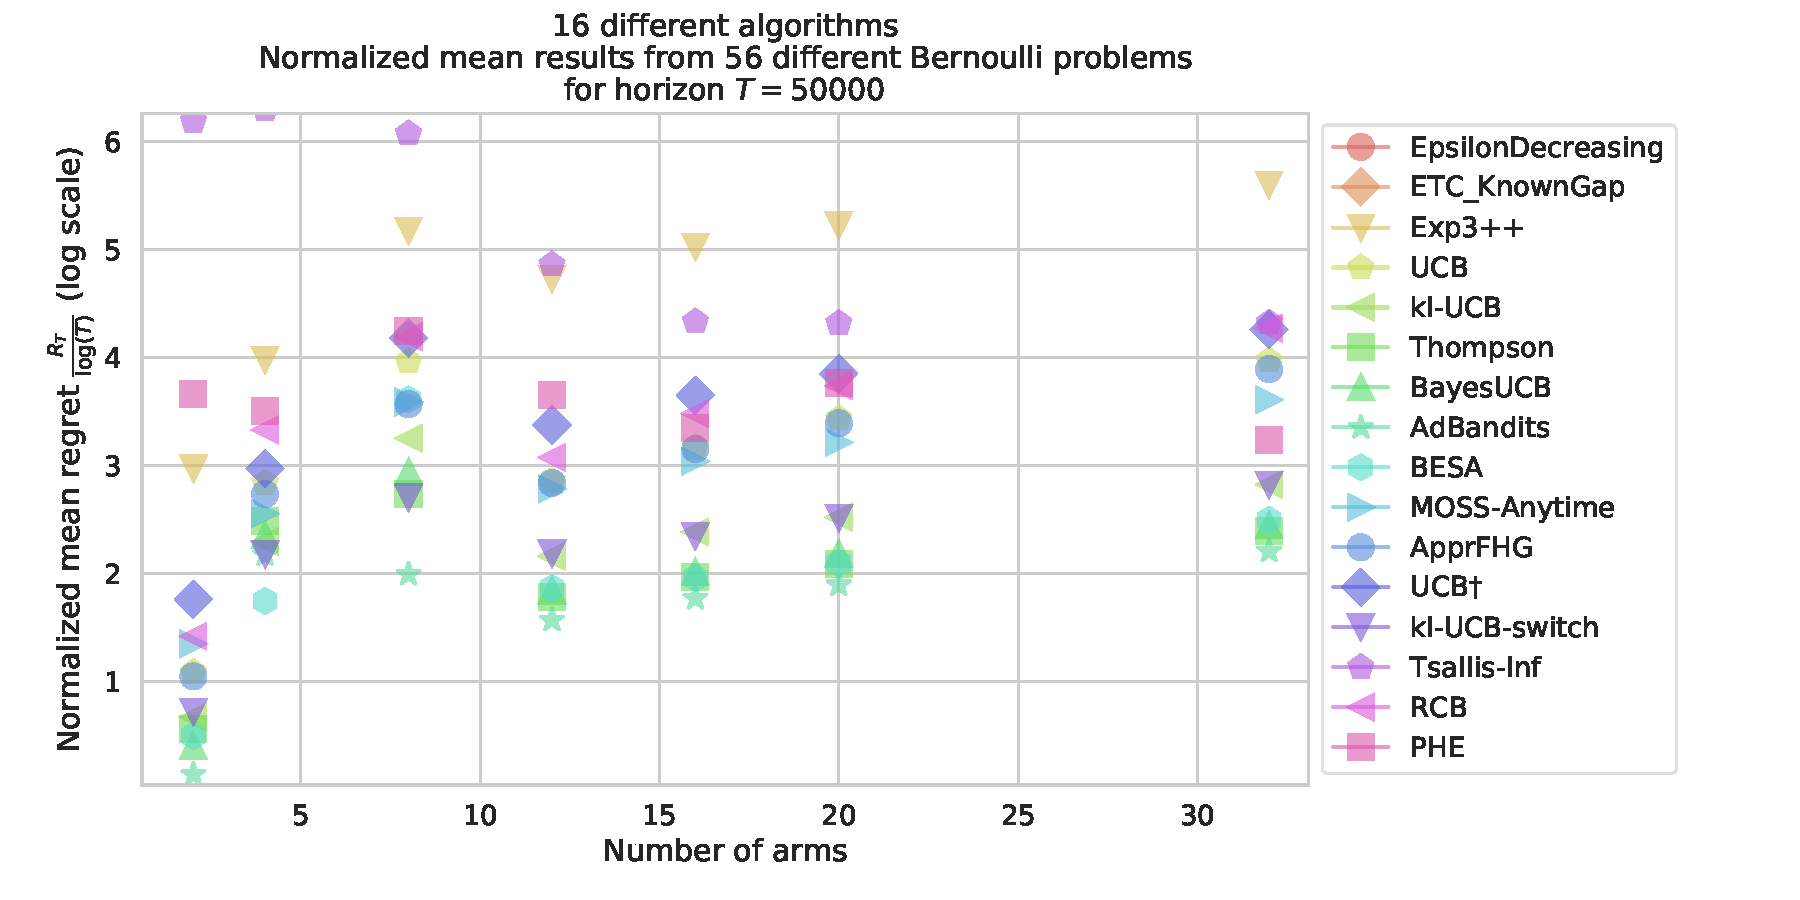
\includegraphics[width=1.10\linewidth]{16_different_algorithms__lognormregret_vs_arms__56pb__7Ks_T50000.pdf}
	\caption[Regret vs different values of $K$.]{
        Regret vs different values of $K$ ($R_T / \log(T)$),
        for $T=50000$ and for $16$ algorithms.
        The $y$-axis is in log-scale.
        All algorithms appear to have a regret slowly growing with respect to $K$, as predicted by the regret bounds which are linear with respect to the number of arms, as predicted.
        \textsc{Tsallis-Inf} is the only state-of-the-art algorithm which appears to be very inefficient for problems with a small number of arms.
        Both the $\varepsilon$-greedy and Explore-then-Commit algorithms performed poorly, achieving linear regret (not displayed).
	}
	\label{fig:3:16_different_algorithms__lognormregret_vs_arms__56pb__7Ks_T50000}
\end{figure}

\begin{figure}[h!]  % [htbp]
	% \centering
	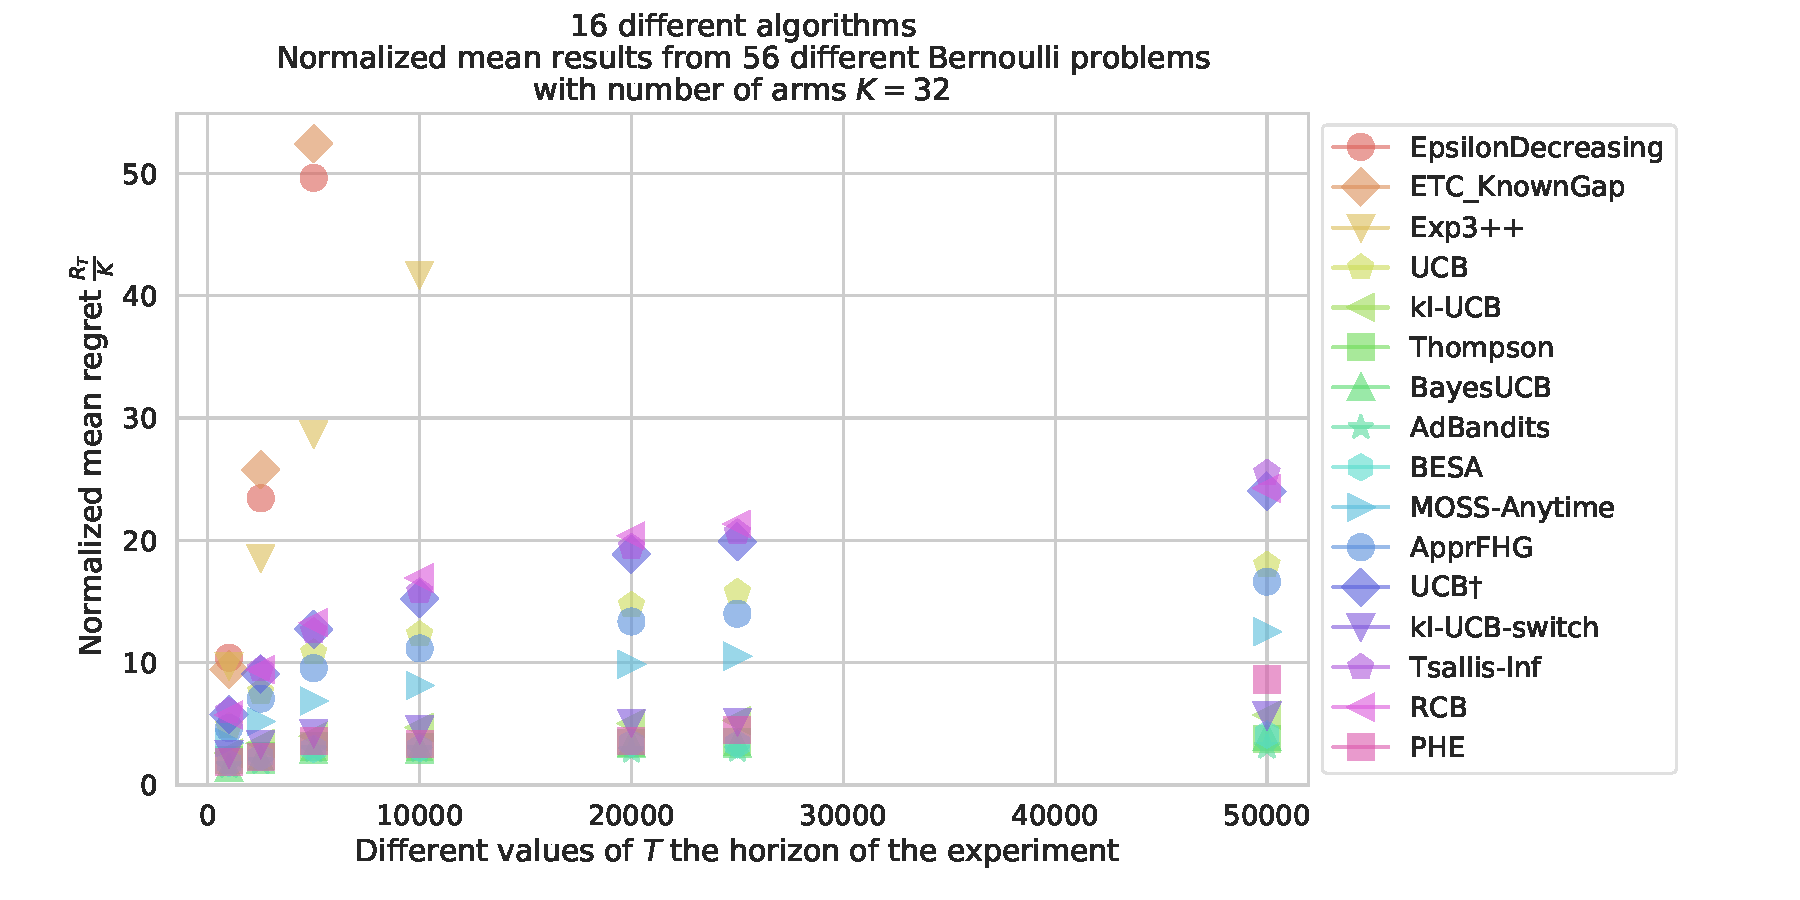
\includegraphics[width=1.10\linewidth]{16_different_algorithms__normregret_vs_horizons__56pb__K32_7Ts.pdf}
	\caption[Regret vs different values of $T$.]{
        Regret vs different values of $T$ ($R_T / K$),
        for $K=32$ and for $16$ algorithms.
        All efficient algorithms appear to have a logarithmic regret, meaning that their regret bound is indeed logarithmic with respect to the horizon, as predicted.
        The respective ranking of all the algorithms also appears to remain preserved for different values of $T$, which is also backed-up by theoretical results: if two algorithms $\cA$ and $\cA'$ has a regret close to their regret bounds, of the form $R_T \leq \cO(K \log(T))$, and the bound for $\cA$ use a smaller constant than the bound for $\cA'$, $\cA$ should obtain a smaller regret than $\cA'$ no matter the horizon.
        Finally, we also observe once more than both the $\varepsilon$-greedy and Explore-then-Commit algorithms performed poorly, achieving linear regret (not displayed after $T=100000$).
	}
	\label{fig:3:16_different_algorithms__normregret_vs_horizons__56pb__K32_7Ts}
\end{figure}


\subsection{Observations and summary of the experiments}

\TODOL{Au lieu d'avoir des longues captions pour les figures, je vais écrire quelques paragraphes donnant les mêmes conclusion et faisant référence aux figures. Je ferai ça très vite si on est contents des figures.}

\TODOL{Use UCB and klUCB, it's enough to be efficient!}
\TODOL{Regret usually scales as $\bigO{K}$ and $\bigO{\log T}$ !}


% I want to show that SMPyBandits contains highly documented implementations of all the most important algorithms designed for stationary single-player multi-armed bandit.

% I will include here formulas about the main algorithms (klUCB, MOSS, etc).
% I will pick some problems (Bernoulli, Gaussian, others), with fixed means or ``Bayesian'' means (\ie, changing at each time) and I will run extensive numerical simulations to compare the main algorithms.

% The take away message is: klUCB beats UCB, Thompson sampling is great too, all the others algorithms are less efficient or comparable, so we only use klUCB for all the rest of this thesis.

% I will include graphs showing the mean regret $R_t$ as a function of time $t$, as well as histograms or boxplots showing the distribution of $R_T$.


% ----------------------------------------------------------------------------
\section{Comparing real measurements of time and memory costs}
\label{sec:3:timeAndMemoryCosts}

\TODOL{Tout ce blabla est un peu trop long, je devrais couper et être plus concis !}

% \TODOL{Write text for this Section, write configuration.py file, run short-term experiment, include them, if happy about it, run longer ang larger experiments}

In this section, we report additional experiment results from the simulations described in the previous Section~\ref{sec:3:reviewSPAlgorithms}.
Instead of studying on the efficiency of the algorithms (\ie, their regret), we report results of real measurements in terms of computational time as well as memory storage.
%
The goal of this section is to verify that the simplest (but most efficient) algorithms have a memory cost proportional to the number of arms but independent of the horizons, \ie, bounded by $\bigO{K}$, and a time complexity at each time step $t\in\{1,\dots,T\}$ bounded by $\bigO{K}$, independent of $t$.

While the results reported in the previous section should not depend on the implementation of the different algorithms, the results in this section concern real measurements of both time and memory consumptions of the simulation software used for these simulations.
Hence, the reported results highly depend on many factors, including how the code is written, and where and when it is run.

\begin{itemize}
    \item Quality and optimization of the code:
    The same level of optimization is used in all the codebase of SMPyBandits, and most of the time, the code is pure and naive Python and was not optimized.
    Mathematical functions (\eg, $\sqrt{\bullet}, \log$) and random numbers used are using \texttt{numpy} and \texttt{numpy.random} modules \cite{numpy}, which are based on C and Cython code \cite{cython} and can be considered highly efficient.
    Computations of Kullback-Leibler and indexes for \klUCB{} algorithms are based on a compiled CPython extension written in C \cite{python} and can also be considered highly efficient.
    As we can safely affirm that the code of the different algorithms has the same level of optimization, the comparison is fair, and we do not favor any algorithm in their implementation in SMPyBandits.

    \item About the experimental environment:
    the exact measurements used for the figures displayed below highly depend on the machine used for the simulation, the version of the language and its libraries (see above in Section~\ref{sub:3:dependencies} for details about SMPyBandits), as well as the number of CPU cores being used (here, we used $12$ cores in a $12$-core desktop) etc.
    As long as the different algorithms and simulations are performed on the same environment, the comparison and conclusions we make from them are fair and do make sense.

\end{itemize}

\paragraph{About the measurement protocol.}
%
To be precise, we used the two following approaches to measure the real time and memory costs of the different algorithms.
\begin{itemize}
    \item For time, we used the \texttt{time.time()} function from Python's standard library, that gives the current time in micro-seconds.
    In the \texttt{Evaluator} object of SMPyBandits, before launching the ``for'' loop on $t\in\{1,\dots,T\}$ for one algorithm, the system time is stored, and when the loop is finished, the time used for this loop is the current system time minus the starting time.
    This measurement gets averaged on the $N=100$ (independent) repetitions, and consistently measure the time efficiency of the algorithms.
    \item For memory, we use two different approaches whether the code runs on a UNIX or a Windows system.
    On UNIX, the \texttt{resource} module allows to measure the memory of the current process, and by counting the difference in memory used by the \texttt{Evaluator} object before and after the ``for'' loop, we can track the memory used by the algorithm to store all its interior variables.
\end{itemize}
In both cases, the ``for'' loop takes some time and stores many variables, but the only difference in terms of both time or memory between two algorithms is explained by the difference in the implementation of the algorithms.
%     def time()
% time() -> floating point number

% Return the current time in seconds since the Epoch. Fractions of a second may be present if the system clock provides them.

% sys.getsizeof(pickle.dumps(policy))
% return resource.getrusage(resource.RUSAGE_SELF).ru_maxrss

\paragraph{Comparing measurements.}
But what is important in these simulation results is not the exact values, but rather to compare the costs of the different algorithms, and thus only the relative difference in terms of time and memory costs are important.
Relative difference for costs do not depend much on the code and the machine used for the simulation.
%
% The tables~\ref{table:3:time_problem1}, \ref{table:3:time_problem2} \ref{table:3:memory_problem1} and \ref{table:3:memory_problem2} below follow the same structure as the ones given in Section~\ref{sec:3:reviewSPAlgorithms} but report results in terms of computation time (in milli-seconds) and memory (in B).
The computation time is \emph{normalized}, that is it is divided by the horizon, to count the (average) time used by an algorithm at time $t$ from $t=1$ to $t=T$, while the memory cost is \emph{not normalized}.
%
Thus, we can check that efficient algorithms have a running time independent on the horizon $T$, instead of just observing a linear dependency, and we can check that efficient algorithms have a memory cost independent on the horizon.
All the considered algorithms in this Chapter are efficient in this aspect, but in Chapter~\ref{chapter:6} we study algorithms that essentially have to store, and run computations, on an increasing number of observations (\eg, \CUSUMUCB), so their computation cost at time $t$ increases (linearly) with $t$, and thus they are more costly.
%
We can also check that efficient algorithms have a running time and a memory cost linear in the number of arms $K$, while more complex algorithms like BESA suffer from an exponential blow-up of their complexity when $K$ increases.


\paragraph{Normalizing data.}
%
The two figures below regret normalized data, in the following way.
For each algorithm, we ran simulations to obtain its (empirical) regret, computation time and space requirement, for different problems with different values of $K$ and $T$.
Simply considering the average of such measurements makes no sense, as for instance two values of the regret for $T=1000$ or $T=50000$ do not have the same order of magnitude.
%
We know that efficient algorithms are expected to follow these patterns:
\begin{itemize}
    \item The final regret $R_T$ should scale as $\cO(K \log(T))$,
    \item The total computation time $\cT_T$ should scale as $\cO(K T)$ (\ie, a computation time of $\cO(K)$ for each time step $t$),
    \item The total memory cost $\cM_T$ should scale as $\cO(K)$, independent of the horizon.
\end{itemize}
Thus, on the first hand, when we show aggregated results from all the different values of $K$ and $T$, we normalized the data by dividing the regrets by $K \log(T)$, the times by $K T$ and the memory by $K$.
%
On the other hand, when we plot a quantity ($R_T$, $\cT_T$, $\cM_T$) as a function of $T$ (resp. of $K$) we only normalize by $K$ (resp. by $T$).


\subsection{Computational time}

% \TODOL{Just one long table for problem 1, not necessary to include other problems}

\begin{figure}[h!]  % [htbp]
	% \centering
	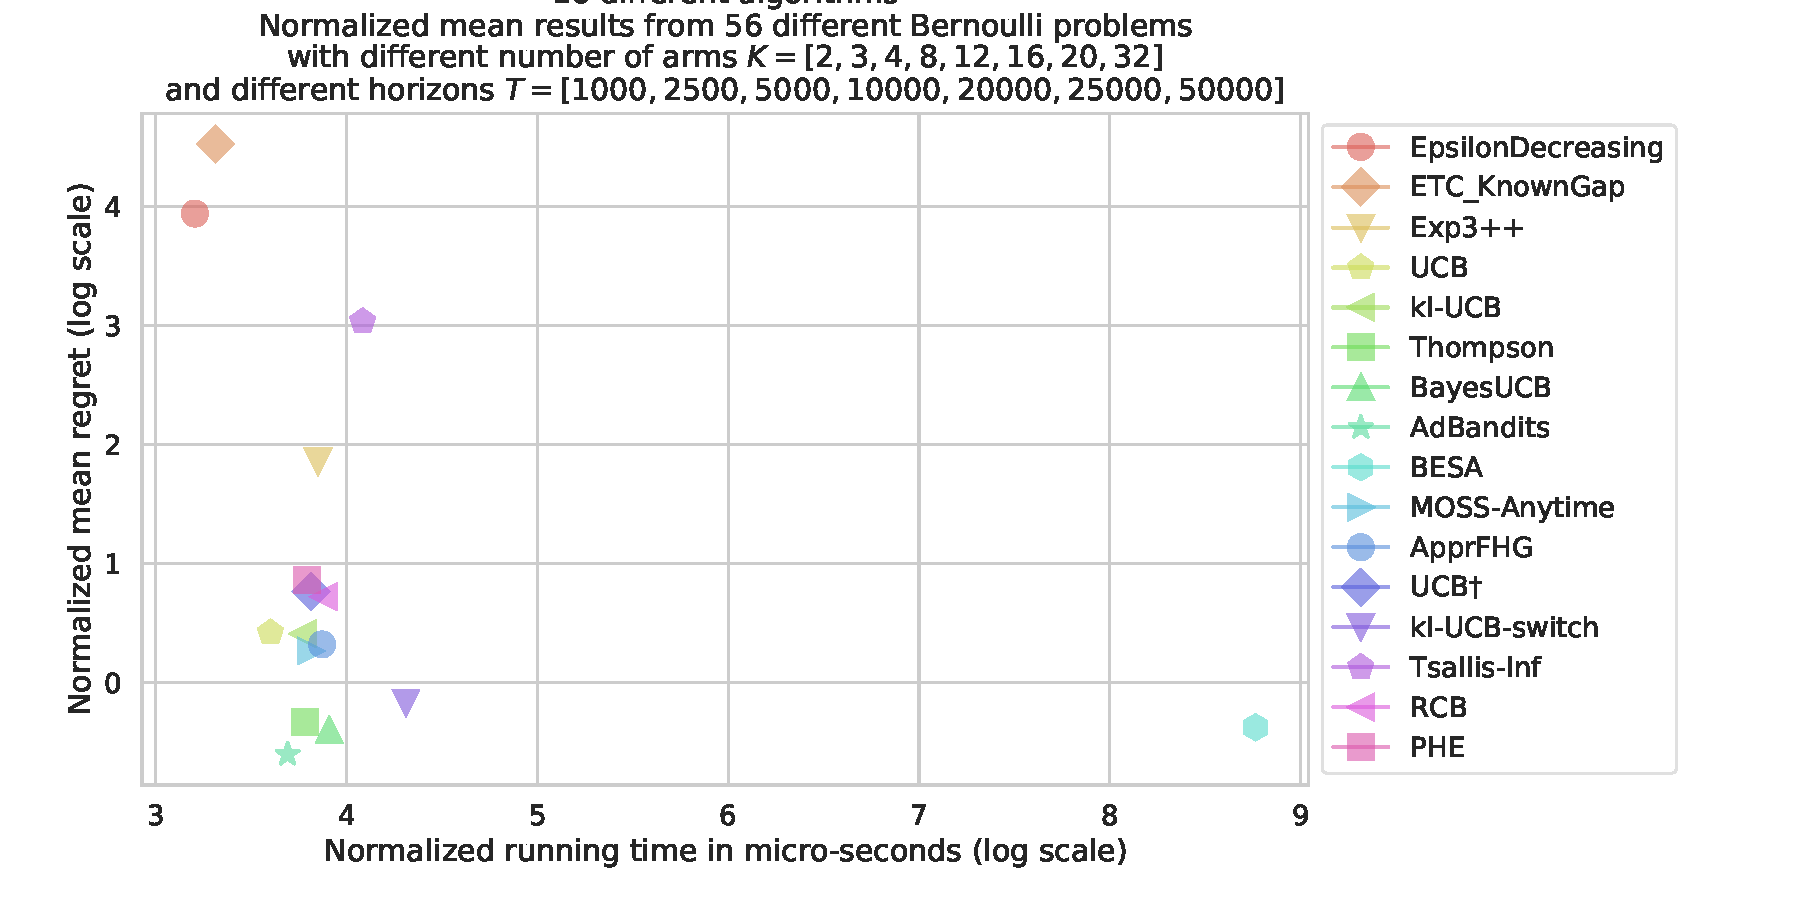
\includegraphics[width=1.10\linewidth]{16_different_algorithms__lognormregret_vs_lognormtime__56pb__7Ks_7Ts.pdf}
	\caption[Normalized mean regret vs normalized running time (in micro-seconds).]{
        Normalized mean regret vs normalized running time (in micro-seconds),
        aggregating the results from different values of $K$ and $T$, for $16$ algorithms.
        Both the $x$-axis and $y$-axis are in log-scale.
        \UCB{} and \klUCB{} are among the best algorithms, while AdBandits, Thompson sampling and Bayes-UCB slightly outperform them in terms of regret, and have similar running times.
	}
	\label{fig:3:16_different_algorithms__lognormregret_vs_lognormtime__56pb__7Ks_7Ts}
\end{figure}


% FIXME generate from the notebook then copy from WS3
\begin{figure}[h!]  % [htbp]
	% \centering
	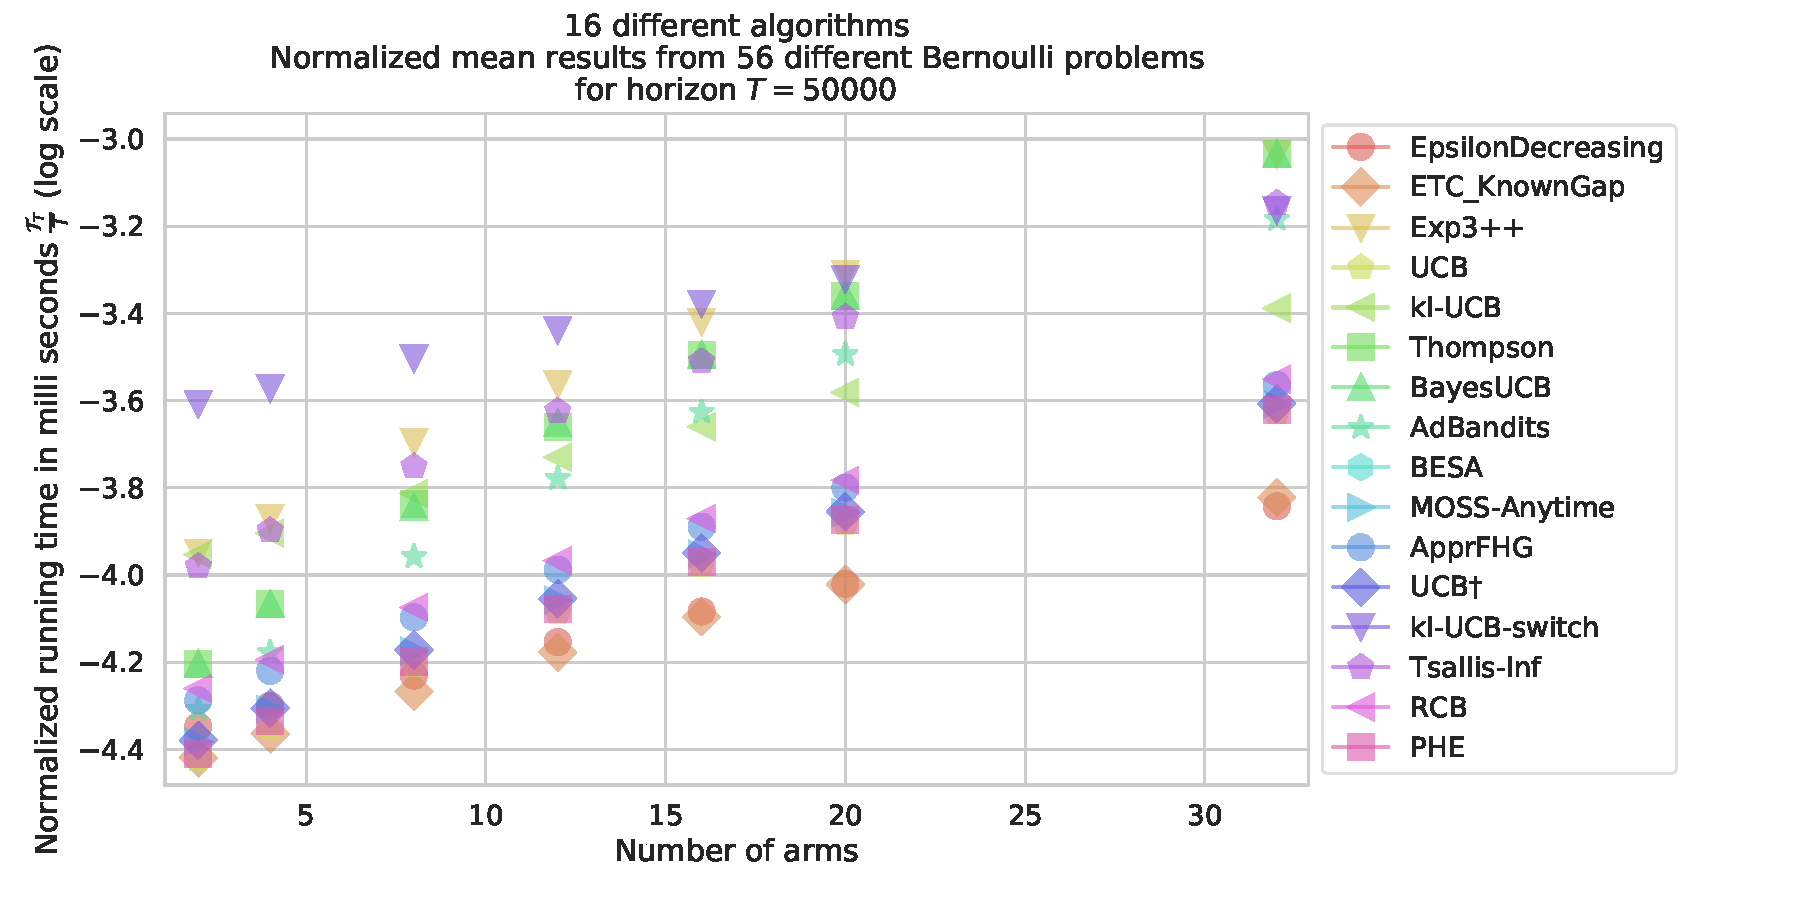
\includegraphics[width=1.10\linewidth]{16_different_algorithms__lognormtime_vs_arms__56pb__7Ks_T50000.pdf}
	\caption[Normalized running time vs different values of $K$.]{
        Normalized running time vs different values of $K$ ($\cT_T / T$),
        for $T=50000$ and for $16$ algorithms.
        $y$-axis is in log-scale.
        All algorithms except BESA has a linear normalized running time, meaning that for $K$ arms they use a computation time proportional to $K$, as predicted.
	}
	\label{fig:3:16_different_algorithms__lognormtime_vs_arms__56pb__7Ks_T50000}
\end{figure}

\begin{figure}[h!]  % [htbp]
	% \centering
	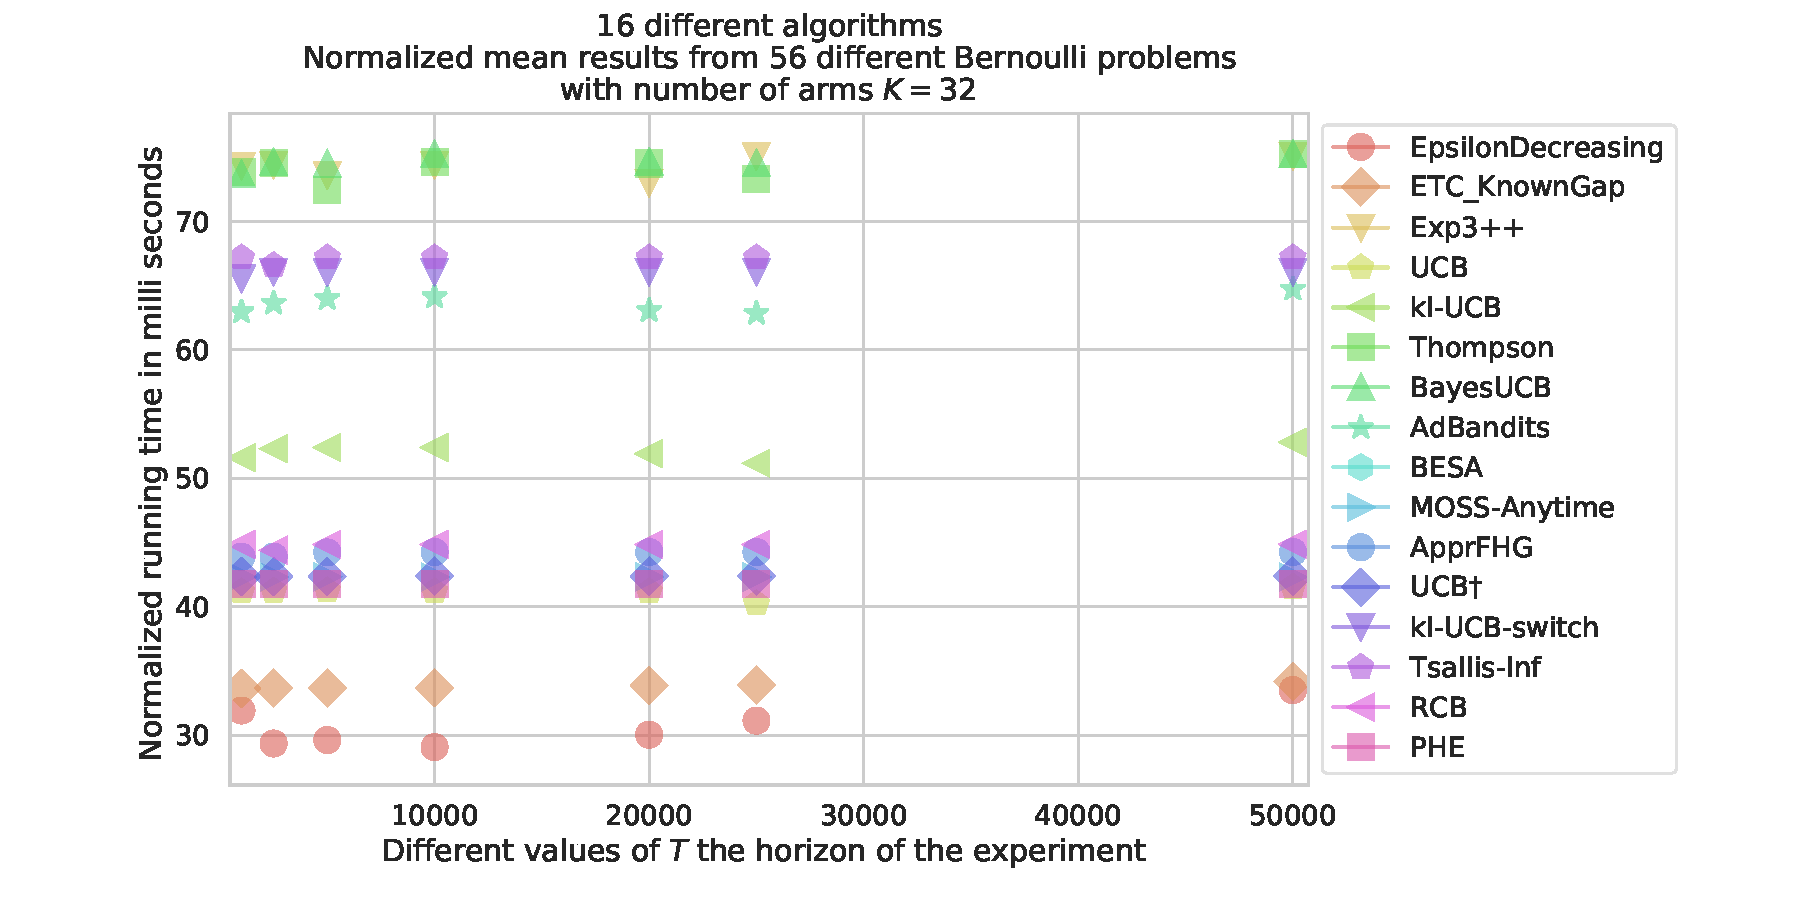
\includegraphics[width=1.10\linewidth]{16_different_algorithms__normtime_vs_horizons__56pb__K32_7Ts.pdf}
	\caption[Normalized running time vs different values of $T$.]{
        Normalized running time vs different values of $T$ ($\cT_T / T$),
        for $K=32$ and for $16$ algorithms.
        All algorithms except BESA has a constant normalized running time, meaning that for $T$ rounds they use a computation time proportional to $T$, as predicted.
	}
	\label{fig:3:16_different_algorithms__normtime_vs_horizons__56pb__K32_7Ts}
\end{figure}


% \begin{table}[!t]
% \begin{footnotesize}  % WARNING
%     \centering
%     \begin{tabular}{c|*{5}{m{2cm}}} % WARNING size ?
%     \textbf{Algorithms} $\;$ \textbackslash $\;$ $\mathbf{T=}$
%         & $T_1 = 1000$ & $T_2 = 5000$ & $T_3 = 10000$ & $T_4 = 50000$ \\
%         \hline
%         $\varepsilon$-greedy &
%             $\cT^{1}_{T_1,K_1} = 0$
%                 $\cT^{1}_{T_1,K_2} = 0$
%                 $\cT^{1}_{T_1,K_3} = 0$
%                 $\cT^{1}_{T_1,K_4} = 0$
%                 $\cT^{1}_{T_1,K_5} = 0$ &
%             $\cT^{1}_{T_2,K_1} = 0$
%                 $\cT^{1}_{T_2,K_2} = 0$
%                 $\cT^{1}_{T_2,K_3} = 0$
%                 $\cT^{1}_{T_2,K_4} = 0$
%                 $\cT^{1}_{T_2,K_5} = 0$ &
%             $\cT^{1}_{T_3,K_1} = 0$
%                 $\cT^{1}_{T_3,K_2} = 0$
%                 $\cT^{1}_{T_3,K_3} = 0$
%                 $\cT^{1}_{T_3,K_4} = 0$
%                 $\cT^{1}_{T_3,K_5} = 0$ &
%             $\cT^{1}_{T_4,K_1} = 0$
%                 $\cT^{1}_{T_4,K_2} = 0$
%                 $\cT^{1}_{T_4,K_3} = 0$
%                 $\cT^{1}_{T_4,K_4} = 0$
%                 $\cT^{1}_{T_4,K_5} = 0$ \\
%         \hline
%         Explore-then-Commit &
%             $\cT^{2}_{T_1,K_1} = 0$
%                 $\cT^{2}_{T_1,K_2} = 0$
%                 $\cT^{2}_{T_1,K_3} = 0$
%                 $\cT^{2}_{T_1,K_4} = 0$
%                 $\cT^{2}_{T_1,K_5} = 0$ &
%             $\cT^{2}_{T_2,K_1} = 0$
%                 $\cT^{2}_{T_2,K_2} = 0$
%                 $\cT^{2}_{T_2,K_3} = 0$
%                 $\cT^{2}_{T_2,K_4} = 0$
%                 $\cT^{2}_{T_2,K_5} = 0$ &
%             $\cT^{2}_{T_3,K_1} = 0$
%                 $\cT^{2}_{T_3,K_2} = 0$
%                 $\cT^{2}_{T_3,K_3} = 0$
%                 $\cT^{2}_{T_3,K_4} = 0$
%                 $\cT^{2}_{T_3,K_5} = 0$ &
%             $\cT^{2}_{T_4,K_1} = 0$
%                 $\cT^{2}_{T_4,K_2} = 0$
%                 $\cT^{2}_{T_4,K_3} = 0$
%                 $\cT^{2}_{T_4,K_4} = 0$
%                 $\cT^{2}_{T_4,K_5} = 0$ \\
%         \hline
%         $\mathrm{Exp}3^{++}$ &
%             $\cT^3_{T_1,K_1} = 0$
%                 $\cT^3_{T_1,K_2} = 0$
%                 $\cT^3_{T_1,K_3} = 0$
%                 $\cT^3_{T_1,K_4} = 0$
%                 $\cT^3_{T_1,K_5} = 0$ &
%             $\cT^3_{T_2,K_1} = 0$
%                 $\cT^3_{T_2,K_2} = 0$
%                 $\cT^3_{T_2,K_3} = 0$
%                 $\cT^3_{T_2,K_4} = 0$
%                 $\cT^3_{T_2,K_5} = 0$ &
%             $\cT^3_{T_3,K_1} = 0$
%                 $\cT^3_{T_3,K_2} = 0$
%                 $\cT^3_{T_3,K_3} = 0$
%                 $\cT^3_{T_3,K_4} = 0$
%                 $\cT^3_{T_3,K_5} = 0$ &
%             $\cT^3_{T_4,K_1} = 0$
%                 $\cT^3_{T_4,K_2} = 0$
%                 $\cT^3_{T_4,K_3} = 0$
%                 $\cT^3_{T_4,K_4} = 0$
%                 $\cT^3_{T_4,K_5} = 0$ \\
%         \hline
%         $\UCB_1$ &
%             $\cT^{4}_{T_1,K_1} = 0$
%                 $\cT^{4}_{T_1,K_2} = 0$
%                 $\cT^{4}_{T_1,K_3} = 0$
%                 $\cT^{4}_{T_1,K_4} = 0$
%                 $\cT^{4}_{T_1,K_5} = 0$ &
%             $\cT^{4}_{T_2,K_1} = 0$
%                 $\cT^{4}_{T_2,K_2} = 0$
%                 $\cT^{4}_{T_2,K_3} = 0$
%                 $\cT^{4}_{T_2,K_4} = 0$
%                 $\cT^{4}_{T_2,K_5} = 0$ &
%             $\cT^{4}_{T_3,K_1} = 0$
%                 $\cT^{4}_{T_3,K_2} = 0$
%                 $\cT^{4}_{T_3,K_3} = 0$
%                 $\cT^{4}_{T_3,K_4} = 0$
%                 $\cT^{4}_{T_3,K_5} = 0$ &
%             $\cT^{4}_{T_4,K_1} = 0$
%                 $\cT^{4}_{T_4,K_2} = 0$
%                 $\cT^{4}_{T_4,K_3} = 0$
%                 $\cT^{4}_{T_4,K_4} = 0$
%                 $\cT^{4}_{T_4,K_5} = 0$ \\
%         \hline
%         \klUCB{} &
%             $\cT^{5}_{T_1,K_1} = 0$
%                 $\cT^{5}_{T_1,K_2} = 0$
%                 $\cT^{5}_{T_1,K_3} = 0$
%                 $\cT^{5}_{T_1,K_4} = 0$
%                 $\cT^{5}_{T_1,K_5} = 0$ &
%             $\cT^{5}_{T_2,K_1} = 0$
%                 $\cT^{5}_{T_2,K_2} = 0$
%                 $\cT^{5}_{T_2,K_3} = 0$
%                 $\cT^{5}_{T_2,K_4} = 0$
%                 $\cT^{5}_{T_2,K_5} = 0$ &
%             $\cT^{5}_{T_3,K_1} = 0$
%                 $\cT^{5}_{T_3,K_2} = 0$
%                 $\cT^{5}_{T_3,K_3} = 0$
%                 $\cT^{5}_{T_3,K_4} = 0$
%                 $\cT^{5}_{T_3,K_5} = 0$ &
%             $\cT^{5}_{T_4,K_1} = 0$
%                 $\cT^{5}_{T_4,K_2} = 0$
%                 $\cT^{5}_{T_4,K_3} = 0$
%                 $\cT^{5}_{T_4,K_4} = 0$
%                 $\cT^{5}_{T_4,K_5} = 0$ \\
%         \hline
%         Thompson sampling &
%             $\cT^{6}_{T_1,K_1} = 0$
%                 $\cT^{6}_{T_1,K_2} = 0$
%                 $\cT^{6}_{T_1,K_3} = 0$
%                 $\cT^{6}_{T_1,K_4} = 0$
%                 $\cT^{6}_{T_1,K_5} = 0$ &
%             $\cT^{6}_{T_2,K_1} = 0$
%                 $\cT^{6}_{T_2,K_2} = 0$
%                 $\cT^{6}_{T_2,K_3} = 0$
%                 $\cT^{6}_{T_2,K_4} = 0$
%                 $\cT^{6}_{T_2,K_5} = 0$ &
%             $\cT^{6}_{T_3,K_1} = 0$
%                 $\cT^{6}_{T_3,K_2} = 0$
%                 $\cT^{6}_{T_3,K_3} = 0$
%                 $\cT^{6}_{T_3,K_4} = 0$
%                 $\cT^{6}_{T_3,K_5} = 0$ &
%             $\cT^{6}_{T_4,K_1} = 0$
%                 $\cT^{6}_{T_4,K_2} = 0$
%                 $\cT^{6}_{T_4,K_3} = 0$
%                 $\cT^{6}_{T_4,K_4} = 0$
%                 $\cT^{6}_{T_4,K_5} = 0$ \\
%         \hline
%         Thompson sampling &
%             $\cT^{7}_{T_1,K_1} = 0$
%                 $\cT^{7}_{T_1,K_2} = 0$
%                 $\cT^{7}_{T_1,K_3} = 0$
%                 $\cT^{7}_{T_1,K_4} = 0$
%                 $\cT^{7}_{T_1,K_5} = 0$ &
%             $\cT^{7}_{T_2,K_1} = 0$
%                 $\cT^{7}_{T_2,K_2} = 0$
%                 $\cT^{7}_{T_2,K_3} = 0$
%                 $\cT^{7}_{T_2,K_4} = 0$
%                 $\cT^{7}_{T_2,K_5} = 0$ &
%             $\cT^{7}_{T_3,K_1} = 0$
%                 $\cT^{7}_{T_3,K_2} = 0$
%                 $\cT^{7}_{T_3,K_3} = 0$
%                 $\cT^{7}_{T_3,K_4} = 0$
%                 $\cT^{7}_{T_3,K_5} = 0$ &
%             $\cT^{7}_{T_4,K_1} = 0$
%                 $\cT^{7}_{T_4,K_2} = 0$
%                 $\cT^{7}_{T_4,K_3} = 0$
%                 $\cT^{7}_{T_4,K_4} = 0$
%                 $\cT^{7}_{T_4,K_5} = 0$ \\
%         \hline
%         AdBandits &
%             $\cT^{8}_{T_1,K_1} = 0$
%                 $\cT^{8}_{T_1,K_2} = 0$
%                 $\cT^{8}_{T_1,K_3} = 0$
%                 $\cT^{8}_{T_1,K_4} = 0$
%                 $\cT^{8}_{T_1,K_5} = 0$ &
%             $\cT^{8}_{T_2,K_1} = 0$
%                 $\cT^{8}_{T_2,K_2} = 0$
%                 $\cT^{8}_{T_2,K_3} = 0$
%                 $\cT^{8}_{T_2,K_4} = 0$
%                 $\cT^{8}_{T_2,K_5} = 0$ &
%             $\cT^{8}_{T_3,K_1} = 0$
%                 $\cT^{8}_{T_3,K_2} = 0$
%                 $\cT^{8}_{T_3,K_3} = 0$
%                 $\cT^{8}_{T_3,K_4} = 0$
%                 $\cT^{8}_{T_3,K_5} = 0$ &
%             $\cT^{8}_{T_4,K_1} = 0$
%                 $\cT^{8}_{T_4,K_2} = 0$
%                 $\cT^{8}_{T_4,K_3} = 0$
%                 $\cT^{8}_{T_4,K_4} = 0$
%                 $\cT^{8}_{T_4,K_5} = 0$ \\
%         \hline
%         BESA &
%             $\cT^{9}_{T_1,K_1} = 0$
%                 $\cT^{9}_{T_1,K_2} = 0$
%                 $\cT^{9}_{T_1,K_3} = 0$
%                 $\cT^{9}_{T_1,K_4} = 0$
%                 $\cT^{9}_{T_1,K_5} = 0$ &
%             $\cT^{9}_{T_2,K_1} = 0$
%                 $\cT^{9}_{T_2,K_2} = 0$
%                 $\cT^{9}_{T_2,K_3} = 0$
%                 $\cT^{9}_{T_2,K_4} = 0$
%                 $\cT^{9}_{T_2,K_5} = 0$ &
%             $\cT^{9}_{T_3,K_1} = 0$
%                 $\cT^{9}_{T_3,K_2} = 0$
%                 $\cT^{9}_{T_3,K_3} = 0$
%                 $\cT^{9}_{T_3,K_4} = 0$
%                 $\cT^{9}_{T_3,K_5} = 0$ &
%             $\cT^{9}_{T_4,K_1} = 0$
%                 $\cT^{9}_{T_4,K_2} = 0$
%                 $\cT^{9}_{T_4,K_3} = 0$
%                 $\cT^{9}_{T_4,K_4} = 0$
%                 $\cT^{9}_{T_4,K_5} = 0$ \\
%         \hline
%     \end{tabular}
%     \caption{Normalized running time, rounded and in milli-seconds, for $9$ different algorithms on problem $1$ with different, values of time $T$ and number of arm $K$.}
%     \label{table:3:time_problem1}
% \end{footnotesize}  % WARNING
% \end{table}


\subsection{Memory cost}

% \TODOL{Just one long table for problem 1, not necessary to include other problems}

\begin{figure}[h!]  % [htbp]
	% \centering
	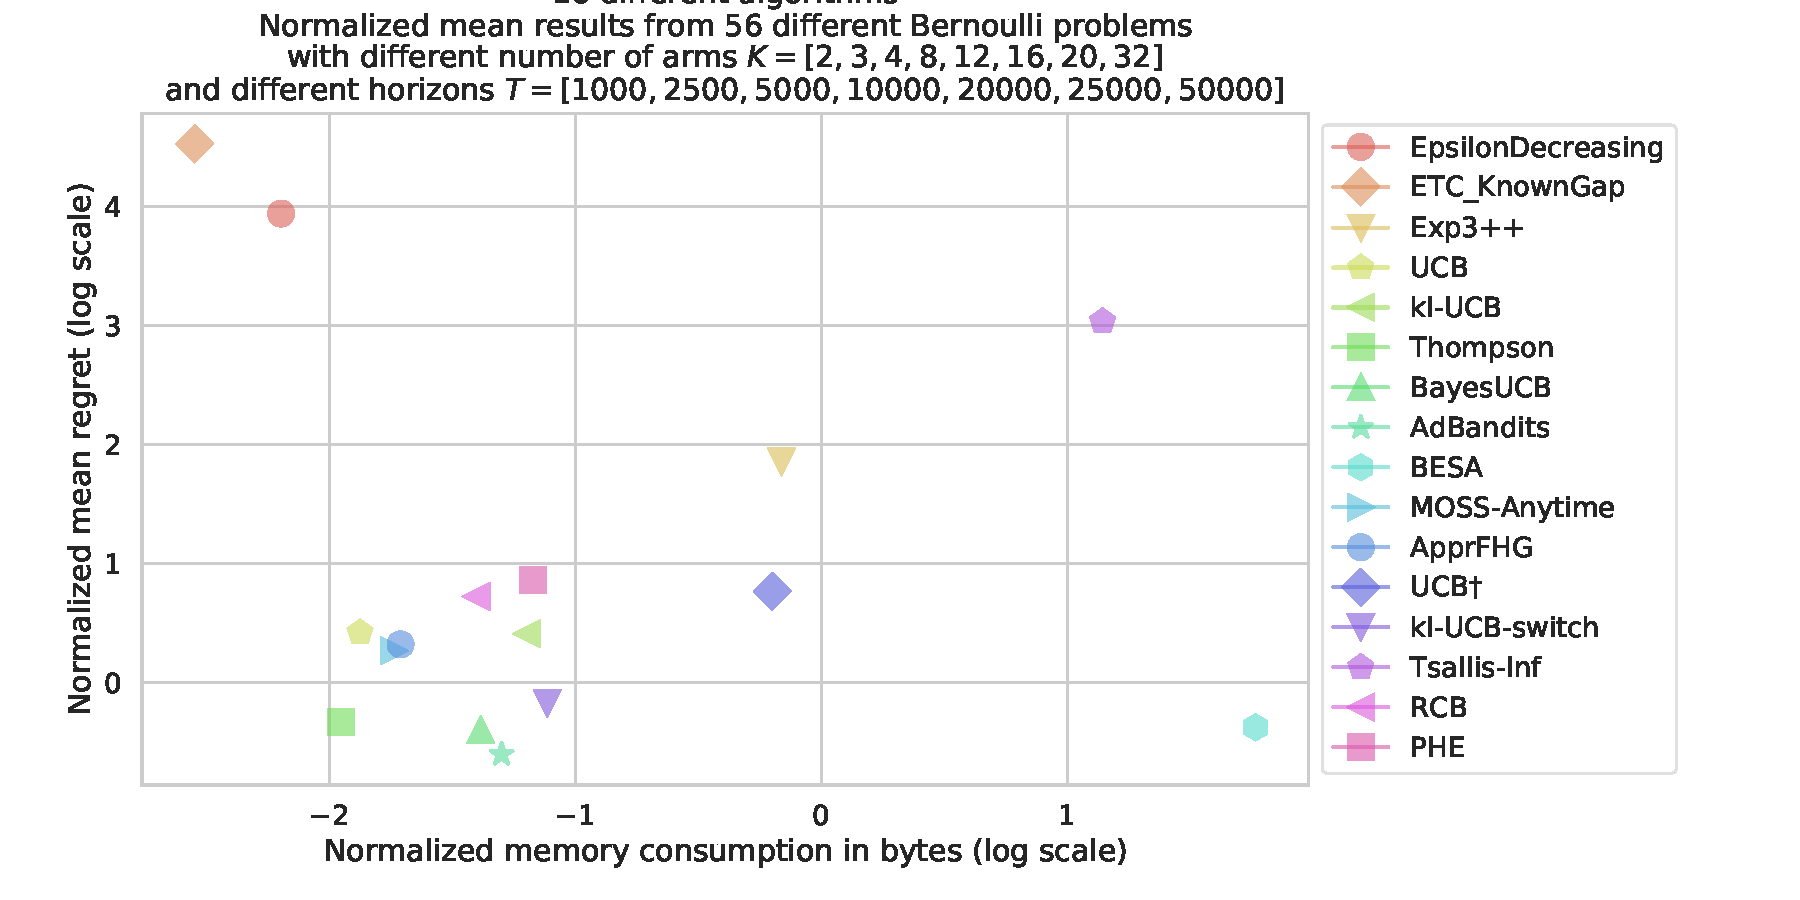
\includegraphics[width=1.10\linewidth]{16_different_algorithms__lognormregret_vs_lognormmemory__56pb__7Ks_7Ts.pdf}
	\caption[Normalized mean regret vs normalized memory costs (in bytes).]{
        Normalized mean regret vs normalized memory costs (in bytes),
        aggregating the results from different values of $K$ and $T$, for $16$ algorithms.
        Both the $x$-axis and $y$-axis are in log-scale.
        Thompson sampling appears as the best algorithm in this visualization, while \UCB{} has the advantage of being memory efficient, and \klUCB{} obtains similar performances.
	}
	\label{fig:3:16_different_algorithms__lognormregret_vs_lognormmemory__56pb__7Ks_7Ts}
\end{figure}


% FIXME generate from the notebook then copy from WS3
\begin{figure}[h!]  % [htbp]
	% \centering
	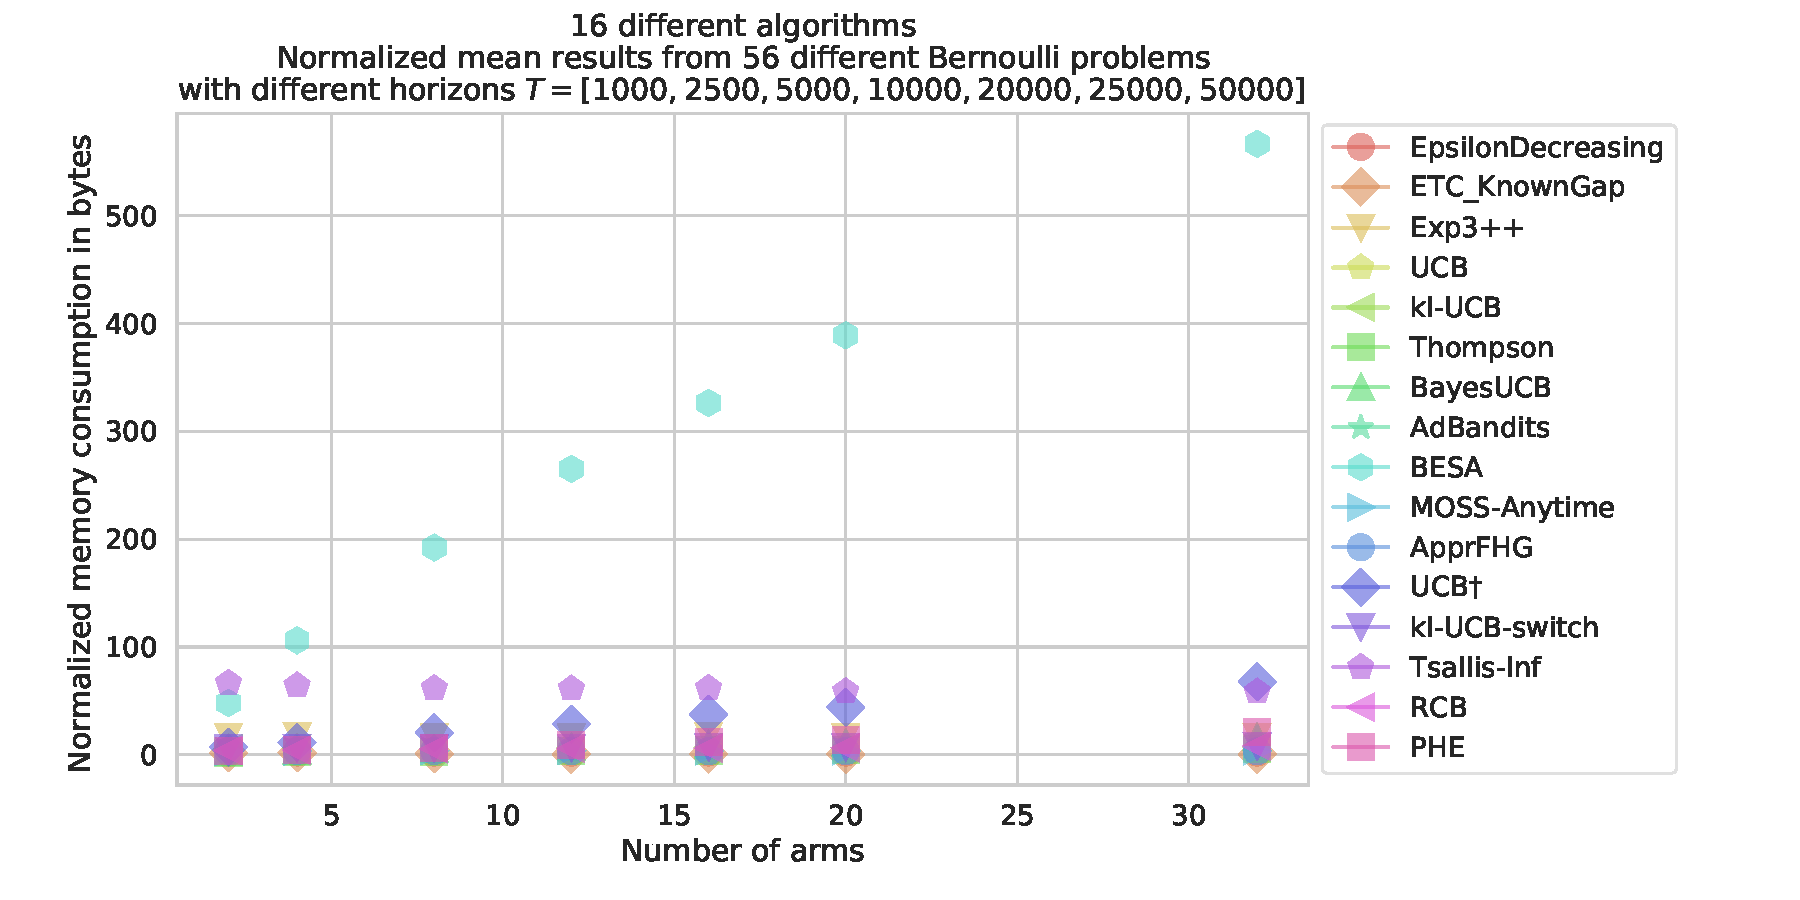
\includegraphics[width=1.10\linewidth]{16_different_algorithms__normmemory_vs_arms__56pb__7Ks_T50000.pdf}
	\caption[Normalized memory cost vs different values of $K$.]{
        Normalized memory cost vs different values of $K$ ($\cM_T / K$),
        for $T=50000$ and for $16$ algorithms.
        % $y$-axis is in log-scale.
        All algorithms (except BESA) has an almost constant memory cost, meaning that for $K$ arms they use a storage proportional to $K$, as predicted.
	}
	\label{fig:3:16_different_algorithms__normmemory_vs_arms__56pb__7Ks_T50000}
\end{figure}

\begin{figure}[h!]  % [htbp]
	% \centering
	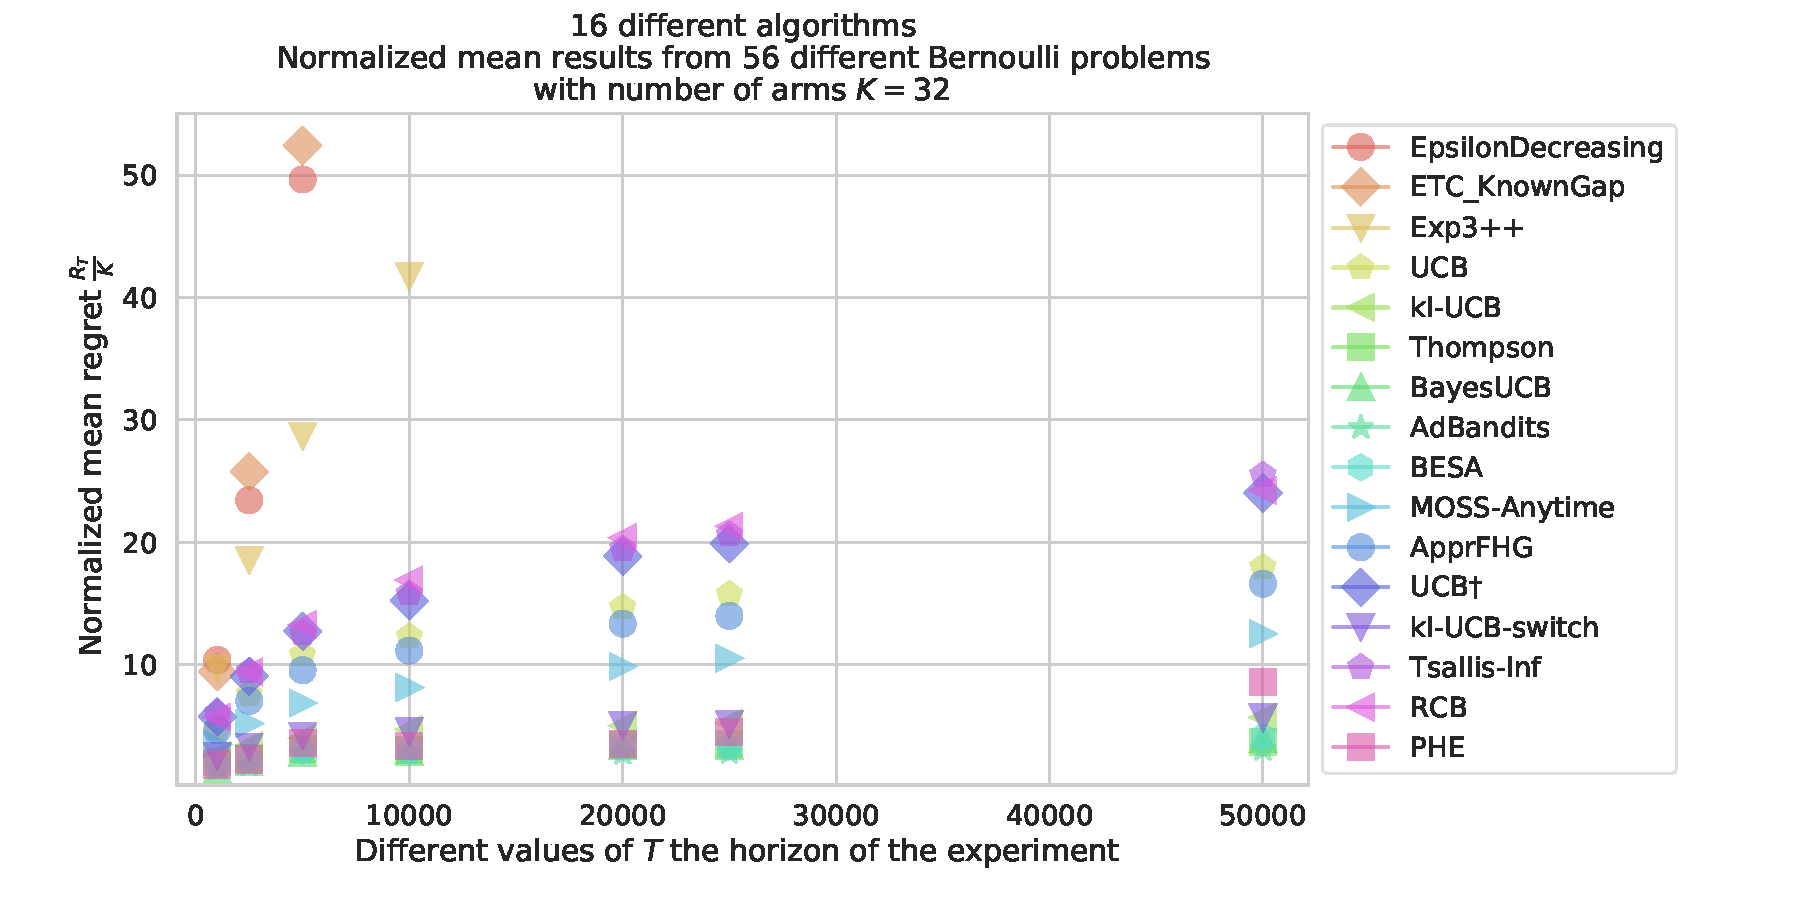
\includegraphics[width=1.10\linewidth]{16_different_algorithms__normmemory_vs_horizons__56pb__K32_7Ts.pdf}
	\caption[Normalized memory cost vs different values of $T$.]{
        Normalized memory cost vs different values of $T$ ($\cM_T / K$),
        for $K=32$ and for $16$ algorithms.
        All algorithms (except BESA) has a very slowly growing normalized memory cost, meaning that for $T$ rounds they use a computation time almost independent of $T$, as predicted.
        There is a clear separation between three groups.
        First, BESA is very costly in terms of memory, and $\UCB\dagger$ and \textsc{Tsallis-Inf} are also more costly than others, and both experiences a linear growth of their memory cost.
        Then, we see PHE, $\mathrm{Exp}3++$, Bayes-UCB and AdBandits having a small but linear growth of memory cost, and it can be explained for each of them (\eg, for Bayes-UCB, computing the $1-1/t$ quantile at time $t$ becomes more and more costly as $t$ grows, and thus as $T$ grows,  ).
        Finally, the other algorithms (including \UCB, \klUCB{} and Thompson sampling) have a very small footprint and their memory cost do not grow much when $T$ increases.
	}
	\label{fig:3:16_different_algorithms__normmemory_vs_horizons__56pb__K32_7Ts}
\end{figure}


% \begin{table}[!t]
% \begin{footnotesize}  % WARNING
%     \centering
%     \begin{tabular}{c|*{5}{m{2cm}}} % WARNING size ?
%     \textbf{Algorithms} $\;$ \textbackslash $\;$ $\mathbf{T=}$
%         & $T_1 = 1000$ & $T_2 = 5000$ & $T_3 = 10000$ & $T_4 = 50000$ \\
%         \hline
%         $\varepsilon$-greedy &
%             $\cM^{1}_{T_1,K_1} = 0$
%                 $\cM^{1}_{T_1,K_2} = 0$
%                 $\cM^{1}_{T_1,K_3} = 0$
%                 $\cM^{1}_{T_1,K_4} = 0$
%                 $\cM^{1}_{T_1,K_5} = 0$ &
%             $\cM^{1}_{T_2,K_1} = 0$
%                 $\cM^{1}_{T_2,K_2} = 0$
%                 $\cM^{1}_{T_2,K_3} = 0$
%                 $\cM^{1}_{T_2,K_4} = 0$
%                 $\cM^{1}_{T_2,K_5} = 0$ &
%             $\cM^{1}_{T_3,K_1} = 0$
%                 $\cM^{1}_{T_3,K_2} = 0$
%                 $\cM^{1}_{T_3,K_3} = 0$
%                 $\cM^{1}_{T_3,K_4} = 0$
%                 $\cM^{1}_{T_3,K_5} = 0$ &
%             $\cM^{1}_{T_4,K_1} = 0$
%                 $\cM^{1}_{T_4,K_2} = 0$
%                 $\cM^{1}_{T_4,K_3} = 0$
%                 $\cM^{1}_{T_4,K_4} = 0$
%                 $\cM^{1}_{T_4,K_5} = 0$ \\
%         \hline
%         Explore-then-Commit &
%             $\cM^{2}_{T_1,K_1} = 0$
%                 $\cM^{2}_{T_1,K_2} = 0$
%                 $\cM^{2}_{T_1,K_3} = 0$
%                 $\cM^{2}_{T_1,K_4} = 0$
%                 $\cM^{2}_{T_1,K_5} = 0$ &
%             $\cM^{2}_{T_2,K_1} = 0$
%                 $\cM^{2}_{T_2,K_2} = 0$
%                 $\cM^{2}_{T_2,K_3} = 0$
%                 $\cM^{2}_{T_2,K_4} = 0$
%                 $\cM^{2}_{T_2,K_5} = 0$ &
%             $\cM^{2}_{T_3,K_1} = 0$
%                 $\cM^{2}_{T_3,K_2} = 0$
%                 $\cM^{2}_{T_3,K_3} = 0$
%                 $\cM^{2}_{T_3,K_4} = 0$
%                 $\cM^{2}_{T_3,K_5} = 0$ &
%             $\cM^{2}_{T_4,K_1} = 0$
%                 $\cM^{2}_{T_4,K_2} = 0$
%                 $\cM^{2}_{T_4,K_3} = 0$
%                 $\cM^{2}_{T_4,K_4} = 0$
%                 $\cM^{2}_{T_4,K_5} = 0$ \\
%         \hline
%         $\mathrm{Exp}3^{++}$ &
%             $\cM^3_{T_1,K_1} = 0$
%                 $\cM^3_{T_1,K_2} = 0$
%                 $\cM^3_{T_1,K_3} = 0$
%                 $\cM^3_{T_1,K_4} = 0$
%                 $\cM^3_{T_1,K_5} = 0$ &
%             $\cM^3_{T_2,K_1} = 0$
%                 $\cM^3_{T_2,K_2} = 0$
%                 $\cM^3_{T_2,K_3} = 0$
%                 $\cM^3_{T_2,K_4} = 0$
%                 $\cM^3_{T_2,K_5} = 0$ &
%             $\cM^3_{T_3,K_1} = 0$
%                 $\cM^3_{T_3,K_2} = 0$
%                 $\cM^3_{T_3,K_3} = 0$
%                 $\cM^3_{T_3,K_4} = 0$
%                 $\cM^3_{T_3,K_5} = 0$ &
%             $\cM^3_{T_4,K_1} = 0$
%                 $\cM^3_{T_4,K_2} = 0$
%                 $\cM^3_{T_4,K_3} = 0$
%                 $\cM^3_{T_4,K_4} = 0$
%                 $\cM^3_{T_4,K_5} = 0$ \\
%         \hline
%         $\UCB_1$ &
%             $\cM^{4}_{T_1,K_1} = 0$
%                 $\cM^{4}_{T_1,K_2} = 0$
%                 $\cM^{4}_{T_1,K_3} = 0$
%                 $\cM^{4}_{T_1,K_4} = 0$
%                 $\cM^{4}_{T_1,K_5} = 0$ &
%             $\cM^{4}_{T_2,K_1} = 0$
%                 $\cM^{4}_{T_2,K_2} = 0$
%                 $\cM^{4}_{T_2,K_3} = 0$
%                 $\cM^{4}_{T_2,K_4} = 0$
%                 $\cM^{4}_{T_2,K_5} = 0$ &
%             $\cM^{4}_{T_3,K_1} = 0$
%                 $\cM^{4}_{T_3,K_2} = 0$
%                 $\cM^{4}_{T_3,K_3} = 0$
%                 $\cM^{4}_{T_3,K_4} = 0$
%                 $\cM^{4}_{T_3,K_5} = 0$ &
%             $\cM^{4}_{T_4,K_1} = 0$
%                 $\cM^{4}_{T_4,K_2} = 0$
%                 $\cM^{4}_{T_4,K_3} = 0$
%                 $\cM^{4}_{T_4,K_4} = 0$
%                 $\cM^{4}_{T_4,K_5} = 0$ \\
%         \hline
%         \klUCB{} &
%             $\cM^{5}_{T_1,K_1} = 0$
%                 $\cM^{5}_{T_1,K_2} = 0$
%                 $\cM^{5}_{T_1,K_3} = 0$
%                 $\cM^{5}_{T_1,K_4} = 0$
%                 $\cM^{5}_{T_1,K_5} = 0$ &
%             $\cM^{5}_{T_2,K_1} = 0$
%                 $\cM^{5}_{T_2,K_2} = 0$
%                 $\cM^{5}_{T_2,K_3} = 0$
%                 $\cM^{5}_{T_2,K_4} = 0$
%                 $\cM^{5}_{T_2,K_5} = 0$ &
%             $\cM^{5}_{T_3,K_1} = 0$
%                 $\cM^{5}_{T_3,K_2} = 0$
%                 $\cM^{5}_{T_3,K_3} = 0$
%                 $\cM^{5}_{T_3,K_4} = 0$
%                 $\cM^{5}_{T_3,K_5} = 0$ &
%             $\cM^{5}_{T_4,K_1} = 0$
%                 $\cM^{5}_{T_4,K_2} = 0$
%                 $\cM^{5}_{T_4,K_3} = 0$
%                 $\cM^{5}_{T_4,K_4} = 0$
%                 $\cM^{5}_{T_4,K_5} = 0$ \\
%         \hline
%         Thompson sampling &
%             $\cM^{6}_{T_1,K_1} = 0$
%                 $\cM^{6}_{T_1,K_2} = 0$
%                 $\cM^{6}_{T_1,K_3} = 0$
%                 $\cM^{6}_{T_1,K_4} = 0$
%                 $\cM^{6}_{T_1,K_5} = 0$ &
%             $\cM^{6}_{T_2,K_1} = 0$
%                 $\cM^{6}_{T_2,K_2} = 0$
%                 $\cM^{6}_{T_2,K_3} = 0$
%                 $\cM^{6}_{T_2,K_4} = 0$
%                 $\cM^{6}_{T_2,K_5} = 0$ &
%             $\cM^{6}_{T_3,K_1} = 0$
%                 $\cM^{6}_{T_3,K_2} = 0$
%                 $\cM^{6}_{T_3,K_3} = 0$
%                 $\cM^{6}_{T_3,K_4} = 0$
%                 $\cM^{6}_{T_3,K_5} = 0$ &
%             $\cM^{6}_{T_4,K_1} = 0$
%                 $\cM^{6}_{T_4,K_2} = 0$
%                 $\cM^{6}_{T_4,K_3} = 0$
%                 $\cM^{6}_{T_4,K_4} = 0$
%                 $\cM^{6}_{T_4,K_5} = 0$ \\
%         \hline
%         Bayes-UCB &
%             $\cM^{7}_{T_1,K_1} = 0$
%                 $\cM^{7}_{T_1,K_2} = 0$
%                 $\cM^{7}_{T_1,K_3} = 0$
%                 $\cM^{7}_{T_1,K_4} = 0$
%                 $\cM^{7}_{T_1,K_5} = 0$ &
%             $\cM^{7}_{T_2,K_1} = 0$
%                 $\cM^{7}_{T_2,K_2} = 0$
%                 $\cM^{7}_{T_2,K_3} = 0$
%                 $\cM^{7}_{T_2,K_4} = 0$
%                 $\cM^{7}_{T_2,K_5} = 0$ &
%             $\cM^{7}_{T_3,K_1} = 0$
%                 $\cM^{7}_{T_3,K_2} = 0$
%                 $\cM^{7}_{T_3,K_3} = 0$
%                 $\cM^{7}_{T_3,K_4} = 0$
%                 $\cM^{7}_{T_3,K_5} = 0$ &
%             $\cM^{7}_{T_4,K_1} = 0$
%                 $\cM^{7}_{T_4,K_2} = 0$
%                 $\cM^{7}_{T_4,K_3} = 0$
%                 $\cM^{7}_{T_4,K_4} = 0$
%                 $\cM^{7}_{T_4,K_5} = 0$ \\
%         \hline
%         AdBandits &
%             $\cM^{8}_{T_1,K_1} = 0$
%                 $\cM^{8}_{T_1,K_2} = 0$
%                 $\cM^{8}_{T_1,K_3} = 0$
%                 $\cM^{8}_{T_1,K_4} = 0$
%                 $\cM^{8}_{T_1,K_5} = 0$ &
%             $\cM^{8}_{T_2,K_1} = 0$
%                 $\cM^{8}_{T_2,K_2} = 0$
%                 $\cM^{8}_{T_2,K_3} = 0$
%                 $\cM^{8}_{T_2,K_4} = 0$
%                 $\cM^{8}_{T_2,K_5} = 0$ &
%             $\cM^{8}_{T_3,K_1} = 0$
%                 $\cM^{8}_{T_3,K_2} = 0$
%                 $\cM^{8}_{T_3,K_3} = 0$
%                 $\cM^{8}_{T_3,K_4} = 0$
%                 $\cM^{8}_{T_3,K_5} = 0$ &
%             $\cM^{8}_{T_4,K_1} = 0$
%                 $\cM^{8}_{T_4,K_2} = 0$
%                 $\cM^{8}_{T_4,K_3} = 0$
%                 $\cM^{8}_{T_4,K_4} = 0$
%                 $\cM^{8}_{T_4,K_5} = 0$ \\
%         \hline
%         BESA &
%             $\cM^{9}_{T_1,K_1} = 0$
%                 $\cM^{9}_{T_1,K_2} = 0$
%                 $\cM^{9}_{T_1,K_3} = 0$
%                 $\cM^{9}_{T_1,K_4} = 0$
%                 $\cM^{9}_{T_1,K_5} = 0$ &
%             $\cM^{9}_{T_2,K_1} = 0$
%                 $\cM^{9}_{T_2,K_2} = 0$
%                 $\cM^{9}_{T_2,K_3} = 0$
%                 $\cM^{9}_{T_2,K_4} = 0$
%                 $\cM^{9}_{T_2,K_5} = 0$ &
%             $\cM^{9}_{T_3,K_1} = 0$
%                 $\cM^{9}_{T_3,K_2} = 0$
%                 $\cM^{9}_{T_3,K_3} = 0$
%                 $\cM^{9}_{T_3,K_4} = 0$
%                 $\cM^{9}_{T_3,K_5} = 0$ &
%             $\cM^{9}_{T_4,K_1} = 0$
%                 $\cM^{9}_{T_4,K_2} = 0$
%                 $\cM^{9}_{T_4,K_3} = 0$
%                 $\cM^{9}_{T_4,K_4} = 0$
%                 $\cM^{9}_{T_4,K_5} = 0$ \\
%         \hline
%     \end{tabular}
%     \caption{Non-normalized memory cost, rounded and in Bytes, for $9$ different algorithms on problem $1$ with different, values of time $T$ and number of arm $K$.}
%     \label{table:3:memory_problem1}
% \end{footnotesize}  % WARNING
% \end{table}



\subsection{Observations and summary of the experiments}

\TODOL{Au lieu d'avoir des longues captions pour les figures, je vais écrire quelques paragraphes donnant les mêmes conclusion et faisant référence aux figures. Je ferai ça très vite si on est contents des figures.}

\TODOL{Use UCB and klUCB}
\TODOL{Time complexity usually scales as $\bigO{KT}$}
\TODOL{Memory complexity usually scales as $\bigO{K}$}



% I want to show the real numerical costs in terms of computation time and storage requirement of the various algorithms for single-player bandits.

% Maybe I can pick one simple problem family (\eg, evenly spaced in $[\varepsilon,1-\varepsilon]$), and run experiments for $T=1000,5000,10000$ etc, and $K=2,3,5,9,20,30,50,100,1000$ and show the evolution of time/memory as a function of $T$ and $K$.

% The goal is to highlight that the simplest (but most efficient) algorithms have a memory cost bounded by $\bigO{K}$ and a time complexity at each time step $t\in[T]$ bounded by $\bigO{K}$, independent of $t$.


% % ----------------------------------------------------------------------------
% \section{An example of another model: rested or restless Markov models}
% \label{sec:3:markovModels}

% %  - FIXME maybe not included?

% Maybe if I have space at the end of this chapter, I can show another part of the library, maybe introduce the rested/restless Markov models (with maybe just one example) and show simulations in this model?

% SMPyBandits also implemented sparse MAB models (with $s<K$ arms with a mean $\mu_i>0$ and $K-s$ arms with a mean $\mu_i \leq 0$), I could also present this model, the various algorithms designed to tackle it, and some numerical experiments.




\newpage  % WARNING
% ----------------------------------------------------------------------------
\section{Conclusion}
\label{sec:3:conclusion}


In this chapter, we presented our Python library SMPyBandits, by detailing three main points:
$(i)$ its purpose and qualities,
$(ii)$ its organization,
and $(iii)$ an overview of its usage:
%

$(i)$
Its purpose is to easily implement numerical simulations of stochastic or piece-wise stochastic problems of single- or multi-player multi-armed bandits.
SMPyBandits is distributed on GitHub and Pypi freely, under an open-source license, and it is extensively documented (at \href{https://SMPyBandits.GitHub.io}{\texttt{SMPyBandits.GitHub.io}}).
Our library allows any researcher to easily run numerical simulations of different kinds of multi-armed bandit problems, requiring only a small knowledge of Python thanks to its documentation, its well-designed API, and many examples of simulation scripts and configuration files included.

$(ii)$
We detailed how SMPyBandits is implementing arms, problems, algorithms, and use these components to implement a simulation loop, with various visualizations being performed after the simulation.
As far as now, SMPyBandits is restricted to the finite-arm cases, but it supports a wide range of arms distributions.
Different kinds of models are implemented, from stationary single-player to piece-wise stationary multi-player with different collision models.
One of the main quality of the library is that it is quite exhaustive, as all the main families of algorithms covering these different models have been implemented, even very recent algorithms from the literature, as we tried our best in following the active research since December $2016$ to June $2019$.
More than $65$ algorithms or variants of algorithms are implemented for the single-player case, $5$ for the expert aggregation problem, about $15$ for the multi-player case, and about $20$ for the piece-wise stationary problem.
All the codebase is fully documented, and the library is using continuous integration to run automated tests on the code after every modification.
%
When comparing algorithms on a problem, the main performance measure is the regret, but the library also computes, stores and visualizes other measures, such as best-arm selection rate or mean cumulated reward, as well as real time and memory costs.

$(iii)$
Finally, we presented how to use SMPyBandits, if one wants to run some pre-designed simulations or design new simulations.
Running a simulation is very easy, and different examples showed that the main parameters such as the time horizon $T$ or the number of repetitions can be configured directly from the command line when running the Python script, or by modifying the code.
Designing a new simulation requires to have a basic knowledge of Python, but not to dive into the implementation of the library.
We give below in Appendix~\ref{sec:3:appendix} a small but complete example of the two files that has to be written for a new simulation: a \texttt{main} file which essentially defines the desired visualizations after the simulation, and a \texttt{configuration} file which defines the problems to simulate and their parameters, as well as the algorithms that will be compared.


% WARNING
% \paragraph{Remark.}
We want to conclude by highlighting that a significant amount of time during my PhD was devoted to the development of SMPyBandits, and as such the library, its documentation and this chapter  are considered an important contribution of this thesis.
%
Our library is used for the numerical simulations in all this thesis, except Chapter~\ref{chapter:4}.
% We use it to compare state-of-the-art single-player algorithms designed for stationary MAB in Chapter~\ref{chapter:2}, for multi-armed problems in Chapter~\ref{chapter:5} and for piece-wise stationary problems in Chapter~\ref{chapter:6}.
We also used it in other publications not included in this thesis, like our work on doubling tricks \cite{Besson2018DoublingTricks} that we shortly present in Appendix~\ref{app:2:DoublingTricks}.


\paragraph{Future works.}
%
An interesting future work left on our library SMPyBandits could be to implement variants of the single-player stochastic models, as well as variants for the multi-player or the non-stationary cases.
For more details, see the issue tickets at \href{https://github.com/SMPyBandits/SMPyBandits/issues/}{\texttt{GitHub.com/SMPyBandits /SMPyBandits/issues/}}.
For instance it would be interesting to extend the library for problems with non-finite arms, \eg, linear or contextual bandit (\href{https://github.com/SMPyBandits/SMPyBandits/issues/117}{ticket 117}),
or to add support for the ``dynamic case'' of multi-player bandits to allow arrivals or departures of players (\href{https://github.com/SMPyBandits/SMPyBandits/issues/124}{ticket 124}).
%
At the end of Chapter~\ref{chapter:5}, we present many extensions of the multi-player bandit model,
and even if some have already been implemented, a major future work is to implement the most interesting ones
(tickets \href{https://github.com/SMPyBandits/SMPyBandits/issues/120}{120}, \href{https://github.com/SMPyBandits/SMPyBandits/issues/124}{124}, \href{https://github.com/SMPyBandits/SMPyBandits/issues/185}{185}).\\
%
\indent
Since $2017$, I also received by email or by GitHub issues some requests to implement new features or models. Most of them were implemented quickly, but some would require more time and are left as possible future works.
Two example of requests include a model where the number of arm can change at some or all time step (an example of such model is called ``sleeping bandit'', \href{https://github.com/SMPyBandits/SMPyBandits/issues/123}{issue 123}), to implement the model of rotting bandits (\href{https://github.com/SMPyBandits/SMPyBandits/issues/156}{issue 156}), or to add a web-based user interface for an even easier usage of the library requiring no command line or knowledge of Python (\href{https://github.com/SMPyBandits/SMPyBandits/issues/133}{issue 133}).


Finally, the most exciting thing that could happen to our SMPyBandits library would be to see it gaining popularity!
Its documentation has seen already about $20000$ visits, the project on GitHub had $76$ stars in June $2019$, and based on the features requested and the emails received about it, we counted between $15$ to $25$ researchers in other labs we use or used SMPyBandits.
While this is a good start, we believe that the library is mature and interesting enough to hope to see it being used by more people.
%
We have submitted a summary paper presenting SMPyBandits \cite{SMPyBanditsJMLR} to the MLOSS track of the Journal of Machine Learning Research (JMLR), and we hope to be accepted, as it would give more visibility to our work.\\
%
\indent
As a personal note, I would like to continue working on SMPyBandits, and implement the most important requested features, as well as maintain it, and possibly continue to add recent algorithms by following actively the research in this community.
I would also love to be able in the next to teach a graduate or under-graduate course on multi-armed bandits, and use my library as a support to illustrate the course, as well as practical sessions.


\newpage  % WARNING
% ----------------------------------------------------------------------------
\section{Appendix}
\label{sec:3:appendix}

We start by giving a small but complete example of use of SMPyBandits, then we give additional experimental results completing those presented in Section~\ref{sec:3:reviewSPAlgorithms} and \ref{sec:3:timeAndMemoryCosts} above.
We conclude by a discussion on parallel multi-core CPU computations to speed-up SMPyBandits.


\subsection{Minimalist example of use of SMPyBandits}

Below is presented in Listing~\ref{lst:3:exampleOfUse} a minimalist example of use of the library, to define a toy bandit problem with $K=2$ Bernoulli distributed arms (of means $\mu=0.1$ and $\mu=0.9$), one \UCB{} algorithm, and play one experiment of horizon $T=1000$.
Only the mean reward is printed at the end of the simulation.
%
With Python 3.6 this example shows that the algorithm got a mean reward very close to the optimal arm, $\hat{\mu} = 0.886 \simeq 0.9 = \mu^* = \mu_2$.
\begin{verbatim}
The UCB algorithm obtains here a mean reward = 0.886
\end{verbatim}
% \vspace*{-10pt} % WARNING
%
% https://tex.stackexchange.com/a/12430/
\begin{small}
% \begin{listing}[h!]
    \inputminted[linenos=true,numbersep=5pt,frame=lines,framesep=2mm]{python3}{2-Chapters/3-Chapter/src/example_of_use_of_SMPyBandits.py}
    % \caption{Small example of \texttt{main.py} file}
    \captionof{listing}{Example of use of SMPyBandits\label{lst:3:exampleOfUse}.}
    % \label{lst:3:exampleOfUse}
% \end{listing}
\end{small}


\subsection{A minimalist \texttt{main.py} file}

We present below in Listing~\ref{lst:3:main} a full example of a minimalist \texttt{main.py} file,
which is used to load the configuration, run the experiment and then print and plot various visualizations for the simulation.

% https://tex.stackexchange.com/a/12430/
\begin{small}
% \begin{listing}[h!]
    \inputminted[linenos=true,numbersep=5pt,frame=lines,framesep=2mm]{python3}{2-Chapters/3-Chapter/src/example_of_main_singleplayer.py}
    % \caption{Small example of \texttt{main.py} file}
    \captionof{listing}{Small example of \texttt{main.py} file\label{lst:3:main}.}
    % \label{lst:3:main}
% \end{listing}
\end{small}


\subsection{A minimalist \texttt{configuration.py} file}

We present below in Listing~\ref{lst:3:configuration} a full example of a minimalist \texttt{configuration.py} file,
which is used to define the experiment.
It defines the number of arms $K$ and their distribution, the horizon $T$, the policies to test etc.
It uses environment variables, so a user can configure some parameters of the simulation when launching them from a terminal:

% \begin{verbatim}
%     (bash) $ T=50000 N=100 K=10 ARM_TYPE=Gaussian python main.py
% \end{verbatim}

% https://tex.stackexchange.com/a/12430/
\begin{listing}[h!]
    \begin{minted}[linenos=true,numbersep=5pt,frame=lines,framesep=2mm]{bash}
$ T=50000 N=100 K=10 ARM_TYPE=Gaussian python main.py
    \end{minted}
    \caption{Small snippet of Bash code to run an experiment}
    % \captionof{listing}{Small snippet of Bash code to run an experiment \label{lst:3:howToRunExperiment2}.}
    \label{lst:3:howToRunExperiment2}
\end{listing}

% https://tex.stackexchange.com/a/12430/
\begin{small}
% \begin{listing}[h!]
    \inputminted[linenos=true,numbersep=5pt,frame=lines,framesep=2mm]{python3}{2-Chapters/3-Chapter/src/example_of_configuration_singleplayer.py}
    % \caption{Small example of \texttt{configuration.py} file}
    \captionof{listing}{Small example of \texttt{configuration.py} file\label{lst:3:configuration}.}
    % \label{lst:3:configuration}
% \end{listing}
\end{small}


% --------------------------------------------------------------
\subsection{Description of seven more recent algorithms for experiments in Section~\ref{sec:3:reviewSPAlgorithms}}
\label{sub:3:additionalExperiments}

This Appendix section describes seven more algorithms that are also compared with the nine presented above in Section~\ref{sec:3:reviewSPAlgorithms}.

% \TODOL{Si on a la place, j'aimerai bien inclure des résultats pour 7 algorithmes de plus, que voici :}

\begin{itemize}
    \item Algorithm 10 is
    $\mathrm{MOSS}$-$\mathrm{Anytime}$ from \cite{Degenne16}, using $\alpha=1$ (\texttt{MOSSAnytime}).
    It is a recent variant of the $\mathrm{MOSS}$ algorithm \cite{BubeckSlivkins12}, using an adaptive tuning of its parameter. It is anytime, and obtains good ``best of both world'' performances, meaning that it achieves $\cO(K\log(T)/\Delta^2)$ regret for problem-dependent bounds, and $\cO(\sqrt{KT})$ for problem-independent bounds.
    Empirically, it performs usually similarly to \UCB, and is slightly more costly in terms of both time and memory.

    \item Algorithm 11 is
    the approximated Finite-Horizon Gittins from \cite{Lattimore16a}, using $\alpha=1$ (\texttt{ApproximatedFHGittins}).
    It mimics the \UCB{} algorithm but uses a more complicated function to compute the upper confidence bounds.
    It achieves order-optimal problem-dependent bounds with a $\cO(K\log(T)/\Delta^2)$ regret.
    Empirically, it performs usually similarly to \UCB{} and $\mathrm{MOSS}$-$\mathrm{Anytime}$, and is slightly more costly in terms of both time and memory.

    \item Algorithm 12 is
    $\UCB\dagger$ from \cite{Lattimore2018refining}, using $\alpha=1$ (\texttt{UCBdagger}).
    It mimics the \UCB{} algorithm but uses a much more complicated function to compute the upper confidence bounds, and uses more storage.
    It also achieves order-optimal problem-dependent bounds with a $\cO(K\log(T)/\Delta^2)$ regret.
    Empirically, it performs usually similarly to \UCB{} and $\mathrm{MOSS}$-$\mathrm{Anytime}$, and is slightly more costly in computation time, but it is much more costly in terms of memory.

    \item Algorithm 13 is
    the anytime variant of KL-UCB-Switch from \cite{GarivierHadiji2018},
    is a very recent variant of the \klUCB{} algorithm \cite{KLUCBJournal}
    (\texttt{klUCBswitchAnytime}).
    It mimics the \klUCB{} algorithm but uses a much more complicated function to compute the upper confidence bounds, and uses more storage.
    It is anytime, and was prove to obtain good ``best of both world'' performances, meaning that it achieves an asymptotically optimal $\cO(\log(T))$ regret for problem-dependent bounds, and $\cO(\sqrt{KT})$ for problem-independent bounds.
    Empirically, it usually outperforms \klUCB{} in terms of regret, and costs about the same memory, but it is slower.

    \item Algorithm 14 is
    \textsc{Tsallis-Inf} from \cite{Zimmert2018}, using $\alpha=1/2$ (it seems to be the most efficient of the algorithms described in the article) (\texttt{TsallisInf}).
    It is based on the online mirror descent algorithm with a Tsallis entropy regularizer, and it is anytime.
    It was also proved to to obtain good ``best of both world'' performances.
    Empirically, we were unable to find any problem were it performs as well as \UCB{} (or any other efficient algorithm), and we are confident that our implementation is correct\footnote{Despite a serious amount of time spent on this implementation, maybe it has some bug which explains the poor empirical performance obtained by \textsc{Tsallis-Inf} in our simulations. Exploring in more details this kind of algorithms is very interesting, as algorithms based on online mirror descent make a rich connexion between multi-armed bandit and online convex optimization \cite{Hazan2016introduction}, and a short-term future work in SMPyBandits will be to explore different values of $\alpha$ for Tsallis entropy regularization, or other families of regularization.}.
    \textsc{Tsallis-Inf} is also slower than \UCB{} (about as slow as KL-UCB-Switch), and costs an-order-of-magnitude more memory.

    \item Algorithm 15 is
    $\mathrm{RCB}$ (Randomized Confidence Bound) from \cite{KimTewari2019}, using $\alpha=1$ and perturbations uniformly sampled in $[0,1]$. We prefer to use the simplest of the algorithms described in the article, and other algorithms in the same article used other families of distributions for the perturbations (\texttt{RCB}).
    It was analyzed and found to be order-optimal for problem-dependent bounds, and empirically we found that it is usually performs slightly worse than \UCB, in terms of regret, time and memory.
    It is included because it remains comparably efficient with the other state-of-the-art algorithms, and because the key message from \cite{KimTewari2019} is very interesting:
    ``the optimism embedded in UCB can be replaced by simple randomization''.

    \item Algorithm 16 is
    $\mathrm{PHE}$ (Perturbed-History Exploration) from \cite{KvetonSzepesvari2019}, using a perturbation scale of $0.5$ as advised (\texttt{PHE}).
    The algorithm adds $\cO(t)$ \iid{} pseudo-rewards to its history in round $t$, and then pulls the arm with the highest estimated value in its perturbed history.
    It was also analyzed and found to be comparable with \UCB.
    Like $\mathrm{RCB}$, $\mathrm{PHE}$ was found to be empirically slightly worse than other state-of-the-art algorithms.
    Interestingly, its time and memory consumption stay constant with respect to the step number $t$ and the horizon $T$, because generating and summing $t$ pseudo-rewards from a Bernoulli distribution can actually be done in $\cO(1)$ time and space, by using efficient sampling methods for sampling from Binomial distributions.
\end{itemize}

% We give below the results for these additional algorithms, only for the problem 1,
% first in terms of regret in Table~\ref{table:3:meanRegret_problem1_otherAlgorithms},
% then in terms of computation times in Table~\ref{table:3:time_problem1_otherAlgorithms}
% and for storage costs in Table~\ref{table:3:memory_problem1_otherAlgorithms}.



% \paragraph{Mean regret}

% \begin{table}[!t]
% \begin{footnotesize}  % WARNING
%     \centering
%     \begin{tabular}{c|*{5}{m{2cm}}} % WARNING size ?
%     \textbf{Algorithms} $\;$ \textbackslash $\;$ $\mathbf{T=}$
%         & $T_1 = 1000$ & $T_2 = 5000$ & $T_3 = 10000$ & $T_4 = 50000$ \\
%         $\mathrm{MOSS}$-$\mathrm{Anytime}$ &
%             $R^{10}_{T_1,K_1} = 0 \pm 0$
%                 $R^{10}_{T_1,K_2} = 0 \pm 0$
%                 $R^{10}_{T_1,K_3} = 0 \pm 0$
%                 $R^{10}_{T_1,K_4} = 0 \pm 0$
%                 $R^{10}_{T_1,K_5} = 0 \pm 0$ &
%             $R^{10}_{T_2,K_1} = 0 \pm 0$
%                 $R^{10}_{T_2,K_2} = 0 \pm 0$
%                 $R^{10}_{T_2,K_3} = 0 \pm 0$
%                 $R^{10}_{T_2,K_4} = 0 \pm 0$
%                 $R^{10}_{T_2,K_5} = 0 \pm 0$ &
%             $R^{10}_{T_3,K_1} = 0 \pm 0$
%                 $R^{10}_{T_3,K_2} = 0 \pm 0$
%                 $R^{10}_{T_3,K_3} = 0 \pm 0$
%                 $R^{10}_{T_3,K_4} = 0 \pm 0$
%                 $R^{10}_{T_3,K_5} = 0 \pm 0$ &
%             $R^{10}_{T_4,K_1} = 0 \pm 0$
%                 $R^{10}_{T_4,K_2} = 0 \pm 0$
%                 $R^{10}_{T_4,K_3} = 0 \pm 0$
%                 $R^{10}_{T_4,K_4} = 0 \pm 0$
%                 $R^{10}_{T_4,K_5} = 0 \pm 0$ \\
%         \hline
%         Appr. F-H Gittins &
%             $R^{11}_{T_1,K_1} = 0 \pm 0$
%                 $R^{11}_{T_1,K_2} = 0 \pm 0$
%                 $R^{11}_{T_1,K_3} = 0 \pm 0$
%                 $R^{11}_{T_1,K_4} = 0 \pm 0$
%                 $R^{11}_{T_1,K_5} = 0 \pm 0$ &
%             $R^{11}_{T_2,K_1} = 0 \pm 0$
%                 $R^{11}_{T_2,K_2} = 0 \pm 0$
%                 $R^{11}_{T_2,K_3} = 0 \pm 0$
%                 $R^{11}_{T_2,K_4} = 0 \pm 0$
%                 $R^{11}_{T_2,K_5} = 0 \pm 0$ &
%             $R^{11}_{T_3,K_1} = 0 \pm 0$
%                 $R^{11}_{T_3,K_2} = 0 \pm 0$
%                 $R^{11}_{T_3,K_3} = 0 \pm 0$
%                 $R^{11}_{T_3,K_4} = 0 \pm 0$
%                 $R^{11}_{T_3,K_5} = 0 \pm 0$ &
%             $R^{11}_{T_4,K_1} = 0 \pm 0$
%                 $R^{11}_{T_4,K_2} = 0 \pm 0$
%                 $R^{11}_{T_4,K_3} = 0 \pm 0$
%                 $R^{11}_{T_4,K_4} = 0 \pm 0$
%                 $R^{11}_{T_4,K_5} = 0 \pm 0$ \\
%         \hline
%         $\UCB\dagger$ &
%             $R^{12}_{T_1,K_1} = 0 \pm 0$
%                 $R^{12}_{T_1,K_2} = 0 \pm 0$
%                 $R^{12}_{T_1,K_3} = 0 \pm 0$
%                 $R^{12}_{T_1,K_4} = 0 \pm 0$
%                 $R^{12}_{T_1,K_5} = 0 \pm 0$ &
%             $R^{12}_{T_2,K_1} = 0 \pm 0$
%                 $R^{12}_{T_2,K_2} = 0 \pm 0$
%                 $R^{12}_{T_2,K_3} = 0 \pm 0$
%                 $R^{12}_{T_2,K_4} = 0 \pm 0$
%                 $R^{12}_{T_2,K_5} = 0 \pm 0$ &
%             $R^{12}_{T_3,K_1} = 0 \pm 0$
%                 $R^{12}_{T_3,K_2} = 0 \pm 0$
%                 $R^{12}_{T_3,K_3} = 0 \pm 0$
%                 $R^{12}_{T_3,K_4} = 0 \pm 0$
%                 $R^{12}_{T_3,K_5} = 0 \pm 0$ &
%             $R^{12}_{T_4,K_1} = 0 \pm 0$
%                 $R^{12}_{T_4,K_2} = 0 \pm 0$
%                 $R^{12}_{T_4,K_3} = 0 \pm 0$
%                 $R^{12}_{T_4,K_4} = 0 \pm 0$
%                 $R^{12}_{T_4,K_5} = 0 \pm 0$ \\
%         \hline
%         KL-UCB-Switch &
%             $R^{13}_{T_1,K_1} = 0 \pm 0$
%                 $R^{13}_{T_1,K_2} = 0 \pm 0$
%                 $R^{13}_{T_1,K_3} = 0 \pm 0$
%                 $R^{13}_{T_1,K_4} = 0 \pm 0$
%                 $R^{13}_{T_1,K_5} = 0 \pm 0$ &
%             $R^{13}_{T_2,K_1} = 0 \pm 0$
%                 $R^{13}_{T_2,K_2} = 0 \pm 0$
%                 $R^{13}_{T_2,K_3} = 0 \pm 0$
%                 $R^{13}_{T_2,K_4} = 0 \pm 0$
%                 $R^{13}_{T_2,K_5} = 0 \pm 0$ &
%             $R^{13}_{T_3,K_1} = 0 \pm 0$
%                 $R^{13}_{T_3,K_2} = 0 \pm 0$
%                 $R^{13}_{T_3,K_3} = 0 \pm 0$
%                 $R^{13}_{T_3,K_4} = 0 \pm 0$
%                 $R^{13}_{T_3,K_5} = 0 \pm 0$ &
%             $R^{13}_{T_4,K_1} = 0 \pm 0$
%                 $R^{13}_{T_4,K_2} = 0 \pm 0$
%                 $R^{13}_{T_4,K_3} = 0 \pm 0$
%                 $R^{13}_{T_4,K_4} = 0 \pm 0$
%                 $R^{13}_{T_4,K_5} = 0 \pm 0$ \\
%         \hline
%         \textsc{Tsallis-Inf} &
%             $R^{14}_{T_1,K_1} = 0 \pm 0$
%                 $R^{14}_{T_1,K_2} = 0 \pm 0$
%                 $R^{14}_{T_1,K_3} = 0 \pm 0$
%                 $R^{14}_{T_1,K_4} = 0 \pm 0$
%                 $R^{14}_{T_1,K_5} = 0 \pm 0$ &
%             $R^{14}_{T_2,K_1} = 0 \pm 0$
%                 $R^{14}_{T_2,K_2} = 0 \pm 0$
%                 $R^{14}_{T_2,K_3} = 0 \pm 0$
%                 $R^{14}_{T_2,K_4} = 0 \pm 0$
%                 $R^{14}_{T_2,K_5} = 0 \pm 0$ &
%             $R^{14}_{T_3,K_1} = 0 \pm 0$
%                 $R^{14}_{T_3,K_2} = 0 \pm 0$
%                 $R^{14}_{T_3,K_3} = 0 \pm 0$
%                 $R^{14}_{T_3,K_4} = 0 \pm 0$
%                 $R^{14}_{T_3,K_5} = 0 \pm 0$ &
%             $R^{14}_{T_4,K_1} = 0 \pm 0$
%                 $R^{14}_{T_4,K_2} = 0 \pm 0$
%                 $R^{14}_{T_4,K_3} = 0 \pm 0$
%                 $R^{14}_{T_4,K_4} = 0 \pm 0$
%                 $R^{14}_{T_4,K_5} = 0 \pm 0$ \\
%         \hline
%         $\mathrm{RCB}$ &
%             $R^{15}_{T_1,K_1} = 0 \pm 0$
%                 $R^{15}_{T_1,K_2} = 0 \pm 0$
%                 $R^{15}_{T_1,K_3} = 0 \pm 0$
%                 $R^{15}_{T_1,K_4} = 0 \pm 0$
%                 $R^{15}_{T_1,K_5} = 0 \pm 0$ &
%             $R^{15}_{T_2,K_1} = 0 \pm 0$
%                 $R^{15}_{T_2,K_2} = 0 \pm 0$
%                 $R^{15}_{T_2,K_3} = 0 \pm 0$
%                 $R^{15}_{T_2,K_4} = 0 \pm 0$
%                 $R^{15}_{T_2,K_5} = 0 \pm 0$ &
%             $R^{15}_{T_3,K_1} = 0 \pm 0$
%                 $R^{15}_{T_3,K_2} = 0 \pm 0$
%                 $R^{15}_{T_3,K_3} = 0 \pm 0$
%                 $R^{15}_{T_3,K_4} = 0 \pm 0$
%                 $R^{15}_{T_3,K_5} = 0 \pm 0$ &
%             $R^{15}_{T_4,K_1} = 0 \pm 0$
%                 $R^{15}_{T_4,K_2} = 0 \pm 0$
%                 $R^{15}_{T_4,K_3} = 0 \pm 0$
%                 $R^{15}_{T_4,K_4} = 0 \pm 0$
%                 $R^{15}_{T_4,K_5} = 0 \pm 0$ \\
%         \hline
%         $\mathrm{PHE}$ &
%             $R^{16}_{T_1,K_1} = 0 \pm 0$
%                 $R^{16}_{T_1,K_2} = 0 \pm 0$
%                 $R^{16}_{T_1,K_3} = 0 \pm 0$
%                 $R^{16}_{T_1,K_4} = 0 \pm 0$
%                 $R^{16}_{T_1,K_5} = 0 \pm 0$ &
%             $R^{16}_{T_2,K_1} = 0 \pm 0$
%                 $R^{16}_{T_2,K_2} = 0 \pm 0$
%                 $R^{16}_{T_2,K_3} = 0 \pm 0$
%                 $R^{16}_{T_2,K_4} = 0 \pm 0$
%                 $R^{16}_{T_2,K_5} = 0 \pm 0$ &
%             $R^{16}_{T_3,K_1} = 0 \pm 0$
%                 $R^{16}_{T_3,K_2} = 0 \pm 0$
%                 $R^{16}_{T_3,K_3} = 0 \pm 0$
%                 $R^{16}_{T_3,K_4} = 0 \pm 0$
%                 $R^{16}_{T_3,K_5} = 0 \pm 0$ &
%             $R^{16}_{T_4,K_1} = 0 \pm 0$
%                 $R^{16}_{T_4,K_2} = 0 \pm 0$
%                 $R^{16}_{T_4,K_3} = 0 \pm 0$
%                 $R^{16}_{T_4,K_4} = 0 \pm 0$
%                 $R^{16}_{T_4,K_5} = 0 \pm 0$ \\
%         \hline
%     \end{tabular}
%     \caption{Mean regret $\pm$ $1$ std-dev, for $9$ different algorithms on problem $1$ with different values of time $T$ and number of arm $K$.
%     }
%     \label{table:3:meanRegret_problem1_otherAlgorithms}
% \end{footnotesize}  % WARNING
% \end{table}


% \paragraph{Computation time}

% \TODOL{A faire}

% \begin{table}[!t]
% \begin{footnotesize}  % WARNING
%     \centering
%     \begin{tabular}{c|*{5}{m{2cm}}} % WARNING size ?
%     \textbf{Algorithms} $\;$ \textbackslash $\;$ $\mathbf{T=}$
%         & $T_1 = 1000$ & $T_2 = 5000$ & $T_3 = 10000$ & $T_4 = 50000$ \\
%         $\mathrm{MOSS}$-$\mathrm{Anytime}$ &
%             $\cT^{10}_{T_1,K_1} = 0$
%                 $\cT^{10}_{T_1,K_2} = 0$
%                 $\cT^{10}_{T_1,K_3} = 0$
%                 $\cT^{10}_{T_1,K_4} = 0$
%                 $\cT^{10}_{T_1,K_5} = 0$ &
%             $\cT^{10}_{T_2,K_1} = 0$
%                 $\cT^{10}_{T_2,K_2} = 0$
%                 $\cT^{10}_{T_2,K_3} = 0$
%                 $\cT^{10}_{T_2,K_4} = 0$
%                 $\cT^{10}_{T_2,K_5} = 0$ &
%             $\cT^{10}_{T_3,K_1} = 0$
%                 $\cT^{10}_{T_3,K_2} = 0$
%                 $\cT^{10}_{T_3,K_3} = 0$
%                 $\cT^{10}_{T_3,K_4} = 0$
%                 $\cT^{10}_{T_3,K_5} = 0$ &
%             $\cT^{10}_{T_4,K_1} = 0$
%                 $\cT^{10}_{T_4,K_2} = 0$
%                 $\cT^{10}_{T_4,K_3} = 0$
%                 $\cT^{10}_{T_4,K_4} = 0$
%                 $\cT^{10}_{T_4,K_5} = 0$ \\
%         \hline
%         Appr. F-H Gittins &
%             $\cT^{11}_{T_1,K_1} = 0$
%                 $\cT^{11}_{T_1,K_2} = 0$
%                 $\cT^{11}_{T_1,K_3} = 0$
%                 $\cT^{11}_{T_1,K_4} = 0$
%                 $\cT^{11}_{T_1,K_5} = 0$ &
%             $\cT^{11}_{T_2,K_1} = 0$
%                 $\cT^{11}_{T_2,K_2} = 0$
%                 $\cT^{11}_{T_2,K_3} = 0$
%                 $\cT^{11}_{T_2,K_4} = 0$
%                 $\cT^{11}_{T_2,K_5} = 0$ &
%             $\cT^{11}_{T_3,K_1} = 0$
%                 $\cT^{11}_{T_3,K_2} = 0$
%                 $\cT^{11}_{T_3,K_3} = 0$
%                 $\cT^{11}_{T_3,K_4} = 0$
%                 $\cT^{11}_{T_3,K_5} = 0$ &
%             $\cT^{11}_{T_4,K_1} = 0$
%                 $\cT^{11}_{T_4,K_2} = 0$
%                 $\cT^{11}_{T_4,K_3} = 0$
%                 $\cT^{11}_{T_4,K_4} = 0$
%                 $\cT^{11}_{T_4,K_5} = 0$ \\
%         \hline
%         $\UCB\dagger$ &
%             $\cT^{12}_{T_1,K_1} = 0$
%                 $\cT^{12}_{T_1,K_2} = 0$
%                 $\cT^{12}_{T_1,K_3} = 0$
%                 $\cT^{12}_{T_1,K_4} = 0$
%                 $\cT^{12}_{T_1,K_5} = 0$ &
%             $\cT^{12}_{T_2,K_1} = 0$
%                 $\cT^{12}_{T_2,K_2} = 0$
%                 $\cT^{12}_{T_2,K_3} = 0$
%                 $\cT^{12}_{T_2,K_4} = 0$
%                 $\cT^{12}_{T_2,K_5} = 0$ &
%             $\cT^{12}_{T_3,K_1} = 0$
%                 $\cT^{12}_{T_3,K_2} = 0$
%                 $\cT^{12}_{T_3,K_3} = 0$
%                 $\cT^{12}_{T_3,K_4} = 0$
%                 $\cT^{12}_{T_3,K_5} = 0$ &
%             $\cT^{12}_{T_4,K_1} = 0$
%                 $\cT^{12}_{T_4,K_2} = 0$
%                 $\cT^{12}_{T_4,K_3} = 0$
%                 $\cT^{12}_{T_4,K_4} = 0$
%                 $\cT^{12}_{T_4,K_5} = 0$ \\
%         \hline
%         KL-UCB-Switch &
%             $\cT^{13}_{T_1,K_1} = 0$
%                 $\cT^{13}_{T_1,K_2} = 0$
%                 $\cT^{13}_{T_1,K_3} = 0$
%                 $\cT^{13}_{T_1,K_4} = 0$
%                 $\cT^{13}_{T_1,K_5} = 0$ &
%             $\cT^{13}_{T_2,K_1} = 0$
%                 $\cT^{13}_{T_2,K_2} = 0$
%                 $\cT^{13}_{T_2,K_3} = 0$
%                 $\cT^{13}_{T_2,K_4} = 0$
%                 $\cT^{13}_{T_2,K_5} = 0$ &
%             $\cT^{13}_{T_3,K_1} = 0$
%                 $\cT^{13}_{T_3,K_2} = 0$
%                 $\cT^{13}_{T_3,K_3} = 0$
%                 $\cT^{13}_{T_3,K_4} = 0$
%                 $\cT^{13}_{T_3,K_5} = 0$ &
%             $\cT^{13}_{T_4,K_1} = 0$
%                 $\cT^{13}_{T_4,K_2} = 0$
%                 $\cT^{13}_{T_4,K_3} = 0$
%                 $\cT^{13}_{T_4,K_4} = 0$
%                 $\cT^{13}_{T_4,K_5} = 0$ \\
%         \hline
%         \textsc{Tsallis-Inf} &
%             $\cT^{14}_{T_1,K_1} = 0$
%                 $\cT^{14}_{T_1,K_2} = 0$
%                 $\cT^{14}_{T_1,K_3} = 0$
%                 $\cT^{14}_{T_1,K_4} = 0$
%                 $\cT^{14}_{T_1,K_5} = 0$ &
%             $\cT^{14}_{T_2,K_1} = 0$
%                 $\cT^{14}_{T_2,K_2} = 0$
%                 $\cT^{14}_{T_2,K_3} = 0$
%                 $\cT^{14}_{T_2,K_4} = 0$
%                 $\cT^{14}_{T_2,K_5} = 0$ &
%             $\cT^{14}_{T_3,K_1} = 0$
%                 $\cT^{14}_{T_3,K_2} = 0$
%                 $\cT^{14}_{T_3,K_3} = 0$
%                 $\cT^{14}_{T_3,K_4} = 0$
%                 $\cT^{14}_{T_3,K_5} = 0$ &
%             $\cT^{14}_{T_4,K_1} = 0$
%                 $\cT^{14}_{T_4,K_2} = 0$
%                 $\cT^{14}_{T_4,K_3} = 0$
%                 $\cT^{14}_{T_4,K_4} = 0$
%                 $\cT^{14}_{T_4,K_5} = 0$ \\
%         \hline
%         $\mathrm{RCB}$ &
%             $\cT^{15}_{T_1,K_1} = 0$
%                 $\cT^{15}_{T_1,K_2} = 0$
%                 $\cT^{15}_{T_1,K_3} = 0$
%                 $\cT^{15}_{T_1,K_4} = 0$
%                 $\cT^{15}_{T_1,K_5} = 0$ &
%             $\cT^{15}_{T_2,K_1} = 0$
%                 $\cT^{15}_{T_2,K_2} = 0$
%                 $\cT^{15}_{T_2,K_3} = 0$
%                 $\cT^{15}_{T_2,K_4} = 0$
%                 $\cT^{15}_{T_2,K_5} = 0$ &
%             $\cT^{15}_{T_3,K_1} = 0$
%                 $\cT^{15}_{T_3,K_2} = 0$
%                 $\cT^{15}_{T_3,K_3} = 0$
%                 $\cT^{15}_{T_3,K_4} = 0$
%                 $\cT^{15}_{T_3,K_5} = 0$ &
%             $\cT^{15}_{T_4,K_1} = 0$
%                 $\cT^{15}_{T_4,K_2} = 0$
%                 $\cT^{15}_{T_4,K_3} = 0$
%                 $\cT^{15}_{T_4,K_4} = 0$
%                 $\cT^{15}_{T_4,K_5} = 0$ \\
%         \hline
%         $\mathrm{PHE}$ &
%             $\cT^{16}_{T_1,K_1} = 0$
%                 $\cT^{16}_{T_1,K_2} = 0$
%                 $\cT^{16}_{T_1,K_3} = 0$
%                 $\cT^{16}_{T_1,K_4} = 0$
%                 $\cT^{16}_{T_1,K_5} = 0$ &
%             $\cT^{16}_{T_2,K_1} = 0$
%                 $\cT^{16}_{T_2,K_2} = 0$
%                 $\cT^{16}_{T_2,K_3} = 0$
%                 $\cT^{16}_{T_2,K_4} = 0$
%                 $\cT^{16}_{T_2,K_5} = 0$ &
%             $\cT^{16}_{T_3,K_1} = 0$
%                 $\cT^{16}_{T_3,K_2} = 0$
%                 $\cT^{16}_{T_3,K_3} = 0$
%                 $\cT^{16}_{T_3,K_4} = 0$
%                 $\cT^{16}_{T_3,K_5} = 0$ &
%             $\cT^{16}_{T_4,K_1} = 0$
%                 $\cT^{16}_{T_4,K_2} = 0$
%                 $\cT^{16}_{T_4,K_3} = 0$
%                 $\cT^{16}_{T_4,K_4} = 0$
%                 $\cT^{16}_{T_4,K_5} = 0$ \\
%         \hline
%     \end{tabular}
%     \caption{Normalized running time, rounded and in milli-seconds, for $9$ different algorithms on problem $1$ with different, values of time $T$ and number of arm $K$.}
%     \label{table:3:time_problem1_otherAlgorithms}
% \end{footnotesize}  % WARNING
% \end{table}


% \paragraph{Storage cost}

% \TODOL{A faire}

% \begin{table}[!t]
% \begin{footnotesize}  % WARNING
%     \centering
%     \begin{tabular}{c|*{5}{m{2cm}}} % WARNING size ?
%     \textbf{Algorithms} $\;$ \textbackslash $\;$ $\mathbf{T=}$
%         & $T_1 = 1000$ & $T_2 = 5000$ & $T_3 = 10000$ & $T_4 = 50000$ \\
%         $\mathrm{MOSS}$-$\mathrm{Anytime}$ &
%             $\cM^{10}_{T_1,K_1} = 0$
%                 $\cM^{10}_{T_1,K_2} = 0$
%                 $\cM^{10}_{T_1,K_3} = 0$
%                 $\cM^{10}_{T_1,K_4} = 0$
%                 $\cM^{10}_{T_1,K_5} = 0$ &
%             $\cM^{10}_{T_2,K_1} = 0$
%                 $\cM^{10}_{T_2,K_2} = 0$
%                 $\cM^{10}_{T_2,K_3} = 0$
%                 $\cM^{10}_{T_2,K_4} = 0$
%                 $\cM^{10}_{T_2,K_5} = 0$ &
%             $\cM^{10}_{T_3,K_1} = 0$
%                 $\cM^{10}_{T_3,K_2} = 0$
%                 $\cM^{10}_{T_3,K_3} = 0$
%                 $\cM^{10}_{T_3,K_4} = 0$
%                 $\cM^{10}_{T_3,K_5} = 0$ &
%             $\cM^{10}_{T_4,K_1} = 0$
%                 $\cM^{10}_{T_4,K_2} = 0$
%                 $\cM^{10}_{T_4,K_3} = 0$
%                 $\cM^{10}_{T_4,K_4} = 0$
%                 $\cM^{10}_{T_4,K_5} = 0$ \\
%         \hline
%         Appr. F-H Gittins &
%             $\cM^{11}_{T_1,K_1} = 0$
%                 $\cM^{11}_{T_1,K_2} = 0$
%                 $\cM^{11}_{T_1,K_3} = 0$
%                 $\cM^{11}_{T_1,K_4} = 0$
%                 $\cM^{11}_{T_1,K_5} = 0$ &
%             $\cM^{11}_{T_2,K_1} = 0$
%                 $\cM^{11}_{T_2,K_2} = 0$
%                 $\cM^{11}_{T_2,K_3} = 0$
%                 $\cM^{11}_{T_2,K_4} = 0$
%                 $\cM^{11}_{T_2,K_5} = 0$ &
%             $\cM^{11}_{T_3,K_1} = 0$
%                 $\cM^{11}_{T_3,K_2} = 0$
%                 $\cM^{11}_{T_3,K_3} = 0$
%                 $\cM^{11}_{T_3,K_4} = 0$
%                 $\cM^{11}_{T_3,K_5} = 0$ &
%             $\cM^{11}_{T_4,K_1} = 0$
%                 $\cM^{11}_{T_4,K_2} = 0$
%                 $\cM^{11}_{T_4,K_3} = 0$
%                 $\cM^{11}_{T_4,K_4} = 0$
%                 $\cM^{11}_{T_4,K_5} = 0$ \\
%         \hline
%         $\UCB\dagger$ &
%             $\cM^{12}_{T_1,K_1} = 0$
%                 $\cM^{12}_{T_1,K_2} = 0$
%                 $\cM^{12}_{T_1,K_3} = 0$
%                 $\cM^{12}_{T_1,K_4} = 0$
%                 $\cM^{12}_{T_1,K_5} = 0$ &
%             $\cM^{12}_{T_2,K_1} = 0$
%                 $\cM^{12}_{T_2,K_2} = 0$
%                 $\cM^{12}_{T_2,K_3} = 0$
%                 $\cM^{12}_{T_2,K_4} = 0$
%                 $\cM^{12}_{T_2,K_5} = 0$ &
%             $\cM^{12}_{T_3,K_1} = 0$
%                 $\cM^{12}_{T_3,K_2} = 0$
%                 $\cM^{12}_{T_3,K_3} = 0$
%                 $\cM^{12}_{T_3,K_4} = 0$
%                 $\cM^{12}_{T_3,K_5} = 0$ &
%             $\cM^{12}_{T_4,K_1} = 0$
%                 $\cM^{12}_{T_4,K_2} = 0$
%                 $\cM^{12}_{T_4,K_3} = 0$
%                 $\cM^{12}_{T_4,K_4} = 0$
%                 $\cM^{12}_{T_4,K_5} = 0$ \\
%         \hline
%         KL-UCB-Switch &
%             $\cM^{13}_{T_1,K_1} = 0$
%                 $\cM^{13}_{T_1,K_2} = 0$
%                 $\cM^{13}_{T_1,K_3} = 0$
%                 $\cM^{13}_{T_1,K_4} = 0$
%                 $\cM^{13}_{T_1,K_5} = 0$ &
%             $\cM^{13}_{T_2,K_1} = 0$
%                 $\cM^{13}_{T_2,K_2} = 0$
%                 $\cM^{13}_{T_2,K_3} = 0$
%                 $\cM^{13}_{T_2,K_4} = 0$
%                 $\cM^{13}_{T_2,K_5} = 0$ &
%             $\cM^{13}_{T_3,K_1} = 0$
%                 $\cM^{13}_{T_3,K_2} = 0$
%                 $\cM^{13}_{T_3,K_3} = 0$
%                 $\cM^{13}_{T_3,K_4} = 0$
%                 $\cM^{13}_{T_3,K_5} = 0$ &
%             $\cM^{13}_{T_4,K_1} = 0$
%                 $\cM^{13}_{T_4,K_2} = 0$
%                 $\cM^{13}_{T_4,K_3} = 0$
%                 $\cM^{13}_{T_4,K_4} = 0$
%                 $\cM^{13}_{T_4,K_5} = 0$ \\
%         \hline
%         \textsc{Tsallis-Inf} &
%             $\cM^{14}_{T_1,K_1} = 0$
%                 $\cM^{14}_{T_1,K_2} = 0$
%                 $\cM^{14}_{T_1,K_3} = 0$
%                 $\cM^{14}_{T_1,K_4} = 0$
%                 $\cM^{14}_{T_1,K_5} = 0$ &
%             $\cM^{14}_{T_2,K_1} = 0$
%                 $\cM^{14}_{T_2,K_2} = 0$
%                 $\cM^{14}_{T_2,K_3} = 0$
%                 $\cM^{14}_{T_2,K_4} = 0$
%                 $\cM^{14}_{T_2,K_5} = 0$ &
%             $\cM^{14}_{T_3,K_1} = 0$
%                 $\cM^{14}_{T_3,K_2} = 0$
%                 $\cM^{14}_{T_3,K_3} = 0$
%                 $\cM^{14}_{T_3,K_4} = 0$
%                 $\cM^{14}_{T_3,K_5} = 0$ &
%             $\cM^{14}_{T_4,K_1} = 0$
%                 $\cM^{14}_{T_4,K_2} = 0$
%                 $\cM^{14}_{T_4,K_3} = 0$
%                 $\cM^{14}_{T_4,K_4} = 0$
%                 $\cM^{14}_{T_4,K_5} = 0$ \\
%         \hline
%         $\mathrm{RCB}$ &
%             $\cM^{15}_{T_1,K_1} = 0$
%                 $\cM^{15}_{T_1,K_2} = 0$
%                 $\cM^{15}_{T_1,K_3} = 0$
%                 $\cM^{15}_{T_1,K_4} = 0$
%                 $\cM^{15}_{T_1,K_5} = 0$ &
%             $\cM^{15}_{T_2,K_1} = 0$
%                 $\cM^{15}_{T_2,K_2} = 0$
%                 $\cM^{15}_{T_2,K_3} = 0$
%                 $\cM^{15}_{T_2,K_4} = 0$
%                 $\cM^{15}_{T_2,K_5} = 0$ &
%             $\cM^{15}_{T_3,K_1} = 0$
%                 $\cM^{15}_{T_3,K_2} = 0$
%                 $\cM^{15}_{T_3,K_3} = 0$
%                 $\cM^{15}_{T_3,K_4} = 0$
%                 $\cM^{15}_{T_3,K_5} = 0$ &
%             $\cM^{15}_{T_4,K_1} = 0$
%                 $\cM^{15}_{T_4,K_2} = 0$
%                 $\cM^{15}_{T_4,K_3} = 0$
%                 $\cM^{15}_{T_4,K_4} = 0$
%                 $\cM^{15}_{T_4,K_5} = 0$ \\
%         \hline
%         $\mathrm{RCB}$ &
%             $\cM^{16}_{T_1,K_1} = 0$
%                 $\cM^{16}_{T_1,K_2} = 0$
%                 $\cM^{16}_{T_1,K_3} = 0$
%                 $\cM^{16}_{T_1,K_4} = 0$
%                 $\cM^{16}_{T_1,K_5} = 0$ &
%             $\cM^{16}_{T_2,K_1} = 0$
%                 $\cM^{16}_{T_2,K_2} = 0$
%                 $\cM^{16}_{T_2,K_3} = 0$
%                 $\cM^{16}_{T_2,K_4} = 0$
%                 $\cM^{16}_{T_2,K_5} = 0$ &
%             $\cM^{16}_{T_3,K_1} = 0$
%                 $\cM^{16}_{T_3,K_2} = 0$
%                 $\cM^{16}_{T_3,K_3} = 0$
%                 $\cM^{16}_{T_3,K_4} = 0$
%                 $\cM^{16}_{T_3,K_5} = 0$ &
%             $\cM^{16}_{T_4,K_1} = 0$
%                 $\cM^{16}_{T_4,K_2} = 0$
%                 $\cM^{16}_{T_4,K_3} = 0$
%                 $\cM^{16}_{T_4,K_4} = 0$
%                 $\cM^{16}_{T_4,K_5} = 0$ \\
%         \hline
%     \end{tabular}
%     \caption{Non-normalized memory cost, rounded and in Bytes, for $9$ different algorithms on problem $1$ with different, values of time $T$ and number of arm $K$.}
%     \label{table:3:memory_problem1_otherAlgorithms}
% \end{footnotesize}  % WARNING
% \end{table}


\paragraph{Interpretation}

\TODOL{A faire}


\paragraph{Bash command to run these experiments}

Finally, we give below in Listing~\ref{lst:3:BashCodeToLaunchLargeExperiments} the Bash command that was used to run the experiments presented in Sections~\ref{sec:3:reviewSPAlgorithms} and \ref{sub:3:additionalExperiments}.
It uses \texttt{for} loops and environment variables from Bash, and not Python, but we could also have done the same by writing a Python script that calls the \texttt{main.py} script for the different values of $N$, $T$ and $K$.

% https://tex.stackexchange.com/a/12430/
\begin{listing}[h!]
    \begin{minted}[linenos=true,numbersep=5pt,frame=lines,framesep=2mm]{bash}
$ for N     in 4 100 1000;        do \
  for BAYES in False True;        do \
  for T in 1000 2500 5000 10000 20000 50000; do \
  for K     in 2 4 8 12 16 20 32; do \
    DEBUG=False NOPLOTS=False SAVEALL=True N_JOBS=-1 \
                         N=$N BAYES=$BAYES T=$T K=$K \
                    python3 main.py configuration.py \
    && cp logs/main_py3_log.txt \
          logs/main_py3_log__N${N}_BAYES${BAYES}_T{T}_K{K}.txt \
  done; done; done; done
    \end{minted}
    \caption{Snippet of Bash code to run the large experiments presented in Sections~\ref{sec:3:reviewSPAlgorithms} and \ref{sub:3:additionalExperiments}.}
    % \captionof{listing}{Small snippet of Bash code to run an experiment \label{lst:3:BashCodeToLaunchLargeExperiments}.}
    \label{lst:3:BashCodeToLaunchLargeExperiments}
\end{listing}


% --------------------------------------------------------------
\subsection{Additional remark: about parallelism in SMPyBandits}
\label{sub:3:parallelSimulations}
% Using multi-core to speed-up simulations

\TODOL{Si on a la place, j'aimerai bien inclure ces pages suivantes ?}

Nowadays, parallelism is everywhere in the computational world, and any serious framework for numerical simulations must explore at least one of the three main approaches to (try to) gain performance from parallelism.
%
For all the different numerical simulations presented in this thesis, except the ones based on MATLAB or GNU Radio in Chapter~\ref{chapter:4}, the setting is the same: we consider a small set of $p$ different problems, of time horizon $T$ that we want to simulate for $N$ independent runs (\eg, $p=6$, $T=10000$ and $N=100$ like in Chapter~\ref{chapter:6}).
On the first hand, because of the fundamentally sequential nature of bandit games, each repetition of the simulation must be sequential regarding the time steps $t=1,\dots,T$, and so no parallelism can be done to speed up this axis.
On the other hand, parallelism can help greatly for the two other axes: if we have a way to run in parallel $4$ processes, and we have $p=4$ problems to simulate, then running a process for each problem directly brings a speed-up factor of $4$.
Similarly, if we want to run $100$ repetitions of the same (random) problem, and we can run $4$ processes in parallel, then running $100/4=25$ repetitions on each process also bring a speed-up factor of $4$.
%
In this last section, we quickly review the chosen approach for SMPyBandits (multi-core on one machine), and we explain why the two other approaches were less appropriate for our study of multi-armed bandit problems.

\paragraph{What we did implement: \texttt{Joblib} for multi-core simulations.}
%
The first approach is to use multiple cores of the same machines, and because it is both the simplest and the less financially as well as ecologically costly, this is the approach implemented in SMPyBandits.
The machines I had access to during my thesis, either my own laptop or a workstation hosted the SCEE team in CentraleSupélec campus, were equipped with $i5$ or $i7$ Intel CPU with $4$ or $12$ cores.
%
As explained in the page \href{https://smpybandits.github.io/How_to_run_the_code.html}{\texttt{SMPyBandits.GitHub.io/How\_to\_run\_the\_code.html}}, we implemented in SMPyBandits an easy way to run any simulations on $n$ cores of a machine, using the \texttt{Joblib} \cite{joblib} library.
It is implemented in a completely transparent way, and if someone uses the command-line variable to configure experiments, using one core or all the cores of the machine one changes \texttt{N\_JOBS=1} to \texttt{N\_JOBS=-1}, like in this example.

% https://tex.stackexchange.com/a/12430/
\begin{small}
    \begin{listing}[h!]
        \begin{minted}[linenos=true,numbersep=5pt,frame=lines,framesep=2mm]{bash}
$ BAYES=False ARM_TYPE=Bernoulli N=100 T=10000 K=9 N_JOBS=1 \
  python3 main.py configuration.py
        \end{minted}
        \caption{To run such simulation using the maximum number of cores, use \texttt{N\_JOBS=-1} instead.}
        % \captionof{listing}{Run a simulation using 1 or \texttt{N} cores \label{lst:3:runOneCoreOrMore}.}
        \label{lst:3:runOneCoreOrMore}
    \end{listing}
\end{small}

As long as the number of jobs (\texttt{N\_JOBS} here) is less then or equal to the number of physical cores in the CPU of the computer, the final speed-up in terms of total computation runtime is almost optimal.
%  dividing the running time by \texttt{N\_JOBS}.
But jobs are implemented as threads, so the speed-up cannot be more than the number of cores, and using for instance $20$ jobs on $4$-cores for the $20$ repetitions is sub-optimal, as the CPU will essentially spend all its time (and memory) managing the different jobs, and not actually doing the simulations.
Using the above example, we illustrate the effect of using multi-jobs and multi-cores on the time efficiency of simulations using SMPyBandits. We consider three values of \texttt{N\_JOBS}, $1$ to use only one core and one job, $4$ to use all the $4$ cores of my $i5$ Intel CPU, and $20$ jobs.
We give in Table~\ref{table:3:speedUpTimeParallelComputations} an example of running time of an experiment with $T=1000$, and different number of repetitions and number of jobs.
It clearly illustrates that using more jobs than the number of CPU is sub-optimal, and that as soon as the number of repetitions is large enough, using one job by available CPU core (\ie, here $4$ jobs) gives a significant speed-up time.
Due to the cost of orchestrating the different jobs, and memory exchanges at the end of each repetition, the parallel version is \emph{not} $4$ times faster, but empirically we always found it to be $2$ to $3.5$ times faster.

% for N in 1 10 100; do for NJOBS in 1 4 100; do DEBUG=True SAVEALL=False NOPLOTS=True N=$N T=10000 N_JOBS=$NJOBS make single; read; done

\begin{table}[ht]
% \begin{footnotesize}
    \centering
    \begin{tabular}{c|ccc}
    \textbf{Repetitions} $\;$ \textbackslash $\;$ number of jobs \texttt{N\_JOBS} & $1$ & $4$ ($=$ nb cores) & $20$ ($>$ nb cores) \\
        \hline
        $1$ repetition    & $15 \;\text{s}$ & $26 \;\text{s}$ & $43 \;\text{s}$ \\
        $10$ repetitions  & $87 \;\text{s}$ & $51 \;\text{s}$ & $76 \;\text{s}$ \\
        $100$ repetitions & $749 \;\text{s}$ & $272 \;\text{s}$ & $308 \;\text{s}$ \\
        $500$ repetitions & $2944 \;\text{s}$ & $1530 \;\text{s}$ & $1846 \;\text{s}$ \\
        \hline
    \end{tabular}
    \caption{Effect on the running time of using \texttt{N\_JOBS} jobs in parallel, for a simulation with $9$ different algorithms, for $K=9$ arms, a time horizon of $T=10000$.}
    \label{table:3:speedUpTimeParallelComputations}
% \end{footnotesize}
\end{table}


\TODOL{Pas sûr que ça vaille la peine d'inclure ce passage, c'est vraiment optionnel !}

% Explain why I didn't try more on parallelisation (eg on Grid5000 or other large scale computer).
\paragraph{Approaches we did not try.}
%
The two other approaches we could have consider is parallel computations running on not multiple cores but multiple machines, in a computer cluster, or parallel computations running in a Graphical Processing Unit (GPU).

$(i)$ I did not try to add in SMPyBandits the possibility to run simulations using a GPU, or any general purpose computation libraries offering a GPU-backend.
Initially designed for graphical simulations and mainly for video-games applications, the use of GPU for scientific computations have been gaining attention for numerical simulation in the research world since the last $15$ years, and NVidia CUDA for GPGPU (General Purpose GPU) started to become popular in $2011$.
Since $2016$, we saw a large press coverage as well as an extensive use in research of deep learning libraries that make general-purpose machine learning algorithms train on the GPU of a user's laptop or a cluster of GPU.
This success is mainly possible because of the heavy parallelism of such training algorithms, and the parallel nature of GPU.
To the best of the author knowledge, nobody has tried to implement high performance MAB simulations by using the ``parallelism power'' of a GPU (at least, no code for such experiments were made public in $2019$).
I worked on a GPU, implementing fluid dynamic simulations in an internship in $2012$, and I have since then kept a curiosity on how to use GPU-powered libraries and code.
I have contributed to and used famous deep-learning libraries, like Theano (\href{http://deeplearning.net/software/theano/}{\texttt{DeepLearning.net/software/theano}}) or Keras (\href{https://keras.io/}{\texttt{keras.io}}), and my limited knowledge on such libraries made me believe that it was not easy to use a GPU for bandit simulations, and most surely it would not have been worth the time.
I would be very curious to understand how a GPU could be used to implement highly efficient simulations for sequential learning problems, because it seemed hard whenever I thought about it.

$(ii)$ I also did not try to use any large scale computer cluster, even if I was aware of the possibility offered by the Grid 5000 project, for instance.
It is partly due to time constraint, as I would have been curious to try, but mainly because we found that it would not have helped us much to use a large scale cluster.
The main reason is that in the multi-armed bandit and sequential learning literature, most research papers do not even include an experimental section, and for the papers who did take the time to implement and test their proposed algorithms, it is almost done on just a few problems and for short- or medium- duration experiments.
For instance, the papers we consider to be the best ones regarding their empirical sections are \cite{LiuLeeShroff17,CaoZhenKvetonXie18}, for piece-wise stationary bandits, and they mainly consider reasonable problems of horizon $T=10000$ and no more than $1000$ independent repetitions. Each paper considers one harder problem, of horizon $T=1000000$ and less repetitions.
%
In each article written during my thesis, we included extensive numerical simulations, and even the longest ones (for \cite{Besson2019GLRT}) were short enough to run in less than $12$ hours on a $12$-core workstation, so we could run a few large-scale simulations over night.
For such reasons, we prefer to not try to run simulations on a cluster.



\part{Multi-Armed Bandit Models for Internet of Things Networks}

%!TEX root = ../PhD_thesis__Lilian_Besson

% ----------------------------------------------------------------------
\chapter{Improving Spectrum Usage of IoT Networks with Selfish MAB Learning}
\label{chapter:4}

\graphicspath{{2-Chapters/4-Chapter/Images/}}


\abstractStartChapter{}%
%
In this chapter, we propose two models of Internet of Things (IoT) networks, composed of many independent IoT end-devices,
that can use low-cost RL (Reinforcement Learning) algorithms to learn to improve their spectrum access.
%
Decentralized RL for IoT lets the devices use acknowledgements sent by their Base Station as a reward, instead of sensing feedback like for OSA.
We consider many independent ``dynamic'' devices, communicating with a small probability at every instant.
Simulations show that dynamic devices can improve their spectrum efficiency,
by using MAB algorithms like \UCB.
% in the case of a non-uniform repartition of the static devices in the channels
We also developed a proof-of-concept using USRP platforms, for a real-world validation of this approach.
% Numerical simulations justify the interest of the approach,
%  of the advantage of using MAB algorithms for the first model.
%
% On a simple example, we present in Section~\ref{sec:4:gnuradio} a demonstration that implements and validates the proposed approach, using real wireless radio hardware.
% The first model
% % without retransmission of packets,
% is interesting for its simplicity,
% and because considering no retransmission can improve the battery life of IoT devices, at the cost of a lower Quality of Service (QoS).
%
However, in case of failed transmission of a message, a dynamic device can also retransmit it up-to a fixed number of retransmission.
We compare different heuristics, based on \UCB, and numerical simulations confirm that the non-naive heuristics significantly improve the network efficiency.
% Interestingly, the simplest heuristic is found to be the most efficient one, as its simplicity implies a faster learning and convergence time.
%
% The second model is more interesting if the main target is an improvement of the QoS, rather than a longer battery life.

\minitocStartChapter{}

% ----------------------------------------------------------------------------
% \section{Motivations for Selfish MAB Learning for IoT Networks}
\section{Introduction and motivations for MAB learning for IoT Networks}
\label{sec:4:motivations}
% ----------------------------------------------------------------------

After the first chapters that presented the model of MAB, we go back to the initial problems studied in this thesis, and thus we focus on Internet of Things (IoT) networks.
%
As explained in the introduction in Chapter~\ref{chapter:1},
unlicensed bands are more and more used and considered for mobile and LAN communication standards (WiFi, LTE-U), and for Internet of Things (IoT) standards for short-range (ZigBee, Z-Wave, Bluetooth) and long-range (LoRaWAN, SIGFOX, Ingenu, Weightless) communications \cite{Centenaro16}.
This heavy use of unlicensed bands, in particular with the expected exponential growth of the number of IoT devices, will cause performance drop, due to radio collisions that could even compromise IoT promises.

Efficient Medium Access (MAC) policies allow devices to avoid interfering traffic and can significantly reduce the spectrum contention problem in unlicensed bands.
As end-devices battery life is a key constraint of IoT networks,
and as IoT networks are decentralized, because the devices initiate transmissions,
this leads to IoT protocols using as low signaling overhead as possible and simple ALOHA-based mechanisms.
%
In this chapter, we analyze the performance of Multi-Armed Bandits (MAB) algorithms, that could be used in combination with a time-frequency slotted ALOHA-based protocol.
We highlight that even without changing anything on the level of IoT standards, our proposal is just an add-on capability that can be used on a unit-per-unit basis.
We consider the Upper-Confidence Bound (\UCB) \cite{Auer02}, and the Thompson-Sampling (TS) algorithms \cite{Thompson33,AgrawalGoyal11,
Kaufmann12Thompson}, for the first model. For the demonstration as well as for the second model, without loss of generality, we preferred to focus on heuristics based on the simplest algorithm (\ie, \UCB), to give a clear presentation of the different ideas explored to solve the problem of learning in order to retransmit efficiently.

% As detailed in Chapter~\ref{chapter:1},
% MAB learning has already been proposed in Cognitive Radio (CR) \cite{Mitola99,Haykin05}, and in particular, for sensing-based Dynamic Spectrum Access (DSA) in licensed bands \cite{Jouini10}.
% For example,
% proof-of-concepts like \cite{kumar2016two} have proven the capability of such approaches on real radio signals for OSA,
% and \cite{Maghsudi16} shows how MAB learning can be applied for small cell management in licensed 5G networks.
% Some analysis on real radio measurements made for HF ionospheric channels have also proven that solutions based on MAB learning is appropriate and solves efficiently this kind of decision-making problems on real-world wireless signals \cite{Melian15}.
% Recent works show that stationary MAB algorithms work well to solve reinforcement learning models that represent accurately real-world radio problems.
% Recently, TS and \UCB{} algorithms have been used for improving the spectrum access in (unlicensed) WiFi networks, for instance by \cite{Toldov16} or \cite{Wilhelmi19collaborative,Wilhelmi19potential}.
% % However, even with only one dynamic user using the learning algorithm, the background traffic or the traffic of the other devices is never really stationary or \iid{}.

We present in Section~\ref{sec:4:firstModel} how the MAB algorithms can be used in a unlicensed but frequency- and time-slotted IoT network.
Several devices are using bandit algorithms, and the assumptions made by the stochastic bandit algorithms are not satisfied: as several agents learn simultaneously and their activation processes are random, their behavior is not stationary.
As far as we know, we provide the first practical study to confirm robustness of the use of stochastic bandit algorithms for decision making in IoT networks with a large number of intelligent devices in the network, which makes the environment ``strongly not stationary''.
This specific context makes it very hard to give mathematical proofs of convergence and of efficiency of bandit algorithms (that is why we relax the hypothesis and only consider up-to $M \leq K$ players in Chapter~\ref{chapter:5}).
We then validate the model with a hardware implementation on real radio signals, detailed in Section~\ref{sec:4:gnuradio}.
%
We conclude this chapter by presenting in Section~\ref{sec:4:retransmissions} an extension of this model to take into account another aspect of the ALOHA protocol, that is the possibility for dynamic devices to retransmit their packets if the \emph{Ack} was not received.


\textbf{Publications.}
%
This chapter is mainly based on our articles \cite{Bonnefoi17,Besson2018ICT,Besson2019WCNC,Bonnefoi2019WCNC,MoyBesson2019,MoyBesson2019Annales}.


% ----------------------------------------------------------------------------
\section[Selfish learning for many dynamic devices in an IoT network]{Selfish learning for many dynamic devices with low activation probabilities in an IoT network}
\label{sec:4:firstModel}
% ----------------------------------------------------------------------

% - ``Multi-Armed Bandit Learning in IoT Networks and non-stationary settings'', see https://hal.inria.fr/hal-01575419

% - ``Multi-Armed Bandit Learning in IoT Networks and non-stationary settings'', see https://hal.inria.fr/hal-01575419

\graphicspath{{2-Chapters/4-Chapter/CrownCom_17.git/}}

As explained before in Chapter~\ref{chapter:1}, the future IoT networks will require to support more and more communicating devices.
In this section, we show that intelligent devices in unlicensed bands can use MAB learning algorithms to improve spectral resource exploitation.
%
We evaluate the performance of two classical MAB learning algorithms, \UCB{} and Thomson Sampling, to handle the decentralized decision-making of Spectrum Access, applied to IoT networks.
We mean by \emph{decentralized} that learning is performed on the device side, and is spread on the totality of the devices in a network.
We also evaluate the learning performance when the number of intelligent end-devices grows.
%
We show that using learning algorithms
firstly extends devices battery autonomy (by reducing the packet-loss-ratio or equivalently, by improving the successful-communication rate),
and secondly does help to fit more devices in such networks, even when all end-devices are intelligent and are dynamically switching from channel to channel.
In the studied settings, stochastic MAB learning
% provides an up to $16\%$ gain in terms of successful transmission probabilities, and
has near optimal performance even in non-stationary settings with a majority of intelligent devices.

% \TODOL{Based on the publication, ``Multi-Armed Bandit Learning in IoT Networks and non-stationary settings'', see https://hal.inria.fr/hal-01575419}


The aim of this section is to assess the potential gain of learning algorithms in IoT scenarios, even when the number of intelligent devices in the network increases,
and the network usage is more and more fluctuatating.
% and the stochastic hypothesis is more and more violated.
To do that, we suppose an IoT network made of two types of devices: \emph{static devices} that use only one channel (fixed in time), and \emph{dynamic devices} that can choose the channel for each of their transmissions. Static devices form an interfering traffic, which could be generated by devices using other standards as well.
Note that instead of assuming that each static device uses a fixed channel, we could also assume a looser hypothesis: if each static device uses a fixed sub-set of the $K$ channels, and a purely uniform random access in its set of considered channels, then \emph{in average} the observed occupancy of the $K$ channels can be modeled as if it were occupied by (more) static devices using only one channel. So our first hypothesis is actually not constraining.
We first evaluate the probability of collision if dynamic devices randomly select channels (that is, a naive approach), and if a centralized controller would optimally distribute all of them in the channels at the beginning of the scenario.
This second approach is ideal, but not realistic the most common situation of decentralized co-located IoT networks, and it is just used here as a reference.
Then, these three reference scenarios allow to evaluate the performance of bandit algorithms, such as \UCB{} and TS, in a decentralized network, in terms of successful communication rate, as it reflects the network efficiency.
We show that these algorithms have near-optimal performance, even when the proportion of end-devices increases and the interfering traffic from other devices becomes less and less stochastic, more and more fluctuating and unpredictable.


% \textbf{Outline.}
% %
% The rest of this section is organized as follows. The system model is introduced in Section~\ref{sub:41:systemModel}. The reference policies are described in \ref{sub:41:threeReferencePolicies}, and our proposed sequential learning policies are introduced in \ref{sub:41:sequentialPolicies}.
% Numerical results are presented in \ref{sub:41:numericalResults}.


% ------------------------------------------------------------------------
\subsection{System model and notations}\label{sub:41:systemModel}

We present our system model, which consists of one gateway and many IoT devices, using a frequency- and time- slotted protocol.

\textbf{One gateway and many devices.}
%
We consider the system model presented in Figure~\ref{fig:41:system_model1}, where a set of devices all sends uplink packets to a (unique) network gateway.
Messages can be sent in a fixed number $K\geq2$ of wireless channels,
that are assumed to be orthogonal, that is, a message in channel $k$ will not cause collision to a message in another channel $j \neq k$.
% (\eg, $K=4$ or $K=16$ for instance), which are centered indifferently around the $433.5\;\mathrm{MHz}$ or the $877\;\mathrm{MHz}$ ISM bands (as it is chosen for the implementation presented in Section~\ref{sec:4:gnuradio}).
The communication between IoT devices and this gateway is done through a simple pure acknowledged ALOHA-based protocol where devices transmit uplink packets of fixed duration whenever they want.
We mean here by ALOHA-based that \emph{devices do not use sensing}, and \emph{we do not consider retransmissions of packets} (we relax this hypothesis in Section~\ref{sec:4:retransmissions}).
%
% Note that this choice of number of channels and of frequency bands is for instance the one of the current LoRa standard in Europe, but of course the precise choice does not really matter, and future standards can choose different parameters.

\begin{figure}[!t]
    \centering
    
\includegraphics[width=0.70\linewidth]{system_model1.eps}
    \caption[In our system model, some dynamic devices (in the IoT network in blue) transmit packets to a gateway and suffer from the interference generated by neighboring networks (in orange).]{In our system model, some dynamic devices (in the \textcolor{blue}{IoT network in blue}) transmit packets to a gateway and suffer from the interference generated by neighboring networks (in \textcolor{orange}{orange} left/right).}
    \label{fig:41:system_model1}
\end{figure}

The devices can transmit their packets in one of the $K$ channels. In the case where the gateway --of the corresponding IoT network-- receives an uplink message in one channel, it transmits an acknowledgement to the end-device in the same channel, after a fixed delay.
This is realistic in IoT networks such as networks based on LoRaWAN.
% (of $1\;\mathrm{s}$ in our implementation).
In a more general setting, if there were more than one gateway in the same IoT network being considered, the network would reply to the device by letting only one gateway sends back an acknowledgement.
The natural choice is for the network to send this acknowledgement by the gateway which received the uplink message.
For simplicity but without loss of generality, we consider a network with only one gateway,
but still it is important to observe the distinction between the gateway, which is simply a RF node, and the IoT network in charge of receiving, handling, and replying to the incoming uplink messages from the IoT devices being paired in the network.
%

These communications operate in unlicensed ISM bands and, consequently, they can suffer from interference generated by uncoordinated co-localized and/or neighboring networks (two are shown in \textcolor{orange}{orange} in Figure~\ref{fig:41:system_model1}, in left or right).
This interfering traffic is uncontrolled, and is most likely unevenly distributed over the $K$ different channels,
as each IoT protocol or IoT networks can choose to use a different subset of channels.
%
In order to simulate networks designed for the IoT, we consider a protocol \textbf{with no sensing} and no repetition of uplink messages. The gateway is in charge of sending back an acknowledgement, after some fixed-time delay, to any device paired with this gateway in this network (\ie, in \textcolor{blue}{blue} in Figure~\ref{fig:41:system_model1}) who succeeded in sending an uplink packet.
%
By considering a small number of orthogonal wireless channels, and a unique PHY layer configuration (\ie, modulation, waveform, etc), and in case of a non-uniform traffic in the different channels,
the device can improve their usage of the network if they are able to \emph{learn} on the fly the best channels to use, that is, the most vacant one. Indeed, in this model, the \emph{quality} of the channels (\ie, the ressources) are identified by their vacancy, or one minus their occupancy rates.

We note that MAB learning has also started to be applied to also optimize the PHY layer parameters, see for instance \cite{KerkoucheAlami18} following our article \cite{Bonnefoi17},
but in this thesis we chose to restrict to the spectrum access problem and thus we only MAB models where the arms correspond to orthogonal frequency bands.


\paragraph{Slotted protocol.}
%
For simplicity, and for consistency with the rest of this thesis, we only consider a discrete protocol (\ie, slotted).
As illustrated in Figure~\ref{fig:41:protocol}, we suppose a slotted protocol, in both time and frequency.
All devices share a synchronized time, and know in advance $K$, the finite number of available RF channels.
In each time slot, the devices try to send packets to the unique gateway, which listens continuously to all channels, following an ALOHA-based communication, with no sensing.
Each time slot is divided in two parts: first for uplink communications in which data packets are sent by end-devices to the gateway.
In one channel, if only one packet is sent in this part of the slot, the gateway can decode it and sends an acknowledgement to the device in the second part (on the same channel).
If two or more devices send an uplink packet in the same slot, the uplink packets collide, and the acknowledgement (\Ack) is not transmitted. In this case, we say that there is a \emph{collision} in this time slot.
In other words, if the gateway cannot successfully decode the incoming (uplink) messages because they were corrupted by collisions, it does not send any \Ack{} back.
This way, no collision can occur on the downlink messages, easing the analysis of collisions.

\begin{figure}[!h]
    \centering
    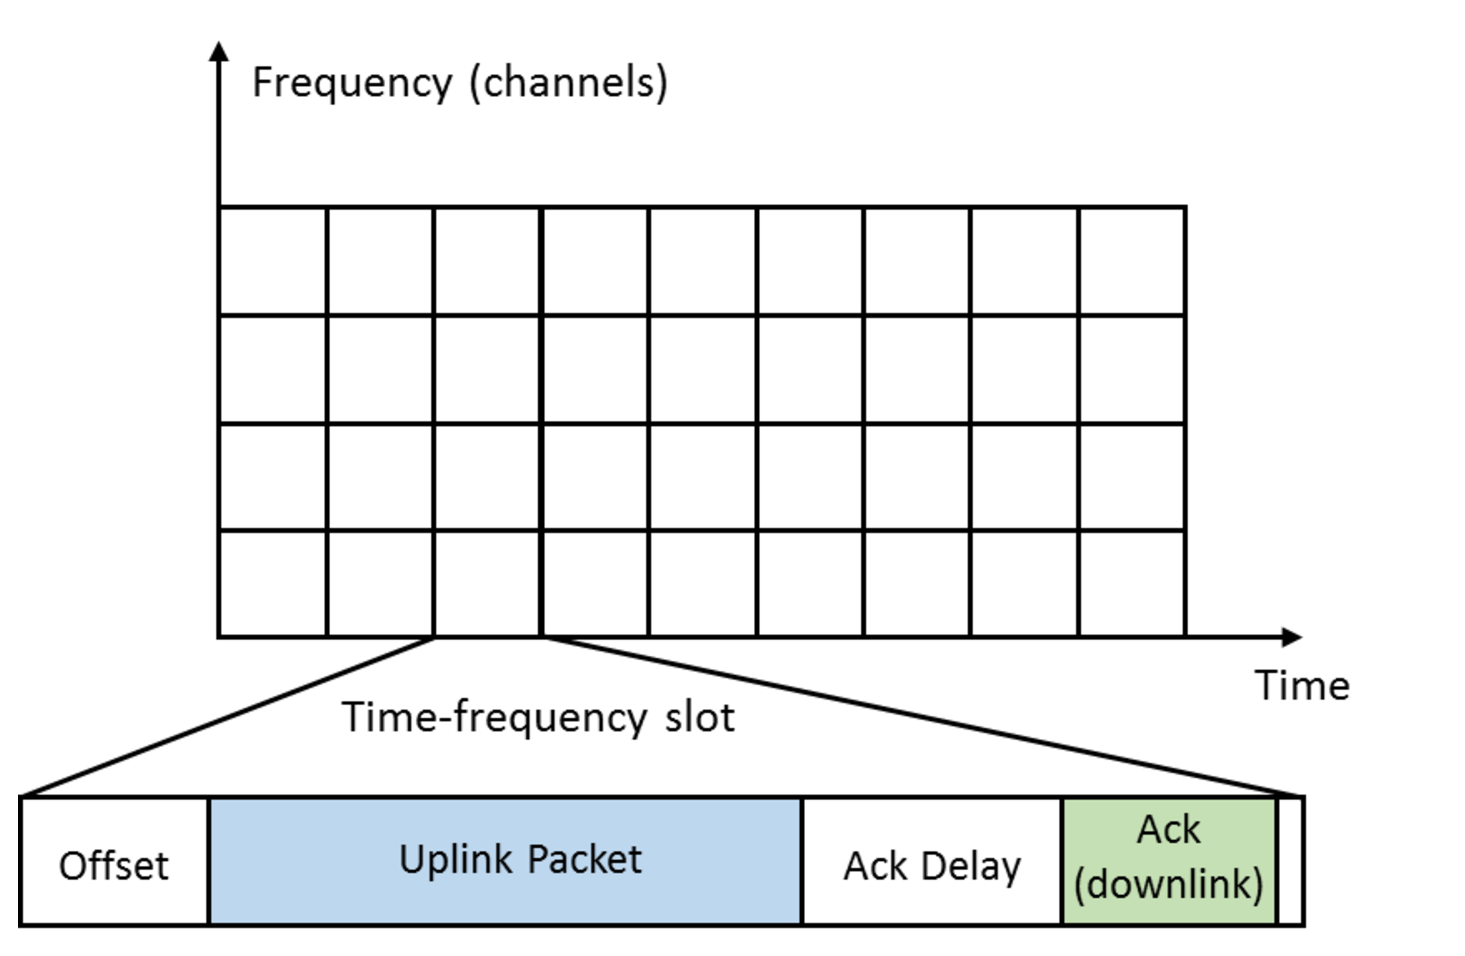
\includegraphics[scale=0.40]{protocol.eps}
    \caption[The considered time-frequency slotted protocol. Each frame is composed by a fixed duration uplink slot in which the end-devices transmit their (uplink) packets. If a packet is well received, the gateway replies by transmitting an \Ack, after the ack delay.]{The considered time-frequency slotted protocol. Each frame is composed by a fixed duration \textcolor{blue}{uplink slot} in which the end-devices transmit their \textcolor{blue}{(uplink) packets}. If a packet is well received, the gateway replies by transmitting an \textcolor{darkgreen}{\Ack}, after the ack delay.}
    \label{fig:41:protocol}
\end{figure}


\textbf{Static vs dynamic devices.}
%
We make the following assumptions on the network.
We assume that there are two types of end-devices in the network:
\begin{itemize}
    \item
    \emph{Static} end-devices are identical, and each of them uses only \emph{one} channel to communicate with the gateway, with no loss of generality.
    %  if devices random access the channels.
    Their choice is assumed to be fixed in time (\ie, stationary). The traffic generated by these devices is considered as an interfering traffic for other devices.
    \item
    \emph{Dynamic} (or \emph{smart}) end-devices can use all the available channels, by quickly changing their communication channel at any time slot, following a Machine Learning policy.
    For that end, they use their history of past communication successes or failures they experienced in each channel, to learn about channel availability.
    We also assume that the dynamic end-devices can run simple embedded decision making algorithms, and have limited but reasonable computing as well as storage capacities.
    Note that of course we assume a limited storage capacity, so no device stores the full history of communication successes and failures, but they only store average rates (which can be stored using one float number for each of the $K$ channels).
    Our goal is to propose a learning algorithm than can be implemented by each dynamic device, in a decentralized and independent manner, in order to improve their successful communication rate automatically.
\end{itemize}

We further assume that there are $K \geq 2$ channels, $D \geq 0$ dynamic end-devices, and $S \geq 0$ static devices
with $0 \leq S_k \leq S$ static devices in channel $k \in [K]$ (so $S = \sum_{k=1}^{K} S_k$).


\textbf{Random emission patterns:}
%
We suppose that all devices follow the same emission pattern, being fixed in time, and we choose to model it as a simple Bernoulli process:
all devices have the same probability to send a packet in any (discrete) temporal slot, and we denote $p \in (0, 1)$ this probability\footnote{~In the experiments below, $p$ is about $10^{-3}$, because in a crowded network $p$ should be smaller than $K / (S + D)$ for all devices to communicate successfully (in average).}.
The parameter $p$ essentially controls the frequency of communication for each device, once the time scale is fixed, and $1/p$ is proportional to the \emph{duty cycle}.
% (\ie, real time during two messages)
For instance, for IoT devices sending messages with a duration of $1$ second and possibly at every second, then on a daily basis we have $p = 1 / (12 \times 60 \times 60) \simeq 1.5 \times 10^{-5}$.


\textbf{Some assumptions on the network occupation:}
%
We focus on \emph{dense networks}, in which the number of devices $S + D$ is very large compared to $K$ (for instance, about $1000$ to $100000$, while $K$ is about $4$ to $256$).
As this problem is only interesting if devices are able to communicate reasonably efficiently with the gateway, we assume that devices only communicate occasionally, \ie, with a low \emph{duty cycle}, as it is always considered for IoT.
Note that even unlicensed bands have such limitations, as for instance this is a strict requirement for any device using the \SI{868}{\mega\hertz} ISM band in Europe (and its regulation also enforces a maximum transmission power, but we do not consider power transmission in this work).
%
We prefer this choice rather than non-crowded networks, \ie, where $S + D \leq K$, as the former makes more sense for realistic IoT networks.\\
% \footnote{~Here, $K$ will typically be about $10$ different radio channels, usually in the same RF band and with separate mean carrier frequencies, and the number of devices will be of the order of $1000$ to $10000$.}.
\indent
On the opposite, imagine if there were only $K=4$ channels being occupied by $D+S = 100$ devices, each communicating with a high rate of $p=1/10$, with a non-zero occupancy in each channel (\ie, $\forall k, S_k > 0$). Then, almost all time slots will lead to collisions in all channels, for a uniformly random access scheme, and thus the network efficiency (\ie, successful communication rate) will be so close to zero that using learning algorithms cannot improve much.
Such scenario is not our target of interest, and thus we prefer to only consider feasible scenarios where $p$ is smaller than $K/(S+D)$, in order to \emph{have an average of active devices not larger\footnote{~In Chapter~\ref{chapter:5} we simply consider the case of $p=1$ and $M = D \leq K$ dynamic devices, referred to as \emph{players}.} than the number of channels}.


\textbf{Link with the MAB model:}
%
All devices follow a Bernoulli emission process.
Consider the network from the point of view of one dynamic device:
every time a dynamic device has to communicate with the gateway,
it has to choose one channel (at each transmission $t \geq 1, t \in \mathbb{N}$), denoted as $A(t) = k \in[K]$.
Then, the dynamic device waits in this channel $A(t)$ for an acknowledgement sent by the gateway, during a certain period (\eg, $5$ seconds for the example considered above).
Before sending another message (\ie, at time $t+1$), the dynamic device knows if it received or not this \Ack{} message.
%
For this reason, selecting channel (or arm) $k$ at time $t$ yields a (random) feedback, called a (binary) \emph{reward}, $r(t) \eqdef Y_{k,t} \in \{0,1\}$, being $0$ if no \Ack{} was received before the next message, or $1$ if \Ack{} was successfully received.
The goal of the dynamic device is to minimize its packet loss ratio, or equivalently, to maximize its number of successful transmissions, or its cumulative reward,
$\sum_{t = 1}^T r(t),$
which is the usual objective in MAB problems (see Section~\ref{sec:2:notations}).


This problem is a special case of the stochastic MAB with
% , where the sequence of rewards drawn from a given arm $k$ is assumed to be  \emph{i.i.d.}, under some distribution $\nu_k$, that has a mean $\mu_k$.
% Several types of reward distributions have been considered in the literature, and rewards are binary in our model.
% We consider only
Bernoulli distributions.
% , in which $r_k(t) \sim \mathrm{Bern}(\mu_k)$, that is, $r_k(t) \in \{0,1\}$ and $\mathbb{P}(r_k(t) = 1) = \mu_k \in [0,1]$.
Contrarily to many previous work done in the CR field (\eg, Opportunistic Spectrum Access) \cite{Jouini10,Jouini12},
the reward $r(t)$ does \emph{not} come from a sensing phase before sending the $t$-th message, as it would do for any ``listen-before-talk'' model.
In our model, rewards rather come from receiving or not an acknowledgement from the gateway, between the $t$-th and $t+1$-th messages. A reward of one indicates that the acknowledgement was received on time, and a reward of zero indicates the opposite.

The problem parameters
% are $\mu_1,\dots,\mu_K$, the mean availability of the channels,
are $S_1, \dots, S_K$ which represent the (stationary) occupancy of the channels by the static devices,
and they are unknown to each dynamic device, so to maximize their cumulated rewards, they must learn the distributions of the channels, in order to be able to progressively improve their respective successful communication rate.
%
The goal is thus to propose a simple sequential algorithm to be applied identically and independently by each dynamic device, in a fully distributed setting (each device runs its own algorithm, from its observations), in order to minimize collisions and maximize the fraction of successful transmissions of all the dynamic devices.
%
This requires to tackle the so-called \emph{exploration-exploitation dilemma}: a device has to try all channels a sufficient number of times to get a robust estimate of their qualities, while not selecting the worst channels too many times.
%
Before presenting the MAB algorithms used in the experiments, we present some simple baseline (reference) policies.


% ------------------------------------------------------------------------
\subsection{Three reference policies}\label{sub:41:threeReferencePolicies}

We present three different policies that can be used to assess the efficiency of the learning algorithms presented later on.
The first one is naive but can be used in practice, while the two others are very efficient but require full knowledge on the system (\ie, an oracle) and are thus unpractical.
%
They are however useful for our numerical simulations, and are used as references, to show that our MAB-based approaches quickly learn to perform almost optimally.
%
Their short names are used in the legend on Figures~\ref{fig:41:from10to100}, \ref{fig:41:figure4appendix}), and are given in ``quotes'' in the corresponding paragraphs.


\paragraph{$1^{\text{st}}$ - Naive policy: Random Channel Selection} (``\textcolor{darkgreen}{Random}'')

We derive here the probability of having a successful transmission, for a dynamic device, in the case where all the dynamic devices make a purely random channel selection (\ie, uniform on $i \in [K]$).
This reflects a naive policy that could be implemented by all the dynamic devices, and it provides a reference scenario to compare against.
Note that even nowadays this is still the solution implemented for real IoT devices deployed in new LoRaWAN networks.

In this case, for one dynamic device, a successful transmission happens if it is the only device to choose channel $k$, at that time slot.
the $S_k$ static devices in each channel $k$ are assumed to be independent, and static and dynamic devices are assumed to \emph{not} transmit at each time $t$ with a fixed probability $1-p$,
so probability of successful transmission is computed as follows

\begin{equation}
    \Pr(\text{success}|\text{sent}) = \sum_{k=1}^{K} \underbrace{\Pr(\text{success}|\text{sent in channel}\;k)}_{\text{No one else sent in channel}\; k} \; \underbrace{\Pr(\text{sent in channel}\,k)}_{= 1/K, \text{ by uniform choice}}
\end{equation}

All dynamic devices follow the same policy in this case, so the probability of transmitting at that time in channel $k$ for any dynamic device is $p / K$, and there are $D-1$ other dynamic devices.
As they are independent, the probability that no other dynamic device sent in $i$
% $\Pr(\text{no other dynamic device sent in}\;i)$,
is $q = \Pr(\bigcap_{k=1}^{D-1} \text{device}\;k\;\text{did not sent in}\;i) = \prod_{k=1}^{D-1} \Pr(\text{device}\;k\;\text{did not sent in}\;i)$. And $\Pr(\text{device}\;k\;\text{sent in}\;i) = p \times 1 / K$, by uniform choice on channels and the Bernoulli emission hypothesis. So $q = \prod_{k=1}^{D-1} (1 - p/K) = (1-p/K)^{D-1}$. Thus we can conclude,
%
\begin{align}\label{eq:41:strategynaive}
    \Pr(\text{success}|\text{sent})
    & = \sum_{k=1}^{K} \underbrace{(1 - p / K)^{D-1}}_{\text{No other dynamic device}} \times \underbrace{(1-p)^{S_k}}_{\text{No static device}} \times\; \frac{1}{K} \nonumber \\
    & = \frac{1}{K} \left(1-\frac{p}{K}\right)^{D-1} \sum_{k=1}^{K} (1-p)^{S_k} .
\end{align}
%
This expression \eqref{eq:41:strategynaive} is constant (in time), and easy to compute numerically, but comparing the successful transmission rate of any policy against this naive policy is important, as any efficient learning algorithm should outperform it
(maybe after a long enough initial learning period).


\paragraph{$2^{\text{nd}}$ - (Unachievable) Optimal oracle policy} (``\textcolor{orange}{Optimal}'')

We investigate here the optimal policy that can be achieved if the dynamic devices have a perfect knowledge of the repartition of static devices $(S_k)_k$, and a fully centralized decision making\footnote{~This optimal policy needs an \emph{oracle} seeing the entire system, and affecting all the dynamic devices, once and for all, for a fixed stationary scenario, in order to avoid any signaling overhead. This is not possible in IoT contexts as several completely independent networks may operate in a single place.} is possible.
We want to find the stationary repartition of devices into channels that maximizes the probability of having a successful transmission.

If the oracle chooses a fixed configuration of dynamic devices, it means that for each dynamic device the oracle affects it to a unique channel for all time steps.
Then there is a number $D_k$ of devices affected to channel $k$ being fixed in time (\ie, stationary),
and thus this probability is computed as before:
%
\begin{align}\label{eq:41:prob_col}
    \Pr(\text{success}|\text{sent})
    & = \sum_{k=1}^{K} \Pr(\text{success}|\text{sent in channel}\;k) \; \Pr(\text{sent in channel}\;k) \nonumber \\
    & = \sum_{k=1}^{K} \underbrace{(1 - p)^{D_k - 1}}_{\;\;D_k - 1 \;\text{others}\;\;} \times \underbrace{(1 - p)^{S_k}}_{\;\;\text{No static device}\;\;} \times \underbrace{ D_k / D }_{\;\;\text{Sent in channel}\; k\;\;}.
\end{align}

Consequently, an optimal allocation vector $(D_1,\dots,D_{K})$ is a solution of the following real-valued constraint optimization problem:
%
\begin{subequations}\label{eq:41:prob}
\begin{align}
    % \begin{cases}
    \underset{D_1,\dots,D_{K}}{\arg\max}\; & \sum_{k=1}^{K} D_k (1 - p)^{S_k + D_k -1}, \label{eq:41:optPb}\\
    \text{such that}\;\; & \sum_{k=1}^{K} D_k = D, \label{eq:41:eqCstr}\\
    & D_k \geq 0 \qquad \forall k\in\llbracket 1;K\rrbracket . \label{eq:41:ineqCstr}
    % \end{cases}
\end{align}
\end{subequations}

\begin{proposition}\label{prop:41:Lagrangian}
\begin{leftbar}[propositionbar]  % XXX leftbar propositionbar, comment if needed
    The \emph{Lagrange multipliers} method \cite{BoydVanderberghe04} can be used to solve the constraint real-valued maximization problem introduced in equation \eqref{eq:41:prob}.
    %
    It gives a closed form expression for the (unique) optimal solution $D_k^*(\lambda)$, depending on the system parameters, and the unknown Lagrange multiplier $\lambda \in \mathbb{R}$.
    %
    \begin{equation}\label{eq:41:Dilambda}
        D_k^*(\lambda) = \left(\frac{1}{\log(1-p)}\left[ \mathcal{W}\left(\frac{\lambda \e}{(1-p)^{S_k-1}} \right)-1 \right]\right)^{+} .
    \end{equation}
\end{leftbar}  % XXX leftbar propositionbar, comment if needed
\end{proposition}
%
\begin{smallproof}
\begin{itemize}
    \item
    In a realistic scenario, we can assume that $D_k\leq \frac{-2}{\ln\left(1-p\right)} \approx \frac{2}{p},\quad \forall k\in\llbracket 1;K \rrbracket$. For such values for $D_k$, the objective function $f: (D_1, \dots, D_{K}) \mapsto \sum_{k=1}^{K} D_k (1 - p)^{S_k + D_k -1}$ is concave as the sum of concave functions
    \footnote{~It is worth noting that $f$ is neither concave nor quasi-concave on $[0,\infty)^{K}$ \cite{Luenberger68,Yaari77}.}.
    \item
    The Lagrange multipliers method can be applied to the optimization problem \eqref{eq:41:optPb}, with a concave objective function $f$, linear equality constraints \eqref{eq:41:eqCstr} and linear inequality constraints \eqref{eq:41:ineqCstr}. The strong duality condition is satisfied in this case \cite{BoydVanderberghe04}, so finding the saddle points will be enough to find the maximizers.
    % \item
    % \hfill{}$\square$
    \end{itemize}
    More details are given in Section~\ref{sec:4:proofLagrangian} in the Appendix of this Chapter.
\end{smallproof}

Where in the equation~\eqref{eq:41:Dilambda}, $(a)^{+} \eqdef \max(a,0)$, and $\mathcal{W}$ denotes the $\mathcal{W}$-Lambert function which is the reciprocal bijection of $x \mapsto x e^x$ on $\mathbb{R^+} = [0, +\infty)$ (which can be computed numerically in an efficient manner, \cite{Corless96}).
Moreover, condition \eqref{eq:41:eqCstr} implies that the Lagrange multiplier $\lambda$ is the solution of the constraint $\sum_{k=1}^{K} D_k^*(\lambda) = D$.
%
This single constraint can be solved numerically, with simple one-dimensional root finding algorithms.
Solving the optimization problem provides the optimal real number value for $D_k^*$, which has to be rounded\footnote{~Any rounding choice will give about the same repartition, up-to a difference of only one device by channel, and so we chose to round from below for the first channels.} to find the optimal number of devices for channel $k$:
%
$\widehat{D_k} = \lfloor D_k^* \rfloor$ for $1 \leq k < K$, and $\widehat{D_{K}} = D - \sum_{k=1}^{K - 1} \widehat{D_k}$.


\paragraph{$3^{\text{rd}}$ - A greedy approach of the oracle strategy} (``\textcolor{deeppurple}{Good sub-optimal}'')

We propose a \emph{sequential} approximation of the optimal policy:
the third solution is a sub-optimal naive policy, simple to set up, but also unpractical as it also needs an oracle.
End-devices are iteratively inserted in the channels with the lowest load (\ie, the index $k$ minimizing $S_k + D_k(\tau)$ at global time step $\tau$). Once the number of devices in each channel is computed, the probability of sending successfully a message is also given by equation \eqref{eq:41:prob_col}.
This is the policy that would be used by dynamic devices if they were inserted one after the other, and if they had a perfect knowledge of the channel loads.


% ----------------------------------------------------------------------
\subsection{Sequential policies based on bandit algorithms}
\label{sub:41:sequentialPolicies}
% ----------------------------------------------------------------------

While the stochastic MAB model has been used to describe some aspects of Cognitive Radio systems, it is in principle not suitable for our IoT model, due to the non-stationarity of the channels occupancy, caused partly by the learning policy used by dynamic devices, but mainly by their random activation processes.
%
In our model, every dynamic device implements its own learning algorithm, \emph{independently}.
For one device, the time $t$ refers to the number of time it accessed the network (following its Bernoulli transmission process, \ie, its duty cycle), \emph{not} the total number of time slots from the beginning, as rewards are only obtained after a transmission, and IoT devices only transmit sporadically, due to low transmission duty cycles.


\textbf{Using a bandit algorithm for IoT devices:}
%
Our IoT application is challenging in that there are \emph{multiple} players (the dynamic devices) interacting with the \emph{same} arms (the channels), without any centralized communication (they do not even know the total number of dynamic devices).
%
% Considered alone, each dynamic device
We propose algorithms in which each dynamic device ignores all the other one and
implements a learning algorithm to play a bandit game.
%
In each time slot, if it has to communicate (which happens with probability $p$), then it chooses a channel and it receives a reward $1$ if the transmission is successful, $0$ otherwise.
Each device aims at maximizing the sum of the rewards collected during its communication instants, which shall indeed maximize the fraction of successful transmissions. Besides the modified time scale (rewards are no longer collected at every time step), this looks like a usual bandit problem.
However, it cannot be modeled as a stochastic MAB, as the rewards are (unfortunately) \emph{not} \iid: they not only depend on the (stationary, \iid) behavior of the static devices, but also on the behavior of other dynamic devices, that is not stationary (because of learning and random activation of each device).
%
Despite this, we show in the next subsection that running a stochastic bandit algorithm for each device based on its own rewards is surprisingly successful.


\textbf{Considered algorithms.}
%
% In our model, every dynamic device implements its own algorithm, \emph{independently}.
% For one dynamic device, the time $t$ is the total number of sent messages from the beginning, as rewards are only obtained after a transmission.
%
The two algorithms we consider are \UCB{} (``\textcolor{blue}{UCB}'' in the figures)
and Thompson sampling (TS) (``\textcolor{red}{Thompson-sampling}''),
and they are presented in Section~\ref{sec:2:famousMABalgorithms}.
% originally $\alpha$ was set to $2$ \cite{Auer02}, but empirically $\alpha = 1/2$ is known to work better (uniformly across problems), and $\alpha > 1/2$ is advised by the theory \cite{Bubeck12}.
%
The \UCB{} algorithm uses $\alpha = 1/2$ in our experiments.
The TS algorithm is known to be empirically efficient, and for these reasons it has been used successfully in various applications, including problems from Cognitive Radio \cite{Toldov16,Mitton16}, and also in previous work on decentralized IoT-like networks \cite{Darak16}.
% although being simple and easy to implement, is known to perform well for stochastic problems, for which it was proven to be asymptotically optimal \cite{AgrawalGoyal11,Kaufmann12Thompson}.


\textbf{\emph{Adversarial} bandit algorithms?}
%
Instead of using MAB algorithms assuming a stochastic hypothesis on the system, we could try to use MAB algorithms designed to tackle a more general problem, that makes no hypothesis on the interfering traffic.
The \emph{adversarial MAB} algorithms is a broader family, of which a well-known and efficient example is the $\mathrm{Exp}3$ algorithm \cite{Auer02,Bubeck12}.
Empirically, the $\mathrm{Exp}3$ algorithm turned out to perform significantly worse than both \UCB{} and TS in the same experiments,
therefore we did not report results here.
% % FIXME maybe we should... ?
% %(see Section \ref{sub:41:numericalResults}).
% However, contrarily to the two stochastic algorithms, the use of $\mathrm{Exp}3$ is correctly justified, even in the non-stationary model, as its performance guarantees are true in \emph{any} setting.
% But it is not so surprising that it performs worse, as the theoretical performance guarantees of adversarial MAB algorithms are an order of magnitude
% %\footnote{~We preferred not to talk about \emph{regret} in this study, but in a few words: it is a measure of how \emph{bad} the algorithm performed in terms of its accumulated rewards, in comparison to the best possible policy, and should be as small as possible. For stochastic algorithms, being ``efficient'' means having a regret bounded as $R_T = \mathcal{O}(\log T)$, but for adversarial algorithms, it means having $R_T = \mathcal{O}(\sqrt{K T})$.}
% worse than the one for stochastic ones.
% (in their respective case of application).
% Further research on this aspect could lead to interesting future works.



% ------------------------------------------------------------------------
\subsection{Numerical results}\label{sub:41:numericalResults}

% Simulation parameters
We suppose a network with $S + D = 2000$ end-devices, and one IoT gateway.
Each device sends packets following a Bernoulli process, of probability $p = 10^{-3}$ (\eg, this is realistic: one packet sent about every $20$ minutes, for time slots of $1\mathrm{s}$).
The RF band is divided in $K = 10$ channels.
Each static device only uses one channel, and their uneven repartition in the $10$ channels is chosen as $(S_1,\cdots, S_{K}) = S \times (0.3, \, 0.2, \, 0.1, \, 0.1, \, 0.05, \, 0.05, \, 0.02, \, 0.08, \, 0.01,$ $0.09)$, to keep the same proportions when $S$ decreases. The dynamic devices have access to all the channels, and use learning algorithms.
%to find the least loaded.
%
We simulate the network during $10^6$ discrete time slots, during which each device transmits on average $1000$ packets (\ie, the learning time is about $1000$ steps, for each algorithm).
We tried similar experiments with other values for $K$ and this repartition vector, and results were similar for non-homogeneous repartitions.

Clearly, the problem is less interesting for a homogeneous repartition, as all channels appear the same for dynamic devices, and so even with $D$ small in comparison to $S$, the system behaves like in Figure~\ref{fig:41:100intelligent}, where the performance of the five approaches are very close.

\begin{figure}[!h]
    \centering
    \subfloat[][10\% of dynamic devices]{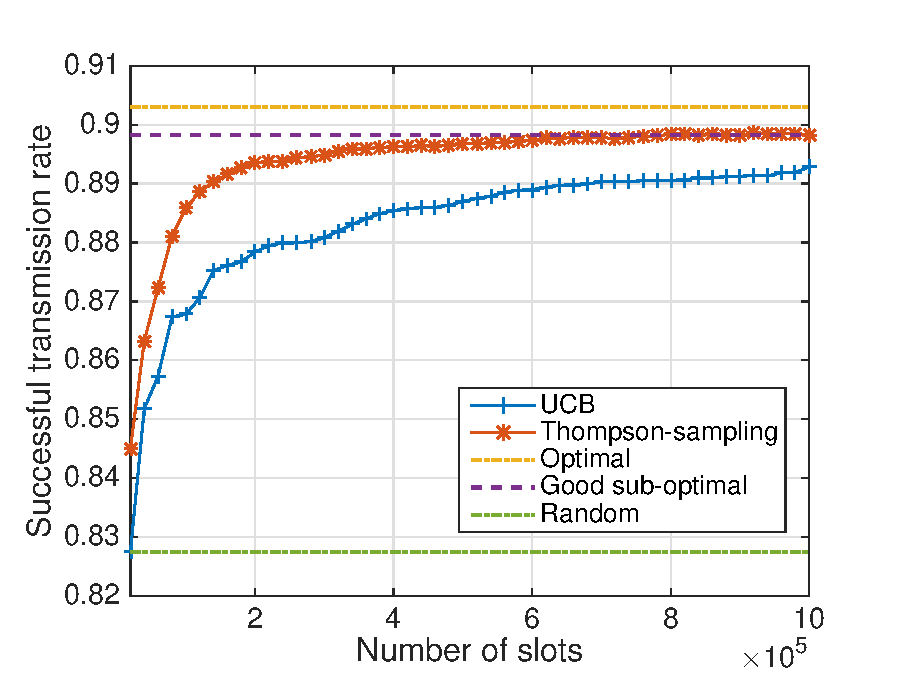
\includegraphics[width=0.52\textwidth]{10intelligent.eps}
    \label{fig:41:10intelligent}}
    %
    \subfloat[][30\% of dynamic devices]{\includegraphics[width=0.52\textwidth]{30intelligent.eps}
    \label{fig:41:30intelligent}}
    %
    \vspace*{-10pt}
    \subfloat[][50\% of dynamic devices]{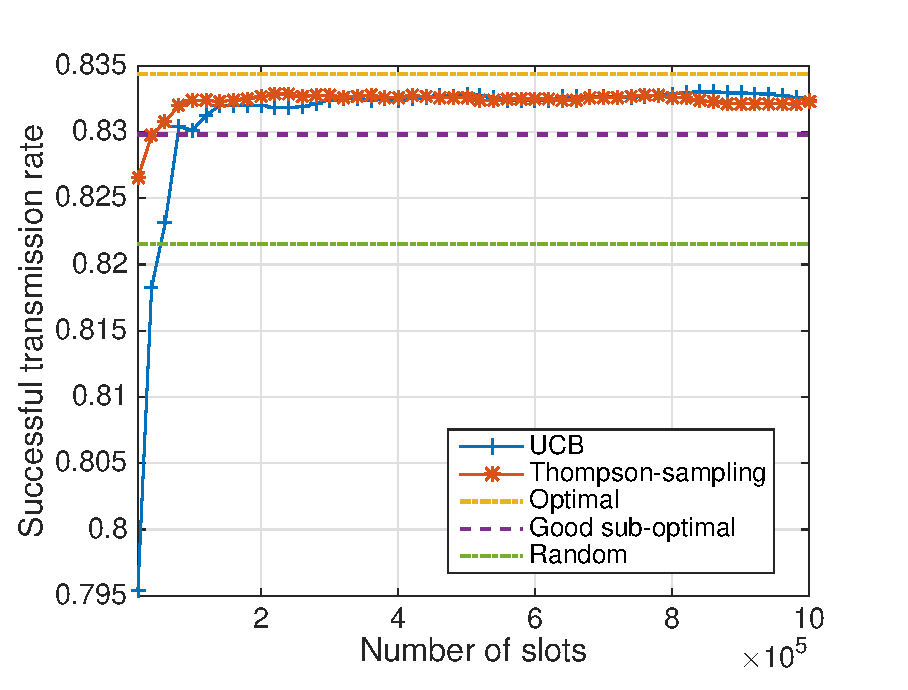
\includegraphics[width=0.52\textwidth]{50intelligent.eps}
    \label{fig:41:50intelligent}}
    %
    \subfloat[][100\% of dynamic devices]{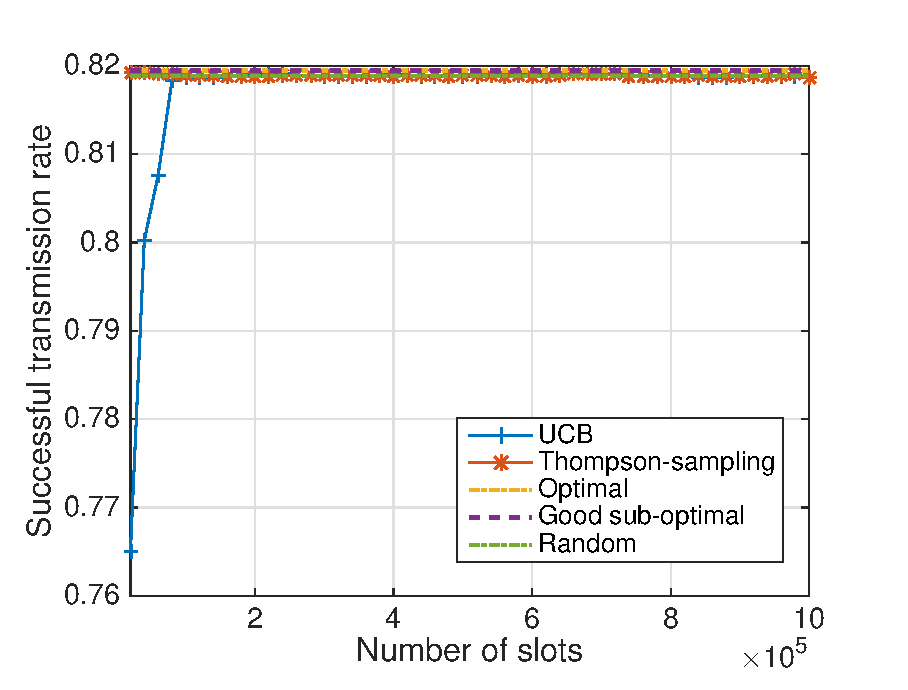
\includegraphics[width=0.52\textwidth]{100intelligent.eps}
    \label{fig:41:100intelligent}}
    \caption{Performance of two MAB algorithms (\UCB{} and Thompson Sampling), compared to extreme reference policies without learning or oracle knowledge, when the proportion of dynamic end-devices in the network increases, from $10\%$ to $100\%$.}
    \label{fig:41:from10to100}
    \vspace*{-10pt}
\end{figure}


\paragraph{First results.}
%
Figure~\ref{fig:41:from10to100} presents the successful transmission rate as a function of time.
The two MAB algorithms, \UCB{} and Thompson Sampling (TS), are compared against the naive random policy (which are outperformed easily by the MAB algorithms), and the two (optimal and greedy) oracle policies (which outperform slightly the MAB algorithms).
The results are displayed when $10\%$, $30\%$, $50\%$ and $100\%$ of the traffic is generated by dynamic devices.


We can see in Figure~\ref{fig:41:from10to100} that the TS algorithm (\textcolor{red}{in red}) outperforms the \UCB{} algorithm (\textcolor{blue}{in blue}), when the number of end-devices is below 50\%. When the number of end-devices is higher, both algorithms have almost the same performance, and perform well after a small number of transmissions (\ie, they show quick convergence).
Moreover, we can see in Figures~\ref{fig:41:10intelligent}, \ref{fig:41:30intelligent}, and \ref{fig:41:50intelligent} that both have better success rate than the random policy and the probability of successful transmission is between the optimal oracle and suboptimal oracle policies.
For instance, for $10\%$ of dynamic devices, after about $1000$ transmissions, using \UCB{} over the naive uniform policy improved the successful transmission rate from $83\%$ to $88\%$, and using Thompson Sampling improved it to $89\%$.
Increasing the number of end-devices decreases the gap between the optimal and random policies:
as expected intuitively, the more dynamic devices, the less useful are learning algorithms, and basically for networks with only dynamic devices, the random policy is as efficient as the optimal one, as seen in Figures~\ref{fig:41:100intelligent} and on the right end side of Figure~\ref{fig:41:perf_learning}.

\begin{figure}[!h]
    \centering
    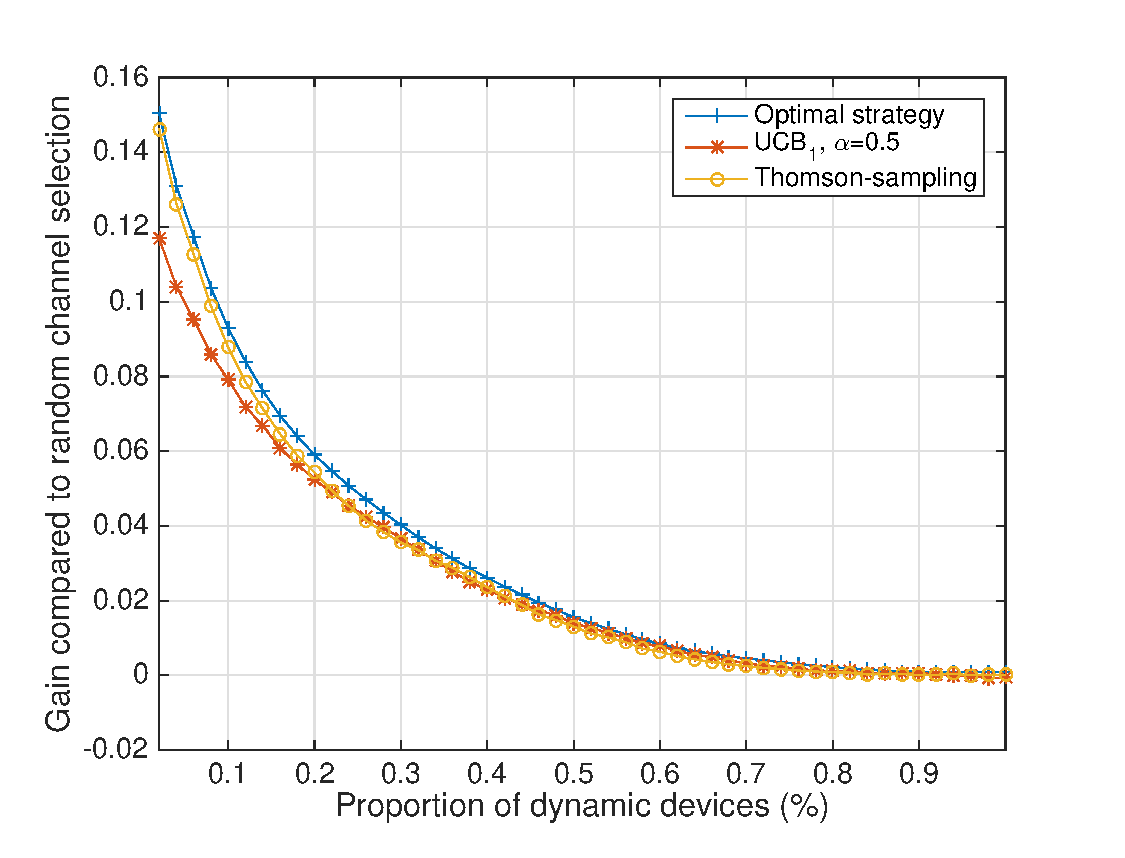
\includegraphics[scale=0.65]{perf_learning.eps}
    \caption{Learning with \UCB{} and Thomson Sampling, with many dynamic devices.
        The learning gain, for each device, decreases with the proportion of dynamic devices in the network.
        Note that the values ($16\%$ etc) depend on the repartition of static devices into the $K$ channels (\ie, $S_1,\dots,S_K$) but the general profile of this plot does \emph{not} depend much on these parameters.
        % Both algorithms achieve close to optimal performance after a reasonable learning time.
    }
    \label{fig:41:perf_learning}
\end{figure}


\textbf{Successful transmissions rate as a function of the number of dynamic devices.}
%
To better assess the evolution of the optimal policy compared to the random one, we have displayed on Figure~\ref{fig:41:perf_learning} the evolution of the gain, in terms of successful transmissions rate, provided by the optimal oracle and the two learning policies, after $10^6$ time slots, \ie, about $1000$ transmissions for each IoT device.
We can see that when the proportion of end-devices is low (\eg, $1\%$ of devices are dynamic), the optimal policy provides an improvement of $16\%$ compared to random channel selection.
The TS algorithm always provides near-optimal performance, but the \UCB{} algorithm has a lowest rate of convergence and performs consequently worse after $1000$ transmissions, for instance it only provides a gain of $12\%$ for the same proportion of dynamic devices ($1\%$),
for the considered values of $S_1,\dots,S_K$.

\begin{figure}[!h]
    \centering
    \subfloat[][10\% of intelligent devices]{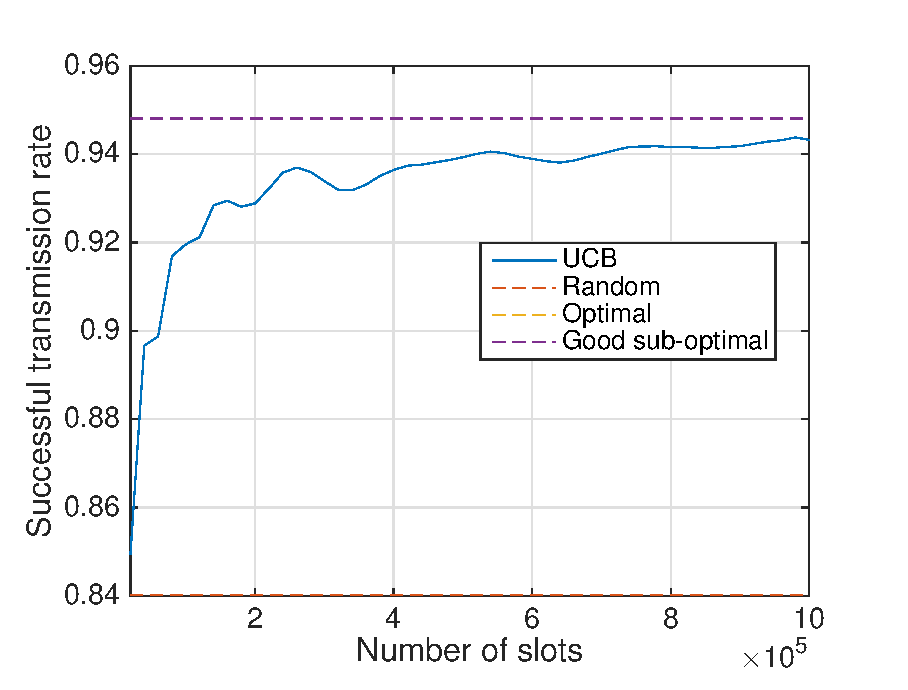
\includegraphics[width=0.47\textwidth]{ch2_10.eps}
    \label{fig:41:ch2_10}}
    %
    \subfloat[][30\% of intelligent devices]{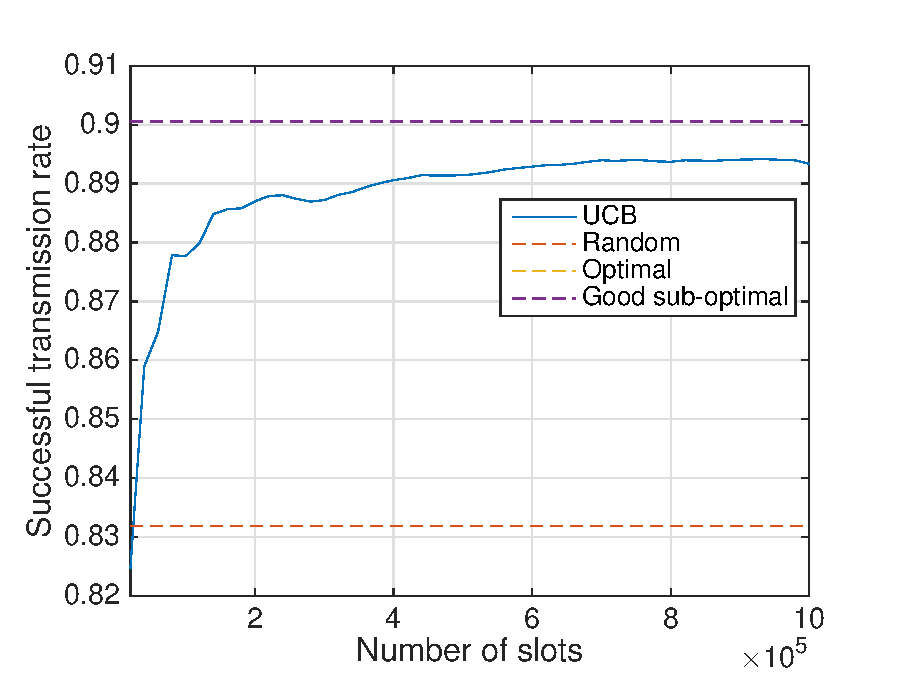
\includegraphics[width=0.47\textwidth]{ch2_30.eps}
    \label{fig:41:ch2_30}}
    %
    \vspace*{-10pt}
    \subfloat[][50\% of intelligent devices]{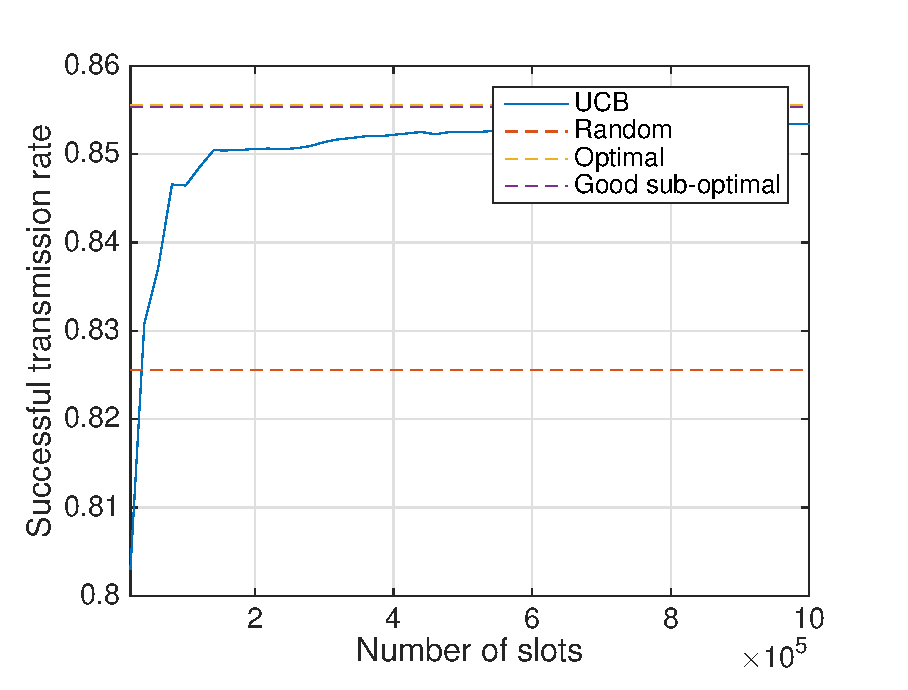
\includegraphics[width=0.47\textwidth]{ch2_50.eps}
    \label{fig:41:ch2_50}}
    %
    \subfloat[][100\% of intelligent devices]{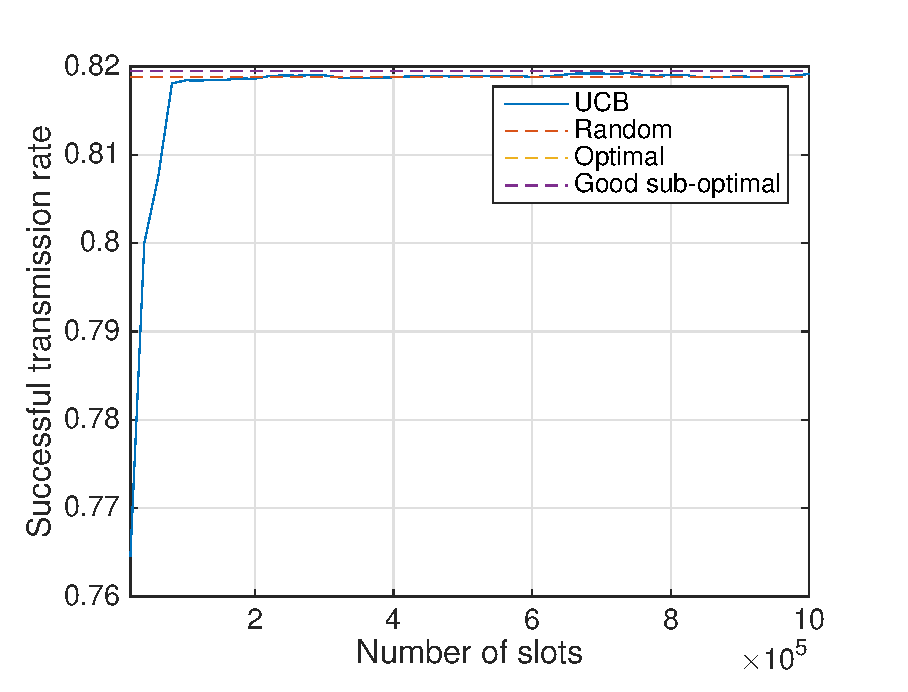
\includegraphics[width=0.47\textwidth]{ch2_100.eps}
    \label{fig:41:ch2_100}}
    \caption{Performance of the UCB bandit algorithm for the special case of uniform repartition of the static devices, when the proportion of intelligent devices in the network increases, from $10\%$ to $100\%$.}
    \label{fig:41:figure4appendix}
\end{figure}

Figure~\ref{fig:41:perf_learning} also shows that learning keeps near-optimal performance even when the proportion of devices becomes large.
Note that when this proportion increases, the assumptions of a stochastic MAB model are clearly violated, and there is no mathematical justification for the efficiency of TS and \UCB{} algorithms.
Hence, it is surprising to have near optimal performance with stochastic MAB algorithms applied to partly or fully dynamic scenarios.


\textbf{A safety check.}
%
We include another simulation in Figure~\ref{fig:41:figure4appendix}, with a uniform repartition of static devices (\ie, $\forall k, S_k = S/K$), to check that learning approach (here, only \UCB)
also gives interesting gain of performance, and achieve a close-to optimal successful transmission rate.
Except for the limit case of $100\%$ of dynamic devices, which corresponds to Figures~\ref{fig:41:100intelligent} and \ref{fig:41:ch2_100}, where the uniform access performs as well as the optimal oracle solution, the MAB-based approach almost instantly outperforms the baseline.



% \paragraph{Note on the simulation code.}
\textbf{Reproducibility.}
%
The simulation code used for the experiments in Section~\ref{sub:41:numericalResults} is for MATLAB or GNU Octave,
and it was written in collaboration with Rémi Bonnefoi, in May $2017$.
Instructions to reproduce our experiments are given, and
the code is open-sourced under the MIT License, at
\href{https://Bitbucket.org/scee_ietr/rl_slotted_iot_networks}{\texttt{Bitbucket.org/scee\_ietr/rl\_slotted\_iot\_networks}}.



\newpage  % WARNING ?
% ----------------------------------------------------------------------------
\section{Test-bed implementation of our model for real-world validation}
\label{sec:4:gnuradio}
% ----------------------------------------------------------------------

% - ``MALIN: Multi-Arm bandit Learning for Iot Networks with GRC: A TestBed Implementation and Demonstration that Learning Helps'', demo at ICT, and the companion paper ``GNU Radio Implementation of MALIN: "Multi-Armed bandits Learning for Internet-of-things Network"'', see https://hal.inria.fr/hal-02006825

\definecolor{darkblue}{rgb}{0.00,0.00,0.65}       % rgb(0,0,126)
\definecolor{darkgreen}{RGB}{0,100,0}  % rgb(0,100,0)
\definecolor{darkred}{RGB}{174,0,0}        % rgb(174,0,0)

% - ``MALIN: Multi-Arm bandit Learning for Iot Networks with GRC: A TestBed Implementation and Demonstration that Learning Helps'', demo at ICT, and the companion paper ``GNU Radio Implementation of MALIN: "Multi-Armed bandits Learning for Internet-of-things Network"'', see https://hal.inria.fr/hal-02006825

\graphicspath{{2-Chapters/4-Chapter/IEEE_WCNC_2019__DemoICT.git/pictures/}}

In this section, we present a demonstration showcased at the International Conference on Telecommunication (ICT) in June $2018$ \cite{Besson2018ICT,Besson2019WCNC}, implementing a proof-of-concept (PoC) of the model introduced in Section~\ref{sec:4:firstModel}.
%
As far as we know, this is the first demonstration of running learning algorithms on the end-device side for Internet of Things networks, in real radio conditions, as highlighted it in our paper \cite{MoyBesson2019}.

This PoC implements an IoT network the following way: one base station, one or several intelligent (\emph{i.e.}, learning) devices, embedding the proposed solution,
and a traffic generator that emulates radio interference from many other devices.
Intelligent devices communicate with the base station with a wireless ALOHA-based protocol with acknowledgements, which does not require any specific overhead for the learning.
%
Similarly to the previous section, network access is modelled as a discrete sequential decision making problem, and using the framework and algorithms from MAB learning, we show that intelligent devices can improve their access rate to the network, by using low complexity and decentralized algorithms, such as \UCB{} and Thompson Sampling.
%
This solution could be added in a straightforward and costless manner in most IoT networks, such as LoRaWAN networks, just by adding this feature at the higher level of the MAC layer, in all or only some of the devices, without any modification on the network side, and no signalling overhead for the devices.

\paragraph{Related works.}
%
This work is new for the IoT context, but previous works have similarly implemented proof-of-concepts to show that Reinforcement Learning (RL) algorithms can be used within real-world wireless communications.
Starting from $2010$, the works of W. Jouini and C. Moy \cite{Jouini09,Jouini10,Jouini12} were among the first ones to propose to use RL for Cognitive Radio, especially MAB and the \UCB{} algorithm, and proof-of-concepts were developed with C. Robert from $2013$ \cite{RobertSDR2014,MoyWSR2014}.
Between $2015$ and $2017$, C. Moy, N. Modi and S. Darak (of our team SCEE) continued to work on this direction \cite{darak2016bayesian,Darak16,modiDemo2016,kumar2016two}.
Since $2017$, S. Darak and his team at IIIT Delhi (India) have been quite active in the research on CR using MAB, and some of their recent works are illustrated with real-world demo using USRP and the MATLAB/Simulink system
\cite{KumarYadav2018,SawantKumar2018,JoshiKumar2018}.


% ----------------------------------------------------------------------
\subsection{Context of this demonstration}
\label{sub:42:motivation}
% ----------------------------------------------------------------------

We describe the way we implemented a demo where we evaluate MAB algorithms, used in combination with a pure ALOHA-based protocol, such as the ones employed in LPWAN.
This demonstration is the first implementation which aims at assessing the potential gain of MAB learning algorithms in IoT scenarios.
%
We use a TestBed designed in 2017 by the SCEE team at the Rennes campus of CentraleSupélec \cite[Appendix~3]{Bodinier17}, containing different USRP boards \cite{USRPDocumentation}, controlled by a single laptop running the GNU Radio software \cite{GNURadioDocumentation},
and where the intelligence of each device corresponds to a learning algorithm, implemented as a GNU Radio block \cite{GNURadioCompanionDocumentation} and written in Python or \texttt{C++}.

In our demo, we consider a simple wireless network, that reproduces the model of Section~\ref{sec:4:firstModel}, consisting of one base station (\ie, radio access point), and a certain interfering background traffic, assumed to be stationary (\emph{i.i.d.}), which is generated by end-devices communicating in other networks.
Some dynamic intelligent devices (end-user or autonomous devices) try to communicate with the base station, with a low-overhead protocol. This communication can be done in different channels which are also shared by devices using other networks.
Once the base station receives a packet transmitted by a dynamic device in one channel (\ie, if no collision occurred), it transmits back to it an acknowledgement in the same channel, after a fixed-time delay, as it is done in the LoRaWAN standard.
This \emph{Ack} allows the device to learn about the channel quality (\ie, mean availability) and thus, to use learning algorithms for the purpose of best channel selection.

We can generate scenarios with different parameters (number of channels, interfering traffic load on each channel, etc) in order to evaluate the performance of learning in various settings.
Moreover, we compare the performance of learning strategies with that of the random uniform access to channels, which is the current state-of-the-art of commercial LPWAN solutions \cite{Raza17}.
%
This allows to check that in case of uniform traffic, when there is nothing to learn, the intelligent devices at least do not reduce their successful communications rate in comparison to the naive devices.
This also shows that in case of non-uniform stationary traffic, MAB learning algorithms indeed help to increase the global efficiency of the network by improving the success rate of the intelligent devices.
%
The benefits are twice and of primary importance for IoT networks:
the proposed approach can mitigate RF collisions,
and enhance intelligent device battery lifetime if they do retransmissions.

% We refer to Section~\ref{sec:2:famousMABalgorithms} which presented two bandit algorithms, \UCB{} and Thompson Sampling,
% which are both known to be efficient for stationary \emph{i.i.d.} rewards and are shown to be useful in our setting (in Section~\ref{sub:42:results}).
% Then we discuss the relevance of a MAB model for our IoT application.


% \paragraph{Outline.}

% The rest of this section is organized as follows.
% Our implementation is presented in Section~\ref{sub:42:implementation}, with details about the user interface, and results are given in Section~\ref{sub:42:results}.


% ----------------------------------------------------------------------
\subsection{Physical model and user interface of our GNU Radio implementation}
\label{sub:42:implementation}
% ----------------------------------------------------------------------

In this section, we present our implementation of MAB algorithms in the model of IoT networks presented in Section~\ref{sub:41:systemModel}.
We first describe the simplified physical layer of this demo, then we present our GNU Radio implementation.


\textbf{Physical layer and protocol.}
%
We implement a simple PHY/MAC layers solution, in order to demonstrate the possibility of improvement of the performance of IoT communications in unlicensed bands. We could have used any physical layer and any ALOHA-based protocol.
We choose to implement our own physical layer and protocol, for both clarity and conciseness, and because developing a complete IoT network protocol stack is no more my research work and would have fall outside of the scope of this thesis.

Regarding the physical layer, we consider a QPSK constellation (\emph{Quadrature Phase-Shift Keying}). Moreover, we use simplified packets composed of two parts.
The first part is the \emph{preamble} which is used for the purpose of synchronization (phase correction).
Then, we have the \emph{index} of the user, which is a sequence of QPSK symbols.
For example, this index can be a simple QPSK symbol ($\pm1\pm1j$), or a sequence of QPSK symols if the PoC has to consider more users.
With $\ell$ QPSK symbols, we can indeed fit at most $4^{\ell}/2 = 2^{2\ell-1}$ devices, and not $4^{\ell}$ due to the use of a conjugate index to send back acknowledgements from the base station.
Once the base station receives an uplink packet, it detects this index and transmits an acknowledgement which has the same frame structure, but where the index is the conjugate of the index of the uplink packet ($z \mapsto \overline{z}$, \emph{e.g.}, $1+j \mapsto 1-j$).
Thanks to this index, we can have several devices communicating with the same base station.
%
In turn, the end-device that receives the acknowledgement demodulates it, and checks if the index is the conjugate of its own index.
In this case, the \emph{Ack} was sent for him, and it knows that its packet has been received and decoded correctly by the base station.

\begin{figure}[!b]
    \centering
    
\includegraphics[width=0.75\linewidth]{our-demo.eps}
    \caption{Schematic of our implementation that presents the role of each USRP platform.}
    \label{fig:42:our_demo}
\end{figure}


\paragraph{Equipment.}
% Boards and versions
We use USRP N210 boards \cite{USRPDocumentation}, from Ettus Research (National Instrument),
with version $4$ of their FPGA system and version $5.1$ of the RBX system.
As illustrated in Figure~\ref{fig:42:our_demo}, our implementation is composed of at least $3$ USRP:
the base station,
a traffic generator which emulates the interfering traffic (made by surrounding static devices),
and at least one dynamic device.
Each dynamic device has its own USRP and its own learning algorithm.
% Cables and laptop
% Osef

\begin{figure}[!t]
    \centering
    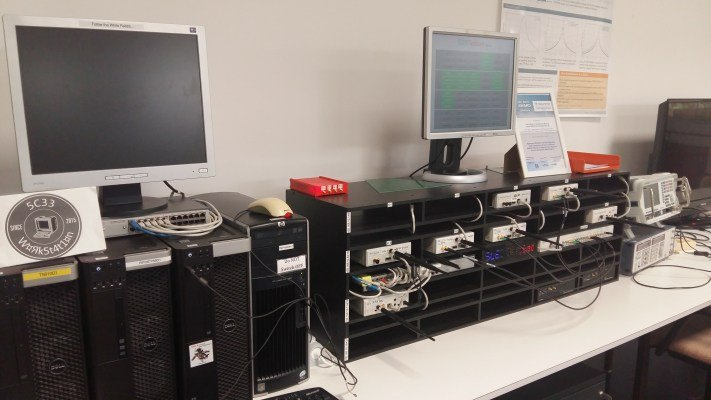
\includegraphics[width=0.70\linewidth]{SCEE_TestBed1.jpg}
    \vspace*{20pt}
    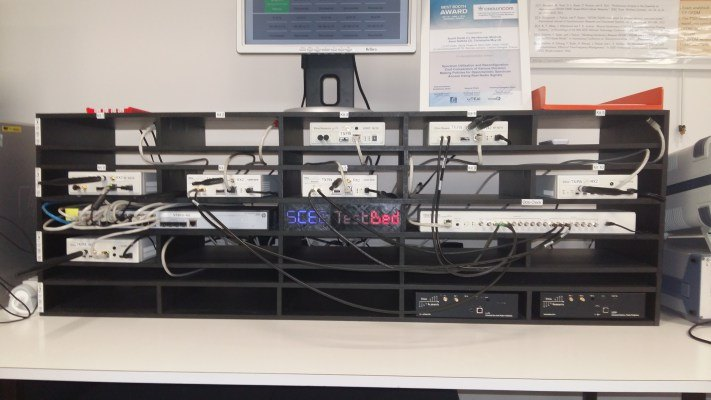
\includegraphics[width=0.70\linewidth]{SCEE_TestBed2.jpg}
    \caption{Two pictures showing the SCEE testbed \cite[Appendix~3]{Bodinier17}, taken in $2018$.}
    \label{fig:42:photosSCEETestBed}
\end{figure}

The boards have their own power supply, and are all connected to a local Ethernet switch, itself connected to a single laptop, running GNU/Linux and Ubuntu.
The pictures in Figure~\ref{fig:42:photosSCEETestBed} show the testbed used for these experiments.
% Octoclock
To ease the synchronization in both time and frequency between the boards representing the dynamic devices and the base station, we use an Octoclock \cite{OctoclockProduct}, also a product of Ettus Research,
% https://www.ettus.com/product/details/OctoClock-G
and coaxial cables connecting every platform to the Octoclock for time (PPS) and frequency synchronization, but this is not mandatory.


\paragraph{Details about our implementation.}
%
We used the GNU Radio Companion software (GRC, version $3.7$ in $2017$),
and a laptop runs a GRC design to configure and control each USRP platform.
As such, one laptop can run in parallel the control program of any number of boards\footnote{~Even if in practice, maximum efficiency is kept as long as there is not more than one GRC design by CPU core.}.
%
The GNU Radio software provides the framework and tools to build and run software radio or just general signal-processing applications.
GNU Radio applications are flow-graphs: a series of signal processing blocks connected together to describe a data flow.
For maximum efficiency, we wrote all of our blocks in \texttt{C++}.
These flow-graphs can be written in either \texttt{C++} or the Python programming language. The GNU Radio infrastructure is written entirely in \texttt{C++}, and many of the user tools are written in Python.
GNU Radio Companion is a graphical user interface (UI) used to develop GNU Radio applications:
GRC is effectively a Python code-generation tool.
When a flow-graph is compiled in GRC, a Python code is produced, which can be executed to connect to the USRP,
create the desired GUI windows and widgets, and create and connect the blocks in the flow-graph.

Illustrations of the flow-graph for the three components of the presented demonstration are included in Appendix~\ref{sec:4:IllustrationFlowcharts}, in Figures~\ref{fig:4app:USRP_TX_PU__v1__simple_grc}, \ref{fig:4app:USRP_RX_BTS__v1__simple_grc} and \ref{fig:4app:USRP_TX_SU__v1__simple_grc}.


\paragraph{User Interface.}

We have designed a user interface in order to visualize the results obtained  with our experimental demonstration. This user interface is shown in Figure~\ref{fig:42:UI}.
We can see that it is made of three parts, one for each USRP, as highlighted in \textcolor{darkred}{circled red numbers}.

\begin{figure}[!h]
    \centering
    
\includegraphics[width=1.00\textwidth]{UI.eps}
    \caption{User interface of our demonstration.}
    \label{fig:42:UI}
\end{figure}


\begin{enumerate}[label=\textcolor{darkred}{\protect\boldcircled{\arabic*}},leftmargin=6mm]
    \item %[(1)]
    % \item[\textcolor{darkred}{\circled{1}}]
The first part is the interface of the IoT traffic generator, where we see the traffic generated by this USRP, presented in a waterfall view in the time vs frequency domain.
Messages of the random traffic, generated by surrounding static devices, are shorter in time by purpose (they could be coming from other IoT standard), in order to distinguish them from an intelligent device traffic on the ``waterfall'' visualizations of the traffic.

    \item %[(2)]
    % \item[\textcolor{darkred}{\circled{2}}]
The second part is the interface of the intelligent device which is made of four parts.
At the top left, we observe the constellation of the transmitted packet \circled{a}.
At the bottom left, we have a time/frequency view of the lasts packets transmitted by the device \circled{b}.
We can see, in this view that the device transmitted its last $9$ packets in channels $\#3$ and $\#4$.
Then, at the top right of this interface \circled{c}, we can see the traffic observed by this device, where we have the interfering traffic (\textcolor{darkgreen}{green}), the uplink packets transmitted by this device (\textcolor{darkred}{red}) and the acknowledgements sent by the base station (\textcolor{darkblue}{blue}).
Colors in the ``waterfall'' represent the RF power level received at the device antenna. Hot colors are for closer elements, as for instance the device Tx antenna (reception) is close to the device Rx antenna (transmission), and consequently for the device waterfall these signals are colored in \textcolor{darkred}{red} (see graph \circled{c} in part \textcolor{darkred}{\boldcircled{2}}).
Finally, at the bottom right \circled{d}, we have four histograms showing the performance indicators of the chosen MAB algorithm (number of transmissions, number of successful transmissions, UCB indexes and success rates, in each channel).

    \item %[(3)]
    % \item[\textcolor{darkred}{\circled{3}}]
The last part is the interface of the base station, where we can see the traffic observed by the base station \circled{a} and the channels in which the last acknowledgements have been sent \circled{b}.
The observed traffic is coherent with \circled{c} of part \textcolor{darkred}{\boldcircled{2}}, as the elements are very close the one from the others on the testbed. Colors may change, as they depend on the exact distance between the different transmitters and receivers. See more details in \cite{MoyBesson2019}.
\end{enumerate}


% ----------------------------------------------------------------------
\subsection{Experimental results}
\label{sub:42:results}
% ----------------------------------------------------------------------
We compare in this PoC the two algorithms described in Section~\ref{sec:2:famousMABalgorithms} (\UCB{} and Thompson sampling) against a uniform access algorithm, that uniformly selects its channel at random.
Note that we could run more algorithms, but with no real added-valued in terms of validation of the proposed learning-based approach, which is our goal.
%
For one dynamic device, three algorithms are compared by their mean successful communications rates, on a horizon of $T=2000$ communication slots, and were using three algorithms: uniform random access (in \textcolor{cyan}{cyan}), Thompson Sampling (``\textcolor{green}{TS}'', in \textcolor{green}{green}) and \UCB{} (in \textcolor{red}{red}).

\begin{figure}[!h]
	\centering
    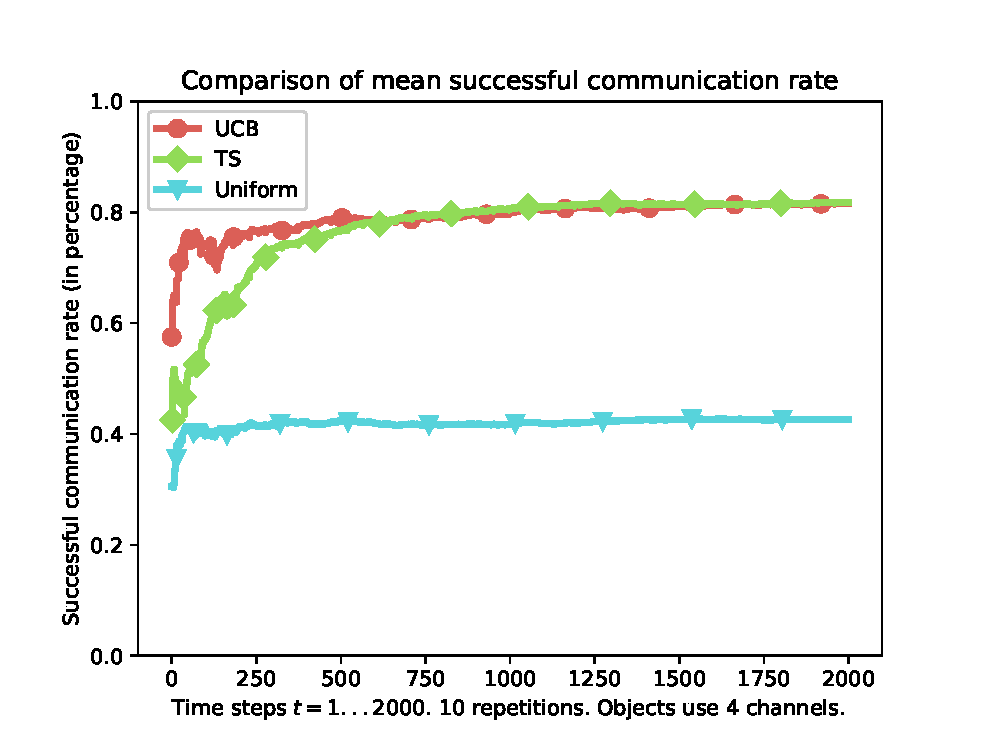
\includegraphics[height=9.0cm]{plot_datafile_append_Uniform_vs_UCB_vs_TS.eps}
    \caption{Less than $400$ communication slots (\ie, less than $100$ trials in each channel) are sufficient for the two learning devices (\textcolor{red}{\UCB} and \textcolor{green}{Thompson Sampling}) to reach a successful communications rate close to $80\%$, which is \textbf{twice as much} as the \textcolor{cyan}{non-learning (uniform)} device, which stays around $40\%$ of success. Similar gains of performance were obtained in other scenarios.}
    \label{fig:42:plot_datafile_append_Uniform_vs_UCB_vs_TS}
\end{figure}

In Figure~\ref{fig:42:plot_datafile_append_Uniform_vs_UCB_vs_TS} below, we show the results averaged on $10$ repetitions using the same conditions.
%
Each experiment has been done on a duration of about half a day,
due to the IoT sporadic transmission mode that we want to respect (like in our model of Section~\ref{sec:4:firstModel}).
However, we make devices generate one message every $5$ seconds, in order to artificially speed up the process and with no loss of generality (as we are using real hardware).
Learning can be useful only when there is a large enough difference between ``good'' and ``bad'' channels,
Each device was learning to access $4$ different non-overlapping channels, that we chose to have occupancy rates of $(\mu_k)_k = [15\%, 10\%, 2\%, 1\%]$.
Note that a maximum occupancy rate of $15\%$ could seem not so high, but indeed it is, because for a pure ALOHA access mode, a naive dynamic device only enjoys about $40\%$ success rate, under such occupancy of the channels (see the ``uniform'' plot in Figure~\ref{fig:42:plot_datafile_append_Uniform_vs_UCB_vs_TS}).
%
The occupancy rate of a channel, which denotes the mean occupancy, is implemented using the traffic generator, to emulate the presence of $S_i$ static devices with emission probability $p$ (that is, $\mu_i = S_i \times p$ here).

% They did not overlap each other, as
When facing the same stationary background traffic, we see that the learning devices are both quickly more efficient than the naive uniform device.
We obtain an improvement in terms of successful communications rate from $40\%$ to about $60\%$ in only $100$ communications (about $16\;\mathrm{min}$), and up-to $80\%$ in only $400$ communications.
%
In stationary environments, both the TS and \UCB{} algorithms are efficient and converge quickly, resulting in a strong decrease in collisions and failed communication slots. \UCB{} is faster to learn but eventually TS gives a (slightly) better average performance.

Similar results are obtained for overlapping channels, when dynamic devices are learning in the presence of multiple devices, all using the same learning algorithm.
However, our experimental testbed can not run hundreds of intelligent devices.
Empirical results confirm the simulations presented in Section~\ref{sec:4:firstModel} (see Figure~\ref{fig:41:perf_learning}).
Such results are very encouraging, and illustrate well the various strong possibilities of MAB learning applied to IoT networks.

% \begin{figure}[!t]
% 	\centering
%     \begin{subfigure}[b]{0.46\textwidth}
%         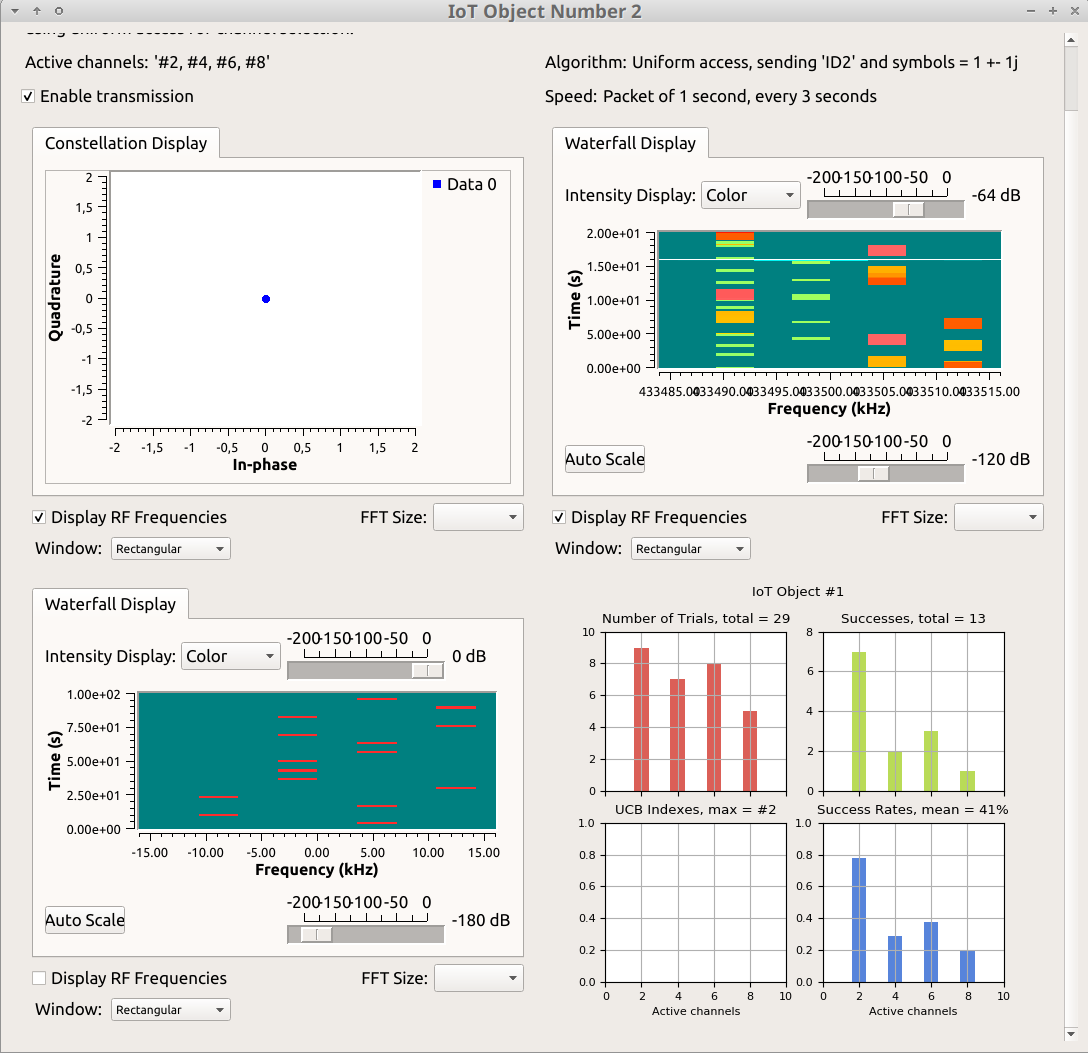
\includegraphics[height=7cm]{Object2_UniformAccess__UI.png}
%         %\caption{Device using uniform access.}
%         \label{fig:42:comparing_UniformAccess_and_UCB__1}
%     \end{subfigure}
%     ~ %add desired spacing between images, e. g. ~, \quad, \qquad, \hfill etc.
%       %(or a blank line to force the subfigure onto a new line)
%     \begin{subfigure}[b]{0.46\textwidth}
%         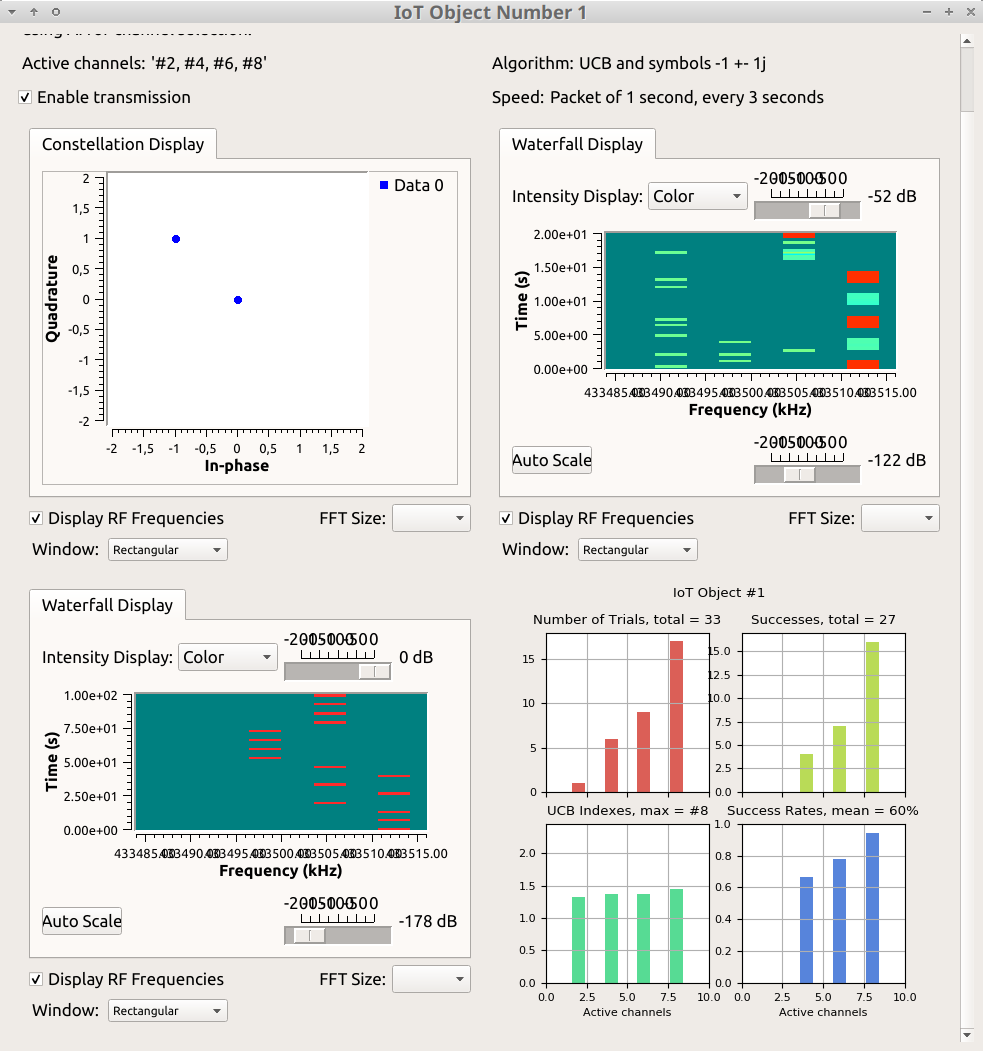
\includegraphics[height=7cm]{Object1_UCB__UI.png}
%         %\caption{Device using UCB.}
%         \label{fig:42:comparing_UniformAccess_and_UCB__2}
%     \end{subfigure}
% \caption{Comparing the success rate of an device using uniform access (left, $41\%$ of success here) and an device using the UCB algorithm (right, already $60\%$ of success). We see the learning device being much more present in the channels $\#4$ and $\#3$ (\textcolor{darkblue}{blue chart}, bottom right corner), as these channels are the less perturbed by the random interfering traffic, in this example.}
% \label{fig:42:comparing_UniformAccess_and_UCB}
% \end{figure}


\paragraph{Availability of data and materials.}
%
The source code of our demonstration is fully available online, open-sourced under GPLv3 license, at
\href{https://bitbucket.org/scee_ietr/malin-multi-arm-bandit-learning-for-iot-networks-with-grc}{\texttt{bitbucket.org/scee\_ietr/malin-multi-arm\\-bandit-learning-for-iot-networks-with-grc/}}.
%
It contains both the GNU Radio Companion flowcharts and blocks, with ready-to-use \texttt{Makefiles} to easily compile, install and launch the demonstration.
The demonstration only requires a laptop and open-source free softwares,
as the laptop should run a GNU/Linux distribution (like Ubuntu or Debian),
in addition to USRP platforms from Ettus Research.


\paragraph{Video.}
%
As depicted in Figure~\ref{fig:42:screenshotDemoYouTube} below,
we realized a $6$-minute \textbf{video} to sum-up our demonstration and advertise our work online, and it is available on the YouTube hosting platform, at \texttt{\href{https://youtu.be/HospLNQhcMk}{youtu.be/HospLNQhcMk}}.
The video shows examples of $3$ dynamic devices learning simultaneously, confirming the results of Figure~\ref{fig:42:plot_datafile_append_Uniform_vs_UCB_vs_TS} for overlapping channels.
It also shows the connections between the USRP boards, the Octoclock, the master laptop etc, completing the presentation of the SCEE testbed already shown in Figure~\ref{fig:42:photosSCEETestBed}.
% \textcolor{white}{Of course, the video was not seen much, because our work is useless! Yay!}

\begin{figure}[!h]
	\centering
    % \includegraphics[width=0.90\textwidth]{Images/screenshotDemoYouTube.png}
    \includegraphics[width=0.90\textwidth]{2-Chapters/4-Chapter/Images/screenshotDemoYouTube.png}
    \caption{Screenshot of the \textbf{video} of our demonstration, \texttt{\href{https://youtu.be/HospLNQhcMk}{youtu.be/HospLNQhcMk}}.}
    \label{fig:42:screenshotDemoYouTube}
\end{figure}

% \paragraph{Special acknowledgment.}
% %
% We acknowledge the work of two engineering students, at CentraleSup{\'e}lec campus of Rennes,
% Cl{\'e}ment Barras and Th{\'e}o Vanneuville, for their GNU Radio project in Spring $2017$,
% as we took inspiration in the GNU Radio code and the discussions we had at this time.




\newpage  % WARNING ?
% ----------------------------------------------------------------------------
\section{Extending the model to account for retransmissions}
\label{sec:4:retransmissions}
% ----------------------------------------------------------------------

% - ``Upper-Confidence Bound for Channel Selection in LPWA Networks with Retransmissions'', see \texttt{https://perso.crans.org/besson/articles/BMBM\_\_IEEE\_WCNC\_2019.pdf}

% - ``Upper-Confidence Bound for Channel Selection in LPWA Networks with Retransmissions'', see  https://hal.inria.fr/hal-02049824

\graphicspath{{2-Chapters/4-Chapter/IEEE_WCNC__2019__Paper__BMBM.git/}}

In this section, we extend the previous model to take into account the possibility for retransmissions of a message after a collision.
This is of major importance as most protocols for real-world IoT networks can use retransmissions, it is for instance the case of the LoRaWAN standard.
As before, we propose and evaluate different learning strategies based on MAB algorithms.
However, the price to be paid is a shorter battery lifetime for IoT devices. So this approach would be used only for devices with strong delivery constraints (\eg, for health-care applications), or that can refuel their energy over time (\eg, for robotic applications).

The presented strategies allow IoT devices to improve their access to the network and their autonomy, while taking into account the impact of encountered radio collisions.
For that end, several heuristics employing \UCB{} algorithms are examined, to explore the information provided by the number of retransmissions.
In this section, our results show that approaches based on \UCB{} obtain a significant improvement in terms of successful transmission probabilities, compared to a naive approach which does not learn.
Furthermore, it also reveals that a pure \UCB{} channel access is as efficient as more sophisticated learning strategies.

% \TODOL{This section is based on the publication ``Upper-Confidence Bound for Channel Selection in LPWA Networks with Retransmissions'', see \texttt{https://hal.inria.fr/hal-02049824}}

% https://hal.inria.fr/hal-02049824


% % ----------------------------------------------------------------------
% \subsection{Retransmissions in an ALOHA like protocol}
% \label{sub:43:introduction}
% % ----------------------------------------------------------------------

% In the context of Cognitive Radio \cite{Mitola99,Haykin05},
% Multi-Arm Bandit (MAB) algorithms \cite{Auer02,Auer02,Bubeck12} have been recently proposed as a potential solution for channel access in LPWA networks \cite{Bonnefoi18,Azari18,Bonnefoi17}.
We presented in Section~\ref{sec:4:firstModel} the impact of non-stationarity on the network performance using MAB algorithms is studied.
Low-cost algorithms following two well-known approaches, such as the Upper-Confidence Bound (\UCB{}), and the Thompson Sampling (TS) algorithms have reported encouraging results.
When considering the application of MAB algorithms for slotted wireless protocols in a decentralized manner,
other recent directions of research include theoretical analysis, like what we present in the next Chapter~\ref{chapter:5},
or realistic empirical PoC like in \cite{MoyWSR2014,RobertSDR2014,modiDemo2016,darak2016bayesian,kumar2016two,kumar2017channel} or the previous Section~\ref{sec:4:gnuradio},
and finally applications to multi-hoping networks \cite{Mitton16,Toldov16} or other kinds of networks \cite{Wilhelmi19collaborative,Wilhelmi19potential}.
%
None of the mentioned works discuss in detail the impact of retransmissions on the performance of MAB learning algorithms as we do now.

The aim of this section is to assess the performance of MAB algorithms for channel selection in LPWA networks operating in unlicensed bands, while taking into account the impact of retransmissions on the network performance.
For this reason, several decision making strategies are applied after a first retransmission (\ie, when a collision occurs).
The proposed approach employs contextual information provided by the number of retransmissions, and is again implemented independently by each device, so that no coordination among them is needed.
Moreover, our \UCB{}-based heuristics show low complexity making them suitable for being embedded in LPWA devices.

The contributions of this section are summarized as follows.
% \begin{itemize}
	% \item
	Firstly, we provide a close form approximation of the radio collision probability after a first retransmission.
	By doing this, we highlight the need to develop a learning approach for channel selection upon collision.
%
	% \item
	Secondly, different heuristics are proposed to cope with retransmissions.
%
	% \item
	Lastly, we conduct simulations in order to compare the performance of the proposed heuristics with a naive uniform random approach, and a \UCB{} strategy (\ie, without any learning for the retransmissions, that is, the same channel is used for retransmission).
% \end{itemize}


% \textbf{Outline.}
% %
% The rest of the section is organized as follows.
% First the system model is introduced in Section~\ref{sub:43:model},
% and our motivations are exposed in Section~\ref{sub:43:motivations}.
% The proposed \UCB-based heuristics are presented in Section~\ref{sub:43:heuristics}, while the corresponding numerical results are shown in Section~\ref{sub:43:numExp}.
% Finally, some conclusions are drawn later in Section~\ref{sub:43:conclusion}.


% ----------------------------------------------------------------------
% \subsection{Extending our model with retransmissions}
\subsection{Presentation of the model with retransmissions}
\label{sub:43:model}
% ----------------------------------------------------------------------

% ----------------------------------------------------------------------
\paragraph{LPWA network.}

Like before in this chapter, we consider an LPWA network composed of a gateway and a large number of end-devices that regularly send short data packets, where $K$ channels ($K>1$) are available for the transmission of their packets.
%
We assume that this network is constituted by two types of devices:
On the one hand, we have \emph{static} devices that operate in one channel\footnote{~Note that, for unlicensed bands, this definition also encompasses any device following a different standard or trying to establish communication with gateways of other networks.} in order to communicate with the gateway.
%
On the other hand, there are  IoT devices, that possess the additional advantage of being able to select any of the $K$ available channels to perform their transmissions.

Like in the previous model presented in Section~\ref{sec:4:firstModel},
regardless the type of devices, each of them follows a slotted ALOHA protocol \cite{Roberts75}, and has a probability $p>0$ to transmit a packet in a time slot.
We make the hypothesis that the transmission is successful if the channel is available, otherwise it fails upon radio collision.
The novelty compare to the previous model is that
in case of RF (uplink or downlink) collision that prevent the device to receive the \emph{Ack} from the gateway,
these devices will attempt to retransmit their packet up-to $\mathrm{MaxBackOff}$ times\footnote{~We denote it $\mathrm{MaxBackOff}$ instead of $M$ like we did in our paper \cite{Bonnefoi2019WCNC}, as $M$ is used in next Chapter~\ref{chapter:5}.},
with $\mathrm{MaxBackOff} \in\mathbb{N}^*$.
It is important to note that, every retransmission is carried out after a random back-off time, uniformly distributed in $\{0, \dots, m-1\}$, where $m \in\mathbb{N}^*$ is the length of the back-off interval
(note the difference between $m$ and $\mathrm{MaxBackOff}$).


% ----------------------------------------------------------------------
\paragraph{Model of IoT devices.}

The aforementioned contention process can be described by a Markov chain model \cite{Norris98} similar to the one presented in \cite{Yang12}, as it is depicted in Figure~\ref{fig:43:Markov_model}.
When a device has a packet to transmit, it goes from an idle state to a transmission state, while considering retransmissions due to different collision probabilities, $\{p_{c}, p_{c1}, \dots, p_{\mathrm{MaxBackOff}-2} \}$, at each $\mathrm{MaxBackOff}$ back-off stage.
At each time slot, a transition from an idle state to a transmission state (denoted as \texttt{Trans.}) occurs if a packet transmission is required, while waiting states (denoted as \texttt{Wait}), correspond to a $m$ back-off interval.

\begin{figure}[!h]
	\centering
	\includegraphics[width=0.70\linewidth]{Markov_model.eps}
	% \includegraphics[width=0.70\linewidth]{Markov_model-eps-converted-to.pdf}
	\caption{The Markov model of the behavior of all devices paired to the considered IoT network using the ALOHA protocol.}
	\label{fig:43:Markov_model}
\end{figure}

A device aims to select a channel with the highest probability of successful transmissions, for which it uses a reinforcement learning approach, again formulated as a MAB problem.
Contrarily to what may appear at first sight,
\emph{the goal is not to minimize the number of retransmissions}, but to maximize the probability of successful transmission, considering both the first transmission of a message and the retransmissions of the same message.
Indeed, the objective of each device is to \emph{maximize its battery life by minimizing its \textbf{total} number of transmissions}.
% , where each channel (also called arms) is viewed as a gambling machine (bandit), and each bandit has a \emph{reward}. Then, at every trial, a device chooses a channel that maximizes the sum of the collected rewards. These \emph{rewards} are the \emph{acknowledgment} (\emph{Ack}) signals received after transmitting packets to the gateway. In this way, a transmission is considered successful when an acknowledgment is received, and a learning approach is employed to select the best channel.
%
We address the problem of channel selection taking into account the described Markov model for the retransmissions of end-devices.
% It motivates our present work for which we consider the retransmissions in the analysis of MAB algorithms.
It motivates our present work for which we consider the number of retransmissions, carried out by each device.
% to address several MAB algorithms.
%

% ----------------------------------------------------------------------
\subsection{Motivations for the proposed approach}
\label{sub:43:motivations}
% ----------------------------------------------------------------------

We consider IoT devices with a constraint on their QoS, imposing the successful delivery of their messages.
When such an IoT device experiments a collision, it goes in a back-off state to retransmit the same packet on the same or another channel.
If all devices remain in the same channel for retransmissions, it is a well-known result that it could result in a sequence of successive collisions with the same packets' devices that previously collided.
%
Thus, it seems interesting to consider in the decision making policy the possibility for a device to retransmit in a different channel.
One of our motivations to develop new MAB algorithms for our problem is this option of using a different communication channel between the first transmission and the next retransmissions.

By considering this possibility, the device will have to learn more, thus, we expect the learning time to be longer, but it could be possible that the final performance gain increases too, in terms of network performance.
We present in Section~\ref{sub:43:numExp} an analysis to check this performance gain, for various heuristics based on the \UCB{} algorithm.
%
Here after, we start by presenting a mathematical derivation that backups this idea.
To do so, we study the collision probabilities considering the Markov process depicted in Figure~\ref{fig:43:Markov_model}, and foresee the impact of using bandit strategies, as well as setting guidelines for the design of heuristic approaches.


\paragraph{Probability of collision at a second transmission slot.}

It is well known \cite{Abramson1970,Roberts75}
that having a collision during an access time can be overcome by a retransmission procedure (this can take several retransmission attempts).
Our goal here is to obtain a mathematical approximation of the collision probability at the second transmission slot $p_{c1}$, as a function of the first collision probability $p_{c}$.
%
We make two approximations $\mathcal{H}_{1}$ and $\mathcal{H}_{2}$ defined as (they are hypotheses on which the rest of this section is built),
\begin{itemize}
	\item $\mathcal{H}_{1}$:
    The probability $p_{c1}$, is composed by the sum of two probabilities: i)
    the probability of colliding consecutively twice, \ie, the devices that collide at a given time slot and collide again when retransmitting their packets,
	and ii) the probability of collision among devices that did not collide in the same previous collision. Moreover, we suppose that the number of devices involved in a collision is small in comparison to the total number of devices.
	This is very realistic as a very small proportion of devices transmit at the same period, due to their low duty cycle.

	\item $\mathcal{H}_{2}$:
	The total number of back-off stages at time $t$ is constant, and it is assumed to be large enough to consider that no device will ever be in the last failure state (this case is the one on the right side in Figure~\ref{fig:43:Markov_model}), after $\mathrm{MaxBackOff}$ successive failed retransmissions
	(otherwise, its battery life can be threatened if it does not have re-fueling capabilities).
\end{itemize}

Considering one device and one channel,
we denote $x_t^i$ the probability that it is transmitting a packet for the $(i+1)$-th time in a given time slot $t$ (with $i\in \{0, \dots, \mathrm{MaxBackOff}-1 \}$),
and we denote $x_t = \sum_{i=0}^{\mathrm{MaxBackOff}-1}x_t^i$ the probability that it transmits a packet (\ie, just the sum on $i$ of $x_t^i$).
We consider $N > 0$ active devices following the same policy.

%{\color{red}Considering one device and a channel,
%we denote $x_t^i$ the packet transmission probability for the $i+1$ time in a given time slot $t$ (with $i\in \llbracket 0, \mathrm{MaxBackOff}-1 \rrbracket$).}
%
%{\color{red}Considering one device and a channel, we denote $x_t^i$ the transmission probability for the $i+1$ time, with $i\in \llbracket 0, \mathrm{MaxBackOff}-1 \rrbracket$, in a given time slot $t$}

We assume to be in the steady state \cite{Norris98}, in our Markov chain model depicted in Figure~\ref{fig:43:Markov_model}, and thus the probabilities no longer depend on the slot number $t$ (\ie, $\forall t, x_t=x$).
Therefore, the probability that this device has a collision at the first transmission is $p_c$, and has the following expression
%
\begin{equation}\label{eq:43:1}
	p_c = 1-\left(1-x\right)^{N-1} \iff x = 1-\left(1-p_c\right)^{\frac{1}{N-1}}.
\end{equation}

Moreover, from \eqref{eq:43:1} we define the probability $p_{cp}(n)$ that involves the collision of $n$ packets sent by each IoT device (for any $1\leq n \leq N-1$), during the first transmission slot, and is defined by $p_{cp}(n) = {N-1 \choose n} \; x^n \left(1-x\right)^{N-1-n}$.
%
As explained above, if an IoT device experiences a collision at the first transmission, it proceeds for the retransmission of its packet after a random back-off interval.
We denote $p_{ca}$ the probability to have a collision with a packet involved in the previous collision.
Under the $\mathcal{H}_{1}$ assumption, the number of packets involved in the same previous collision remains very small in comparison to the total number of devices that may transmit during this time. In other words, this collision probability does not depend on previous retransmissions and is equal to $p_c$.
So, the probability that the same device's packet experiences again a collision at the second time slot is
%
\begin{equation}\label{eq:43:decomppc1}
	p_{c1} = p_{ca}+\left(1-p_{ca} \right)p_c.
\end{equation}


If the device has a collision at the first attempt, we consider $p_{bp}(n)$ the probability that it has a collision with \emph{exactly} $n$ packets (for any $1\leq n \leq N-1$), and that \emph{at least one} of the $n$ devices involved in this first collision chooses the same back-off interval,
%
\begin{equation}
    p_{bp}(n) = {N-1 \choose n} x^n \left(1-x\right)^{N-1-n}\left[1-\left( 1-\frac{1}{m}\right)^n \right].
\end{equation}


Besides, $p_{ca}$ is the conditional probability of collision with a packet sent by a device involved in the previous collision given that the packet experienced collision at its first transmission.
Hence, under hypothesis $\mathcal{H}_{2}$, we can use Bayes theorem and the law of total probability to relate $p_{ca}$ with $p_{bp}(n)$, and the different probabilities that a device experienced a collision during the first slot and has the same back-off interval for its retransmission is,
%{\color{red}Hence, under hypothesis $\mathcal{H}_{2}$,
%the collision probability with the same packets after a retransmission, $p_{ca}$, is given  the sum of collision probabilities with $n$ devices choose the same back-off interval for their retransmissions, }
%
% \begin{equation}\label{eq:43:sumpca}
	$p_{ca} = \frac{1}{p_c}\sum_{n=1}^{N-1} p_{bp}(n)$.
% \end{equation}
%
% \begin{figure}[htp!]  % [htbp]
% 	\centering
% 	% \includegraphics[width=1.00\linewidth]{Approximation_m10.eps}
% 	\includegraphics[width=1.00\linewidth]{Approximation_m10-eps-converted-to.pdf}
% 	\caption{Our proposed approximation for the probability of collision at the second transmission. It is more precise for smaller values of $N$.}
% 	\label{fig:43:Approximation_m10}
% \end{figure}
%
Therefore, the expression of $p_{ca}$ is
%
\begin{align}\label{eq:43:sumpc2}
	& \frac{1}{p_c} \sum_{n=1}^{N-1}{N-1 \choose n} x^n \left(1-x\right)^{N-1-n}\left[1-\left( 1-\frac{1}{m}\right)^n \right]\nonumber \\
	& = 1- \frac{1}{p_c}\sum_{n=1}^{N-1}{N-1 \choose n} x^n \left(1-x\right)^{N-1-n}\left( 1-\frac{1}{m}\right)^n.
\end{align}

Once again under $\mathcal{H}_{1}$, assuming that the number of devices involved in the first collision is small compared to $N-1$, the first $N_0 \ll N-1$ terms of the sum in \eqref{eq:43:sumpc2} are predominant. We derive $p_{ca} \simeq  1- \frac{1}{p_c}\sum_{n=1}^{N_0}{N-1 \choose n} x^n\left(1-x\right)^{N-1-n} \left( 1-\frac{1}{m}\right)^n$.
%
Moreover, for these terms, $n$ is small compared to $N-1$, and so $N-1-n$ can be approximated to $N-1$. Thus it gives,
%
\begin{equation}\label{eq:43:sumpca3}
	p_{ca} \simeq  1- \frac{\left(1-x\right)^{N-1}}{p_c}\sum_{n=1}^{N_0}{N-1 \choose n} x^n \left( 1-\frac{1}{m}\right)^n.
\end{equation}

Assuming $\mathcal{H}_{1}$ amounts to consider that $x\ll 1$. As a consequence, the sum in equation \eqref{eq:43:sumpca3} can be supplemented by negligible terms,
%
\begin{equation}\label{eq:43:sumpca4}
	p_{ca} \simeq  1 - \frac{\left(1-x\right)^{N-1}}{p_c}\sum_{n=1}^{N-1}{N-1 \choose n} x^n \left( 1-\frac{1}{m}\right)^n.
\end{equation}

The binomial theorem expands the sum in \eqref{eq:43:sumpca4}, so we can rewrite the expression of $p_{ca}$ as
%
\begin{equation}\label{eq:43:pca}
	p_{ca} \simeq 1 - \left(\frac{1}{p_c}-1\right)\left[ 1+\left(1-\left(1-p_c\right)^{\frac{1}{N-1}}\right)\left(1-\frac{1}{m}\right)\right]^{N-1}.
\end{equation}

Finally, our approximation of $p_{c1}$ can be obtained by inserting \eqref{eq:43:pca} in \eqref{eq:43:decomppc1}.
%
\begin{align}\label{eq:43:final_expression_pc1}
	p_{c1} &= p_{ca}+\left(1-p_{ca}\right)p_c = (1 - p_c) p_{ca} + p_c \nonumber \\
	&\simeq \left(1 - p_c\right) (1 - \left(\frac{1}{p_c}-1\right)\left[ 1+\left(1-\left(1-p_c\right)^{\frac{1}{N-1}}\right)\left(1-\frac{1}{m}\right)\right]^{N-1} + p_c.
\end{align}


% --- --- --- --- --- --- --- --- --- ---
\paragraph{Behavior analysis of $p_{c}$ and $p_{c1}$}\label{sub:43:numericalValidationPC1PC}

In order to assess the proposed approximation, we suppose a unique channel where all the devices follow the same contention Markov process.
We simulate an ALOHA protocol with a maximum number of retransmissions $\mathrm{MaxBackOff}=10$, a maximum back-off interval $m=10$, and a transmission probability $p=10^{-3}$.
%
In Figure~\ref{fig:43:Approximation_m10}, we show the collision probabilities for different number of devices $N$ (from $N=50$ up-to $N=400$), for both $p_{c}$ and $p_{c1}$.
%
From this simulations, we can verify that our approximation is very precise for lower values $p_{c1} \leq 30 \%$ (\ie, red and orange curves are quite close).
Moreover, a significant gap between $p_{c1}$ and $p_c$,
of up-to $10\%$, can be observed,
which suggests us to resort to MAB algorithms for the channel selection for both the first transmission and next retransmissions.

\begin{figure}[htp!]  % [htbp]
	\centering
	% \includegraphics[width=0.65\linewidth]{Approximation_m10.eps}
	\includegraphics[width=0.70\linewidth]{Approximation_m10-eps-converted-to.pdf}
	\caption[Proposed approximation for the probability of collision at the second transmission]{Proposed approximation for the probability of collision at the second transmission. It is more precise for smaller values of $N$.}
	\label{fig:43:Approximation_m10}
\end{figure}


\paragraph{Learning is useful for non-congested networks.}

It is worth to highlight that, if we write \eqref{eq:43:decomppc1} as $p_{c1} = p_c + p_{ca} \left(1-p_c\right)$,
then it is obvious that $p_{c1}$ is always larger than $p_c$ (as $p_{ca} \left(1-p_c\right) > 0$).
But for large values of $p_c$, $p_{ca}\left(1-p_c\right) \simeq 0$ so the gap gets small,
and for small values of $p_c$ the gap is significant.
Moreover, we can verify (\eg, numerically or by differentiating)
that the gap decreases when $p_c$ increases (for fixed $N$ and $m$).
This backups mathematically the observation we made from Figure~\ref{fig:43:Approximation_m10}:
the smaller the $p_c$, the larger is the gap between $p_c$ and $p_{c1}$.

We interpret this fact in two different situations:
\begin{itemize}
	\item
	On the one hand, in a congested network, when devices suffer from a large probability of collision on their first transmission (\ie, $p_c$ is not so small), then $p_{c1}\simeq p_c$ and so devices cannot really hope to reduce their collision probabilities even if the use a different channel for retransmission.
	\item
	On the other hand, if $p_c$ is small enough, \ie, in a network not yet too congested, then our derivation shows that $p_{c1} > p_c$, meaning that the possible gain of retransmitting in a different channel that the one used for the first transmission can be large, in terms of collision probability (\eg, up-to $10\%$ in this experimental setting).
	In other words, when learning can be useful (small $p_c$), learning to retransmit in a different channel can have a large impact on the global collision rate,
	thus justifying our approach.
\end{itemize}

% %-----------------------------------------------------------------
% \subsection{The \UCB{} algorithm as a building block for different heuristics}
% \label{sub:43:MABalgo}
% % ----------------------------------------------------------------------

% Before presenting our proposed heuristics, we remind here the \UCB{} bandit algorithm \cite{Auer02}.
% We include it again to facilitate the understanding of the heuristics, which use \UCB{} as a building block.


% % % --- --- --- --- --- --- --- --- --- ---
% \paragraph{The \UCB{} algorithm.}\label{sub:43:algoUCB}

% More formally, for one device, let $N_k(t)$ be the number of times the channel $k$ (for $k\in \llbracket 1, K \rrbracket$) was selected up-to time $t-1$, for $t\geq 0$
% for any $t\in\mathbb{N}$,
% \begin{equation}\label{eq:43:Nkt}
% 	N_k(t) = \sum_{\tau=0}^{t-1} \mathbbm{1}(A(\tau) = k),
% \end{equation}
% The empirical mean estimator $\widehat{\mu_k}(t)$ of channel $k$ is defined as the mean reward obtained up-to time $t-1$,
% \begin{equation}\label{eq:43:mukt}
% 	\widehat{\mu_k}(t) = \frac{1}{N_k(t)} \sum_{\tau=0}^{t-1} r_k(\tau) \mathbbm{1}(A(\tau) = k).
% \end{equation}
% where $r_{k}(t)$ is the reward obtained after transmission in channel $k$ at time $t$ ($1$ for a successful transmission, and $0$ otherwise)
% %
% A \emph{confidence} term $B_k(t)$ is given by \cite{Auer02},
% \begin{equation}\label{eq:43:Bkt}
% 	B_k(t) = \sqrt{\alpha \log(t) / N_k(t)},
% \end{equation}
% where $\alpha$ refers to an exploration coefficient,
% % \footnote{~In fact, the larger this coefficient is, the longer the exploration, while the \UCB{} algorithm is proven to be order optimal for $\alpha>0.5$ \cite{Bubeck12}, and has reported a good performance for lower values of $\alpha>0$.},
% that we chose equal to $1/2$, as suggested in \cite{Audibert07} and as done in previous works \cite{Bonnefoi18,Bonnefoi17}.
% Then, an upper confidence bound in each channel $k$ is defined as
% \begin{equation}\label{eq:43:ucb}
% 	U_k(t) = \widehat{\mu_k}(t) + B_k(t).
% \end{equation}
% Finally, the transmission channel at time step $t$
% is the one maximizing this \UCB{} index $U_k(t)$,
% as it is the one expected to be the best one at the current time step $t$,
% \begin{equation}\label{eq:43:maxucb}
% 	A(t) \sim \cU(\argmax_k U_k(t)).
% \end{equation}

% The \UCB{} algorithm is implemented independently by each device, and we present it in Algorithm~\ref{algo:43:UCB}.
% Note that a device using this first approach is only able to select a channel for the first and all the corresponding retransmissions of a packet.

% % \begin{small} % XXX remove if needed
% \begin{figure}[h!]
% 	\centering
%     \begin{framed}
% 	\begin{algorithm}[H]
		% \begin{small} % XXX remove if needed
% 		\For(){$t = 1, \dots, T$}{
% 			Compute $\forall k, U_k(t) = \widehat{\mu_k}(t) + \sqrt{\alpha \log(t) / N_k(t)}$\;
% 			Transmit in channel $A(t) \sim \cU(\argmax_k U_k(t))$\;
% 			Reward $r_{A(t)}(t) = 1$, if \emph{Ack} is received, else $0$\;
% 		}
% 		\caption{The \UCB{} algorithm for channel selection (base building block).}
% 		\label{algo:43:UCB}
		% \end{small} % XXX remove if needed
% 	\end{algorithm}
% 	\end{framed}
% \end{figure}
% % \end{small} % XXX remove if needed

% ----------------------------------------------------------------------
\subsection{The first heuristic: \UCB{} unaware of retransmissions}
\label{sub:43:UCBnaive}
% ----------------------------------------------------------------------

% \paragraph{First stage \UCB.}\label{sub:43:firstStageUCB}

This first heuristic we propose is unaware of retransmission: the same channel is used for retransmissions.
The \UCB{} algorithm is implemented independently by each device, we denote it ``first-stage'' \UCB, and we present it in Algorithm~\ref{algo:43:UCB}.
It is the same algorithm as the Algorithm~\ref{algo:2:indexPolicy} in Section~\ref{sub:2:IndexPolicies} (using the same \UCB{} indexes as we defined them in equation \eqref{eq:2:UCB_index}),
but we write it again to make clear the difference with first transmission and retransmission of messages.
%
Note that a device using this first approach is only able to select a channel for the first transmission (using \UCB, line 3-5), and then it uses the same channel for all the corresponding retransmissions of a packet (if retransmissions happen, line 7-8).


% \begin{small} % XXX remove if needed
\begin{figure}[h!]
	\centering
    \begin{framed}
	\begin{algorithm}[H]
		% \begin{small} % XXX remove if needed
		\For(){$t = 1, \dots, T$}{
			\uIf{First packet transmission}{
				Compute $\forall k, U_k(t) = \widehat{\mu_k}(t) + \sqrt{\alpha \log(t) / N_k(t)}$\;
				Transmit in channel $A(t) \sim \cU(\argmax_k U_k(t))$\;
				Reward $r(t) = 1$, if \emph{Ack} is received, else $0$\;
			}
			\Else(\tcp*[f]{Retransmit in same channel}){
				j $\leftarrow$ last channel selected by first-stage \UCB\;
				Transmit in channel $A(t) = j$\;
			}
		}
		\caption[First-stage \UCB{} and retransmission in same channel.]{First-stage \UCB{} and retransmission in same channel (``\textcolor{blue}{Only \UCB{}}'').}
		\label{algo:43:UCB}
		% \end{small} % XXX remove if needed
	\end{algorithm}
	\end{framed}
\end{figure}
% \end{small} % XXX remove if needed


More formally, for one device, let $N_k(t)$ be the number of times the channel $k$ (for $k\in [K]$) was selected up-to time $t-1$, for $t\geq1$
for any $t\in\mathbb{N}$,
$N_k(t) = \sum_{\tau=1}^{t-1} \mathbbm{1}(A(\tau) = k)$.
The empirical mean estimator $\widehat{\mu_k}(t)$ of channel $k$ is defined as $\widehat{\mu_k}(t) = \frac{1}{N_k(t)} \sum_{\tau=1}^{t-1} r(\tau) \mathbbm{1}(A(\tau) = k)$,
where $r(t)=Y_{k,t}$ is the reward obtained after transmission in channel $k$ at time $t$.
The upper confidence bound in each channel $k$ is defined as
$U_k(t) = \widehat{\mu_k}(t) + \sqrt{\alpha \log(t) / N_k(t)}$.
Finally, the transmission channel at time step $t$
is $A(t) \sim \cU(\argmax_k U_k(t))$.
% the one maximizing this \UCB{} index $U_k(t)$,
% as it is the one expected to be the best one at the current time step $t$,

\begin{leftbar}[warningbar]  % XXX leftbar warningbar, comment if needed
	\textbf{\textcolor{red}{Small warning about notations: local (device) time vs global (gateway) time}:}
	%
	In all the algorithms and notations presented in this Section, the time steps $t$ do not refer to the \emph{global} time steps (as seen from the gateway), but rather the current number of uplink transmissions (or retransmissions) that was carried out by the device.
	Each device wakes up whenever it has to send some data, following its random emission process (here, we propose a Bernoulli process of small probability, \eg, $p=10^{-3}$), and when it woke up, it sends its packet, and will send again for at most $\mathrm{MaxBackOff}$ times (\eg, $\mathrm{MaxBackOff}=10$) until it receives an \Ack.
	%
	In other words, the time steps $t$ in the following algorithms denote the number of time the device sent an uplink packet, and these uplink (re)transmissions can happen at different (real-world) times, more or less spread out in time, it does not matter to the learning part of this model and work.
\end{leftbar}  % XXX leftbar warningbar, comment if needed


% ----------------------------------------------------------------------
\subsection{Heuristics to (try to) learn how to retransmit efficiently}
\label{sub:43:heuristics}
% ----------------------------------------------------------------------

A device that implements the UCB algorithm is led to focus its transmissions and retransmissions in the channel which is currently identified as the best.
As explained above in Section~\ref{sub:43:motivations}, focusing in one channel could increase the collision probability in retransmissions.
We describe here the proposed heuristics for the channel selection in a retransmission. It is carried out taking into account that a device can incorporate a different channel selection strategy while being in a back-off state.
Hence, a natural question is to evaluate whether using this additional contextual information can improve the performance of a learning policy.

For that end, all of our heuristics comprise two stages:
the first stage is a \UCB{} algorithm employed for the first attempt to transmit,
and the second stage is another algorithm used for channel selections for the next retransmissions.
%
We present below four heuristics for this second stage.
Their short names (with their colors) are used in the legend on Figures~\ref{fig:43:mainExperiment1}, \ref{fig:43:mainExperiment2}), and are given in ``quotes'' in the corresponding paragraphs.


% --- --- --- --- --- --- --- --- --- ---
\textbf{Uniform random retransmission ``(\textcolor{cyan}{Random}'').}\label{sub:43:UCBthenRandom}
%
In this first proposal, the device uses a random channel selection, following a uniform distribution (on $[K]$).
It is described below in Algorithm~\ref{algo:43:UCBthenRandom}.
More precisely, the first-stage \UCB{} use rewards built from the acknowledgments that the device received or not for its first-stage transmission, but do not use any feedback about any of the retransmissions of any message.

% \vspace*{-3pt}
\begin{figure}[h!]
	\centering
    \begin{framed}
	\begin{algorithm}[H]
	% \begin{small} % XXX remove if needed
	\For(){$t = 1, \dots, T$}{
			\uIf{First packet transmission}{
				Use first-stage \UCB{} as in Algorithm~\ref{algo:43:UCB}\;
			}
			\Else(\tcp*[f]{Random retransmission}){
				Transmit in channel $A(t) \sim \mathcal{U}(1,\ldots,K)$\;
			}
		}
		\caption[Heuristic: uniform random retransmission.]{Heuristic: uniform random retransmission ``(\textcolor{cyan}{Random}'').}    % A naive
		\label{algo:43:UCBthenRandom}
	% \end{small} % XXX remove if needed
	\end{algorithm}
	\end{framed}
\end{figure}


% --- --- --- --- --- --- --- --- --- ---
\textbf{\UCB{} for retransmission (``\textcolor{purple}{\UCB{}}'').}\label{sub:43:TwoUCB}
%
Instead of applying a random channel selection for retransmission,
another heuristic is to use a second \UCB{} algorithm in the second stage.
In other words, we expect that this algorithm is able to learn the best channel to retransmit a packet.
It is described in Algorithm~\ref{algo:43:TwoUCB}, and it is still a practical approach, since the storage requirements and time complexity remains linear w.r.t. the number of channels $K$ (\ie, $\mathcal{O}(K)$).
%
Note that, we use the subscript $({}^r)$ to denote the variables
$\widehat{\mu^r}(t)$, $B^r_k(t)$ and $U^r_k(t)$,
related to the \UCB{} algorithm employed for the retransmission.

% \vspace*{-3pt}
% \begin{small} % XXX remove if needed
\begin{figure}[h!]
	\centering
    \begin{framed}
	\begin{algorithm}[H]
		% \begin{small} % XXX remove if needed
		\For(){$t = 1, \dots, T$}{
			\uIf{First packet transmission}{
				Use first-stage \UCB{} as in Algorithm~\ref{algo:43:UCB}\;
			}
			\Else(\tcp*[f]{Packet retransmission with $\mathrm{UCB}^r$}){
				Compute $\forall k, U^r_k(t) = \widehat{\mu^r_k}(t) + \sqrt{\alpha \log(t) / N_k^r(t)}$\;
				Transmit in channel $C^r(t) \sim \cU(\argmax_k U^r_k(t))$\;
				Reward $r^r(t) = 1$, if \emph{Ack} is received, else $0$\;
			}
		}
		\caption[Heuristic: \UCB{} for retransmission.]{Heuristic: \UCB{} for retransmission (``\textcolor{purple}{\UCB{}}'').}    % A naive
		\label{algo:43:TwoUCB}
		% \end{small} % XXX remove if needed
	\end{algorithm}
	\end{framed}
\end{figure}
% \end{small} % XXX remove if needed


% --- --- --- --- --- --- --- --- --- ---
\textbf{$K$ different {\UCB}s for retransmission (``\textcolor{green}{$K$ \UCB}'')}\label{sub:43:UCBthenKp1}
%
Another heuristic is to not use the same algorithm no matter where the collision occurred, but to use $K$ different second-stage \UCB{} algorithms.
It means that after a failed first transmission in channel $j$, the device relies on the $j$-th algorithm to decide its retransmission.
The corresponding algorithm is depicted in Algorithm~\ref{algo:43:UCBthenKp1}.
Each of these algorithms are denoted using the subscript $({}^{j})$, for $j\in[K]$.

% \vspace*{-3pt}
% \begin{small} % XXX remove if needed
\begin{figure}[h!]
	\centering
\begin{framed}
	\begin{algorithm}[H]
		% \begin{small} % XXX remove if needed
		% \KwData{$\forall k,j\in[\![1;K]\!]$, $N_k^j(t)$, $\widehat{\mu_k}^j(t)$, $B_k^j(t)$ and $U_k^j(t)$}
		\For(\tcp*[f]{At every time step})
		{$t = 1, \dots, T$}{
			\uIf{First packet transmission}{
				Use first-stage \UCB{} as in Algorithm~\ref{algo:43:UCB}\;
			}
			\Else(\tcp*[f]{Packet retransmission with $\mathrm{UCB}^j$}){ % Retr. after trying channel $j$
				j $\leftarrow$ last channel selected by first-stage \UCB\;
				Compute $\forall k, U_k^j(t) = \widehat{\mu_k}^j(t) + \sqrt{\alpha \log(t) / N_k^j(t)}$\;
				Transmit in channel $A^j(t) \sim \cU(\argmax_k U^j_k(t))$\;
				Reward $r^j_{A^j(t)}(t) = 1$ if \emph{Ack} is received, else $0$\;
			}
		}
		\caption[Heuristic: $K$ different {\UCB}s for retransmission.]{Heuristic: $K$ different {\UCB}s for retransmission (``\textcolor{green}{$K$ \UCB}'').}
		\label{algo:43:UCBthenKp1}
		% \end{small} % XXX remove if needed
	\end{algorithm}
	\end{framed}
\end{figure}
% \end{small} % XXX remove if needed

Although, this approach increases the complexity and storage requirements (now, of order $\mathcal{O}(K^2)$).
For our LPWA networks of interest, such as LoRaWAN, the cost of its implementation is still affordable, since a small number of channels is used.
For instance, for $K=4$ channels,
the memory to store $K+1=5$ algorithms is of the order of the requirements to store one.

Note that for other networks this heuristic could not be practical.
The storage requirements and time complexity is now quadratic in $K$, and as such we no longer consider this heuristic to be a practical proposal in some LPWA networks, as for instance Sigfox networks consist in a large number of very narrow-band channels (\eg, $K=128$).
But for LoRaWAN networks with $K=4$, storing $K+1=5$ algorithms does not cost much more than storing $2$.


% --- --- --- --- --- --- --- --- --- ---
\textbf{Delayed \UCB{} for retransmission (``\textcolor{red}{Delayed \UCB}'').}\label{sub:43:UCBwithDelay}
%
This last heuristic is a composite of
the random retransmission (Algorithm~\ref{algo:43:UCBthenRandom})
and the \UCB{} retransmission (Algorithm~\ref{algo:43:TwoUCB}) approaches.
Instead of starting the second stage \UCB{} directly from the first retransmission, we introduce a fixed delay $\Delta\in\mathbb{N}$, $\Delta \geq 1$,
and start to rely on the second stage \UCB{} after $\Delta$ transmissions.
The selection for the first steps is handled with the random retransmission.

The idea behind this delay is to allow the first stage \UCB{} to start learning the best channel, before starting the second stage \UCB{} (see details in Algorithm~\ref{algo:43:UCBwithDelay}).
The number of transmissions to wait before applying the second algorithm is denoted by $\Delta$, it has to be fixed before-hand\footnote{~Choosing the value of $\Delta$ could be done by extensive benchmarks but such approach goes against the reinforcement learning idea: an heuristic should work against any problem, without the need to simulate the problem before-hand to find a good value of some internal parameter. As such, we only consider a delay of $\Delta=100$ in our experiments, and we did not try to optimize it.}.
%
Note that, we use the subscript $({}^d)$ to denote the variables
related to the delayed second-stage \UCB{} algorithm.

% \vspace*{-3pt}
% \begin{small} % XXX remove if needed
\begin{figure}[h!]
	\centering
	\begin{framed}
	\begin{algorithm}[H]
		% \begin{small} % XXX remove if needed
		\For(\tcp*[f]{At every time step})
		{$t = 1, \dots, T$}{
			\uIf{First packet transmission}{
				Use first-stage \UCB{} as in Algorithm~\ref{algo:43:UCB}\;
			}
			\uElseIf(\tcp*[f]{Random retransmission}){$t \leq \Delta$}{
				Transmit randomly in a channel $A(t) \sim \mathcal{U}(1,\ldots,K)$.
			}
			\Else(\tcp*[f]{Packet retransmission with delayed $\mathrm{UCB}^d$}){
				Compute $\forall k, U^d_k(t) = \widehat{\mu^d_k}(t) + \sqrt{\alpha \log(t) / N_k^d(t)}$\;
				Transmit in channel $A^d(t) \sim \cU(\argmax_k U^d_k(t))$\;
				Reward $r^d_{A^d(t)}(t) = 1$ if \emph{Ack} is received, else $0$\;
			}
		}
		\caption[Heuristic: delayed \UCB{} for retransmission.]{Heuristic: delayed \UCB{} for retransmission (``\textcolor{red}{Delayed \UCB}'').}
		\label{algo:43:UCBwithDelay}
		% \end{small} % XXX remove if needed
	\end{algorithm}
	\end{framed}
\end{figure}
% \end{small} % XXX remove if needed


\textbf{Other ideas that we did not explore.}
%
Instead of considering a first-stage \UCB{} followed by a random channel retransmission, we could have considered a random first-stage channel retransmission followed by a second-stage \UCB.
This was not considered in our study \cite{Bonnefoi2019WCNC}, and we preferred to not add it to the experiments presented below, for three reasons: to avoid clutter in the plots, to win some time as these experiments had to run for quite a long time, but mainly because the first-stage channel selection is most important one as we illustrate by the large difference in terms of performance between the uniform channel selection and the ``Only UCB'' heuristic, below in Figures~\ref{fig:43:mainExperiment1} and \ref{fig:43:mainExperiment2}.


\textbf{Using another bandit policy?}
%
% Similarly, Philippe Mary asked me at the MoTION workshop where I presented \cite{Bonnefoi2019WCNC}, why didn't we rather used Bayes-UCB instead of \UCB{} (from \cite{Kaufmann12BUCB}), as it is known to empirically outperform \UCB{} (as illustrated for instance in \cite{darak2016bayesian,kumar2016two}).
We could have chose any bandit algorithm for the ``first stage'' component used in this Section, and for simplicity and clarity we focused on a simple but efficient one (\UCB).
We believe that the same empirical results, but more importantly, the same conclusions, could be given if we used Bayes-UCB or other bandit algorithm for the base building block in the different heuristics proposed in this section.
% ~\ref{sub:43:heuristics}.
Our goal here was not to optimize on the bandit policy (as we presented in Section~\ref{sec:3:reviewSPAlgorithms} some numerical simulations doing precisely this), but rather to compare the different heuristics, for a fixed bandit policy (for which we preferred to use \UCB{} for simplicity).


% ----------------------------------------------------------------------
\subsection{Numerical results}
\label{sub:43:numExp}
% ----------------------------------------------------------------------

We simulate our network considering $N$ devices following the contention Markov process described in Section~\ref{sub:43:model}, and a LoRaWAN standard with $K=4$ channels, as in Section~\ref{sec:4:firstModel}.
Each device is set to transmit with a fixed probability $p=10^{-3}$, \ie, a packet about every $20$ minutes for time slots of $1\;\mathrm{s}$.
%
For the evaluation of the proposed heuristics, a total number of $T=20 \times 10^4$ time slots is considered, and the results are averaged over $1000$ independent random simulations.
%In this way, it allows us to evaluate the learning rate, as well as the convergence of each learning approach.

In a first scenario, we consider a total number of $N=1000$ IoT devices, with a non-uniform repartition of static devices given by $10\%,30\%,30\%,30\%$ for the four channels.
In other words, the channels are occupied\footnote{~Note that we consider higher occupancy rates that the ones considered previously in Section~\ref{sec:4:gnuradio}, because the goal of this experimental section is to evaluate our approach that use learning to optimize the way each device retransmits its packets. We need to have a large enough probability $p_c$ of retransmission if we want to see a difference between the different learning heuristics, which is why we consider a network more densily occupied than in Section~\ref{sec:4:gnuradio}.}
respectively $10\%$, $30\%$, $30\%$, and $30\%$ of time, and the contention Markov process considered is given by $\mathrm{MaxBackOff} = 5$, and $m=5$.
In Figure~\ref{fig:43:mainExperiment1}, we show the successful transmission rate versus the number of slots, for all the proposed heuristics.

A first result is that all the heuristics clearly outperform the non-learning approach that simply uses random channel selection for both transmissions and retransmissions (\ie, the ``\textbf{no \UCB{}}'' curve in black), which is (still) the current state-of-the-art in IoT networks.
The improvement of the heuristics over the non-learning approach is clear, and for every heuristic that uses a kind of learning mechanism it can be observed that the successful transmission rate increases rapidly (or equivalently the PLR decreases).
Moreover, all of these approaches show a fast convergence making them suitable for the targeted application.
It is also worth mentioning that the employment of the same \UCB{} algorithm for retransmissions, denoted here as ``Only \UCB{}'', achieves a better performance, while a ``Random'' retransmission features a slight degradation. This result can be explained as follows: the loss of performance related to the separation of information for several algorithms is greater than the gain obtained by considering the first transmissions and retransmissions separately.

\begin{figure}[h!]  % [htbp]
	\centering
	\includegraphics[width=0.80\linewidth]{ResultsUCB.eps}
	\caption[First comparison between the exposed heuristics for the retransmission: ``Only \UCB'', ``Random, \UCB'', ``$K$ \UCB'', and ``Delayed \UCB'']{
		Comparison between the exposed heuristics for the retransmission:`` \textcolor{blue}{Only \UCB}'', ``\textcolor{cyan}{Random}'', ``\textcolor{purple}{\UCB}'', ``\textcolor{green}{$K$ \UCB}'', and ``\textcolor{red}{Delayed \UCB}''.
		The usage of the same learning policy for transmissions and retransmission is named ``\textcolor{blue}{Only \UCB{}}'',
		whereas the usage of a random channel selection, for both transmission and retransmission, is labeled as ``\textbf{no \UCB{}}''.
		First scenario: learning helps but learning to retransmit smartly is not needed, as we observe that the \textcolor{cyan}{random retransmission} heuristic achieves similar performance than the others.
		We considered $N=1000$ static IoT devices, that occupy the $4$ channels in a static way leading to mean occupancy rates of $10\%,30\%,30\%,30\%$.
	}
	\label{fig:43:mainExperiment1}
\end{figure}

We also consider in our experiment the case of an ALOHA protocol using $\mathrm{MaxBackOff}=5$, and $m=10$, a statistic distribution of the devices about $40\%, 30\%, 20\%, 10\%$ for the four channels, and $N=2000$ IoT devices.
The corresponding results are depicted in Figure~\ref{fig:43:mainExperiment2}.
In this case the successful transmission rate is degraded compared with achieved results in Figure~\ref{fig:43:mainExperiment1}.
We can explain this by the fact that we are considering in our network more devices, which increases the collision probability.
It is important to highlight, that the ``Random'' retransmission heuristic shows a poor performance in comparison to the other heuristics, and it can be attributed to the fact that the number of retransmission is increased, and consequently a
learning approach is able to take advantage of it.
Furthermore, the ``\UCB'', ``$K$ \UCB'' and ``Delayed \UCB'' heuristics behave similarly to ``Only \UCB'', after a similar convergence time.

\begin{figure}[h!]  % [htbp]
	\centering
	\includegraphics[width=0.80\linewidth]{ResultsUCB2.eps}
	\caption[First comparison between the exposed heuristics for the retransmission: Only \UCB, Random, \UCB, $K$ \UCB, and Delayed \UCB]{
		Second scenario: learning helps a lot (a gain of $30\%$ in terms of collision probability), and learning to retransmit smartly is needed.
		We observe that the \textcolor{cyan}{random retransmission} achieves poor performance compared to the others.
		We considered $N=2000$ static IoT devices, that occupy the $4$ channels in a static way leading to mean occupancy rates of $10\%,30\%,30\%,30\%$.
	}
	\label{fig:43:mainExperiment2}
\end{figure}

The conclusions we can draw from these results are twofold.
Firstly, MAB learning algorithms are very useful to reduce the collision rate in LPWA networks, a gain of up-to $30\%$ of successful transmission rate is observed after convergence.
Secondly, using learning mechanisms for retransmissions can be a simple yet efficient and interesting way to reduce collisions in IoT networks, even in networks with massive deployments of IoT as this can be checked in Figure~\ref{fig:43:mainExperiment2}, where the random retransmission heuristic is greatly outperformed by the any of the \UCB-based approaches, that use learning for channel selection during the retransmission procedure.
With $10\%$ to $30\%$ occupancy rates the considered example of IoT network can indeed be considered as an IoT network with a massive deployment of devices.


% \paragraph{Note on the simulation code.}
\paragraph{Reproducility of the experiments.}
%
The source code (MATLAB or Octave) used for the simulations and the figures of this section is open-sourced under the MIT License, and published at \href{https://Bitbucket.org/scee_ietr/ucb_smart_retrans}{\texttt{Bitbucket.org/scee\_ietr/ucb\_smart\_retrans}}.
It was written in collaboration with Rémi Bonnefoi and Julio César Mango-Vasquez, in July and August $2018$.



\newpage  % WARNING ?
% ----------------------------------------------------------------------------
\section{Conclusion}
\label{sec:4:conclusion}
% ----------------------------------------------------------------------

% % We give in this section conclusions about the two models presented above, one for long-life IoT devices (without retransmission) and for improved QoS devices (\ie, with retransmissions), and about our demonstration, as well as directions of future works, some of which are currently being studied by researchers of our team.

% % \subsection*{Conclusions}

% % ----------------------------------------------------------------------
% % \paragraph{Summary of the first model.}
% \label{sub:41:conclusion}

% In Section~\ref{sec:4:firstModel}, we proposed an evaluation of the performance of MAB learning algorithms in IoT networks,
% with a focus on the convergence of algorithms, in terms of successful transmission rates, when the proportion of intelligent dynamic devices changes.
% Concretely, increasing this probability allows to insert more devices in the same network, while maintaining a good Quality of Service.
% Similarly, if the number of devices remain constant, increasing the successful transmission rate directly extends the IoT devices battery life, as they suffer less from failed transmissions.
% We show that \UCB{} and TS have near-optimal performance, even when their underlying \iid{} assumption (see Chapter~\ref{chapter:2}) is violated by the presence of many ``intelligent'' end-devices which follow a random activation process.
% %
% This is both surprising and encouraging, it shows that applying bandit algorithms tailored for a stochastic model is still useful in broader settings.
% The fully \emph{decentralized} application of classic stochastic MAB algorithms are almost as efficient as the best possible centralized policy in this setting, after a short learning period, even though the dynamic devices \emph{cannot} communicate with each other, and \emph{do not} know the system parameters.


% % ----------------------------------------------------------------------
% % \paragraph{Conclusions taken from the demonstration.}
% \label{sub:42:conclusionFromDemonstration}

% We presented in Section~\ref{sec:4:gnuradio} a demonstration, showed in $2018$ at the ICT conference \cite{Besson2018ICT}, and further detailed in the companion paper \cite{Besson2019WCNC}.
% We gave all the necessary details on both the PHY and the MAC layer, as well as details on the User Interface developed for the demo.
% Results obtained in practice were discussed, to highlight the interest of using learning algorithms for radio online optimization problem, and especially multi-armed bandit learning algorithms.
% %
% By using such low-cost algorithms, we demonstrated empirically that a dynamically re-configurable device can learn on its own to favor a certain channel, if the environment traffic is not uniform between the $K$ different channels, by using the acknowledgement (\Ack) feedback sent from the base station.


% % ----------------------------------------------------------------------
% % \paragraph{Conclusion about this second model.}
% \label{sub:43:conclusion}

% In Section~\ref{sec:4:retransmissions}, we presented an extension of our model of LPWA networks based on an ALOHA protocol, slotted both in time and frequency.
% % , in which dynamic IoT devices can again use machine learning algorithms, to improve their Packet Loss Ratio (PLR) when accessing the network.
% If the priority is the Quality of Service, for instance with renewable energy capabilities, this second model is more appropriate.
% The main novelty of this model is to address the packet retransmissions upon radio collision, by using a Multi-Armed Bandit framework.
% We presented and evaluated several heuristics that try to learn how to transmit and retransmit in a smarter way, by using the \UCB{} algorithm for channel selection for first transmission, and different proposals based on \UCB{} for the retransmissions upon collisions.
% %
% We showed that incorporating learning for the transmission is needed to achieve optimal performance, with significant gain in terms of successful transmission rate in networks with a large number of devices (up-to $30\%$ in the example network).
% Our simulations show that each of our proposed heuristic outperforms a naive random access scheme.
% Surprisingly, the main take-away message is that a simple \UCB{} learning approach, that retransmit in the same channel, turns out to perform as well as more complicated heuristics.


% % ----------------------------------------------------------------------
% \subsection*{Future works}
% \label{sub:4:futureWorks}

% % Future works related to this chapter include the following directions.


% % \paragraph{Possible extensions of the first model.}

% The first model presented in Section~\ref{sec:4:firstModel} could easily be generalized with two probabilities $p_S$ and $p_D$, if static and dynamic devices have different transmission pattern, and less easily with one probability per device. Also, other emission pattern could be considered, instead of a Bernoulli process for each user.
% In this whole Chapter~\ref{chapter:4}, we prefer to consider that all devices have the same activation probability, to keep the notation as simple as possible.
% %
% Moreover, for sake of simplicity we supposed that all devices use the same standard.
% Future works could consider more realistic interference scenarios and IoT networks, with, \eg, non-slotted time, more than one base station etc.

% Another extension could be to not have a Bernoulli process (or any random process), but a fixed rate of transmission, \eg, one transmission a day.
% So additionally to deciding the channel for communication (\ie, \emph{where} to communicate), each device has to also decide \emph{when} to communicate.
% % This is another direction of research, that we will investigate in the future.
% However, this clearly leads to a much larger action space, as there are many time slots in one day (for example), and thus we believe that as soon as the action space becomes too large in this extension, the simple MAB-based learning approach could be no longer appropriate.
% It is well-known in the MAB literature that the larger the action space, the slower is the convergence speed of any stationary MAB algorithms.
% It could be interesting to study the possible application of \emph{contextual} MAB \cite{Li10,Luo18} or structured MAB \cite{Combes17} models and algorithms for this extension.

% % We will investigate this behavior in order to understand it better theoretically.
% % We will also experiment more with adversarial algorithms, to confirm that they work less efficiently than stochastic bandit algorithms in our non-stochastic setting.

% % \paragraph{Extensions of the demonstration.}

% Possible future extensions of our demonstration include the following points.
% We could consider more dynamic devices (\eg, $100$) but it would either cost more in terms of equipment, or in terms of software engineering to simulation more devices with the same card.
% We could also implement a real-world IoT communication protocol (like the LoRaWAN standard), which we prefer not to do as it would cost a significant effort of development.
% Finally, we could also study the interference in case of other gateways located nearby, and this could be done without needing a lot of new hardware (using one extra USRP card to simulate another gateway).
% %
% % Pub pour notre autre article
% % We are also interested in studying the possible gain of using a learning step when the transmission model follows ALOHA-like retransmissions, and this is presented in the next Section~\ref{sec:4:retransmissions}.


% % \paragraph{Possible extensions for the second model.}

% Finally, the utility and impact of the proposed approaches for LPWA networks motivates us to address several subjects as future works. Among them, the non-stationarity of the channel occupancy caused by the learning policy employed by the IoT devices.
% %
% For that end, modifications of MAB algorithms have been proposed, such as Sliding-Window-\UCB{} or Discounted-\UCB{} \cite{Garivier11UCBDiscount}
% or more recently M-\UCB{} \cite{CaoZhenKvetonXie18},
% or more recently GLR-\UCB{} \cite{Besson2019GLRT} which is presented in Chapter~\ref{chapter:6},
% that nevertheless have not been explored for the targeted problem.
% Chapter~\ref{chapter:6} is focusing on this direction, but we did not have enough time to explore the possible applications of MAB policies designed for non-stationary problems to the model with retransmissions presented in this Chapter.

% In order to validate our results in a realistic experimental setting and not only with simulations, future works include a hardware implementation of the analyzed models to complete our demonstration \cite{Besson2019WCNC}.
% Note that Julio César Mango-Vasquez is currently working on this direction, for the EPHYL project, in collaboration with Carlos Faouzi Bader at IETR and CentraleSupélec campus of Rennes.
% % and Christophe Moy at IETR and University Rennes 1.
% %
% A hardware demonstrator could be also benefit to study other settings by removing some hypotheses, for instance by studying a similar model in non-slotted time.


% \subsection*{Summary of this chapter}

To sum-up, we focused in this chapter on models of IoT networks, and we proposed to use classical stationary multi-armed bandit learning algorithms implemented in a selfish and decentralized manner by each of the dynamic devices of the IoT network.
We presented two models of wireless IoT network without sensing, inspired by the ALOHA protocol, and with or without retransmission of uplink packages in case of collisions.
In both cases, we try to model the existing standards, like the LoRa standard, and we demonstrated the efficiency of the proposed MAB-based approach in both numerical simulations and empirical measurements on real wireless radio signals.

We conclude that this learning-based approach is efficient, as it allows the IoT devices to automatically and independently increase their successful transmission rates.
It is also quite surprising that stochastic MAB algorithms can be of any use in such non-stationary applications.
Unfortunately, analyzing our model with thousands of independent devices, all communicating and learning in their own (random) time scales, turned out to be of extreme difficulty.
%
We can also highlight that the two models we studied are complementary:
the first model (without retransmission of packets), is interesting for its simplicity, and focused on improving the battery life of IoT devices,
% , at the cost of a lower Quality of Service (QoS),
%
while the second model is more interesting if the main target is an improvement of the Quality of Service (QoS).
% , rather than a longer battery life.


\paragraph{Multi-Players MAB.}
%
On the first hand, we are actually able to analyze a simpler model, if we assume to have at most $M \leq K$ devices with a transmission probability of $p=1$.
Instead of the experiment-driven direction pursued in this chapter, another possibility is to consider a \emph{multi-players MAB} model to describe our problem.
%
The main difference between the two models is the fact that in this chapter, devices do not transmit their messages at every time step, but following a random activation process (with a fixed transmission probability $p < 1$).
If static and dynamic devices that have to transmit at a fixed time are denoted \emph{active devices},
then their random activation patter makes the number of active devices an (unpredictable) random variable.
Analyzing multi-players MAB models under this hypothesis is much harder, and is left as a future work.
%
We study this first direction in the next Chapter~\ref{chapter:5}.

% In that case, the static and dynamic devices effect is decoupled, and arms only model the availability of the channels in the absence of dynamic devices: they are \iid{} with mean $\mu_i = 1 - p S_i$.
% Moreover, dynamic devices are usually assumed to be able to \emph{sense} a channel before sending \cite{Zhao10}, and so communicate only if no static device is detected on the channel.
% The smart devices try to learn the arms with highest means, while coordinating to choose different arms, \ie, avoid collisions in their choice, in a decentralized manner.
% However, in this model it is assumed that the multiple agents can know that they experienced a collision with another agent, which is non-realistic for our problem at stake, as our model of smart device cannot do sensing nor differentiate collisions between smart and non-smart devices.


\paragraph{Non-stationary MAB.}
%
On the other hand, while it is hard to analyze the models of this chapter due to their non-stationary behaviors, we are also able to analyze a simpler model, if we focus on a single player accessing a network which is assumed to be \emph{piece-wise stationary}
(MAB problems which are stationary on ``long enough'' intervals, of unknown locations and lengths).
%
We also study this second direction in Chapter~\ref{chapter:6}.


\newpage
% ----------------------------------------------------------------------------
\section{Appendix}
\label{sec:4:appendix}

\subsection{Proof of Proposition~\ref{prop:41:Lagrangian}}
\label{sec:4:proofLagrangian}
% ----------------------------------------------------------------------------

% We include here a missing proof from Section~\ref{sec:4:firstModel}.

% \subsection{Proof of Proposition \ref{prop:41:Lagrangian}}
% \label{sec:5:proofLagrangian}

We include here the missing details of the proof of Proposition~\ref{prop:41:Lagrangian}.
%
First, we need to justify that the objective function is quasi-convex, in each of its coordinates.
%
Then, we develop the computation of $D_i^*(\lambda)$, as a closed form expression of the system parameters ($K, p$), the repartition of static devices ($S_1,\dots,S_{K}$) and the Lagrange multiplier $\lambda$.

\paragraph{Quasi-convexity.}

\begin{itemize}
	\item
	For $0 < \gamma < 1$, the function $g(x) = x \gamma^x$ is quasi-convex on $[0,\infty)$, \ie, $g(\eta x + (1-\eta)y) \leq \max(g(x), g(y))$ for any $x,y \in [0,\infty)$ and $\eta \in [0,1]$ (definition from \cite{Luenberger68}).
    Indeed, $g(\eta x + (1-\eta)y) = \eta \left[ x (\gamma^x)^{\eta} \right] \gamma^{((1-\eta)y)} + (1-\eta)\left[ y (\gamma^y)^{1-\eta}\right] \gamma^{\eta x}$, and $\gamma^{((1-\eta)y)} \leq 1$ and $\gamma^{\eta x} \leq 1$. But also $(\gamma^x)^{\eta} \leq \gamma^x$ as $\eta \leq 1$, and the same holds for $(\gamma^y)^{1-\eta} \leq \gamma^y$. So $g(\eta x + (1-\eta)y) \leq \eta (x \gamma^x) + (1 - \eta) (y \gamma^y)$ which is a convex combination of $x \gamma^x$ and $y \gamma^y$, so smaller than the larger of the two values, and so $g(\eta x + (1-\eta)y) \leq \max(x \gamma^x, y \gamma^y)$.

    \item
    The function $f(D_1, \dots, D_{K}) = \sum_{i=1}^{K} D_i (1 - p)^{S_i + D_i -1}$ is quasi-convex in each of its coordinates, on $[0,\infty)^{K}$, as a sum of component-wise quasi-convex functions (with $\gamma = (1 - p) \in (0, 1)$, thanks to the first point).
    \hfill{}$\square$
\end{itemize}



\paragraph{Derivation of the Lagrange multiplier solution.}

Let us now prove the expression for $D_i^*$ given in \eqref{eq:41:Dilambda}.

\begin{itemize}
	\item
	If $\boldsymbol{D} = (D_1,\dots,D_{K})$,
    the Lagrangian is denoted $\mathcal{L}(\boldsymbol{D}, \lambda) = f(\boldsymbol{D}) + \lambda(D - \sum_{i=1}^{K} D_i)$, and its derivative w.r.t. $D_i$ is
    $\frac{\partial}{\partial D_i} \mathcal{L}(\boldsymbol{D}, \lambda) = (1-p)^{S_i + D_i - 1} + \log(1 - p) D_i (1-p)^{S_i + D_i - 1} - \lambda$.

    \item
    So the gradient is zero $\frac{\partial}{\partial D_i} \mathcal{L}(\boldsymbol{D}, \lambda) |_{D_i=D_i^*} = 0$
    iff $D_i^*$ satisfies $(1-p)^{D_i^*}( 1 + \log(1-p) D_i^*) = \lambda / (1-p)^{S_i - 1}$. Let $x = \log(1-p) D_i^*$ this is equivalent to $\mathrm{e}^{x}(1 + x) = \lambda / (1-p)^{S_i - 1}$
    and with $y = 1 + x$, we get $\mathrm{e}^{y}y = \lambda\mathrm{e} / (1-p)^{S_i - 1}$.

	\item
    By using the $\mathcal{W}$-Lambert function $\mathcal{W}$ \cite{Corless96}, reciprocal of $y \mapsto \mathrm{e}^{y}y$, we get $x = y - 1 = \mathcal{W}(\lambda\mathrm{e} / (1-p)^{S_i - 1}) - 1$.
    So the gradient of the Lagrangian is zero iff $D_i^* = \max(0, 1/\log(1-p) x) = \left[ \frac{1}{\log(1-p)}\mathcal{W}(\lambda\mathrm{e} / (1-p)^{S_i - 1}) - 1\right]^{+}$, because $D_i^*$ has to be non-negative.
    This gives the $i$-th coordinate of the unique saddle point of $f(\boldsymbol{D})$,
    and so the unique solution to the maximization problem \eqref{eq:41:optPb}, thanks to \cite[Theorem 1]{Luenberger68}.
    \hfill{}$\square$
\end{itemize}




\newpage
\subsection{Illustration of the GNU Radio Companion Flowcharts}
\label{sec:4:IllustrationFlowcharts}
% ----------------------------------------------------------------------------

For the curious reader, we wanted to include here an illustration and a description of the three components of our demonstration, presented above in Section~\ref{sec:4:gnuradio}.

Figure~\ref{fig:4app:USRP_TX_PU__v1__simple_grc} shows the \textbf{random traffic generator} flow-graph.
\texttt{Generator} is the only hand-written block, which is configured with a list of active channels, a list of occupancy rate, and constants about the PHY layer (preamble length and data length). It uses one USRP only for emitting data (``Sink'' mode).

\begin{figure}[!h]
	\centering
    \includegraphics[width=1.00\textwidth]{2-Chapters/4-Chapter/Images/USRP_TX_PU__v1__simple_grc.png}
    \caption{The \textbf{random traffic generator} flow-graph.}
    \label{fig:4app:USRP_TX_PU__v1__simple_grc}
\end{figure}


The \textbf{IoT gateway} is presented in Figure~\ref{fig:4app:USRP_TX_PU__v1__simple_grc}.
%
We wrote the following blocks
1) the \texttt{Demodulator} block, which is configured with a list of detection threshold (on the received power),
2) the \texttt{Check\_ack} block, which is configured with a maximum block error and an accepted error rates (to decide when a message is close enough to an acknowledgement), 
and finally 3) the \texttt{send\_ack} block, which is configured with the list of active channels, and knowledge about the PHY layer (delay before sending the Ack and its length). All blocks need to know constants about the PHY layer (preamble length and data length). The IoT gateway uses one USRP for both emitting and receiving data (``Sink'' and ``Source'' modes).

\begin{figure}[!h]
	\centering
    \includegraphics[width=1.00\textwidth]{2-Chapters/4-Chapter/Images/USRP_RX_BTS__v1__simple_grc.png}
    \caption{The \textbf{IoT gateway} flow-graph.}
    \label{fig:4app:USRP_RX_BTS__v1__simple_grc}
\end{figure}


Figure~\ref{fig:4app:USRP_TX_SU__v1__simple_grc} below shows the \textbf{IoT dynamic device} flow-graph.
The hand-written blocks are the
1) the \texttt{Renormalized\_ack} block, which is configured with the list of active channels and extra knowledge about the PHY layer (preamble length, message length, and a threshold to tune detection of the incoming Ack),
2) the \texttt{Demodulator} and 3) the \texttt{Check\_ack} blocks, both shared with the IoT gateway,
and finally 4) the \texttt{generator\_SU} block, which embeds the \UCB{} or Thompson Sampling algorithm, and which is configured with the list of active channels. Most blocks need to know constants about the PHY layer (preamble length and data length). Any of the IoT dynamic devices use one USRP for both emitting and receiving data (``Sink'' and ``Source'' modes)

\begin{figure}[!h]
	\centering
    \includegraphics[width=1.00\textwidth]{2-Chapters/4-Chapter/Images/USRP_TX_SU__v1__simple_grc.png}
    \caption{The \textbf{IoT dynamic device} flow-graph.}
    \label{fig:4app:USRP_TX_SU__v1__simple_grc}
\end{figure}


%!TEX root = ../thesis.tex

% First chapter begins here
\chapter{Multi-Player Multi-Armed Bandits}
\label{chapter:5}
\minitoc
\newpage
% Write miniTOC just after the title
\graphicspath{{2-Chapters/5-Chapter/Images/}}

% ----------------------------------------------------------------------------
\section{Blabla}
\label{sec:blabla}

This chapter is basically a raw include from my paper ``Multi-Player Bandits Revisited'', see https://hal.inria.fr/hal-01629733

I also need to include additional simulations from the latest research articles, and discussions about the new works that took inspiration in our paper.


% ----------------------------------------------------------------------------
\section{Conclusion of Chapter 5}
\label{sec:5:conclusion}

In this chapter, we saw...

Future works include...




%!TEX root = ../PhD_thesis__Lilian_Besson

% \chapter{Non-Stationary MAB Models and Possible Applications for IoT Networks}
% \chapter{The Piece-wise Stationary MAB Model and the GLR-klUCB Algorithm}
\chapter{Piece-Wise Stationary Multi-Armed Bandits}
\label{chapter:6}

\graphicspath{{2-Chapters/6-Chapter/Images/}}

\paragraph{Abstract.}

In this last chapter, we study a generalization of the stationary multi-armed bandit model,
to account for possible non-stationarity of the rewards.
% % that is, for problems that could be tackled with MAB algorithms.
% Instead of dealing with changes happening possibly at every time step, like in adversarial models, we rather consider a finite small number $\Upsilon_T$ of \emph{change-points}, and we consider problems that are stationary on any interval between two consecutive change-points.
%
We review existing works on piece-wise stationary MAB models.
% for which the two main families of proposed solutions are either passively or actively adaptive. In practice, it was already observed that actively adaptive strategies usually greatly outperform the passively adaptive ones.
% The more efficient strategies from the current state-of-the-art are based on a combination of an efficient algorithm for the stationary problem with an efficient online change detection algorithm, like CUSUM, PHT or the Generalized Likelihood Ratio Test (GLRT), and so we pursue on this direction.
%
We study the Generalized Likelihood Ratio Test (GLRT) for
% Using finite-time results of a recent paper studying the GLRT for sub-Gaussian distributions, we then extend the results to the GLRT for any 
bounded or sub-Bernoulli distributions.
Our test enjoys finite-time guarantees
% its \emph{false alarm probability}, meaning that in a stationary model, the test should not detect any change,
% and its \emph{detection delay}, meaning that in a model with a change-point, the test should detect within a reasonable delay.
%
of its \emph{false alarm probability} and \emph{detection delay}, and can be combined with an efficient bandit policy (\klUCB), to propose an efficient algorithm for piece-wise stationary problems, \GLRklUCB.
% Our policy takes ideas from the two most recent and most efficient policies, \CUSUMUCB{} and \MUCB, that enjoys good regret bounds of the order of $R_T = \bigO{\sqrt{\Upsilon_T T \log(T)}}$, if $T$ is the horizon and $\Upsilon_T$ the number of change-points (known before hand).
% % \MUCB{} restarts the underlying \UCB{} bandit policy on all arms when a change is detected, while \CUSUMUCB{} restarts the observations of only the arm on which a change is detected.
%
% We give the first unified analysis of a piece-wise stationary bandit algorithm for the two variants, and our analysis
We analyze its regret, and show that it achieves state-of-the-art non-asymptotic regret bounds.
% and yield regret bounds with explicit constants.
% Moreover, our regret bounds are the first ones to be of the order $\bigO{\sqrt{\Upsilon_T T \log(T)}}$, when the algorithm runs with no prior knowledge of the problem other than the horizon $T$ and the number of change-points $\Upsilon_T$ (both \MUCB{} and \CUSUMUCB{} require to know before hand a certain measure $\Delta^{\text{change}}$ of the difficulty of the problem).
%
Finally, we compare our approach against other state-of-the-art solutions on extensive numerical experiments.
% , on different piece-wise stationary bandit problems.
% % , of increasing difficulty.
% %
% We also include additional details about our policy \GLRklUCB, including a sensitivity analysis of its two parameters, a numerical evaluation of its time and memory costs, as well as details on an easy but efficient way to speed up the B-GLRT test while not loosing too much in terms of regrets.


% \TODOL{C'est bizarre ce problème d'espacement vertical ici... je ne sais pas comment le corriger !}


\minitoc
% ----------------------------------------------------------------------

\newpage


% This chapter is basically a raw include from my paper ``The Generalized Likelihood Ratio Test meets klUCB: an Improved Algorithm for Piece-Wise Non-Stationary Bandits'', see https://hal.inria.fr/hal-02006471

% - ``The Generalized Likelihood Ratio Test meets klUCB: an Improved Algorithm for Piece-Wise Non-Stationary Bandits'', see https://hal.inria.fr/hal-02006471

% \TODOL{Be much more concise, if I already give an abstract in the beginning of the chapter...}

% We propose a new algorithm for the piece-wise \iid{} non-stationary bandit problem with bounded rewards.
% Our proposal, \GLRklUCB, combines an efficient bandit algorithm, \klUCB, with an efficient, \emph{parameter-free}, change-point detector, the Bernoulli Generalized Likelihood Ratio Test, for which we provide new theoretical guarantees of independent interest. We analyze two variants of our strategy, based on \emph{local restarts} and \emph{global restarts}, and show that their regret is upper-bounded by  $\cO(\Upsilon_T \sqrt{T \log(T)})$ if the number of change-points $\Upsilon_T$ is unknown, and by $\cO(\sqrt{\Upsilon_T T \log(T)})$ if $\Upsilon_T$ is known.
% This improves the state-of-the-art bounds, as our algorithm needs no tuning based on knowledge of the problem complexity other than $\Upsilon_T$.
% We present numerical experiments showing that \GLRklUCB{} outperforms passively and actively adaptive algorithms from the literature, and highlight the benefit of using local restarts.


% -----------------------------------------------------------------
\section{Motivation}
\label{sec:6:Introduction}

% \TODOL{Be much more concise: in the thesis, MAB models and applications have already been introduced, motivated etc!}

% Multi-Armed Bandit (MAB) problems form a well-studied class of sequential decision making problems, in which an agent repeatedly chooses an action $I_t \in\{1,\dots,K\}$ or ``arm'' --in reference to the arm of a one-armed bandit-- among a set of $K$ arms. In the most standard version of the stochastic bandit model, each arm $i$ is associated with an \iid{} sequence of rewards $(r_{i,t})$ that follow some distribution of mean $\mu_i$. Upon selecting arm $I_t$, the agent receives the reward $r_{I_t,t}$ associated to the chosen arm, and her goal is to adopt a sequential sampling strategy that maximize the expected sum of these rewards. This is equivalent to minimizing the \emph{regret}, defined as the difference between the total reward of the oracle strategy always selecting the arm with largest mean, $\mu^*$, and that of our strategy:

% \[ R_T = \bE[\sum_{t=1}^T(\mu^* - \mu_{I_t})]. \]

% Regret minimization in stochastic bandits has been extensively studied since the works of \cite{Robbins52} and \cite{LaiRobbins85}, and several algorithms with a $\cO(\log(T))$ \emph{problem-dependent} regret upper bound have been proposed (see, \eg, \cite{LattimoreBanditAlgorithmsBook} for a survey). Among those, the \klUCB{} algorithm \cite{KLUCBJournal} has been shown to be asymptotically optimal for Bernoulli distributions (in that it exactly matches the lower bound given by \cite{LaiRobbins85}) and can also be employed when the rewards are assumed to be bounded in $[0,1]$.
% \emph{Problem-independent} upper bounds of the form $R_T=\Omega(\sqrt{KT})$ (with no hidden constant depending on the arms distributions) have also been established for stochastic algorithms, like MOSS, or \klUCB-Switch by \cite{Garivier18}, while \klUCB{} is known to enjoy a sub-optimal $\cO(\sqrt{KT\ln(T)})$ problem-independent regret.

% Stochastic bandits were historically introduced as a simple model for clinical trials, where arms correspond to some treatments with unknown efficacy \cite{Thompson33}.
% More recently, MAB models have been proved useful for different applications, like cognitive radio, where arms can model the vacancy of radio channels, as presented in Chapter~\ref{chapter:4}, or parameters of a dynamically configurable radio hardware \cite{Maghsudi16,Bonnefoi17,KerkoucheAlami18}.
% Another application is the design of recommender systems, where arms model the popularity of different items (\eg, news recommendation, \cite{Li10}).
%
For both cognitive radio and recommender systems, the assumption that the arms distribution \emph{do not change over time} may be a big limitation. Indeed, in cognitive radio new devices can enter or leave the network, which impacts the availability of the radio channel they use to communicate; whereas in online recommendation, the popularity of items is also subject to trends. Hence, there has been some interest on how to take those \emph{non-stationary} aspects into account within a multi-armed bandit model.

A first possibility to cope with non-stationary is to model the decision making problem as an \emph{adversarial bandit problem} \cite{Auer02NonStochastic}. Under this model, rewards are completely arbitrary and are not assumed to follow any probability distribution.
For adversarial environments, the pseudo-regret, which compares the accumulated reward of a given strategy with that of the best fixed-arm policy, is often studied. The pseudo regret of the EXP3 algorithm has been shown to be $\cO(\sqrt{KT})$, which matches the lower bound given by \cite{Auer02NonStochastic}. However, this model is a bit too general for the considered applications, where reward distributions do not necessarily vary at every round. For these reasons, an intermediate model, called the \emph{piece-wise stationary MAB}, has been introduced by \cite{Kocsis06} and \cite{YuMannor09}.
It is sometimes referred to as the abruptly changing \cite{WeiSrivastava18Abruptly}, or switching environments \cite{MellorShapiro13}.
%
In this model, described in full details in Section~\ref{sec:6:BanditSetting}, the (random) reward of arm $i$ at round $t$ has some mean $\mu_i(t)$, that is constant on intervals between two \emph{breakpoints}, and the regret is measured with respect to the \emph{current} best arm $i_t^* = \arg\max_{i} \mu_i(t)$.

\TODOL{I need to write a paragraph about using the ``adversarial setting'' for piece-wise stationary. It is very important to state that EXP3.S from \cite{Auer02NonStochastic} (Section~8) achieves $\bigO{\sqrt{K \Upsilon_T T}}$ regret with NO prior knowledge of $T$ and $\Upsilon_T$.}

% In this chapter, we propose a new algorithm for the piece-wise stationary bandit problem with bounded rewards, called \GLRklUCB. Like previous approaches -- \CUSUM{} \cite{LiuLeeShroff17} and \MUCB{} \cite{CaoZhenKvetonXie18} -- our algorithm relies on combining a standard multi-armed bandit algorithm with a change-point detector. For the bandit component, we propose the use of the \klUCB{} algorithm, that is known to outperform {\UCB}1 used in previous works. For the change-point detector, we propose the Bernoulli Generalized Likelihood Ratio Test (GLRT), for which we provide new non-asymptotic properties that are of independent interest. This choice is particularly appealing because unlike previous approaches, the Bernoulli GLRT is \emph{parameter-free}: it does not need the tuning of a window size ($w$ in \MUCB), or the knowledge of a lower bound on the magnitude of the smallest change ($\varepsilon$ in \CUSUM).

% In this chapter we jointly investigate, both in theory and in practice, two possible combinations of the bandit algorithm with a change-point detector, namely the use of \emph{local restarts} (resetting the history of an arm each time a change-point is detected on that arm) and \emph{global restarts} (resetting the history of \emph{all} arms once a change-point is detected on one of them).
% We provide a regret upper bound scaling in $\cO(\sqrt{\Upsilon_T T \log(T)})$ for both versions of \GLRklUCB{}, matching existing results (when $\Upsilon_T$ is known).
% Our numerical simulations reveal that using local restart leads to better empirical performance, and show that our approach often outperforms existing competitors.


\paragraph{Outline.}
%
% This chapter is structured as follows.
We introduce the model and review related works in Section~\ref{sec:6:BanditSetting}. In Section~\ref{sec:6:ChangePointDetector}, we study the Generalized Likelihood Ratio test for sub-Bernoulli distributions (B-GLRT) as a Change-Point Detector (CPD) algorithm.
We introduce the two variants of \GLRklUCB{} algorithm in Section~\ref{sec:6:GLRklUCB_Algorithm}, where we also present upper bounds on the regret of both variants.
The unified regret analysis for these two algorithms is given in Section~\ref{sec:6:RegretAnalysis}.
Numerical experiments are presented in Section~\ref{sec:6:NumericalExperiments}, with more details in the Appendix.

% \TODOL{Rename GLR, GLRT and GLR Bernoulli to B-GLRT like what we did in our GRETSI 2019 paper \cite{Besson2019Gretsi}.}


% -----------------------------------------------------------------
\section{The piece-wise stationary bandit model}
\label{sec:6:BanditSetting}

A \emph{piece-wise stationary bandit model} is characterized by a set of $K$ arms.
A (random) stream of rewards $(X_{i,t})_{t\in\N^*}$ is associated to each arm $i \in \{1,\dots,K\}$. We assume that the rewards are bounded, and without loss of generality we assume that $X_{i,t} \in [0,1]$. We denote by $\mu_{i}(t) :=  \bE[X_{i,t}]$ the mean reward of arm $i$ at round $t$. At each round $t$, a decision maker has to select an arm $I_t\in\{1,\dots,K\}$, based on past observation and receives the corresponding reward $r(t) = X_{I_t,t}$. At time $t$, we denote by $i_t^*$ an arm with maximal expected reward, \ie, $\mu_{i_t^*}(t) = \max_i \mu_i(t)$, called an optimal arm (possibly not unique).

A policy $\pi$ chooses the next arm to play based on the sequence of past plays and obtained rewards.
The performance of $\pi$ is measured by its (piece-wise stationary) \emph{regret}, the difference between the expected reward obtained by an oracle policy playing an optimal arm $i^*_t$ at time $t$, and that of the policy $\pi$,
%
\begin{equation}\label{def:6:nti}
    R_T^{\pi} = \E\left[\sum_{t=1}^T \left(\mu_{i^*_t}(t) - \mu_{I_t}(t)\right)\right].
\end{equation}


In the piece-wise \iid{} model, we furthermore assume that there is a (relatively small) number of \emph{breakpoints}, denoted by $\Upsilon_T:=\sum_{t=1}^{T-1} \indic\left(\exists i\in\{1,\dots,K\}: \mu_t(i) \neq \mu_{t+1}(i)\right)$.
If we denote $\tau^{(0)} = 0$, we define the $k$-th breakpoint recursively by
\begin{equation}
    \tau^{(k)} = \inf\{t > \tau^{(k-1)} : \exists i : \mu_i(t) \neq \mu_{i}(t+1)\}.
\end{equation}
%
Hence for $t\in[\tau^{(k)} + 1,\tau^{(k+1)}]$, that is on any stationary segments, the rewards $(X_{i,t})$ associated to each arm are \iid{} (hence the name of \emph{piece-wise stationary} problems).

Note than when a breakpoint occurs, we do not assume that all the arms means  change, but that \emph{there exists} an arm whose mean has changed.
Depending on the application, many scenario can be meaningful: changes occurring on all arms simultaneously (due to some exogenous event), or only one or a few arms change at each breakpoint.
For instance, for a cognitive radio application in a IoT-like network, we can imagine that all the objects of one company use a fixed channel or subset of channels, and on a particular day in a particular city, if the company deploys a lot of new objects, then one or some channels see their mean occupancy rates abruptly change.

We define the \emph{number of change-points} on arm $i$,
$\NCi := \sum_{t=1}^{T-1} \indic\left(\mu_t(i) \neq \mu_{t+1}(i)\right)$,
for which it clearly holds that
$\NCi \leq \Upsilon_T$, but there can be an arbitrary difference between these two quantities for some arms. Letting $C_T := \sum_{i=1}^K \NCi$ be the total number of change-points on the arms, one can have $C_T \in \{ \Upsilon_T, \dots, K\Upsilon_T \}$.
We illustrate the two extreme cases in problems $1$ and $2$ presented in Figures~\ref{fig:6:Problem_1} and \ref{fig:6:Problem_2} below.


\paragraph{An interesting interpolation.}
%
The piece-wise stationary bandit model can be viewed as an interpolation between stationary and adversarial models, as the stationary model corresponds to $\Upsilon_T = 0$, while some adversarial models can be considered as a special (worst) case, with $\Upsilon_T = T$ (when considering an adaptive or an oblivious adversary).
However, analyzing an algorithm for the piece-wise stationary bandit model requires to assume a small number of changes, typically $\Upsilon_T = o(\sqrt{T})$.
Note that the adversarial model of \cite{Auer02NonStochastic} is quite powerful, and the authors presented in Section~8 of their paper the EXP3.S algorithm for the piece-wise stationary problem.
\TODOL{Explain here that we should have been more careful regarding this sentence?}


\paragraph{Illustrations of two problems.}\label{par:6:benchmark1}

To illustrate the setup presented above, we give here two examples of piece-wise stationary problems.
% problems of our benchmark,
used for the numerical experiments presented in Section~\ref{sec:6:NumericalExperiments}.

% - Pb 1 changes are only on one arm at a time
\textbf{Problem $\bm 1$.}
We consider $K=3$ arms changing $\Upsilon_T=4$ times until $T=5000$.
The arm means $(\mu_i(t))_{1\leq i\leq K,1\leq t\leq T}$ are shown in Figure~\ref{fig:6:Problem_1}.
% (and Figure~\ref{fig:6:Problem_1} in Appendix),
Note that changes happen on only one arm (\ie, $C_T=\Upsilon_T=4$),
and the optimal arm changes once at $\tau_2^{(1)}=2000$.
%  with a large gap of $0.6$.

\begin{figure}[h!]  % [htbp]
    \centering
    \includegraphics[width=0.90\linewidth]{2-Chapters/6-Chapter/nonstatbandits.git/figures/6_Problems/Problem_1.pdf}
    \subcaption{\textbf{Problem $1$}: $K=3$ arms with $T=5000$, and $\Upsilon=4$ changes occur on only one arm at a time (\ie, $C=4$).}
    \label{fig:6:Problem_1}
\end{figure}


% - Pb 2 changes are on all arms at a time
\textbf{Problem $\bm 2$.}
This problem is close to Problem 1, with a minimum optimality gap of $0.1$ (at any time, the smallest difference between two means is at least $0.1$),
and shown in Figure~\ref{fig:6:Problem_2}.
However, all arms change at every breakpoint (\ie, $C_T=K\Upsilon_T=12$), with identical gaps of $0.1$ for arms $0$ and $1$, and of $0.2$ for arm $2$ (between two breakpoints, the mean change of $+0.1$ for arm $0$ and $-0.1$ for arm $1$ and $-0.2$ for arm $2$).
The first optimal arm decreases at every change (\textcolor{blue}{$2$ with $\nabla$ markers}), and one arm stays the worst (\textcolor{darkgreen}{$1$ with $\diamond$ markers}).

\begin{figure}[h!]  % [htbp]
    \centering
    \includegraphics[width=0.90\linewidth]{2-Chapters/6-Chapter/nonstatbandits.git/figures/6_Problems/Problem_2.pdf}
    \subcaption{\textbf{Problem $2$}: $K=3$ arms with $T=5000$, and $\Upsilon=4$ changes occur on all arms (\ie, $C=12$).}
    \label{fig:6:Problem_2}
\end{figure}


% -----------------------------------------------------------
\section{Review of related works}
\label{sec:6:relatedWork}

We review previous works that studied the piece-wise stationary bandit model, or variants of this model.
To our knowledge, all the previous works are based on the idea of combining a classical bandit policy, such as Thompson sampling, \UCB{} or EXP3, with a strategy to account for changes in arms' distributions.
Following the vocabulary used in previous works, we make the distinction between passively and actively adaptive strategies.
Active strategies monitors the rewards of each arm by using a change detection algorithm \cite{Basseville93}, and reset the history of pulls and rewards of one or all the arms as soon as a change is detected.
Passive strategies use a (fixed) discount factor or a limited memory size, while most active strategies use a growing memory.
% , while active strategies are usually tuned with a threshold for the statistical test.


\paragraph{Passively adaptive algorithms.}
%
Their common idea is to adapt a classical policy into forgetting old rewards, .
If the forgetting behavior is done efficiently, then the policy can efficiently focus mostly on the most recent rewards, and passively adapt to changes when they happen.
%
The Discounted UCB (D-UCB) algorithm was first introduced in \cite{Kocsis06}, and it is an adaptation of the \UCB{} algorithm, with a discount factor $\gamma\in(0,1)$. It works by decreasing all the past rewards by a multiplicative factor, when receiving a new reward from an arm, so that the recent rewards weight more in the (discounted) empirical mean used for the computation of the \UCB{} indexes.
The regret of D-UCB was proved to be upper-bounded by $\cO(\sqrt{\Upsilon_T T }\log(T))$ in \cite{Garivier11UCBDiscount}, with a tuning $\gamma = 1 - \sqrt{\Upsilon_T/T}/4$, dependent on $\Upsilon_T$.
%
The Sliding-Window UCB (SW-UCB) uses a sliding window of a fixed size $\tau$, to store only the most $\tau$ recent rewards for each arm,
and it was proposed by \cite{Garivier11UCBDiscount}.
They prove that tuning its window-size to $\tau = 2 \sqrt{T\log(T)/\Upsilon_T}$, gives a bound on the regret of SW-UCB of the form $\cO(\sqrt{\Upsilon_T T \log(T)})$.

Both D-UCB and SW-UCB builds on a stationary policy, but for example EXP3.S from \cite{Auer02NonStochastic}
builds on the EXP3 policy, which is designed for the adversarial case.
EXP3.S actually achieves a good regret upper-bound, of the form $\cO(\sqrt{K \Upsilon_T T})$, with no additional prior knowledge except that of $T$ and $\Upsilon_T$.
It constitues a good baseline for our numerical experiments in ,
even if we did find that EXP3.S performs worse that the most of the other approaches based on extensions of stationary bandit algorithms (\eg, SW-UCB).
% , so we do not include it in .
Similarly, previous works showed that older algorithms have no or weaker regret guarantees, and have been proved to be less efficient empirically, or are designed for more specific settings.


The idea of using a simple discount factor, as for D-UCB, was recently adapted to a Bayesian policy, with the Discounted Thompson sampling (DTS) algorithm presented by \cite{RajKalyani17}.
Even if no theoretical guarantee was given, it can be empirically very efficient, but we found that DTS is not robust in the choice of if its discount factor $\gamma\in(0,1)$, contrarily to what was highlighted in the paper.
The DTS algorithm can perform well in practice, for instance with $\gamma=0.75$ on Problems $1$ and $2$ (see Section~\ref{sec:6:NumericalExperiments}). However, no theoretical guarantees are given for this strategy, and our experiments did not really confirm the robustness to $\gamma$.
%
In general, we found that passively adaptive approaches can be efficient when their parameters are well tuned, but our experiments show that actively adaptive algorithms perform significantly better.

% Finally, XXX use two discount factors at the same time, see the NEWMA algorithm from \cite{Keriven2018}.

% \TODOL{Talk about NEWMA and its possible application to generalize/improve D-UCB, \cite{Keriven2018}, if I have the time.}


\paragraph{Actively adaptive algorithms.}
%
We distinguish two families,
the first line of research uses frequentist change-point detectors \cite{Basseville93}, combined with stationary policies, usually index policies like \UCB.
When using an efficient CD algorithm with an efficient index policy, these approaches usually perform more efficiently than the passively algorithms.
%
The Adapt-EVE algorithm from \cite{Hartland06} uses a Page-Hikley (PH) Test and the \UCB{} policy, but no theoretical guarantee was given.
%
The Windowed-Mean Shift algorithm from \cite{YuMannor09} is more generic and combines any efficient bandit policy with a CD test based on a sliding window, but there approach is not applicable to the bandit setting of interest in this chapter, as they consider side observations.
%
The EXP3.R algorithm from \cite{Allesiardo15,Allesiardo17} combines a CD algorithm with EXP3, and the history of all arms are reset as soon as a suboptimal arm is detecting to become optimal.
A regret bound of $\cO(\Upsilon_T \sqrt{T \log(T)})$ was proved, even when $\Upsilon_T$ is known.

Two recent and related works use
the two-sided \CUSUM{} CD algorithm for \CUSUMUCB{} in \cite{LiuLeeShroff17}
or a specific and simpler CD algorithm for the Monitored UCB (\MUCB) algorithm introduced in \cite{CaoZhenKvetonXie18}.
%
The \CUSUM{} test is rather complicated and parametric: it uses the first $M$ samples (for a fixed $M$) from one arm to compute an average $\hat{u_0}$, and then builds two random walks, using the remaining observations for this arm. A change is detected when either random walks cross a threshold $h$.
It requires the tuning of three parameters, $M$ and $h$ as well as a drift correction parameter $\varepsilon\in(0,1)$.
The PH test, also studied in \cite{LiuLeeShroff17}, is similarly complex,
and we found that \PHT-\UCB{} perform very similarly to \CUSUMUCB{} in our experiments.
Even if it has the advantage of not requiring a parameter $M$,
it has no theoretical guarantee, so we do not include \PHT-\UCB{} in the experiments presented below.
%
In comparison, \MUCB{} uses a much simpler test, based on the $w$ most recent observations on one arm (for a fixed and even number $w$), and compares with a fixed threshold $h$ the difference of the sum of rewards for the first half and the second half. It is numerically much simpler, and has the advantage of using only a bounded memory (of the order $\bigO{K w}$ for $K$ arms).
%
Both approaches also introduced a mechanism to force a uniform exploration of each arm, parametered by $\alpha\in(0,1)$.
% \CUSUMUCB{} uses a randomized exploration, by sampling arm $i$ with probability $\alpha/K$ at each time step,
% and \MUCB{} uses a more deterministic scheme, to force exploring the $K$ arms (when the time since the last restart, $t - \tau$, is found to be in $\{1,\dots,K\}$ modulo $\left\lceil 1/\alpha \right\rceil$).
% Both solutions ensure that all arms are sampled enough on each stationary sequence, in order for the CD algorithm to have enough \iid{} samples to detect changes.

When all their parameters are tuned correctly, both approaches are proved to achieve a good regret upper-bound, of order $\cO(K \sqrt{\Upsilon_T T \log(K T)})$.
As both results are valid under different assumptions, we consider the two results to be the current state-of-the-art.
As for previous works, tuning their parameters requires to know both the horizon $T$ and the number of breakpoints $\Upsilon_T$, but most importantly it requires a prior knowledge of the problem difficulty, by assuming to know a lower bound on both the length of stationary segments (\eg, $L$ for \MUCB) and on the changes on the means of arms (\eg, $\varepsilon$ for \CUSUM).
%
\CUSUMUCB{} achieves a better regret upper bound, of the order of $\cO(\sqrt{\Upsilon_T T \log(T / \Upsilon_T)})$, but \emph{only} for Bernoulli distributions,
and when its $4$ parameters ($\alpha,\varepsilon,M,h$) are tuned based on problem-dependent knowledge.
%
\MUCB{} achieves a regret bounded by $\cO(\sqrt{\Upsilon_T T \log(T)})$, for bounded distributions, and when its $4$ parameters ($\alpha,w,b,\gamma$) are also tuned based on a problem-dependent knowledge of $\tilde{\delta}$ and $L$ (see Assumption~1 and Remark~1 in \cite{CaoZhenKvetonXie18}).


% \CUSUMUCB{} is based on a rather complicated two-sided \CUSUM{} test, that uses the first $M$ samples from one arm to compute an initial average, and then detects whether a drift of size larger than $\varepsilon$ occurred from this value by checking whether a random walk based on the remaining observations crosses a threshold $h$. Thus it requires the tuning of three parameters, $M$, $\varepsilon$ and $h$.
On the one hand, \CUSUMUCB{} performs \emph{local restarts} using this test, to reset the history of \emph{one arm} for which the test detects a change.
% \MUCB{} uses a much simpler test, based on the $w$ most recent observations from an arm: a change is detected if the absolute difference between the empirical means of the first and second halves of those $w$ observations exceeds a threshold $h$. So it requires the tuning of two parameters, $w$ and $h$.
On the other hand, \MUCB{} performs \emph{global restarts} using this test, to reset the history of \emph{all arms} whenever the test detects a change on one of the arms.
Compared to \CUSUMUCB{}, note that \MUCB{} is numerically much simpler as it only uses a bounded memory, of order $\bigO{K w}$ for $K$ arms.


\paragraph{Expert aggregation.}
%
Another of research on actively adaptive algorithms uses a Bayesian point of view.
A Bayesian CD algorithm is combined with Thompson Sampling in \cite{MellorShapiro13},
and more recently \cite{Alami17} introduced the Memory Bandit algorithm.
It is presented as efficient empirically, but no theoretical guarantee are given for these two works, and due to its complexity, we do not include it in our experiments.
The idea behind Memory Bandit is to use an expert aggregation algorithm, like EXP4 from \cite{Auer02}, modified to efficiently aggregate an growing number of experts from techniques presented in \cite{Mourtada17}.
At each time step, a new expert is introduced, and experts corresponds to different Thompson sampling algorithms, each using a different history of pulls and rewards. Intuitively, after a change-point the newest experts will soon become the most efficient, as they are learning by using rewards drawn from the new distribution(s).
%
Note that the regret bound for these methods are still open-problems,
and they are computationally more costly,
therefore we choose to not include them in our experiments.


\paragraph{Slowly-varying model.}

A different setting where the quantity of interest is not $\Upsilon_T$ but the total variational budget $V_T$, was introduced by \cite{Besbes14stochastic}, for which they proposed the RExp3 algorithm.
The total variation budget $V_T$ is defined as $\sum_{t=1}^{T-1} \sum_{i=1}^K D(\nu_i(t), \nu_i(t+1))$, for a certain measure of difference $D$, which measures how much the two distributions of any arm $i$ have changed from time $t$ to time $t+1$.
Two examples can be the total variation distance $\|\cdot\|_{TV}$ or the Kullback-Leibler divergence.
%
The RExp3 algorithm can also be qualified as passively adaptive: it is based on (non-adaptive) restarts of the EXP3 algorithm. Note that this algorithm is introduced for a different setting, where the quantity of interest is not $\Upsilon_T$ but a quantity $V_T$ called the total variational budget (satisfying $\Delta^{\text{change}} \Upsilon_T \leq V_T \leq \Upsilon_T$ with $\Delta^{\text{change}}$ the minimum magnitude of a change-point).
A regret bound of the order of $\cO(V_T^{1/3} T^{2/3})$ is proved, which is weaker than existing results in our setting.

Three recent works proposed algorithms that achieve a small regret under the two models.
For simple bandits, \cite{WeiSrivastava18Abruptly} proposed the SW-UCB\# and LM-DSEE algorithms FIXME.
For contextual bandits, \cite{Luo18} and \cite{ChenLeeLuoWei2019} FIXME.
\TODOL{Parler de ces travaux là, qui sont très forts mais pas non plus encore parfaits.}

This setting is quite different from the setting we are interested by in this chapter, and even if the most recent works on slowly-varying MAB models are very interesting, we preferred to focus on the piece-wise stationary (or abruptly changing) model,
hence we do no include any of these algorithms in the experiments presented in Section~\ref{sec:6:NumericalExperiments}.


\paragraph{Another point-of-view on prior knowledge of $\Upsilon_T$.}
%
In this chapter, like in our two main inspirational works \cite{CaoZhenKvetonXie18,LiuLeeShroff17},
we assume that the algorithm know in advance the number of break-points $\Upsilon_T$.
Another interesting point-of-view is the one presented by \cite{WeiSrivastava18Abruptly,WeiSrivastava18Distributed},
where the authors assume that there exists a number $\nu\in(0,1)$ for which $\Upsilon_T = \smallO{T^{\nu}}$,
and they also assume that any algorithm tackling such problems can know in advance the value of $\nu$ (or an upper-bound on $\nu$), and tweak its parameters from this value $\nu$, but cannot know the exact value of $\Upsilon_T$.
%
This interpretation is interesting too, but due to time and space constraints, we preferred to not explore it further.
Empirically, we found that the SW-UCB\# algorithm proposed in \cite{WeiSrivastava18Abruptly} performs comparably to SW-UCB, and thus we did not include it in the experiments presented below in Section~\ref{sec:6:NumericalExperiments}.

% \TODOL{Speak about the article \cite{WeiSrivastava18Abruptly,WeiSrivastava18Distributed} and their point of view on $\Upsilon_T = \bigO{T^{\nu}}$ with known $\nu$ but unknown $\Upsilon_T$}


\paragraph{Positionning of our results.}
%
\CUSUMUCB{} and \MUCB{} are both analyzed under some reasonable assumptions on the problem parameters --the means $(\mu_i(t))$-- mostly saying that the breakpoints are sufficiently far away from each other.
%
However, the proposed guarantees only hold for parameters \emph{tuned using some prior knowledge of the means}.
Indeed, while in both cases the threshold $h$ can be set as a function of the horizon $T$ and the number of breakpoints  $\Upsilon_T$ (also needed by previous approaches to obtain the best possible bounds), the parameter $\varepsilon$ for \CUSUM{} and $w$ for \MUCB{} require the knowledge of $\Delta^{\text{change}}$ the smallest magnitude of a change-point.
%
In this chapter, we propose \emph{the first algorithm that does not require this knowledge}, and still attains a $\cO(\sqrt{\Upsilon_T T\log(T)})$ regret.
Moreover we propose the first comparison of the use of local and global restarts within an adaptive algorithm, by studying two variants of our algorithm.
% This study is supported by both theoretical and empirical results presented in this chapter.
%
In others words, if we want to apply our proposal to piece-wise stationary problems such as problem $1$ or $2$ presented above (see Figures~\ref{fig:6:Problem_1}, \ref{fig:6:Problem_2}),
it only needs to know before hand that $T=5000$ and $\Upsilon_T=4$ for these examples, but it does not need to know the amplitude of changes $\max_{i,t} |\mu_i(t) - \mu_i(t+1)|$ nor the optimality gap or a bound on the optimality gap at any time step $\max_{i,j} |\mu_i(t) - \mu_j(t)|$.

Moreover, we can use the two problems $1$ and $2$ to illustrate the expected empirical behavior of our proposal \GLRklUCB.
Problem $1$ has only \emph{local changes}, meaning that at any change-point, only one arm sees its distribution change, while problem $2$ has only \emph{global changes}, meaning that all arms see their distribution change at each change-point.
They illustrate both the extreme cases of having $C_T = \Upsilon_T$ (for problem $1$) and $C_T = K \Upsilon_T$ (for problem $2$).
\begin{itemize}
    \item
On the one hand, we expect the \emph{local restart} variant of \GLRklUCB{} to outperform the \emph{global restart} variant for problem $1$, as the intuition suggests that it is sub-optimal to reinitialize the memory of the observations of the $K-1$ arms whose distributions did not change after a change-point is detected (as the \emph{global restart} variant do).
    \item
On the other hand, we expect the \emph{global restart} variant to outperform the \emph{local restart} variant for problem $2$, as detecting a change one any arm is enough to know that all arms changed and to reinitialize the memory of all arms, and thus the intuition suggests that it is sub-optimal to reinitialize only the memory of the observation of the arm on which the change-point was detected (as the \emph{local restart} variant do).
\end{itemize}
%
Of course, on a given problem, without additional prior knowledge on the difficulty of the problem at hand, the algorithm cannot know which situation is more likely to happen, only local changes ($C_T = \Upsilon_T$) or only global changes ($C_T = K \Upsilon_T$) or any intermediate setting between the two extreme cases.
Thus we do not believe to be able to design a policy that could be uniformly better than the two variants of \GLRklUCB.
%
Surprisingly, numerical experiments show that the \emph{local} variant of \GLRklUCB{} actually outperforms the \emph{glocal} variant for both problem $1$ and $2$, as shown below in Table~\ref{table:6:totalResults1}, and in other problems as shown in Table~\ref{table:6:totalResults2}.
%
Understanding this difference in terms of numerical performance of the two variants is left as future work.

Finally, on the practical side, while we can note that the proposed B-GLRT test is more complex to implement than the test used by \MUCB, we propose two heuristics to speed it up while not losing much in terms of regret, in Appendix~\ref{sub:6:IdeasOptimizations}.


\paragraph{About \klUCB.}
%
Our proposal \GLRklUCB{} is inspired by both the \MUCB{} and \CUSUMUCB{} algorithms.
Previous works focussed on using \UCB{} \cite{LiuLeeShroff17,CaoZhenKvetonXie18},
but we propose to use \klUCB{} instead, as it is known to be more efficient for Bernoulli rewards as well as for a more generic case of bounded or one-dimensional exponential families \cite{KLUCBJournal}.
Theoretical results for these works were only given for \UCB, but they both suggest that extending the results to \klUCB{} (or other efficient stationary policies) should not be difficult.
For a fair comparison, we therefore chose to compare the different change-point detector algorithms combined with \klUCB.


% -----------------------------------------------------------------
\section{The Bernoulli GLRT Change-Point Detector}
\label{sec:6:ChangePointDetector}

Sequential change-point detection has been extensively studied in the statistical community.
We refer to the book \cite{Basseville93} for a survey.
%
In this section, we are interested in detecting changes on the mean of a probability distribution with bounded support.

Assume that we collect independent samples $X_1,X_2,\ldots$ all from some distribution supported in $[0,1]$.
We want to discriminate between two possible scenarios: all the samples come from distributions that have a common mean $\mu_0$, or there exists a \emph{change-point} $\tau > 1$ such that $X_1,\ldots,X_\tau$ have some mean $\mu_0$ and $X_{\tau +1},X_{\tau+2},\ldots$ have a different mean $\mu_1 \neq \mu_0$.
%
A sequential change-point detector is a stopping time $\widehat{\tau}$ with respect to the filtration $\cF_t = \sigma(X_1,\dots,X_t)$ such that $(\hat \tau < \infty)$ means that we reject the hypothesis
$\cH_0 : \left(\exists \mu_0 \in [0,1]: \forall i\in\N^*, \bE[X_i] = \mu_0\right)$.

Generalized Likelihood Ratio tests date back to the seminal work of \cite{Wilks1938}, and were for instance studied for change-point detection by \cite{barnard1959control,siegmund1995using}.
Exploiting the fact that bounded distribution are $(1/4)$-sub Gaussian (\ie, their moment generating function is dominated by that of a Gaussian distribution with the same mean and a variance $1/4$), the (Gaussian) GLRT, recently studied in depth by \cite{Maillard2018GLR}, can be used for this problem.
We propose instead to exploit the fact that bounded distributions are also dominated by Bernoulli distributions.

\begin{definition}[Sub-Bernoulli distributions]
    We call a \emph{sub-Bernoulli distribution} any distribution $\nu$ that satisfies
    $\ln \bE_{X\sim\nu}\left[e^{\lambda X}\right] \leq \phi_{\mu}(\lambda)$ with $\mu=\bE_{X\sim \nu}[X]$ and $\phi_{\mu}(\lambda) = \ln(1-\mu + \mu e^\lambda)$ is the log moment generating function of a Bernoulli distribution with mean $\mu$, for any $\mu\in[0,1]$.
\end{definition}

Lemma~1 of \cite{KLUCBJournal} establishes that any bounded distribution supported in $[0,1]$ is a sub-Bernoulli distribution.
Our work can be applied to any bounded distribution without loss of generality, as a reward in $r\in[a,b]$ can clearly be mapped to $[0,1]$ simply by using $r' = (r-a)/(b-a)$ (we assume that the decision maker or the algorithm know before hand the values of $a,b$).


\subsection{Presentation of the test}\label{sub:6:presentationOfGLRTest}

If the samples $(X_t)$ were all drawn from a Bernoulli distribution, this change-point detection problem introduced above would reduce to a parametric sequential test of
\[\cH_0 : (\exists \mu_0: \forall i\in\N, X_i \ \overset{\text{i.i.d.}}{\sim} \ \cB(\mu_0)),\]
against the alternative
\[\cH_1 : (\exists \mu_0 \neq \mu_1, \tau \in \N^*: \ \  X_1, \ldots, X_\tau \ \overset{\text{i.i.d.}}{\sim} \ \cB(\mu_0) \ \ \text{and} \ \ X_{\tau+1}, X_{\tau+2}, \ldots \ \overset{\text{i.i.d.}}{\sim} \ \cB(\mu_1)).\]

The Generalized Likelihood Ratio statistic for this test is defined by
\begin{equation}\label{eq:6:firstDefGLRT}
    \GLR(n) :=\frac{\sup\limits_{\mu_0,\mu_1,\tau < n}\ell(X_1, \ldots, X_n ; \mu_0,\mu_1,\tau)}{\sup\limits_{\mu_0}\ell(X_1, \ldots, X_n ; \mu_0)},
\end{equation}
%
where $\ell(X_1, \ldots, X_n ; \mu_0)$ and $\ell(X_1, \ldots, X_n ; \mu_0,\mu_1,\tau)$ respectively denote the \emph{likelihoods} of the first $n$ observations under a model in $\cH_0$ and $\cH_1$.
High values of this statistic tend to indicate rejection of $\cH_0$.
%
By using the form of the likelihood for Bernoulli distributions, this statistic can be written with the binary relative entropy $\kl$, defined for $x,y\in[0,1]$ (with the usual convention that $t \log(t) = 0$ if $t=0$).
%
\begin{equation}\label{eq:6:BernoulliDivergence}
    \kl(x,y) := x \ln\left(\frac{x}{y}\right) + (1-x)\ln\left(\frac{1-x}{1-y}\right).
\end{equation}
%
Indeed, we show below
% in Appendix~\ref{app:6:GLR_with_kl}
that in any one-dimensional exponential family, we have
\begin{equation}\label{eq:6:secondDefGLRT}
    \log \GLR(n) = \sup_{s \in [2,n-1]} \left[s \times \kl\left(\widehat{\mu}_{1:s},\widehat{\mu}_{1:n}\right) + (n-s) \times \kl\left(\widehat{\mu}_{s+1:n},\widehat{\mu}_{1:n}\right)\right].
\end{equation}
%
where for $k \leq k'$, $\widehat{\mu}_{k:k'} := \frac{1}{k - k' + 1} \sum_{l=k}^{k'} X_l$ denotes the average of the observations $X_l$ collected between the instants $k$ and $k'$.


\begin{proof}
    First, we consider the denominator in the expression of $\GLR(n)$ \eqref{eq:6:firstDefGLRT}, that is the $\sup$ on $\mu_0$.
    We have $\ell(X_1, \ldots, X_n ; \mu_0) = \prod_{i=1}^n \ell(X_i ; \mu_0)$ by independence of the observations $X_i$,
    and $\ell(X_i ; \mu_0) = \mu_0^{X_i} (1-\mu_0)^{1-X_i}$ for Bernoulli distributions.
    Therefore, taking the logarithm gives
    \begin{align*}
        \log\ell(X_1, \ldots, X_n ; \mu_0)
        &= \sum_{i=1}^n X_i \log(\mu_0) + (1-X_i) \log(1-\mu_0) \\
        &= \log(\mu_0) \times \left( \sum_{i=1}^n X_i \right) + \log(1-\mu_0) \times \left( n - \sum_{i=1}^n X_i \right) \\
        &= n \left[ \widehat{\mu}_{1:n} \log(\mu_0) + (1 - \widehat{\mu}_{1:n}) \log(1-\mu_0) \right].
    \end{align*}
    %
    For a constant $a\in[0,1]$, let $h(x) := a \log(x) + (1-a) \log(1-x)$ on $(0,1)$,
    and we are trying to solve $\sup_{x\in[0,1]} h(x)$.
    If $a=0$ or $a=1$, $h$ is maximum at $x=a$.
    Now if $a\neq0$, As $h$ is of class $\cC^1$, we can just differentiate and find the root of its derivative:
    $h'(x) = a/x - (1-a)/(1-x)$, so $h'(x) = 0$ if and only if $x=a$.
    Thus in all cases, $\sup_{x\in[0,1]} h(x) = h(a)$.
    %
    Here, we have $a = \widehat{\mu}_{1:n}$, and thus we solve the $\sup_{\mu_0}$ optimization problem found in the denominator of the $\GLR(n)$ expression.
    By replacing $\mu_0 = \widehat{\mu}_{1:n}$, we obtained the following (unique) solution,
    \begin{equation}\label{eq:6:solutionPbOpt_for_1n}
        \sup_{\mu_0} \log\ell(X_1, \ldots, X_n ; \mu_0) = n \left( \widehat{\mu}_{1:n} \log(\widehat{\mu}_{1:n}) + (1 - \widehat{\mu}_{1:n}) \log(1-\widehat{\mu}_{1:n}) \right).
    \end{equation}

    Now let us consider the nominator of the $\GLR(n)$ expression.
    We can again work with log-likelihoods, and so we have
    \begin{align*}
        & \log\ell(X_1, \ldots, X_n ; \mu_0,\mu_1,\tau) \\
        &= \sum_{i=1}^{\tau} X_i \log(\mu_0) + (1-X_i) \log(1-\mu_0) + \sum_{i=\tau+1}^n X_i \log(\mu_1) + (1-X_i) \log(1-\mu_1) \\
        &= s \bigl( \widehat{\mu}_{1:s} \log(\mu_0) + (1 - \widehat{\mu}_{1:s}) \log(1-\mu_0) \bigr) \\
        & \;\;\;\; + (n-s) \bigl( \widehat{\mu}_{s+1:n} \log(\mu_1) + (1 - \widehat{\mu}_{s+1:n}) \log(1-\mu_1) \bigr).
    \end{align*}
    Because we solved in \eqref{eq:6:solutionPbOpt_for_1n} the $\sup$ for the denominator,
    we have
    \begin{align*}
        \GLR(n)
        % &= \frac{\sup\limits_{\mu_0,\mu_1,\tau < n}\ell(X_1, \ldots, X_n ; \mu_0,\mu_1,\tau)}{\sup\limits_{\mu_0}\ell(X_1, \ldots, X_n ; \mu_0)}, \\
        &= \frac{\sup\limits_{\mu_0,\mu_1,\tau < n}\ell(X_1, \ldots, X_n ; \mu_0,\mu_1,\tau)}{ \exp\left[ n \left( \widehat{\mu}_{1:n} \log(\mu_0) + (1 - \widehat{\mu}_{1:n}) \log(1-\mu_0) \right) \right] }, \\
        &= \sup\limits_{\mu_0,\mu_1,\tau < n} \frac{\ell(X_1, \ldots, X_n ; \mu_0,\mu_1,\tau)}{ \exp\left[ n \left( \widehat{\mu}_{1:n} \log(\widehat{\mu}_{1:n}) + (1 - \widehat{\mu}_{1:n}) \log(1-\widehat{\mu}_{1:n}) \right) \right] }, \\
        &= \exp \Bigl[ \sup\limits_{\mu_0,\mu_1,\tau < n} \Bigl[ \log\Bigl[ \frac{\ell(X_1, \ldots, X_n ; \mu_0,\mu_1,\tau)}{ \exp\left[ n \left( \widehat{\mu}_{1:n} \log(\widehat{\mu}_{1:n}) + (1 - \widehat{\mu}_{1:n}) \log(1-\widehat{\mu}_{1:n}) \right) \right] } \Bigr] \Bigr] \Bigr],  \\
        &= \exp \Bigl[ \sup\limits_{\mu_0,\mu_1, 1 < s < n} \Bigl[
            s \bigl( \widehat{\mu}_{1:s} \log(\mu_0) + (1 - \widehat{\mu}_{1:s}) \log(1-\mu_0) \bigr) \\
            & \hspace{35pt} + (n-s) \bigl( \widehat{\mu}_{s+1:n} \log(\mu_1) + (1 - \widehat{\mu}_{s+1:n}) \log(1-\mu_1) \bigr) \\
            & \hspace{35pt} - n \bigl( \widehat{\mu}_{1:n} \log(\widehat{\mu}_{1:n}) + (1 - \widehat{\mu}_{1:n}) \log(1-\widehat{\mu}_{1:n}) \bigr)
        \Bigr] \Bigr].
    \end{align*}
    By linearity and independence, we can separate the joint optimization problem on $\mu_0,\mu_1,s$ in two optimizations problems for $\mu_0,s$ and $\mu_1,s$, that can first be solved explicitly for $\mu_0$ (resp. $\mu_1$) and then left to be solved for $s$.
    By definition, $n \; \widehat{\mu}_{1:n} = \sum_{i=1}^n X_i = s \;\widehat{\mu}_{1:s} + (n-s) \;\widehat{\mu}_{s+1:n}$, so the right hand side (negative) part involving $\widehat{\mu}_{1:n}$ can be distributed in the two left hand side (positive) terms,
    which are both handled similarly.
    For instance for $\mu_0$, we use the same computation as above with the function $h$ to find the optimum:
    $\widehat{\mu}_{1:s} \log(\mu_0) + (1 - \widehat{\mu}_{1:s}) \log(1-\mu_0)$
    is optimum for $\mu_0 = \widehat{\mu}_{1:s}$.
    Similarly, the term for $\mu_1$ gives that $\sup_{\mu_1} \widehat{\mu}_{s+1:n} \log(\mu_1) + (1 - \widehat{\mu}_{s+1:n}) \log(1-\mu_1)$
    is attained for $\mu_1 = \widehat{\mu}_{s+1:n}$.
    Finally, by replacing the two expressions of the solutions for $\mu_0$ and $\mu_1$,
    we obtain
    \begin{align*}
        \GLR(n)
        = \exp \Bigl[ \sup\limits_{1 < s < n} \Bigl[
            s \times \Bigl(
                    & \widehat{\mu}_{1:s} \log(\widehat{\mu}_{1:s}) + (1 - \widehat{\mu}_{1:s}) \log(1-\widehat{\mu}_{1:s}) \\
                    & - \widehat{\mu}_{1:s} \log(\widehat{\mu}_{1:n}) + (1 - \widehat{\mu}_{1:s}) \log(1-\widehat{\mu}_{1:n})
            \Bigr) \\
            + (n-s) \times \Bigl(
                & \widehat{\mu}_{s+1:n} \log(\widehat{\mu}_{s+1:n}) + (1 - \widehat{\mu}_{s+1:n}) \log(1-\widehat{\mu}_{s+1:n}) \\
                & - \widehat{\mu}_{s+1:n} \log(\widehat{\mu}_{1:n}) + (1 - \widehat{\mu}_{s+1:n}) \log(1-\widehat{\mu}_{1:n})
            \Bigr)
        \Bigr] \Bigr].
    \end{align*}
    We conclude by recognizing the expressions of $s \times \kl(\widehat{\mu}_{1:s}, \widehat{\mu}_{1:n})$
    and $(n-s) \times \kl(\widehat{\mu}_{s+1:n}, \widehat{\mu}_{1:n})$.
\end{proof}


This motivates the following definition of the Bernoulli GLRT change point detector.
% Note that the $\exp$ appearing in the \eqref{eq:6:secondDefGLRT} is absorbed as a $\log$ in the threshold function $\beta$.

\begin{definition}\label{def:6:GLRDef}
    The Bernoulli GLRT (B-GLRT) change point detector with threshold function $\beta(n,\delta)$ is the stopping time $\widehat{\tau}_{\delta}$ defined by
    %
    \begin{equation}\label{def:6:GLR}
        \widehat{\tau}_{\delta} := \inf \left\{ n \in \N^* : \sup_{s \in [2,n-1]} \left[s \times \kl\left(\widehat{\mu}_{1:s},\widehat{\mu}_{1:n}\right) + (n-s) \times \kl\left(\widehat{\mu}_{s+1:n},\widehat{\mu}_{1:n}\right)\right] \geq \beta(n,\delta)\right\}.
    \end{equation}
\end{definition}

Asymptotic properties of the GLRT for change-point detection have been studied by \cite{LaiXing10} for Bernoulli distributions and more generally for one-parameter exponential families, for which the GLR test is defined as in~\eqref{def:6:GLR}, but with $\kl(x,y)$ replaced by the Kullback-Leibler divergence $d(x,y)$ between two elements in that exponential family that have mean $x$ and $y$.
For example, the Gaussian GLR studied by \cite{Maillard2018GLR} corresponds to the stopping time \eqref{def:6:GLR} with the choice $d(x,y) = 2(x-y)^2$, when the variance is set to $\sigma^2=1/4$, and non-asymptotic properties of this test are given for any $(1/4)$-subGaussian samples.
Note that Pinsker's inequality gives that $\kl(x,y) \geq 2(x-y)^2$ (see Lemma~\ref{lem:6:Pinsker}), hence the B-GLRT may stop earlier that the Gaussian GLR, based on the quadratic divergence $d(x,y) = 2(x-y)^2$.
%
In the next section, we provide new non-asymptotic results about the B-GLRT under the assumption that the samples $(X_t)$ come from a sub-Bernoulli distribution, which holds for any distribution supported in $[0,1]$.


% ----------------------------------------------------------------------------
\subsection{Non-asymptotic properties of the B-GLRT}\label{subsec:6:PropGLR}

When used for a bandit problem, the two main properties of a sequential change-point detection test are its false alarm probability and its detection delay.
%
A small false alarm probability ensures that no detection occurs before it should (\ie, no useless detection occur on stationary segments), and a small detection delay ensures that, if the stationary segments are long enough, then every change-points on every arms will be detected after a short enough amount of samples from that arm.
%
We give below two lemmas, Lemma~\ref{lem:6:FalseAlarm} which bounds the false alarm probability for a choice of threshold function, and Lemma~\ref{lem:6:Delay} which bounds the detection delay if there is enough samples before a change.


%-----------------------------------------------------------------------------
\paragraph{False alarm probability.}\label{par:6:falseAlarm}

In Lemma~\ref{lem:6:FalseAlarm} below, we propose a choice of the threshold function $\beta(n,\delta)$ under which the probability that there exists a \emph{false alarm} under \iid{} data is small. To define $\beta$, we need to introduce the function $\cT$, defined for $x>0$ by
%
\begin{equation}\label{def:6:function_T}
    \cT(x) ~:=~ 2 \widetilde{h}\left(\frac{h^{-1}(1+x) + \ln(2\zeta(2))}{2}\right),
\end{equation}
where for $u \ge 1$ we define $h(u) = u - \ln(u)$ and its inverse $h^{-1}(u)$,
%
we define $\widetilde{h}(x) = e^{1/h^{-1}(x)} h^{-1}(x)$ if $x \ge h^{-1}(1/\ln (3/2))$ and $\tilde{h}(x) = (3/2) (x-\ln(\ln (3/2)))$ otherwise, for any $x \ge 0$,
and with the value $\zeta(2) = \pi^2 / 6$.
%
Even if it does not have a closed form expression, the function $\cT$ is easy to compute numerically.
%
The inverse $h^{-1}$ can be computed using $\mathcal{W}$, the Lambert $\mathcal{W}$ function \cite{Corless96}, which is the inverse of $x \mapsto x \exp(x)$, as $h^{-1}(x) = - \mathcal{W}(- \exp(-x))$.

The use of $\cT$ for the construction of concentration inequalities that are uniform in time is detailed in~\cite{KK18Martingales}, where tight upper bound on this function $\cT$ are also given:
$\cT (x) \simeq x + 4 \ln\big(1 + x + \sqrt{2x}\big)$ for $x\geq 5$ and $\cT(x) \sim x$ when $x$ is large.

\begin{lemma}\label{lem:6:FalseAlarm}
    Let be $\bP_{\mu_0}$ a probabilistic model under which $X_t \in [0,1]$, and $X_t$ has an average of $\mu_0$ for all $t$.
    % Assume that there exists $\mu_0 \in [0,1]$ such that $\bE[X_t] = \mu_0$ and that $X_i \in [0,1]$ for all $i$.
    Then the B-GLRT test given in Definition~\ref{def:6:GLRDef} satisfies
    $\bP_{\mu_0}(\widehat{\tau}_\delta < \infty) \leq \delta$, with the threshold function
    %
    \begin{equation}\label{def:6:beta}
        \beta(n,\delta) = 2\cT\left(\frac{\ln(3n\sqrt{n}/\delta)}{2}\right) + 6\ln(1+\ln(n)).
    \end{equation}
\end{lemma}

\begin{proof}
Lemma~\ref{lem:6:FalseAlarm} is presented for bounded distributions and is actually valid for any sub-Bernoulli distribution. It could also be presented for more general distributions satisfying
\begin{equation}
    \bE[e^{\lambda X} ] \leq e^{\phi_\mu(\lambda)} \ \ \text{ with } \ \ \mu=\bE[X]\label{def:6:subExpo},
\end{equation}
where $\phi_\mu(\lambda)$ is the $\mathrm{log}$ moment generating of some one-dimensional exponential family. The Bernoulli divergence $\kl(x,y)$ would be replaced by the corresponding divergence in that exponential family (which is the Kullback-Leibler divergence between two distributions of means $x$ and $y$).

Let us go back to the Bernoulli case with divergence given in \eqref{eq:6:BernoulliDivergence}.
We first observe that
\[s \times \kl\left(\widehat{\mu}_{1:s},\widehat{\mu}_{1:n}\right) + (n-s) \times \kl\left(\widehat{\mu}_{s+1:n},\widehat{\mu}_{1:n}\right) = \inf_{\lambda \in [0,1]}\left[s \times \kl\left(\widehat{\mu}_{1:s},\lambda\right) + (n-s) \times \kl\left(\widehat{\mu}_{s+1:n},\lambda\right)\right].\]
Hence the probability of a false alarm occurring is upper bounded as
%
\begin{align*}
    \bP_{\mu_0}\left(T_{\delta} < \infty\right) & \leq \bP_{\mu_0}\left(\exists (s,n) \in \N^2, s < n:  s \, \kl\left(\widehat{\mu}_{1:s},\widehat{\mu}_{1:n}\right) + (n-s) \, \kl\left(\widehat{\mu}_{s+1:n},\widehat{\mu}_{1:n}\right) > \beta(n,\delta)\right)\\
    & \leq \bP_{\mu_0}\left(\exists (s,n) \in \N^2, s < n:  s \, \kl\left(\widehat{\mu}_{1:s},\mu_0\right) + (n-s) \, \kl\left(\widehat{\mu}_{s+1:n},\mu_0\right) > \beta(n,\delta)\right) \\
% \end{align*}%FIXME uncomment this if needed
% \begin{align*}
    & \leq \sum_{s =1}^{\infty} \bP_{\mu_0}\left(\exists n > s:  s \, \kl\left(\widehat{\mu}_{1:s},\mu_0\right) + (n-s) \, \kl\left(\widehat{\mu}_{s+1:n},\mu_0\right) > \beta(n,\delta)\right)\\
    & =   \sum_{s =1}^{\infty} \bP_{\mu_0}\left(\exists r \in \N^*:  s \, \kl\left(\widehat{\mu}_{s},\mu_0\right) + r \, \kl\left(\widehat{\mu}'_{r},\mu_0\right) > \beta(s+r,\delta)\right),
\end{align*}
%
where $\widehat{\mu}_{s}$ and $\widehat{\mu}'_{r}$ are the empirical means of respectively $s$ and $r$ \iid{} observations with mean $\mu_0$ and distribution $\nu$, that are independent from the previous ones.
As $\nu$ is sub-Bernoulli, the conclusion follows from Lemma~\ref{lem:6:ConcFirst} below and from the definition of $\beta(n,\delta)$, if we denote $F(x)=\ln(1+\ln(x))$,
%
\begin{align*}
    &\bP_{\mu_0}\left(T_{\delta} < \infty\right) \\
    & \leq \sum_{s =1}^{\infty} \bP_{\mu_0}\left(\exists r \in \N^* : s \, \kl\left(\widehat{\mu}_{s},\mu_0\right) + r \, \kl\left(\widehat{\mu}'_{r},\mu_0\right) > 6F(s+r)+ 2 \cT\left(\frac{\ln(3(s+r)^{3/2}/\delta)}{2}\right)\right)\\
    & \leq \sum_{s =1}^{\infty} \bP_{\mu_0}\left(\exists r \in \N^* : s \, \kl\left(\widehat{\mu}_{s},\mu_0\right) + r \, \kl\left(\widehat{\mu}'_{r},\mu_0\right) > 3F(s)+3F(r) + 2 \cT\left(\frac{\ln(3s^{3/2}/\delta)}{2}\right)\right)
\end{align*}
%
And so we have $\bP_{\mu_0}\left(T_{\delta} < \infty\right) \leq \sum_{s =1}^{\infty} \frac{\delta}{3s^{3/2}} \leq \delta$.
%
\end{proof}

\begin{lemma}\label{lem:6:ConcFirst}
    $(X_i)_{i \in \N^*}$ and $(Y_i)_{i \in \N^*}$ two independent \iid{} processes with respective means $\mu$ and $\mu'$ such that
    $\bE[e^{\lambda X_1}] \leq e^{\phi_{\mu}(\lambda)}$ and $\bE[e^{\lambda Y_1}] \leq e^{\phi_{\mu'}(\lambda)}$,
    where $\phi_\mu(\lambda) = \bE_{X \sim \nu^{\mu}}[e^{\lambda X}]$ is the moment generating function of the distribution $\nu^\mu$, which is the unique distribution in an exponential family that has mean $\mu$.

    Let $\kl(\mu,\mu') = \KL(\nu^\mu,\nu^{\mu'})$ be the divergence function associated to that exponential family. Introducing the notation $\widehat{\mu}_s = \frac{1}{s}\sum\limits_{i=1}^s X_i$ and $\widehat{\mu}'_r = \frac{1}{r}\sum\limits_{i=1}^r Y_i$, it holds that for every $s,r \in \N^*$,
    \[\bP\left(\exists r \in \N^* : s \, \kl\left(\widehat{\mu}_{s},\mu\right) + r \, \kl\left(\widehat{\mu}_r',\mu'\right) > 3\ln(1+\ln(s)) + 3\ln(1+\ln(r)) + 2\cT\left(\frac{x}{2}\right)\right)\leq e^{-x},\]
    where $\cT$ is the function defined in \eqref{def:6:function_T}.
\end{lemma}
\begin{proof}
    This Lemma~\ref{lem:6:ConcFirst} is proved in Appendix~\ref{app:6:proofConcFirst}.
\end{proof}


%-----------------------------------------------------------------------------
\paragraph{Detection delay.}

Another key feature of a change-point detector is its \emph{detection delay} under a model in which a change from $\mu_0$ to $\mu_1$ occurs at time $\tau$. We already observed that from Pinsker's inequality (Lemma~\ref{lem:6:Pinsker}), the B-GLRT stops earlier than a Gaussian GLR. Hence, one can leverage some techniques from \cite{Maillard2018GLR} to upper bound the detection delay of the B-GLRT. Letting $\Delta = |\mu_0 - \mu_1|$, one can essentially establish that for $\tau$ larger than $(1/\Delta^2)\ln(1/\delta)$ (\ie, enough samples before the change), the delay can be of the same magnitude (\ie, enough samples after the change).
In the bandit analysis to follow, the detection delay will be crucially used to control the probability of the good event (in Lemma~\ref{lem:6:GoodEventGlobal} and \ref{lem:6:GoodEvent}).

\begin{lemma}\label{lem:6:Delay}
    Let be $\bP_{\mu_0,\mu_1,\tau}$ a probabilistic model under which $X_t \in [0,1]$, and $X_t$ has an average of $\mu_0$ for all $t \leq \tau$, and $\mu_1$ for all $t > \tau$, with $\mu_0 \neq \mu_1$,
    and let $\Delta = |\mu_0 - \mu_1|$.
    Then the B-GLRT test given in Definition~\ref{def:6:GLRDef} satisfies
    \begin{equation}
        \bP_{\mu_0,\mu_1,\tau} (\widehat{\tau}_{\delta} \geq \tau + u) \leq \exp\left( -\frac{2\tau u}{\tau + u}\left(\max\left[ 0, \Delta - \sqrt{\frac{\tau + u}{2\tau u} \beta(\tau + u,\delta)} \right]\right)^2 \right).
    \end{equation}
\end{lemma}
%
\begin{proof}
    It is actually not used as such in the proofs of the regret upper bound given below, but a similar result is used and proved in the proofs.
    \TODOL{We have to give the proof, or remove this result!}
\end{proof}

For a threshold $\beta$ chosen as in the Lemma~\ref{lem:6:FalseAlarm}, we can show that a consequence of the Lemma~\ref{lem:6:Delay} is that if the break-point $\tau$ takes place after $\Delta^{-2} \ln(1/\delta)$ samples, the detection time may be of the same magnitude (with high probability).
%
In other words, if the B-GLRT test observes enough samples before a change-point,
its delay $\widehat{\tau}_\delta$ is in the order of $O(\Delta^{-2} \ln(1/\delta))$, with high probability.


% ----------------------------------------------------------------------------
\subsection{Practical considerations}\label{sub:6:PracticalConsiderations}

Lemma~\ref{lem:6:FalseAlarm} provides the first non-asymptotic control of false alarm for the B-GLRT employed for bounded data. However, the threshold \eqref{def:6:beta} is not fully explicit as the function $\cT(x)$ can only be computed numerically.
Note that for sub-Gaussian distributions, results from \cite{Maillard2018GLR} show that the smaller and more explicit threshold
$\beta(n,\delta) = \left(1 + \frac{1}{n}\right)\ln\left(\frac{3n\sqrt{n}}{\delta}\right)$,
can be used to prove an upper bound of $\delta$ for the false alarm probability of the GLR, with quadratic divergence $\kl(x,y)=2(x-y)^2$.
%
For the B-GLRT, numerical simulations suggest that the threshold \eqref{def:6:beta} is a bit conservative (see Appendix~\ref{sec:6:exploringDifferentThresholdFunctions}), and in practice we recommend to keep only the leading term and use $\beta(n,\delta) = \ln(3n^{3/2}/\delta) = \ln(3) + 3/2\log(n) - \log(\delta)$.

Also note that, as any test based on scan-statistics, the B-GLRT can be costly to implement as at every time step, it considers all previous time steps as a possible positions for a change-point. Thus, in practice the following adaptation may be interesting, based on down-sampling the possible time steps:
%
\begin{equation}\label{def:6:GLRTricks}
    \widetilde{\tau}_{\delta} = \inf \left\{ n \in \cN : \sup_{s \in \cS_n} \left[s \times \kl\left(\widehat{\mu}_{1:s},\widehat{\mu}_{1:n}\right) + (n-s) \times \kl\left(\widehat{\mu}_{s+1:n},\widehat{\mu}_{1:n}\right)\right] \geq \beta(n,\delta)\right\},
\end{equation}
%
for subsets $\cN$ and $\cS_n$. Following the proof of Lemma~\ref{lem:6:FalseAlarm}, we can easily see that this variant enjoys the same false-alarm control.
However, the detection delay may be slightly increased.
In Appendix~\ref{sub:6:IdeasOptimizations} we show that using these practical speedups
has little impact on the regret of the bandit strategy introduced below.



% ------------------------------------------------------------------------
%-----------------------------------------------------------------------------
\section{The \GLRklUCB{} algorithm}
\label{sec:6:GLRklUCB_Algorithm}
%-----------------------------------------------------------------------------

We start by giving the pseudo-code of our algorithm, by explaining every part, then we give its finite-time regret upper bounds, for the two variants of using local or global restarts.
The analysis in both cases is using a unified proof technique, that we present before giving more details about the proof of half of the results (the other proof can be found in \cite{Besson2019GLRT}).


% %-----------------------------------------------------------------------------
% \paragraph{Details about the algorithm.}

We now present the \GLRklUCB{} algorithm, which combines a bandit algorithm with a change-point detector running on each arm.
It also needs a third ingredient, some forced exploration parameterized by $\alpha\in(0,1)$ to ensure each arm is sampled enough and changes can also be detected on arms currently under-sampled by the bandit algorithm.
%
\GLRklUCB{} combines the \klUCB{} algorithm as it is given and analyzed by \cite{KLUCBJournal}, known to be optimal for Bernoulli bandits, with the B-GLRT change-point detector introduced in Section~\ref{sec:6:ChangePointDetector}.
%
This algorithm, formally stated as Algorithm~\ref{algo:6:GLRklUCB}, can be used in any bandit model with bounded rewards, and we expect it to be very efficient for Bernoulli distributions, which are relevant for practical applications.

\begin{figure}[h!]
    \centering
    \begin{framed}
    % \begin{small}
    % Documentation at http://mirror.ctan.org/tex-archive/macros/latex/contrib/algorithm2e/doc/algorithm2e.pdf if needed
    % Or https://en.wikibooks.org/wiki/LaTeX/Algorithms#Typesetting_using_the_algorithm2e_package
    % \removelatexerror% Nullify \@latex@error % Cf. http://tex.stackexchange.com/a/82272/
    \begin{algorithm}[H]
        % XXX Options
        % \LinesNumbered  % XXX Option to number the line
        % \RestyleAlgo{boxed}
        % XXX Input, data and output
        \KwIn{\emph{Problem parameters}: $T\in\N^*$, $K\in\N^*$\;}
        \KwIn{\emph{Parameters}: exploration probability $\alpha \in (0, 1)$, confidence level $\delta>0$\;}
        \KwIn{\emph{Option}: \textbf{Local} or \textbf{Global} restart\;}
        % \KwData{Data}
        % \KwResult{Result}
        % XXX Algorithm
        \textbf{Initialization: } $\forall i \in \{1,\dots,K\}$, $\tau_i \leftarrow 0$ and $n_i \leftarrow 0$ \\
        \For{$t=1,2,\ldots, T$}{
            \uIf{
                $\alpha>0$ and $t \mod \left\lfloor \frac{K}{\alpha}\right\rfloor \in \{1,\dots,K\}$
            }{
                $A_t \leftarrow t \mod \left\lfloor \frac{K}{\alpha}\right\rfloor$
                \tcp*[f]{forced exploration} \\
            }
            \Else{
                $A_t \leftarrow \arg\max\limits_{i\in \{1,\dots,K\}} \mbox{UCB}_i(t)$ as defined in \eqref{def:6:UCB}
            }
            \mbox{Play arm } $A_t$ \mbox{and receive the reward } $X_{A_t,t}$ : $n_{A_t} \leftarrow n_{A_t} + 1; Z_{A_t, n_{A_t}} \leftarrow X_{A_t,t}$ \\
            \uIf(\tcp*[f]{Change point is detected}){
                $\GLR_\delta(Z_{A_t,1}, \ldots, Z_{A_t, n_{A_t}})$ = True
            }
            {
                \uIf{Global restart}{
                    $\forall i\in \{1,\dots,K\}, \tau_i \leftarrow t$ and $n_i \leftarrow 0 $.
                    \tcp*[f]{global restart}
                    }
                \Else{
                    $\tau_{A_t} \leftarrow t$ and $n_{A_t} \leftarrow 0$
                    \tcp*[f]{local restart}
                }
            }
        }
        \caption{\GLRklUCB, with \textbf{Local} or \textbf{Global} restarts}
        \label{algo:6:GLRklUCB}
    \end{algorithm}
    % \end{small}
    \end{framed}
\end{figure}


%-----------------------------------------------------------------------------
\paragraph{When does \GLRklUCB{} restart?}

The \GLRklUCB{} algorithm can be viewed as a \klUCB{} algorithm allowing for some \emph{restarts} on the different arms. A restart happens when the B-GLRT change-point detector detects a change on the arm that has been played (line $9$).
%
To be fully specific, $\GLR_\delta(Z_1,\dots,Z_n) = \mathrm{True}$ if and only if
\begin{equation}\label{eq:whenDoesGLRklUCBrestart}
    \sup_{1 < s < n} \left[s \times \kl \left(\frac{1}{s}\sum_{i=1}^s Z_i , \frac{1}{n}\sum_{i=1}^n Z_i\right) + (n-s) \times \kl \left(\frac{1}{n-s}\sum_{i=s+1}^t Z_i , \frac{1}{n}\sum_{i=1}^n Z_i\right)\right] \geq \beta(n,\delta),
\end{equation}
%
with $\beta(n,\delta)$ defined in \eqref{def:6:beta}, or $\beta(n,\delta) = \ln(3n^{3/2}/\delta)$, as recommended in practice, see Section~\ref{sub:6:PracticalConsiderations}. We define the (\klUCB{} like) index used by our algorithm, by denoting
$\tau_i(t)$ the last restart that happened for arm $i$ before time $t$,
$n_i(t) = \sum_{s=\tau_i(t)+1}^{t} \indic(A_s=i)$
the number of selections of arm $i$, and
$\widehat{\mu}_i(t) = \frac{1}{n_i(t)} \sum_{s=\tau_i(t)+1}^{t}X_{i,s} \indic(A_s=i)$
their empirical mean (if $n_i(t)\neq0$).
%
With the exploration function $f(t) = \ln(t) + 3 \ln(\ln(t))$ if $t>1$ and $f(t)=0$ otherwise,
the index is defined using the binary relative entropy $\kl$ as
%
\begin{equation}\label{def:6:UCB}
    \UCB_i(t) := \max \Bigl\{ q\in[0,1] : n_i(t) \times \kl\left(\widehat{\mu}_i(t),q\right) \leq f(t - \tau_i(t)) \Bigr\}.
\end{equation}


%-----------------------------------------------------------------------------
\paragraph{Two options for restarts.}
%
For this algorithm, we simultaneously investigate two possible behavior: \emph{global restart} (reset the history of all arms once a change was detected on one of them, line $11$), and \emph{local restart} (reset only the history of the arm on which a change was detected, line $13$), which are the two different options in Algorithm~\ref{algo:6:GLRklUCB}.
%
Under local restart, in the general case the times $\tau_i(t)$ are not equal for all arms, hence the index policy associated to \eqref{def:6:UCB} is \emph{not} a standard \UCB{} algorithm, as each index uses a \emph{different exploration rate}.
%
One can highlight that in the \CUSUMUCB{} algorithm, which is the only existing algorithm based on local restart, the \UCB{} index are defined differently\footnote{~This alternative is currently not fully supported by theory, as we found mistakes in the analysis of \CUSUMUCB: Hoeffding's inequality is used with a \emph{random} number of observations and a \emph{random} threshold to obtain Eq. $(31)$-$(32)$.}:
$f(t-\tau_i(t))$ is replaced by $f(n_t)$ with $n_t = \sum_{i=1}^K n_i(t)$.


%-----------------------------------------------------------------------------
\paragraph{Threshold function $\beta$.}

We present in Appendix~\ref{sec:6:exploringDifferentThresholdFunctions} numerical simulations that compare different choices of threshold functions $\beta$.
We compare the non-explicit function used in Lemma~\ref{lem:6:FalseAlarm} (that make use of a numerical approximation of the function $\cT$),
with the simpler value $\beta(n,\delta) = \ln(3n\sqrt{n}/\delta)$, as well as two other choices.
To sum-up these simulations, they validate the use of a simpler and more explicit threshold, thus we recommend in practice to use $\beta_1(n,\delta) = \ln(3n\sqrt{n}/\delta)$.
%  to have an efficient change-point detection algorithm, and an efficient \GLRklUCB{} policy.

% \TODOL{I should link to Appendix~\ref{sec:6:exploringDifferentThresholdFunctions} where I present two experiments which justifies this choice of the threshold function $\beta(n,\delta)$: it works fine and it's much simpler to implement numerically than the one we chose to analyze mathematically!}


%-----------------------------------------------------------------------------
\paragraph{Forced exploration.}

The forced exploration scheme used in \GLRklUCB{} (lines $3$-$5$) generalizes the deterministic exploration scheme proposed for \MUCB{} by \cite{CaoZhenKvetonXie18}, whereas \CUSUMUCB{} performs a uniform random exploration.
Both approaches are parameterized by $\alpha\in(0,1)$.
More precisely, \CUSUMUCB{} samples arm $i$ with probability $\alpha/K$ at each time step,
and \MUCB{} uses a deterministic scheme, to force exploring the $K$ arms: when the time since the last restart, $t - \tau$, is found to be in $\{1,\dots,K\}$ modulo $\left\lceil 1/\alpha \right\rceil$.
Both solutions ensure that all arms are sampled enough on each stationary sequence, in order for the CD algorithm to have enough \iid{} samples to detect changes.
%
A consequence of this forced exploration is given in Proposition~\ref{prop:6:EnoughSamples} below.

\begin{proposition}\label{prop:6:EnoughSamples}
    For every pair of instants $s \leq t\in\N^*$ between two restarts on arm $i$ (\ie, for a $k\in\{1,\dots,\NCi\}$, one has $\tau_i^{(k)} = \tau_i(t) < s \leq t < \tau_i^{(k+1)}$) it holds that
    \begin{equation}
        n_i(t) - n_i(s) \geq \left\lfloor \frac{\alpha}{K} (t-s) \right\rfloor.
    \end{equation}
\end{proposition}

\begin{proof}
    We consider one arm $i\in\{1,\dots,K\}$, and when the \GLRklUCB{} algorithm is running,
    we consider two time steps $s\leq t\in\N^*$, chosen between two restart times for that arm $i$.
    Lines~$3$-$4$ state that $A_u = u \mod \lceil \frac{K}{\alpha} \rceil$
    if $u \mod \lceil \frac{K}{\alpha} \rceil \in \{1,\dots,K\}$,
    % (see Algorithm~\ref{algo:6:GLRklUCB} for details).
    thus we directly find
    \begin{align*}
        n_i(t) - n_i(s)
        & = \sum_{u=s+1}^{t} \indic(A_u = i) \\
        & \geq \sum_{u=s+1}^{t} \indic\left(A_u = i, A_u = u \mod \left\lceil \frac{K}{\alpha} \right\rceil\right) \\
        & \geq \sum_{u=s+1}^{t} \indic\left(i = u \mod \left\lceil \frac{K}{\alpha} \right\rceil\right) \\
        & = \bigl(t - (s+1) + 1\bigr) / \left\lceil \frac{K}{\alpha} \right\rceil
        \geq \left\lfloor \frac{\alpha}{K} (t - s) \right\rfloor.
    \end{align*}
    % Hence we have the result of Proposition~\ref{prop:6:EnoughSamples}.
\end{proof}


\paragraph{Other forced exploration schemes?}
%
We present in Appendix~\ref{sec:6:exploringDifferentForcedExplorationMechanisms} numerical simulations that compare three different options of forced exploration schemes.
We compare the uniformly random exploration used by \CUSUMUCB, against the deterministic scheme used in Algorithm~\ref{algo:6:GLRklUCB}, and against a more complicated scheme based on \emph{tracking}.
To sum-up these simulations, the deterministic scheme gives an efficient change-point detection algorithm, and an efficient \GLRklUCB{} policy.
As it is the simplest one to handle in our proofs, this is the one we chose for Algorithm~\ref{algo:6:GLRklUCB}.

% \TODOL{I should link to Appendix~\ref{sec:6:exploringDifferentForcedExplorationMechanisms} where I present two experiments which justifies this choice of the forced exploration mechanism: it works fine and it's the simplest to implement numerically and to analyze mathematically!}


%-----------------------------------------------------------------------------
%-----------------------------------------------------------------------------
\section{Finite-time upper-bounds on the regret of \GLRklUCB}
\label{sec:6:RegretAnalysis}
%-----------------------------------------------------------------------------

This section give the finite-time regret bounds for the two variants, and interpretations of the different results.

% ----------------------------------------------------------------------------
\subsection{Results for \GLRklUCB{} using Global Changes}

Recall that $\tau^{(k)}$ denotes the position of the $k$-th break-point and let $\mu_i^{(k)}$ be the mean of arm $i$ on the segment between the $k$ and $(k+1)$-th breakpoint:
$\forall t \in \{ \tau^{(k-1)}+1, \dots, \tau^{(k)} \}, \mu_{i}(t) = \mu_i^{(k)}$. We also introduce $k^* = \arg\max_i \mu_i^{(k)} $ and the largest gap at break-point $k$ as $\Delta^{(k)} := \max_{i=1,\dots,K} |\mu_i^{(k)} - \mu_i^{(k-1)}| >0$.


\begin{assumption}[Enough samples between two global change-points]
    \label{ass:6:LongPeriodsGlobal}
    Define
    \begin{equation}\label{def:6:DelayGlobal}
        d^{(k)} = d^{(k)}(\alpha,\delta) = \Bigl\lceil \frac{4K}{\alpha\left(\Delta^{(k)}\right)^2}\beta(T,\delta) + \frac{K}{\alpha} \Bigr\rceil.
    \end{equation}
    %
    Then \emph{we assume} that for all change $k \in \{1,\dots,\Upsilon_T\}$,
    $\tau^{(k)} - \tau^{(k-1)} \geq 2\max (d^{(k)},d^{(k-1)})$.
\end{assumption}

Assumption~\ref{ass:6:LongPeriodsGlobal} is easy to interpret and standard in non-stationary bandits.
It requires that the distance between two consecutive breakpoints is large enough: how large depends on the magnitude of the largest change that happen at those two breakpoints.
Under this assumption, we provide in Theorem~\ref{thm:6:mainRegretBoundGlobal} a finite time problem-dependent regret upper bound.
It features the parameters $\alpha$ and $\delta$,
the KL-divergence terms $\kl(\mu_{i}^{(k)},\mu_{k^*}^{(k)})$ expressing the hardness of the (stationary) MAB problem between two breakpoints,
and the $\Delta^{(k)}$ terms expressing the hardness of the change-point detection problem.

\begin{theorem}\label{thm:6:mainRegretBoundGlobal}
    For $\alpha$ and $\delta$ for which Assumption~\ref{ass:6:LongPeriodsGlobal} is satisfied, the regret of \GLRklUCB{} with parameters $\alpha$ and $\delta$ based on \textbf{Global} Restart satisfies
    \begin{align}
        R_T \;\; \leq \;\; & 2\sum_{k=1}^{\Upsilon_T} \frac{4K}{\alpha \left(\Delta^{(k)}\right)^2}\beta(T,\delta) +\alpha T + \delta (K+1)\Upsilon_T \\
        & + \sum_{k=1}^{\Upsilon_T}\sum_{i : \mu_i^{(k)} \neq \mu_{k^*}^{(k)}} \frac{\left( \mu_{k^*}^{(k)}-\mu_i^{(k)}\right)}{\kl\left(\mu_i^{(k)},\mu_{k^*}^{(k)}\right)}\ln(T) + \bigO{\sqrt{\ln(T)}}. \nonumber
    \end{align}
\end{theorem}

We highlight that \emph{this result is finite-time} and not asymptotic, even if it uses the notation $\bigO{\sqrt{\ln(T)}}$.
This last term does not mean the whole inequality is only valid for $T\to\infty$, but it rather means that at finite time, the inequality is valid with the last term being a function $g(T)$, which is upper-bounded by a constant times $\sqrt{\ln(T)}$ from a certain time $T_0$.

\begin{corollary}\label{cor:6:Global}
    For ``easy'' problems satisfying the corresponding Assumption~\ref{ass:6:LongPeriodsGlobal},
    let $\Delta^{\text{opt}}$ denote the smallest value of a sub-optimality gap on one of the stationary segments, and $\Delta^{\text{change}}$ be the smallest magnitude of any change point on any arm.
    \begin{enumerate}
        \item Choosing $\alpha = \sqrt{\frac{\ln(T)}{T}}$, $\delta = \frac{1}{\sqrt{T}}$ gives $R_T = \bigO{\frac{K}{\left(\Delta^{\text{change}}\right)^2} \Upsilon_T\sqrt{T\ln(T)} + \frac{(K-1)}{\Delta^{\text{opt}}} \Upsilon_T\ln(T)}$,
        \item Choosing $\alpha = \sqrt{\frac{\Upsilon_T\ln(T)}{T}}$, $\delta = \frac{1}{\sqrt{\Upsilon_T T}}$ gives $R_T = \bigO{\frac{K}{\left(\Delta^{\text{change}}\right)^2}\sqrt{\Upsilon_T T \ln(T)} + \frac{(K-1)}{\Delta^{\text{opt}}} \Upsilon_T\ln(T)}$.
    \end{enumerate}
\end{corollary}


% ----------------------------------------------------------------------------
\subsection{Results for \GLRklUCB{} using Local Changes}

Some new notations are needed to state a regret bound for \GLRklUCB{} using local changes,
and to distinguish notations between local and global changes, we denote $\ell$ instead of $k$ for the indexes of change-points.
We let $\tau_i^{(\ell)}$ denote the position of the $\ell$-th change point \emph{for arm $i$}: $\tau_i^{(\ell)} = \inf \{ t > \tau_i^{(\ell - 1)} : \mu_i(t) \neq \mu_i(t+1)\}$,
with the convention $\tau_i^{(0)}=0$, and let $\overline{\mu}_i^{(\ell)}$ be the $\ell$-th value for the mean of arm $i$, such that $\forall t \in [\tau_i^{(\ell-1)}+1, \tau_i^{(\ell)}], \ \ \mu_i(t) = \overline{\mu}_i^{(\ell)}$.
We also introduce the gap $\Delta_i^{(\ell)} = \overline{\mu}_i^{\ell} - \overline{\mu}_i^{\ell-1} > 0$.

\begin{assumption}[Enough samples between two local change-points]
    \label{ass:6:LongPeriods}
    Define
    \begin{equation}\label{def:6:DelayLocal}
        d_i^{(\ell)} = d_i^{(\ell)}(\alpha,\delta) = \Bigl\lceil \frac{4K}{\alpha\left(\Delta_i^{(\ell)}\right)^2}\beta(T,\delta) + \frac{K}{\alpha} \Bigr\rceil.
    \end{equation}
    %
    Then \emph{we assume} that for all arm $i$ and all change-point of that arm $\ell \in \{1,\dots,\NCi\}$, $\tau_i^{(\ell)} - \tau_i^{(\ell-1)} \geq 2\max (d_i^{(\ell)},d_i^{(\ell-1)})$.
\end{assumption}

Assumption~\ref{ass:6:LongPeriods} is again easy to interpret, like Assumption~\ref{ass:6:LongPeriodsGlobal}, but it is non standard in non-stationary bandits, and to the best of the authors knowledge,our analysis is the first one to be given for such assumption on the problem difficulty.
%
It requires that any two consecutive change-points \emph{on a given arm} are sufficiently spaced (relatively to the magnitude of those two change-points). Under that assumption, Theorem~\ref{thm:6:mainRegretBound} provides a regret upper bound that scales with similar quantities as that of Theorem~\ref{thm:6:mainRegretBoundGlobal}, except that the number of breakpoints $\Upsilon_T$ is replaced with the \emph{total} number of change points $\EffChange = \sum_{i=1}^K \NCi \leq K \Upsilon_T$.

\begin{theorem}\label{thm:6:mainRegretBound}
    For $\alpha$ and $\delta$ for which Assumption~\ref{ass:6:LongPeriods} is satisfied, the regret of \GLRklUCB{} with parameters $\alpha$ and $\delta$ based on Local Restart satisfies
    %
    \begin{equation}
        R_T \leq 2\sum_{i=1}^K\sum_{\ell=1}^{\NCi} \frac{4K}{\alpha \left(\Delta_i^{(\ell)}\right)^2}\beta(T,\delta) +\alpha T + 2 \delta \EffChange  + \sum_{i=1}^K\sum_{\ell=1}^{\NCi} \frac{\ln(T)}{\kl(\overline{\mu}_i^{(\ell)},{\mu}^*_{i,\ell})} +\bigO{\sqrt{\ln(T)}},
    \end{equation}
    where
    \begin{equation}
        {\mu}^*_{i,\ell} = \inf \left\{ \mu_{i_t^*}(t) : \mu_{i_t^*}(t) \neq \overline{\mu}_i^{(\ell)}, t \in [\tau_i^{(\ell)}+1, \tau_i^{(\ell+1)}]\right\}.
    \end{equation}
\end{theorem}

Like for the first Theorem~\ref{thm:6:mainRegretBoundGlobal},
we highlight that \emph{this result is finite-time}.
%
We can directly obtain different regret upper-bounds for different choices of the two parameters $\alpha$ and $\delta$.
We prefer to state the four cases, to highlight the modularity of the result given by Theorem~\ref{thm:6:mainRegretBound}.

\begin{corollary}\label{cor:6:Local}
    For ``easy'' problems satisfying the corresponding Assumption~\ref{ass:6:LongPeriods},
    with $\Delta^{\text{opt}}$ and ${\Delta}^{\text{change}}$ defined as in Corollary~\ref{cor:6:Global}, the following holds.
    \begin{enumerate}
        \item Choosing $\alpha = \sqrt{\frac{\ln(T)}{T}}$, $\delta = \frac{1}{\sqrt{T}}$ gives $R_T = \bigO{\frac{K}{\left({\Delta}^{\text{change}}\right)^2} \EffChange\sqrt{T\ln(T)} + \frac{1}{\left(\Delta^{\text{opt}}\right)^2} \EffChange\ln(T)}$,
        \item Choosing $\alpha = \sqrt{\frac{\Upsilon_T\ln(T)}{T}}$, $\delta = \frac{1}{\sqrt{\Upsilon_T T}}$ gives $R_T = \bigO{\frac{K^2}{\left({\Delta}^{\text{change}}\right)^2}\sqrt{\Upsilon_T T\ln(T)} + \frac{K\Upsilon_T}{\left(\Delta^{\text{opt}}\right)^2}\ln(T)}$,
        \item Choosing $\alpha = \sqrt{\frac{\EffChange\ln(T)}{T}}$, $\delta = \frac{1}{\sqrt{\EffChange T}}$ gives $R_T = \bigO{\frac{K}{\left({\Delta}^{\text{change}}\right)^2}\sqrt{\EffChange T\ln(T)} + \frac{\EffChange}{\left(\Delta^{\text{opt}}\right)^2}\ln(T)}$,
        \item Choosing $\alpha = \sqrt{\frac{K\Upsilon_T\ln(T)}{T}}$, $\delta = \frac{1}{\sqrt{K\Upsilon_T T}}$ gives $R_T = \bigO{\frac{K}{\left({\Delta}^{\text{change}}\right)^2}\sqrt{\EffChange T\ln(T)} + \frac{1}{\left(\Delta^{\text{opt}}\right)^2} \EffChange\ln(T)}$.
    \end{enumerate}
\end{corollary}

The proof of \GLRklUCB{} with Local Changes is only given in Appendix~\ref{proof:6:mainRegretBound}, as it is quite similar to the proof for Global changes given above. The main difficulty relies in defining the ``good event'' $\cE_T$, and proving that it happens with high probability (by showing that the complementary event $\cE_T^c$ is highly unlikely).


% ----------------------------------------------------------------------------
\subsection{Interpretation and comparison of the results}
\label{sub:6:interpretationRegretBounds}

The regret bounds we obtain for the two variants of our proposal \GLRklUCB{},
Theorems~\ref{thm:6:mainRegretBoundGlobal} and \ref{thm:6:mainRegretBound} respectively,
both show that there exists a tuning of $\alpha$ and $\delta$ as a function and $T$ \emph{and the number of changes} such that the regret is of order $\cO_h(K\sqrt{\Upsilon_T T \ln(T)})$ and $\cO_h(K\sqrt{\EffChange T \ln(T)})$ respectively, where the $\cO_h$ notations ignore the gap terms.
%
For very particular instances such that $\Upsilon_T = \EffChange$, \ie, at each break-point only one arm changes (\eg, problem $1$ from Figure~\ref{fig:6:Problem_1}), the theory advocates the use of local changes.
%
Indeed, while the regret guarantees obtained are similar, those obtained for local changes hold for a wider variety of problems as Assumption~\ref{ass:6:LongPeriods} is less stringent than Assumption~\ref{ass:6:LongPeriodsGlobal}.
%
Besides those specific instances, our results are essentially worse for local than global changes. However, we only obtain regret upper bounds -- thus providing a theoretical safety net for both variants of our algorithm, and the practical story is different, as discussed in Section~\ref{sec:6:NumericalExperiments}.
We find that \GLRklUCB{} performs better with local restarts, uniformly on all problems.

One can note that with the tuning of $\alpha$ and $\delta$ prescribed by Corollaries~\ref{cor:6:Global} and \ref{cor:6:Local}, the regret bounds of \GLRklUCB{} hold for problem instances for which two consecutive breakpoints (or change-points on an arm) are separated by more than (about) $\sqrt{T\log(T)}/(\Delta^{\text{change}})^2$ time steps.
Hence those guarantees are valid on ``easy'' problem instances only, with few changes of a large magnitude, and in particular they do not hold for the harder problems $3$ or $5$ presented in Section~\ref{sec:6:NumericalExperiments}.
%
However, this does not prevent our algorithms from performing well on more realistic instances, and numerical experiments support this claim,
as illustrated for instance with problem $3$ presented in the next Section~\ref{sec:6:NumericalExperiments}).
%
Note that \MUCB{} \cite{CaoZhenKvetonXie18} is also analyzed for the same type of unrealistic assumptions, while its practical performance is illustrated beyond those.


% ----------------------------------------------------------------------------
% ----------------------------------------------------------------------------


%-----------------------------------------------------------------------------
\section{Proof of the regret upper-bounds}
\label{sec:6:proofRegret}

This Section starts by giving a unified analysis of regret of the two variants of our algorithm, then we give the proof of the finite-time regret bound for the variant using ``global restarts''.
The proof of the other variant using ``local restarts'' follows the skeleton of the unified analysis, and can be found in Appendix~E of \cite{Besson2019GLRT}.

%-----------------------------------------------------------------------------
\subsection{Sketch of the unified regret analysis}
\label{sub:6:proofSkeleton}

In this section, we sketch a unified proof for the two Theorems \ref{thm:6:mainRegretBoundGlobal} and \ref{thm:6:mainRegretBound} given below, whose detailed proofs are given in Section~\ref{proof:6:mainRegretBoundGlobal} and in Appendix~E of our paper \cite{Besson2019GLRT} respectively.
We emphasize that our approach is significantly different from those proposed by \cite{CaoZhenKvetonXie18} for \MUCB{} and by \cite{LiuLeeShroff17} for \CUSUMUCB.

Recall that the regret is defined as $R_T = \bE\left[\sum_{t=1}^T(\mu_{i^*_t}(t) - \mu_{I_t}(t))\right]$.
Introducing $\cD(T,\alpha)$ the (deterministic) set of time steps at which the forced exploration is performed before time $T$ (see lines $3$-$4$ in Algorithm~\ref{algo:6:GLRklUCB}),
we observe that we have $\mu_{i^*_t} - \mu_{I_t} \leq 1$ because rewards are assumed to be bounded in $[0,1]$,
and thus we can write a first decomposition of the regret,
\begin{align*}
 & \sum_{t=1}^T (\mu_{i^*_t}(t) - \mu_{I_t}(t)) \\
 & \hspace{1cm} \leq  \sum_{t=1}^{T} \indic(t \in \cD(T,\alpha)) + \sum_{t=1}^T (\mu_{i^*_t}(t) - \mu_{I_t}(t))\indic\left(t \notin\cD(T,\alpha), \UCB_{I_t}(t) \geq \UCB_{i^*_t}(t)\right) \\
 & \hspace{1cm}\leq  \alpha T + \sum_{t=1}^T \indic\left(\UCB_{i^*_t}(t) \leq \mu_{i^*_t}(t)\right) + \sum_{i=1}^K\sum_{t=1}^T (\mu_{i^*_t}(t) - \mu_{i}(t))\indic\left(I_t = i, \UCB_{i}(t) \geq \mu_{i^*_t}(t)\right).
\end{align*}
%
Introducing some \emph{good event} $\cE_T$, to be specified in each case, and its complementary $\cE_T^c$, one can write the following decomposition, that highlights two important terms $(A)$ and $(B)$
%
\begin{align}\label{eq:6:GeneRegretBound}
    R_T \leq T \bP\left(\cE_T^c\right) + \alpha T & + \underbrace{\bE\left[\indic(\cE_T) \sum_{t=1}^T \indic\left(\UCB_{i^*_t}(t) \leq \mu_{i^*_t}(t)\right)\right]}_{(A)} \\
    & + \underbrace{\bE\left[\indic(\cE_T)\sum_{t=1}^T (\mu_{i^*_t}(t) - \mu_{I_t}(t))\indic\left(\UCB_{I_t}(t) \geq \mu_{i^*_t}(t)\right)\right]}_{(B)}. \nonumber
\end{align}
%
Each analysis requires to define an \emph{appropriate good event}, stating that \emph{some} change-points are detected within a reasonable delay. Each regret bound then follows from upper bounds on term $(A)$, term $(B)$, and on the failure probability $\bP(\cE_T^c)$.
%
To control $(A)$ and $(B)$, we split the sum over consecutive segments $[\tau^{(k)}+1, \tau^{(k+1)}]$ for global changes and $[\tau^{(k)}_i+1, \tau^{(k+1)}_i]$ for each arm $i$ for local changes, and use elements from the analysis of \klUCB{} of \cite{KLUCBJournal}.

The tricky part of each proof, which crucially exploits Assumption~\ref{ass:6:LongPeriodsGlobal} or \ref{ass:6:LongPeriods}, is actually to obtain an upper bound on $\bP(\cE_T^c)$. For example for local changes (Theorem~\ref{thm:6:mainRegretBound}), the good event is defined as
\begin{equation}
    \cE_T(\alpha,\delta) = \left(\forall i \in \{1, \ldots, K\}, \forall \ell \in \{1, \ldots, \NCi\}, \hat{\tau}^{(\ell)}_i \in \left[\tau_i^{(\ell)} + 1, \tau_i^{(\ell)} + d_i^{(\ell)}\right] \right),
\end{equation}
%
where $\widehat{\tau}_i^{(\ell)}$ is defined as the $\ell$-th change detected by the algorithm on arm $i$ and $d_i^{(\ell)}=d_i^{(\ell)}(\alpha,\delta)$ is defined in Assumption~\ref{ass:6:LongPeriods}.
Introducing the event
\[\cC_i^{(\ell)} = \left\{\forall j \leq \ell, \widehat{\tau}_i^{(\ell)} \in \left[\tau_i^{(j)} + 1, \tau_i^{(j)} + d_i^{(j)} \right] \right\},\]
that all the changes up to the $\ell$-th have been detected, a union bound yields this decomposition
%
\begin{align}
    \bP(\cE_T(\alpha,\delta)^c) & \leq \sum\limits_{i=1}^K\sum\limits_{\ell=1}^{\NCi} \underbrace{\bP\left(\widehat{\tau}_i^{(\ell)} \leq \tau_i^{(\ell)} \;|\; \cC_i^{(\ell-1)}\right)}_{(a)} + \sum\limits_{i=1}^K\sum\limits_{\ell=1}^{\NCi} \underbrace{\bP\left(\widehat{\tau}_i^{(\ell)} \geq \tau_i^{(\ell)} + d_i^{(\ell)} \;|\; \cC_i^{(\ell-1)}\right)}_{(b)}.
\end{align}

\begin{itemize}
\item
Term $(a)$ is related to the control of probability of false alarm, which is given by Lemma~\ref{lem:6:FalseAlarm} for a change-point detector run in isolation.
Observe that under the bandit algorithm, the change point detector associated to arm $i$ is based on (possibly much) less than $t - \tau_i(t)$ samples from arm $i$, which makes false alarm even less likely to occur. Hence, it is easy to show that $(a) \leq \delta$.

\item
Term $(b)$ is related to the control of the detection delay, which is more tricky to obtain under the \GLRklUCB{} adaptive sampling scheme,
when compared to a result like Theorem~6 in \cite{Maillard2018GLR} for the change-point detector run in isolation.
%
More precisely, we need to leverage the forced exploration (Proposition~\ref{prop:6:EnoughSamples}) to be sure we have enough samples for detection. This explains why delays defined in Assumption~\ref{ass:6:LongPeriods} are scaled by $1/\alpha$.
Using some elementary calculus and a concentration inequality given in Lemma~\ref{lem:6:Chernoff2arms}, we can finally prove that $(b) \leq \delta$.
\end{itemize}

Finally, the ``bad event'' is unlikely, $\bP(\cE_T^c) \leq 2\EffChange \delta$.
By putting together the three pieces, that are a bound on $(A)$, on $(B)$ and on $\bP(\cE_T^c)$, we obtain the desired finite-time upper-bound on the regret of our proposal \GLRklUCB.


%-----------------------------------------------------------------------------



\subsection{Proof for \GLRklUCB{} with global changes}
\label{proof:6:mainRegretBoundGlobal}

% Our analysis relies on the general regret decomposition~\eqref{eq:6:GeneRegretBound}, with the following appropriate good event.

% We gave in Section~\ref{sec:6:RegretAnalysis} the following decomposition of the regret $R_T$,
% %
% \begin{align}\label{eq:6:GeneRegretBound}
%     R_T \leq T \bP\left(\cE_T^c\right) + \alpha T &+ \underbrace{\bE\left[\indic(\cE_T) \sum_{t=1}^T \indic\left(\UCB_{i^*_t}(t) \leq \mu_{i^*_t}(t)\right)\right]}_{(A)} \nonumber \\
%     & + \underbrace{\bE\left[\indic(\cE_T)\sum_{t=1}^T (\mu_{i^*_t}(t) - \mu_{I_t}(t))\indic\left(\UCB_{I_t}(t) \geq \mu_{i^*_t}(t)\right)\right]}_{(B)}.
% \end{align}


% \subsubsection{Proof of Theorem~\ref{thm:6:mainRegretBoundGlobal}.}

We first introduce some notations for the proof:
let $\widehat{\tau}^{(k)}$ be the $k$-th change detected by the algorithm, leading to the $k$-th (full) restart and let $\widehat{\tau}(t)$ be the last time before $t$ that the algorithm restarted.
We denote $n_i(t) = \sum_{s=\tau(t)+1}^{t}\indic(A_s = i)$ the number of selections of arm $i$ since the last (global) restart, and $\widehat{\mu}_i(t) = \frac{1}{n_i(t)}\sum_{s=\tau(t)+1}^{t}X_{i,s}\indic(A_s = i)$ their empirical average (if $n_i(t) \neq 0$).

As explained before, our analysis relies on the general regret decomposition~\eqref{eq:6:GeneRegretBound}, with the following appropriate good event. Let $d^k$ be defined as in Assumption~\ref{ass:6:LongPeriodsGlobal}, we define
\begin{equation}\cE_T(\delta) = \left( \forall k \in \{1, \ldots, \Upsilon_T\}, \hat{\tau}^{(k)} \in \left[\tau^{(k)} + 1, \tau^{(k)} + d^{(k)}\right] \right).\label{def:6:GoodEvenGlobal}\end{equation}
Under the good event, all the change points are detected within a delay at most $d^(k)$.
%
Note that from Assumption~\ref{ass:6:LongPeriodsGlobal}, as the period between two changes are long enough, if $\cE_T(\delta)$ holds, then for all change $k$, one has $\tau^{(k)} \leq \hat{\tau}^{(k)} \leq \tau^{(k+1)}$. Using Assumption~\ref{ass:6:LongPeriods}, one can prove the following.

\begin{lemma}\label{lem:6:GoodEventGlobal}
    With $\cE_T(\delta)$ defined as in \eqref{def:6:GoodEvenGlobal}, the ``bad event'' is unlikely:
    $\bP(\cE_T^c(\delta)) \leq \delta(K+1)\Upsilon_T$.
\end{lemma}

We now turn our attention to upper bounding the two terms $(A)$ and $(B)$ in \eqref{eq:6:GeneRegretBound}.


\paragraph{Upper bound on term $(A)$.}

\begin{align*}
    (A) & \leq \bE\left[\indic(\cE_T) \sum_{t=1}^T \indic\left(n_{i_t^*}(t) \, \kl\left(\widehat{\mu}_{i_t^*}(t), \mu_{i_t^*}(t)\right) \geq f(t - \tau(t))\right)\right] \\
     & \leq \sum_{k=1}^{\Upsilon_T}\bE\left[\indic(\cE_T) \sum_{t=\tau^{(k)}+1}^{\tau^{(k+1)}} \indic\left(n_{k^*}(t) \, \kl\left(\widehat{\mu}_{k^*}(t), \mu_{k^*}^{(k)}\right) \geq f(t - \widehat{\tau}(t))\right)\right] \\
    & \leq \sum_{k=1}^{\Upsilon_T}\bE\left[ d^{(k)} + \indic(\cE_T) \sum_{t=\hat{\tau}^{(k)}+1}^{\tau^{(k+1)}} \indic\left(n_{k^*}(t) \, \kl\left(\widehat{\mu}_{k^*}(t), \mu_{k^*}^{(k)}\right) \geq f(t - \widehat{\tau}^{(k)})\right)\right] \\
    & \leq \sum_{k=1}^{\Upsilon_T}d^{(k)} + \sum_{k=1}^{\Upsilon_T}\bE\left[\indic(\cC^{(k)}) \sum_{t=\hat{\tau}^{(k)}}^{\tau^{(k+1)}}\indic\left(n_{k^*}(t) \, \kl\left(\widehat{\mu}_{k^*}(t), \mu_{k^*}\right) \geq f(t - \widehat{\tau}^{(k)})\right)\right],
\end{align*}
%
where we introduce the event $\cC^{(k)}$ that all the changes up to the $k$-th have been detected:
%
\begin{equation}\label{def:6:EventCiGlobal}
    \cC^{(k)} = \left\{\forall j \leq k, \widehat{\tau}^{(j)} \in \{\tau^{(j)} + 1, \dots, \tau^{(j)} + d^{(j)} \} \right\}.
\end{equation}
%
Clearly, $\cE_T \subseteq \cC^{(k)}$ and $\cC^{(k)}$ is $\cF_{\widehat{\tau}^{(k)}}$-measurable. Observe that conditionally to $\cF_{\widehat{\tau}^{(k)}}$, when $\cC^{(k)}$ holds, $\widehat{\mu}_{k^*}(t)$ is the average of samples that have all mean $\mu_{k^*}^{(k)}$.
%
Thus, introducing $\widehat{\mu}_s$ as a sequence of \iid{} random variables with mean $\mu_{k^*}^{(k)}$, one can write

\begin{align*}
    &\bE\left[\left.\indic(\cC^{(k)}) \sum_{t=\hat{\tau}^{(k)}}^{\tau^{(k+1)}} \indic\left(n_{k^*}(t) \, \kl\left(\widehat{\mu}_{k^*}(t), \mu_{k^*}^{(k)}\right) \geq f(t - \widehat{\tau}^{(k)})\right) \right| \cF_{\widehat{\tau}^{(k)}}\right]\\
    & = \indic(\cC^{(k)}) \sum_{t=\hat{\tau}^{(k)}}^{\tau^{(k+1)}} \bE\left[\indic\left(n_{k^*}(t) \, \kl\left(\widehat{\mu}_{k^*}(t), \mu_{k^*}^{(k)}\right) \geq f(t - \widehat{\tau}^{(k)})\right) \;|\; \cF_{\widehat{\tau}^{(k)}}\right] \\
    & \leq \indic(\cC^{(k)}) \sum_{t'=1}^{\tau^{(k+1)} - \hat{\tau}^{(k)}} \bP\left(\exists s \leq t' : s \, \kl(\widehat{\mu}_{s},\mu_{k^*}^{(k)}) \geq f(t')\right) \\
    & \leq \sum_{t=1}^T \frac{1}{t\ln(t)} \leq \ln(\ln(T)),
\end{align*}
%
where the last but one inequality relies on the concentration inequality given in Lemma 2 of \cite{KLUCBJournal} and the fact that $f(t) = \ln(t) + 3 \ln(\ln(t))$. Finally, using the law of total expectation yields
\begin{equation}\label{eq:6:TermAFinalGlobal}
    (A) \leq \sum_{k=1}^{\Upsilon_T}\left[d^{(k)} + \ln(\ln(T))\right].
\end{equation}

\paragraph{Upper bound on term $(B)$.}
%
We let $\tilde{\mu}_{i,s}^{(k)}$ denote the empirical mean of the first $s$ observations of arm $i$ made after time $t=\hat{\tau}^{(k)}+1$. Rewriting the sum in $t$ as the sum of consecutive intervals $[\tau^{(k)}+1, \tau^{(k+1)}]$,
%
\begin{align*}
    (B) & \leq \bE\Big[\indic(\cE_T)\sum_{k=1}^{\Upsilon_T} \sum_{t=\tau^{(k)}}^{\tau^{(k+1)}}\left(\mu_{k^*}^{(k)} - \mu_{I_t}^{(k)}\right)\indic\left(\UCB_{I_t}(t) \geq \mu_{k^*}^{(k)}\right)\Big] \\
     & \leq \sum_{k=1}^{\Upsilon_T}\bE\Big[\indic(\cE_T)\hat{\tau}^{(k)} + \indic(\cE_T) \sum_{t=\widehat{\tau}^{(k)}+1}^{\tau^{(k+1)}}\left(\mu_{k^*}^{(k)} - \mu_{I_t}^{(k)}\right)\indic\left(\UCB_{I_t}(t) \geq \mu_{k^*}^{(k)}\right)\Big] \\
    & \leq \sum_{k=1}^{\Upsilon_T}d_i^{(k)}+ \sum_{i=1}^K \bE\Big[\indic(\cE_T) \sum_{t=\widehat{\tau}^{(k)}+1}^{\tau^{(k+1)}}\left(\mu_{k^*}^{(k)} - \mu_{i}^{(k)}\right)\indic\left(I_t=i,\UCB_{i}(t) \geq \mu_{k^*}^{(k)}\right)\Big] \\
    & \leq \sum_{k=1}^{\Upsilon_T}d_i^{(k)}+ \sum_{i=1}^K \sum_{k=1}^{\Upsilon_T}\left(\mu_{k^*}^{(k)} - \mu_{i}^{(k)}\right)\times \\
    &\hspace{1cm}\bE\Big[\indic(\cE_T) \sum_{t=\hat{\tau}^{(k)}+1}^{\tau^{(k+1)}}\sum_{s=1}^{t-\widehat{\tau}^{(k)}}\indic\left(I_t = i,n_i(t) = s\right) \indic\left(s \, \kl(\tilde{\mu}_{i,s}^{(k)}, \mu_{k^*}^{(k)}) \leq f(\tau^{(k+1)} - \widehat{\tau}^{(k)})\right)\Big]
\end{align*}
\begin{align*}
    & \leq \sum_{k=1}^{\Upsilon_T}d_i^{(k)}+ \sum_{i=1}^K \sum_{k=1}^{\Upsilon_T}\left(\mu_{k^*}^{(k)} - \mu_{i}^{(k)}\right)\bE\Big[\indic(\cE_T) \sum_{s=1}^{n_i(\tau^{(k+1)})}\indic\left(s \, \kl(\tilde{\mu}_{i,s}^{(k)}, \mu_{k^*}^{(k)}) \leq f(\tau^{(k+1)} - \tau^{(k)})\right)\Big]  \\
    & \leq \sum_{k=1}^{\Upsilon_T}d_i^{(k)}+ \sum_{i=1}^K \sum_{k=1}^{\Upsilon_T}\left(\mu_{k^*}^{(k)} - \mu_{i}^{(k)}\right)\bE\Big[\indic(\cC^{(k)}) \sum_{s=1}^{n_i(\tau^{(k+1)})}\indic\left(s \, \kl(\tilde{\mu}_{i,s}^{(k)}, \mu_{k^*}^{(k)}) \leq f(\tau^{(k+1)} - \tau^{(k)})\right)\Big].
\end{align*}

Conditionally to $\cF_{\widehat{\tau}^{(k)}}$, when $\cC^{(k)}$ holds, for $s \in \{1, \ldots, n_i(\tau^{(k+1)})\}$, $\tilde{\mu}_{i,s}^{(k)}$ is the empirical mean from \iid{} observations of mean $\mu_i^{(k)}$.
Therefore, introducing $\widehat{\mu}_s$ as a sequence of \iid{} random variables with mean $\mu_i^{(k)}$, it follows from the law of total expectation that
\begin{align*}
    (B)& \leq \sum_{k=1}^{\Upsilon_T}d^{(k)}+\sum_{i=1}^K\sum_{k=1}^{\Upsilon_T}\left(\mu_{k^*}^{(k)} - \mu_{i}^{(k)}\right) \sum_{s=1}^{\tau^{(k+1)}-\tau^{(k)}}\bP\left(s \times \kl(\widehat{\mu}_{s}, \mu_{k^*}^{(k)}) \leq f(\tau^{(k+1)} - \tau^{(k)})\right)\cdot
\end{align*}
%
If $\mu_{k^*}^{(k)} > \mu_i^{(k)}$ by definition, we can use the analysis of \klUCB{} from \cite{KLUCBJournal} to further upper bound the right-most part, and we obtain
%
\begin{align}\label{eq:6:TermBFinalGlobal}
    (B) & \leq \sum_{k=1}^{\Upsilon_T}d^{(k)}+\sum_{i=1}^K\sum_{k=1}^{\Upsilon_T}\indic\left(\mu_i^{(k)} \neq \mu_{k^*}^{(k)}\right)\left[ \frac{\left(\mu_{k^*}^{(k)} - \mu_{i}^{(k)}\right)}{\kl(\mu_i^{(k)},\mu_{k^*}^{(k)})}\log(T) + \bigO{\sqrt{\log(T)}}\right].
\end{align}

Combining the regret decomposition~\eqref{eq:6:GeneRegretBound} with Lemma~\ref{lem:6:GoodEventGlobal} and the two upper bounds of $(A)$ in \eqref{eq:6:TermAFinalGlobal} and of $(B)$ in \eqref{eq:6:TermBFinalGlobal},
\[R_T \leq 2\sum_{k=1}^{\Upsilon_T} \frac{4K}{\alpha \left(\Delta^{(k)}\right)^2}\beta(T,\delta) +\alpha T + \delta (K+1)\Upsilon_T  + \sum_{k=1}^{\Upsilon_T}\sum_{i : \mu_i^{(k)} \neq \mu_{k^*}^{(k)}} \frac{\left( \mu_{k^*}^{(k)}-\mu_i^{(k)}\right)}{\kl\left(\mu_i^{(k)},\mu_{k^*}^{(k)}\right)}\ln(T) + \bigO{\sqrt{\ln(T)}},\]
which concludes the proof.


\subsubsection{Controlling the probability of the good event: proof of Lemma~\ref{lem:6:GoodEventGlobal}}

% We introduce $\widehat{\mu}_{i,s}^{(k)}$ as the empirical mean of the first $s$ observations of arm $i$ made after $t=\tau^{(k)}+1$ and $\tilde{\mu}_{i,s}^{(k)}$ as the empirical mean of the first $s$ observations of arm $i$ made after time $t=\hat{\tau}^{(k)}+1$.

Recall that $\cC^{(k)}$ defined in \eqref{def:6:EventCiGlobal} is the event that all the breakpoints up to the $k$-th have been correctly detected.
Using a union bound, one can write
%
\begin{align*}
    \bP(\cE_T^c) & \leq \sum\limits_{k=1}^{\Upsilon_T}
    \bP\left(\left. \widehat{\tau}^{(k)} \notin \{ \tau^{(k)}+1, \dots, \tau^{(k)} + d^{(k)} \} \right|\; \cC^{(k-1)}\right)
\end{align*}
And thus we have
\begin{align*}
    \bP(\cE_T^c) & \leq \sum\limits_{k=1}^{\Upsilon_T} \underbrace{\bP\left(\widehat{\tau}^{(k)} \leq \tau^{(k)} \;|\; \cC^{(k-1)}\right)}_{(a)} \;\; + \;\; \sum\limits_{k=1}^{\Upsilon_T} \underbrace{\bP\left(\widehat{\tau}^{(k)} \geq \tau^{(k)} + d^{(k)} \;|\; \cC^{(k-1)}\right)}_{(b)}.
\end{align*}
%
The final result follows by proving that $(a) \leq K \delta$ and $(b)\leq \delta$, as detailed below.


\paragraph{Upper bound on $(a)$: controlling the false alarm.}
%
We have $\widehat{\tau}^{(k)} \leq \tau^{(k)}$ and it implies that there exists an arm whose associated change point detector has experienced a false-alarm:
%
\begin{align*}
    (a) & \leq \bP\left(\exists i, \exists s < t \leq n_i(\tau_i^{(k)}) : s \, \kl\left(\tilde{\mu}_{i,1:s}^{(k-1)},\tilde{\mu}_{i,1:t}^{(k-1)}\right) + (t - s) \, \kl\left(\tilde{\mu}_{i,s+1:t}^{(k-1)},\tilde{\mu}_{i,1:t}^{(k-1)}\right) > \beta(t, \delta) \;|\; \cC^{(k-1)}\right) \\
    & \leq \sum_{i=1}^K\bP\left(\exists s < t : s \, \kl(\widehat{\mu}_{1:s},\mu_i^{(k-1)}) + (t - s) \, \kl(\widehat{\mu}_{s+1:t}, \mu_{i}^{(k-1)}) > \beta(t, \delta)\right),
\end{align*}
with $\hat\mu_{s:s'} = \sum_{r=s}^{s'} Z_{i,r}$ where $Z_{i,r}$ is an \iid{} sequence with mean $\mu_i^{(k-1)}$.
Indeed, conditionally to $\cC^{(k-1)}$, the $n_i(\tau^{(k)})$ successive observations of arm $i$ arm starting from $\hat \tau^{(k)}$ are \iid{} with mean $\mu_i^{(k-1)}$.
Using Lemma~\ref{lem:6:ConcFirst}, term $(a)$ is upper bounded by $K\delta$.


\paragraph{Upper bound on term $(b)$: controlling the delay.}
%
From the definition of $\Delta^{(k)}$, there exists an arm $i$ such that $\Delta^{(k)} = |\mu_i^{(k)} - \mu_i^{(k-1)}|$. We shall prove that it is unlikely that the change-point detector associated to $i$ doesn't trigger within the delay $d^{(k)}$.

First, it follows from Proposition~\ref{prop:6:EnoughSamples} that there exists $\overline{t} \in \{\tau^{(k)}, \dots, \tau^{(k)} + d^{(k)} \}$ such that
$n_i(\overline{t}) - n_i(\tau^{(k)}) = \overline{r}$ where $\overline{r} = \lfloor \frac{\alpha}{K} d^{(k)}\rfloor$
(as the mapping $t\mapsto n_i(t) - n_i(\tau^{(k)})$ is non-decreasing, is $0$ at $t=\tau^{(k)}$ and its value at $\tau^{(k)}+d^{(k)}$ is larger than $\overline{r}$).
Using that \[\left(\widehat{\tau}^{(k)} \geq \tau^{(k)} + d^{(k)}\right) \subseteq \left(\widehat{\tau}^{(k)} \geq \overline{t}\right)\]
the event $\left(\widehat{\tau}^{(k)} \geq \tau^{(k)} + d^{(k)}\right)$ further implies that
\[
    n_i(\tau^{(k)}) \, \kl\left(\tilde{\mu}^{k-1}_{i,n_i(\tau^{(k)})},\tilde{\mu}^{k-1}_{i,n_i(\overline{t})}\right)
    + \overline{r} \, \kl\left(\tilde{\mu}^{k-1}_{i,n_i(\tau^{(k)}) : n_i(\overline{t})},\tilde{\mu}^{k-1}_{i,n_i(\overline{t})}\right) \leq \beta(n_i(\tau^{(k)}) + \overline{r},\delta),
\]
where $\tilde{\mu}^{k-1}_{i,s}$ denotes the empirical mean of the $s$ first observation of arm $i$ since the $(k-1)$-th restart $\hat{\tau}^{(k-1)}$ and  $\tilde{\mu}^{k-1}_{i,s:s'}$ the empirical mean that includes observation number $s$ to number $s'$. Conditionally to $\cC^{(k-1)}$, $\tilde{\mu}^{k-1}_{i,n_i(\tau^{(k)})}$ is the empirical mean of $n_i(\tau^{(k)})$ \iid{} replications of mean $\mu^{k-1}$, whereas $\tilde{\mu}^{k-1}_{i,n_i(\tau^{(k)}) : n_i(\overline{t})}$ is the empirical mean of $\overline{r}$ \iid{} replications of mean $\mu_i^{k}$.

Moreover, due to Proposition~\ref{prop:6:EnoughSamples}, $n_i(\tau^{(k)})$ lies in the interval $
\left[\left\lfloor \frac{\alpha}{K}\left(\tau^{(k)}-\widehat{\tau}^{(k-1)}\right)\right\rfloor,\left(\tau^{(k)}-\widehat{\tau}^{(k-1)}\right)\right]$. Conditionally to $\cC^{(k-1)}$, one obtains furthermore using that $d^{(k-1)} \leq (\tau^{(k)} - \tau^{(k-1)})/2$ -- which follows from Assumption~\ref{ass:6:LongPeriodsGlobal} -- that
%
\begin{eqnarray*}
    n_i(\tau^{(k)})& \in& \left\{ \left\lfloor \frac{\alpha}{2K} (\tau^{(k)}-\tau^{(k-1)} )\right\rfloor, \dots, \tau^{(k)}-\tau^{(k-1)} \right\} := \cI_k.
\end{eqnarray*}

Introducing $\widehat{\mu}_{a,s}$ (resp. $\widehat{\mu}_{b,s}$) the empirical mean of $s$ \iid{} observations with mean $\widehat{\mu}_i^{(k-1)}$ (resp. $\widehat{\mu}_i^{(k)}$), such that $\widehat{\mu}_{a,s}$ and $\widehat{\mu}_{b,r}$ are independent, it follows that
\[
    (b)  \leq \bP\left(\exists s \in \cI_k : s \, \kl\left(\widehat{\mu}_{a,s},\frac{s\widehat{\mu}_{a,s}+\overline{r}\widehat{\mu}_{b,\overline{r}}}{s+\overline{r}} \right) +  \overline{r} \, \kl\left(\widehat{\mu}_{b,\overline{r}},\frac{s\widehat{\mu}_{a,s}+\overline{r}\widehat{\mu}_{b,\overline{r}}}{s+\overline{r}}  \right)  \leq \beta(s+\overline{r},\delta)\right),
\]
where we have also used that $\tilde{\mu}^{k-1}_{i,n_i(\overline{t})} = \left(n_i(\tau^{(k)})\tilde{\mu}^{k-1}_{i,n_i(\tau^{(k)})} + \overline{r}\tilde{\mu}^{k-1}_{i,n_i(\tau^{(k)}) : n_i(\overline{t})} \right) / (n_i(\tau^{(k)}) + \overline{r})$.

Using Pinsker's inequality from Lemma~\ref{lem:6:Pinsker} and introducing the gap $\Delta_i^{(k)} = \mu_i^{(k-1)} - {\mu}_i^{(k)}$ (which is such that $\Delta^{(k)} = |\Delta_i^k|$), one can write
%
\begin{align}
    (b) & \leq \bP\left(\exists s \in \cI_k : \frac{2s\overline{r}}{s+\overline{r}}\left(\widehat{\mu}_{a,s} - \widehat{\mu}_{b,\overline{r}} \right)^2  \leq \beta(s+\overline{r},\delta)\right)\nonumber\\
    & \leq \bP\left(\exists s \in \N : \frac{2sr}{s+r}\left(\widehat{\mu}_{a,s} - \widehat{\mu}_{b,s} - \Delta_i^{(k)}\right)^2  \geq \beta(s+r,\delta)\right) \nonumber\\
    & + \bP\left(\exists s \in \cI_k : \frac{2s\overline{r}}{s+\overline{r}}\left(\widehat{\mu}_{a,s} - \widehat{\mu}_{b,\overline{r}} - \Delta_i^{(k)}\right)^2  \leq \beta(s+\overline{r},\delta), \frac{2s\overline{r}}{s+\overline{r}}\left(\widehat{\mu}_{a,s} - \widehat{\mu}_{b,\overline{r}}\right)^2  \leq \beta(s+\overline{r},\delta)\right) \nonumber
\end{align}
%
Using Lemma~\ref{lem:6:Chernoff2arms} stated in Appendix~\ref{proof:6:Chernoff2arms}, and a union bound, the first term in the right hand side is upper bounded by $\delta$ (as $\beta(r+s,\delta) \geq \beta(r,\delta) \geq \log(3s\sqrt{s}/\delta)$). For the second term, we use the observation
\[\frac{2s\overline{r}}{s+\overline{r}}\left(\widehat{\mu}_{a,s} - \widehat{\mu}_{b,\overline{r}} - \Delta_i^{(k)}\right)^2  \leq \beta(s+\overline{r},\delta) \ \ \Rightarrow \ \ |\widehat{\mu}_{a,s} - \widehat{\mu}_{b,\overline{r}}| \geq |\Delta_i^{(k)}| - \sqrt{\frac{s+\overline{r}}{2\overline{r}s}\beta(s+\overline{r},\delta)}\]
and, using that $\Delta^{(k)} = |\Delta_i^k|$, one obtains
%
\begin{equation}\label{eq:6:FromHereGlobal}
    (b) \leq \delta + \bP\left(\exists s \in \cI_k : \Delta^{(k)} \leq 2\sqrt{\frac{s+\overline{r}}{2s\overline{r}}\beta(s+\overline{r},\delta)}\right).
\end{equation}
%
Define $s_{\min} = \left\lfloor \frac{\alpha}{K} (\tau^{(k)}-\tau^{(k-1)})/2\right\rfloor$. Using that the mappings $s \mapsto (s+\overline{r})/s\overline{r}$ and $s \mapsto \beta(s + \overline{r},\delta)$ are respectively decreasing and increasing in $s$, one has, for all $s\in \cI_k$,
\begin{eqnarray*}
    2\frac{s+\overline{r}}{s\overline{r}}\beta\left(s+\overline{r}, \delta\right) & \leq &
    2\frac{s_{\min}+\overline{r}}{s_{\min}\overline{r}}\beta\left(T, \delta\right) \leq \frac{4\beta(T,\delta)}{\left\lfloor \frac{\alpha}{K}d^{(k)}\right\rfloor},
\end{eqnarray*}
%
where the last inequality follows from the fact that $\overline{r} \leq s_{\min}$ as $d^{(k)} \leq (\tau^{(k)} - \tau^{(k-1)})/2$ by Assumption~\ref{ass:6:LongPeriodsGlobal}. Now the definition of $d^{(k)}$ readily implies that
\[\left\lfloor \frac{\alpha}{K}d^{(k)}\right\rfloor > \frac{4\beta(T,\delta)}{\left(\Delta^{(k)}\right)^2},\]
which yields
\[\forall s \in \cI_k, \ \ 2\frac{s+\overline{r}}{s\overline{r}}\beta\left(s+\overline{r}, \delta\right) \leq \left(\Delta^{(k)}\right)^2.\]
%
Hence, the probability in the right-hand side of \eqref{eq:6:FromHereGlobal} is zero, which yields $(b) \leq \delta$.


% ----------------------------------------------------------------------------


% \TODOE{note that in this corollary $\Delta^{\text{change}}$ could be defined as the smallest value of $\Delta^{(k)}$ which can be larger than the smallest change on any arm... But for the sake of uniformity between the two corollaries, we may prefer to keep it like that}

\section{Experimental results}
\label{sec:6:NumericalExperiments}
% ----------------------------------------------------------------------------

In this section we report results of numerical simulations performed on synthetic data to compare the performance of \GLRklUCB{} against other state-of-the-art approaches, on some piece-wise stationary bandit problems.
%
For simplicity, we restrict to rewards generated from Bernoulli distributions, even if \GLRklUCB{} can be applied to any bounded distributions.


We report results obtained on five different piece-wise stationary bandit problems, illustrated in Figures~\ref{fig:6:Problem_1} and \ref{fig:6:Problem_2} above, and Figures~\ref{fig:6:Problem_5}, \ref{fig:6:Problem_4} and \ref{fig:6:Problem_6} below.
% , and described in more details below.
We present regret tables and regret plots,
for which the regret was estimated using $1000$ independent runs.


% -----------------------------------------------------------------
\paragraph{Algorithms and parameters tuning.}
\label{sub:6:ParametersTuning}

We include in this study two algorithms designed for the classical MAB, \klUCB{} \cite{Garivier11KL}, and Thompson sampling \cite{AgrawalGoyal11,Kaufmann12Thompson},
as well as an ``oracle'' version of \klUCB, that we call Oracle-Restart. This algorithm knows the exact locations of the breakpoints, and restarts \klUCB{} at those locations (without any delay).

Then, we compare our algorithms to several competitor designed for a piece-wise stationary model. For a fair comparison, all algorithms that use  \UCB{} as a sub-routine were adapted to use \klUCB{} instead, which yields better performance\footnote{\cite{LiuLeeShroff17,CaoZhenKvetonXie18} both mention that extending their analysis to the use of \klUCB{} should not be too difficult.}. Moreover, all the algorithms are tuned as described in the corresponding paper, using in particular the knowledge of the number of breakpoints $\Upsilon_T$ and the horizon $T$. We first include three \emph{passively adaptive algorithms}:
Discounted \klUCB{} (D-\klUCB, \cite{Kocsis06}), with discount factor $\gamma = 1 - \sqrt{\Upsilon_T/T}/4$; Sliding-Window \klUCB{} (SW-\klUCB,  \cite{Garivier11UCBDiscount}) using window-size $\tau = 2 \sqrt{T\log(T)/\Upsilon_T}$ and Discounted Thompson sampling (DTS, \cite{RajKalyani17}) with discount factor $\gamma = 0.95$. For this last algorithm, the discount factor $\gamma=0.75$ suggested by the authors was performing significantly worse on the problem instances we tried.
More precisely, we found that $\gamma\leq0.95$ gives better performances for short-term problems (pbs $1,2,4$) and $\gamma\geq0.95$ is better suited for long experiments (pbs $3,5$).

% \TODOE{Tu confirmes bien que $\gamma=0.75$ ne marchait sur AUCUN problème ? Car ta phrase actuelle n'exclut pas que ce choix marche pour les probèmes courts}


Our main goal is to compare against \emph{actively adaptive algorithms}. We include \CUSUMklUCB{} \cite{LiuLeeShroff17}, tuned with $M=150$ and $\varepsilon=0.1$ for easy problems ($1,2,4$) and $\varepsilon=0.001$ for hard problems ($3,5$),
% based on a prior knowledge of the difficulty of the problems,
and with $h = \log(T/\Upsilon_T)$, $\alpha = \sqrt{\Upsilon_T \log(T/\Upsilon_T) / T}$, as suggested in the paper.
% as for the first problems ($1$ to $4$) we consider have large changes in terms of means between change-points. Note that this choice of $\varepsilon$ should be too large for problems $5$ and $6$, but we do not want to tune the parameters for each problem (see Table~2 in \cite{LiuLeeShroff17}).
%
Finally, we include \MklUCB{} \cite{CaoZhenKvetonXie18},
% as a simple adaptation of the \MUCB algorithm,
tuned with $w=150$, based on a prior knowledge of the problems as the formula using $\delta_{\min}$ given in the paper is too large for small horizons (on all our problem instances), a threshold $b=\sqrt{w \log(2 K T)}$ and $\gamma=\sqrt{\Upsilon_T K (2 b + 3 \sqrt{w}) / (2 T)}$ as suggested by Remark~4 in the paper.

% \TODOE{Il faut être un peu plus précis, quelle connaissance du problème utilises-tu, et à quelle formule te réfères-tu ?}

For \GLRklUCB, we explore the two different options with \textbf{Local} and \textbf{Global} restarts,
using respectively
$\delta = 1/\sqrt{\Upsilon T}$, $\alpha = \alpha_0 \sqrt{\Upsilon_T \log(T) /T}$
and
$\delta = 1/\sqrt{K \Upsilon_T T}$, $\alpha = \alpha_0\sqrt{K \Upsilon_T \log(T) / T}$
from Corollaries \ref{cor:6:Global} and \ref{cor:6:Local}.
Both choices of $\alpha$ appear to be too large empirically, as they come from minimizing the regret upper-bound rather than the regret itself, thus
the constant is set to $\alpha_0 = 0.05$.
We show in Appendix~\ref{sec:6:choosingAlpha0} a certain robustness, with similar regret as soon as $\alpha\leq0.1$.
We do not use a constant $\delta_0$ to change the confidence level to $\delta = \delta_0 \delta_T$, as we show in Appendix~\ref{sec:6:choosingDelta} that $\delta_0=1$ is uniformly better for different problems.
%
To speed up the simulations, two optimizations are used, with $\Delta n = \Delta s = 10$,
and \CUSUM{} also uses the first trick with $\Delta n = 10$ (see Appendix~\ref{sub:6:IdeasOptimizations} for more details).

% \TODOE{Je l'ai déjà dit, mais vraiment on va nous accuser d'avoir optimisé un paramètre chez nous et pas chez les autres. Est-ce qu'avec $\alpha_0=1$ on a des résultats comparables ou bien on est complètement à côté ?}
%
% \TODOE{On est d'accord que le speed-up tu ne l'as fait que pour les problèmes long ? Ca vaut le coup d'être écrit, sinon les lecteurs vont penser que notre algorithme est tellement compliqué qu'on ne l'a jamais implémenté réellement...}


% -----------------------------------------------------------------
\paragraph{Examples of detection delays \emph{on one run} for two simple problems.}

Before giving larger results that compare our approach against other algorithms, we consider the two problems $1$ and $2$ presented above in Figures~\ref{fig:6:Problem_1} and \ref{fig:6:Problem_2} (for $T=5000$).
\emph{For one (random) simulation}, we give below examples of the efficiency of the change-point detection algorithm used by \GLRklUCB{} as well as \CUSUMklUCB{} and \MklUCB,
by showing the times at which they detect a change and reinitialize their memory of observations of one or all the arms.
We also display the number of observations (since the last restart) of the arm on which the change was detected.
As shown below, in the experiments summary, the three change-point detection algorithm give similar performances in terms of regret, but they have different behaviors.
The test in \MUCB{} usually detects less changes, while the test in \CUSUMUCB{} usually detects more changes and even unnecessary changes.
%
On the examples presented below as well as large scale examples, all the tests appear to have no false alarm, and always a small detection delay for changes that are ``easy enough'' to be efficiently detected.
The four algorithms are presented in the order of decreasing performance (\ie, the first one is empirically the most efficient, that is, it obtains a smaller regret in average).

\TODOL{Je ne suis pas sur que cette forme soit la meilleure pour présenter ces exemples, mais je n'aime vraiment pas la forme graphique qu'on avait suggéré ensemble avec Emilie, en fait on voit rien si on met plus d'un algo...}


\textbf{Problem $\bm{1}$} has only local changes, and important changes, that denote here changes on the current optimal arm, happen only at $t=2000$ when arm $2$ becomes sub-optimal ($\mu_2$ goes from $0.9$ to $0.1$) and arm $0$ becomes optimal, and at $t=3000$ when arm $0$ stays optimal but sees its mean change from $0.3$ to $0.7$.
Other changes concern arm $1$ at $t=1000$ and $t=4000$.

\begin{itemize}
    \item
    \GLRklUCB{} with \emph{local restarts} restarted at $2014$ from a change detected on arm $2$, after $1970$ pulls of this arm, and at time $3032$ on arm $0$ (after $840$ pulls), and did not restart then. It successfully detects both important changes, and obtains a good performance in terms of regret, with $R_T = 63$ (on only one run).
    % For a player GLR-klUCB_forGLR(Local, $\Delta n=1$, $\Delta s=1$) a change was detected at time 2014 for arm 2, after 1969 pulls of that arm (giving mean reward = 0.888). Last restart on that arm was at tau = 0
    % For a player GLR-klUCB_forGLR(Local, $\Delta n=1$, $\Delta s=1$) a change was detected at time 3032 for arm 0, after 771 pulls of that arm (giving mean reward = 0.336). Last restart on that arm was at tau = 0

    \item
    \GLRklUCB{} with \emph{global restarts} restarted at $2009$ from a change detected on arm $2$, after $1972$ pulls of this arm, and at time $3031$ on arm $0$ (after $827$ pulls), and did not restart then. It successfully detects both important changes, and obtains a good performance in terms of regret, with $R_T = 71$.
    Surprisingly, we do not observe a significant difference with the \emph{local restarts} variant.
    % For a player GLR-klUCB_forGLR(Global, $\Delta n=1$, $\Delta s=1$) a change was detected at time 2009 for arm 2, after 1972 pulls of that arm (giving mean reward = 0.896). Last restart on that arm was at tau = 0
    % For a player GLR-klUCB_forGLR(Global, $\Delta n=1$, $\Delta s=1$) a change was detected at time 3031 for arm 0, after 827 pulls of that arm (giving mean reward = 0.32). Last restart on that arm was at tau = 2009

    \item
    \CUSUMklUCB{} restarted at $2011$ from a change detected on arm $2$, after $1861$ pulls of this arm, at time $2512$ on arm $1$ (after $249$ pulls), at time $3027$ on arm $0$ (after $825$ pulls) and again at time $3505$ on arm $0$ (after $466$ pulls), at time $4383$ on arm $1$ (after $123$ pulls), and a last time at $t=4914$ on arm $0$ (after $1304$ pulls), and did not restart then.
    It restarted too many times on arm $0$ after its last change at $t=3000$, but except this weakness, it successfully detected the two important changes, and obtains a final regret $R_T = 150$.
    % For a player CUSUM-klUCB(lazy detect 1) a change was detected at time 2011 for arm 2, after 1861 pulls of that arm (giving mean reward = 0.895). Last restart on that arm was at tau = 0
    % For a player CUSUM-klUCB(lazy detect 1) a change was detected at time 2512 for arm 1, after 249 pulls of that arm (giving mean reward = 0.265). Last restart on that arm was at tau = 0
    % For a player CUSUM-klUCB(lazy detect 1) a change was detected at time 3027 for arm 0, after 825 pulls of that arm (giving mean reward = 0.33). Last restart on that arm was at tau = 0
    % For a player CUSUM-klUCB(lazy detect 1) a change was detected at time 3505 for arm 0, after 466 pulls of that arm (giving mean reward = 0.717). Last restart on that arm was at tau = 3027
    % For a player CUSUM-klUCB(lazy detect 1) a change was detected at time 4383 for arm 1, after 123 pulls of that arm (giving mean reward = 0.268). Last restart on that arm was at tau = 2512
    % For a player CUSUM-klUCB(lazy detect 1) a change was detected at time 4914 for arm 0, after 1304 pulls of that arm (giving mean reward = 0.699). Last restart on that arm was at tau = 3505

    \item
    \MklUCB{} restarted at $2055$ from a change detected on arm $2$, after $1811$ pulls of this arm, and at time $3080$ on arm $0$ (after $868$ pulls), and did not restart then.
    It successfully detects both important changes, and obtains a rather bad performance in terms of regret, with $R_T = 280$.
    % For a player M-klUCB($w=150$, Global) a change was detected at time 2055 for arm 2, after 1811 pulls of that arm (giving mean reward = 0.0552). Last restart on that arm was at tau = 0
    % For a player M-klUCB($w=150$, Global) a change was detected at time 1025 for arm 0, after 868 pulls of that arm (giving mean reward = 0.0806). Last restart on that arm was at tau = 2055
\end{itemize}

\TODOL{Conclusion à tirer de cet exemple !}


\textbf{Problem $\bm{2}$} has only global changes, and important changes happen only at $t=1000$ when arm $2$ sees its mean change from $0.9$ to $0.7$, then at $t=2000$ when it becomes sub-optimal ($\mu_2$ goes from $0.7$ to $0.5$) and arm $0$ becomes optimal, and at $t=3000$ and $t=4000$ when arm $0$ stays optimal but sees its mean change from $0.6$ to $0.7$ and then from $0.7$ to $0.8$.

\begin{itemize}
    \item
    \GLRklUCB{} with \emph{local restarts} restarted at $1070$ from a change detected on arm $2$, after $1030$ pulls of this arm, again at time $2367$ on arm $0$ (after $1006$ pulls), and at time $4203$ on arm $0$ (after $1873$ pulls), and did not restart then.
    It successfully detects the important change, and obtains a good performance in terms of regret, with a final regret $R_T = 115$.
    % For a player GLR-klUCB_forGLR(Local, $\Delta n=1$, $\Delta s=1$) a change was detected at time 1070 for arm 2, after 1030 pulls of that arm (giving mean reward = 0.89). Last restart on that arm was at tau = 0
    % For a player GLR-klUCB_forGLR(Local, $\Delta n=1$, $\Delta s=1$) a change was detected at time 2367 for arm 2, after 1006 pulls of that arm (giving mean reward = 0.654). Last restart on that arm was at tau = 1070
    % For a player GLR-klUCB_forGLR(Local, $\Delta n=1$, $\Delta s=1$) a change was detected at time 4203 for arm 0, after 1873 pulls of that arm (giving mean reward = 0.666). Last restart on that arm was at tau = 0

    \item
    \GLRklUCB{} with \emph{global restarts} restarted at time $1111$ from a change detected on arm $2$, after $1060$ pulls of this arm, and at time $2705$ on arm $0$ (after $1038$ pulls), and did not restart then.
    It successfully detects the important changes, but with a larger delay than the \emph{local restarts} variant, and also obtains a good performance in terms of regret, with a final regret $R_T = 125$.
    Here again we do not observe a significant difference with the \emph{local restarts} variant.
    % For a player GLR-klUCB_forGLR(Global, $\Delta n=1$, $\Delta s=1$) a change was detected at time 1111 for arm 2, after 1060 pulls of that arm (giving mean reward = 0.888). Last restart on that arm was at tau = 0
    % For a player GLR-klUCB_forGLR(Global, $\Delta n=1$, $\Delta s=1$) a change was detected at time 2705 for arm 2, after 1038 pulls of that arm (giving mean reward = 0.637). Last restart on that arm was at tau = 1111

    \item
    \CUSUMklUCB{} restarted at $1055$ from a change detected on arm $2$, after $963$ pulls of this arm, at time $2051$ again on arm $2$ (after $922$ pulls), at time $2305$ on arm $0$ (after $185$ pulls), at time $2591$ on arm $0$ (after $272$ pulls), at time $3387$ on arm $0$ (after $770$ pulls), at time $3677$ on arm $1$ (after $169$ pulls), and did not restart then.
    It missed some changes but detected the two ones, and obtained a final regret $R_T=142$ on this run.
    % For a player CUSUM-klUCB(lazy detect 1) a change was detected at time 1055 for arm 2, after 963 pulls of that arm (giving mean reward = 0.916). Last restart on that arm was at tau = 0
    % For a player CUSUM-klUCB(lazy detect 1) a change was detected at time 2051 for arm 2, after 922 pulls of that arm (giving mean reward = 0.682). Last restart on that arm was at tau = 1055
    % For a player CUSUM-klUCB(lazy detect 1) a change was detected at time 2305 for arm 0, after 185 pulls of that arm (giving mean reward = 0.53). Last restart on that arm was at tau = 0
    % For a player CUSUM-klUCB(lazy detect 1) a change was detected at time 2591 for arm 0, after 272 pulls of that arm (giving mean reward = 0.618). Last restart on that arm was at tau = 2305
    % For a player CUSUM-klUCB(lazy detect 1) a change was detected at time 3387 for arm 0, after 770 pulls of that arm (giving mean reward = 0.653). Last restart on that arm was at tau = 2591
    % For a player CUSUM-klUCB(lazy detect 1) a change was detected at time 3677 for arm 1, after 169 pulls of that arm (giving mean reward = 0.373). Last restart on that arm was at tau = 0

    \item
    \MklUCB{} did not detect any change, thus it obtains bad performance in terms of regret, with $R_T = 570$ (on this run).
\end{itemize}

\TODOL{Conclusion à tirer de cet exemple !}

In these two examples, we compare the two variants of our proposal with the two state-of-the-art policies \CUSUMklUCB{} and \MklUCB,
that are all based on combining \klUCB{} with a change-point detection algorithm.
The results given above should be taken carefully, they only have the purpose of being an illustration of the possible behaviors of these algorithms, as they are the results of \emph{only one (random) simulation}!
But it is still interesting to compare the final regret in one run, as given above, with the mean regret for $1000$ independent runs, as given below in Table~\ref{table:6:totalResults1}.
The values are not the same, but the ranking is: our proposal outperforms both \CUSUMklUCB{} and \MklUCB, and the test based on \CUSUM{} seems more efficient than the test based of \MklUCB{} in the problems at hand.


% -----------------------------------------------------------------
\paragraph{Illustrations of the rest of the benchmark.}\label{par:6:benchmark2}

We continue here the presentation of the other problems of our benchmark, see Figures~\ref{fig:6:Problem_1} and \ref{fig:6:Problem_2} above for the two problems $1$ and $2$.

\textbf{Problem $\bm 3$.} (see Figure~\ref{fig:6:Problem_5}) This problem is harder, with $K=6$, $\Upsilon_T=8$ and $T=20000$.
Most arms change at almost every time steps,
and means are bounded in $[0.01, 0.07]$.
The gaps $\Delta$ are much smaller than for the first problems, with amplitudes ranging from $0.02$ to $0.001$.
Note that the assumptions of the regret upper bounds for \GLRklUCB{} are violated, as well as the assumptions for the analysis of \MUCB{} and \CUSUMUCB.
It is interesting to say that this problem is inspired from Figure~3 of \cite{CaoZhenKvetonXie18}, where the synthetic data was obtained from manipulations on a real-world database of clicks from \emph{Yahoo!}.

\begin{figure}[h!]  % [htbp]
    \centering
    \includegraphics[width=0.80\linewidth]{2-Chapters/6-Chapter/nonstatbandits.git/figures/6_Problems/Problem_5.pdf}
    \caption{\textbf{Problem $3$}: $K=6$, $T=20000$, $C=19$ changes occur on most arms at $\Upsilon=8$ break-points.}
    \label{fig:6:Problem_5}
\end{figure}


% - Pb 4 changes are on all or almost arms at a time, but sequences don't have same length
\paragraph{Problem 4.}

Like problem $1$, it uses $K=3$ arms, $\Upsilon=4$ change-points and $T=5000$,
but the stationary sequences between successive change-points no longer have the same length, as illustrated in Figure~\ref{fig:6:Problem_4}.
Classical (stationary) algorithms such as \klUCB{} can be ``tricked'' by large enough stationary sequences, as they learn with a large confidence the optimal arm, and then fail to adapt to a new optimal arm after a change-point.
We observe below in Table~\ref{table:6:totalResults2} that they can suffer higher regret when the change-points are more spaced out, as this problem starts with a longer stationary sequence of length $T/2$.

\begin{figure}[h!]  % [htbp]
    \centering
    \includegraphics[width=0.80\linewidth]{2-Chapters/6-Chapter/nonstatbandits.git/figures/6_Problems/Problem_4.pdf}
    \caption{\textbf{Problem $4$}: $K=3$, $T=5000$, $C=12$ changes occur on all arms at $\Upsilon=4$ break-points.}
    % \caption{\textbf{Problem 4}: $K=3$ arms with $T=5000$, $\Upsilon=4$ changes occur on all arms at a time (\ie, $C=12$).}
    \label{fig:6:Problem_4}
\end{figure}


% - Pb 6 is Yahoo! example from Figure~3 in CUSUM-UCB paper \cite{LiuLeeShroff17}
\paragraph{Problem 5.}

Like problem $3$, this harder problem is also inspired from synthetic data obtained from a real-world database of clicks from \emph{Yahoo!}, but from another competitor paper, see Figure~3 from \cite{LiuLeeShroff17}.
%
It is much harder, with $\Upsilon=81$ change-points on $K=5$ arms for a longer horizon of $T=100000$.
Some arms change at almost every time steps, for a total number of breakpoints $C=179$, but the optimal arm is almost always the same one (\textcolor{red}{arm $0$, with $\bullet$}).
It is a good benchmark to see if the actively adaptive policies do not detect \emph{too many changes}, as the Oracle-Restart policy suffers higher regret in comparison to \klUCB.
Means are also bounded in $[0.01, 0.07]$, with small gaps of amplitude ranging from $0.02$ to $0.001$,
as shown in Figure~\ref{fig:6:Problem_6}.

\begin{figure}[h!]  % [htbp]
    \centering
    \includegraphics[width=0.80\linewidth]{2-Chapters/6-Chapter/nonstatbandits.git/figures/6_Problems/Problem_6.pdf}
    \caption{\textbf{Problem $5$}: $K=5$, $T=100000$, $C=179$ changes occur on some arms at $\Upsilon=81$ break-points.}
    % \caption{\textbf{Problem 5}: $K=5$, $T=100000$, $\Upsilon=81$ changes occurring on some arms at every time ($C=179$).}
    \label{fig:6:Problem_6}
\end{figure}

% \TODOE{tu as bien tuné CUSUM-UCB avec $\epsilon = 0.02$ dans ce cas?}

% \TODOE{La notion $\Delta^{\text{change}}$ est déjà définie dans la section 4, et ici elle ne veut pas dire la même chose...}


% -----------------------------------------------------------------
\paragraph{Results.}
\label{sub:6:NumericalResults}

% \subsubsection{Results in terms of final regret $R_T$}
% \label{subsub:6:regretPlots}

The two Tables~\ref{table:6:totalResults1} and \ref{table:6:totalResults2} show the final regret $R_T$ obtained for each algorithm.
Results highlighted in \textbf{bold} show the best non-oracle algorithm for each experiments,
with our proposal being the best non-oracle strategy for problems $1$ and $2$.
Thompson sampling and \klUCB{} are efficient,
and better than Discounted-\klUCB{} which is very inefficient.
DTS and SW-\klUCB{} can sometimes be more efficient than their stationary counterparts, but perform worse than the Oracle and most actively adaptive algorithms.
M-\klUCB{} and \CUSUMklUCB{} outperform the previous algorithms, but \GLRklUCB{} is often better.
%
On these problems, \GLRklUCB{} with \textbf{Local} restarts is always more efficient than with \textbf{Global} restarts. Note that on problem 2, all means change at every breakpoint, hence one could expect global restart to be more efficient, yet the experiments show the superiority of local restarts on every instances.

\TODOL{I could add the following algorithms, just to illustrate more:

- OracleRestart with UCB
- M- and CUSUM- with UCB (as defined in the papers)
- Exp3.S
}

\begin{table}[ht]
% \begin{footnotesize}
    \centering
    \begin{tabular}{c|cccccc}
    \textbf{Algorithms} $\;$ \textbackslash $\;$ \textbf{Problems} & Pb $1$ & Pb $2$ & Pb $3$ \\
        \hline
        Oracle-Restart \klUCB{} & $\mathbf{37 \pm 37}$ & $\mathbf{45 \pm 34}$ & $\mathbf{257 \pm 86}$ \\
        \hline
        \klUCB{} & $270 \pm 76$ & $162 \pm 59$ & $529 \pm 148$ \\
        Discounted-\klUCB{} & $1456 \pm 214$ & $1442 \pm 440$ & $1376 \pm 37$ \\
        SW-\klUCB{} & $177 \pm 34$ & $182 \pm 34$ & $1794 \pm 71$ \\
        \hline
        Thompson sampling & $493 \pm 175$ & $388 \pm 147$ & $1019 \pm 245$ \\
        DTS & $209 \pm 38$ & $249 \pm 39$ & $2492 \pm 52$ \\
        \hline
        \MklUCB{} & $290 \pm 29$ & $534 \pm 93$ & $645 \pm 141$ \\
        \CUSUMklUCB{} & $148 \pm 32$ & $152 \pm 42$ & $\mathbf{490 \pm 133}$ \\
        \hline
        \GLRklUCB{}(Local) & $\mathbf{74 \pm 31}$ & $\mathbf{113 \pm 34}$ & $513 \pm 97$ \\
        \GLRklUCB{}(Global) & $97 \pm 32$ & $134 \pm 33$ & $621 \pm 103$
    \end{tabular}
    \caption{Mean regret $\pm$ $1$ std-dev, for different algorithms on problems $1$, $2$ (with $T=5000$) and $3$ ($T=20000$).
    }
    \label{table:6:totalResults1}
% \end{footnotesize}
\end{table}

\begin{table}[ht]
    % \begin{small}
    \centering
    \begin{tabular}{c|cccccc}
        \textbf{Algorithms} $\;$ \textbackslash $\;$ \textbf{Problems} & Pb $4$ ($T=5000$) & Pb $4$ ($T=10000$) & Pb $5$ \\
        \hline
        Oracle-Restart \klUCB{} & $\mathbf{68 \pm 40}$ & $\mathbf{86 \pm 50}$ & $126 \pm 54$ \\
        \hline
        \klUCB{} & $615 \pm 74$ & $1218 \pm 123$ & $106 \pm 36$ \\
        SW-\klUCB{} & $202 \pm 33$ & $322 \pm 47$ & $228 \pm 27$ \\
        Discounted-\klUCB{} & $911 \pm 210$ & $1741 \pm 200$ & $2085 \pm 910$ \\
        \hline
        Thompson sampling & $756 \pm 65$ & $1476 \pm 137$ & $\mathbf{88 \pm 39}$ \\
        DTS & $250 \pm 39$ & $481 \pm 58$ & $238 \pm 24$ \\
        \hline
        \MklUCB{} & $337 \pm 46$ & $544 \pm 47$ & $116 \pm 36$ \\
        \CUSUMklUCB{} & $267 \pm 69$ & $343 \pm 94$ & $117 \pm 34$ \\
        \hline
        \GLRklUCB{}(Local) & $\mathbf{99 \pm 32}$ & $\mathbf{128 \pm 42}$ & $149 \pm 34$ \\
        \GLRklUCB{}(Global) & $128 \pm 32$ & $185 \pm 47$ & $152 \pm 32$
    \end{tabular}
    \caption{Mean regret $\pm$ $1$ std-dev. Problem $4$ use $K=3$ arms, and a first long stationary sequence. Problem $5$ use $K=5$, $T=20000$ and is much harder with $\Upsilon=82$ breakpoints and $C=179$ changes.}
    \label{table:6:totalResults2}
    % \end{small}
\end{table}

One can note that the best non-oracle strategies are actively adaptive,
thus the experiments confirm that an efficient bandit algorithm (\eg, \klUCB) combined with an efficient change point detector (\eg, \GLR) provides efficient strategies for the piece-wise stationary model.


\paragraph{Regret plots.}
\label{subsub:6:regretPlots}

We also include in Appendix~\ref{app:6:moreFigures} some figures showing the simulation results for the five problems.
The results in terms of mean regret $R_T$ are given above in Tables~\ref{table:6:totalResults1} and \ref{table:6:totalResults2}, but it is also interesting to observe two plots for each experiments.
%
First, we show the mean regret as a function of time (\ie, $R_t$ for $1 \leq t \leq T$), for the $9$ algorithms considered (Discounted-\klUCB{} is removed as it is always the most inefficient and suffers high regret).
%
Efficient stationary algorithms, like TS and \klUCB, typically suffer a linear regret after a change on the optimal arm changes if they had ``too'' many samples before the change-points (\eg, on Figure~\ref{fig:6:meanRegretPb1} and even more on Figures~\ref{fig:6:meanRegretPb4} and \ref{fig:6:meanRegretPb5}).
This illustrates the conjecture that classical algorithms can suffer linear regret even on simple piece-wise stationary problems.

On simple problems, like problem $1$, all the algorithms being designed for piece-wise stationary environments perform similarly, but as soon as the gaps are smaller or there is more changes, we clearly observe that our approach \GLRklUCB{} can outperform the two other actively adaptive algorithms \CUSUMklUCB{} and \MklUCB{} (\eg, on Figure~\ref{fig:6:meanRegretPb2}), and performs much more than passively adaptive algorithms DTS and SW-\klUCB{}  (\eg, on Figure~\ref{fig:6:meanRegretPb3}).
Our approach, with the two options of \textbf{Local} or \textbf{Global} restarts, performs very closely to the oracle for problem $4$.

Finally, in the case of hard problems, like problems $3$ and $5$, that have a lot of changes but where the optimal arm barely changes, we verify in Figure~\ref{fig:6:meanRegretPb5} that \klUCB{} and TS can outperform the oracle policy.
Indeed the oracle policy is suboptimal as it restarts as soon as one arm change but is unaware of the meaningful changes, and stationary policies which quickly identify the best arm will play it most of the times, achieving a smaller regret.
We note that, sadly, all actively adaptive policies fail to outperform stationary policies on such hard problems, because they do not observe enough rewards from each arm between two restarts (\ie, the Assumptions~\ref{ass:6:LongPeriodsGlobal} and \ref{ass:6:LongPeriods} for the two Theorems~\ref{thm:6:mainRegretBoundGlobal} and \ref{thm:6:mainRegretBound} are not satisfied).
We can also verify that the two options, \textbf{Local} and \textbf{Global} restart, for \GLRklUCB, give close results, and that the \textbf{Local} option is always better.

We also show the empirical distribution of the regret $R_T$, on Figure~\ref{fig:6:histogramRegretPb1}. It shows that all algorithms have a rather small variance on their regret, except Thompson Sampling which has a large tail due to its large mean regret on this (easy) non-stationary problems.



%----------------------------------------------------------------------------
\section{Conclusion}
\label{sub:6:conclusion}

In this chapter, we studied and presented the piece-wise stationary bandit model, and reviewed existing work.
%
We proposed a new algorithm for this problem, \GLRklUCB, which combines the \klUCB{} algorithm with the Bernoulli GLR change-point detector. This actively adaptive method attains state-of-the-art regret upper-bounds when tuned with a prior knowledge of the number of changes $\Upsilon_T$, but \emph{without any other prior knowledge on the problem}, unlike \CUSUMUCB{} and \MUCB{} that require to know a lower bound on the smallest magnitude of a change. We also gave numerical evidence of the efficiency of our proposal.

We believe that our new proof technique could be used to analyze \GLRklUCB{} under less stringent assumptions than the one made in this chapter (and in previous work), that would require only a few ``meaningful'' changes to be detected. This interesting research direction is left for future work,  but the hope is that the regret would be expressed in term of this number of meaningful changes instead of $\Upsilon_T$. We shall also investigate whether actively adaptive approaches can attain a $\cO(\sqrt{\Upsilon_T T})$ regret upper-bound without the knowledge of $\Upsilon_T$.
We also believe that combining change-point \emph{localization} with an efficient change-point detection algorithm, such as \GLRklUCB, could lead to an interesting class of algorithms, as suggested by \cite{Maillard2018GLR}.
Finally, we would like to study in the future possible extension of our approach to the slowly varying model, as studied in \cite{Besbes14stochastic,WeiSrivastava18Abruptly}.

\TODOL{Evoke here the possibility of study the piece-wise stationary distributed multi-player bandit model introduced in \cite{WeiSrivastava18Distributed} by using \MCTopM{} and \GLRklUCB{} with each other? }

% Finally, we hope that our proposal can be combined with our state-of-the-art $\mathrm{MCTopM}$ algorithm \cite{Besson2018ALT}, to efficiently tackle the piece-wise stationary distributed multi-player bandit model introduced in \cite{WeiSrivastava18Distributed}.


% \paragraph{Acknowledgments.}
% Thanks to Odalric-Ambrym Maillard at Inria Lille for useful discussions, and thanks to Christophe Moy at University Rennes 1.

\paragraph{A note on the simulation code.}
%
All the experiments used for this chapter were performed using SMPyBandits,
and we refer to the following page for details on how to reproduce them,
\href{https://SMPyBandits.GitHub.io/NonStationaryBandits.html}{\texttt{SMPyBandits.GitHub.io/NonStationaryBandits.html}}



% % ----------------------------------------------------------------------------
% \section{Conclusion}
% \label{sec:6:conclusion}

% In this chapter, we saw...

% Future works include...


\newpage
% ----------------------------------------------------------------------------
\section{Appendix}
\label{sec:6:appendix}

We start by including figures as complementary illustrations to the numerical results presented in Section~\ref{sec:6:NumericalExperiments} above.
We then give some additional useful results, along with their proofs, and then we give complementary numerical experiments to justify some choices made in the presentation of our proposal \GLRklUCB.

% -----------------------------------------------------------------
% -----------------------------------------------------------------
\subsection{Additional figures}\label{app:6:moreFigures}
% -----------------------------------------------------------------

We give here plots showing the mean regret $R_t$ as a function of time, and histograms of the distributions of the final regret $R_T$, for the different problems of our benchmark.

Figures~\ref{fig:6:meanRegretPb1} above and \ref{fig:6:histogramRegretPb1} below show that our two proposals are efficient against problem 1.
Then we show similar results for problem 2 in Figure~\ref{fig:6:meanRegretPb2}
and for problem 4 in Figure~\ref{fig:6:meanRegretPb4}.

% -----------------------------------------------------------------
\begin{figure}[h!]  % [htbp]
    \centering
    \includegraphics[width=1.09\linewidth]{2-Chapters/6-Chapter/nonstatbandits.git/figures/SP__K3_T5000_N1000__9_algos_pb1/main_HistogramsRegret_shareX____env1-1_1316297932259102962.pdf}
    \caption{Histograms of the distributions of regret $R_T$ ($T=5000$) for problem 1.}
    \label{fig:6:histogramRegretPb1}
\end{figure}

% -----------------------------------------------------------------
\begin{figure}[h!]  % [htbp]
    \centering
    \includegraphics[width=1.09\linewidth]{2-Chapters/6-Chapter/nonstatbandits.git/figures/SP__K3_T5000_N1000__9_algos_pb2/main____env1-1_7882655236216606305.pdf}
    \caption{Mean regret as a function of time, $R_t$ ($1 \leq t \leq T = 5000$) for problem $2$.}
    \label{fig:6:meanRegretPb2}
\end{figure}

% -----------------------------------------------------------------
\begin{figure}[h!]  % [htbp]
    \centering
    \includegraphics[width=1.09\linewidth]{2-Chapters/6-Chapter/nonstatbandits.git/figures/SP__K3_T5000_N1000__9_algos_pb4/main____env1-1_7471744535647872376.pdf}
    \caption{Mean regret as a function of time, $R_t$ ($1 \leq t \leq T = 5000$) for problem 4.}
    \label{fig:6:meanRegretPb4}
\end{figure}


For harder problems, like problems 3 and 5, the stationary policy \klUCB{} can outperform actively adaptive strategies, if the stationary intervals are too short or if the gap between arms are too small.
In other words, we illustrate in Figures~\ref{fig:6:meanRegretPb3} and \ref{fig:6:meanRegretPb5} that while the actively adaptive strategies can be very efficient when applied to problems that are not too difficult to track, they can become sub-optimal for difficult problems.

% -----------------------------------------------------------------
\begin{figure}[h!]  % [htbp]
    \centering
    \includegraphics[width=1.09\linewidth]{2-Chapters/6-Chapter/nonstatbandits.git/figures/SP__K6_T20000_N500__9_algos_pb3/main____env1-1_8638317743626238996.pdf}
    \caption{Mean regret as a function of time, $R_t$ ($1 \leq t \leq T = 20000$) for problem 3.}
    \label{fig:6:meanRegretPb3}
\end{figure}


% -----------------------------------------------------------------
\begin{figure}[h!]  % [htbp]
    \centering
    \includegraphics[width=1.09\linewidth]{2-Chapters/6-Chapter/nonstatbandits.git/figures/SP__K5_T100000_N500__9_algos_pb5/main____env1-1_950848333706043320.pdf}
    \caption{Mean regret as a function of time, $R_t$ ($1 \leq t \leq T = 100000$) for problem 5.}
    \label{fig:6:meanRegretPb5}
\end{figure}


% ----------------------------------------------------------------------------
% ----------------------------------------------------------------------------
\subsection{Omitted proofs}\label{proof:6:Conc}
% ----------------------------------------------------------------------------

This Appendix gives some proofs omitted in the main text of this chapter.
Missing proofs can be found in the article \cite{Besson2019GLRT}.



% % ----------------------------------------------------------------------------
% \subsubsection{Simplified expression for the GLR statistic}\label{app:6:GLR_with_kl}

% % Remember that the Generalized Likelihood Ratio statistic for the test presented in \eqref{eq:6:firstDefGLRT} in Section~\ref{sub:6:presentationOfGLRTest} is
% % \[\GLR(n) := \frac{\sup\limits_{\mu_0,\mu_1,\tau < n}\ell(X_1, \ldots, X_n ; \mu_0,\mu_1,\tau)}{\sup\limits_{\mu_0}\ell(X_1, \ldots, X_n ; \mu_0)},\]
% % %
% % where $\ell(X_1, \ldots, X_n ; \mu_0)$ and $\ell(X_1, \ldots, X_n ; \mu_0,\mu_1,\tau)$ respectively denote the likelihoods of the first $n$ observations under a model in $\cH_0$ and $\cH_1$.

% The Generalized Likelihood Ratio statistic for the test is presented above in \eqref{eq:6:firstDefGLRT} in Section~\ref{sub:6:presentationOfGLRTest}.
% %
% We refer to \cite{Basseville93} and reference therein for the generic proof, but we prove here the specific case of Bernoulli distributions.
% % For any $k \leq k'$, we denote $\widehat{\mu}_{k:k'} := \frac{1}{k - k' + 1} \sum_{l=k}^{k'} X_l$ denotes the average of the observations $X_l$ collected between the instants $k$ and $k'$.
% %
% We prove below that the GLR test is equivalent to
% \begin{align*}
%     \GLR(n)
%     &= \frac{\sup\limits_{\mu_0,\mu_1,\tau < n}\ell(X_1, \ldots, X_n ; \mu_0,\mu_1,\tau)}{\sup\limits_{\mu_0}\ell(X_1, \ldots, X_n ; \mu_0)} \\
%     &= \exp\Bigl[ \sup_{s \in [2,n-1]} \left[s \times \kl\left(\widehat{\mu}_{1:s},\widehat{\mu}_{1:n}\right) + (n-s) \times \kl\left(\widehat{\mu}_{s+1:n},\widehat{\mu}_{1:n}\right)\right] \Bigr].
% \end{align*}
% %
% % Remember that the binary relative entropy $\kl$, defined for $x,y\in[0,1]$
% % by $\kl(x,y) := x \ln\left(\frac{x}{y}\right) + (1-x)\ln\left(\frac{1-x}{1-y}\right)$,
% % with the usual convention that $t \log(t) = 0$ if $t=0$.

% \begin{proof}
%     First, we consider the denominator in the expression of $\GLR(n)$ \eqref{eq:6:firstDefGLRT}, that is the $\sup$ on $\mu_0$.
%     We have $\ell(X_1, \ldots, X_n ; \mu_0) = \prod_{i=1}^n \ell(X_i ; \mu_0)$ by independence of the observations $X_i$,
%     and $\ell(X_i ; \mu_0) = \mu_0^{X_i} (1-\mu_0)^{1-X_i}$ for Bernoulli distributions.
%     Therefore, taking the logarithm gives
%     \begin{align*}
%         \log\ell(X_1, \ldots, X_n ; \mu_0)
%         &= \sum_{i=1}^n X_i \log(\mu_0) + (1-X_i) \log(1-\mu_0) \\
%         &= \log(\mu_0) \times \left( \sum_{i=1}^n X_i \right) + \log(1-\mu_0) \times \left( n - \sum_{i=1}^n X_i \right) \\
%         &= n \left[ \widehat{\mu}_{1:n} \log(\mu_0) + (1 - \widehat{\mu}_{1:n}) \log(1-\mu_0) \right].
%     \end{align*}
%     %
%     For a constant $a\in[0,1]$, let $h(x) := a \log(x) + (1-a) \log(1-x)$ on $(0,1)$,
%     and we are trying to solve $\sup_{x\in[0,1]} h(x)$.
%     If $a=0$ or $a=1$, $h$ is maximum at $x=a$.
%     Now if $a\neq0$, As $h$ is of class $\cC^1$, we can just differentiate and find the root of its derivative:
%     $h'(x) = a/x - (1-a)/(1-x)$, so $h'(x) = 0$ if and only if $x=a$.
%     Thus in all cases, $\sup_{x\in[0,1]} h(x) = h(a)$.
%     %
%     Here, we have $a = \widehat{\mu}_{1:n}$, and thus we solve the $\sup_{\mu_0}$ optimization problem found in the denominator of the $\GLR(n)$ expression.
%     By replacing $\mu_0 = \widehat{\mu}_{1:n}$, we obtained the following (unique) solution,
%     \begin{equation}\label{eq:6:solutionPbOpt_for_1n}
%         \sup_{\mu_0} \log\ell(X_1, \ldots, X_n ; \mu_0) = n \left( \widehat{\mu}_{1:n} \log(\widehat{\mu}_{1:n}) + (1 - \widehat{\mu}_{1:n}) \log(1-\widehat{\mu}_{1:n}) \right).
%     \end{equation}

%     Now let us consider the nominator of the $\GLR(n)$ expression.
%     We can again work with log-likelihoods, and so we have
%     \begin{align*}
%         \log\ell(X_1, \ldots, X_n ; \mu_0,\mu_1,\tau)
%         &= \sum_{i=1}^{\tau} X_i \log(\mu_0) + (1-X_i) \log(1-\mu_0) + \sum_{i=\tau+1}^n X_i \log(\mu_1) + (1-X_i) \log(1-\mu_1) \\
%         &= s \bigl( \widehat{\mu}_{1:s} \log(\mu_0) + (1 - \widehat{\mu}_{1:s}) \log(1-\mu_0) \bigr) \\
%         & \;\;\;\; + (n-s) \bigl( \widehat{\mu}_{s+1:n} \log(\mu_1) + (1 - \widehat{\mu}_{s+1:n}) \log(1-\mu_1) \bigr).
%     \end{align*}
%     Because we solved in \eqref{eq:6:solutionPbOpt_for_1n} the $\sup$ for the denominator,
%     we have
%     \begin{align*}
%         \GLR(n)
%         % &= \frac{\sup\limits_{\mu_0,\mu_1,\tau < n}\ell(X_1, \ldots, X_n ; \mu_0,\mu_1,\tau)}{\sup\limits_{\mu_0}\ell(X_1, \ldots, X_n ; \mu_0)}, \\
%         &= \frac{\sup\limits_{\mu_0,\mu_1,\tau < n}\ell(X_1, \ldots, X_n ; \mu_0,\mu_1,\tau)}{ \exp\left[ n \left( \widehat{\mu}_{1:n} \log(\mu_0) + (1 - \widehat{\mu}_{1:n}) \log(1-\mu_0) \right) \right] }, \\
%         &= \sup\limits_{\mu_0,\mu_1,\tau < n} \frac{\ell(X_1, \ldots, X_n ; \mu_0,\mu_1,\tau)}{ \exp\left[ n \left( \widehat{\mu}_{1:n} \log(\widehat{\mu}_{1:n}) + (1 - \widehat{\mu}_{1:n}) \log(1-\widehat{\mu}_{1:n}) \right) \right] }, \\
%         &= \exp \Bigl[ \sup\limits_{\mu_0,\mu_1,\tau < n} \Bigl[ \log\Bigl[ \frac{\ell(X_1, \ldots, X_n ; \mu_0,\mu_1,\tau)}{ \exp\left[ n \left( \widehat{\mu}_{1:n} \log(\widehat{\mu}_{1:n}) + (1 - \widehat{\mu}_{1:n}) \log(1-\widehat{\mu}_{1:n}) \right) \right] } \Bigr] \Bigr] \Bigr],  \\
%         &= \exp \Bigl[ \sup\limits_{\mu_0,\mu_1, 1 < s < n} \Bigl[
%             s \bigl( \widehat{\mu}_{1:s} \log(\mu_0) + (1 - \widehat{\mu}_{1:s}) \log(1-\mu_0) \bigr) \\
%             & \hspace{35pt} + (n-s) \bigl( \widehat{\mu}_{s+1:n} \log(\mu_1) + (1 - \widehat{\mu}_{s+1:n}) \log(1-\mu_1) \bigr) \\
%             & \hspace{35pt} - n \bigl( \widehat{\mu}_{1:n} \log(\widehat{\mu}_{1:n}) + (1 - \widehat{\mu}_{1:n}) \log(1-\widehat{\mu}_{1:n}) \bigr)
%         \Bigr] \Bigr].
%     \end{align*}
%     By linearity and independence, we can separate the joint optimization problem on $\mu_0,\mu_1,s$ in two optimizations problems for $\mu_0,s$ and $\mu_1,s$, that can first be solved explicitly for $\mu_0$ (resp. $\mu_1$) and then left to be solved for $s$.
%     By definition, $n \; \widehat{\mu}_{1:n} = \sum_{i=1}^n X_i = s \;\widehat{\mu}_{1:s} + (n-s) \;\widehat{\mu}_{s+1:n}$, so the right hand side (negative) part involving $\widehat{\mu}_{1:n}$ can be distributed in the two left hand side (positive) terms,
%     which are both handled similarly.
%     For instance for $\mu_0$, we use the same computation as above with the function $h$ to find the optimum:
%     $\widehat{\mu}_{1:s} \log(\mu_0) + (1 - \widehat{\mu}_{1:s}) \log(1-\mu_0)$
%     is optimum for $\mu_0 = \widehat{\mu}_{1:s}$.
%     Similarly, the term for $\mu_1$ gives that $\sup_{\mu_1} \widehat{\mu}_{s+1:n} \log(\mu_1) + (1 - \widehat{\mu}_{s+1:n}) \log(1-\mu_1)$
%     is attained for $\mu_1 = \widehat{\mu}_{s+1:n}$.
%     Finally, by replacing the two expressions of the solutions for $\mu_0$ and $\mu_1$,
%     we obtain
%     \begin{align*}
%         \GLR(n)
%         = \exp \Bigl[ \sup\limits_{1 < s < n} \Bigl[
%             s \times \Bigl(
%                     & \widehat{\mu}_{1:s} \log(\widehat{\mu}_{1:s}) + (1 - \widehat{\mu}_{1:s}) \log(1-\widehat{\mu}_{1:s}) \\
%                     & - \widehat{\mu}_{1:s} \log(\widehat{\mu}_{1:n}) + (1 - \widehat{\mu}_{1:s}) \log(1-\widehat{\mu}_{1:n})
%             \Bigr) \\
%             + (n-s) \times \Bigl(
%                 & \widehat{\mu}_{s+1:n} \log(\widehat{\mu}_{s+1:n}) + (1 - \widehat{\mu}_{s+1:n}) \log(1-\widehat{\mu}_{s+1:n}) \\
%                 & - \widehat{\mu}_{s+1:n} \log(\widehat{\mu}_{1:n}) + (1 - \widehat{\mu}_{s+1:n}) \log(1-\widehat{\mu}_{1:n})
%             \Bigr)
%         \Bigr] \Bigr].
%     \end{align*}
%     We conclude by recognizing the expressions of $s \times \kl(\widehat{\mu}_{1:s}, \widehat{\mu}_{1:n})$
%     and $(n-s) \times \kl(\widehat{\mu}_{s+1:n}, \widehat{\mu}_{1:n})$.
% \end{proof}


% Consider $(Y_i)_{i\in\N}$ some data, and $t_0\in\N$, $t\in\N$ and any $s\in[t_0,t)$.
% For any $a<b$, define $\mu_{a:b} := \frac{1}{b-a+1} \sum_{i=a}^{b} Y_i$ the mean of samples from $a$ to $b$.

% In a one dimensional exponential family, \eg, Gaussian distributions of known variance ($\sigma=1$) or Bernoulli distributions, the Kullback-Leibler divergence of two distributions is expressed with a $\kl$ function of their mean.
% That is, for two distributions $\nu_1,\nu_2$ of means $\mu_1,\mu_2$,
% $$\KL(\nu_1,\nu_2) = \kl(\mu_1,\mu_2).$$

% The \GLR{} test is defined in \cite{Maillard2018GLR}, and is written like this.
% $$\GLR^{\kl}_{t_0 : s : t} = (s-t_0+1) \kl(\mu_{t_0:s}, \mu_{t_0:t}) + (t-s) \kl(\mu_{s+1:t}, \mu_{t_0:t}).$$

% \begin{lemma}[Simplified expression for $\GaussianGLR$]\label{lem:XXX}
%     For $\cN_1$, the exponential family of Gaussian distributions of variance $\sigma^2=1$,
%     the \GLR{} test can be simplified:
%     \begin{align}
%         \forall t_0 \leq s < t,\; \GaussianGLR_{t_0 : s : t} &= (s-t_0+1) \kl(\mu_{t_0:s}, \mu_{t_0:t}) + (t-s) \kl(\mu_{s+1:t}, \mu_{t_0:t})\\
%         &= \frac{(s-t_0+1)(t-s)}{t-t_0+1} \kl(\mu_{s+1:t}, \mu_{t_0:s}) = \frac{(s-t_0+1)(t-s)}{t-t_0+1} \frac{(\mu_{s+1:t}, \mu_{t_0:s})^2}{2}.
%     \end{align}
% \end{lemma}
% \begin{proof}
%     Define $k_1 := \kl(\mu_{t_0:s}, \mu_{t_0:t})$,
%     $k_2 := \kl(\mu_{s+1:t}, \mu_{t_0:t})$,
%     and $k_3 := \kl(\mu_{s+1:t}, \mu_{t_0:s})$.
%     In this family $\cN_1$, $\kl(x,y) = \frac{(x-y)^2}{2}$. Let us multiply everything by $2$ to avoid having this $\frac{1}{2}$ on every line.
%     % \begin{small}
%     \begin{align*}
%         &2 (s-t_0+1) k_1 + (t-s) k_2 \\
%         &=
%         (s-t_0+1)\mu_{t_0:s}^2 + (t-s)\mu_{s+1:t}^2 + (s-t_0+1+t-s)\mu_{t_0:t}^2 \\
%         &\;\;\;\;\;\;\;\;\;- 2 (s-t_0+1)\mu_{t_0:s}\mu_{t_0:t}
%         - 2 (t-s)\mu_{s+1:t}\mu_{t_0:t} \\
%         &= (s-t_0+1)\mu_{t_0:s}^2 + (t-s)\mu_{s+1:t}^2 + (t-t_0+1)\mu_{t_0:t}^2 \\
%         &\;\;\;\;\;\;\;\;\;- 2 (\underbrace{(s-t_0+1)\mu_{t_0:s}+(t-s)\mu_{s+1:t}}_{=\sum_{i=t_0}^{t} Y_i = (t-t_0+1) \mu_{t_0:t}})\mu_{t_0:t} \\
%         &= (s-t_0+1)\mu_{t_0:s}^2 + (t-s)\mu_{s+1:t}^2 - (t-t_0+1)\mu_{t_0:t}^2 \\
%         &= \frac{\left(\sum_{i=t_0}^{s} Y_i \right)^2}{s-t_0+1} + \frac{\left(\sum_{i=s+1}^{t} Y_i \right)^2}{t-s} - \frac{\left(\sum_{i=t_0}^{t} Y_i \right)^2}{t-t_0+1} \\
%         &= \frac{1}{t-t_0+1} \Bigl( \frac{(s-t_0+1) + (t-s)}{s-t_0+1} \left(\sum_{i=t_0}^{s} Y_i \right)^2 + \frac{(s-t_0+1) + (t-s)}{t-s} \left(\sum_{i=s+1}^{t} Y_i \right)^2 \\
%         &\;\;\;\;\;\;\;\;\;- \left(\sum_{i=t_0}^{s} Y_i + \sum_{i=s+i}^{t} Y_i \right)^2 \Bigr) \\
%         &= \frac{1}{t-t_0+1} \Bigl( \left(\sum_{i=t_0}^{s} Y_i \right)^2 + \frac{t-s}{s-t_0+1} \left(\sum_{i=t_0}^{s} Y_i \right)^2 + \left(\sum_{i=s+1}^{t} Y_i \right)^2 + \frac{s-t_0+1}{t-s} \left(\sum_{i=s+1}^{t} Y_i \right)^2 \\
%         &\;\;\;\;\;\;\;\;- \left(\sum_{i=t_0}^{s} Y_i \right)^2 - \left(\sum_{i=s+i}^{t} Y_i \right)^2 - 2 \left(\sum_{i=t_0}^{s} Y_i \right) \left(\sum_{i=s+i}^{t} Y_i \right) \Bigr) \\
%         &= \frac{1}{t-t_0+1} \Bigl(\frac{t-s}{s-t_0+1} \left(\sum_{i=t_0}^{s} Y_i \right)^2 + \frac{s-t_0+1}{t-s} \left(\sum_{i=s+1}^{t} Y_i \right)^2 - 2 \left(\sum_{i=t_0}^{s} Y_i \right) \left(\sum_{i=s+i}^{t} Y_i \right) \Bigr) \\
%         &= \frac{(s-t_0+1)(t-s)}{t-t_0+1} \Bigl( \frac{1}{(s-t_0+1)^2} \left(\sum_{i=t_0}^{s} Y_i \right)^2 + \frac{1}{(t-s)^2} \left(\sum_{i=s+1}^{t} Y_i \right)^2 \\
%         &\;\;\;\;\;\;\;\;\;- 2 \left(\frac{1}{s-t_0+1} \sum_{i=t_0}^{s} Y_i \right) \left(\frac{1}{t-s} \sum_{i=s+1}^{t} Y_i \right) \Bigr) \\
%         &= \frac{(s-t_0+1)(t-s)}{t-t_0+1} (\mu_{s+1:t} - \mu_{t_0:s})^2 = 2 \frac{(s-t_0+1)(t-s)}{t-t_0+1} k_3.
%     \end{align*}
%     as wanted.
%     % \end{small}
% \end{proof}

% This is not true for all one dimensional exponential family, for instance for Bernoulli distributions it is almost never the case.
% Imagine $t_0=0, t=2, s=1$ and data $Y_i = [0,1]$.
% Then $\mu_{t_0:s}=0$, $\mu_{s+1:t}=1$, $\mu_{t_0:t}=0.5$, and so $k_1 = \kl(0,0.5) = \log(2)$ and $k_2 = \kl(1,0.5)=\log(2)$ and $k_3=\kl(0,1)=-\infty$ so we do not have
% $(s-t_0+1) \kl(\mu_{t_0:s}, \mu_{t_0:t}) + (t-s) \kl(\mu_{s+1:t}, \mu_{t_0:t}) = \frac{(s-t_0+1)(t-s)}{t-t_0+1} \kl(\mu_{s+1:t}, \mu_{t_0:s})$.



% ----------------------------------------------------------------------------
\subsubsection{Proof of Lemma~\ref{lem:6:ConcFirst}.}
\label{app:6:proofConcFirst}
%
Using the same construction as in the proof of Theorem~14 in \cite{KK18Martingales}, one can prove that for every $\lambda \in I$ (for an interval $I$), there exists a non-negative super-martingale $M^\lambda (s)$ with respect to the filtration $\cF_t = \sigma(X_1,\dots,X_t)$ that satisfies $\bE[M^\lambda(s)] \leq 1$ and
\[\forall s \in \N^*, \ \ M^\lambda (s) \geq \mathrm{e}^{\lambda [s \, \kl(\widehat{\mu}_s,\mu) - 3\ln(1+\ln(s))] - g(\lambda)}\]
for some function $g : I \rightarrow \R$. This super-martingale is of the form
$M^\lambda (s) = \int \mathrm{e}^{\eta\sum_{i=1}^s X_i - \phi_\mu(\lambda)s} d\pi(\eta)$,
for a well-chosen probability distribution $\pi$, and the function $g$ can be chosen to be any
\begin{eqnarray*}
    g_{\xi} : \left[0; 1/(1+\xi)\right] & \longrightarrow & \R \\
    \lambda & \mapsto & \lambda(1+\xi) \ln \left(\frac{\pi^2}{3(\ln(1+\xi))^2}\right) -  \ln(1 - \lambda(1 + \xi))
\end{eqnarray*}
for a parameter $\xi \in [0,1/2]$.

Similarly, there exists an independent super-martingale $W^\lambda (r)$ w.r.t. the filtration $\cF_r' = \sigma(Y_1,\dots,Y_r)$ such that
\[\forall r \in \N^*, \ \ W^\lambda (r) \geq \mathrm{e}^{\lambda [r\kl(\widehat{\mu}'_r,\mu) - 3\ln(1+\ln(r))] - g(\lambda)},\]
for the same function $g(\lambda)$.
In the terminology of \cite{KK18Martingales}, the processes $\bm{X}(s) = s \, \kl(\widehat{\mu}_s,\mu) - 3\ln(1+\ln(s))$ and $\bm{Y}(s) = r \, \kl(\widehat{\mu}_r,\mu) - 3\ln(1+\ln(r))$ are called $g$-DCC for Doob-Cram\'er-Chernoff, as Doob's inequality can be applied in combination with the Cram\'er-Chernoff method to obtain deviation inequalities that are uniform in time.

Here we have to modify the technique used in their Lemma 4 in order to take into account the two stochastic processes, and the presence of super-martingales instead of martingales (for which Doob inequality still works).
One can write
%
\begin{align*}
    &\bP\bigl( \exists r \in \N^* : s \, \kl\left(\widehat{\mu}_{s},\mu\right) + r \, \kl\left(\widehat{\mu}_r',\mu'\right) > 3\ln(1+\ln(s)) + 3\ln(1+\ln(r)) + u \bigr) \\
    & \leq \bP\left(\exists r \in \N^* : M^\lambda(s)W^\lambda(r) > \mathrm{e}^{\lambda u - 2g(\lambda)}\right) \\
    & = \lim_{n \rightarrow \infty} \bP\left(\exists r \in [n] :  M^\lambda(s)W^\lambda(r) > \mathrm{e}^{\lambda u - 2g(\lambda)}\right) \\
    & = \lim_{n \rightarrow \infty} \bP\left(\sup_{r \in [n]}  M^\lambda(s)W^\lambda(r) > \mathrm{e}^{\lambda u - 2g(\lambda)}\right).
\end{align*}
%
Using that $\tilde{M}(r) = M^\lambda(s)W^\lambda(r)$ is a super-martingale with respect to the filtration $\tilde{\cF}_r = \sigma(X_1,\dots,X_s, Y_1,\dots,Y_r)$, one can apply Doob's maximal inequality to obtain
\begin{eqnarray*}
    \bP\left(\sup_{r \in [n]}  M^\lambda(s)W^\lambda(r) > \mathrm{e}^{\lambda u - 2g(\lambda)}\right) &\leq& \mathrm{e}^{-(\lambda u - 2g(\lambda))}\bE[\tilde{M}(1))] \\
    & = & \mathrm{e}^{-(\lambda u - 2g(\lambda))}\bE[M^\lambda(s)W^\lambda(1)] \\
    & \leq & \mathrm{e}^{-(\lambda u - 2g(\lambda))},
\end{eqnarray*}
using that $M^\lambda(s)$ and $W^\lambda(1)$ are independent and have an expectation smaller than $1$.

Putting things together yields
\[\bP\left(\exists r \in \N^* : s \, \kl\left(\widehat{\mu}_{s},\mu\right) + r \, \kl\left(\widehat{\mu}_r',\mu'\right) > 3\ln(1+\ln(s)) + 3\ln(1+\ln(r)) + u\right) \leq \mathrm{e}^{-\left(\lambda u - 2g_{\xi}(\lambda)\right)},\]
for any function $g_{\xi}$ defined above.
%
The conclusion follows by optimizing for both $\lambda$ and $\xi$, using Lemma~18 in \cite{KK18Martingales}.


% ----------------------------------------------------------------------------
\subsubsection{A Concentration Result Involving Two Arms}\label{proof:6:Chernoff2arms}

The following result is useful to control the probability of the good event in our two regret analyzes.
Its proof follows from a straightforward application of the Cram\'er-Chernoff method \cite{Boucheron2013}, and is given below.

\begin{lemma}\label{lem:6:Chernoff2arms}
\begin{leftbar}[lemmabar]  % XXX leftbar lemmabar, comment if needed
    Let $\widehat{\mu}_{i,s}$ be the empirical mean of $s$ \iid{} observations with mean $\mu_i$, for $i \in \{a,b\}$, that are $\sigma^2$-sub-Gaussian. Define $\Delta = \mu_a - \mu_b$. Then for any $s,r > 0$, we have
    \begin{equation}
        \bP\left(\frac{s \; r}{s+r}\Big(\widehat{\mu}_{a,s} - \widehat{\mu}_{b,r} - \Delta\Big)^2 \geq u \right) \leq 2\exp\left(- \frac{u}{2\sigma^2}\right).
    \end{equation}
\end{leftbar}  % XXX leftbar lemmabar, comment if needed
\end{lemma}


\paragraph{Proof of Lemma~\ref{lem:6:Chernoff2arms}.}

We first note that
\begin{align}\label{eq:6:Preparation}
	&\bP\left(\frac{s \; r}{s+r}\Big(\widehat{\mu}_{a,s} - \widehat{\mu}_{b,r} - \Delta\Big)^2 \geq u \right) \nonumber\\
	&\leq \bP\left(\widehat{\mu}_{a,s} - \widehat{\mu}_{b,r} \geq \Delta + \sqrt{\frac{s+r}{sr}u} \right) + \bP\left(\widehat{\mu}_{b,r} - \widehat{\mu}_{a,s} \geq -\Delta + \sqrt{\frac{s+r}{sr}u} \right),
\end{align}
and those two quantities can be upper-bounded similarly using the Cram\'er-Chernoff method.

Let $(X_i)$ and $(Y_i)$ be two \iid{} sequences that are $\sigma^2$ sub-Gaussian with mean $\mu_1$ and $\mu_2$ respectively. Let $n_1$ and $n_2$ be two integers and $\widehat{\mu}_{1,n_1}$ and $\widehat{\mu}_{2,n_2}$ denote the two empirical means based on $n_1$ observations from $X_i$, and $n_2$ observations from $Y_i$ respectively.
Then for every $\lambda > 0$, we have
\begin{eqnarray*}
    \bP\left(\widehat{\mu}_{1,n_1} - \widehat{\mu}_{2,n_2} \geq \mu_1 - \mu_2 + x \right)
    & \leq & \bP\left(\frac{1}{n_1}\sum_{i=1}^{n_1} (X_i-\mu_1) - \frac{1}{n_2}\sum_{i=1}^{n_2} (Y_i - \mu_2) \geq x \right)\\
    & \leq & \bP\left(\mathrm{e}^{\lambda \left(\frac{1}{n_1}\sum\limits_{i=1}^{n_1} (X_i-\mu_1) - \frac{1}{n_2}\sum\limits_{i=1}^{n_2} (Y_i - \mu_2)\right)} \geq \mathrm{e}^{\lambda x} \right)
\end{eqnarray*}
And so thanks to Markov's inequality, we obtain
\begin{eqnarray*}
    \bP\left(\widehat{\mu}_{1,n_1} - \widehat{\mu}_{2,n_2} \geq \mu_1 - \mu_2 + x \right)
    & \leq & \mathrm{e}^{-\lambda x}\bE\left[\mathrm{e}^{\lambda \frac{1}{n_1}\sum\limits_{i=1}^{n_1} (X_i-\mu_1)}\right]\bE\left[\mathrm{e}^{-\lambda \frac{1}{n_2}\sum\limits_{i=1}^{n_2} (Y_i-\mu_2)}\right] \\
    & = & \exp\left(- \lambda x + n_1\phi_{X_1 - \mu_1}\left(\frac{\lambda}{n_1}\right) + n_2\phi_{Y_1 - \mu_2}\left(-\frac{\lambda}{n_2}\right)\right) \\
    & \leq & \exp\left(- \lambda x + \frac{\lambda^2\sigma^2}{2n_2} + \frac{\lambda^2\sigma^2}{2n_1}\right),
\end{eqnarray*}
%
where the last inequality uses the sub-Gaussian property.
%
Choosing the value
\[\lambda = \frac{x}{2\left[\sigma^2/(2n_1) + \sigma^2/(2n_2)\right]}\]
which minimizes the right-hand side of the inequality yields
\[\bP\left(\widehat{\mu}_{1,n_1} - \widehat{\mu}_{2,n_2} \geq \mu_1 - \mu_2 + x \right) \leq \exp\left(- \frac{n_1n_2}{n_1+n_2}\frac{x^2}{2\sigma^2}\right).\]
%
Using this inequality twice in the right hand side of \eqref{eq:6:Preparation} concludes the proof.
\hfill{} $\qed$  % WARNING manually write this is a bad idea!

% -----------------------------------------------------------------

% -----------------------------------------------------------------
% ------------------------------------------------------------------------------------
% \subsection{Proof for \GLRklUCB{} with Local Changes}
% \label{proof:6:mainRegretBound}

% \TODOL{Si on veut gagner de la place, et éviter les redites, on peut dire que la preuve ressemble à celle pour Global changes, et qu'elle est traitée en annexe de \cite{Besson2019GLRT} de toute façon !}

% % \subsubsection{Proof of Theorem~\ref{thm:6:mainRegretBound}}

% Our analysis for the other variant of \GLRklUCB{} also relies on the general regret decomposition~\eqref{eq:6:GeneRegretBound} and follows the proof skeleton presented in Section~\ref{sub:6:proofSkeleton}, with the following appropriate ``good event'', that is shown to be likely in Lemma~\ref{lem:6:GoodEvent} below.
% %
% \begin{equation}\label{def:6:GoodEvenLocal}
%     \cE_T(\alpha,\delta) = \left(\forall i \in \{1, \ldots, K\}, \forall \ell \in \{1, \ldots, \NCi\}, \hat{\tau}^{(\ell)}_i \in \left[\tau_i^{(\ell)} + 1, \tau_i^{(\ell)} + d_i^{(\ell)}\right] \right),
% \end{equation}
% where $\widehat{\tau}_i^{(\ell)}$ is defined as the $\ell$-th change detected by the algorithm on arm $i$ and $d_i^{(\ell)}=d_i^{(\ell)}(\alpha,\delta)$ is defined as in Assumption~\ref{ass:6:LongPeriods}. Using this assumption, one can prove the following.

% \begin{lemma}\label{lem:6:GoodEvent}
%     The ``bad event'' is highly unlikely, as it satisfies $\bP((\cE_T(\alpha,\delta))^c) \leq 2 \; \delta \; \EffChange$.
% \end{lemma}


% We now turn our attention to upper bounding terms $(A)$ and $(B)$ in \eqref{eq:6:GeneRegretBound}.

% \paragraph{Upper bound on term $\bm{(A)}$.}
% %
% \begin{align*}
%     (A) & \leq \bE\left[\indic(\cE_T) \sum_{t=1}^T \indic\left(n_{i_t^*}(t) \kl\left(\widehat{\mu}_{i_t^*}(t), \mu_{i_t^*}(t)\right) \geq f(t - \tau_{i_t^*}(t))\right)\right] \\
%     & \leq \sum_{i=1}^K \sum_{k=1}^{\NCi}\bE\left[\indic(\cE_T) \sum_{t=1}^T \indic(i_t^* =i) \indic(\tau_i(t) = \widehat{\tau}_i^{(\ell)})\indic\left(n_{i}(t) \kl\left(\widehat{\mu}_{i}(t), \mu_{i}\right) \geq f(t - \widehat{\tau}_{i}^{(\ell)})\right)\right] \\
%     & \leq \sum_{i=1}^K \sum_{\ell=0}^{\NCi}\bE\left[\indic(\cE_T) \sum_{t=\hat{\tau}_i^{(\ell)}}^{\tau_i^{(\ell+1)}} \indic\left(n_{i}(t) \kl\left(\widehat{\mu}_{i}(t), \mu_{i}\right) \geq f(t - \widehat{\tau}_{i}^{(\ell)})\right) + d_i^{(\ell)}(T)\right] \\
%     & \leq \sum_{i=1}^K \sum_{\ell=0}^{\NCi}d_i^{(\ell+1)}(T) + \sum_{i=1}^K \sum_{\ell=0}^{\NCi}\bE\left[\indic(\cC_i^{(\ell)}) \sum_{t=\hat{\tau}_i^{(\ell)}}^{\tau_i^{(\ell+1)}}\indic\left(n_{i}(t) \kl\left(\widehat{\mu}_{i}(t), \mu_{i}\right) \geq f(t - \widehat{\tau}_{i}^{(\ell)})\right)\right],
% \end{align*}%
% %
% where we introduce the event $\cC_i^{(\ell)}$ that all the changes up to the $\ell$-th have been detected:
% \begin{equation}\cC_i^{(\ell)} = \left\{\forall j \leq \ell, \widehat{\tau}_i^{(j)} \in \left[\tau_i^{(j)} + 1, \tau_i^{(j)} + d_i^{(\ell)} \right] \right\}.\label{def:6:EventCi}\end{equation}
% Clearly, $\cE_T \subseteq \cC_i^{(\ell)}$ and $\cC_i^{(\ell)}$ is $\cF_{\widehat{\tau}_i^{(\ell)}}$-measurable. Observe that conditionally to $\cF_{\widehat{\tau}_i^{(\ell)}}$, when $\indic(\cC_i^{(\ell)})$ holds, $\widehat{\mu}_{i}(t)$ is the average of samples that have all mean $\mu_i^{(\ell)}$. Thus, introducing $\widehat{\mu}_s$ as a sequence of \iid{} random variables with mean $\mu_i^{(\ell)}$, one can write
% \begin{align*}
%     &\bE\left[\left.\indic(\cC_i^{(\ell)}) \sum_{t=\hat{\tau}_i^{(\ell)}}^{\tau_i^{(\ell+1)}} \indic\left(n_{i}(t) \kl\left(\widehat{\mu}_{i}(t), \mu_{i}\right) \geq f(t - \widehat{\tau}_{i}^{(\ell)})\right) \right| \cF_{\widehat{\tau}_i^{(\ell)}}\right]\\
%     & = \indic(\cC_i^{(\ell)}) \sum_{t=\hat{\tau}_i^{(\ell)}}^{\tau_i^{(\ell+1)}} \bE\left[\indic\left(n_{i}(t) \kl\left(\widehat{\mu}_{i}(t), \mu_{i}\right) \geq f(t - \widehat{\tau}_{i}^{(\ell)})\right) \;|\; \cF_{\widehat{\tau}_i^{(\ell)}}\right] \\
% % \end{align*}%
% % \begin{align*}
%     & \leq \indic(\cC_i^{(\ell)}) \sum_{t=1}^{\tau_i^{(\ell+1)} - \hat{\tau}_i^{(\ell)}} \bP\left(\exists s \leq t' : s \times \kl(\widehat{\mu}_{s},\mu_i^{(\ell)}) \geq f(t')\right) \\
%     & \leq \sum_{t=1}^T \frac{1}{t\ln(t)} \leq \ln(\ln(T)),
% \end{align*}%
% %
% where the last but one inequality relies on the concentration inequality given in Lemma 2 of \cite{KLUCBJournal}, and the fact that $f(t) = \ln(t) + 3 \ln(\ln(t))$. Finally, the law of total expectation gives
% \begin{equation}
%     (A) \leq \sum_{i=1}^K \sum_{\ell=0}^{\NCi}\left[d_i^{(\ell+1)}(T) + \ln(\ln(T))\right].
%     \label{eq:6:TermAFinal}
% \end{equation}

% \paragraph{Upper bound on term $\bm{(B)}$.}
% %
% Recall that $\mu^*_{i,\ell}$ is defined from the statement of Theorem~\ref{thm:6:mainRegretBound} as the smallest value that still outperforms arm $i$ on the interval between the $\ell$ and $(\ell+1)$-st change of $i$. We let $\tilde{\mu}_{i,s}^{(\ell)}$ denote the empirical mean of the first $s$ observations of arm $i$ made after time $t=\hat{\tau}_i^{(\ell)}+1$. To upper bound Term B, we introduce a sum over all arms and rewrite the sum in $t$ as a sum of consecutive intervals $[\tau_i^{(\ell)}+1, \tau_i^{(\ell+1)}]$.
% %
% The decomposition follows by using furthermore that on $\cE_T$, we have $\tau_i^{\ell} \leq \hat \tau_i^ \ell \leq \tau_i^{\ell+1}$ for all changes, by Assumption~\ref{ass:6:LongPeriods}.
% %
% \begin{align*}
%     (B) & \leq \sum_{i=1}^K\bE\Big[\indic(\cE_T)\sum_{\ell=1}^{\NCi} \sum_{t=\tau_i^{(\ell)}}^{\tau_i^{(\ell+1)}}\left(\mu_{i^*_t}(t) - \overline{\mu}_{i}^{(\ell)}\right)\indic\left(I_t = i, \UCB_i(t) \geq \mu^*_{i,\ell}\right)\Big] \\
%     & \leq \sum_{i=1}^K\sum_{\ell=1}^{\NCi}\bE\Big[\indic(\cE_T)\hat{\tau}_i^{(\ell)} + \indic(\cE_T) \sum_{t=\widehat{\tau}_i^{(\ell)}+1}^{\tau_i^{(\ell+1)}}\indic\left(I_t = i, \UCB_i(t) \geq \mu^*_{i,\ell}\right)\Big] \\
% %     & \leq \sum_{i=1}^K\sum_{\ell=1}^{\NCi}d_i^{(\ell)}+ \sum_{\ell=1}^{\NCi}\bE\Big[\indic(\cE_T) \sum_{t=\hat{\tau}_i^{(\ell)}+1}^{\tau_i^{(\ell+1)}}\sum_{s=1}^{t-\widehat{\tau}_i^{(\ell)}}\indic\left(I_t = i,n_i(t) = s\right) \indic\left(s \times \kl(\tilde{\mu}_{i,s}^{(\ell)}, \mu^*_{\ell,i}) \leq f(\tau_i^{(\ell+1)} - \widehat{\tau}_i^{(\ell)})\right)\Big] \\
%     & \leq \sum_{i=1}^K\sum_{\ell=1}^{\NCi}d_i^{(\ell)}+ \sum_{i=1}^K\sum_{\ell=1}^{\NCi}\bE\Big[\indic(\cC_i^{(\ell)}) \sum_{s=1}^{n_i(\tau_i^{(\ell+1)})}\indic\left(s \times \kl(\tilde{\mu}_{i,s}^{(\ell)}, \mu^*_{i,\ell}) \leq f(\tau_i^{(\ell+1)} - \tau_i^{(\ell)})\right)\Big].
% \end{align*}%
% %
% The last inequality relies on introducing a sum over $\indic(n_i(t) = s)$ and swapping the sums. Conditionally to $\cF_{\widehat{\tau}_i^{(\ell)}}$, when $\cC_i^{(\ell)}$ holds, for $s \in \{1, \ldots, n_i(\tau_i^{(\ell+1)})\}$, $\tilde{\mu}_{i,s}^{(\ell)}$ is the empirical mean from \iid{} observations of mean $\overline{\mu}_i^{(\ell)}$.
% Therefore, introducing $\widehat{\mu}_s$ as a sequence of \iid{} random variables with mean $\overline{\mu}_i^{(\ell)}$, it follows from the law of total expectation that
% %
% \begin{align*}
%     (B) & \leq \sum_{i=1}^K\sum_{\ell=1}^{\NCi} d_i^{(\ell)}
%     + \sum_{i=1}^K\sum_{\ell=1}^{\NCi} \sum_{s=1}^{\tau_i^{(\ell+1)}-\tau_i^{(\ell)}} \bP\left(s \times \kl(\widehat{\mu}_{s}, \mu^*_{i,\ell}) \leq f(\tau_i^{(\ell+1)} - \tau_i^{(\ell)})\right).
% \end{align*}%
% %
% As $\mu^*_{\ell,i} > \mu_i^{(\ell)}$ by definition, we can use the same analysis as in the proof of Fact~2 in Appendix~A.2 of \cite{KLUCBJournal} to show that
% % \begin{align*}
% %     (B)_i & \leq \sum_{\ell=1}^{\NCi}d_i^{(\ell)}+\sum_{\ell=1}^{\NCi}\left[ \frac{\ln(T) + 3\ln\ln(T)}{\kl(\mu_i^{(\ell)}, \mu^*_{\ell,i})} + \sqrt{\frac{2\pi(\kl'(\mu_i^{(\ell)},\mu^*_{\ell,i}))^2}{(\kl(\mu_i^{(\ell)}, \mu^*_{\ell,i}))^2}}\sqrt{\ln(T) + 3\ln\ln(T)} + 2\left(\frac{\kl'(\mu_i^{(\ell)},\mu^*_{\ell,i})}{\kl(\mu_i^{(\ell)}, \mu^*_{\ell,i})}\right)^2\right].
% % \end{align*}
% \begin{align}\label{eq:6:TermBFinal}
%     (B) & \leq \sum_{i=1}^K\sum_{\ell=1}^{\NCi}d_i^{(\ell)}+\sum_{i=1}^K\sum_{\ell=1}^{\NCi}\left[ \frac{\ln(T) + 3\ln\ln(T)}{\kl(\overline{\mu}_i^{(\ell)},\mu^*_{i,\ell})} + O\left(\sqrt{\log(T)}\right)\right].
% \end{align}
% The result follows by combining the decomposition~\eqref{eq:6:GeneRegretBound} with Lemma~\ref{lem:6:GoodEvent} and the bounds \eqref{eq:6:TermAFinal} and \eqref{eq:6:TermBFinal}.


% \subsubsection{Proof of Lemma~\ref{lem:6:GoodEvent}}\label{proof:6:GoodEvent}

% With the event $\cC_i^{(\ell)}$ defined in \eqref{def:6:EventCi}, a simple union bound yields
% \begin{align*}
%     \bP(\cE_T^c) & \leq \sum\limits_{i=1}^K\sum\limits_{\ell=1}^{\NCi} \underbrace{\bP\left(\widehat{\tau}_i^{(\ell)} \leq \tau_i^{(\ell)} \;|\; \cC_i^{(\ell-1)}\right)}_{(a)} + \sum\limits_{i=1}^K\sum\limits_{\ell=1}^{\NCi} \underbrace{\bP\left(\widehat{\tau}_i^{(\ell)} \geq \tau_i^{(\ell)} + d_i^{(\ell)} \;|\; \cC_i^{(\ell-1)}\right)}_{(b)}.
% \end{align*}

% The final result follows by proving that the terms $(a)$ and $(b)$ are both upper bounded by $\delta$.

% \paragraph{Upper bound on $(a)$: controlling the false alarms.}
% Under the bandit algorithm, the change point detector associated to arm $i$ is based on (possibly much) less than $t - \tau_i(t)$ samples from arm $i$, which makes false alarm even less likely to occur. More precisely, we upper bound term $(a)$ by
% %
% \begin{align*}
%     (a) & \leq \bP\left(\exists s < t \leq n_i(\tau_i^{(\ell)}) : s \times \kl\left(\tilde{\mu}_{i,1:s}^{(\ell-1)},\tilde{\mu}_{i,1:t}^{(\ell-1)}\right) + (t - s) \times \kl\left(\tilde{\mu}_{i,s+1:t}^{(\ell-1)},\tilde{\mu}_{i,1:t}^{(\ell-1)}\right) > \beta(t, \delta) \;|\; \cC_i^{(\ell-1)}\right) \\
%     & \leq \bP\left(\exists s < t : s \times \kl(\widehat{\mu}_{1:s},\mu_i^{(\ell-1)}) + (t - s) \times \kl(\widehat{\mu}_{s+1:t}, \mu_{i}^{(\ell-1)}) > \beta(t, \delta)\right),
% \end{align*}
% with $\hat\mu_{s:s'} = \sum_{r=s}^{s'} Z_{i,r}$ where $Z_{i,r}$ is an \iid{} sequence with mean $\mu_i^{(\ell-1)}$.
% Indeed, conditionally to $\cC_i^{(\ell-1)}$, the $n_i(\tau_i^{(\ell)})$ successive observations of arm $i$ arm starting from $\hat \tau_i^{(\ell)}$ are \iid{} with mean $\mu_i^{(\ell-1)}$.
% Using Lemma~\ref{lem:6:ConcFirst}, term $(a)$ is upper bounded by $\delta$.


% \paragraph{Upper bound on term $(b)$: controlling the delay.}
% %
% Controlling the detection delay on arm $i$ under an adaptive sampling scheme can be tricky. Here we need to leverage the forced exploration (Proposition~\ref{prop:6:EnoughSamples}) to be sure we have enough samples to ensure detection: the effect is that delays will be scaled by the exploration parameter $\alpha$.

% First, it follows from Proposition~\ref{prop:6:EnoughSamples} that there exists $\overline{t} \in \left\{\tau_i^{(\ell)}, \dots, \tau_i^{(\ell)} + d_i^{(\ell)} \right\}$ such that
% $n_i(\overline{t}) - n_i(\tau_i^{(\ell)}) = \overline{r}$ where $\overline{r} = \lfloor \frac{\alpha}{K} d_i^{(\ell)}\rfloor$
% (as the mapping $t\mapsto n_i(t) - n_i(\tau_i^{(\ell)})$ is non-decreasing, is $0$ at $t=\tau_i^{(\ell)}$ and its value at $\tau_i^{(\ell)}+d_i^{(\ell)}$ is larger than $\overline{r}$).
% Using that $(\widehat{\tau}_i^{(\ell)} \geq \tau_i^{(\ell)} + d_i^{(\ell)}) \subseteq (\widehat{\tau}_i^{(\ell)} \geq \overline{t})$,
% the event $(\widehat{\tau}_i^{(\ell)} \geq \tau_i^{(\ell)} + d_i^{(\ell)})$ further implies that
% \[
%     n_i(\tau_i^{(\ell)}) \, \kl\left(\tilde{\mu}^{\ell-1}_{i,n_i(\tau_i^{(\ell)})},\tilde{\mu}^{\ell-1}_{i,n_i(\overline{t})}\right)
%     +  \overline{r} \, \kl\left(\tilde{\mu}^{\ell-1}_{i,n_i(\tau_i^{(\ell)}) : n_i(\overline{t})},\tilde{\mu}^{\ell-1}_{i,n_i(\overline{t})}\right) \leq \beta(n_i(\tau_i^{(\ell)}) + \overline{r},\delta),
% \]
% where $\tilde{\mu}^{\ell-1}_{i,s}$ denotes the empirical mean of the $s$ first observation of arm $i$ since the $(\ell-1)$-th restart $\hat{\tau}_i^{(\ell-1)}$ and  $\tilde{\mu}^{\ell-1}_{i,s:s'}$ the empirical mean that includes observation number $s$ to number $s'$. Conditionally to $\cC^{(\ell-1)}_i$, $\tilde{\mu}^{\ell-1}_{i,n_i(\tau_i^{(\ell)})}$ is the empirical mean of $n_i(\tau_i^{(\ell)})$ \iid{} replications of mean $\mu_i^{\ell-1}$, whereas $\tilde{\mu}^{\ell-1}_{i,n_i(\tau_i^{(\ell)}) : n_i(\overline{t})}$ is the empirical mean of $\overline{r}$ \iid{} replications of mean $\mu_i^{\ell}$.

% Moreover, due to Proposition~\ref{prop:6:EnoughSamples}, $n_i(\tau_i^{(\ell)})$ lies in $
% \left\{\left\lfloor \frac{\alpha}{K}\left(\tau_i^{(\ell)}-\widehat{\tau}_i^{(\ell-1)}\right)\right\rfloor, \dots, \tau_i^{(\ell)}-\widehat{\tau}_i^{(\ell-1)} \right\}$.
% %
% Conditionally to $\cC_i^{(\ell-1)}$, one obtains furthermore using that $d_i^{(\ell-1)} \leq (\tau_i^{(\ell)} - \tau_i^{(\ell-1)})/2$ -- which follows from Assumption~\ref{ass:6:LongPeriods} -- that
% \begin{eqnarray*}
%     n_i(\tau_i^{(\ell)})& \in &  \left\{ \left\lfloor \frac{\alpha}{K}\left(\tau_i^{(\ell)}-\tau_i^{(\ell-1)} - d_i^{(\ell-1)}\right)\right\rfloor, \dots, \left(\tau_i^{(\ell)}-\tau_i^{(\ell-1)}\right) \right\} \\
%     n_i(\tau_i^{(\ell)})& \in& \left\{ \left\lfloor \frac{\alpha}{2K}\left(\tau_i^{(\ell)}-\tau_i^{(\ell-1)}\right)\right\rfloor, \dots, \left(\tau_i^{(\ell)}-\tau_i^{(\ell-1)}\right) \right\} = \cI_k.
% \end{eqnarray*}

% Introducing $\widehat{\mu}_{a,s}$ (resp. $\widehat{\mu}_{b,s}$) the empirical mean of $s$ \iid{} observations with mean $\widehat{\mu}_i^{(\ell-1)}$ (resp. $\widehat{\mu}_i^{(\ell)}$), such that $\widehat{\mu}_{a,s}$ and $\widehat{\mu}_{b,r}$ are independent, it follows that
% \[
%     (b)  \leq \bP\left(\exists s \in \cI_k : s \, \kl\left(\widehat{\mu}_{a,s},\frac{s\widehat{\mu}_{a,s}+\overline{r}\widehat{\mu}_{b,\overline{r}}}{s+\overline{r}} \right) +  \overline{r} \, \kl\left(\widehat{\mu}_{b,\overline{r}},\frac{s\widehat{\mu}_{a,s}+\overline{r}\widehat{\mu}_{b,\overline{r}}}{s+\overline{r}}  \right)  \leq \beta(s+\overline{r},\delta)\right),
% \]
% where we have also used that $\tilde{\mu}^{\ell-1}_{i,n_i(\overline{t})} = \frac{n_i(\tau_i^{(\ell)})\tilde{\mu}^{\ell-1}_{i,n_i(\tau_i^{(\ell)})} + \overline{r}\tilde{\mu}^{\ell-1}_{i,n_i(\tau_i^{(\ell)}) : n_i(\overline{t})}}{n_i(\tau_i^{(\ell)}) + \overline{r}}$.

% Using Pinsker's inequality (Lemma~\ref{lem:2:Pinsker}) and introducing the gap $\Delta_i^{(\ell)} = \mu_i^{(\ell-1)} - {\mu}_i^{(\ell)}$, one can write
% \begin{align}
%     (b) & \leq \bP\left(\exists s \in \cI_k : \frac{2s\overline{r}}{s+\overline{r}}\left(\widehat{\mu}_{a,s} - \widehat{\mu}_{b,\overline{r}} \right)^2  \leq \beta(s+\overline{r},\delta)\right)\nonumber\\
%     & \leq \bP\left(\exists s \in \N : \frac{2sr}{s+r}\left(\widehat{\mu}_{a,s} - \widehat{\mu}_{b,s} - \Delta_i^{(\ell)}\right)^2  \geq \beta(s+r,\delta)\right) \nonumber\\
%     & + \bP\left(\exists s \in \cI_k : \frac{2s\overline{r}}{s+\overline{r}}\left(\widehat{\mu}_{a,s} - \widehat{\mu}_{b,\overline{r}} - \Delta_i^{(\ell)}\right)^2  \leq \beta(s+\overline{r},\delta), \frac{2s\overline{r}}{s+\overline{r}}\left(\widehat{\mu}_{a,s} - \widehat{\mu}_{b,\overline{r}}\right)^2  \leq \beta(s+\overline{r},\delta)\right) \nonumber
% \end{align}
% %

% Using Lemma~\ref{lem:6:Chernoff2arms} stated in Appendix~\ref{proof:6:Chernoff2arms}, and a union bound, the first term in the right hand side is upper bounded by $\delta$ (as $\beta(r+s,\delta) \geq \beta(r,\delta) \geq \log(3s\sqrt{s}/\delta)$). For the second term, we use the observation
% \[\frac{2s \; \overline{r}}{s+\overline{r}}\left(\widehat{\mu}_{a,s} - \widehat{\mu}_{b,\overline{r}} - \Delta_i^{(\ell)}\right)^2  \leq \beta(s+\overline{r},\delta) \ \ \Rightarrow \ \ |\widehat{\mu}_{a,s} - \widehat{\mu}_{b,\overline{r}}| \geq |\Delta_i^{(\ell)}| - \sqrt{\frac{s+\overline{r}}{2\overline{r}s}\beta(s+\overline{r},\delta)}\]
% and finally get
% %
% \begin{equation}\label{eq:6:FromHere}
%     (b) \leq \delta + \bP\left(\exists s \in \cI_k : |\Delta_i^{(\ell)}| \leq 2\sqrt{\frac{s+\overline{r}}{2s\overline{r}}\beta(s+\overline{r},\delta)}\right).
% \end{equation}
% %
% Define $s_{\min} = \left\lfloor \frac{\alpha}{K} (\tau_i^{(\ell)}-\tau_i^{(\ell-1)})/2\right\rfloor$. Using that the mappings $s \mapsto (s+\overline{r})/s\overline{r}$ and $s \mapsto \beta(s + \overline{r},\delta)$ are respectively decreasing and increasing in $s$, one has, for all $s\in \cI_k$,
% \begin{eqnarray*}
%     2\frac{s+\overline{r}}{s \; \overline{r}}\beta\left(s+\overline{r}, \delta\right) & \leq &
%     2\frac{s_{\min}+\overline{r}}{s_{\min} \; \overline{r}}\beta\left(T, \delta\right) \leq \frac{4\beta(T,\delta)}{\left\lfloor \frac{\alpha}{K}d_i^{(\ell)}\right\rfloor},
% \end{eqnarray*}
% %
% where the last inequality follows from the fact that $\overline{r} \leq s_{\min}$ as $d_i^{(\ell)} \leq (\tau_i^{(\ell)} - \tau_i^{(\ell-1)})/2$ by Assumption~\ref{ass:6:LongPeriods}. Now the definition of $d_i^{(\ell)}$ readily implies that
% \[\left\lfloor \frac{\alpha}{K}d_i^{(\ell)}\right\rfloor > 4\beta(T,\delta) / \left(\Delta_i^{(\ell)}\right)^2,\]
% which yields
% \[\forall s \in \cI_k, \ \ 2\frac{s+\overline{r}}{s \; \overline{r}}\beta\left(s+\overline{r}, \delta\right) \leq \left(\Delta_i^{(\ell)}\right)^2.\]
% Hence, the probability in the right-hand side of \eqref{eq:6:FromHere} is zero, which yields $(b) \leq \delta$.


% % -----------------------------------------------------------------
% % -----------------------------------------------------------------
\subsection{Time and memory costs of \GLRklUCB}
\label{app:6:EmpiricalPerformances}

As demonstrated in Section~\ref{sec:6:NumericalExperiments}, our proposal is empirically efficient in terms of regret, but it is important to also evaluate its cost in terms of both \emph{time} and \emph{memory}.
Remember that $\Upsilon_T$ denotes the number of change-points.
If we denote $d_{\max}$ the longest duration of a stationary sequence, the worst case is $d_{\max} = T$ for a stationary problem, and the easiest case is $d_{\max} \simeq T / \Upsilon_T$ typically for $\Upsilon_T$ evenly spaced change-points.
%
We begin by reviewing the costs of the algorithms designed for stationary problems and then of other approaches.


\paragraph{Classical algorithms.}
%
For a stationary bandit problem, almost all \emph{classical algorithms} (\ie, designed for stationary problems) need and use a storage proportional to the number of arms, \ie, $\bigO{K}$, as most of them only need to store a number of pulls and the empirical mean of rewards for each arm.
They also have a time complexity $\bigO{K}$ at every time step $t\in[T]$, hence an optimal total time complexity of $\bigO{KT}$.
In particular, this case includes \UCB, Thompson sampling and \klUCB.

\paragraph{Oracle algorithms.}
%
Most algorithms designed for abruptly changing environments are more costly, both in terms of storage and computation time, as they need more storage and time to test for changes.
The \emph{oracle algorithm} presented in Section~\ref{sec:6:NumericalExperiments}, combined with any efficient index policy, needs a storage at most $\bigO{K \Upsilon_T}$ as it stores the change-points, and have an optimal time complexity of $\bigO{K T}$
too\footnote{Note that if implemented naively, that is if testing is $t$ is a change-points takes a time $\bigO{\Upsilon_T}$, its performance is sub-optimal, as it is of the order of $\bigO{K T \Upsilon_T}$. However, if the change-points are stored in a \emph{dynamic linked list}, and the head is removed when it is found to be equal to the current time step, then the test at a time $t$ costs only a constant time $\bigO{1}$, hence the total time complexity is bounded by $\bigO{K T}$ and the oracle algorithm is indeed optimal in terms of time complexity.}.

\paragraph{Passively adaptive algorithms.}
%
Passively adaptive algorithms should intuitively be more efficient, but as they use a non-constant storage, they are actually as costly as the oracle.
For instance SW-UCB uses a storage of $\bigO{K \tau}$, increasing as $T$ increases, and similarly for other passively adaptive algorithms.
We highlight that to our knowledge, the Discounted Thompson sampling algorithm (DTS) is the only algorithm tailored for abruptly changing problems that is both efficient in terms of regret (see the simulations results, even though it has no theoretical guarantee), and optimal in terms of both computational and storage costs. Indeed, it simply needs a storage proportional to the number of arms, $\bigO{K}$, and a time complexity of $\bigO{KT}$ for a horizon $T$ (see the pseudo-code in \cite{RajKalyani17}).
Note that the discounting scheme in Discounted-\UCB{} (D-UCB) from \cite{Kocsis06} requires to store the whole history, and not only empirical rewards of each arm, as after observing a reward, all previous rewards must be multiplied by $\gamma^n$ if that arm was not seen for $n>0$ times. So the storage cannot be simply proportional to $K$, but needs to grows as $t$ grows.
Therefore, D-UCB costs $\bigO{K T}$ in memory and $\bigO{K T^2}$ in time.


\paragraph{Actively adaptive algorithms.}
%
Limited memory actively adaptive algorithms, like \MUCB, are even more costly.
For instance, \MUCB{} would have the same cost of $\bigO{K T d_{\max}}$, except that \cite{CaoZhenKvetonXie18} introduces a window-size $w$ and run their CPD algorithm only using the last $w$ observations of each arm. If $w$ is constant w.r.t. the horizon $T$, their algorithm has a storage cost bounded by $\bigO{K w}$ and a running time of $\bigO{K T w}$, being comparable to the cost $\bigO{K T}$ of the oracle approach.
However in practice, as well as in the theoretical results, the window size should depend on $T$ and a prior knowledge of the minimal change size $\widehat{\delta}$ (see Remark~1 in \cite{CaoZhenKvetonXie18}), and $w = \cO(\log(T) / \widehat{\delta}^2)$.
Hence it makes more sense to consider that \MUCB{} has a time cost bounded by $\bigO{K T \log(T)}$ and a memory costs bounded by $\bigO{K \log(T)}$, which is better than our proposal but more costly than the oracle or DTS or stationary algorithms.


\paragraph{Time and memory cost of \GLRklUCB.}
%
On the other hand, actively adaptive algorithms are more efficient (when tuned correctly) but at the price of being more costly, both in terms of time and memory.
The two algorithms using the \CUSUM{} or \GLR{} tests (as well as \PHT), when used with an efficient and low-cost index policy (that is, choosing the arm to play only costs $\bigO{K}$ at any time $t$), are found to be efficient in terms of regret.
However, they need to store all past rewards and pulls history, to be able to reset them when the CPD algorithm tells to do, so they have a memory cost of $\bigO{K d_{\max}}$, that is $\bigO{K T}$ in the worst case (compared to $\bigO{K}$ for algorithms designed for the stationary setting).
%
They are also costly in terms of computation time, as at current time $t$, when trying to detect a change with $n_i$ observations of arm $i$ (\ie, $(Z_{i,n})_{1\leq n \leq n_i}$ in Algorithm~\ref{algo:6:GLRklUCB}), the CPD algorithm (\CUSUM{} or \GLR) costs a time $\bigO{n_i}$.
Indeed, it needs to compute sliding averages for every $s$ in an interval of size $n_i$ (\ie, $\mu_{\text{left}}=\mu_{1:s}$ and $\mu_{\text{right}}=\mu_{s+1:n_i}$) and a test for each $s$ which costs a constant time $\bigO{1}$ (\eg, computing two $\kl$ and checking for a threshold for our \GLR{} test).
So for every $s$, the running time is $\bigO{1}$, if the sliding averages are computed iteratively based on a simple scheme: first, one compute the total average $\mu_{t_0:t}$ and set $\mu_{\text{left}}=0$ and $\mu_{\text{right}}=\mu_{t_0:t}$. Then for every successive values of $s$, both the left and right sliding window means can be updated with a single memory access and two computations (\ie, $\bigO{1}$):
%
\begin{equation}
    z \leftarrow Z_{i, s + 1},\,\,
    \mu_{\text{left}} \leftarrow \frac{s \mu_{\text{left}} + z}{s + 1},\,\,
    \mu_{\text{right}} \leftarrow \frac{(n_i + 1 - s) \mu_{\text{right}} - z}{n_i - s},\,\,
    s \leftarrow s + 1.
\end{equation}
%
To sum up, at every time step the CPD algorithm needs a time $\bigO{n_i}=\bigO{d_{\max}}$, and at the end, the time complexity of \CUSUMklUCB{} as well as \GLRklUCB{} is $\bigO{K T d_{\max}}$, which can be up-to $\bigO{K T^2}$, much more costly than $\bigO{K T}$ for \klUCB{} for instance.

Our proposal \GLRklUCB{} requires a storage of the order of $\bigO{K d_{\max}}$ and a running time of the order of $\bigO{K T d_{\max}}$, and the two bounds are validated experimentally, see Table~\ref{table:6:TimeCosts}.

% \TODOL{Also for detection delay? Also for false alarm probability?}


\paragraph{Empirical measurements of computation times and memory costs.}
%
A theoretical analysis shows that there is a large gap between the costs of stationary or passively adaptive algorithms,
and the costs of actively adaptive algorithms, for both computation time and memory consumption.
% because the later need to store a large number of rewards and pulls history, while the first can keep a storage that grows as $\bigO{K}$ independently on the horizon.
%
We include here an extensive comparison of memory costs of the different algorithms.
%
For instance on the same experiment as the one used for Table~\ref{table:6:effectOptimizations}, that is problem 1 with $T=5000$, and then with $T=10000$ and $T=20000$, and $100$ independent runs,
in our Python implementation (using the SMPyBandits library, \cite{SMPyBandits}), we can measure the (mean) real memory cost\footnote{We used one core of an Intel $i5$ Core CPU, with GNU/Linux Ubuntu $18.04$, Python v$3.6$, and $8$ Gb of RAM.} of the different algorithms.
The Tables \ref{table:6:TimeCosts} and \ref{table:6:MemoryCosts} included below give the mean ($\pm$ 1 standard-deviation) of real computation time and memory consumption, used by the algorithms.
The computation time is normalized by the horizon, to reflect the (mean) time used for each time steps $t\in[T]$.
%
We also found that our two optimizations described below in \ref{sub:6:IdeasOptimizations} do not reduce the memory, thus we used $\Delta n = \Delta s = 20$ to speed-up the simulations.
%
The conclusions to draw for these two Tables \ref{table:6:TimeCosts} and \ref{table:6:MemoryCosts} are twofold.


\begin{small} %XXX WARNING
\begin{table}[ht]
    \begin{small} %XXX WARNING
    \centering
    \begin{tabular}{c|cccccc}
    \textbf{Algorithms} $\;$ \textbackslash $\;$ \textbf{Problems} & $T=5000$ & $T=10000$ & $T=20000$ \\
        \hline
        Thompson sampling & $\boldsymbol{55 \,\mu\text{\textbf{s}} \pm 11\, \mu\text{\textbf{s}}}$ & $\boldsymbol{51 \,\mu\text{\textbf{s}} \pm 6\, \mu\text{\textbf{s}}}$ & $\boldsymbol{49 \,\mu\text{\textbf{s}} \pm 4 \,\mu\text{\textbf{s}}}$ \\
        DTS & $62 \,\mu\text{s} \pm 11 \,\mu\text{s}$ & $60 \,\mu\text{s} \pm 8\, \mu\text{s}$ & $59 \,\mu\text{s} \pm 7 \,\mu\text{s}$ \\
        \hline
        \klUCB{} & $122 \,\mu\text{s} \pm 13 \,\mu\text{s}$ & $125 \,\mu\text{s} \pm 13 \,\mu\text{s}$ & $128 \,\mu\text{s} \pm 11 \,\mu\text{s}$ \\
        Discounted-\klUCB{} & $94 \,\mu\text{s} \pm 10 \,\mu\text{s}$ & $97 \,\mu\text{s} \pm 12 \,\mu\text{s}$ & $103 \,\mu\text{s} \pm 12 \,\mu\text{s}$ \\
        SW-\klUCB{} & $162 \,\mu\text{s} \pm 21 \,\mu\text{s}$ & $169 \,\mu\text{s} \pm 18 \,\mu\text{s}$ & $167 \,\mu\text{s} \pm 12 \,\mu\text{s}$ \\
        \hline
        Oracle-Restart \klUCB{} & $159 \,\mu\text{s} \pm 31 \,\mu\text{s}$ & $157 \,\mu\text{s} \pm 21 \,\mu\text{s}$ & $149 \,\mu\text{s} \pm 15 \,\mu\text{s}$ \\
        \hline
        \MklUCB{} & $202 \,\mu\text{s} \pm 25 \,\mu\text{s}$ & $220 \,\mu\text{s} \pm 26 \,\mu\text{s}$ & $230 \,\mu\text{s} \pm 19 \,\mu\text{s}$ \\
        \CUSUMklUCB{} & $264 \,\mu\text{s} \pm 53 \,\mu\text{s}$ & $227 \,\mu\text{s} \pm 31 \,\mu\text{s}$ & $270 \,\mu\text{s} \pm 33 \,\mu\text{s}$ \\
        \GLRklUCB{} & $314 \,\mu\text{s} \pm 50 \,\mu\text{s}$ & $399 \,\mu\text{s} \pm 33 \,\mu\text{s}$ & $920 \,\mu\text{s} \pm 180 \,\mu\text{s}$
    \end{tabular}
    \caption{\textbf{Normalized} computation time, for each time step $t\in[T]$, for different horizons.}
    \label{table:6:TimeCosts}
    \end{small} %XXX WARNING
\end{table}
\end{small} %XXX WARNING

\begin{small} %XXX WARNING
\begin{table}[ht]
    \begin{small} %XXX WARNING
    \centering
    \begin{tabular}{c|cccccc}
    \textbf{Algorithms} $\;$ \textbackslash $\;$ \textbf{Problems} & $T=5000$ & $T=10000$ & $T=20000$ \\
        \hline
        Thompson sampling & $813$ B $\pm$ $63$ B & $819$ B $\pm$ 27 B & $818$ B $\pm$ $35$ B \\\
        DTS & $946$ B $\pm$ $38$ B & $946$ B $\pm$ $38$ B & $946$ B $\pm$ $39$ B \\
        \hline
        \klUCB{} & $937$ B $\pm$ $164$ B & $931$ B $\pm$ $172$ B & $933$ B $\pm$ $164$ B \\
        Discounted-\klUCB{} & $1$ KiB $\pm$ $79$ B & $1$ KiB $\pm$ $94$ B & $1$ KiB $\pm$ $78$ B \\
        SW-\klUCB{} & $6$ KiB $\pm$ $976$ B & $8$ KiB $\pm$ $1$ KiB & $12$ KiB $\pm$ $2$ KiB \\
        \hline
        Oracle-Restart \klUCB{} & $11$ KiB $\pm$ $3$ KiB & $19$ KiB $\pm$ $7$ KiB & $31$ KiB $\pm$ $17$ KiB \\
        \hline
        \MklUCB{} & $4$ KiB $\pm$ $1$ KiB & $6$ KiB $\pm$ $2$ KiB & $9$ KiB $\pm$ $4$ KiB \\
        \CUSUMklUCB{} & $8$ KiB $\pm$ $4$ KiB & $11$ KiB $\pm$ $6$ KiB & $15$ KiB $\pm$ $10$ KiB \\
        \GLRklUCB{} & $19$ KiB $\pm$ $7$ KiB & $32$ KiB $\pm$ $15$ KiB & $75$ KiB $\pm$ $26$ KiB
    \end{tabular}
    \caption{\textbf{Non normalized} memory costs, for the same problem (Pb 1) with different horizons.}
    \label{table:6:MemoryCosts}
    \end{small} %XXX WARNING
\end{table}
\end{small} %XXX WARNING


First, we verify the results stated above for the time complexity of different algorithms.
On the one hand, stationary and passively adaptive algorithms all have a time complexity scaling as $\bigO{T}$, as their normalized computation time is almost constant w.r.t. $T$.
We check that TS and DTS are the fastest algorithms, $2.5$ to $3$ times faster than \klUCB-based algorithms, due to the fact that sampling from a Beta posterior is typically faster than doing a (small) numerical optimization step to compute the $\sup$ in the \klUCB{} indexes.
We also check that the passively adaptive algorithms add a non-trivial but constant overhead on the computation times of their based algorithm, \eg, SW-\klUCB{} compared to \klUCB, or DTS compared to TS.
On the other hand, we also check that actively adaptive algorithms are most costly.
\MklUCB{} normalized computation time is not increasing much when the horizon is doubled, as the window-size $M$ was set to a constant w.r.t. the horizon $T$ for this experiment.
The complexity of \GLRklUCB{} follows the $\bigO{K T^2}$ bound we presented above.

Second, we also verify the results for the memory costs of the different algorithms.
Similarly, stationary and passively adaptive algorithms based on a discount factor (D-UCB, DTS) have a memory cost constant w.r.t. the horizon $T$, as stated above,
while algorithms based on a sliding-window have a memory cost increasing w.r.t. the horizon $T$.
The Oracle-Restart and the actively adaptive algorithms see their memory costs increase similarly.
These measurements validate the upper-bound we gave on their memory costs, $\bigO{K d_{\max}}$, as $d_{\max} \simeq T / \Upsilon$ for this problem with evenly spaced change-points.


%-----------------------------------------------------------------------------
\subsection{Two numerical optimization tricks for \GLRklUCB}\label{sub:6:IdeasOptimizations}

As the main weakness of \GLRklUCB{} is its numerical efficiency, as shown in Table~\ref{table:6:TimeCosts},
% In order to empirically improve
we suggest here two simple ideas to drastically speed-up its computation time.

\begin{enumerate}
    \item
    The \emph{first optimization}, parametrized by a constant $\Delta n \in\N^*$, is the following idea.
    We can test for statistical changes not at all time steps $t\in[T]$ but only every $\Delta n$ time steps (\ie, for $t$ satisfying $t \mod \Delta n = 0$).
    In practice, instead of sub-sampling for the \emph{time} $t$, we propose to sub-sample for the number of samples of arm $i$ before calling \GLR{} to check for a change on arm $i$, that is, $n_i(t)$ in Algorithm~\ref{algo:6:GLRklUCB}.
    %
    Note that the first heuristic using $\Delta n$ can be applied to \MUCB{} as well as \CUSUM-\UCB{} and \PHT-\UCB{}, with similar speed-up and typically leading to similar consequences on the algorithm's performance.

    \item
    The \emph{second optimization} is in the same spirit, and uses a parameter $\Delta s \in\N^*$.
    When running the \GLR{} test with data $Z_1,\dots,Z_t$, instead of considering every splitting time steps $s\in[t]$, in the same spirit, we can skip some and test not at all time steps $s$ but only every $\Delta s$ time steps.
\end{enumerate}

% DONE Include precise reference to the point in the previous section when Emilie introduced this idea mathematically, with the sub-sampling ideas for $\cT$ and $\cS_t$

The new \GLR{} test is using the stopping time $\tilde{T_\delta}$ defined in \eqref{def:6:GLRTricks},
with $\cT = \{t \in [T], t \mod \Delta n = 0\}$
and $\cS_t = \{s \in [t], s \mod \Delta s = 0\}$.
The goal is to speed up the computation time of every call to the \GLR{} test (\eg, choosing $\Delta s = 10$, every call should be about $10$ times faster), and to speed up the overhead cost of running the tests on top of the index policy (\klUCB), by testing for changes less often (\eg, choosing $\Delta n = 10$ should speed up the all computation by a factor $10$).

\paragraph{Empirical validation of these optimization tricks.}
%
We consider the problem 1 presented above (Figure~\ref{fig:6:Problem_1}), with $T=5000$ and $100$ repetitions, and we give the means ($\pm$ 1 standard-deviation) of both regret and computation time of \GLRklUCB{} with \textbf{Local} restarts, for different parameters $\Delta n$ and $\Delta s$, in Table~\ref{table:6:effectOptimizations} below.
The other parameters of \GLRklUCB{} are chosen as $\delta = 1/\sqrt{K \Upsilon_T T}$ and $\alpha = 0.1\sqrt{K\log(T)/T}$ (from Corollary~\ref{cor:6:Local}).
The algorithm analyzed in Section~\ref{sec:6:RegretAnalysis} corresponds to $\Delta n = \Delta s = 1$.

On the same problem,
the Oracle-Restart \klUCB{} obtained a mean regret of $37 \pm 37$ for a running time of $711$ ms $\pm$ $95$ ms,
while \klUCB{} obtained a regret of $270 \pm 76$ for a time of $587$ ms $\pm$ $47$ ms.
In comparison with the two other efficient approaches, M-\klUCB{} obtained a regret of $290 \pm 29$ for a time of $943$ ms $\pm$ $102$ ms,
and \CUSUMklUCB{} obtained a regret of $148 \pm 32$ for a time of $46$ s $\pm$ $5$ s.
%
This shows that our proposal is very efficient compared to stationary algorithms, and comparable to the state-of-the-art actively adaptive algorithm.
Moreover, this shows that two heuristics efficiently speed-up the computation times of \GLRklUCB.
Choosing small values, like $\Delta n = 20, \Delta s = 20$, can speed-up \GLRklUCB, making it fast enough to be comparable to recent efficient approaches like \MUCB{} and even comparable to the oracle policy.
%
It is very satisfying to see that the use of these optimizations do not reduce much the regret of \GLRklUCB, as it still outperforms most state-of-the-art algorithms, and significantly reduces the computation time as wanted.
With such numerical optimization, \GLRklUCB{} is not significantly slower than \klUCB{} while being much more efficient for piece-wise stationary problems.

\begin{small} %XXX WARNING
\begin{table}[ht]
    \begin{small} %XXX WARNING
    \centering
    % \begin{minipage}[b]{0.49\linewidth}\centering
        \begin{tabular}{c|cccc}
            $\Delta n$ $\;$ \textbackslash $\;$ $\Delta s$ & $1$ & $5$ & $10$ & $20$ \\
            \hline
            $1$ & $44 \pm 29$ & $44 \pm 28$ & $50 \pm 31$ & $53 \pm 28$ \\
            $5$ & $48 \pm 29$ & $41 \pm 30$ & $44 \pm 28$ & $47 \pm 31$ \\
            $10$ & $51 \pm 32$ & $43 \pm 26$ & $47 \pm 28$ & $46 \pm 29$ \\
            $20$ & $46 \pm 31$ & $46 \pm 34$ & $46 \pm 31$ & $49 \pm 31$
        \end{tabular}
    % \end{minipage}
    \hspace{0.5cm}

    % \begin{minipage}[b]{0.49\linewidth}\centering
        \begin{tabular}{c|cccc}
            % \backslashbox{$\Delta n$}{$\Delta s$}
            $\Delta n$ $\;$ \textbackslash $\;$ $\Delta s$
            & $1$ & $5$ & $10$ & $20$ \\
            \hline
            $1$ & $\mathbf{50 \,\text{s}\, \pm 4.5 \,\text{s}}$ & $11.1$ s $\pm$ $1.2$ s & $5.8$ s $\pm$ $0.5$ s & $3.3$ s $\pm$ $0.3$ s \\
            $5$ & $17.9$ s $\pm$ $1.6$ s & $5.08$ s $\pm$ $3.3$ s & $2.5$ s $\pm$ $0.3$ s & $1.7$ s $\pm$ $0.2$ s  \\
            $10$ & $14.9$ s $\pm$ $1.9$ s & $3.47$ s $\pm$ $0.4$ s & $2.1$ s $\pm$ $0.2$ s & $1.4$ s $\pm$ $0.2$ s \\
            $20$ & $12.1$ s $\pm$ $1.1$ s & $3.02$ s $\pm$ $0.3$ s & $1.9$ s $\pm$ $0.2$ s & $\mathbf{1.4 \,\text{s}\, \pm 0.1 \,\text{s}}$
        \end{tabular}
    % \end{minipage}
    \caption{Effects of the two optimizations parameters $\Delta n$ and $\Delta s$, on the mean regret $R_T$ (top) and mean computation time (bottom) for \GLRklUCB{} on a simple problem. Using the optimizations with $\Delta n = \Delta s = 20$ does not reduce the regret much but speeds up the computations by about a \textbf{factor} $\mathbf{50}$.}
    \label{table:6:effectOptimizations}
    \end{small} %XXX WARNING
\end{table}
\end{small} %XXX WARNING


% ----------------------------------------------------------------------------
\subsection{Sensitivity analysis of the exploration probability $\alpha$}\label{sec:6:choosingAlpha0}

As demonstrated in our experiments in Section~\ref{sec:6:NumericalExperiments},
the choice of $\alpha=\alpha_0\sqrt{\Upsilon_T\log(T)/T}$ for the exploration probability is a good choice for \GLRklUCB{} to be efficient (for the \textbf{local restarts} option).
The dependency w.r.t. the horizon $T$ comes from Corollary~\ref{cor:6:Local} when $\Upsilon_T$ is unknown, and we observe in the Table~\ref{table:6:sensibilityAlpha0} below that the value of $\alpha_0$ does not influence much the performance, as long as $\alpha_0\leq1$.
Different values of $\alpha_0$ are explored, for problems $1$, $2$ and $4$, and we average the results over $100$ independent runs.
Other parameters are set to \textbf{Local} restarts, $\delta_T=1/\sqrt{\Upsilon_T T}$, and $\Delta n = \Delta s = 10$ to speed-up the experiments.
%
In the three experiments, \GLRklUCB{} performs closely to the Oracle-Restart \klUCB{}, and outperforms all or almost all the other approaches, for all choices of $\alpha_0$.
We observe in Table~\ref{table:6:sensibilityAlpha0} that the parameter $\alpha_0$ does not have a significative impact on the performance,
and that surprisingly, choosing $\alpha_0 = 0$ does not reduce the empirical performance of \GLRklUCB, which means that on some problems there is no need of a forced exploration.
However, the analysis of \GLRklUCB{} is based on the forced exploration, and we found that for a larger number of arms, or for problems when the optimal arm change constantly, the forced exploration is required.
%
The same observations can be made for other variants of our algorithm, for instance with \textbf{Global} restarts, or other values of $\Delta n$, $\Delta s$, or other values of $\delta$.

\begin{small} %XXX WARNING
\begin{table}[ht]
    \begin{small} %XXX WARNING
    \centering
    \begin{tabular}{c|cccccc}
        \textbf{Choice of} $\alpha_0$ $\;$ \textbackslash $\;$ \textbf{Problems} & Problem $1$ & Problem $2$ & Problem $4$ \\
        \hline
        $\alpha_0=1$     & $51 \pm 29$ & $79 \pm 35$ & $82 \pm 45$ \\
        $\alpha_0=0.5$   & $38 \pm 29$ & $70 \pm 35$ & $76 \pm 39$ \\
        $\alpha_0=0.1$   & $33 \pm 29$ & $69 \pm 31$ & $68 \pm 32$ \\
        $\mathbf{\alpha_0=0.05}$  & $\mathbf{36 \pm 29}$ & $\mathbf{65 \pm 33}$ & $\mathbf{67 \pm 36}$ \\
        $\alpha_0=0.01$  & $38 \pm 33$ & $66 \pm 33$ & $71 \pm 37$ \\
        $\alpha_0=0.005$ & $40 \pm 27$ & $69 \pm 30$ & $73 \pm 56$ \\
        $\alpha_0=0.001$ & $38 \pm 30$ & $69 \pm 34$ & $67 \pm 34$ \\
        $\alpha_0=0$     & $36 \pm 32$ & $66 \pm 36$ & $67 \pm 33$
    \end{tabular}
    \caption{Mean regret $\pm$ $1$ std-dev, for different choices of scaling factor for the forced exploration probability $\alpha_0\in[0,1]$ (\ie, $\alpha=\alpha_0 \alpha_T$), on three problems of horizon $T=5000$, for \GLRklUCB{} with \textbf{local restarts}, with $\alpha_T = \alpha_0\sqrt{\Upsilon_T \log(T)/T}$.}
    \label{table:6:sensibilityAlpha0}
    \end{small} %XXX WARNING
\end{table}
\end{small} %XXX WARNING


% ----------------------------------------------------------------------------
\subsection{Sensitivity analysis of the confidence level $\delta$}\label{sec:6:choosingDelta}

Similarly, the choice of $\delta=\delta_0 / \sqrt{\Upsilon_T T}$ for the confidence level is a good choice for \GLRklUCB{} to be efficient (for the \textbf{local restarts} option).
The dependency w.r.t. the horizon $T$ comes from Corollary~\ref{cor:6:Local} when $\Upsilon_T$ is unknown, and we observe in the Table~\ref{table:6:sensibilityDelta} below that the value of $\delta_0$ does not influence much the performance of our proposal, as long as $\delta_0\leq1$.
Different values of $\delta_0$ are explored, for problems $1$, $2$ and $4$, and we average the results over $100$ independent runs.
Other parameters are set to \textbf{Local} restarts, $\alpha_T = 0.1 \sqrt{\Upsilon_T\log(T)/T}$, and $\Delta n = \Delta s = 10$ to speed-up the experiments.
%
We observe in Table~\ref{table:6:sensibilityDelta} that the parameter $\delta_0$ has no significative impact on the performance,
and that choosing $\delta_0 = 1$ is indeed a valid choice.
Inspired by Occam's razor, we recommend this choice of $\delta_0=1$ in practice.
%
The same observations can be made for other variants of our algorithm, for instance with \textbf{Global} restarts, or other values of $\Delta n$, $\Delta s$, or other values of $\alpha$.

\begin{small} %XXX WARNING
\begin{table}[ht]
    \begin{small} %XXX WARNING
    \centering
    \begin{tabular}{c|cccccc}
        \textbf{Choice of} $\delta_0$ $\;$ \textbackslash $\;$ \textbf{Problems} & Problem $1$ & Problem $2$ & Problem $4$ \\
        \hline
        $\delta_0=1000$       & $\mathbf{65 \pm 31}$ & $106 \pm 35$ & $\mathbf{93 \pm 34}$ \\
        $\delta_0=500$        & $70 \pm 28$ & $104 \pm 35$ & $94 \pm 33$ \\
        $\delta_0=100$        & $72 \pm 32$ & $105 \pm 34$ & $95 \pm 32$ \\
        $\delta_0=50$         & $72 \pm 32$ & $112 \pm 31$ & $94 \pm 31$ \\
        $\delta_0=10$         & $75 \pm 32$ & $107 \pm 31$ & $97 \pm 33$ \\
        $\delta_0=5$          & $76 \pm 31$ & $\mathbf{103 \pm 30}$ & $97 \pm 32$ \\
        \textcolor{blue}{$\delta_0=1$}  & $72 \pm 32$ & $111 \pm 30$ & $96 \pm 31$ \\
        $\delta_0=0.5$        & $72 \pm 30$ & $117 \pm 35$ & $97 \pm 31$ \\
        $\delta_0=0.1$        & $70 \pm 29$ & $111 \pm 29$ & $99 \pm 32$ \\
        $\delta_0=0.05$       & $68 \pm 29$ & $116 \pm 37$ & $101 \pm 30$ \\
        $\delta_0=0.01$       & $74 \pm 29$ & $114 \pm 32$ & $101 \pm 32$ \\
        $\delta_0=0.005$      & $76 \pm 26$ & $114 \pm 34$ & $101 \pm 31$ \\
        $\delta_0=0.001$      & $76 \pm 29$ & $117 \pm 34$ & $102 \pm 32$
    \end{tabular}
    \caption{Mean regret $\pm$ $1$ std-dev, for different choices of scaling factor for the confidence level $\delta_0$ (\ie, $\delta=\delta_0 \delta_T$), on three problems of horizon $T=5000$, for \GLRklUCB{} with $\delta=\delta_0 / \sqrt{\Upsilon_T T}$.}
    \label{table:6:sensibilityDelta}
    \end{small} %XXX WARNING
\end{table}
\end{small} %XXX WARNING


% ----------------------------------------------------------------------------
\subsection{Comparison of different threshold functions $\beta$}\label{sec:6:exploringDifferentThresholdFunctions}

% In only one or two short numerical experiment, for example Pb 1 and 2, I can present in a table the regret obtained by \GLRklUCB, both local and global or only local, for different values of the threshold functions.
%
% This is already coded, see https://smpybandits.github.io/docs/Policies.GLR_UCB.html?highlight=glr#Policies.GLR_UCB.threshold_BernoulliGLR

We compare the following threshold functions, $\beta(n,\delta)$ for $n\in\N^*$ and $\delta>0$, that can be used in the B-GLRT test used for the \GLRklUCB{} algorithm (see the details in equation \eqref{eq:whenDoesGLRklUCBrestart} and in Algorithm~\ref{algo:6:GLRklUCB}).
%
In the B-GLRT test, there is a $\sup$ optimization problem on $s\in[2,n-1]$, and this $\sup$ is compared with the threshold $\beta(n,\delta)$. The threshold function given in \eqref{def:6:beta} was chosen to have Lemma~\ref{lem:6:FalseAlarm}, that is a false alarm probability bounded by $\delta$.
%
We note that we also considered the possibility of using a threshold that could be a function of both $n$ the sample size as well as $s\in[2,n-1]$ the ``splitting index'' between means $\widehat{\mu}_{1:s}$ and $\widehat{\mu}_{s+1:n}$.
We did some preliminary experiments to explore this direction and did not find a significant difference, in terms of numerical efficient of the resulting \GLRklUCB{} algorithm, and mathematically the analysis presented in Section~\ref{subsec:6:PropGLR} is simpler to follow if the threshold are uniform on $s$.

\begin{enumerate}
    \item
    The first variant is the one we advised to use in practice for \GLRklUCB,
    it is very simple to compute numerically:
    \[ \beta_1(n, \delta) := \log\left(\frac{3 n^{3/2}}{\delta}\right) = -\log(\delta) + \log(3) + 3/2 \log(n). \]

    \item
    The second variant is smaller and does not use this power $3/2$:
    \[ \beta_2(n, \delta) := \log\left(\frac{1}{\delta}\right) + \log(1 + \log(n)). \]

    \item
    The third variant is using the function $\cT$, as introduced by \eqref{def:6:function_T}.
    The function $\cT$ is computed with a numerical approximation\footnote{~The Lambert $\cW$ function is available in Python as \texttt{scipy.special.lambertw} from \texttt{scipy} \cite{scipy}.} of the Lambert function $\cW$, as explained in Section~\ref{par:6:falseAlarm},
    \[ \beta_3(n, \delta) := 2 \mathcal{T}\left(\frac{\log(2 n^{3/2}) / \delta}{2}\right) + 6 \log(1 + \log(n)). \]

    \item
    The forth variant is using the function $\widetilde{\mathcal{T}}(x) = x + 4 \log(1 + x + \sqrt{2x})$, as a simple approximation of $\cT(x)$, which is valid and quite accurate as soon as $x \geq 5$,
    \[ \beta_4(n, \delta) := 2 \widetilde{\mathcal{T}}\left(\frac{\log(2 n^{3/2}) / \delta}{2}\right) + 6 \log(1 + \log(n)). \]
\end{enumerate}

As before, we consider the three problems $1$, $2$ and $4$, with time horizon $T=5000$,
and we present in Table~\ref{table:6:exploringDifferentThresholdFunctions} the mean results of $100$ independent runs.
We only consider the variant of \GLRklUCB{} based on \textbf{Local restarts}, and we used the parameters $\alpha_T,\delta_T$ as given by the Corollary~\ref{cor:6:Local},
and with the deterministic exploration scheme.

\begin{small} %XXX WARNING
\begin{table}[ht]
    \begin{small} %XXX WARNING
    \centering
    \begin{tabular}{c|cccccc}
        \textbf{Threshold function} $\;$ \textbackslash $\;$ \textbf{Problems} & Problem $1$ & Problem $2$ & Problem $4$ \\
        \hline
        $\beta_1(n,\delta)$ & $\mathbf{70 \pm 30}$ & $109 \pm 32$ & $99 \pm 29$ \\
        $\beta_2(n,\delta)$ & $73 \pm 28$ & $99 \pm 32$ & $\mathbf{88 \pm 32}$ \\
        \hline
        $\beta_3(n,\delta)$ & $77 \pm 27$ & $\mathbf{89 \pm 32}$ & $134 \pm 35$ \\
        $\beta_4(n,\delta)$ & $77 \pm 30$ & $101 \pm 30$ & $135 \pm 30$
    \end{tabular}
    \caption{Mean regret $\pm$ $1$ standard-deviation, for different choices of threshold function $\beta(n,\delta)$, on three problems of horizon $T=5000$, for \GLRklUCB.}
    \label{table:6:exploringDifferentThresholdFunctions}
    \end{small} %XXX WARNING
\end{table}
\end{small} %XXX WARNING

As we could expect, the two choices $\beta_1$ and $\beta_2$ give similar results, as well as $\beta_3$ and $\beta_4$. The first two choices give better performance in most cases, and they are computationally less costly.
The threshold $\beta_1$ is closer mathematically to the threshold $\beta_3$, that was used in the analysis, and thus it is the one we advise to use in practice.
The sum-up of these experiments is that it sufficient to use the simplest and most explicit threshold $\beta_1$, instead of the more complicated one that was used for the analysis.
Therefore, the choice of threshold function $\beta_1(n, \delta) := \log\left(3 n^{3/2} / \delta\right)$ for our proposal \GLRklUCB{} presented in Algorithm~\ref{algo:6:GLRklUCB} is validated by these experiments, and this choice gives good empirical performance.


% ----------------------------------------------------------------------------
\subsection{Comparison of mechanisms used to enforce uniform exploration}\label{sec:6:exploringDifferentForcedExplorationMechanisms}

% In only one or two short numerical experiment, for example Pb 1 and 2, I can present in a table the regret obtained by \GLRklUCB, both local and global or only local, for different options of the forced exploration mechanism (uniform random, tracking, deterministic).
%
% This is already coded, see
% https://smpybandits.github.io/docs/Policies.GLR_UCB.html?highlight=glr#Policies.GLR_UCB.GLR_IndexPolicy_WithTracking
% https://smpybandits.github.io/docs/Policies.GLR_UCB.html?highlight=glr#Policies.GLR_UCB.GLR_IndexPolicy_WithDeterministicExploration

We compare the following exploration mechanisms that can be used to enforce a sufficient exploration of all arms in the \GLRklUCB{} algorithm.
All options are parametrized by a constant $\alpha\in(0,1)$, which represents the fraction of time steps spent in the forced exploration, either in average or in total.
%
Note that the analysis we gave in Section~\ref{sec:6:RegretAnalysis} is based on the deterministic exploration, but with a careful handling of random events and if we prove a result similar to Proposition~\ref{prop:6:EnoughSamples}, we believe our analysis could also be extended to another exploration mechanism.

\begin{enumerate}
    \item
    The \textbf{deterministic exploration}
    corresponds to one described in Algorithm~\ref{algo:6:GLRklUCB}.
    At time $t$, if $t \mod \left\lfloor \frac{K}{\alpha}\right\rfloor \in [K]$, then the arm $A_t \leftarrow t \mod \left\lfloor \frac{K}{\alpha}\right\rfloor$ is played.
    It is the simplest, both the compute numerically and to handle mathematically, as the proof of Proposition~\ref{prop:6:EnoughSamples} is short and simple.
    Its deterministic nature makes it the easiest choice for the proof skeleton given in Section~\ref{sub:6:proofSkeleton}, as the set $\cD(T,\alpha)$ used in the decomposition \eqref{eq:6:GeneRegretBound} of the regret is deterministic and thus it greatly simplifies the manipulation of expectations and random events.
    Note that this mechanism is also the one used by \MUCB{} \cite{CaoZhenKvetonXie18}.

    \item
    The \textbf{uniform random exploration} is the one proposed for \CUSUMUCB{} \cite{LiuLeeShroff17}.
    At time $t$, a random arm is played with probability $\alpha/K$. That is, first we sample a boolean variable from a Bernoulli law of mean $\alpha$, so that $0$ indicates a random play, and $1$ indicates a play using the $\UCB$ indexes. Then if it is a random play, arm $i\in[K]$ is selected uniformly at random (with probability $1/K$), and arm $A_t = i$ is played.
    Proving a result like Proposition~\ref{prop:6:EnoughSamples} is not much harder for this second mechanism,
    but the difficulty lies in extending the proof skeleton we give in Section~\ref{sub:6:proofSkeleton} to have a random set $\cD(T,\alpha)$.

    \item
    The \textbf{tracking-based exploration} mechanism is inspired by the tracking trick used in \cite{Garivier16BAI}, and it is actually quite intuitive.
    At any time $t$, instead of having a uniform probability of sampling forcing an exploration of every arm, it can make sense to force exploring arms that are not explored enough. This way, we actively enforce that each arm have enough samples.
    At time $t$, the goal is for any arm $i$ to have been sampled more than $\alpha (t - \tau_i)$ time, if $t - \tau_i$ represents the number of time steps since the last restart on this arm.
    So the tracking-based exploration samples an arm $i$ uniformly at random among the set of arms $i$ such that $n_i(t) < \alpha (t - \tau_i)$, if it is not empty, otherwise it plays according to the $\UCB$ indexes.
    Numerically, it is more complicated than the two previous solutions but it stays reasonably efficient.
    It was the first direction we pursued for our analysis, but we dropped it since mathematically, it was harder to prove a result like Proposition~\ref{prop:6:EnoughSamples}, and it was also harder to incorporate the randomness of this exploration scheme in the regret decomposition \eqref{eq:6:GeneRegretBound}.
\end{enumerate}

As before, we consider the three problems $1$, $2$ and $4$, with time horizon $T=5000$,
and we present in Table~\ref{table:6:exploringDifferentForcedExplorationMechanisms} the mean results of $100$ independent runs.
We include the two variants of \GLRklUCB, based on \textbf{Local restarts} or \textbf{Global restarts}, for which we used the parameters $\alpha_T,\delta_T$ as given by the two Corollaries~\ref{cor:6:Global} and \ref{cor:6:Local}.

\begin{small} %XXX WARNING
\begin{table}[ht]
    \begin{small} %XXX WARNING
    \centering
    \begin{tabular}{c|cccccc}
        \textbf{Exploration mechanism} $\;$ \textbackslash $\;$ \textbf{Problems} & Problem $1$ & Problem $2$ & Problem $4$ \\
        \hline
        Deterministic exploration (Local)   & $\mathbf{68 \pm 33}$ & $116 \pm 36$ & $99 \pm 33$ \\
        Deterministic exploration (Global)  & $97 \pm 28$ & $134 \pm 36$ & $131 \pm 32$ \\
        \hline
        Uniform random exploration (Local)  & $74 \pm 30$ & $\mathbf{108 \pm 33}$ & $106 \pm 31$ \\
        Uniform random exploration (Global) & $91 \pm 30$ & $134 \pm 33$ & $129 \pm 33$ \\
        \hline
        Tracking-based exploration (Local)  & $73 \pm 32$ & $104 \pm 33$ & $\mathbf{89 \pm 29}$ \\
        Tracking-based exploration (Global) & $96 \pm 26$ & $133 \pm 32$ & $120 \pm 30$
    \end{tabular}
    \caption{Mean regret $\pm$ $1$ standard-deviation, for different choices of exploration mechanisms, on three problems of horizon $T=5000$, for \GLRklUCB, with local or global restarts.}
    \label{table:6:exploringDifferentForcedExplorationMechanisms}
    \end{small} %XXX WARNING
\end{table}
\end{small} %XXX WARNING

As expected, all options give similar results, and each of the three options was found to outperform the two others in one of the three problems considered for this experiments (problems $1$, $2$ and $4$).
The result highlighted in \textbf{bold} in Table~\ref{table:6:exploringDifferentForcedExplorationMechanisms} shows the best algorithm in each problem (\ie, the algorithm and its option that obtains the smaller mean regret in the considered column).
We note that in terms of its average regret on the different problems, the tracking-based exploration is the best choice.
%
The sum-up of these experiments is that it sufficient to use the simplest exploration scheme based on a deterministic exploration,
rather than a more complicated exploration scheme based on tracking.
Therefore, our choice of the deterministic exploration scheme for our proposal \GLRklUCB{} presented in Algorithm~\ref{algo:6:GLRklUCB} is validated by these experiments, and this choice gives good empirical performance.




\part{Conclusion and Appendixes}

%!TEX root = ../PhD_thesis__Lilian_Besson

% First chapter begins here
\chapter{General Conclusion and Perspectives}
% \addcontentsline{toc}{chapter}{General Conclusion}
\label{chapter:conclusion}

% Write miniTOC just after the title
\graphicspath{{2-Chapters/6-Chapter/Images/}}
% ----------------------------------------------------------------------

% \newpage
\paragraph{Abstract.}
%
This last chapter concludes the thesis, first by summarizing the previous chapters, and by giving a general conclusion of the thesis.
%
We highlight what we consider to be the most important directions of future works, as well as some promising directions that were shortly studied during my PhD but not discussed in the manuscript.

% \vspace*{50pt}

\minitoc

\newpage

% ----------------------------------------------------------------------------
% ----------------------------------------------------------------------------
\section{General Conclusion}

\TODOL{Je dois faire quelques phrases résumant la thèse}

This manuscript was organized in two parts, Part~\ref{part:Introduction} and Part~\ref{part:MABIOT}.
It presented the problems we considered for my PhD research, and we discussed about the main contributions produced.

% \begin{itemize}
%     \item
The first half, Part~\ref{part:Introduction}, starts by motivating our work and situating the context of this research.
% Chapter 2
In Chapter~\ref{chapter:2}, we present the multi-armed bandit models, the hypotheses we usually make, and the most important algorithms used to solve MAB problems.
% Chapter 3
Then in Chapter~\ref{chapter:3} we discuss in details about our open-source Python library developed to run numerical simulations of MAB problems, SMPyBandits.

    % \item
The second half of this thesis, Part~\ref{part:MABIOT}, presents our main contributions.
% Chapter 4
In Chapter~\ref{chapter:4}, we first propose some models for realistic IoT wireless networks, in discrete times and with no central coordination between end-devices.
% In two different models, with or without retransmissions, we showed that end-devices can learn independently to increase their successful transmission rates in the network, by using low-cost MAB algorithm. We also present a proof-of-concept that implements such network on real radio hardware and validates our model and proposed algorithms.
% Chapter 5
Because the models studied for realistic IoT networks were found to be intractable to analyze from a theoretical point of view, mainly due to the large number of algorithms interacting at random times in a noisy environment,
in Chapter~\ref{chapter:5}, we study a weaker but still interesting model.
We present different variants of the multi-player MAB model, and we propose the state-of-the-art algorithm for the variant with collision information (\MCTopM-\klUCB).
% Chapter 6
Finally, in Chapter~\ref{chapter:6}, we remove the stationary hypothesis on the single-player MAB problem, and we analyze a new actively adaptive algorithm (\GLRklUCB).
%
For the last two chapters, our proposed algorithms attain state-of-the-art performances both on numerical simulations and on the regret bounds obtained in our theoretical analyses.
% \end{itemize}

A more precise summary of each chapters is included below.


% % ----------------------------------------------------------------------------
% \paragraph{Conclusion about \textbf{Chapter~\ref{chapter:1}}.}


% ----------------------------------------------------------------------------
\paragraph{Conclusion about \textbf{Chapter~\ref{chapter:2}}.}

We started to present the multi-armed bandit model, with a finite number of arms and real-valued rewards.
Our main focus is on one-dimensional exponential families of distributions, and on stochastic and stationary problems.
The notations used in the manuscript were introduced by showcasing an interactive demonstration made available online\footnote{See \href{https://perso.crans.org/besson/phd/MAB\_interactive\_demo/}{\texttt{perso.crans.org/besson/phd/MAB\_interactive\_demo/}}}.

The first contribution of this manuscript \cite{Besson2018WCNC} concluded this chapter, in Section~\ref{sec:2:chooseYourPreferredBanditAlgorithm}. We tackle the question of how to select a particular bandit algorithm when a practitioner is facing a particular (unknown) bandit problem.
Instead of always choosing a fixed algorithm, or running costly benchmarks before real-world deployment of the chosen algorithm, a third solution can be to select a few candidate algorithms, where at least one is expected to be very efficient for the given problem, and use online algorithm selection to automatically and dynamically decide the best candidate.
We proposed an extension of the Exp4 algorithm for this problem, \Aggr, and illustrate its performance on some bandit problems.


% ----------------------------------------------------------------------------
\paragraph{Conclusion about \textbf{Chapter~\ref{chapter:3}}.}

Then we presented our Python library SMPyBandits \cite{SMPyBandits,SMPyBanditsJMLR}, by detailing
its purpose and qualities, its organization, and an overview of its usage.
%
SMPyBandits allows any researcher to easily implement numerical simulations of stochastic or piece-wise stochastic problems of single- or multi-player multi-armed bandits.
SMPyBandits is distributed on GitHub and Pypi freely, under an open-source license, and it is extensively documented (at \href{https://SMPyBandits.GitHub.io}{\texttt{SMPyBandits.GitHub.io}}).
% Our library allows any researcher to easily run numerical simulations of different kinds of multi-armed bandit problems, requiring only a small knowledge of Python thanks to its documentation, its well-designed API, and many examples of simulation scripts and configuration files included.

We detailed how SMPyBandits is implementing arms, problems, algorithms, and use these components to implement a simulation loop, with various visualizations being performed after the simulation.
As far as now, SMPyBandits is restricted to the finite-arm cases, but it supports a wide range of arms distributions.
Different kinds of models are implemented, from stationary single-player to piece-wise stationary multi-player with different collision models.
One of the main quality of the library is that it is quite exhaustive, as all the main families of algorithms covering these different models have been implemented, even very recent algorithms from the literature, I we tried to follow actively the state-of-the-art research, since December $2016$ to June $2019$.
More than $65$ algorithms (or variants) are implemented for the single-player case, $5$ for the experts aggregation problem, about $15$ for the multi-player case, and about $20$ for the piece-wise stationary case.
The entire codebase is fully documented, and the library is using continuous integration to run automated tests on the code after every modifications.
%
When comparing algorithms on a problem, the main performance measure is the regret, but the library also computes, stores and visualizes other measures, such as best-arm selection rate or mean cumulated reward, as well as real time and memory costs.
%
Our library is used to run numerical simulations on Chapters~\ref{chapter:2}~ \ref{chapter:5} and~\ref{chapter:6}, and in other contributions such as our article \cite{Besson2018DoublingTricks}.


% ----------------------------------------------------------------------------
\paragraph{Conclusion about \textbf{Chapter~\ref{chapter:4}}.}

This chapter started the second part of the manuscript, Part~\ref{part:MABIOT}, and presents three main contributions.

First in Section~\ref{sec:4:firstModel}, we proposed an evaluation of the performance of MAB learning algorithms in IoT networks,
with a focus on the convergence of algorithms, in terms of successful transmission rates, when the proportion of intelligent dynamic devices changes.
Concretely, increasing this probability allows to insert more devices in the same network, while maintaining a good Quality of Service.
Similarly, if the number of devices remain constant, increasing the successful transmission rate directly extends the IoT devices battery life, as they suffer less from failed transmissions.
We show that \UCB{} and TS have near-optimal performance, even when their underlying \iid{} assumption (see Chapter~\ref{chapter:2}) is violated by the presence of many ``intelligent'' end-devices which follow a random activation process.
%
This is both surprising and encouraging, it shows that applying bandit algorithms tailored for a stochastic model is still useful in broader settings.
The fully \emph{decentralized} application of classic stochastic MAB algorithms are almost as efficient as the best possible centralized policy in this setting, after a short learning period, even though the dynamic devices \emph{cannot} communicate with each others, and \emph{do not} know the system parameters.


We presented in Section~\ref{sec:4:gnuradio} a proof-of-concept, demonstrated in $2018$ at the ICT conference \cite{Besson2018ICT}, and further detailed in the companion paper \cite{Besson2019WCNC}.
We gave all the necessary details on both the PHY and the MAC layer, as well as details on the User Interface developed for the demo.
Results obtained in practice were discussed, to highlight the interest of using learning algorithms for radio online optimization problem, and especially multi-armed bandit learning algorithms.
%
By using such low-cost algorithms, we demonstrated empirically that a dynamically re-configurable device can learn on its own to favor a certain channel, if the environment traffic is not uniform between the $K$ different channels, by using the acknowledgement (\Ack) feedback sent from the base station.


Finally in Section~\ref{sec:4:retransmissions}, we presented an extension of our model of LPWA networks based on an ALOHA protocol, slotted both in time and frequency.
% , in which dynamic IoT devices can again use machine learning algorithms, to improve their Packet Loss Ratio (PLR) when accessing the network.
If the priority is the Quality of Service (QoS), for instance with renewable energy capabilities, this second model is more appropriate.
The main novelty of this model is to address the packet retransmissions upon radio collision, by using a Multi-Armed Bandit framework.
We presented and evaluated several heuristics that try to learn how to transmit and retransmit in a smarter way, by using the \UCB{} algorithm for channel selection for first transmission, and different proposals based on \UCB{} for the retransmissions upon collisions.
%
We showed that incorporating learning for the transmission is needed to achieve optimal performance, with significant gain in terms of successful transmission rate in networks with a large number of devices (up-to $30\%$ in the example network).
Our empirical simulations show that each of our proposed heuristic outperforms a naive random access scheme.
Surprisingly, the main take-away message is that a simple \UCB{} learning approach, that retransmit in the same channel, turns out to perform as well as more complicated heuristics.


% ----------------------------------------------------------------------------
\paragraph{Conclusion about \textbf{Chapter~\ref{chapter:5}}.}

The second chapter of Part~\ref{part:MABIOT} of this manuscript studied Multi-Player Multi-Arm Bandits models.
%
We present three variants of this model,
with different level of feedback being available to the decentralized players, under which we proposed efficient algorithms.
For the two easiest models --with sensing--, our theoretical contribution improves the state-of-the-art upper bounds on the regret. In the absence of sensing, we also provide some motivation for the practical use of the \Selfish{} heuristic, a simple index policy based on hybrid indices that are directly taking  into account the collision information.
%
We also reviewed various variants of this model, and for some interesting variants we discussed the related literature, which has proved to be very active in the last two years.
For some of these variants, we explained why our approach does not work efficiently without modifications, but we detailed and illustrated how to adapt \MCTopM{} to other settings.
For example, it assumes to know the number of players $M$ before-hand, but we illustrated that previously introduced technique to estimate $M$ can also be applied to our proposal and give satisfactory empirical performances.
% Further works would be required to adapt the theoretical analysis to these various extensions.


% ----------------------------------------------------------------------------
\paragraph{Conclusion about \textbf{Chapter~\ref{chapter:6}}.}

In the last chapter, we studied and presented the piece-wise stationary bandit model.
%
We proposed a new algorithm for this problem, \GLRklUCB, which combines the \klUCB{} algorithm with the Bernoulli GLR change-point detector.
This actively adaptive method attains state-of-the-art regret upper-bounds when tuned with a prior knowledge of the number of changes $\Upsilon_T$, but without any other prior knowledge on the problem, unlike \CUSUMUCB{} and \MUCB{} that require to know a lower bound on the smallest magnitude of a change.
We also gave numerical evidence of the efficiency of our proposal, which performs usually much better than all the passively adaptive approaches as well as better or comparably to the previous actively adaptive ones.



% ----------------------------------------------------------------------------
% ----------------------------------------------------------------------------
\section{Perspectives}

As discussed at the end of each chapters,
our works suggest possible directions of future studies.


% ----------------------------------------------------------------------------
% \paragraph{Perspectives about \textbf{Chapter~\ref{chapter:1}}.}



% ----------------------------------------------------------------------------
\paragraph{Perspectives about \textbf{Part~\ref{part:Introduction}}.}


% ----------------------------------------------------------------------------
% \paragraph{Perspectives about }.}

As detailed in Chapter~\ref{chapter:2}, we focussed in this thesis on finite-arms and one-dimensional bandit problems,
and thus two possible directions of future works could be to extend our works
to MAB models with either multidimensional rewards, like contextual bandits, or infinite arms, like Lipschitz bandits.
The hypotheses we made were motivated by the target applications, but these other models have also started to be used for cognitive radio applications.


% ----------------------------------------------------------------------------
% \paragraph{Perspectives about \textbf{Chapter~\ref{chapter:3}}.}

A first future work left on our library SMPyBandits could be to implement new variants of the single-player stochastic models, as well as variants for the multi-player or the non-stationary cases.
For more details, see the issue tickets at \href{https://github.com/SMPyBandits/SMPyBandits/issues/}{\texttt{GitHub.com/SMPyBandits /SMPyBandits/issues/}}.
%
It would be interesting to extend the library for problems with non-finite arms, \eg, linear or contextual bandit (\href{https://github.com/SMPyBandits/SMPyBandits/issues/117}{ticket 117}),
or to add support for the ``dynamic case'' of multi-player bandits to allow arrivals or departures of players (\href{https://github.com/SMPyBandits/SMPyBandits/issues/124}{ticket 124}).



% ----------------------------------------------------------------------------
\paragraph{Perspectives about \textbf{Chapter~\ref{chapter:4}}.}

% Future works related to this chapter include the following directions.


% \paragraph{Possible extensions of the first model.}

The first model presented in Section~\ref{sec:4:firstModel} could easily be generalized with two probabilities $p_S$ and $p_D$, if static and dynamic devices have different transmission pattern, and less easily with one probability per device. Also, other emission pattern could be considered, instead of a Bernoulli process for each user.
In this whole Chapter~\ref{chapter:4}, we prefer to consider that all devices have the same activation probability, to keep the notation as simple as possible.
%
Moreover, for sake of simplicity we supposed that all devices use the same standard.
Future works could consider more realistic interference scenarios and IoT networks, with, \eg, non-slotted time, more than one base station etc.

Another extension could be to not have a Bernoulli process (or any random process), but a fixed rate of transmission, \eg, one transmission a day.
So additionally to deciding the channel for communication (\ie, \emph{where} to communicate), each device has to also decide \emph{when} to communicate.
% This is another direction of research, that we will investigate in the future.
However, this clearly leads to a much larger action space, as there are many time slots in one day (for example), and thus we believe that as soon as the action space becomes too large in this extension, the simple MAB-based learning approach could be no longer appropriate.
It is well-known in the MAB literature that the larger the action space, the slower is the convergence speed of any stationary MAB algorithms.
It could be exciting to study the possible application of \emph{contextual} MAB \cite{Li10,Luo18} or structured MAB \cite{Combes17} models and algorithms for this extension.

% We will investigate this behavior in order to understand it better theoretically.
% We will also experiment more with adversarial algorithms, to confirm that they work less efficiently than stochastic bandit algorithms in our non-stochastic setting.

% \paragraph{Extensions of the demonstration.}

% Possible future extensions of our demonstration include the following points.
% We could consider more dynamic devices (\eg, $100$) but it would either cost more in terms of equipment, or in terms of software engineering to simulation more devices with the same card.
% We could also implement a real-world IoT communication protocol (like the LoRaWAN standard), which we prefer not to do as it would cost a significant effort of development.
% Finally, we could also study the interference in case of other gateways located nearby, and this could be done without needing a lot of new hardware (using one extra USRP card to simulate another gateway).


% \paragraph{Possible extensions for the second model.}

% Finally, the utility and impact of the proposed approaches for LPWA networks motivates us to address several subjects as future works. Among them, the non-stationarity of the channel occupancy caused by the learning policy employed by the IoT devices.
% %
% For that end, modifications of MAB algorithms have been proposed, such as Sliding-Window-\UCB{} or Discounted-\UCB{} \cite{Garivier11UCBDiscount}
% or more recently M-\UCB{} \cite{CaoZhenKvetonXie18},
% or more recently GLR-\UCB{} \cite{Besson2019GLRT} which is presented in Chapter~\ref{chapter:6},
% that nevertheless have not been explored for the targeted problem.

In order to validate our results in a realistic experimental setting and not only with simulations, future works include a hardware implementation of the analyzed models to complete our demonstration \cite{Besson2018ICT,Besson2019WCNC}.
%
A hardware demonstrator could be also benefit to study other settings by removing some hypotheses, for instance by studying a similar model in non-slotted time.


% ----------------------------------------------------------------------------
\paragraph{Perspectives about \textbf{Chapter~\ref{chapter:5}}.}

Our study on multi-player bandits suggests several further research directions.
First, one could want to investigate the notion of \emph{optimal algorithms} in the decentralized multi-player model with sensing information. So far we provided the first matching upper and lower bound on the expected number of sub-optimal arms selections, which suggests some form of (asymptotic) optimality. However, sub-optimal draws turn out not be the dominant terms in the regret, both in our upper bounds and in practice, thus a promising future work is to identify some notion of \emph{minimal number of collisions}.
% Similarly to what was done very recently in \cite{wang2019distributed} for the communications between players who collaborate with each other, it would be interesting to characterize the number of collisions needed to achieve logarithmic regret.

We also presented many extensions of the multi-player bandit model,
and even if some have already been implemented, a major future work is to implement the most interesting ones in our library SMPyBandits
(see tickets \href{https://github.com/SMPyBandits/SMPyBandits/issues/120}{120}, \href{https://github.com/SMPyBandits/SMPyBandits/issues/124}{124}, \href{https://github.com/SMPyBandits/SMPyBandits/issues/185}{185}).


% ----------------------------------------------------------------------------
\paragraph{Perspectives about \textbf{Chapter~\ref{chapter:6}}.}

We believe that our new proof technique could be used to analyze \GLRklUCB{} under less stringent assumptions than the one made in this chapter (and in previous work), that would require only a few ``meaningful'' changes to be detected. This promising research direction is left for future work,  but the hope is that the regret would be expressed in term of this number of meaningful changes instead of $\Upsilon_T$. We shall also investigate whether actively adaptive approaches can attain a $\cO(\sqrt{\Upsilon_T T})$ regret upper-bound without the knowledge of $\Upsilon_T$.
We also believe that combining change-point \emph{localization} with an efficient change-point detection algorithm, such as \GLRklUCB, could lead to an interesting class of algorithms, as suggested by \cite{Maillard2018GLR}.

We would also like to study in the future possible extension of our approach to the slowly varying model, as studied in \cite{Besbes14stochastic,Louedec16,WeiSrivastava18Abruptly}, or the rotting bandit model \cite{Seznec2018}.

Another interesting direction of future work is to study non-stationary distributed multi-player bandits, to unify the models from Chapter~\ref{chapter:5} and~\ref{chapter:6}.
A natural extension of the non-stationary model is to consider non-communicating players cooperating in a decentralized way to play the same bandit game, as it was proposed recently in \cite{WeiSrivastava18Distributed}.
%
We could also build on the proof technique used in \cite{WeiSrivastava18Abruptly}, even if we are interested in removing the hypothesis that player $j$ knows its ID $j\in[M]$ before starting to play.
%
A promising direction is to directly try to join our contributions from Chapter~\ref{chapter:5} and~\ref{chapter:6}, and propose an efficient algorithm using three parts:
\klUCB{} indexes for arm selection,
\MCTopM{} for orthogonalization (\ie, dealing with collisions),
and \GLRklUCB{} for non-stationarity (\ie, dealing with abrupt changes).


\TODOL{Explain that we think the following approach can work very efficiently:

    - Combine \MCTopM{} with \GLRklUCB{} instead of \klUCB,
    - and incorporate also the detected change-points by B-\GLR{} test in the orthogonalization procedure: after any change-point, the player is not sitting anymore.
    - Modification: only a change-point on the arm on which player is sitting can make him move? It's already the case: the \GLR{} test can only detect change-point on an arm that was played, and the \MCTopM{} orthogonalization procedure forces to play the same arm as long as the player is sitting.
}

% ----------------------------------------------------------------------------
\paragraph{Other directions of future works.}

\TODOL{On doit encore en écrire un peu ?}



% % ----------------------------------------------------------------------------
% % ----------------------------------------------------------------------------
% \section{Personal Summary}

% I would like to highlight that from a personal point of view, this thesis was awesome blabla.



	% *************** Appendices ****************
	\begin{appendices}
	% List of included appendices goes here
	%!TEX root = ../thesis.tex
% ******************************* Thesis Appendix D ****************************
\chapter{Appendix for Chapter \ref{chapter:4}}
\label{app:chapt4}

In this appendix, blabla.

	%!TEX root = ../PhD_thesis__Lilian_Besson
% ******************************* Thesis Appendix A ****************************
\chapter{Mathematical Tools}
\label{app:1:mathsTools}

In this appendix, blabla.

% ----------------------------------------------------------------------------
\section{Concentration Inequalities}
\label{sec:app1:ConcentrationInequalities}

I probably need to include Hoeffding's inequality, Chernoff's method etc.

Reference: [Boucheron et al], [?]


% ----------------------------------------------------------------------------
\section{Useful lemmas}
\label{sec:app1:UsefulLemmas}

I probably need to include a bunch of useful lemmas, used in various places in the thesis, like Pinkser's inequality, etc.


% ----------------------------------------------------------------------------
\section{Results about klUCB}
\label{sec:app1:resultsklUCB}

I probably need to include some results about klUCB, mainly coming from the journal [Garivier et al], used in various places in the thesis.


	%!TEX root = ../thesis.tex
% ******************************* Thesis Appendix B ****************************
\chapter{Publication: What Doubling-Trick Can and Can't Do for Multi-Armed Bandits}
\label{app:2:DoublingTricks}

See https://hal.inria.fr/hal-01736357

I cannot include it raw without more work on the maths, Emilie wants to write only the best versions of our results.

But I am interested in including this article in my thesis, mainly because GLRklUCB in Chapter 6 is not anytime!

I need to try DoublingTrick + GLRklUCB, at least experimentally!
For the theoretical analysis, it will probably be a huge failure.

	%!TEX root = ../thesis.tex
% ******************************* Thesis Appendix C ****************************
\chapter{MAYBE Sparse Stochastic Multi-Armed Bandit Models}
\label{app:3:SparseBandits}

I can copy the notations, models, algorithms, experiments I have from

- https://bitbucket.org/lbesson/structure-and-sparsity-of-stochastic-multi-arm-bandits

- https://smpybandits.github.io/SparseBandits.html

\end{appendices}

	\begin{small}   % XXX

	% *************************** Nomenclature ****************************
	\begin{spacing}{0.93}
		% FIXME Est-ce que je dois mettre dans la nomenclature symboles aussi ?


% --------------------------------
% matches Abbreviations        > A

\nomenclature[A]{wrt}{\textit{with respect to}}
\nomenclature[A]{wlog}{\textit{with loss of generality}} % TODO not used?
\nomenclature[A]{i.i.d.}{\textit{identically and independently distributed} (variables, observations or samples)}

% Objects
\nomenclature[A]{USRP}{\textit{Universal Software Radio Peripheral}}

% Institution
\nomenclature[A]{ANR}{\textit{Agence Nationale de la Recherche} (French National Research Agency)}
\nomenclature[A]{ENS}{\textit{École Normale Supérieure}}
\nomenclature[A]{CNRS}{\textit{Centre National de la Recherche Scientifique}}
\nomenclature[A]{SCEE}{\textit{Signal, Communication et Électronique Embarquée} (research team in CentraleSupélec, campus of Rennes)}

% IoT networks terms
\nomenclature[A]{IoT}{\textit{Internet of Things}}
\nomenclature[A]{NB-IoT}{\textit{Narrow-Band Internet of Things}}
\nomenclature[A]{LPWAN}{\textit{Low-Power Wide-Area Network}}
\nomenclature[A]{NOMA}{\textit{Non-Orthogonal Multiple Access}}
\nomenclature[A]{LAN}{\textit{Local Area Network}}
\nomenclature[A]{WLAN}{\textit{Wireless Local Area Network}}
\nomenclature[A]{ISM}{\textit{Industrial, Scientific and Medical} (bands)}
\nomenclature[A]{CR}{\textit{Cognitive Radio}}
\nomenclature[A]{Ack}{\textit{Acknowledgement}}
\nomenclature[A]{SNR}{\textit{Signal to Noise Ratio}}
\nomenclature[A]{RF}{\textit{Radio Frequency}}
\nomenclature[A]{DSA}{\textit{Dynamic Spectrum Access}}
\nomenclature[A]{PHY}{\textit{PHYsical} (layer)}
\nomenclature[A]{MAC}{\textit{Medium Access Control} (layer)}
\nomenclature[A]{ALOHA}{\textit{ALOHA} (not an acronym)}
\nomenclature[A]{OSA}{\textit{Opportunistic Spectrum Access}}
\nomenclature[A]{SU}{\textit{Secondary User}}
\nomenclature[A]{PU}{\textit{Primary User}}
\nomenclature[A]{BTS}{\textit{Base Tranceiver Station} (or \textit{gateway})}
\nomenclature[A]{QPSK}{\textit{Quadrature Phase-Shift Keying}}

% Communication terms
\nomenclature[A]{PLR}{\textit{Packet Loss Ratio}}

% Computer science related terms
\nomenclature[A]{CPU}{\textit{Central Processing Unit}}
%  (the electronic circuitry within a computer that carries out the instructions of a computer program by performing the basic arithmetic, logical, control and input/output (I/O) operations)
\nomenclature[A]{RAM}{\textit{Random Access Memory}}
%  (efficient working memory of a modern computer)

% Algorithms or tools
\nomenclature[A]{UCB}{\textit{Upper Confidence Bound} (object or algorithm)}
\nomenclature[A]{klUCB}{\textit{Kullback-Leibler Upper Confidence Bound} (algorithm)}
\nomenclature[A]{TS}{\textit{Thompson Sampling} (algorithm)}
\nomenclature[A]{KL}{\textit{Kullback-Leibler} (divergence)}
\nomenclature[A]{MCTopM}{\textit{Musical-Chair on Top-M} (algorithm)}
\nomenclature[A]{RandTopM}{\textit{Random Hoping on Top-M} (algorithm)}
\nomenclature[A]{GLR}{\textit{Generalized Likelihood Ratio}}
\nomenclature[A]{MAB}{\textit{Multi-Armed Bandit}}
\nomenclature[A]{ML}{\textit{Machine Learning}}
\nomenclature[A]{RL}{\textit{Reinforcement Learning}}
\nomenclature[A]{GLRT}{\textit{Generalized Likelihood Ratio Test}}


% --------------------------------
% matches Greek Symbols        > G
\nomenclature[G]{$\nu_k$, $\nu_k(t)$, $\nu_k^j$}{Distribution of arm $k$, arm $k$ at time $t$, arm $k$ for user $j$}
\nomenclature[G]{$\mu_k$, $\mu_k(t)$, $\mu_k^j$, $\mu_i^{(k)}$}{Mean of arm $k$, arm $k$ at time $t$, arm $k$ for user $j$ in Chapter~\ref{chapter:5}, arm $i$ in the $k$-th stationary interval in Chapter~\ref{chapter:6}}
\nomenclature[G]{$\mu^*$, $\mu_k^*$}{Mean of the optimal arm (\ie, $\mu^*=\max_k \mu_k$), and mean of the $k$-th best arm}
\nomenclature[G]{$\bm{\mu},\bm{\nu},\bm{\lambda},$}{Vector of means $(\mu_k) = \mu_1,\dots,\mu_K$, or vector of distributions $(\nu_k)_k$ or $(\lambda_k)_k$ (characterizing a problem)}
\nomenclature[G]{$\Delta$}{Usually denotes the gap in terms of means of arms, usually between the best and second best arms, in Chapters~\ref{chapter:2}, \ref{chapter:5}. In Chapter~\ref{chapter:4} in Algorithm~\ref{algo:43:UCBwithDelay} it denotes a delay. In Chapter~\ref{chapter:6}, it can denote different gaps}
\nomenclature[G]{$\Delta n$, $\Delta s$}{Parameters of numerical optimization tricks in Chapter~\ref{chapter:6}}
\nomenclature[G]{$\delta$}{Usually denotes a lower-bound on the gap $\Delta$, known before hand by an algorithm, in Chapters~\ref{chapter:5}, \ref{chapter:6}. Also denote a confidence level of an algorithm in Section~\ref{sec:6:ChangePointDetector}}
\nomenclature[G]{$\Upsilon_T$}{Number of break-points in a piece-wise stationary MAB problem in Chapter~\ref{chapter:6}. $\NCi$ denotes the number of change-points on arm $i$, and $C_T = \sum_{i=1}^{K} \NCi$ the number of change-points on the arms}
\nomenclature[G]{$\tau_k^j$, $\tau^{(k)}$}{Usually denotes the location of a change-point, \eg, the $j$-th change-point on arm $k$, in Chapter~\ref{chapter:6}}
\nomenclature[G]{$\tau$}{Usually denotes the length of a sliding-window, \eg, in SW-\UCB{} in Chapter~\ref{chapter:6}}
\nomenclature[G]{$\gamma$}{Usually denotes a discount factor, \eg, in D-\UCB{} or D-TS in Chapter~\ref{chapter:6}}
\nomenclature[G]{$\varepsilon$}{Usually denotes a small positive real value, \eg, $\lambda_k = \mu_k + \varepsilon$ in Chapter~\ref{chapter:5} or a drift correction parameter in Chapter~\ref{chapter:6}}
\nomenclature[G]{$\alpha$}{Usually denotes the parameter of a \UCB{} algorithm in Chapters~\ref{chapter:2} and \ref{chapter:4}, or a parameter controlling the forced exploration mechanism in Chapter~\ref{chapter:6}}
\nomenclature[G]{$\beta$}{Usually denotes a threshold of GLR tests in Chapter~\ref{chapter:6}}

\nomenclature[G]{$\alpha_0$, $\delta_0$}{Usually denotes a constant scaling of a parameter of an algorithm, for instance $\alpha = \alpha_0 \alpha_T$ is used in Chapter~\ref{chapter:6}, where $\alpha_T$ is the formula suggested by the theoretical analysis and $\alpha_0 > 0$, \eg, $\alpha_0 = 0.01$}

% --------------------------------
% matches Roman Symbols        > L
\nomenclature[L]{$t$, $s$, $n$, $r$}{Time step, $t\in\{1,\dots,T\}$. Chapter~\ref{chapter:6} also uses $s$, $n$ and $r$, \eg, in the $\sup$ of the stopping times or some technical lemmas}
\nomenclature[L]{$T$}{Time horizon, the duration of the bandit game (always $T\geq1$)}
\nomenclature[L]{$T_0$, $T_1$}{Fixed durations of some algorithms based on different phases, \eg, the Musical Chair algorithm from \cite{Rosenski16}}
\nomenclature[L]{$\cA$, $\pi$}{A algorithm, a policy, designing the algorithm (\eg, \UCB) rather than the strategy. $\pi$ can also denote a permutation in Section~\ref{par:5:twoIdeasOrthogonalization}}
\nomenclature[L]{$\rho$, $\rho^k$}{A bandit strategy, denoting the mathematical object which maps past observations to future decisions (mainly in Chapter~\ref{chapter:5})}
\nomenclature[L]{$A(t)$, $A^j(t)$}{Decision of algorithm $\cA$ at time $t$, $A(t)\in\{1,\dots,K\}$. Decision for user $j$ in Chapter~\ref{chapter:5}}
\nomenclature[L]{$Y_{k,t}$}{Random sample from the arm $k$ at time $t$}
\nomenclature[L]{$\cO_t$}{Vector of observations until time $t$ in Chapter~\ref{chapter:5}}
\nomenclature[L]{$r(t)$, $r^j(t)$}{Reward obtained at time $t$, for user $j$ at time $t$}
\nomenclature[L]{$K$}{Number of arms for multi-armed bandit games}
\nomenclature[L]{$k$}{Usually denotes the $k$-th arm, $k\in\{1,\dots,K\}$, mainly used in subscripts}
\nomenclature[L]{$M$}{In Chapter~\ref{chapter:4}, denote the maximum number of retransmission of a packet in the ALOHA protocol, and in Chapter~\ref{chapter:5}, denote the number of player for multi-players bandit games}
\nomenclature[L]{$m$}{In Chapter~\ref{chapter:4}, denote the maximum length of the back-off interval after a collision}
\nomenclature[L]{$i$, $j$}{Usually denotes the $i$-th or $j$-th player, $i,j\in\{1,\dots,M\}$ in Chapter~\ref{chapter:5}}
\nomenclature[L]{$N$}{Usually denotes the number of independent repetitions of the same numerical experiments (\eg, $N=1000$). In Chapter~\ref{chapter:4}, denote the number of IoT (dynamic) devices in the studied network}

\nomenclature[L]{$R_T$, $R_T^{\cA}$}{Regret (of an algorithm $\cA$) for horizon $T$}

\nomenclature[L]{$N_k(t)$ or $T_k(t)$}{Number of samples obtained for arm $k$ at time $t$ ($N_k(t)$ in Chapter~\ref{chapter:4}, $T_k(t)$ in Chapter~\ref{chapter:5})}
\nomenclature[L]{$\widehat{\mu}_k(t)$}{Empirical mean of rewards obtained for arm $k$ at time $t$}
\nomenclature[L]{$I_k(t)$}{Index of arm $k$ at time $t$ for an index policy}
\nomenclature[L]{$\UCB_k(t)$}{Upper-Confidence Bound (\UCB) of arm $k$ at time $t$ for an index policy}
\nomenclature[L]{$g_k^j(t)$, $g^j(t)$}{Index of (arm $k$) at time $t$ of user $j$ for an index policy in Chapter~\ref{chapter:5}}

\nomenclature[L]{$p$}{In Chapter~\ref{chapter:4}, probability of transmission for the devices following a Bernoulli random emission pattern (\eg, $p=10^{-5}$)}
\nomenclature[L]{$S$, $S_k$}{In Chapter~\ref{chapter:4}, total number of \emph{static} devices in the network, resp. in channel $k$}
\nomenclature[L]{$D$, $D_k$}{In Chapter~\ref{chapter:4}, total number of \emph{dynamic} devices in the network, resp. in channel $k$}

\nomenclature[L]{$C_k(t)$, $C^j(t)$}{In Chapters~\ref{chapter:4} and \ref{chapter:5}, collision indicator on arm $k$ or for user $j$ at time $j$}

\nomenclature[L]{$C_{\bm{\mu}}$, $D_{\bm{\mu}}$, $G_{M,\bm{\mu}}$}{In Chapter~\ref{chapter:5}, constants depending on the problem parameters only (or also on $M$)}

\nomenclature[L]{$\cH_0$, $\cH_1$, $\cH_2$}{Hypothesis, in Chapters~\ref{chapter:4} and \ref{chapter:6}}
\nomenclature[L]{$d^{(k)}$, $d^{(\ell)}$}{Lower-bound on number of samples for accurate detection of change-points in Chapter~\ref{chapter:6}}
\nomenclature[L]{$\cT$}{In Chapter~\ref{chapter:6}, denote a function in \eqref{def:6:function_T} and a set of time steps in Section~\ref{sub:6:IdeasOptimizations}}


% --------------------------------
% matches mathematical symbols > O
\nomenclature[O]{$\kl$}{Binary relative entropy, KullBack-Leibler divergence between two Bernoulli distribution: $\kl(x,y) = x\log(x/y) + (1-x) \log((1-x)/(1-y))$}
% \nomenclature[O]{$\kl'$}{Derivative of the binary relative entropy function $\kl(x,y)$, with respect to $x$, for a fixed $y$, in Chapter~\ref{chapter:5}, see Lemma~\ref{lem:5:Fact2KLUCB}}
\nomenclature[O]{$d(x,y)$}{Divergence function between two distributions of parameters $x$ and $y$, in a one-dimensional exponential family, in Chapter~\ref{chapter:6}}

\nomenclature[O]{$\cW$}{Lambert $\cW$ function, the first branch of the inverse of $x\mapsto x \exp(x)$, cf. \cite{Corless96}}
\nomenclature[O]{$f$, $g$, $h$}{Real-valued functions, \eg, exploration function used for \klUCB{} indexes, $f(t) = \log(t) + 3 \log(\log(t))$}

\nomenclature[O]{$\Pr$}{Probability measure under a probabilistic model}
\nomenclature[O]{$\E$}{Expectancy under a probabilistic model}
\nomenclature[O]{$\mathbbm{1}(E)$}{Indicator function of an event $E$ ($= 1$ if and only if the event $E$ is true)}
\nomenclature[O]{$\cF$, $\cF_t$}{Filtration in a probabilistic model, after $t-1$ prior observations}
\nomenclature[O]{$[K]$, $[N]$ etc}{For an integer $N\in\N$, $N\geq0$, $[N]$ denotes the set $\{1,\dots,N\}$. If the order is important, it is ordered from $1$ to $N$.}
% \nomenclature[O]{$I_1,\dots,I_5$}{Used in Chapter~\ref{chapter:5} to denote various events}
\nomenclature[O]{$\cE$, $\cE_T$}{Used in Chapter~\ref{chapter:6} to denote ``good events'' that happen most of the time}

\nomenclature[O]{$\lfloor \bullet \rfloor$, $\lceil \bullet \rceil$}{Floor $\lfloor x \rfloor = \sup\{n\in\Z, n \leq x\}$ and ceil $\lceil x \rceil = \inf\{n\in\Z, x < n\}$ functions}

\nomenclature[O]{$o(\bullet)$, $\cO(\bullet)$, $\Omega(\bullet)$}{Landau notations for positive functions: $f(x)=o(g(x)$ means that $g(x)\neq0$ and $f(x)/g(x)\to0$ for $x\to\infty$, $f(x)=\cO(g(x))$ means that there exists $x_0,K>0$ such that $f(x)\leq K g(x)$ from $x\geq x_0$, and $f(x)=\Omega(g(x))$ means $g(x)=\cO(f(x))$}

% \nomenclature[O]{$\overline{E}$}{Complement of an event $E$}
\nomenclature[O]{$E^c$}{Complement of an event $E$}
\nomenclature[O]{$X'$}{Usually denotes a ``wrong value'' of a variable $X$, for instance $M'$ denotes in Section~\ref{par:5:usingWrongValueofM}. Also denotes the derivative of a function, \eg, $f'$}
\nomenclature[O]{$\widehat{X}$}{Usually denotes an ``empirical value'', a mean or an estimate of a quantity $X$ that depends on time, \eg, $\widehat{\mu_k}$ the empirical mean of arm $k$ or $\widehat{S}_t$ the set of selected arms in Section~\ref{sub:5:towardsRegretUpperBounds}}
\nomenclature[O]{$\widetilde{X}$}{Usually denotes another ``empirical value'' or an estimate of a quantity $X$ that depends on time, \eg, $\widehat{S}_t$ the set of selected arms in Section~\ref{sub:5:Selfish}. Also denote a surrogate for a function without a closed form, \eg, $\widetilde{T}$ in Section~\ref{sec:6:exploringDifferentThresholdFunctions}}


% --------------------------------
% matches Subscripts           > I
\nomenclature[I]{$x_k$}{Usually denotes a variable depending on an arm, for $k\in\{1,\dots,K\}$}


% --------------------------------
% matches Superscripts         > E
\nomenclature[E]{$y^j$}{Usually denotes a variable depending on a player, for $j\in\{1,\dots,M\}$}
\nomenclature[E]{$y^{(k)}$, $y^{(\ell)}$}{Usually the superscript index $(k)$ (resp. $(\ell)$) denotes a variable in the $k$-th stationary interval, under the \emph{global} (resp. \emph{local}) changes point-of-view, in Chapter~\ref{chapter:6}}

		\printnomenclature[6em]
		\label{chapter:nomenclature}
	\end{spacing}

	% %!TEX root = ../thesis.tex
% ******************************* Thesis Appendix A ****************************
\chapter*{List of Publications}
\addcontentsline{toc}{chapter}{List of Publications}

% \section*{International Journals}
% \renewcommand{\labelenumi}{[IJ-\arabic{enumi}]}
% \begin{etaremune}%[label={[RI-\arabic*]}]
% 	\item \textbf{L. Besson}, E. Kaufmann ``XXX'',, in \emph{XXXX}, 2018 (Major Revision)
% \end{etaremune}


\section*{International Conferences}
\renewcommand{\labelenumi}{[IC-\arabic{enumi}]}
\begin{etaremune}
\item
  \href{https://perso.crans.org/besson/articles/BBM__IEEE_WCNC_2019.pdf}{GNU
  Radio Implementation of MALIN: « Multi-Armed bandits Learning for
  Internet-of-things Networks »}, par \textbf{L. Besson},
  \href{https://remibonnefoi.wordpress.com/}{R. Bonnefoi},
  \href{https://moychris.wordpress.com/}{C. Moy}.
  \href{http://wcnc2019.ieee-wcnc.org/}{IEEE WCNC},
  Marrakech, Maroc, avril 2019.
\item
  \href{https://perso.crans.org/besson/articles/BBM__Demo_ICT_2018.pdf}{MALIN:
  « Multi-Arm bandit Learning for Iot Networks » with GRC: A TestBed
  Implementation and Demonstration that Learning Helps}, par \textbf{L.
  Besson}, \href{https://remibonnefoi.wordpress.com/}{R. Bonnefoi},
  \href{https://moychris.wordpress.com/}{C. Moy}. Démonstration
  présentée à ICT (\emph{International Conference on Communication}),
  Saint-Malo, France, juin 2018. Cf. \texttt{YouTu.be/HospLNQhcMk}
\item
  \href{https://hal.inria.fr/hal-01629733/document}{Multi-Player Bandits
  Revisited}, par \textbf{L. Besson} \&
  \href{http://chercheurs.lille.inria.fr/ekaufman/research.html}{E.
  Kaufmann}.
  \href{http://www.cs.cornell.edu/conferences/alt2018/accepted.html}{ALT}
  (\emph{Algorithmic Learning Theory}), Lanzarote, Espagne, avril 2018,
  \href{https://hal.inria.fr/hal-01629733}{HAL-01629733}.
\item
  \href{https://hal.inria.fr/hal-01705292/document}{Aggregation of
  Multi-Armed Bandits learning algorithms for Opportunistic Spectrum
  Access}, par \textbf{L. Besson},
  \href{http://chercheurs.lille.inria.fr/ekaufman/research.html}{E.
  Kaufmann} \& \href{https://moychris.wordpress.com/}{C. Moy}.
  \href{http://wcnc2018.ieee-wcnc.org/}{IEEE WCNC}, Barcelone, Espagne,
  avril 2018, \href{https://hal.inria.fr/hal-01705292}{HAL-01705292}.
\item
  \href{https://hal.inria.fr/hal-01575419/document}{Multi-Armed Bandit
  Learning in IoT Networks and non-stationary settings}, par
  \href{https://remibonnefoi.wordpress.com/}{R. Bonnefoi}, \textbf{L.
  Besson}, \href{https://moychris.wordpress.com/}{C. Moy},
  \href{http://chercheurs.lille.inria.fr/ekaufman/research.html}{E.
  Kaufmann} \& J. Palicot. \href{http://crowncom.org/2017/}{CrownCom}
  (\emph{Conference on Cognitive Radio Oriented Wireless Networks}),
  Lisbonne, Portugal, septembre 2017,
  \href{https://hal.inria.fr/hal-01575419}{HAL-01575419}, \textbf{prix
  du meilleur article}.
\end{etaremune}


% \section*{National Conferences}
% \renewcommand{\labelenumi}{[NC-\arabic{enumi}]}
% \begin{etaremune}
% 	\item \textbf{L. Besson}, E. Kaufmann, ``XXX'', in \emph{GRETSI}, Lille, France, Aug 2019
% \end{etaremune}


\section*{Other National Communications}
\renewcommand{\labelenumi}{[ONC-\arabic{enumi}]}
\begin{etaremune}
	\item \textbf{L. Besson}, E. Kaufmann, ``Multi-Players Bandits Revisited'', in \emph{Journ\'{e}e Des Doctorants de l'IETR}, Rennes, France, Jul 2017
	\item \textbf{L. Besson}, E. Kaufmann, ``Multi-Players Bandits Revisited'', in \emph{SCEE Seminar}, Rennes, France, Mar 2017
	\item \textbf{L. Besson}, E. Kaufmann, ``Multi-Players Bandits Revisited'', in \emph{SCEE Seminar}, Rennes, France, Mar 2017
	\item	R. Bonnefoi, \textbf{L. Besson}, ``Multi-Armed Bandit Learning in IoT Networks'', in \emph{Journ\'{e}e Des Doctorants de l'IETR}, Rennes, France, Jun 2016
\end{etaremune}


\section*{Other Publications}
\renewcommand{\labelenumi}{[OP-\arabic{enumi}]}
\begin{etaremune}
\item
	\href{https://perso.crans.org/besson/articles/BMBBM__IEEE_WCNC__2019.pdf}{Upper-Confidence
	Bound for Channel Selection in LPWA Networks with Retransmissions},
	par \href{https://remibonnefoi.wordpress.com/}{R. Bonnefoi}, \textbf{L. Besson}, J.
	Manco-Vasquez,
	\href{https://moychris.wordpress.com/}{C. Moy}. Septembre 2018.
\item
	\href{https://hal.inria.fr/hal-01840022/document}{SMPyBandits: an
	Open-Source Research Framework for Single and Multi-Players Multi-Arms
	Bandits (MAB) Algorithms in Python}, par \textbf{L. Besson},
	développement depuis octobre 2016 et encore actif,
	\href{https://hal.inria.fr/hal-01840022}{HAL-01840022}. Code sur
	\href{https://GitHub.com/SMPyBandits/SMPyBandits}{GitHub.com/SMPyBandits}
	(environ 40000 lignes), documentation sur
	\href{https://SMPyBandits.rtfd.io}{SMPyBandits.rtfd.io}.
\item
	\href{https://hal.inria.fr/hal-01736357/document}{What Doubling-Trick
	Can and Can't Do for Multi-Armed Bandits}, par \textbf{L. Besson} \&
	\href{http://chercheurs.lille.inria.fr/ekaufman/research.html}{E.
	Kaufmann}, septembre 2018,
	\href{https://hal.inria.fr/hal-01736357}{HAL-01736357}.
\item
	\href{https://hal.inria.fr/hal-01847480/document}{A Note on the Ei
	Function and a Useful Sum-Inequality}, par \textbf{L. Besson}, février
	2018 \href{https://hal.inria.fr/hal-01847480}{HAL-01847480}.
\end{etaremune}


% \section*{Patents}
% \renewcommand{\labelenumi}{[PT-\arabic{enumi}]}
% \begin{etaremune}
% \item \textbf{L. Besson}, E. Kaufmann. ``XXX'', (pending)
% \end{etaremune}

	% **************** Listes *****************
	\begin{spacing}{1.00}
		\listoffigures
		\listofalgorithms
			\addcontentsline{toc}{chapter}{List of Algorithms}
		\listoflistings
			\addcontentsline{toc}{chapter}{List of Listings}
		\listoftables
	\end{spacing}

	% *************** Bibliography ****************
	\begin{spacing}{0.93}
		% \bibliographystyle{ieeetr}
		\bibliographystyle{alpha}
		\cleardoublepage
		% \nocite{*}
		\bibliography{all-phd-thesis}
	\end{spacing}

	% \begin{spacing}{1}
	% 	\printbibliography[heading=bibintoc, title={Liste des Publications}, keyword={pub}]
	% 	\printbibliography[heading=bibintoc, title={Bibliographie}, keyword={soa}]
	% \end{spacing}
	% \printthesisindex

	% \newpage
	% \clearpage
	% \newpage
	% \clearevenpage
	% % \clearoddpage
	\cleardoublepage

	% FIXME the next pages still show the title of the last appendix in the header, that's ugly, fix it!
	\backmatter
	% \cleardoublepage

	% \newpage
	% \begin{backpage} %backpage
% \setsinglecolumn
% \vspace*{0.2\textheight}
\thispagestyle{empty}
% \pagestyle{plain}
\includepdf[pages={1}]{6-Back/Back.pdf}
% \end{backpage}
%
\end{document}
